 %% RiSE Latex Template - version 0.5
%%
%% RiSE's latex template for thesis and dissertations
%% http://risetemplate.sourceforge.net
%%
%% (c) 2012 Yguaratã Cerqueira Cavalcanti (yguarata@gmail.com)
%%          Vinicius Cardoso Garcia (vinicius.garcia@gmail.com)
%%
%% This document was initially based on UFPEThesis template, from Paulo Gustavo
%% S. Fonseca.
%%
%% ACKNOWLEDGEMENTS
%%
%% We would like to thanks the RiSE's researchers community, the 
%% students from Federal University of Pernambuco, and other users that have
%% been contributing to this projects with comments and patches.
%%
%% GENERAL INSTRUCTIONS
%%
%% We strongly recommend you to compile your documents using pdflatex command.
%% It is also recommend use the texlipse plugin for Eclipse to edit your documents.
%%
%% Options for \documentclass command:
%%         * Idiom
%%           pt   - Portguese (default)
%%           en   - English
%%
%%         * Text type
%%           bsc  - B.Sc. Thesis
%%           msc  - M.Sc. Thesis (default)
%%           qual - PHD qualification (not tested yet)
%%           prop - PHD proposal (not tested yet)
%%           phd  - PHD thesis
%%
%%         * Media
%%           scr  - to eletronic version (PDF) / see the users guide
%%
%%         * Pagination
%%           oneside - unique face press
%%           twoside - two faces press
%%
%%		   * Line spacing
%%           singlespacing  - the same as using \linespread{1}
%%           onehalfspacing - the same as using \linespread{1.3}
%%           doublespacing  - the same as using \linespread{1.6}
%%
%% Reference commands. Use the following commands to make references in your
%% text:
%%          \figref  -- for Figure reference
%%          \tabref  -- for Table reference
%%          \eqnref  -- for equation reference
%%          \chapref -- for chapter reference
%%          \secref  -- for section reference
%%          \appref  -- for appendix reference
%%          \axiref  -- for axiom reference
%%          \conjref -- for conjecture reference
%%          \defref  -- for definition reference
%%          \lemref  -- for lemma reference
%%          \theoref -- for theorem reference
%%          \corref  -- for corollary reference
%%          \propref -- for proprosition reference
%%          \pgref   -- for page reference
%%
%%          Example: See \chapref{chap:introduction}. It will produce 
%%                   'See Chapter 1', in case of English language.

\documentclass[pt,twoside,onehalfspacing,bsc]{risethesis}

\usepackage[sort,square]{natbib} %package for bibliography
\bibliographystyle{ieeetr} %authordate1

\usepackage[utf8]{inputenc}
\usepackage[brazilian]{babel}
\usepackage[T1]{fontenc}
\usepackage{natbib}
\usepackage{graphicx}

%% Change the following pdf author attribute name to your name.
\usepackage[linkcolor=blue,citecolor=blue,urlcolor=blue,colorlinks,pdfpagelabels,pdftitle={Bruno Cabral's Bachelor Thesis},pdfauthor={Bruno Cabral}]{hyperref}

\address{SALVADOR}

\universitypt{Universidade Federal da Bahia}
\universityen{Federal University of Bahia}

\departmentpt{Departamento de Ciência da Computação}
\departmenten{Computer Science Department}

\programpt{Programa Multiinstitucional de Pós-graduação em Ciência da Computação}
\programen{Graduate in Computer Science}

\majorfieldpt{Ciência da Computação}
\majorfielden{Computer Science}

\title{Sistema de gerenciamento de módulos}
\date{Abril/2017}

\author{Victor de Azevedo Nunes}
\adviser{Ivan do Carmo Machado}

\begin{document}

\frontmatter
\frontpage
\presentationpage

\begin{dedicatory}
Eu dedico esta dissertação...
%I dedicate this dissertation to my family, girlfriend, friends and
%professors who gave me all necessary support to get here.
\end{dedicatory}

\acknowledgements
Meus agradecimentos...

\begin{epigraph}[]{Edward V Berard}
Walking on water and developing software from a specification are easy if both are frozen
\end{epigraph}

\resumo
% Escreva seu resumo no arquivo resumo.tex
Meu resumo

\begin{keywords}
palavras chave

\end{keywords}

\abstract
% Write your abstract in a file called abstract.tex
My abstract...

\begin{keywords}
key words...
\end{keywords}

% Summary (tables of contents)
\tableofcontents

% List of figures
\listoffigures

% List of tables
\listoftables

% List of acronyms
% Acronyms manual: http://linorg.usp.br/CTAN/macros/latex/contrib/acronym/acronym.pdf
\listofacronyms
\begin{acronym}[ACRONYM] 
% Change the word ACRONYM above to change the acronym column width.
% The column width is equals to the width of the word that you put.
% Read the manual about acronym package for more examples:
%   http://linorg.usp.br/CTAN/macros/latex/contrib/acronym/acronym.pdf

\acro{SPA}{Single Page Application}
\acro{JSON}{Javascript Object Notation}
\acro{PHP}{PHP: Hypertext Preprocessor}
\acro{SaaS}{Software as a Service}
\acro{ERP}{Enterprise Resource Planning}
\acro{QoS}{Quality of Service}
\acro{UML}{Unified Modeling Language}
\acro{MVC}{Model-View-Controller}
\acro{Ajax}{Asynchronous Javascript and XML}
\acro{HTML}{HyperText Markup Language}
\acro{CSS}{Cascading Style Sheets}
\acro{API}{Application Programming Interface}
\acro{DOM}{Document Object Model}
\acro{BPMN}{Business Process Model and Notation}
\acro{REST}{Representational State Transfer}

\end{acronym}

% List of listings
%\lstlistoflistings

\mainmatter

\chapter{Introdução}

\section{Motivação}

Organizar os procedimentos de um processo sempre nos traz vantagens. Apesar de no processo de implantação de um sistema, o mesmo burocratizar o processo, com o tempo temos o retorno da dedicação para a inserção dos dados. Com um certo volume de dados, é possível estruturar informações que num processo manual são difíceis de serem enxergadas. Assim, é possível depender menos das pessoas que organizam o processo, pois o legado de informações não estará mais somente na mente de alguns, mas sim documentado nos dados do sistema.

Além de colaborar na organização, também haverá uma grande colaboração no tempo gasto na gestão. Lidar com muitos papéis e confiar na mente humana para guardar informações, não é uma alternativa muito segura devido ao fato que as pessoas sempre estão sujeitas a sair do processo e levar contigo a experiência obtida. Experiência essa que faz com que os procedimentos sejam executados de forma mais eficiente. Entretanto, com um sistema inteligente, é possível auxiliar e tornar mais ágil a execução das tarefas.


\section{Problema}


De acordo com funcionários ligados ao o setor de pós graduação da UFBA, entrevistados a fim de um maior entendimento do cenário, apesar das semelhanças estruturais, a pós graduação gerida de forma diferencia da graduação. FULANO afirma que devido ao fato de não ter a mesma visibilidade, não tem acesso aos mesmos recursos de gestão acadêmica da graduação. O professores não executam somente atividades dentro da sala de aula, também tem diversas outras ocupações no setor. E muitos procedimentos realizados extra classe ainda se encontram sendo realizados de forma manual, estando mais vulnerável ao erro ou até mesmo à violação do processo. Também ocorre um grande desperdício de tempo pelos professores e gestores da área, devido ao diversos processos ainda realizados de forma manual, sem a devida documentação. Segundo FULANO, também entrevistado, esse tempo perdido implica numa redução da eficiência na sala de aula, pois o professor acaba por ter menos tempo disponível para o planejamento das atividades, o que gera impactos negativos aos alunos.


\section{Objetivos} %<o que deve ser feito/entregue>


Devido aos muitos processos sendo resolvidos de forma manual, propõe-se com solução um sistema moderno, arquitetado para ter funcionamento na web e com um módulo mobile, a fim de fornecer informações de forma rápida e eficiente para os professores através de notificações, já que o acesso à internet móvel é comum entre os possíveis usuários do sistema em questão.
O principal requisito para o sistema seria dispor recursos para reduzir o tempo desperdiçado pelos professores durante as atividades extra classe.


\section{Metodologia} %<como será feito | como resolver o problema apontado inicialmente>


%<analise de literatura | design | implementação | validação>
Baseando-se nas tecnologias gratuitas em alta no cenário atual do desenvolvimento web, dispomos de algumas opções eficientes para a implementação da solução. Dentre as possibilidades, considerando a facilidade para futura manutenção e continuidade do projeto, tende-se a optar por uma tecnologia popular. Como linguagem de programação, adota-se o PHP. A escolha é fundamentada de acordo com a pesquisa da RedMonk de 2015, que evidencia o uso das linguagens de programação de acordo com as discussões no StackOverflow e repositórios no GitHub. É possível constatar a popularidade do PHP no cenário atual com o gráfico da pesquisa citada, na qual o PHP é apresentado na terceira colocação, apenas atrás do lider JavaScript e do segundo colocado, o Java.

\begin{figure}
	\label{fig:graficoRedmonk}
	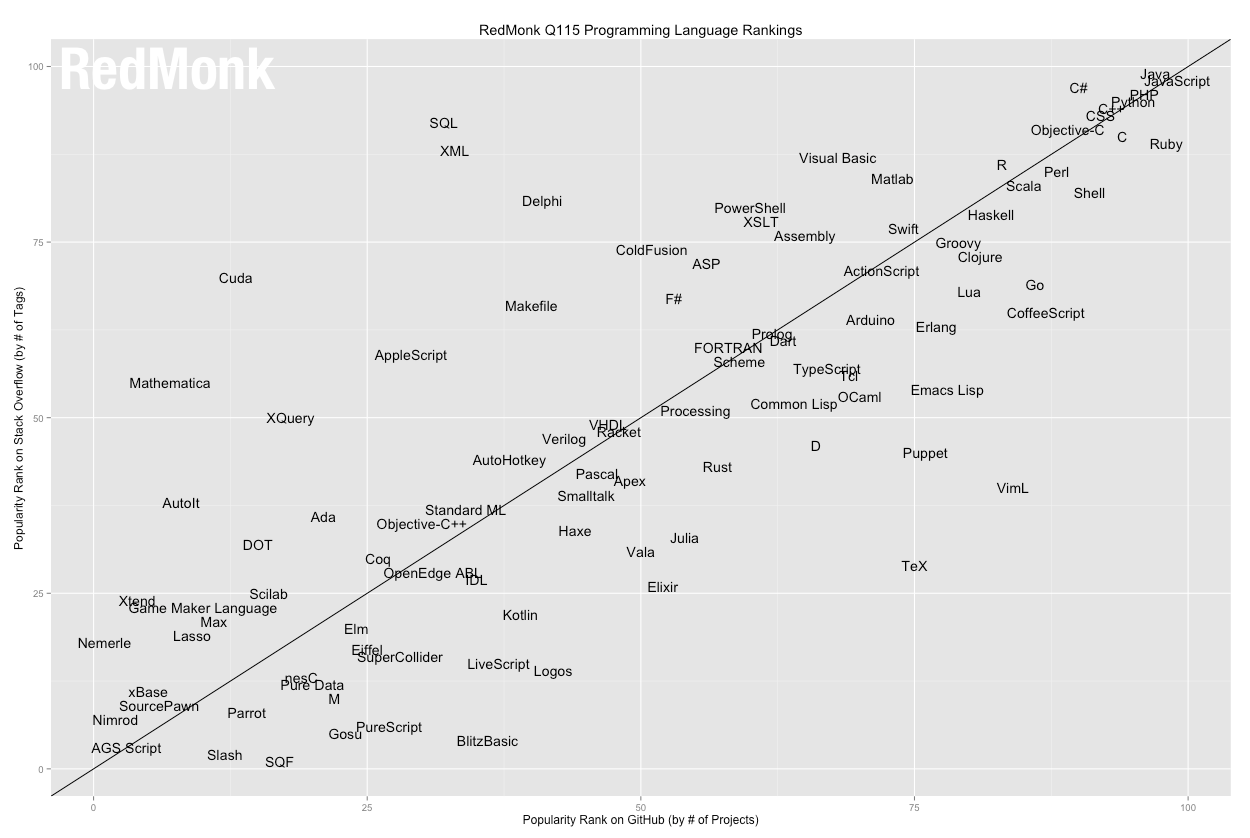
\includegraphics[width=1\textwidth]{img/grafico_redmonk}
	\caption{Ranking das liguagens de programação no Stack Overflow e Github}
\end{figure}


Ainda assim, para compor a interface do dado projeto, também ocorrerá o uso do líder JavaScript de forma intensa, provendo o elo com o as informações gerenciadas pelo PHP.


Entretanto, não seria inteligente desenvolver um sistema completo sem o auxílio de um framework. Dentre os frameworks disponíveis para PHP, hoje o destaque está com o Laravel, que se encontra no topo dentre os mais utilizados no momento. 


A WebHostFace, uma empresa de hospedagem, compilou várias estatísticas para criar um infográfico mostrando os frameworks PHP mais populares de 2015. Utilizando informações sobre os próprios clientes, o Google Trends, estatísticas de repositórios do GitHub e a pesquisa do SitePoint “Best PHP Frameworks 2015”, a WebHostFace elaborou o seguinte infográfico: 

\begin{figure}
	\label{fig:graficoWebhostface}
	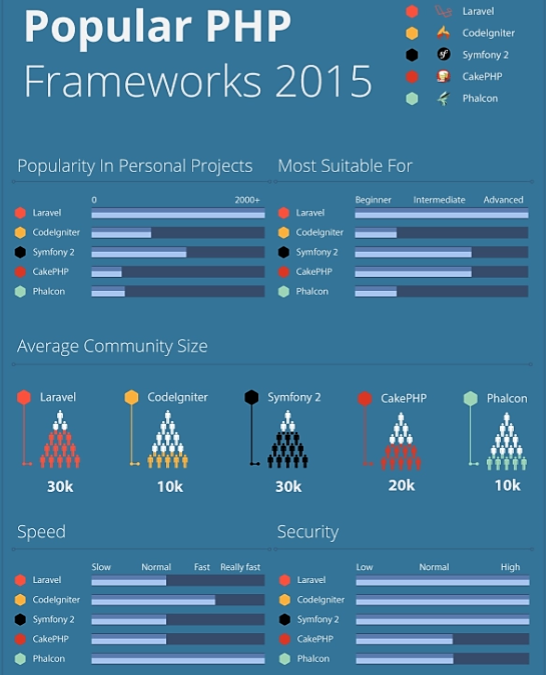
\includegraphics[width=1\textwidth]{img/infografico_webhostface}
	\caption{Infográfico da WebhostFace, exibindo a popularidade dos Frameworks PHP em 2015}
\end{figure}

Assim, tem-se a evidência que o Laravel em 2015 teve a maior popularidade em projetos pessoais e tem a maior comunidade entre os concorrentes, o que o torna uma boa escolha para a escrita de um software que será continuado por terceiros.


Para elaborar os recursos de interface e integrar ao back-end PHP do sistema, será adotado o já conhecido AngularJS, ferramenta sólida e conhecida no aspecto em questão. 


Dados coletados via Google Trends, que propõe comparações entre termos pesquisados, revela a popularidade do AngularJs diante de alguns dos principais concorrentes. O gráfico abaixo evidencia o cenário.


%Como mostra a Figura \ref{fig:graficoGoogleTrendsFerramentasFront}. 
\begin{figure}
	\label{fig:graficoGoogleTrendsFerramentasFront}
	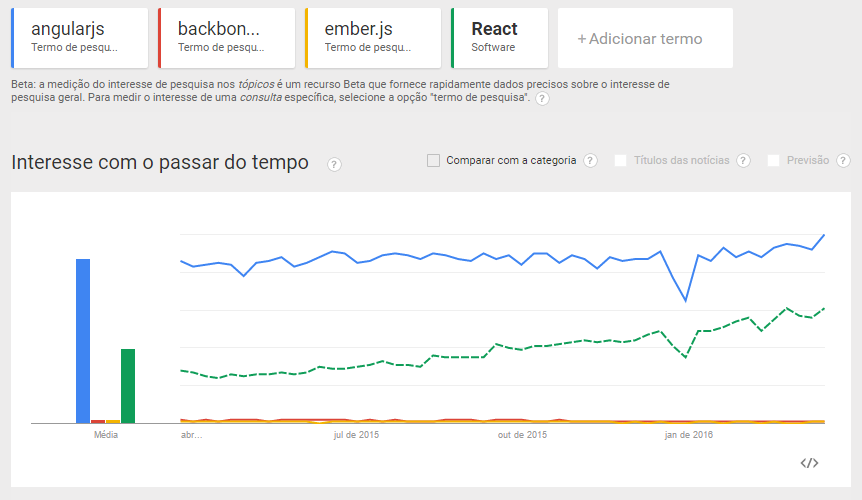
\includegraphics[width=1\textwidth]{img/grafico_ferramentas_front}
	\caption{Gráfico do Google Trends exibindo as pesquisas por ferramentas front-end}
\end{figure}


Junto ao Angular JS, será utilizada a agradável tendência de interface do Material Design da Google, que propõe layouts limpos e otimizados já conhecidos pelos usuários de smartphones Android. 


Para a elaboração da plataforma mobile do projeto, será utilizado o Ionic Framework, muito difundido e bastante pesquisado na área, o que fica evidenciado com o gráfico de pesquisbaixo, coletado via Google Trends buscando por frameworks de desenvolvimento híbrido mobile.


\begin{figure}
	\label{fig:graficoGoogleTrendsFerramentasHibridasMobile}
	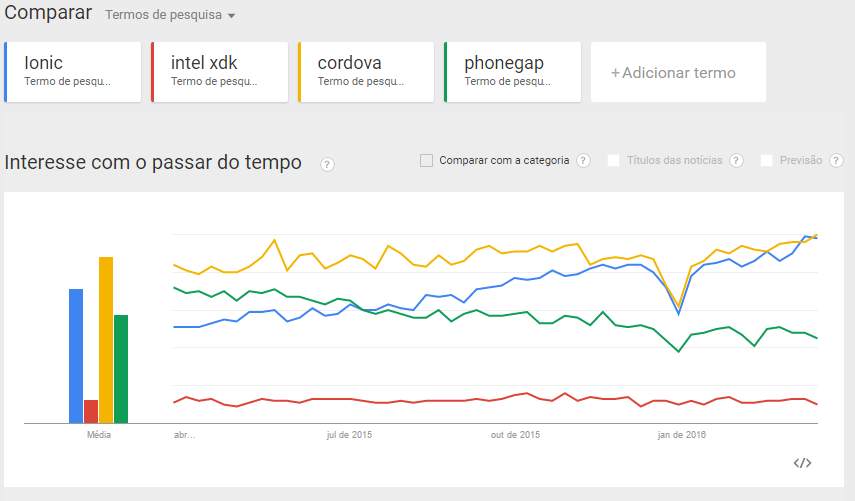
\includegraphics[width=1\textwidth]{img/grafico_ferramentas_hibridas_mobile}
	\caption{Gráfico do Google Trends exibindo as pesquisas por Frameworks híbridos mobile}
\end{figure}	

Para layout da interface mobile, também será aplicado a tendência do Material Design, a fim de propor uma harmonia entre o módulo web e mobile para os usuários


\section{Resultados Esperados}


Como fruto de um sistema para pós-graduação da UFBA, espera-se que os professores tenham mais recursos para integrar as atividades e também prover melhores condições para acompanhamento da vida acadêmica dos alunos em questão. Também, que os novos colaboradores que entrarem no processo tenham facilidade de compreender o fluxo do setor ao navegar pelo sistema proposto.


\section{Fora de Escopo}


Interação com os alunos devido às complicações para realizar a integração com o sistema empregado na UFBA, gerenciado pela XXXXXX, o que causaria uma inviabilidade no projeto devido à necessidade de entrega do produto ser mais forte que o tempo necessário para executar o processo de obtenção de acesso ao sistema legado para realizar a integração.


\section{Estrutura do Trabalho}


<breve resumo sobre os capítulos do TCC>
\chapter{Referencial Teórico}


Projetar o desenvolvimento de um software requer muito planejamento, pois as falhas iniciais podem custar bastante caro ou até mesmo inviabilizar a continuação de um projeto. Assim, a escolha da arquitetura ideal para a aplicabilidade é essencial na concepção de um produto de software. 
De todo o modo, sempre busca-se fazer mais com menos. Diante de tal filosofia, temos nesta seção, uma breve discussão sobre alguns elementos de projeto e arquitetura de software, a fim de contextualizar este trabalho de conclusão de curso.


% Ser direto no começo, focando no que realmente será discutido A seção \ref{sec:apps_mobile} 
 \section{Software como serviço}\label{sec:saas}


A definição de SaaS encontra-se muito bem elaborada em um dos trabalhos listados na literatura. Segundo La e Chun \citep{La2009Systematic}, o princípio da definição de Software como um Serviço (Sofware as a Service - SaaS) é um serviço complementar para aplicações da computação em nuvem (cloud computing). As duas áreas estão interligadas, no entanto, não se confundem, pois o SaaS deve ser entendido como um mecanismo de suporte às soluções existentes na cloud. Os SaaS existem justamente para maximizar o reuso de serviços repetidos e não centrais em uma aplicação remota.


Como propõe vantagens, software como servico é uma tendência forte, isso graças à evolução da web. Diversos fatores podem ser favoráveis para a adoção de um SaaS, como custo e manutenção dentre outros fatores aplicaveis a determinados contextos. Um trabalho recente realizado por Lechessa et al. \cite{LechesaSS11} apresenta uma pesquisa qualitativa sobre os fatores determinantes para adoção ou não de um SaaS voltado para ERP na África do Sul. Esses autores indicam que os principais fatores determinantes para adoção desse mecanismo de software são sua fluidez quanto à rede e a segurança. Esses fatores estão presentes na aplicação desenvolvida neste trabalho de conclusão de curso.
 

Devido ao fato de ter um serviço constantemente na nuvem, fica o questionamento sobre a segurança da informação manipulada. Sabe-se que a vulnerabilidade na web não é restrita ao SaaS, atingindo diversos âmbitos. O artigo de Rai et al. \cite{journals/corr/RaiSM13} orienta como o avanço da computação em nuvem não é um problema apenas para os serviços web do ponto de vista da segurança, pois muitos trabalhos na literatura mostram a área como mais um ponto de vulnerabilidade para diversos setores, a exemplo de infraestrutura. No mesmo artigo mencionado de Rai et al. \cite{journals/corr/RaiSM13}, também realizaram-se estudos exploratórios junto a empresas usuárias de serviços em computação em nuvem e consideram que a perspectiva de SaaS também pode fortalecer a segurança nas aplicações de cloud computing, pois o software de autenticação compartilhado por várias aplicações em nuvem, oferece uma melhor padronização e consequente facilidade de prevenção a erros de vulnerabilidade específicas de cada módulo da pesquisa. Esse ponto de vista é muito importante para qualquer trabalho de ponta na área de SaaS.


A arquitetura de armazenamento de dados de um Saas pode variar de acordo com a necessidade do contexto. O artigo recente de Huixin \cite{7586486}, exemplifica possíveis modelagens para utilizar. Tal abordagem pode ser com um banco de dados único, fazendo com que diferentes clientes compartilhem o mesmo banco, diferindo os dados através de controle de usuário, ou isolando os diferentes clientes através de bancos de dados exclusivos para cada um. Tal fator também pode ser combinado com a arquitetura da aplicação, caso ofereça aplicação única para todos os clientes ou aplicação compartilhada. Diante das possíveis abprdagens, a modelagem de dados do software pode ser decidida pela regra de negócio. Este trabalho optou por aplicação única e banco de dados compartilhado.


Devido ao diferente conceito de obtenção de software, tanto pela visão do cliente como pela visão do vendedor, é necessário tomar conhecimento dos diversos fatores que podem ser relevantes ao orçar um Saas. O recente trabalho de T. Kaur et al. \citep{6949281} orienta um modelo para compor o custo de um Saas. O custo total seria composto pelos fatores que dão suporte ao funcionamento do software. Tais fatores incluem infra-estrutura, configurabilidade, customização, parâmetros de QoS(Quality of service) como escalabilidade, disponibilidade, usabilidade, pontualidade e desempenho da resposta, portabilidade, custo total de propriedade e retorno do investimento. Esses fatores caracterizam o custo de forma eficaz, possibilitando ao fornecedor, prover um Serviço de acordo com a exigência do consumidor em vários pacotes de serviços.


\section{Reuso de software}\label{sec:reuso} %CRUISE BOOK CAPITULO 2


Para Peter Freeman, o reuso é a utilização de qualquer informação que um desenvolvedor pode necessitar no processo de criação de software (Ezran et al., 2002). Basili e Rombach definem reutilização de software como o uso de tudo o que está associado a um projeto de conhecimento (Basili e Rombach, 1991).
Assim, o objetivo da reutilização de software é reciclar o design, código e outros componentes de um produto de software e assim reduzir o custo, o tempo e melhorar a qualidade do produto.
Segundo Keswani et al. \cite{6783445}, o componente reutilizável de software pode ser qualquer parte de seu desenvolvimento, como um fragmento de código, design, casos de teste, ou até mesmo a especificação de requisitos de uma funcionalidade do software. 

O reuso de software pode ter impacto positivo em diversos aspectos do software, vejamos alguns, conforme apresentados no C.R.U.I.S.E Book:

\begin{itemize}

\item Qualidade: As correções de erro tornam-se úteis em todos os locais em que ocorreu, padronizando e facilitando a manutenção.

\item Produtividade: O ganho de produtividade é alcançado devido ao menor número de artefatos desenvolvido. Isso resulta em menos esforços de teste e também economiza análise e design, gerando economia em diversos escopos do projeto.

\item Confiabilidade: A utilização de componentes bem testados aumenta a
confiança no software. Além disso, a utilização de um mesmo componente em vários sistemas, aumenta a possibilidade de detecção de erros e reforça a confiança no componente.

\item Redução do Esforço: A reutilização de software proporciona uma redução do tempo de desenvolvimento, o que reduz o tempo necessário para o produto ser disponibilizado no mercado para trazer rentabilidade.

\item Trabalho redundante e tempo de desenvolvimento: Desenvolver um sistema do
zero significa desenvolvimento redundante de muitos componentes, como requisito
especificações, casos de uso, arquitetura, etc. Isso pode ser evitado quando estes estão disponíveis como componentes reutilizáveis e podem ser compartilhados, resultando em menos desenvolvimento, tempo e custo associado.

\item Documentação: Embora a documentação seja muito importante para a
manutenção de um sistema, muitas vezes é negligenciada. A reutilização de componentes software reduz a quantidade de documentação a ser escrita, entretanto depende da qualidade do que está escrito. Assim, apenas a estrutura do sistema e os novos artefatos desenvolvidos necessitam ser documentados.

\item Custo de manutenção: Menos defeitos e manutenções são esperados quando tem-se comprovada a qualidade dos componentes utilizados.

\item Tamanho da equipe: É comum entrar casos em que a equipe de desenvolvimento sofre sobrecarga. Entretanto, dobrar o tamanho da equipe de desenvolvimento não necessariamente duplica produtividade. Se muitos componentes podem ser reutilizados, é possível desenvolver com equipes menores, levando a melhores comunicações e aumento da produtividade.

\end{itemize}

Apesar dos benefícios da reutilização de software, a mesma não é amplamente praticado como imagina-se. Existem fatores que influenciam direta ou indiretamente na sua adoção. Esses fatores podem ser de aspecto gerencial, organizacional, econômico, conceitual ou técnico. Veremos a seguir alguns aspectos que podem gerar conflito com a cultura de reuso de software, segundo o C.R.U.I.S.E Book:
%(Sametinger, 1997). REVER

\begin{itemize}
	
\item Falta de apoio da gestão: Como a reutilização de software gera custos iniciais,
a medida pode não ser amplamente alcançada em uma organização sem o apoio de alto nível gestão. Os gestores têm de ser informados sobre os custos iniciais e serem convencidos sobre economias futuras.

\item Gerenciamento do Projeto: Gerenciar projetos tradicionais é uma tarefa árdua, principalmente, os que praticam a reutilização de software. Utilizando a técnica em larga escala, tem-se impacto sobre todo o ciclo de vida do software.

\item Estruturas organizacionais inadequadas: As estruturas organizacionais devem
considerar diferentes necessidades que surgem quando a reutilização em larga escala está sendo adotada. Por exemplo, uma equipe particionada pode ser alocada somente para desenvolver, manter e certificar componentes reutilizáveis de software.

\item Incentivos de gestão: É comum a falta de incentivo para deixar os desenvolvedores gastarem tempo elaborando reutilizáveis componentes do sistema. A produtividade é muitas vezes medida apenas no tempo necessário para concluir um projeto. Assim, fazer qualquer trabalho além disso, embora benéfico para a empresa como um todo, diminui o seu sucesso. Mesmo quando os componentes reutilizáveis são utilizados, os benefícios obtidos são uma pequena fração do que poderia ser alcançado caso houvesse reutilização explícita, planejada e organizada.

\item Dificuldade de encontrar software reutilizável: Para reutilizar os componentes, devem existir formas eficientes de busca. Além disso, é importante ter um repositório bem organizado contendo componentes com um eficiente meio de acesso.

\item Não reutilização do software encontrado. O acesso fácil ao software existente
não necessariamente aumentar a reutilização. Os componentes reutilizáveis devem ser cuidadosamente especificados, projetados, implementados e documentados, pois em alguns casos, modificar e adaptar o código  pode ser mais custoso que a programação da funcionalidade necessária a partir do zero.

\item Modificação: É muito difícil encontrar um componente que funcione
exatamente da mesma maneira que queremos. Desta forma, são necessárias modificações e devem existir formas de determinar os seus efeitos sobre o componente.


\end{itemize}


%Outra diretriz importante para a reutilização de software é reduzir o risco na criação de novos softwares. O risco tende a ser bastante reduzido se os componentes que estão sendo reutilizados têm as documentação, interfaces necessárias e devidamente testadas, fatores que contibruem para uma fácil integração.
%De acordo com Keswani et al. \citep{6783445}, para o reuso de software dar retornos apropriados, o processo deve ser sistemático e planejado. Qualquer organização que implemente a reutilização de software deve identificar os melhores métodos e estratégias de reutilização para obter a máxima produtividade. A reutilização de software ajuda a evitar software de engenharia a partir do zero, pois usa módulos de software existentes. A reutilização de software, embora seja uma tarefa difícil, especialmente para softwares antigos sem padrões de projeto, pode melhorar significativamente a produtividade e a qualidade de um produto de software. Embora a reutilização de software não seja um novo campo, ela pode dar grandes retornos em curto período de tempo.


\section{Modularização}\label{sec:modularizacao} %artigo de claudio pagina 222 introdução


%A modularidade vem desempenhando um papel predominante estágios emergentes das disciplinas de arquitetura de software [13]. Engenheiros de software consideram modularidade como princípio base na comparação entre arquiteturas alternativas  e arquitetura degeneração [9]. De fato, os engenheiros de software são incentivados a arquitecturas, baseando-se numa multiplicidade de mecanismos de modularidade disponíveis em: 
%(i) Linguagens de descrição de arquitetura (ADLs), como ACME [8], 
%(ii) catálogos de arquitetônicos [2, 13], e 
%(iii) conhecem bem princípios de alto nível, como interfaces de componentes estreitos, acoplamento arquitectónico reduzido e semelhantes.


Conforme é frisado no trabalho de Wickramaarachchi e Lai \citep{7062705}, o conceito de modularização na indústria de software tem uma longa história e tem sido utilizado para melhorar o processo de desenvolvimento de software em diferentes estágios. Os principais conceitos por trás da modularização do software foram introduzidos por pesquisadores pioneiros há quarenta anos, com uma notável contribuição feita por Melvin Conway e David Parnas, que tem representação notável na engenharia de software.


Modularizar um software é um bom padrão a ser adotado. Segundo Wickramaarachchi e Lai \citep{7062705}, a modularização é importante na identificação de dependências e reduz as dificuldades diante de uma possível necessidade de grandes alterações. De uma perspectiva da engenharia de software, uma modularização geralmente tem várias vantagens, tais como: tornar a complexidade do software mais gerenciável, facilitar o trabalho paralelo e tornar o software mais maleável para acomodar o futuro incerto que um software pode ter. O objetivo final da modularização do software é aumentar a produtividade ea qualidade do software. Tal conceito encontra-se bastante difundido e estái incorporado em linguagens de programação e ferramentas de software. O trabalho proposto favorece ao uso da modularização de um software e até mesmo pode ser considerado um módulo a ser acoplado a qualquer software, mediante a compatibilidade.


\section{Aplicações web}\label{sec:apps_web}


A popularidade da aplicação web aumentou exponencialmente na última década e todos os dias cresce o número de pessoas usuárias de aplicações web. E seguindo o padrão de desenvolvimento de software, Kumar et al. \citep{7813710} sugerem que para o desenvolvimento web, deve-se manter a prática efiacaz de produzir diagramas UML. A abordagem baseada na web oferece uma maneira fácil e eficaz para gerenciar e controlar o processo de desenvolvimento por meio de diagramas UML. Tal abordagem pode ser usada quando há uma exigência de lidar com mudanças muito rápidas e grandes em requisitos de forma muito eficaz em muito menos tempo, gerando assim um menor impacto. 


Para atender à fomentada demanda de aplicativos web, é necessário adotar métodos de desenvolvimentos que sejam ágeis, eficientes e de fácil manutenção. Yu Ping et al. \cite{1372143} propõem o uso do modelo MVC (Model, View e Controller) no atual desenvolvimento para softwares web. O modelo apresentado tornou-se um padrão popular e divide o software em camadas com propósito definido, tornando-o de mais fácil manutenção.


O Ajax (Asynchronous Javascript and XML) revolucionou a web. Conforme demonstrado no artigo de Yuping \citep{6845605}, ao usar a tecnologia Ajax, podemos enriquecer a experiência do usuário em aplicações baseadas em navegador de internet, e fornecer uma variedade de aplicações interativas para atender às necessidade de humanização das aplicações.
Os aplicativos Ajax em execução no navegador se comunicam com um servidor Web de forma assíncrona e atualizam apenas uma parte da página.


\chapter{Proposta}


A adoção de padrões é uma premissa básica para o desenvolvimento de software, pois ao trabalhar com variações dentro de uma organização, a tendência é gerar confusão. Assim, o objetivo deste trabalho é projetar e implementar um módulo padrão de permissões de acesso, de modo que o mesmo possa ser utilizado por diferentes plataformas, como desktop, Web e mobile, eliminando assim este módulo do desenvolvimento de um software e utilizando o trabalho proposto como um SaaS provedor das permissões do software cliente a ser desenvolvido.


É comum encontrar frameworks de desenvolvimento de software que automatizam a geração de esquemas de configuração de módulos com perfis de acesso. Entretanto, apesar de ser um facilitador, tal política pode se tornar confusa em algus cenários, a exemplo de uma empresa que trabalha com sistemas sob encomenda, onde o cliente pode até mesmo determinar a linguagem ou framework de desenvolvimento. Nesse caso, a empresa teria que treinar os seus colaboradores a configurar os softwares para cada uma das ferramentas utilizadas, o que potencialmente ocasionaria dificuldades de entendimento comum.


Diante da possibilidade de manter a configuração dos sistemas de uma mesma instituição com diferentes módulos de permissão, seria ideal que todos os sistemas de software por ela desenvolvidos utilizassem um mesmo módulo de configuração de persmissão de acesso, para que esta parte comum, presente na maioria dos softwares, fosse padronizada.


O capítulo corrente é composto por três seções. A seção \ref{sec:arquitetura} trata da arquitetura do software proposto, contendo informações sobre as tecnologias utilizadas, diagramas UML e os requisitos do sistema. A seção \ref{sec:processo} demonstra o fluxo do processo empregado na aplicação desenvolvida e por fim, a seção \ref{sec:novidades} trada do que há de novo sob o ponto de vista tecnológico.

\section{Arquitetura da aplicação}\label{sec:arquitetura}


A aplicação desenvolvida neste trabalho foi arquitetada com o modelo SPA(Single page application) utilizando o AngularJs. Tal arquitetura se tornou tão popular quanto o famoso MVC (Model-View-Controller), e é bastante utilizada no desenvolvimento de aplicações web e mobile. Em linhas gerais, o conceito SPA tende a reduzir a necessidade de se implementar código server-side, e sim potencializar as ações em client-side. Assim, boa parte da aplicação passa a ser processada no cliente (dentro do navegador Web).


%\begin{figure}
%	\label{fig:spa}
%	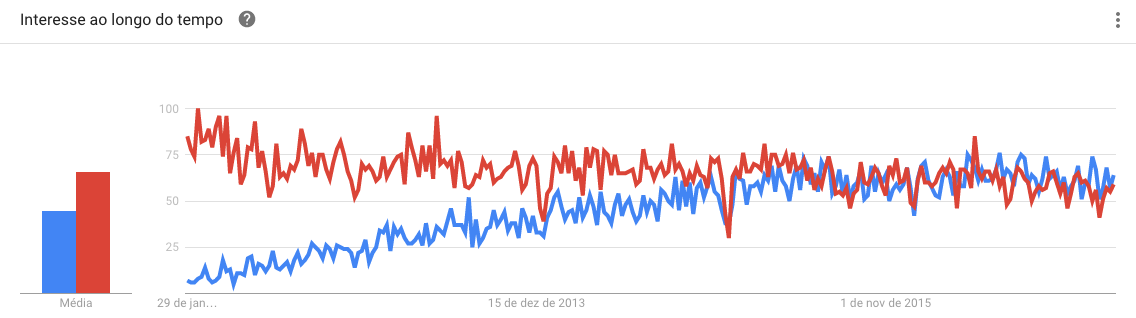
\includegraphics[width=1\textwidth]{img/spa-mvc}
%	\caption{Gráfico do Google Trends exibindo comparação entre as pesquisas por SPA e MVC}
%\end{figure}
não faça simplesmente copiar de um blog. tente ir além, e prover fundamentação contida em livros-texto da área.
um sugestão: capture as ideias do autor do blog, porém complemente-as com outras fontes, assegurando-se de que o que o autor do blog descreve de fato faz sentido na prática

Algumas vantagens da SPA:
\begin{itemize}

\item Partilha de processamento do software, visto que a aplicação consome uma API REST(back-end) e deve tratar os dados para a exibição no front-end.
\item Com da partilha do processamento, tem-se uma menor codificação no servidor. Tal aspecto vem acompanhado com a distinção das responsabilidades, pois apenas o código do front-end trata de interface.
\item Diante das características de uma SPA, a "página única" tende a ser de fácil entendimento aos usuários, simplificando a navegação.
\item Como os acessos via dispositivos móveis é bastante significativo, há uma relevância no consumo de dados do software. Nesse quesito, uma SPA se comporta bem, devido à forma como consome os dados, com requisições AJAX que retornam JSON(Javascript object notation), que na realidade se resume apenas a dados estruturados.

\end{itemize}
O grande ator de app SPA é o código Javascript executado no cliente. Toda a aplicação pode ser construída simplesmente manipulando-se o DOM (Document Object Model) de forma nativa, ou com o uso de bibliotecas e frameworks Javascript que auxiliam na construção da aplicação. Estas bibliotecas e frameworks fornecem recursos para manipulação dinâmica do DOM, definição de templates de tela, chamadas assíncronas ao servidor, organização do código Javascript, etc. Dentres as diversas bibliotecas Javascript disponíveis, tem-se entre as mais difundidas: AngularJs\footnote{https://angularjs.org/}
, VueJs\footnote{https://vuejs.org/}, Backbone\footnote{http://backbonejs.org/}, ReactJs\footnote{https://facebook.github.io/react/}, Ember\footnote{http://emberjs.com/} e outras.


Do lado servidor, tem-se a execução das linguagens de programação tradicionais como PHP, ASP.NET, JSP e etc. Assim, de acordo com a necessidade, as mesmas provêem host de arquivos, acesso a banco de dados e tratam regras de negócios que não podem estar no código JavaScript do Front-end por questões de segurança. E é do lado servidor que a arquitetura REST (Representational State Transfer) pode ser utilizada, com o intuito de fornecer serviços do servidor à aplicação SPA proposta neste trabalho. É comum encontrar aplicação SPA utilizando serviços RESTFul. Uma aplicação no servidor que utiliza a arquitetura REST para prover serviços, então é chamada de RESTFul. Neste trabalho, foi desenvolvida uma aplicação RESTFul com o Framework PHP Laravel.


Ao construir uma aplicação utilizando a arquitetura REST, o protocolo HTTP é usado em sua essência, utilizando os métodos de requisição ao servidor: GET, POST, PUT e DELETE (os mais comuns), e cada um deles indica uma determinada ação a ser executada em um recurso específico do servidor.


A seguir, a subseção \ref{tecnologias} trata das tecnologias utilizadas no trabalho proposto, a \ref{diagramas} apresenta os diagramas UML do projeto e \ref{funcionalidades} trata das funcionalidades, formalizando os requisitos funcionais e não funcionais.


\subsection{Tecnologias utilizadas}\label{tecnologias}


\subsubsection{Laravel framework}


Laravel \footnote{https://laravel.com/} é um framework PHP livre e open-source para o desenvolvimento de sistemas Web que utilizam o padrão MVC (model, view, controller). O Laravel foi desenvolvido sob o MIT License, com o código-fonte hospedado no GitHub. Em Agosto de 2015, o Laravel já era o principal framework de projetos PHP no GitHub. 


Algumas características proeminentes do Laravel são sua sintaxe simples e concisa, um sistema modular com gerenciador de dependências dedicado, várias formas de acesso a banco de dados relacionais e vários utilitários indispensáveis no auxílio ao desenvolvimento e manutenção de sistemas. Diante da popularidade do framework, tem-se uma grande comunidade, o que facilita a aprendizgem pois facilmente encontra-se tutoriais. Inclusive além da documentação, o próprio Laravel disponibiliza o Laracasts \footnote{https://laracasts.com/}, que traz aos desenvolvedores uma série de vídeos ensinando as mais diversas funcionalidades encontradas no Laravel.


\subsubsection{AngularJs}


AngularJS é um framework JavaScript open-source, mantido por Google, que auxilia na execução de SPA. O framework lê o HTML que contém tags especiais do framework e então executa a diretiva na qual esta tag pertence, e faz a ligação entre a apresentação e seu modelo, representado por variáveis JavaScript comuns. O framework adapta e estende o HTML tradicional para uma melhor experiência com conteúdo dinâmico, com a ligação direta e associação bidirecional dos dados (two-way data-binding) que permite sincronização automática de models e views. Como resultado, AngularJS abstrai a manipulação do DOM e melhora os testes.


\subsubsection{Bootstrap}


Bootstrap é um popular framework front-end que facilita a criação de sites com tecnologia responsiva.
O Bootstrap possui diversos componentes (plugins) em JavaScript (jQuery) que auxiliam o desenvolvedor a implementar, menu-dropdown, modal, carousel, slideshow, entre outros com facilidade, apenas acrescentando algumas configurações no código.


\subsection{Diagramas}\label{diagramas}


Nesta seção, temos a apresentação de alguns diagramas UML (Unified Modeling Language) com a finalidade de embasar o trabalho proposto, permitindo representar o sistema de forma padronizada.


A imagem \ref{fig:Diagrama de caso de uso} traz o diagrama de casos de caso, com o objetivo de os usuários obterem melhor entendimento das principais funcionalidades de  sistema.


\begin{figure}
	\label{fig:Diagrama de caso de uso}
	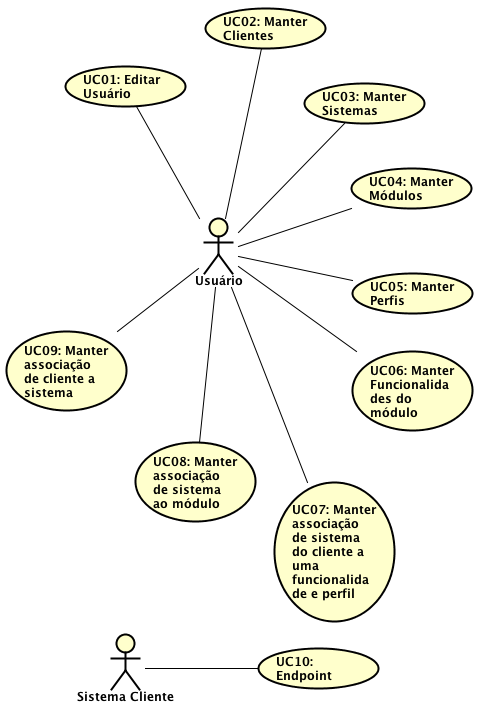
\includegraphics[width=1\textwidth]{img/Diagrama_de_caso_de_uso}
	\caption{Diagrama de caso de uso}
\end{figure}


Com a imagem \ref{fig:Diagrama de classe}, é possível compreender com mais clareza o funcionamento do back-end do software, visualizando as classes utilizadas para manipular os dados.

\begin{figure}
	\label{fig:Diagrama de classe}
	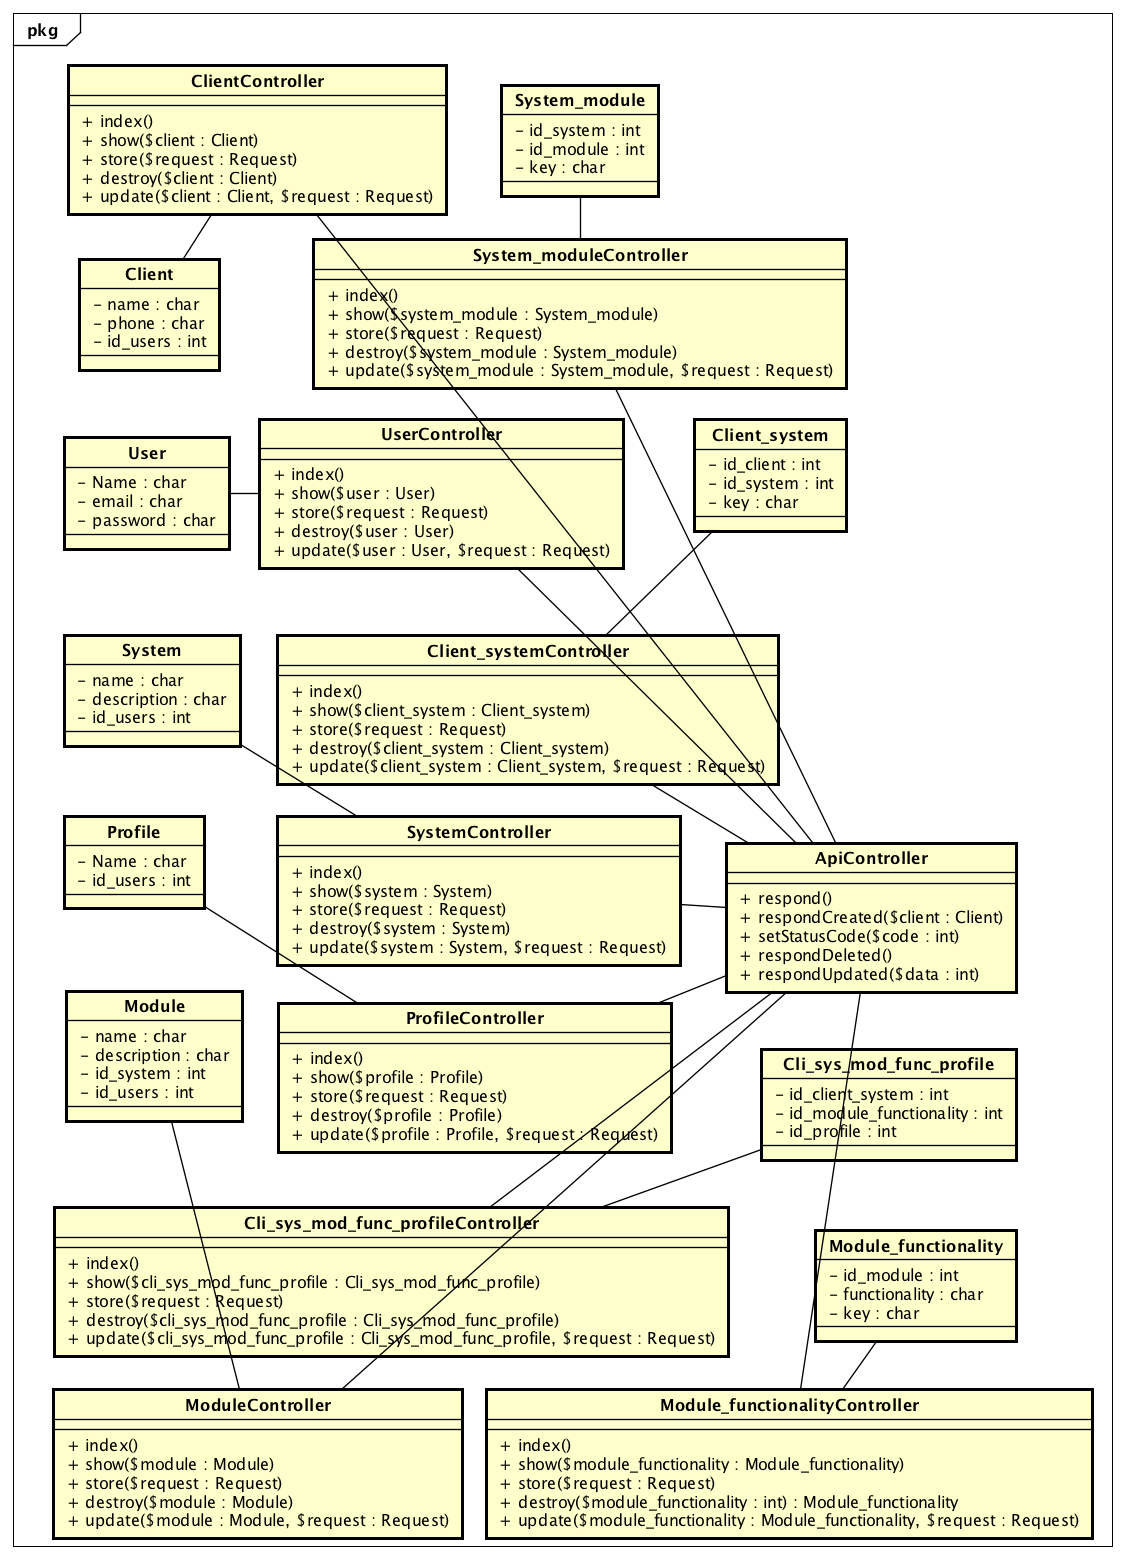
\includegraphics[width=1\textwidth]{img/Diagrama_de_classe}
	\caption{Diagrama de classe}
\end{figure}


Por fim, para prover um entendimento de funcionamento interno do software, a imagem \ref{fig:DER} traz o diagrama de entidade relacionamento, fornecendo uma ilustração da organização do banco de dados utilizado.


\begin{figure}
	\label{fig:DER}
	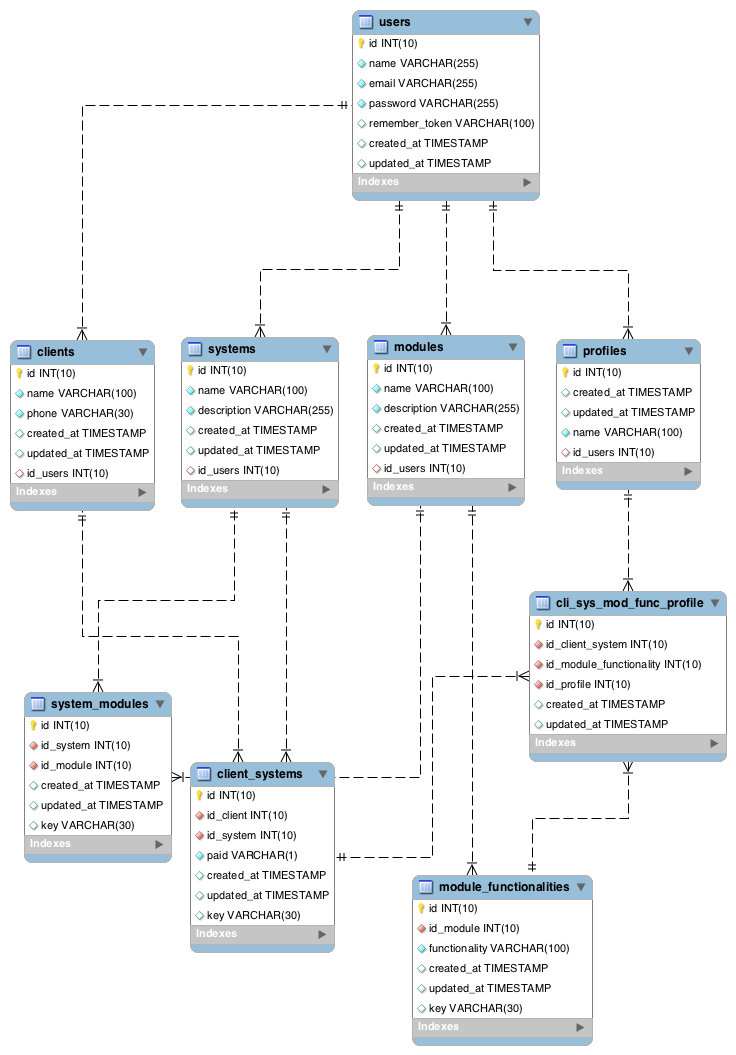
\includegraphics[width=1\textwidth]{img/DER}
	\caption{Diagrama entidade relacionamento}
\end{figure}


\subsection{Funcionalidades}\label{funcionalidades}

Esta seção apresenta os requisitos funcionais e não-funcionais implementados na aplicação proposta neste trabalho.


\subsubsection{Requisitos não funcionais}



\begin{itemize}
	
	
\item RN01: Usuários Simultâneos


Descrição: O sistema deverá suportar processamento multiusuário, ou seja, vários usuários poderão utilizar o sistema simultaneamente. 


\item RN02: Segurança 


Descrição: O sistema só permitirá acesso aos dados com autorização. Os usuários deverão se identificar usando um login e uma senha, e a referida senha será criptografada com a metodologia Bcrypt no banco de dados.


\item RN03: Alta disponibilidade 


Descrição: O sistema deverá ter disponibilidade de aproximadamente 99 porcento do tempo, a ser verificado com os logs do servidor.


\item RN04: Desempenho


Descrição: O tempo de resposta das consultas não deve ultrapassar 3 segundos, a ser validado com teste ao em produção.


\end{itemize}
	

\subsubsection{Requisitos funcionais}


\begin{itemize}
	
	
\item RF 01: Login


Descrição: O sistema deve conter tela de login com os campos email e senha. Após inserção dos dados, o sistema deve validar os dados e caso positivo, encaminhar o usuário ao sistema. Caso os dados sejam inválidos, exibir mensagem de erro para o usuário.


\item RF 02: Edição de usuário


Descrição: O sistema deve conter um formulário que seja carregado com os dados do usuário da sessão e permitir a atualização dos dados. Este requisito está relacionado ao UC01 da imagem \ref{fig:Diagrama de caso de uso}.


\item RF 03: Cadastro de cliente


Descrição: O sistema deve conter um formulário para cadastro de clientes. Após a inserção de um registro, o sistema deve automaticamente exibir o registro em formato de edição e conter botão para ir a uma consulta que liste os clientes cadastrados para o usuário da sessão. Este requisito está relacionado ao UC02 da imagem \ref{fig:Diagrama de caso de uso}.


\item RF 04: Cadastro de sistema


Descrição: O sistema deve conter um formulário para cadastro de sistemas. Após a inserção de um registro, o sistema deve automaticamente exibir o registro em formato de edição e conter botão para ir a uma consulta que liste os sistemas cadastrados para o usuário da sessão. Este requisito está relacionado ao UC03 da imagem \ref{fig:Diagrama de caso de uso}.


\item RF 05: Cadastro de módulo


Descrição: O sistema deve conter um formulário para cadastro de módulos. Após a inserção de um registro, o sistema deve automaticamente exibir o registro em formato de edição e conter botão para ir a uma consulta que liste os módulos cadastrados para o usuário da sessão. Este requisito está relacionado ao UC04 da imagem \ref{fig:Diagrama de caso de uso}.


\item RF 06: Cadastro de perfil


Descrição: O sistema deve conter um formulário para cadastro de perfil. Após a inserção de um registro, o sistema deve automaticamente exibir o registro em formato de edição e conter botão para ir a uma consulta que liste os perfils cadastrados para o usuário da sessão. Este requisito está relacionado ao UC05 da imagem \ref{fig:Diagrama de caso de uso}.


\item RF 07: Cadastro associativo de cliente aos sistemas


Descrição: O sistema deve conter um formulário para cadastro associativo de clientes a sistemas. Após a inserção de um registro, o sistema deve automaticamente gerar uma chave de acesso do dado registro para o usuário consultar permissões e exibir o registro em formato de edição e conter botão para ir a uma consulta que liste os registros associativos de clientes aos sistemas cadastrados para o usuário da sessão. Este requisito está relacionado ao UC09 da imagem \ref{fig:Diagrama de caso de uso}.


\item RF 08: Cadastro associativo de  sistemas aos módulos


Descrição: O sistema deve conter um formulário para cadastro associativo de sistemas a módulos. Após a inserção de um registro, o sistema deve automaticamente gerar uma chave de acesso do dado registro para o usuário consultar permissões e exibir o registro em formato de edição e conter botão para ir a uma consulta que liste os registros associativos de  sistemas aos módulos cadastrados para o usuário da sessão. Este requisito está relacionado ao UC08 da imagem \ref{fig:Diagrama de caso de uso}.


\item RF 09: Cadastro de funcionalidade dos módulos


Descrição: O sistema deve conter um formulário para cadastro de funcionalidade dos módulos já cadastrados. Após a inserção de um registro, o sistema deve automaticamente gerar uma chave de acesso do dado registro para o usuário consultar permissões e exibir o registro em formato de edição e conter botão para ir a uma consulta que liste os registros de funcionalidades cadastradas para o usuário da sessão. Este requisito está relacionado ao UC06 da imagem \ref{fig:Diagrama de caso de uso}.


\item RF 10: Composição de permissão para os módulos dos clientes


Descrição: O sistema deve conter um formulário para cadastro associativo de permissão para os módulos dos clientes. Após a inserção de um registro, o sistema deve automaticamente exibir o registro em formato de edição e conter botão para ir a uma consulta que liste os registros associativos de permissão cadastrados para o usuário da sessão. Este requisito está relacionado ao UC07 da imagem \ref{fig:Diagrama de caso de uso}.


\item RF 11: Endpoint


Descrição: O sistema deve disponibilizar uma URL para receber uma requisição via post, onde o deve receber um parâmetro "key", contendo a chave de acesso desejada para consultar as permissões cadastradas. Ao realizar a requisiçao enviando a "key", o sistema deve retornar um texto no formato Json, contendo os dados das permissões que foram compostas no sistema pelo usuário. A chave enviada pelo usuário pode ser de qualquer um dos níveis de configuração realizado no sistema e o o endpoint deve retornar a resposta sempre num mesmo formato, viabilizando um tratamento único da resposta pelo cliente. Este requisito está relacionado ao UC10 da imagem \ref{fig:Diagrama de caso de uso}.


\end{itemize}

\section{Processo}\label{sec:processo}


Para melhor compreensão do sistema proposto, a figura \ref{fig:diagramaBpmn} apresenta uma visão geral do processo implementado na ferramenta, utilizando, para tal, a notação BPMN.


\begin{figure} %\landscape 
	\vspace*{-2cm}
	\makebox[\linewidth]{
		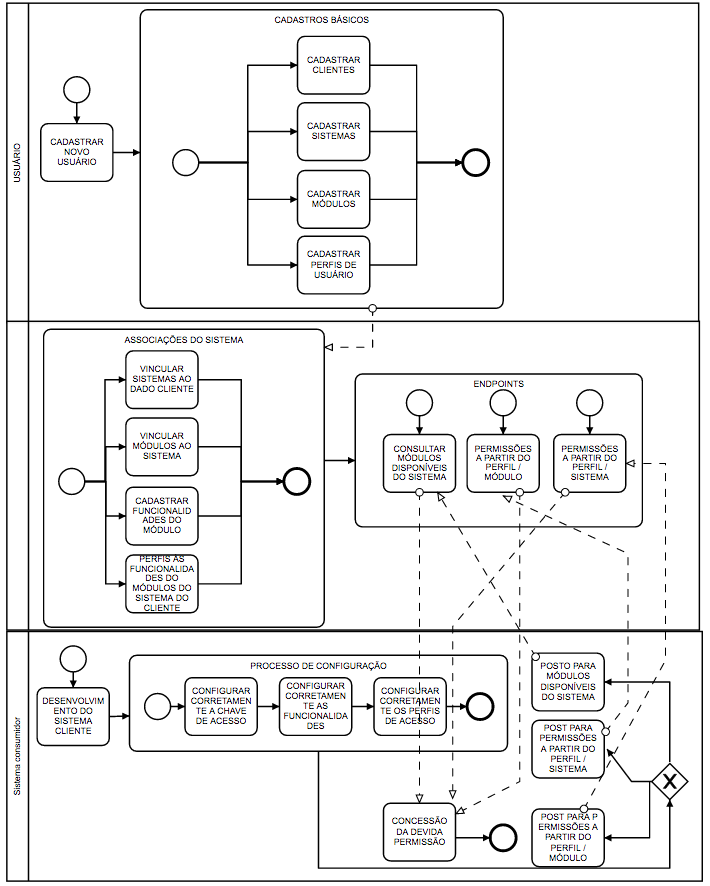
\includegraphics[width=1.3\linewidth]{img/diagrama_bpmn}
	}
	\label{fig:diagramaBpmn}
	\caption{Diagrama do processo(BPMN) do software em questão}
\end{figure}


\section{O que há de novo ?}\label{sec:novidades} %Sob o ponto de vista tecnológico


Seguindo a norma de padranização de código, com o software proposto é possível unificar o módulo de permissões de acesso e tratá-lo como um serviço, tornando possível eliminá-lo de qualquer software que faça uso do mesmo. A bordagem proposta neste trabalho de conclusão não é trivial, trata-se de uma aplicabilidade diferente do controle de permissão dos perfis, que não foi adotado por nenhum sistema disponível no estado da prática.

% %% RiSE Latex Template - version 0.5
%%
%% RiSE's latex template for thesis and dissertations
%% http://risetemplate.sourceforge.net
%%
%% (c) 2012 Yguaratã Cerqueira Cavalcanti (yguarata@gmail.com)
%%          Vinicius Cardoso Garcia (vinicius.garcia@gmail.com)
%%
%% This document was initially based on UFPEThesis template, from Paulo Gustavo
%% S. Fonseca.
%%
%% ACKNOWLEDGEMENTS
%%
%% We would like to thanks the RiSE's researchers community, the 
%% students from Federal University of Pernambuco, and other users that have
%% been contributing to this projects with comments and patches.
%%
%% GENERAL INSTRUCTIONS
%%
%% We strongly recommend you to compile your documents using pdflatex command.
%% It is also recommend use the texlipse plugin for Eclipse to edit your documents.
%%
%% Options for \documentclass command:
%%         * Idiom
%%           pt   - Portguese (default)
%%           en   - English
%%
%%         * Text type
%%           bsc  - B.Sc. Thesis
%%           msc  - M.Sc. Thesis (default)
%%           qual - PHD qualification (not tested yet)
%%           prop - PHD proposal (not tested yet)
%%           phd  - PHD thesis
%%
%%         * Media
%%           scr  - to eletronic version (PDF) / see the users guide
%%
%%         * Pagination
%%           oneside - unique face press
%%           twoside - two faces press
%%
%%		   * Line spacing
%%           singlespacing  - the same as using \linespread{1}
%%           onehalfspacing - the same as using \linespread{1.3}
%%           doublespacing  - the same as using \linespread{1.6}
%%
%% Reference commands. Use the following commands to make references in your
%% text:
%%          \figref  -- for Figure reference
%%          \tabref  -- for Table reference
%%          \eqnref  -- for equation reference
%%          \chapref -- for chapter reference
%%          \secref  -- for section reference
%%          \appref  -- for appendix reference
%%          \axiref  -- for axiom reference
%%          \conjref -- for conjecture reference
%%          \defref  -- for definition reference
%%          \lemref  -- for lemma reference
%%          \theoref -- for theorem reference
%%          \corref  -- for corollary reference
%%          \propref -- for proprosition reference
%%          \pgref   -- for page reference
%%
%%          Example: See \chapref{chap:introduction}. It will produce 
%%                   'See Chapter 1', in case of English language.

\documentclass[pt,twoside,onehalfspacing,bsc]{risethesis}

\usepackage[utf8]{inputenc}
\usepackage[brazilian]{babel}
\usepackage[T1]{fontenc}

%% Change the following pdf author attribute name to your name.
\usepackage[linkcolor=blue,citecolor=blue,urlcolor=blue,colorlinks,pdfpagelabels,pdftitle={Bruno Cabral's Bachelor Thesis},pdfauthor={Bruno Cabral}]{hyperref}

\address{SALVADOR}

\universitypt{Universidade Federal da Bahia}
\universityen{Federal University of Bahia}

\departmentpt{Depertamento de Ciência da Computação}
\departmenten{Computer Science Department}

\programpt{Programa Multiinstitucional de Pós-graduação em Ciência da Computação}
\programen{Graduate in Computer Science}

\majorfieldpt{Ciência da Computação}
\majorfielden{Computer Science}

\title{Sistema de apoio à Pós graduação - UFBA}
\date{Outubro/2016}

\author{Victor de Azevedo Nunes}
\adviser{Ivan do Carmo Machado}

\begin{document}

\frontmatter
\frontpage
\presentationpage

\begin{dedicatory}
Eu dedico esta dissertação...
%I dedicate this dissertation to my family, girlfriend, friends and
%professors who gave me all necessary support to get here.
\end{dedicatory}

\acknowledgements
Meus agradecimentos...

\begin{epigraph}[]{Edward V Berard}
Walking on water and developing software from a specification are easy if both are frozen
\end{epigraph}

\resumo
% Escreva seu resumo no arquivo resumo.tex
Meu resumo

\begin{keywords}
palavras chave

\end{keywords}

\abstract
% Write your abstract in a file called abstract.tex
My abstract...

\begin{keywords}
key words...
\end{keywords}

% Summary (tables of contents)
\tableofcontents

% List of figures
\listoffigures

% List of tables
\listoftables

% List of acronyms
% Acronyms manual: http://linorg.usp.br/CTAN/macros/latex/contrib/acronym/acronym.pdf
\listofacronyms
\begin{acronym}[ACRONYM] 
% Change the word ACRONYM above to change the acronym column width.
% The column width is equals to the width of the word that you put.
% Read the manual about acronym package for more examples:
%   http://linorg.usp.br/CTAN/macros/latex/contrib/acronym/acronym.pdf

\acro{SPA}{Single Page Application}
\acro{JSON}{Javascript Object Notation}
\acro{PHP}{PHP: Hypertext Preprocessor}
\acro{SaaS}{Software as a Service}
\acro{ERP}{Enterprise Resource Planning}
\acro{QoS}{Quality of Service}
\acro{UML}{Unified Modeling Language}
\acro{MVC}{Model-View-Controller}
\acro{Ajax}{Asynchronous Javascript and XML}
\acro{HTML}{HyperText Markup Language}
\acro{CSS}{Cascading Style Sheets}
\acro{API}{Application Programming Interface}
\acro{DOM}{Document Object Model}
\acro{BPMN}{Business Process Model and Notation}
\acro{REST}{Representational State Transfer}

\end{acronym}

% List of listings
%\lstlistoflistings

\mainmatter

\chapter{Introdução}

\section{Motivação}

Organizar os procedimentos de um processo sempre nos traz vantagens. Apesar de no processo de implantação de um sistema, o mesmo burocratizar o processo, com o tempo temos o retorno da dedicação para a inserção dos dados. Com um certo volume de dados, é possível estruturar informações que num processo manual são difíceis de serem enxergadas. Assim, é possível depender menos das pessoas que organizam o processo, pois o legado de informações não estará mais somente na mente de alguns, mas sim documentado nos dados do sistema.

Além de colaborar na organização, também haverá uma grande colaboração no tempo gasto na gestão. Lidar com muitos papéis e confiar na mente humana para guardar informações, não é uma alternativa muito segura devido ao fato que as pessoas sempre estão sujeitas a sair do processo e levar contigo a experiência obtida. Experiência essa que faz com que os procedimentos sejam executados de forma mais eficiente. Entretanto, com um sistema inteligente, é possível auxiliar e tornar mais ágil a execução das tarefas.


\section{Problema}


De acordo com funcionários ligados ao o setor de pós graduação da UFBA, entrevistados a fim de um maior entendimento do cenário, apesar das semelhanças estruturais, a pós graduação gerida de forma diferencia da graduação. FULANO afirma que devido ao fato de não ter a mesma visibilidade, não tem acesso aos mesmos recursos de gestão acadêmica da graduação. O professores não executam somente atividades dentro da sala de aula, também tem diversas outras ocupações no setor. E muitos procedimentos realizados extra classe ainda se encontram sendo realizados de forma manual, estando mais vulnerável ao erro ou até mesmo à violação do processo. Também ocorre um grande desperdício de tempo pelos professores e gestores da área, devido ao diversos processos ainda realizados de forma manual, sem a devida documentação. Segundo FULANO, também entrevistado, esse tempo perdido implica numa redução da eficiência na sala de aula, pois o professor acaba por ter menos tempo disponível para o planejamento das atividades, o que gera impactos negativos aos alunos.


\section{Objetivos} %<o que deve ser feito/entregue>


Devido aos muitos processos sendo resolvidos de forma manual, propõe-se com solução um sistema moderno, arquitetado para ter funcionamento na web e com um módulo mobile, a fim de fornecer informações de forma rápida e eficiente para os professores através de notificações, já que o acesso à internet móvel é comum entre os possíveis usuários do sistema em questão.
O principal requisito para o sistema seria dispor recursos para reduzir o tempo desperdiçado pelos professores durante as atividades extra classe.


\section{Metodologia} %<como será feito | como resolver o problema apontado inicialmente>


%<analise de literatura | design | implementação | validação>
Baseando-se nas tecnologias gratuitas em alta no cenário atual do desenvolvimento web, dispomos de algumas opções eficientes para a implementação da solução. Dentre as possibilidades, considerando a facilidade para futura manutenção e continuidade do projeto, tende-se a optar por uma tecnologia popular. Como linguagem de programação, adota-se o PHP. A escolha é fundamentada de acordo com a pesquisa da RedMonk de 2015, que evidencia o uso das linguagens de programação de acordo com as discussões no StackOverflow e repositórios no GitHub. É possível constatar a popularidade do PHP no cenário atual com o gráfico da pesquisa citada, na qual o PHP é apresentado na terceira colocação, apenas atrás do lider JavaScript e do segundo colocado, o Java.

\begin{figure}
	\label{fig:graficoRedmonk}
	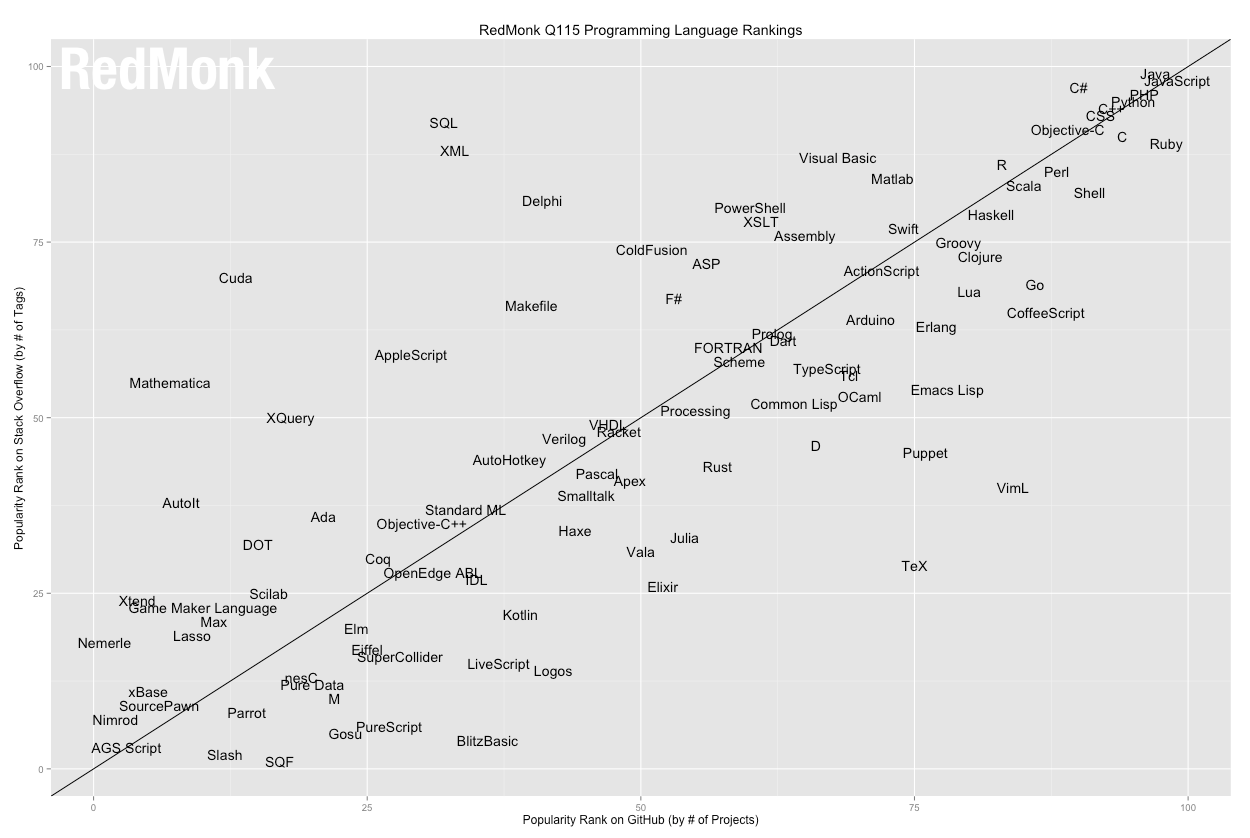
\includegraphics[width=1\textwidth]{img/grafico_redmonk}
	\caption{Ranking das liguagens de programação no Stack Overflow e Github}
\end{figure}


Ainda assim, para compor a interface do dado projeto, também ocorrerá o uso do líder JavaScript de forma intensa, provendo o elo com o as informações gerenciadas pelo PHP.


Entretanto, não seria inteligente desenvolver um sistema completo sem o auxílio de um framework. Dentre os frameworks disponíveis para PHP, hoje o destaque está com o Laravel, que se encontra no topo dentre os mais utilizados no momento. 


A WebHostFace, uma empresa de hospedagem, compilou várias estatísticas para criar um infográfico mostrando os frameworks PHP mais populares de 2015. Utilizando informações sobre os próprios clientes, o Google Trends, estatísticas de repositórios do GitHub e a pesquisa do SitePoint “Best PHP Frameworks 2015”, a WebHostFace elaborou o seguinte infográfico: 

\begin{figure}
	\label{fig:graficoWebhostface}
	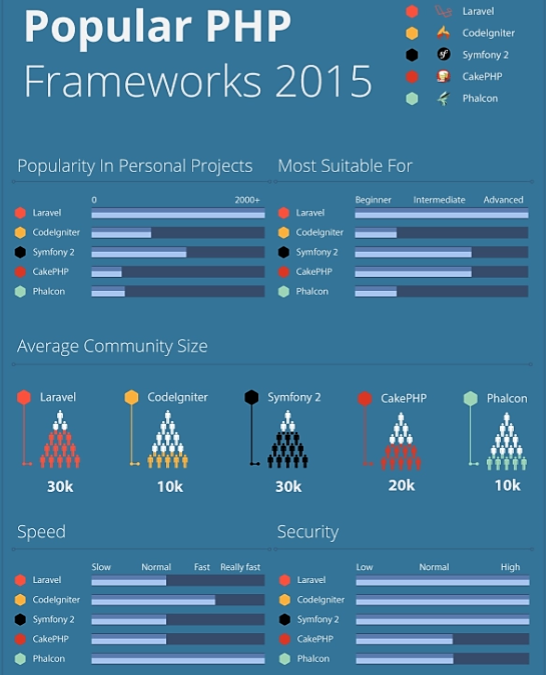
\includegraphics[width=1\textwidth]{img/infografico_webhostface}
	\caption{Infográfico da WebhostFace, exibindo a popularidade dos Frameworks PHP em 2015}
\end{figure}

Assim, tem-se a evidência que o Laravel em 2015 teve a maior popularidade em projetos pessoais e tem a maior comunidade entre os concorrentes, o que o torna uma boa escolha para a escrita de um software que será continuado por terceiros.


Para elaborar os recursos de interface e integrar ao back-end PHP do sistema, será adotado o já conhecido AngularJS, ferramenta sólida e conhecida no aspecto em questão. 


Dados coletados via Google Trends, que propõe comparações entre termos pesquisados, revela a popularidade do AngularJs diante de alguns dos principais concorrentes. O gráfico abaixo evidencia o cenário.


%Como mostra a Figura \ref{fig:graficoGoogleTrendsFerramentasFront}. 
\begin{figure}
	\label{fig:graficoGoogleTrendsFerramentasFront}
	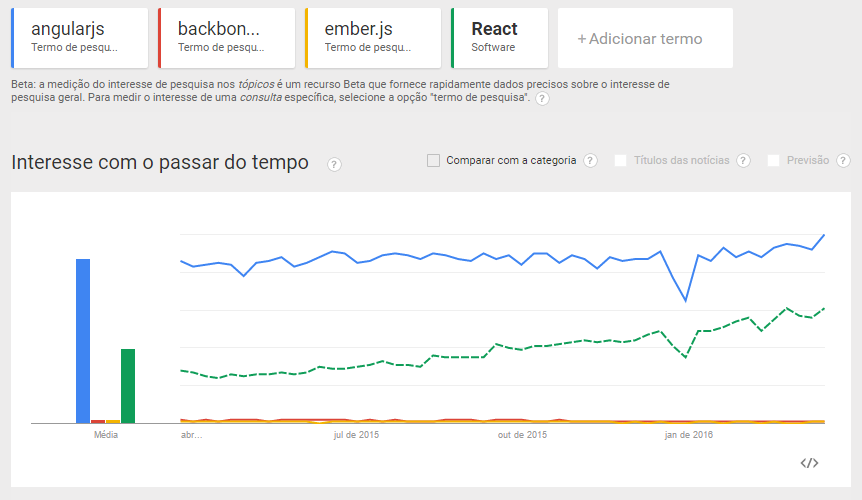
\includegraphics[width=1\textwidth]{img/grafico_ferramentas_front}
	\caption{Gráfico do Google Trends exibindo as pesquisas por ferramentas front-end}
\end{figure}


Junto ao Angular JS, será utilizada a agradável tendência de interface do Material Design da Google, que propõe layouts limpos e otimizados já conhecidos pelos usuários de smartphones Android. 


Para a elaboração da plataforma mobile do projeto, será utilizado o Ionic Framework, muito difundido e bastante pesquisado na área, o que fica evidenciado com o gráfico de pesquisbaixo, coletado via Google Trends buscando por frameworks de desenvolvimento híbrido mobile.


\begin{figure}
	\label{fig:graficoGoogleTrendsFerramentasHibridasMobile}
	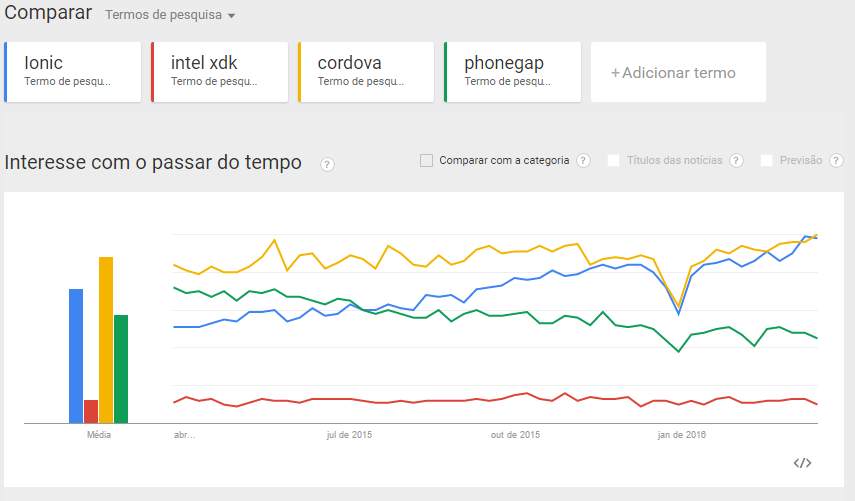
\includegraphics[width=1\textwidth]{img/grafico_ferramentas_hibridas_mobile}
	\caption{Gráfico do Google Trends exibindo as pesquisas por Frameworks híbridos mobile}
\end{figure}	

Para layout da interface mobile, também será aplicado a tendência do Material Design, a fim de propor uma harmonia entre o módulo web e mobile para os usuários


\section{Resultados Esperados}


Como fruto de um sistema para pós-graduação da UFBA, espera-se que os professores tenham mais recursos para integrar as atividades e também prover melhores condições para acompanhamento da vida acadêmica dos alunos em questão. Também, que os novos colaboradores que entrarem no processo tenham facilidade de compreender o fluxo do setor ao navegar pelo sistema proposto.


\section{Fora de Escopo}


Interação com os alunos devido às complicações para realizar a integração com o sistema empregado na UFBA, gerenciado pela XXXXXX, o que causaria uma inviabilidade no projeto devido à necessidade de entrega do produto ser mais forte que o tempo necessário para executar o processo de obtenção de acesso ao sistema legado para realizar a integração.


\section{Estrutura do Trabalho}


<breve resumo sobre os capítulos do TCC>
\chapter{Referencial Teórico}


Projetar o desenvolvimento de um software requer muito planejamento, pois as falhas iniciais podem custar bastante caro ou até mesmo inviabilizar a continuação de um projeto. Assim, a escolha da arquitetura ideal para a aplicabilidade é essencial na concepção de um produto de software. 
De todo o modo, sempre busca-se fazer mais com menos. Diante de tal filosofia, temos nesta seção, uma breve discussão sobre alguns elementos de projeto e arquitetura de software, a fim de contextualizar este trabalho de conclusão de curso.


% Ser direto no começo, focando no que realmente será discutido A seção \ref{sec:apps_mobile} 
 \section{Software como serviço}\label{sec:saas}


A definição de SaaS encontra-se muito bem elaborada em um dos trabalhos listados na literatura. Segundo La e Chun \citep{La2009Systematic}, o princípio da definição de Software como um Serviço (Sofware as a Service - SaaS) é um serviço complementar para aplicações da computação em nuvem (cloud computing). As duas áreas estão interligadas, no entanto, não se confundem, pois o SaaS deve ser entendido como um mecanismo de suporte às soluções existentes na cloud. Os SaaS existem justamente para maximizar o reuso de serviços repetidos e não centrais em uma aplicação remota.


Como propõe vantagens, software como servico é uma tendência forte, isso graças à evolução da web. Diversos fatores podem ser favoráveis para a adoção de um SaaS, como custo e manutenção dentre outros fatores aplicaveis a determinados contextos. Um trabalho recente realizado por Lechessa et al. \cite{LechesaSS11} apresenta uma pesquisa qualitativa sobre os fatores determinantes para adoção ou não de um SaaS voltado para ERP na África do Sul. Esses autores indicam que os principais fatores determinantes para adoção desse mecanismo de software são sua fluidez quanto à rede e a segurança. Esses fatores estão presentes na aplicação desenvolvida neste trabalho de conclusão de curso.
 

Devido ao fato de ter um serviço constantemente na nuvem, fica o questionamento sobre a segurança da informação manipulada. Sabe-se que a vulnerabilidade na web não é restrita ao SaaS, atingindo diversos âmbitos. O artigo de Rai et al. \cite{journals/corr/RaiSM13} orienta como o avanço da computação em nuvem não é um problema apenas para os serviços web do ponto de vista da segurança, pois muitos trabalhos na literatura mostram a área como mais um ponto de vulnerabilidade para diversos setores, a exemplo de infraestrutura. No mesmo artigo mencionado de Rai et al. \cite{journals/corr/RaiSM13}, também realizaram-se estudos exploratórios junto a empresas usuárias de serviços em computação em nuvem e consideram que a perspectiva de SaaS também pode fortalecer a segurança nas aplicações de cloud computing, pois o software de autenticação compartilhado por várias aplicações em nuvem, oferece uma melhor padronização e consequente facilidade de prevenção a erros de vulnerabilidade específicas de cada módulo da pesquisa. Esse ponto de vista é muito importante para qualquer trabalho de ponta na área de SaaS.


A arquitetura de armazenamento de dados de um Saas pode variar de acordo com a necessidade do contexto. O artigo recente de Huixin \cite{7586486}, exemplifica possíveis modelagens para utilizar. Tal abordagem pode ser com um banco de dados único, fazendo com que diferentes clientes compartilhem o mesmo banco, diferindo os dados através de controle de usuário, ou isolando os diferentes clientes através de bancos de dados exclusivos para cada um. Tal fator também pode ser combinado com a arquitetura da aplicação, caso ofereça aplicação única para todos os clientes ou aplicação compartilhada. Diante das possíveis abprdagens, a modelagem de dados do software pode ser decidida pela regra de negócio. Este trabalho optou por aplicação única e banco de dados compartilhado.


Devido ao diferente conceito de obtenção de software, tanto pela visão do cliente como pela visão do vendedor, é necessário tomar conhecimento dos diversos fatores que podem ser relevantes ao orçar um Saas. O recente trabalho de T. Kaur et al. \citep{6949281} orienta um modelo para compor o custo de um Saas. O custo total seria composto pelos fatores que dão suporte ao funcionamento do software. Tais fatores incluem infra-estrutura, configurabilidade, customização, parâmetros de QoS(Quality of service) como escalabilidade, disponibilidade, usabilidade, pontualidade e desempenho da resposta, portabilidade, custo total de propriedade e retorno do investimento. Esses fatores caracterizam o custo de forma eficaz, possibilitando ao fornecedor, prover um Serviço de acordo com a exigência do consumidor em vários pacotes de serviços.


\section{Reuso de software}\label{sec:reuso} %CRUISE BOOK CAPITULO 2


Para Peter Freeman, o reuso é a utilização de qualquer informação que um desenvolvedor pode necessitar no processo de criação de software (Ezran et al., 2002). Basili e Rombach definem reutilização de software como o uso de tudo o que está associado a um projeto de conhecimento (Basili e Rombach, 1991).
Assim, o objetivo da reutilização de software é reciclar o design, código e outros componentes de um produto de software e assim reduzir o custo, o tempo e melhorar a qualidade do produto.
Segundo Keswani et al. \cite{6783445}, o componente reutilizável de software pode ser qualquer parte de seu desenvolvimento, como um fragmento de código, design, casos de teste, ou até mesmo a especificação de requisitos de uma funcionalidade do software. 

O reuso de software pode ter impacto positivo em diversos aspectos do software, vejamos alguns, conforme apresentados no C.R.U.I.S.E Book:

\begin{itemize}

\item Qualidade: As correções de erro tornam-se úteis em todos os locais em que ocorreu, padronizando e facilitando a manutenção.

\item Produtividade: O ganho de produtividade é alcançado devido ao menor número de artefatos desenvolvido. Isso resulta em menos esforços de teste e também economiza análise e design, gerando economia em diversos escopos do projeto.

\item Confiabilidade: A utilização de componentes bem testados aumenta a
confiança no software. Além disso, a utilização de um mesmo componente em vários sistemas, aumenta a possibilidade de detecção de erros e reforça a confiança no componente.

\item Redução do Esforço: A reutilização de software proporciona uma redução do tempo de desenvolvimento, o que reduz o tempo necessário para o produto ser disponibilizado no mercado para trazer rentabilidade.

\item Trabalho redundante e tempo de desenvolvimento: Desenvolver um sistema do
zero significa desenvolvimento redundante de muitos componentes, como requisito
especificações, casos de uso, arquitetura, etc. Isso pode ser evitado quando estes estão disponíveis como componentes reutilizáveis e podem ser compartilhados, resultando em menos desenvolvimento, tempo e custo associado.

\item Documentação: Embora a documentação seja muito importante para a
manutenção de um sistema, muitas vezes é negligenciada. A reutilização de componentes software reduz a quantidade de documentação a ser escrita, entretanto depende da qualidade do que está escrito. Assim, apenas a estrutura do sistema e os novos artefatos desenvolvidos necessitam ser documentados.

\item Custo de manutenção: Menos defeitos e manutenções são esperados quando tem-se comprovada a qualidade dos componentes utilizados.

\item Tamanho da equipe: É comum entrar casos em que a equipe de desenvolvimento sofre sobrecarga. Entretanto, dobrar o tamanho da equipe de desenvolvimento não necessariamente duplica produtividade. Se muitos componentes podem ser reutilizados, é possível desenvolver com equipes menores, levando a melhores comunicações e aumento da produtividade.

\end{itemize}

Apesar dos benefícios da reutilização de software, a mesma não é amplamente praticado como imagina-se. Existem fatores que influenciam direta ou indiretamente na sua adoção. Esses fatores podem ser de aspecto gerencial, organizacional, econômico, conceitual ou técnico. Veremos a seguir alguns aspectos que podem gerar conflito com a cultura de reuso de software, segundo o C.R.U.I.S.E Book:
%(Sametinger, 1997). REVER

\begin{itemize}
	
\item Falta de apoio da gestão: Como a reutilização de software gera custos iniciais,
a medida pode não ser amplamente alcançada em uma organização sem o apoio de alto nível gestão. Os gestores têm de ser informados sobre os custos iniciais e serem convencidos sobre economias futuras.

\item Gerenciamento do Projeto: Gerenciar projetos tradicionais é uma tarefa árdua, principalmente, os que praticam a reutilização de software. Utilizando a técnica em larga escala, tem-se impacto sobre todo o ciclo de vida do software.

\item Estruturas organizacionais inadequadas: As estruturas organizacionais devem
considerar diferentes necessidades que surgem quando a reutilização em larga escala está sendo adotada. Por exemplo, uma equipe particionada pode ser alocada somente para desenvolver, manter e certificar componentes reutilizáveis de software.

\item Incentivos de gestão: É comum a falta de incentivo para deixar os desenvolvedores gastarem tempo elaborando reutilizáveis componentes do sistema. A produtividade é muitas vezes medida apenas no tempo necessário para concluir um projeto. Assim, fazer qualquer trabalho além disso, embora benéfico para a empresa como um todo, diminui o seu sucesso. Mesmo quando os componentes reutilizáveis são utilizados, os benefícios obtidos são uma pequena fração do que poderia ser alcançado caso houvesse reutilização explícita, planejada e organizada.

\item Dificuldade de encontrar software reutilizável: Para reutilizar os componentes, devem existir formas eficientes de busca. Além disso, é importante ter um repositório bem organizado contendo componentes com um eficiente meio de acesso.

\item Não reutilização do software encontrado. O acesso fácil ao software existente
não necessariamente aumentar a reutilização. Os componentes reutilizáveis devem ser cuidadosamente especificados, projetados, implementados e documentados, pois em alguns casos, modificar e adaptar o código  pode ser mais custoso que a programação da funcionalidade necessária a partir do zero.

\item Modificação: É muito difícil encontrar um componente que funcione
exatamente da mesma maneira que queremos. Desta forma, são necessárias modificações e devem existir formas de determinar os seus efeitos sobre o componente.


\end{itemize}


%Outra diretriz importante para a reutilização de software é reduzir o risco na criação de novos softwares. O risco tende a ser bastante reduzido se os componentes que estão sendo reutilizados têm as documentação, interfaces necessárias e devidamente testadas, fatores que contibruem para uma fácil integração.
%De acordo com Keswani et al. \citep{6783445}, para o reuso de software dar retornos apropriados, o processo deve ser sistemático e planejado. Qualquer organização que implemente a reutilização de software deve identificar os melhores métodos e estratégias de reutilização para obter a máxima produtividade. A reutilização de software ajuda a evitar software de engenharia a partir do zero, pois usa módulos de software existentes. A reutilização de software, embora seja uma tarefa difícil, especialmente para softwares antigos sem padrões de projeto, pode melhorar significativamente a produtividade e a qualidade de um produto de software. Embora a reutilização de software não seja um novo campo, ela pode dar grandes retornos em curto período de tempo.


\section{Modularização}\label{sec:modularizacao} %artigo de claudio pagina 222 introdução


%A modularidade vem desempenhando um papel predominante estágios emergentes das disciplinas de arquitetura de software [13]. Engenheiros de software consideram modularidade como princípio base na comparação entre arquiteturas alternativas  e arquitetura degeneração [9]. De fato, os engenheiros de software são incentivados a arquitecturas, baseando-se numa multiplicidade de mecanismos de modularidade disponíveis em: 
%(i) Linguagens de descrição de arquitetura (ADLs), como ACME [8], 
%(ii) catálogos de arquitetônicos [2, 13], e 
%(iii) conhecem bem princípios de alto nível, como interfaces de componentes estreitos, acoplamento arquitectónico reduzido e semelhantes.


Conforme é frisado no trabalho de Wickramaarachchi e Lai \citep{7062705}, o conceito de modularização na indústria de software tem uma longa história e tem sido utilizado para melhorar o processo de desenvolvimento de software em diferentes estágios. Os principais conceitos por trás da modularização do software foram introduzidos por pesquisadores pioneiros há quarenta anos, com uma notável contribuição feita por Melvin Conway e David Parnas, que tem representação notável na engenharia de software.


Modularizar um software é um bom padrão a ser adotado. Segundo Wickramaarachchi e Lai \citep{7062705}, a modularização é importante na identificação de dependências e reduz as dificuldades diante de uma possível necessidade de grandes alterações. De uma perspectiva da engenharia de software, uma modularização geralmente tem várias vantagens, tais como: tornar a complexidade do software mais gerenciável, facilitar o trabalho paralelo e tornar o software mais maleável para acomodar o futuro incerto que um software pode ter. O objetivo final da modularização do software é aumentar a produtividade ea qualidade do software. Tal conceito encontra-se bastante difundido e estái incorporado em linguagens de programação e ferramentas de software. O trabalho proposto favorece ao uso da modularização de um software e até mesmo pode ser considerado um módulo a ser acoplado a qualquer software, mediante a compatibilidade.


\section{Aplicações web}\label{sec:apps_web}


A popularidade da aplicação web aumentou exponencialmente na última década e todos os dias cresce o número de pessoas usuárias de aplicações web. E seguindo o padrão de desenvolvimento de software, Kumar et al. \citep{7813710} sugerem que para o desenvolvimento web, deve-se manter a prática efiacaz de produzir diagramas UML. A abordagem baseada na web oferece uma maneira fácil e eficaz para gerenciar e controlar o processo de desenvolvimento por meio de diagramas UML. Tal abordagem pode ser usada quando há uma exigência de lidar com mudanças muito rápidas e grandes em requisitos de forma muito eficaz em muito menos tempo, gerando assim um menor impacto. 


Para atender à fomentada demanda de aplicativos web, é necessário adotar métodos de desenvolvimentos que sejam ágeis, eficientes e de fácil manutenção. Yu Ping et al. \cite{1372143} propõem o uso do modelo MVC (Model, View e Controller) no atual desenvolvimento para softwares web. O modelo apresentado tornou-se um padrão popular e divide o software em camadas com propósito definido, tornando-o de mais fácil manutenção.


O Ajax (Asynchronous Javascript and XML) revolucionou a web. Conforme demonstrado no artigo de Yuping \citep{6845605}, ao usar a tecnologia Ajax, podemos enriquecer a experiência do usuário em aplicações baseadas em navegador de internet, e fornecer uma variedade de aplicações interativas para atender às necessidade de humanização das aplicações.
Os aplicativos Ajax em execução no navegador se comunicam com um servidor Web de forma assíncrona e atualizam apenas uma parte da página.



% %% RiSE Latex Template - version 0.5
%%
%% RiSE's latex template for thesis and dissertations
%% http://risetemplate.sourceforge.net
%%
%% (c) 2012 Yguaratã Cerqueira Cavalcanti (yguarata@gmail.com)
%%          Vinicius Cardoso Garcia (vinicius.garcia@gmail.com)
%%
%% This document was initially based on UFPEThesis template, from Paulo Gustavo
%% S. Fonseca.
%%
%% ACKNOWLEDGEMENTS
%%
%% We would like to thanks the RiSE's researchers community, the 
%% students from Federal University of Pernambuco, and other users that have
%% been contributing to this projects with comments and patches.
%%
%% GENERAL INSTRUCTIONS
%%
%% We strongly recommend you to compile your documents using pdflatex command.
%% It is also recommend use the texlipse plugin for Eclipse to edit your documents.
%%
%% Options for \documentclass command:
%%         * Idiom
%%           pt   - Portguese (default)
%%           en   - English
%%
%%         * Text type
%%           bsc  - B.Sc. Thesis
%%           msc  - M.Sc. Thesis (default)
%%           qual - PHD qualification (not tested yet)
%%           prop - PHD proposal (not tested yet)
%%           phd  - PHD thesis
%%
%%         * Media
%%           scr  - to eletronic version (PDF) / see the users guide
%%
%%         * Pagination
%%           oneside - unique face press
%%           twoside - two faces press
%%
%%		   * Line spacing
%%           singlespacing  - the same as using \linespread{1}
%%           onehalfspacing - the same as using \linespread{1.3}
%%           doublespacing  - the same as using \linespread{1.6}
%%
%% Reference commands. Use the following commands to make references in your
%% text:
%%          \figref  -- for Figure reference
%%          \tabref  -- for Table reference
%%          \eqnref  -- for equation reference
%%          \chapref -- for chapter reference
%%          \secref  -- for section reference
%%          \appref  -- for appendix reference
%%          \axiref  -- for axiom reference
%%          \conjref -- for conjecture reference
%%          \defref  -- for definition reference
%%          \lemref  -- for lemma reference
%%          \theoref -- for theorem reference
%%          \corref  -- for corollary reference
%%          \propref -- for proprosition reference
%%          \pgref   -- for page reference
%%
%%          Example: See \chapref{chap:introduction}. It will produce 
%%                   'See Chapter 1', in case of English language.

\documentclass[pt,twoside,onehalfspacing,bsc]{risethesis}

\usepackage[utf8]{inputenc}
\usepackage[brazilian]{babel}
\usepackage[T1]{fontenc}

%% Change the following pdf author attribute name to your name.
\usepackage[linkcolor=blue,citecolor=blue,urlcolor=blue,colorlinks,pdfpagelabels,pdftitle={Bruno Cabral's Bachelor Thesis},pdfauthor={Bruno Cabral}]{hyperref}

\address{SALVADOR}

\universitypt{Universidade Federal da Bahia}
\universityen{Federal University of Bahia}

\departmentpt{Depertamento de Ciência da Computação}
\departmenten{Computer Science Department}

\programpt{Programa Multiinstitucional de Pós-graduação em Ciência da Computação}
\programen{Graduate in Computer Science}

\majorfieldpt{Ciência da Computação}
\majorfielden{Computer Science}

\title{Sistema de apoio à Pós graduação - UFBA}
\date{Outubro/2016}

\author{Victor de Azevedo Nunes}
\adviser{Ivan do Carmo Machado}

\begin{document}

\frontmatter
\frontpage
\presentationpage

\begin{dedicatory}
Eu dedico esta dissertação...
%I dedicate this dissertation to my family, girlfriend, friends and
%professors who gave me all necessary support to get here.
\end{dedicatory}

\acknowledgements
Meus agradecimentos...

\begin{epigraph}[]{Edward V Berard}
Walking on water and developing software from a specification are easy if both are frozen
\end{epigraph}

\resumo
% Escreva seu resumo no arquivo resumo.tex
Meu resumo

\begin{keywords}
palavras chave

\end{keywords}

\abstract
% Write your abstract in a file called abstract.tex
My abstract...

\begin{keywords}
key words...
\end{keywords}

% Summary (tables of contents)
\tableofcontents

% List of figures
\listoffigures

% List of tables
\listoftables

% List of acronyms
% Acronyms manual: http://linorg.usp.br/CTAN/macros/latex/contrib/acronym/acronym.pdf
\listofacronyms
\begin{acronym}[ACRONYM] 
% Change the word ACRONYM above to change the acronym column width.
% The column width is equals to the width of the word that you put.
% Read the manual about acronym package for more examples:
%   http://linorg.usp.br/CTAN/macros/latex/contrib/acronym/acronym.pdf

\acro{SPA}{Single Page Application}
\acro{JSON}{Javascript Object Notation}
\acro{PHP}{PHP: Hypertext Preprocessor}
\acro{SaaS}{Software as a Service}
\acro{ERP}{Enterprise Resource Planning}
\acro{QoS}{Quality of Service}
\acro{UML}{Unified Modeling Language}
\acro{MVC}{Model-View-Controller}
\acro{Ajax}{Asynchronous Javascript and XML}
\acro{HTML}{HyperText Markup Language}
\acro{CSS}{Cascading Style Sheets}
\acro{API}{Application Programming Interface}
\acro{DOM}{Document Object Model}
\acro{BPMN}{Business Process Model and Notation}
\acro{REST}{Representational State Transfer}

\end{acronym}

% List of listings
%\lstlistoflistings

\mainmatter

\chapter{Introdução}

\section{Motivação}

Organizar os procedimentos de um processo sempre nos traz vantagens. Apesar de no processo de implantação de um sistema, o mesmo burocratizar o processo, com o tempo temos o retorno da dedicação para a inserção dos dados. Com um certo volume de dados, é possível estruturar informações que num processo manual são difíceis de serem enxergadas. Assim, é possível depender menos das pessoas que organizam o processo, pois o legado de informações não estará mais somente na mente de alguns, mas sim documentado nos dados do sistema.

Além de colaborar na organização, também haverá uma grande colaboração no tempo gasto na gestão. Lidar com muitos papéis e confiar na mente humana para guardar informações, não é uma alternativa muito segura devido ao fato que as pessoas sempre estão sujeitas a sair do processo e levar contigo a experiência obtida. Experiência essa que faz com que os procedimentos sejam executados de forma mais eficiente. Entretanto, com um sistema inteligente, é possível auxiliar e tornar mais ágil a execução das tarefas.


\section{Problema}


De acordo com funcionários ligados ao o setor de pós graduação da UFBA, entrevistados a fim de um maior entendimento do cenário, apesar das semelhanças estruturais, a pós graduação gerida de forma diferencia da graduação. FULANO afirma que devido ao fato de não ter a mesma visibilidade, não tem acesso aos mesmos recursos de gestão acadêmica da graduação. O professores não executam somente atividades dentro da sala de aula, também tem diversas outras ocupações no setor. E muitos procedimentos realizados extra classe ainda se encontram sendo realizados de forma manual, estando mais vulnerável ao erro ou até mesmo à violação do processo. Também ocorre um grande desperdício de tempo pelos professores e gestores da área, devido ao diversos processos ainda realizados de forma manual, sem a devida documentação. Segundo FULANO, também entrevistado, esse tempo perdido implica numa redução da eficiência na sala de aula, pois o professor acaba por ter menos tempo disponível para o planejamento das atividades, o que gera impactos negativos aos alunos.


\section{Objetivos} %<o que deve ser feito/entregue>


Devido aos muitos processos sendo resolvidos de forma manual, propõe-se com solução um sistema moderno, arquitetado para ter funcionamento na web e com um módulo mobile, a fim de fornecer informações de forma rápida e eficiente para os professores através de notificações, já que o acesso à internet móvel é comum entre os possíveis usuários do sistema em questão.
O principal requisito para o sistema seria dispor recursos para reduzir o tempo desperdiçado pelos professores durante as atividades extra classe.


\section{Metodologia} %<como será feito | como resolver o problema apontado inicialmente>


%<analise de literatura | design | implementação | validação>
Baseando-se nas tecnologias gratuitas em alta no cenário atual do desenvolvimento web, dispomos de algumas opções eficientes para a implementação da solução. Dentre as possibilidades, considerando a facilidade para futura manutenção e continuidade do projeto, tende-se a optar por uma tecnologia popular. Como linguagem de programação, adota-se o PHP. A escolha é fundamentada de acordo com a pesquisa da RedMonk de 2015, que evidencia o uso das linguagens de programação de acordo com as discussões no StackOverflow e repositórios no GitHub. É possível constatar a popularidade do PHP no cenário atual com o gráfico da pesquisa citada, na qual o PHP é apresentado na terceira colocação, apenas atrás do lider JavaScript e do segundo colocado, o Java.

\begin{figure}
	\label{fig:graficoRedmonk}
	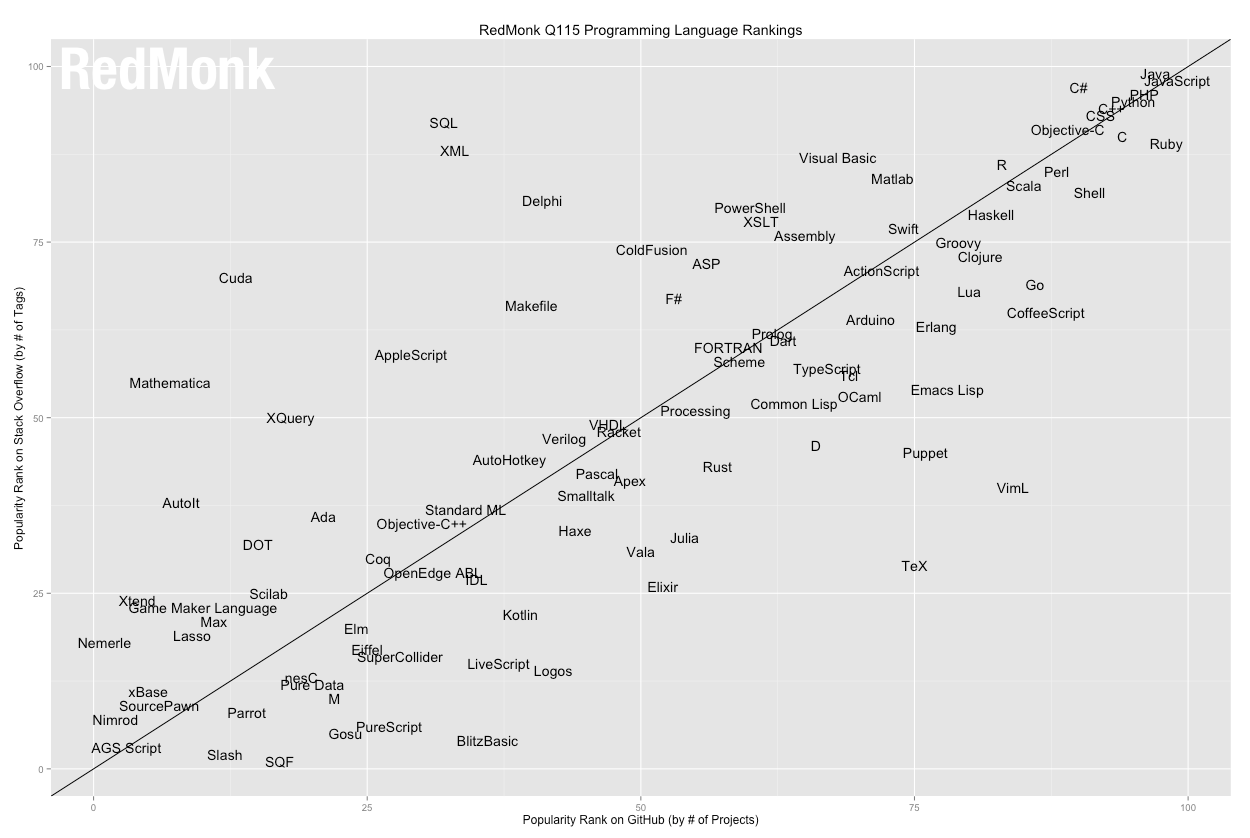
\includegraphics[width=1\textwidth]{img/grafico_redmonk}
	\caption{Ranking das liguagens de programação no Stack Overflow e Github}
\end{figure}


Ainda assim, para compor a interface do dado projeto, também ocorrerá o uso do líder JavaScript de forma intensa, provendo o elo com o as informações gerenciadas pelo PHP.


Entretanto, não seria inteligente desenvolver um sistema completo sem o auxílio de um framework. Dentre os frameworks disponíveis para PHP, hoje o destaque está com o Laravel, que se encontra no topo dentre os mais utilizados no momento. 


A WebHostFace, uma empresa de hospedagem, compilou várias estatísticas para criar um infográfico mostrando os frameworks PHP mais populares de 2015. Utilizando informações sobre os próprios clientes, o Google Trends, estatísticas de repositórios do GitHub e a pesquisa do SitePoint “Best PHP Frameworks 2015”, a WebHostFace elaborou o seguinte infográfico: 

\begin{figure}
	\label{fig:graficoWebhostface}
	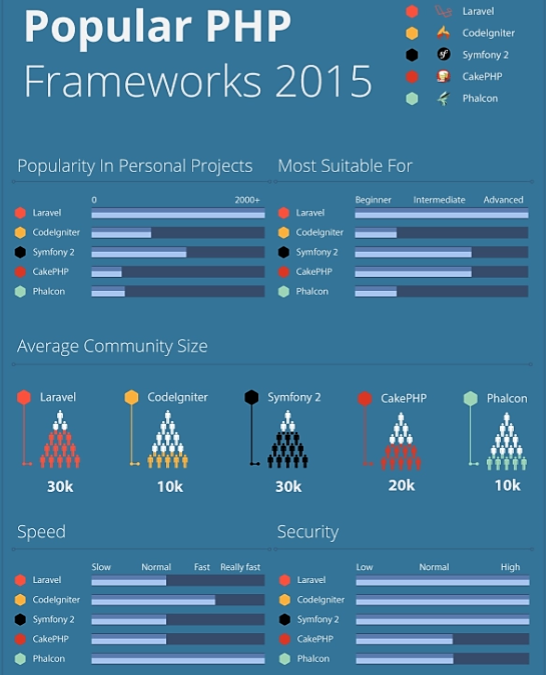
\includegraphics[width=1\textwidth]{img/infografico_webhostface}
	\caption{Infográfico da WebhostFace, exibindo a popularidade dos Frameworks PHP em 2015}
\end{figure}

Assim, tem-se a evidência que o Laravel em 2015 teve a maior popularidade em projetos pessoais e tem a maior comunidade entre os concorrentes, o que o torna uma boa escolha para a escrita de um software que será continuado por terceiros.


Para elaborar os recursos de interface e integrar ao back-end PHP do sistema, será adotado o já conhecido AngularJS, ferramenta sólida e conhecida no aspecto em questão. 


Dados coletados via Google Trends, que propõe comparações entre termos pesquisados, revela a popularidade do AngularJs diante de alguns dos principais concorrentes. O gráfico abaixo evidencia o cenário.


%Como mostra a Figura \ref{fig:graficoGoogleTrendsFerramentasFront}. 
\begin{figure}
	\label{fig:graficoGoogleTrendsFerramentasFront}
	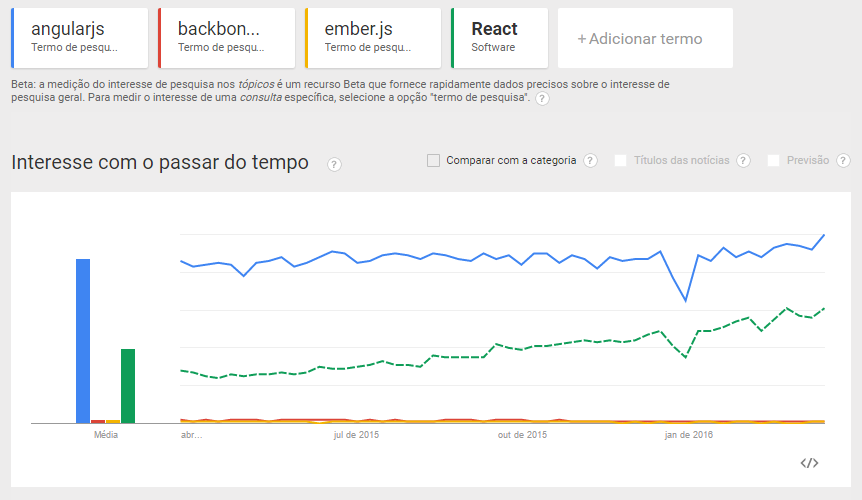
\includegraphics[width=1\textwidth]{img/grafico_ferramentas_front}
	\caption{Gráfico do Google Trends exibindo as pesquisas por ferramentas front-end}
\end{figure}


Junto ao Angular JS, será utilizada a agradável tendência de interface do Material Design da Google, que propõe layouts limpos e otimizados já conhecidos pelos usuários de smartphones Android. 


Para a elaboração da plataforma mobile do projeto, será utilizado o Ionic Framework, muito difundido e bastante pesquisado na área, o que fica evidenciado com o gráfico de pesquisbaixo, coletado via Google Trends buscando por frameworks de desenvolvimento híbrido mobile.


\begin{figure}
	\label{fig:graficoGoogleTrendsFerramentasHibridasMobile}
	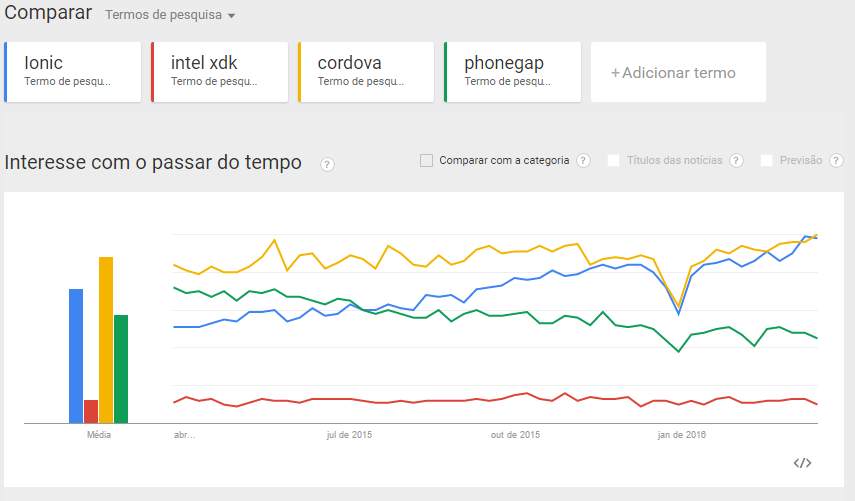
\includegraphics[width=1\textwidth]{img/grafico_ferramentas_hibridas_mobile}
	\caption{Gráfico do Google Trends exibindo as pesquisas por Frameworks híbridos mobile}
\end{figure}	

Para layout da interface mobile, também será aplicado a tendência do Material Design, a fim de propor uma harmonia entre o módulo web e mobile para os usuários


\section{Resultados Esperados}


Como fruto de um sistema para pós-graduação da UFBA, espera-se que os professores tenham mais recursos para integrar as atividades e também prover melhores condições para acompanhamento da vida acadêmica dos alunos em questão. Também, que os novos colaboradores que entrarem no processo tenham facilidade de compreender o fluxo do setor ao navegar pelo sistema proposto.


\section{Fora de Escopo}


Interação com os alunos devido às complicações para realizar a integração com o sistema empregado na UFBA, gerenciado pela XXXXXX, o que causaria uma inviabilidade no projeto devido à necessidade de entrega do produto ser mais forte que o tempo necessário para executar o processo de obtenção de acesso ao sistema legado para realizar a integração.


\section{Estrutura do Trabalho}


<breve resumo sobre os capítulos do TCC>
\chapter{Referencial Teórico}


Projetar o desenvolvimento de um software requer muito planejamento, pois as falhas iniciais podem custar bastante caro ou até mesmo inviabilizar a continuação de um projeto. Assim, a escolha da arquitetura ideal para a aplicabilidade é essencial na concepção de um produto de software. 
De todo o modo, sempre busca-se fazer mais com menos. Diante de tal filosofia, temos nesta seção, uma breve discussão sobre alguns elementos de projeto e arquitetura de software, a fim de contextualizar este trabalho de conclusão de curso.


% Ser direto no começo, focando no que realmente será discutido A seção \ref{sec:apps_mobile} 
 \section{Software como serviço}\label{sec:saas}


A definição de SaaS encontra-se muito bem elaborada em um dos trabalhos listados na literatura. Segundo La e Chun \citep{La2009Systematic}, o princípio da definição de Software como um Serviço (Sofware as a Service - SaaS) é um serviço complementar para aplicações da computação em nuvem (cloud computing). As duas áreas estão interligadas, no entanto, não se confundem, pois o SaaS deve ser entendido como um mecanismo de suporte às soluções existentes na cloud. Os SaaS existem justamente para maximizar o reuso de serviços repetidos e não centrais em uma aplicação remota.


Como propõe vantagens, software como servico é uma tendência forte, isso graças à evolução da web. Diversos fatores podem ser favoráveis para a adoção de um SaaS, como custo e manutenção dentre outros fatores aplicaveis a determinados contextos. Um trabalho recente realizado por Lechessa et al. \cite{LechesaSS11} apresenta uma pesquisa qualitativa sobre os fatores determinantes para adoção ou não de um SaaS voltado para ERP na África do Sul. Esses autores indicam que os principais fatores determinantes para adoção desse mecanismo de software são sua fluidez quanto à rede e a segurança. Esses fatores estão presentes na aplicação desenvolvida neste trabalho de conclusão de curso.
 

Devido ao fato de ter um serviço constantemente na nuvem, fica o questionamento sobre a segurança da informação manipulada. Sabe-se que a vulnerabilidade na web não é restrita ao SaaS, atingindo diversos âmbitos. O artigo de Rai et al. \cite{journals/corr/RaiSM13} orienta como o avanço da computação em nuvem não é um problema apenas para os serviços web do ponto de vista da segurança, pois muitos trabalhos na literatura mostram a área como mais um ponto de vulnerabilidade para diversos setores, a exemplo de infraestrutura. No mesmo artigo mencionado de Rai et al. \cite{journals/corr/RaiSM13}, também realizaram-se estudos exploratórios junto a empresas usuárias de serviços em computação em nuvem e consideram que a perspectiva de SaaS também pode fortalecer a segurança nas aplicações de cloud computing, pois o software de autenticação compartilhado por várias aplicações em nuvem, oferece uma melhor padronização e consequente facilidade de prevenção a erros de vulnerabilidade específicas de cada módulo da pesquisa. Esse ponto de vista é muito importante para qualquer trabalho de ponta na área de SaaS.


A arquitetura de armazenamento de dados de um Saas pode variar de acordo com a necessidade do contexto. O artigo recente de Huixin \cite{7586486}, exemplifica possíveis modelagens para utilizar. Tal abordagem pode ser com um banco de dados único, fazendo com que diferentes clientes compartilhem o mesmo banco, diferindo os dados através de controle de usuário, ou isolando os diferentes clientes através de bancos de dados exclusivos para cada um. Tal fator também pode ser combinado com a arquitetura da aplicação, caso ofereça aplicação única para todos os clientes ou aplicação compartilhada. Diante das possíveis abprdagens, a modelagem de dados do software pode ser decidida pela regra de negócio. Este trabalho optou por aplicação única e banco de dados compartilhado.


Devido ao diferente conceito de obtenção de software, tanto pela visão do cliente como pela visão do vendedor, é necessário tomar conhecimento dos diversos fatores que podem ser relevantes ao orçar um Saas. O recente trabalho de T. Kaur et al. \citep{6949281} orienta um modelo para compor o custo de um Saas. O custo total seria composto pelos fatores que dão suporte ao funcionamento do software. Tais fatores incluem infra-estrutura, configurabilidade, customização, parâmetros de QoS(Quality of service) como escalabilidade, disponibilidade, usabilidade, pontualidade e desempenho da resposta, portabilidade, custo total de propriedade e retorno do investimento. Esses fatores caracterizam o custo de forma eficaz, possibilitando ao fornecedor, prover um Serviço de acordo com a exigência do consumidor em vários pacotes de serviços.


\section{Reuso de software}\label{sec:reuso} %CRUISE BOOK CAPITULO 2


Para Peter Freeman, o reuso é a utilização de qualquer informação que um desenvolvedor pode necessitar no processo de criação de software (Ezran et al., 2002). Basili e Rombach definem reutilização de software como o uso de tudo o que está associado a um projeto de conhecimento (Basili e Rombach, 1991).
Assim, o objetivo da reutilização de software é reciclar o design, código e outros componentes de um produto de software e assim reduzir o custo, o tempo e melhorar a qualidade do produto.
Segundo Keswani et al. \cite{6783445}, o componente reutilizável de software pode ser qualquer parte de seu desenvolvimento, como um fragmento de código, design, casos de teste, ou até mesmo a especificação de requisitos de uma funcionalidade do software. 

O reuso de software pode ter impacto positivo em diversos aspectos do software, vejamos alguns, conforme apresentados no C.R.U.I.S.E Book:

\begin{itemize}

\item Qualidade: As correções de erro tornam-se úteis em todos os locais em que ocorreu, padronizando e facilitando a manutenção.

\item Produtividade: O ganho de produtividade é alcançado devido ao menor número de artefatos desenvolvido. Isso resulta em menos esforços de teste e também economiza análise e design, gerando economia em diversos escopos do projeto.

\item Confiabilidade: A utilização de componentes bem testados aumenta a
confiança no software. Além disso, a utilização de um mesmo componente em vários sistemas, aumenta a possibilidade de detecção de erros e reforça a confiança no componente.

\item Redução do Esforço: A reutilização de software proporciona uma redução do tempo de desenvolvimento, o que reduz o tempo necessário para o produto ser disponibilizado no mercado para trazer rentabilidade.

\item Trabalho redundante e tempo de desenvolvimento: Desenvolver um sistema do
zero significa desenvolvimento redundante de muitos componentes, como requisito
especificações, casos de uso, arquitetura, etc. Isso pode ser evitado quando estes estão disponíveis como componentes reutilizáveis e podem ser compartilhados, resultando em menos desenvolvimento, tempo e custo associado.

\item Documentação: Embora a documentação seja muito importante para a
manutenção de um sistema, muitas vezes é negligenciada. A reutilização de componentes software reduz a quantidade de documentação a ser escrita, entretanto depende da qualidade do que está escrito. Assim, apenas a estrutura do sistema e os novos artefatos desenvolvidos necessitam ser documentados.

\item Custo de manutenção: Menos defeitos e manutenções são esperados quando tem-se comprovada a qualidade dos componentes utilizados.

\item Tamanho da equipe: É comum entrar casos em que a equipe de desenvolvimento sofre sobrecarga. Entretanto, dobrar o tamanho da equipe de desenvolvimento não necessariamente duplica produtividade. Se muitos componentes podem ser reutilizados, é possível desenvolver com equipes menores, levando a melhores comunicações e aumento da produtividade.

\end{itemize}

Apesar dos benefícios da reutilização de software, a mesma não é amplamente praticado como imagina-se. Existem fatores que influenciam direta ou indiretamente na sua adoção. Esses fatores podem ser de aspecto gerencial, organizacional, econômico, conceitual ou técnico. Veremos a seguir alguns aspectos que podem gerar conflito com a cultura de reuso de software, segundo o C.R.U.I.S.E Book:
%(Sametinger, 1997). REVER

\begin{itemize}
	
\item Falta de apoio da gestão: Como a reutilização de software gera custos iniciais,
a medida pode não ser amplamente alcançada em uma organização sem o apoio de alto nível gestão. Os gestores têm de ser informados sobre os custos iniciais e serem convencidos sobre economias futuras.

\item Gerenciamento do Projeto: Gerenciar projetos tradicionais é uma tarefa árdua, principalmente, os que praticam a reutilização de software. Utilizando a técnica em larga escala, tem-se impacto sobre todo o ciclo de vida do software.

\item Estruturas organizacionais inadequadas: As estruturas organizacionais devem
considerar diferentes necessidades que surgem quando a reutilização em larga escala está sendo adotada. Por exemplo, uma equipe particionada pode ser alocada somente para desenvolver, manter e certificar componentes reutilizáveis de software.

\item Incentivos de gestão: É comum a falta de incentivo para deixar os desenvolvedores gastarem tempo elaborando reutilizáveis componentes do sistema. A produtividade é muitas vezes medida apenas no tempo necessário para concluir um projeto. Assim, fazer qualquer trabalho além disso, embora benéfico para a empresa como um todo, diminui o seu sucesso. Mesmo quando os componentes reutilizáveis são utilizados, os benefícios obtidos são uma pequena fração do que poderia ser alcançado caso houvesse reutilização explícita, planejada e organizada.

\item Dificuldade de encontrar software reutilizável: Para reutilizar os componentes, devem existir formas eficientes de busca. Além disso, é importante ter um repositório bem organizado contendo componentes com um eficiente meio de acesso.

\item Não reutilização do software encontrado. O acesso fácil ao software existente
não necessariamente aumentar a reutilização. Os componentes reutilizáveis devem ser cuidadosamente especificados, projetados, implementados e documentados, pois em alguns casos, modificar e adaptar o código  pode ser mais custoso que a programação da funcionalidade necessária a partir do zero.

\item Modificação: É muito difícil encontrar um componente que funcione
exatamente da mesma maneira que queremos. Desta forma, são necessárias modificações e devem existir formas de determinar os seus efeitos sobre o componente.


\end{itemize}


%Outra diretriz importante para a reutilização de software é reduzir o risco na criação de novos softwares. O risco tende a ser bastante reduzido se os componentes que estão sendo reutilizados têm as documentação, interfaces necessárias e devidamente testadas, fatores que contibruem para uma fácil integração.
%De acordo com Keswani et al. \citep{6783445}, para o reuso de software dar retornos apropriados, o processo deve ser sistemático e planejado. Qualquer organização que implemente a reutilização de software deve identificar os melhores métodos e estratégias de reutilização para obter a máxima produtividade. A reutilização de software ajuda a evitar software de engenharia a partir do zero, pois usa módulos de software existentes. A reutilização de software, embora seja uma tarefa difícil, especialmente para softwares antigos sem padrões de projeto, pode melhorar significativamente a produtividade e a qualidade de um produto de software. Embora a reutilização de software não seja um novo campo, ela pode dar grandes retornos em curto período de tempo.


\section{Modularização}\label{sec:modularizacao} %artigo de claudio pagina 222 introdução


%A modularidade vem desempenhando um papel predominante estágios emergentes das disciplinas de arquitetura de software [13]. Engenheiros de software consideram modularidade como princípio base na comparação entre arquiteturas alternativas  e arquitetura degeneração [9]. De fato, os engenheiros de software são incentivados a arquitecturas, baseando-se numa multiplicidade de mecanismos de modularidade disponíveis em: 
%(i) Linguagens de descrição de arquitetura (ADLs), como ACME [8], 
%(ii) catálogos de arquitetônicos [2, 13], e 
%(iii) conhecem bem princípios de alto nível, como interfaces de componentes estreitos, acoplamento arquitectónico reduzido e semelhantes.


Conforme é frisado no trabalho de Wickramaarachchi e Lai \citep{7062705}, o conceito de modularização na indústria de software tem uma longa história e tem sido utilizado para melhorar o processo de desenvolvimento de software em diferentes estágios. Os principais conceitos por trás da modularização do software foram introduzidos por pesquisadores pioneiros há quarenta anos, com uma notável contribuição feita por Melvin Conway e David Parnas, que tem representação notável na engenharia de software.


Modularizar um software é um bom padrão a ser adotado. Segundo Wickramaarachchi e Lai \citep{7062705}, a modularização é importante na identificação de dependências e reduz as dificuldades diante de uma possível necessidade de grandes alterações. De uma perspectiva da engenharia de software, uma modularização geralmente tem várias vantagens, tais como: tornar a complexidade do software mais gerenciável, facilitar o trabalho paralelo e tornar o software mais maleável para acomodar o futuro incerto que um software pode ter. O objetivo final da modularização do software é aumentar a produtividade ea qualidade do software. Tal conceito encontra-se bastante difundido e estái incorporado em linguagens de programação e ferramentas de software. O trabalho proposto favorece ao uso da modularização de um software e até mesmo pode ser considerado um módulo a ser acoplado a qualquer software, mediante a compatibilidade.


\section{Aplicações web}\label{sec:apps_web}


A popularidade da aplicação web aumentou exponencialmente na última década e todos os dias cresce o número de pessoas usuárias de aplicações web. E seguindo o padrão de desenvolvimento de software, Kumar et al. \citep{7813710} sugerem que para o desenvolvimento web, deve-se manter a prática efiacaz de produzir diagramas UML. A abordagem baseada na web oferece uma maneira fácil e eficaz para gerenciar e controlar o processo de desenvolvimento por meio de diagramas UML. Tal abordagem pode ser usada quando há uma exigência de lidar com mudanças muito rápidas e grandes em requisitos de forma muito eficaz em muito menos tempo, gerando assim um menor impacto. 


Para atender à fomentada demanda de aplicativos web, é necessário adotar métodos de desenvolvimentos que sejam ágeis, eficientes e de fácil manutenção. Yu Ping et al. \cite{1372143} propõem o uso do modelo MVC (Model, View e Controller) no atual desenvolvimento para softwares web. O modelo apresentado tornou-se um padrão popular e divide o software em camadas com propósito definido, tornando-o de mais fácil manutenção.


O Ajax (Asynchronous Javascript and XML) revolucionou a web. Conforme demonstrado no artigo de Yuping \citep{6845605}, ao usar a tecnologia Ajax, podemos enriquecer a experiência do usuário em aplicações baseadas em navegador de internet, e fornecer uma variedade de aplicações interativas para atender às necessidade de humanização das aplicações.
Os aplicativos Ajax em execução no navegador se comunicam com um servidor Web de forma assíncrona e atualizam apenas uma parte da página.



% %% RiSE Latex Template - version 0.5
%%
%% RiSE's latex template for thesis and dissertations
%% http://risetemplate.sourceforge.net
%%
%% (c) 2012 Yguaratã Cerqueira Cavalcanti (yguarata@gmail.com)
%%          Vinicius Cardoso Garcia (vinicius.garcia@gmail.com)
%%
%% This document was initially based on UFPEThesis template, from Paulo Gustavo
%% S. Fonseca.
%%
%% ACKNOWLEDGEMENTS
%%
%% We would like to thanks the RiSE's researchers community, the 
%% students from Federal University of Pernambuco, and other users that have
%% been contributing to this projects with comments and patches.
%%
%% GENERAL INSTRUCTIONS
%%
%% We strongly recommend you to compile your documents using pdflatex command.
%% It is also recommend use the texlipse plugin for Eclipse to edit your documents.
%%
%% Options for \documentclass command:
%%         * Idiom
%%           pt   - Portguese (default)
%%           en   - English
%%
%%         * Text type
%%           bsc  - B.Sc. Thesis
%%           msc  - M.Sc. Thesis (default)
%%           qual - PHD qualification (not tested yet)
%%           prop - PHD proposal (not tested yet)
%%           phd  - PHD thesis
%%
%%         * Media
%%           scr  - to eletronic version (PDF) / see the users guide
%%
%%         * Pagination
%%           oneside - unique face press
%%           twoside - two faces press
%%
%%		   * Line spacing
%%           singlespacing  - the same as using \linespread{1}
%%           onehalfspacing - the same as using \linespread{1.3}
%%           doublespacing  - the same as using \linespread{1.6}
%%
%% Reference commands. Use the following commands to make references in your
%% text:
%%          \figref  -- for Figure reference
%%          \tabref  -- for Table reference
%%          \eqnref  -- for equation reference
%%          \chapref -- for chapter reference
%%          \secref  -- for section reference
%%          \appref  -- for appendix reference
%%          \axiref  -- for axiom reference
%%          \conjref -- for conjecture reference
%%          \defref  -- for definition reference
%%          \lemref  -- for lemma reference
%%          \theoref -- for theorem reference
%%          \corref  -- for corollary reference
%%          \propref -- for proprosition reference
%%          \pgref   -- for page reference
%%
%%          Example: See \chapref{chap:introduction}. It will produce 
%%                   'See Chapter 1', in case of English language.

\documentclass[pt,twoside,onehalfspacing,bsc]{risethesis}

\usepackage[utf8]{inputenc}
\usepackage[brazilian]{babel}
\usepackage[T1]{fontenc}

%% Change the following pdf author attribute name to your name.
\usepackage[linkcolor=blue,citecolor=blue,urlcolor=blue,colorlinks,pdfpagelabels,pdftitle={Bruno Cabral's Bachelor Thesis},pdfauthor={Bruno Cabral}]{hyperref}

\address{SALVADOR}

\universitypt{Universidade Federal da Bahia}
\universityen{Federal University of Bahia}

\departmentpt{Depertamento de Ciência da Computação}
\departmenten{Computer Science Department}

\programpt{Programa Multiinstitucional de Pós-graduação em Ciência da Computação}
\programen{Graduate in Computer Science}

\majorfieldpt{Ciência da Computação}
\majorfielden{Computer Science}

\title{Sistema de apoio à Pós graduação - UFBA}
\date{Outubro/2016}

\author{Victor de Azevedo Nunes}
\adviser{Ivan do Carmo Machado}

\begin{document}

\frontmatter
\frontpage
\presentationpage

\begin{dedicatory}
Eu dedico esta dissertação...
%I dedicate this dissertation to my family, girlfriend, friends and
%professors who gave me all necessary support to get here.
\end{dedicatory}

\acknowledgements
Meus agradecimentos...

\begin{epigraph}[]{Edward V Berard}
Walking on water and developing software from a specification are easy if both are frozen
\end{epigraph}

\resumo
% Escreva seu resumo no arquivo resumo.tex
\input{resumo}

\abstract
% Write your abstract in a file called abstract.tex
\input{abstract}

% Summary (tables of contents)
\tableofcontents

% List of figures
\listoffigures

% List of tables
\listoftables

% List of acronyms
% Acronyms manual: http://linorg.usp.br/CTAN/macros/latex/contrib/acronym/acronym.pdf
\listofacronyms
\input{acronyms}

% List of listings
%\lstlistoflistings

\mainmatter

\include{chapters/intro}
\include{chapters/referencial_teorico}

% \include{chapters/introduction/main}
% \include{chapters/background/main}
% \include{chapters/proposed_solution/main}
% \include{chapters/experiment/main}
% \include{chapters/conclusion/main}

\bibliographystyle{natbib}
\addcontentsline{toc}{chapter}{\bibliographytocname}
\bibliography{references}

% Appendix
\clearpage
\addappheadtotoc
\appendix
\appendixpage
% \include{appendix/experiment-instruments}

\end{document}
% %% RiSE Latex Template - version 0.5
%%
%% RiSE's latex template for thesis and dissertations
%% http://risetemplate.sourceforge.net
%%
%% (c) 2012 Yguaratã Cerqueira Cavalcanti (yguarata@gmail.com)
%%          Vinicius Cardoso Garcia (vinicius.garcia@gmail.com)
%%
%% This document was initially based on UFPEThesis template, from Paulo Gustavo
%% S. Fonseca.
%%
%% ACKNOWLEDGEMENTS
%%
%% We would like to thanks the RiSE's researchers community, the 
%% students from Federal University of Pernambuco, and other users that have
%% been contributing to this projects with comments and patches.
%%
%% GENERAL INSTRUCTIONS
%%
%% We strongly recommend you to compile your documents using pdflatex command.
%% It is also recommend use the texlipse plugin for Eclipse to edit your documents.
%%
%% Options for \documentclass command:
%%         * Idiom
%%           pt   - Portguese (default)
%%           en   - English
%%
%%         * Text type
%%           bsc  - B.Sc. Thesis
%%           msc  - M.Sc. Thesis (default)
%%           qual - PHD qualification (not tested yet)
%%           prop - PHD proposal (not tested yet)
%%           phd  - PHD thesis
%%
%%         * Media
%%           scr  - to eletronic version (PDF) / see the users guide
%%
%%         * Pagination
%%           oneside - unique face press
%%           twoside - two faces press
%%
%%		   * Line spacing
%%           singlespacing  - the same as using \linespread{1}
%%           onehalfspacing - the same as using \linespread{1.3}
%%           doublespacing  - the same as using \linespread{1.6}
%%
%% Reference commands. Use the following commands to make references in your
%% text:
%%          \figref  -- for Figure reference
%%          \tabref  -- for Table reference
%%          \eqnref  -- for equation reference
%%          \chapref -- for chapter reference
%%          \secref  -- for section reference
%%          \appref  -- for appendix reference
%%          \axiref  -- for axiom reference
%%          \conjref -- for conjecture reference
%%          \defref  -- for definition reference
%%          \lemref  -- for lemma reference
%%          \theoref -- for theorem reference
%%          \corref  -- for corollary reference
%%          \propref -- for proprosition reference
%%          \pgref   -- for page reference
%%
%%          Example: See \chapref{chap:introduction}. It will produce 
%%                   'See Chapter 1', in case of English language.

\documentclass[pt,twoside,onehalfspacing,bsc]{risethesis}

\usepackage[utf8]{inputenc}
\usepackage[brazilian]{babel}
\usepackage[T1]{fontenc}

%% Change the following pdf author attribute name to your name.
\usepackage[linkcolor=blue,citecolor=blue,urlcolor=blue,colorlinks,pdfpagelabels,pdftitle={Bruno Cabral's Bachelor Thesis},pdfauthor={Bruno Cabral}]{hyperref}

\address{SALVADOR}

\universitypt{Universidade Federal da Bahia}
\universityen{Federal University of Bahia}

\departmentpt{Depertamento de Ciência da Computação}
\departmenten{Computer Science Department}

\programpt{Programa Multiinstitucional de Pós-graduação em Ciência da Computação}
\programen{Graduate in Computer Science}

\majorfieldpt{Ciência da Computação}
\majorfielden{Computer Science}

\title{Sistema de apoio à Pós graduação - UFBA}
\date{Outubro/2016}

\author{Victor de Azevedo Nunes}
\adviser{Ivan do Carmo Machado}

\begin{document}

\frontmatter
\frontpage
\presentationpage

\begin{dedicatory}
Eu dedico esta dissertação...
%I dedicate this dissertation to my family, girlfriend, friends and
%professors who gave me all necessary support to get here.
\end{dedicatory}

\acknowledgements
Meus agradecimentos...

\begin{epigraph}[]{Edward V Berard}
Walking on water and developing software from a specification are easy if both are frozen
\end{epigraph}

\resumo
% Escreva seu resumo no arquivo resumo.tex
\input{resumo}

\abstract
% Write your abstract in a file called abstract.tex
\input{abstract}

% Summary (tables of contents)
\tableofcontents

% List of figures
\listoffigures

% List of tables
\listoftables

% List of acronyms
% Acronyms manual: http://linorg.usp.br/CTAN/macros/latex/contrib/acronym/acronym.pdf
\listofacronyms
\input{acronyms}

% List of listings
%\lstlistoflistings

\mainmatter

\include{chapters/intro}
\include{chapters/referencial_teorico}

% \include{chapters/introduction/main}
% \include{chapters/background/main}
% \include{chapters/proposed_solution/main}
% \include{chapters/experiment/main}
% \include{chapters/conclusion/main}

\bibliographystyle{natbib}
\addcontentsline{toc}{chapter}{\bibliographytocname}
\bibliography{references}

% Appendix
\clearpage
\addappheadtotoc
\appendix
\appendixpage
% \include{appendix/experiment-instruments}

\end{document}
% %% RiSE Latex Template - version 0.5
%%
%% RiSE's latex template for thesis and dissertations
%% http://risetemplate.sourceforge.net
%%
%% (c) 2012 Yguaratã Cerqueira Cavalcanti (yguarata@gmail.com)
%%          Vinicius Cardoso Garcia (vinicius.garcia@gmail.com)
%%
%% This document was initially based on UFPEThesis template, from Paulo Gustavo
%% S. Fonseca.
%%
%% ACKNOWLEDGEMENTS
%%
%% We would like to thanks the RiSE's researchers community, the 
%% students from Federal University of Pernambuco, and other users that have
%% been contributing to this projects with comments and patches.
%%
%% GENERAL INSTRUCTIONS
%%
%% We strongly recommend you to compile your documents using pdflatex command.
%% It is also recommend use the texlipse plugin for Eclipse to edit your documents.
%%
%% Options for \documentclass command:
%%         * Idiom
%%           pt   - Portguese (default)
%%           en   - English
%%
%%         * Text type
%%           bsc  - B.Sc. Thesis
%%           msc  - M.Sc. Thesis (default)
%%           qual - PHD qualification (not tested yet)
%%           prop - PHD proposal (not tested yet)
%%           phd  - PHD thesis
%%
%%         * Media
%%           scr  - to eletronic version (PDF) / see the users guide
%%
%%         * Pagination
%%           oneside - unique face press
%%           twoside - two faces press
%%
%%		   * Line spacing
%%           singlespacing  - the same as using \linespread{1}
%%           onehalfspacing - the same as using \linespread{1.3}
%%           doublespacing  - the same as using \linespread{1.6}
%%
%% Reference commands. Use the following commands to make references in your
%% text:
%%          \figref  -- for Figure reference
%%          \tabref  -- for Table reference
%%          \eqnref  -- for equation reference
%%          \chapref -- for chapter reference
%%          \secref  -- for section reference
%%          \appref  -- for appendix reference
%%          \axiref  -- for axiom reference
%%          \conjref -- for conjecture reference
%%          \defref  -- for definition reference
%%          \lemref  -- for lemma reference
%%          \theoref -- for theorem reference
%%          \corref  -- for corollary reference
%%          \propref -- for proprosition reference
%%          \pgref   -- for page reference
%%
%%          Example: See \chapref{chap:introduction}. It will produce 
%%                   'See Chapter 1', in case of English language.

\documentclass[pt,twoside,onehalfspacing,bsc]{risethesis}

\usepackage[utf8]{inputenc}
\usepackage[brazilian]{babel}
\usepackage[T1]{fontenc}

%% Change the following pdf author attribute name to your name.
\usepackage[linkcolor=blue,citecolor=blue,urlcolor=blue,colorlinks,pdfpagelabels,pdftitle={Bruno Cabral's Bachelor Thesis},pdfauthor={Bruno Cabral}]{hyperref}

\address{SALVADOR}

\universitypt{Universidade Federal da Bahia}
\universityen{Federal University of Bahia}

\departmentpt{Depertamento de Ciência da Computação}
\departmenten{Computer Science Department}

\programpt{Programa Multiinstitucional de Pós-graduação em Ciência da Computação}
\programen{Graduate in Computer Science}

\majorfieldpt{Ciência da Computação}
\majorfielden{Computer Science}

\title{Sistema de apoio à Pós graduação - UFBA}
\date{Outubro/2016}

\author{Victor de Azevedo Nunes}
\adviser{Ivan do Carmo Machado}

\begin{document}

\frontmatter
\frontpage
\presentationpage

\begin{dedicatory}
Eu dedico esta dissertação...
%I dedicate this dissertation to my family, girlfriend, friends and
%professors who gave me all necessary support to get here.
\end{dedicatory}

\acknowledgements
Meus agradecimentos...

\begin{epigraph}[]{Edward V Berard}
Walking on water and developing software from a specification are easy if both are frozen
\end{epigraph}

\resumo
% Escreva seu resumo no arquivo resumo.tex
\input{resumo}

\abstract
% Write your abstract in a file called abstract.tex
\input{abstract}

% Summary (tables of contents)
\tableofcontents

% List of figures
\listoffigures

% List of tables
\listoftables

% List of acronyms
% Acronyms manual: http://linorg.usp.br/CTAN/macros/latex/contrib/acronym/acronym.pdf
\listofacronyms
\input{acronyms}

% List of listings
%\lstlistoflistings

\mainmatter

\include{chapters/intro}
\include{chapters/referencial_teorico}

% \include{chapters/introduction/main}
% \include{chapters/background/main}
% \include{chapters/proposed_solution/main}
% \include{chapters/experiment/main}
% \include{chapters/conclusion/main}

\bibliographystyle{natbib}
\addcontentsline{toc}{chapter}{\bibliographytocname}
\bibliography{references}

% Appendix
\clearpage
\addappheadtotoc
\appendix
\appendixpage
% \include{appendix/experiment-instruments}

\end{document}
% %% RiSE Latex Template - version 0.5
%%
%% RiSE's latex template for thesis and dissertations
%% http://risetemplate.sourceforge.net
%%
%% (c) 2012 Yguaratã Cerqueira Cavalcanti (yguarata@gmail.com)
%%          Vinicius Cardoso Garcia (vinicius.garcia@gmail.com)
%%
%% This document was initially based on UFPEThesis template, from Paulo Gustavo
%% S. Fonseca.
%%
%% ACKNOWLEDGEMENTS
%%
%% We would like to thanks the RiSE's researchers community, the 
%% students from Federal University of Pernambuco, and other users that have
%% been contributing to this projects with comments and patches.
%%
%% GENERAL INSTRUCTIONS
%%
%% We strongly recommend you to compile your documents using pdflatex command.
%% It is also recommend use the texlipse plugin for Eclipse to edit your documents.
%%
%% Options for \documentclass command:
%%         * Idiom
%%           pt   - Portguese (default)
%%           en   - English
%%
%%         * Text type
%%           bsc  - B.Sc. Thesis
%%           msc  - M.Sc. Thesis (default)
%%           qual - PHD qualification (not tested yet)
%%           prop - PHD proposal (not tested yet)
%%           phd  - PHD thesis
%%
%%         * Media
%%           scr  - to eletronic version (PDF) / see the users guide
%%
%%         * Pagination
%%           oneside - unique face press
%%           twoside - two faces press
%%
%%		   * Line spacing
%%           singlespacing  - the same as using \linespread{1}
%%           onehalfspacing - the same as using \linespread{1.3}
%%           doublespacing  - the same as using \linespread{1.6}
%%
%% Reference commands. Use the following commands to make references in your
%% text:
%%          \figref  -- for Figure reference
%%          \tabref  -- for Table reference
%%          \eqnref  -- for equation reference
%%          \chapref -- for chapter reference
%%          \secref  -- for section reference
%%          \appref  -- for appendix reference
%%          \axiref  -- for axiom reference
%%          \conjref -- for conjecture reference
%%          \defref  -- for definition reference
%%          \lemref  -- for lemma reference
%%          \theoref -- for theorem reference
%%          \corref  -- for corollary reference
%%          \propref -- for proprosition reference
%%          \pgref   -- for page reference
%%
%%          Example: See \chapref{chap:introduction}. It will produce 
%%                   'See Chapter 1', in case of English language.

\documentclass[pt,twoside,onehalfspacing,bsc]{risethesis}

\usepackage[utf8]{inputenc}
\usepackage[brazilian]{babel}
\usepackage[T1]{fontenc}

%% Change the following pdf author attribute name to your name.
\usepackage[linkcolor=blue,citecolor=blue,urlcolor=blue,colorlinks,pdfpagelabels,pdftitle={Bruno Cabral's Bachelor Thesis},pdfauthor={Bruno Cabral}]{hyperref}

\address{SALVADOR}

\universitypt{Universidade Federal da Bahia}
\universityen{Federal University of Bahia}

\departmentpt{Depertamento de Ciência da Computação}
\departmenten{Computer Science Department}

\programpt{Programa Multiinstitucional de Pós-graduação em Ciência da Computação}
\programen{Graduate in Computer Science}

\majorfieldpt{Ciência da Computação}
\majorfielden{Computer Science}

\title{Sistema de apoio à Pós graduação - UFBA}
\date{Outubro/2016}

\author{Victor de Azevedo Nunes}
\adviser{Ivan do Carmo Machado}

\begin{document}

\frontmatter
\frontpage
\presentationpage

\begin{dedicatory}
Eu dedico esta dissertação...
%I dedicate this dissertation to my family, girlfriend, friends and
%professors who gave me all necessary support to get here.
\end{dedicatory}

\acknowledgements
Meus agradecimentos...

\begin{epigraph}[]{Edward V Berard}
Walking on water and developing software from a specification are easy if both are frozen
\end{epigraph}

\resumo
% Escreva seu resumo no arquivo resumo.tex
\input{resumo}

\abstract
% Write your abstract in a file called abstract.tex
\input{abstract}

% Summary (tables of contents)
\tableofcontents

% List of figures
\listoffigures

% List of tables
\listoftables

% List of acronyms
% Acronyms manual: http://linorg.usp.br/CTAN/macros/latex/contrib/acronym/acronym.pdf
\listofacronyms
\input{acronyms}

% List of listings
%\lstlistoflistings

\mainmatter

\include{chapters/intro}
\include{chapters/referencial_teorico}

% \include{chapters/introduction/main}
% \include{chapters/background/main}
% \include{chapters/proposed_solution/main}
% \include{chapters/experiment/main}
% \include{chapters/conclusion/main}

\bibliographystyle{natbib}
\addcontentsline{toc}{chapter}{\bibliographytocname}
\bibliography{references}

% Appendix
\clearpage
\addappheadtotoc
\appendix
\appendixpage
% \include{appendix/experiment-instruments}

\end{document}
% %% RiSE Latex Template - version 0.5
%%
%% RiSE's latex template for thesis and dissertations
%% http://risetemplate.sourceforge.net
%%
%% (c) 2012 Yguaratã Cerqueira Cavalcanti (yguarata@gmail.com)
%%          Vinicius Cardoso Garcia (vinicius.garcia@gmail.com)
%%
%% This document was initially based on UFPEThesis template, from Paulo Gustavo
%% S. Fonseca.
%%
%% ACKNOWLEDGEMENTS
%%
%% We would like to thanks the RiSE's researchers community, the 
%% students from Federal University of Pernambuco, and other users that have
%% been contributing to this projects with comments and patches.
%%
%% GENERAL INSTRUCTIONS
%%
%% We strongly recommend you to compile your documents using pdflatex command.
%% It is also recommend use the texlipse plugin for Eclipse to edit your documents.
%%
%% Options for \documentclass command:
%%         * Idiom
%%           pt   - Portguese (default)
%%           en   - English
%%
%%         * Text type
%%           bsc  - B.Sc. Thesis
%%           msc  - M.Sc. Thesis (default)
%%           qual - PHD qualification (not tested yet)
%%           prop - PHD proposal (not tested yet)
%%           phd  - PHD thesis
%%
%%         * Media
%%           scr  - to eletronic version (PDF) / see the users guide
%%
%%         * Pagination
%%           oneside - unique face press
%%           twoside - two faces press
%%
%%		   * Line spacing
%%           singlespacing  - the same as using \linespread{1}
%%           onehalfspacing - the same as using \linespread{1.3}
%%           doublespacing  - the same as using \linespread{1.6}
%%
%% Reference commands. Use the following commands to make references in your
%% text:
%%          \figref  -- for Figure reference
%%          \tabref  -- for Table reference
%%          \eqnref  -- for equation reference
%%          \chapref -- for chapter reference
%%          \secref  -- for section reference
%%          \appref  -- for appendix reference
%%          \axiref  -- for axiom reference
%%          \conjref -- for conjecture reference
%%          \defref  -- for definition reference
%%          \lemref  -- for lemma reference
%%          \theoref -- for theorem reference
%%          \corref  -- for corollary reference
%%          \propref -- for proprosition reference
%%          \pgref   -- for page reference
%%
%%          Example: See \chapref{chap:introduction}. It will produce 
%%                   'See Chapter 1', in case of English language.

\documentclass[pt,twoside,onehalfspacing,bsc]{risethesis}

\usepackage[utf8]{inputenc}
\usepackage[brazilian]{babel}
\usepackage[T1]{fontenc}

%% Change the following pdf author attribute name to your name.
\usepackage[linkcolor=blue,citecolor=blue,urlcolor=blue,colorlinks,pdfpagelabels,pdftitle={Bruno Cabral's Bachelor Thesis},pdfauthor={Bruno Cabral}]{hyperref}

\address{SALVADOR}

\universitypt{Universidade Federal da Bahia}
\universityen{Federal University of Bahia}

\departmentpt{Depertamento de Ciência da Computação}
\departmenten{Computer Science Department}

\programpt{Programa Multiinstitucional de Pós-graduação em Ciência da Computação}
\programen{Graduate in Computer Science}

\majorfieldpt{Ciência da Computação}
\majorfielden{Computer Science}

\title{Sistema de apoio à Pós graduação - UFBA}
\date{Outubro/2016}

\author{Victor de Azevedo Nunes}
\adviser{Ivan do Carmo Machado}

\begin{document}

\frontmatter
\frontpage
\presentationpage

\begin{dedicatory}
Eu dedico esta dissertação...
%I dedicate this dissertation to my family, girlfriend, friends and
%professors who gave me all necessary support to get here.
\end{dedicatory}

\acknowledgements
Meus agradecimentos...

\begin{epigraph}[]{Edward V Berard}
Walking on water and developing software from a specification are easy if both are frozen
\end{epigraph}

\resumo
% Escreva seu resumo no arquivo resumo.tex
\input{resumo}

\abstract
% Write your abstract in a file called abstract.tex
\input{abstract}

% Summary (tables of contents)
\tableofcontents

% List of figures
\listoffigures

% List of tables
\listoftables

% List of acronyms
% Acronyms manual: http://linorg.usp.br/CTAN/macros/latex/contrib/acronym/acronym.pdf
\listofacronyms
\input{acronyms}

% List of listings
%\lstlistoflistings

\mainmatter

\include{chapters/intro}
\include{chapters/referencial_teorico}

% \include{chapters/introduction/main}
% \include{chapters/background/main}
% \include{chapters/proposed_solution/main}
% \include{chapters/experiment/main}
% \include{chapters/conclusion/main}

\bibliographystyle{natbib}
\addcontentsline{toc}{chapter}{\bibliographytocname}
\bibliography{references}

% Appendix
\clearpage
\addappheadtotoc
\appendix
\appendixpage
% \include{appendix/experiment-instruments}

\end{document}

\bibliographystyle{natbib}
\addcontentsline{toc}{chapter}{\bibliographytocname}
\bibliography{references}

% Appendix
\clearpage
\addappheadtotoc
\appendix
\appendixpage
% \include{appendix/experiment-instruments}

\end{document}
% %% RiSE Latex Template - version 0.5
%%
%% RiSE's latex template for thesis and dissertations
%% http://risetemplate.sourceforge.net
%%
%% (c) 2012 Yguaratã Cerqueira Cavalcanti (yguarata@gmail.com)
%%          Vinicius Cardoso Garcia (vinicius.garcia@gmail.com)
%%
%% This document was initially based on UFPEThesis template, from Paulo Gustavo
%% S. Fonseca.
%%
%% ACKNOWLEDGEMENTS
%%
%% We would like to thanks the RiSE's researchers community, the 
%% students from Federal University of Pernambuco, and other users that have
%% been contributing to this projects with comments and patches.
%%
%% GENERAL INSTRUCTIONS
%%
%% We strongly recommend you to compile your documents using pdflatex command.
%% It is also recommend use the texlipse plugin for Eclipse to edit your documents.
%%
%% Options for \documentclass command:
%%         * Idiom
%%           pt   - Portguese (default)
%%           en   - English
%%
%%         * Text type
%%           bsc  - B.Sc. Thesis
%%           msc  - M.Sc. Thesis (default)
%%           qual - PHD qualification (not tested yet)
%%           prop - PHD proposal (not tested yet)
%%           phd  - PHD thesis
%%
%%         * Media
%%           scr  - to eletronic version (PDF) / see the users guide
%%
%%         * Pagination
%%           oneside - unique face press
%%           twoside - two faces press
%%
%%		   * Line spacing
%%           singlespacing  - the same as using \linespread{1}
%%           onehalfspacing - the same as using \linespread{1.3}
%%           doublespacing  - the same as using \linespread{1.6}
%%
%% Reference commands. Use the following commands to make references in your
%% text:
%%          \figref  -- for Figure reference
%%          \tabref  -- for Table reference
%%          \eqnref  -- for equation reference
%%          \chapref -- for chapter reference
%%          \secref  -- for section reference
%%          \appref  -- for appendix reference
%%          \axiref  -- for axiom reference
%%          \conjref -- for conjecture reference
%%          \defref  -- for definition reference
%%          \lemref  -- for lemma reference
%%          \theoref -- for theorem reference
%%          \corref  -- for corollary reference
%%          \propref -- for proprosition reference
%%          \pgref   -- for page reference
%%
%%          Example: See \chapref{chap:introduction}. It will produce 
%%                   'See Chapter 1', in case of English language.

\documentclass[pt,twoside,onehalfspacing,bsc]{risethesis}

\usepackage[utf8]{inputenc}
\usepackage[brazilian]{babel}
\usepackage[T1]{fontenc}

%% Change the following pdf author attribute name to your name.
\usepackage[linkcolor=blue,citecolor=blue,urlcolor=blue,colorlinks,pdfpagelabels,pdftitle={Bruno Cabral's Bachelor Thesis},pdfauthor={Bruno Cabral}]{hyperref}

\address{SALVADOR}

\universitypt{Universidade Federal da Bahia}
\universityen{Federal University of Bahia}

\departmentpt{Depertamento de Ciência da Computação}
\departmenten{Computer Science Department}

\programpt{Programa Multiinstitucional de Pós-graduação em Ciência da Computação}
\programen{Graduate in Computer Science}

\majorfieldpt{Ciência da Computação}
\majorfielden{Computer Science}

\title{Sistema de apoio à Pós graduação - UFBA}
\date{Outubro/2016}

\author{Victor de Azevedo Nunes}
\adviser{Ivan do Carmo Machado}

\begin{document}

\frontmatter
\frontpage
\presentationpage

\begin{dedicatory}
Eu dedico esta dissertação...
%I dedicate this dissertation to my family, girlfriend, friends and
%professors who gave me all necessary support to get here.
\end{dedicatory}

\acknowledgements
Meus agradecimentos...

\begin{epigraph}[]{Edward V Berard}
Walking on water and developing software from a specification are easy if both are frozen
\end{epigraph}

\resumo
% Escreva seu resumo no arquivo resumo.tex
Meu resumo

\begin{keywords}
palavras chave

\end{keywords}

\abstract
% Write your abstract in a file called abstract.tex
My abstract...

\begin{keywords}
key words...
\end{keywords}

% Summary (tables of contents)
\tableofcontents

% List of figures
\listoffigures

% List of tables
\listoftables

% List of acronyms
% Acronyms manual: http://linorg.usp.br/CTAN/macros/latex/contrib/acronym/acronym.pdf
\listofacronyms
\begin{acronym}[ACRONYM] 
% Change the word ACRONYM above to change the acronym column width.
% The column width is equals to the width of the word that you put.
% Read the manual about acronym package for more examples:
%   http://linorg.usp.br/CTAN/macros/latex/contrib/acronym/acronym.pdf

\acro{SPA}{Single Page Application}
\acro{JSON}{Javascript Object Notation}
\acro{PHP}{PHP: Hypertext Preprocessor}
\acro{SaaS}{Software as a Service}
\acro{ERP}{Enterprise Resource Planning}
\acro{QoS}{Quality of Service}
\acro{UML}{Unified Modeling Language}
\acro{MVC}{Model-View-Controller}
\acro{Ajax}{Asynchronous Javascript and XML}
\acro{HTML}{HyperText Markup Language}
\acro{CSS}{Cascading Style Sheets}
\acro{API}{Application Programming Interface}
\acro{DOM}{Document Object Model}
\acro{BPMN}{Business Process Model and Notation}
\acro{REST}{Representational State Transfer}

\end{acronym}

% List of listings
%\lstlistoflistings

\mainmatter

\chapter{Introdução}

\section{Motivação}

Organizar os procedimentos de um processo sempre nos traz vantagens. Apesar de no processo de implantação de um sistema, o mesmo burocratizar o processo, com o tempo temos o retorno da dedicação para a inserção dos dados. Com um certo volume de dados, é possível estruturar informações que num processo manual são difíceis de serem enxergadas. Assim, é possível depender menos das pessoas que organizam o processo, pois o legado de informações não estará mais somente na mente de alguns, mas sim documentado nos dados do sistema.

Além de colaborar na organização, também haverá uma grande colaboração no tempo gasto na gestão. Lidar com muitos papéis e confiar na mente humana para guardar informações, não é uma alternativa muito segura devido ao fato que as pessoas sempre estão sujeitas a sair do processo e levar contigo a experiência obtida. Experiência essa que faz com que os procedimentos sejam executados de forma mais eficiente. Entretanto, com um sistema inteligente, é possível auxiliar e tornar mais ágil a execução das tarefas.


\section{Problema}


De acordo com funcionários ligados ao o setor de pós graduação da UFBA, entrevistados a fim de um maior entendimento do cenário, apesar das semelhanças estruturais, a pós graduação gerida de forma diferencia da graduação. FULANO afirma que devido ao fato de não ter a mesma visibilidade, não tem acesso aos mesmos recursos de gestão acadêmica da graduação. O professores não executam somente atividades dentro da sala de aula, também tem diversas outras ocupações no setor. E muitos procedimentos realizados extra classe ainda se encontram sendo realizados de forma manual, estando mais vulnerável ao erro ou até mesmo à violação do processo. Também ocorre um grande desperdício de tempo pelos professores e gestores da área, devido ao diversos processos ainda realizados de forma manual, sem a devida documentação. Segundo FULANO, também entrevistado, esse tempo perdido implica numa redução da eficiência na sala de aula, pois o professor acaba por ter menos tempo disponível para o planejamento das atividades, o que gera impactos negativos aos alunos.


\section{Objetivos} %<o que deve ser feito/entregue>


Devido aos muitos processos sendo resolvidos de forma manual, propõe-se com solução um sistema moderno, arquitetado para ter funcionamento na web e com um módulo mobile, a fim de fornecer informações de forma rápida e eficiente para os professores através de notificações, já que o acesso à internet móvel é comum entre os possíveis usuários do sistema em questão.
O principal requisito para o sistema seria dispor recursos para reduzir o tempo desperdiçado pelos professores durante as atividades extra classe.


\section{Metodologia} %<como será feito | como resolver o problema apontado inicialmente>


%<analise de literatura | design | implementação | validação>
Baseando-se nas tecnologias gratuitas em alta no cenário atual do desenvolvimento web, dispomos de algumas opções eficientes para a implementação da solução. Dentre as possibilidades, considerando a facilidade para futura manutenção e continuidade do projeto, tende-se a optar por uma tecnologia popular. Como linguagem de programação, adota-se o PHP. A escolha é fundamentada de acordo com a pesquisa da RedMonk de 2015, que evidencia o uso das linguagens de programação de acordo com as discussões no StackOverflow e repositórios no GitHub. É possível constatar a popularidade do PHP no cenário atual com o gráfico da pesquisa citada, na qual o PHP é apresentado na terceira colocação, apenas atrás do lider JavaScript e do segundo colocado, o Java.

\begin{figure}
	\label{fig:graficoRedmonk}
	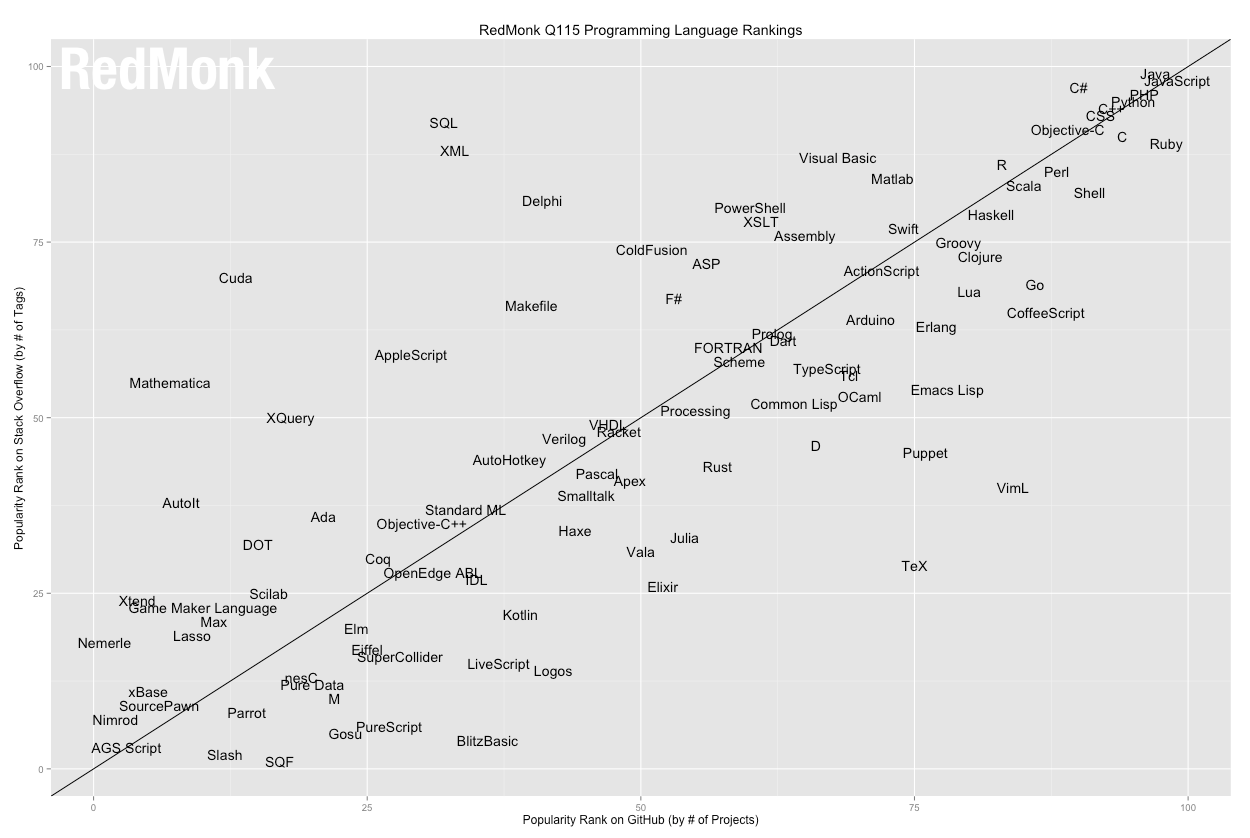
\includegraphics[width=1\textwidth]{img/grafico_redmonk}
	\caption{Ranking das liguagens de programação no Stack Overflow e Github}
\end{figure}


Ainda assim, para compor a interface do dado projeto, também ocorrerá o uso do líder JavaScript de forma intensa, provendo o elo com o as informações gerenciadas pelo PHP.


Entretanto, não seria inteligente desenvolver um sistema completo sem o auxílio de um framework. Dentre os frameworks disponíveis para PHP, hoje o destaque está com o Laravel, que se encontra no topo dentre os mais utilizados no momento. 


A WebHostFace, uma empresa de hospedagem, compilou várias estatísticas para criar um infográfico mostrando os frameworks PHP mais populares de 2015. Utilizando informações sobre os próprios clientes, o Google Trends, estatísticas de repositórios do GitHub e a pesquisa do SitePoint “Best PHP Frameworks 2015”, a WebHostFace elaborou o seguinte infográfico: 

\begin{figure}
	\label{fig:graficoWebhostface}
	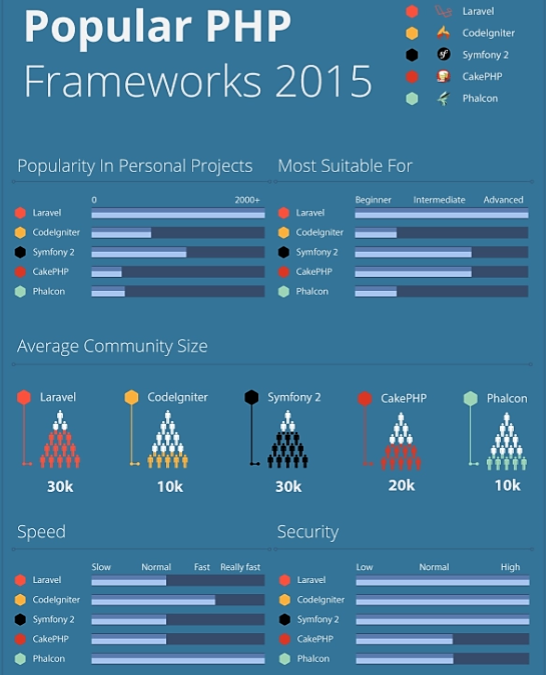
\includegraphics[width=1\textwidth]{img/infografico_webhostface}
	\caption{Infográfico da WebhostFace, exibindo a popularidade dos Frameworks PHP em 2015}
\end{figure}

Assim, tem-se a evidência que o Laravel em 2015 teve a maior popularidade em projetos pessoais e tem a maior comunidade entre os concorrentes, o que o torna uma boa escolha para a escrita de um software que será continuado por terceiros.


Para elaborar os recursos de interface e integrar ao back-end PHP do sistema, será adotado o já conhecido AngularJS, ferramenta sólida e conhecida no aspecto em questão. 


Dados coletados via Google Trends, que propõe comparações entre termos pesquisados, revela a popularidade do AngularJs diante de alguns dos principais concorrentes. O gráfico abaixo evidencia o cenário.


%Como mostra a Figura \ref{fig:graficoGoogleTrendsFerramentasFront}. 
\begin{figure}
	\label{fig:graficoGoogleTrendsFerramentasFront}
	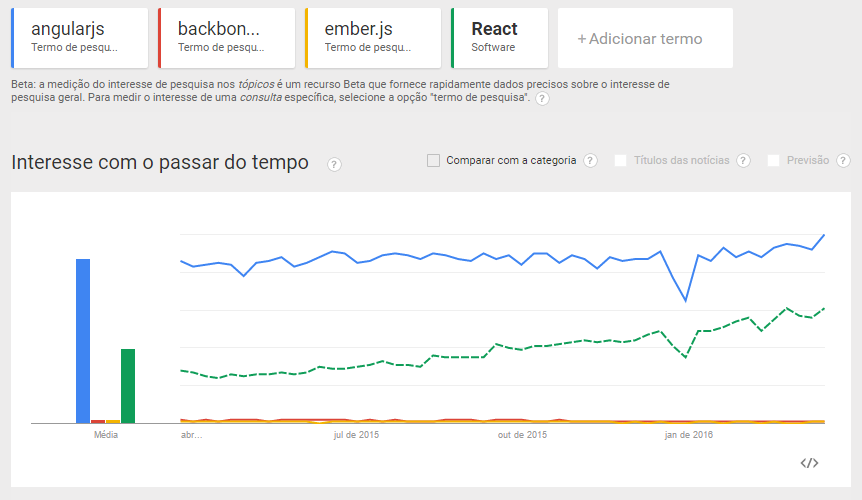
\includegraphics[width=1\textwidth]{img/grafico_ferramentas_front}
	\caption{Gráfico do Google Trends exibindo as pesquisas por ferramentas front-end}
\end{figure}


Junto ao Angular JS, será utilizada a agradável tendência de interface do Material Design da Google, que propõe layouts limpos e otimizados já conhecidos pelos usuários de smartphones Android. 


Para a elaboração da plataforma mobile do projeto, será utilizado o Ionic Framework, muito difundido e bastante pesquisado na área, o que fica evidenciado com o gráfico de pesquisbaixo, coletado via Google Trends buscando por frameworks de desenvolvimento híbrido mobile.


\begin{figure}
	\label{fig:graficoGoogleTrendsFerramentasHibridasMobile}
	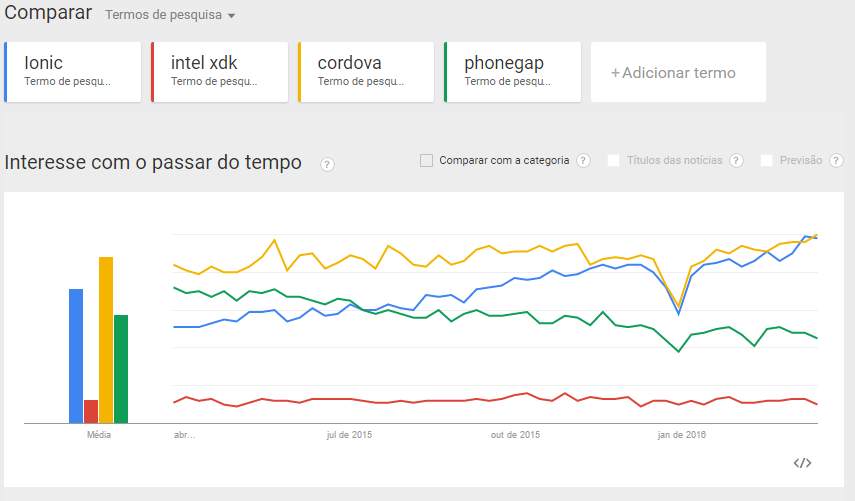
\includegraphics[width=1\textwidth]{img/grafico_ferramentas_hibridas_mobile}
	\caption{Gráfico do Google Trends exibindo as pesquisas por Frameworks híbridos mobile}
\end{figure}	

Para layout da interface mobile, também será aplicado a tendência do Material Design, a fim de propor uma harmonia entre o módulo web e mobile para os usuários


\section{Resultados Esperados}


Como fruto de um sistema para pós-graduação da UFBA, espera-se que os professores tenham mais recursos para integrar as atividades e também prover melhores condições para acompanhamento da vida acadêmica dos alunos em questão. Também, que os novos colaboradores que entrarem no processo tenham facilidade de compreender o fluxo do setor ao navegar pelo sistema proposto.


\section{Fora de Escopo}


Interação com os alunos devido às complicações para realizar a integração com o sistema empregado na UFBA, gerenciado pela XXXXXX, o que causaria uma inviabilidade no projeto devido à necessidade de entrega do produto ser mais forte que o tempo necessário para executar o processo de obtenção de acesso ao sistema legado para realizar a integração.


\section{Estrutura do Trabalho}


<breve resumo sobre os capítulos do TCC>
\chapter{Referencial Teórico}


Projetar o desenvolvimento de um software requer muito planejamento, pois as falhas iniciais podem custar bastante caro ou até mesmo inviabilizar a continuação de um projeto. Assim, a escolha da arquitetura ideal para a aplicabilidade é essencial na concepção de um produto de software. 
De todo o modo, sempre busca-se fazer mais com menos. Diante de tal filosofia, temos nesta seção, uma breve discussão sobre alguns elementos de projeto e arquitetura de software, a fim de contextualizar este trabalho de conclusão de curso.


% Ser direto no começo, focando no que realmente será discutido A seção \ref{sec:apps_mobile} 
 \section{Software como serviço}\label{sec:saas}


A definição de SaaS encontra-se muito bem elaborada em um dos trabalhos listados na literatura. Segundo La e Chun \citep{La2009Systematic}, o princípio da definição de Software como um Serviço (Sofware as a Service - SaaS) é um serviço complementar para aplicações da computação em nuvem (cloud computing). As duas áreas estão interligadas, no entanto, não se confundem, pois o SaaS deve ser entendido como um mecanismo de suporte às soluções existentes na cloud. Os SaaS existem justamente para maximizar o reuso de serviços repetidos e não centrais em uma aplicação remota.


Como propõe vantagens, software como servico é uma tendência forte, isso graças à evolução da web. Diversos fatores podem ser favoráveis para a adoção de um SaaS, como custo e manutenção dentre outros fatores aplicaveis a determinados contextos. Um trabalho recente realizado por Lechessa et al. \cite{LechesaSS11} apresenta uma pesquisa qualitativa sobre os fatores determinantes para adoção ou não de um SaaS voltado para ERP na África do Sul. Esses autores indicam que os principais fatores determinantes para adoção desse mecanismo de software são sua fluidez quanto à rede e a segurança. Esses fatores estão presentes na aplicação desenvolvida neste trabalho de conclusão de curso.
 

Devido ao fato de ter um serviço constantemente na nuvem, fica o questionamento sobre a segurança da informação manipulada. Sabe-se que a vulnerabilidade na web não é restrita ao SaaS, atingindo diversos âmbitos. O artigo de Rai et al. \cite{journals/corr/RaiSM13} orienta como o avanço da computação em nuvem não é um problema apenas para os serviços web do ponto de vista da segurança, pois muitos trabalhos na literatura mostram a área como mais um ponto de vulnerabilidade para diversos setores, a exemplo de infraestrutura. No mesmo artigo mencionado de Rai et al. \cite{journals/corr/RaiSM13}, também realizaram-se estudos exploratórios junto a empresas usuárias de serviços em computação em nuvem e consideram que a perspectiva de SaaS também pode fortalecer a segurança nas aplicações de cloud computing, pois o software de autenticação compartilhado por várias aplicações em nuvem, oferece uma melhor padronização e consequente facilidade de prevenção a erros de vulnerabilidade específicas de cada módulo da pesquisa. Esse ponto de vista é muito importante para qualquer trabalho de ponta na área de SaaS.


A arquitetura de armazenamento de dados de um Saas pode variar de acordo com a necessidade do contexto. O artigo recente de Huixin \cite{7586486}, exemplifica possíveis modelagens para utilizar. Tal abordagem pode ser com um banco de dados único, fazendo com que diferentes clientes compartilhem o mesmo banco, diferindo os dados através de controle de usuário, ou isolando os diferentes clientes através de bancos de dados exclusivos para cada um. Tal fator também pode ser combinado com a arquitetura da aplicação, caso ofereça aplicação única para todos os clientes ou aplicação compartilhada. Diante das possíveis abprdagens, a modelagem de dados do software pode ser decidida pela regra de negócio. Este trabalho optou por aplicação única e banco de dados compartilhado.


Devido ao diferente conceito de obtenção de software, tanto pela visão do cliente como pela visão do vendedor, é necessário tomar conhecimento dos diversos fatores que podem ser relevantes ao orçar um Saas. O recente trabalho de T. Kaur et al. \citep{6949281} orienta um modelo para compor o custo de um Saas. O custo total seria composto pelos fatores que dão suporte ao funcionamento do software. Tais fatores incluem infra-estrutura, configurabilidade, customização, parâmetros de QoS(Quality of service) como escalabilidade, disponibilidade, usabilidade, pontualidade e desempenho da resposta, portabilidade, custo total de propriedade e retorno do investimento. Esses fatores caracterizam o custo de forma eficaz, possibilitando ao fornecedor, prover um Serviço de acordo com a exigência do consumidor em vários pacotes de serviços.


\section{Reuso de software}\label{sec:reuso} %CRUISE BOOK CAPITULO 2


Para Peter Freeman, o reuso é a utilização de qualquer informação que um desenvolvedor pode necessitar no processo de criação de software (Ezran et al., 2002). Basili e Rombach definem reutilização de software como o uso de tudo o que está associado a um projeto de conhecimento (Basili e Rombach, 1991).
Assim, o objetivo da reutilização de software é reciclar o design, código e outros componentes de um produto de software e assim reduzir o custo, o tempo e melhorar a qualidade do produto.
Segundo Keswani et al. \cite{6783445}, o componente reutilizável de software pode ser qualquer parte de seu desenvolvimento, como um fragmento de código, design, casos de teste, ou até mesmo a especificação de requisitos de uma funcionalidade do software. 

O reuso de software pode ter impacto positivo em diversos aspectos do software, vejamos alguns, conforme apresentados no C.R.U.I.S.E Book:

\begin{itemize}

\item Qualidade: As correções de erro tornam-se úteis em todos os locais em que ocorreu, padronizando e facilitando a manutenção.

\item Produtividade: O ganho de produtividade é alcançado devido ao menor número de artefatos desenvolvido. Isso resulta em menos esforços de teste e também economiza análise e design, gerando economia em diversos escopos do projeto.

\item Confiabilidade: A utilização de componentes bem testados aumenta a
confiança no software. Além disso, a utilização de um mesmo componente em vários sistemas, aumenta a possibilidade de detecção de erros e reforça a confiança no componente.

\item Redução do Esforço: A reutilização de software proporciona uma redução do tempo de desenvolvimento, o que reduz o tempo necessário para o produto ser disponibilizado no mercado para trazer rentabilidade.

\item Trabalho redundante e tempo de desenvolvimento: Desenvolver um sistema do
zero significa desenvolvimento redundante de muitos componentes, como requisito
especificações, casos de uso, arquitetura, etc. Isso pode ser evitado quando estes estão disponíveis como componentes reutilizáveis e podem ser compartilhados, resultando em menos desenvolvimento, tempo e custo associado.

\item Documentação: Embora a documentação seja muito importante para a
manutenção de um sistema, muitas vezes é negligenciada. A reutilização de componentes software reduz a quantidade de documentação a ser escrita, entretanto depende da qualidade do que está escrito. Assim, apenas a estrutura do sistema e os novos artefatos desenvolvidos necessitam ser documentados.

\item Custo de manutenção: Menos defeitos e manutenções são esperados quando tem-se comprovada a qualidade dos componentes utilizados.

\item Tamanho da equipe: É comum entrar casos em que a equipe de desenvolvimento sofre sobrecarga. Entretanto, dobrar o tamanho da equipe de desenvolvimento não necessariamente duplica produtividade. Se muitos componentes podem ser reutilizados, é possível desenvolver com equipes menores, levando a melhores comunicações e aumento da produtividade.

\end{itemize}

Apesar dos benefícios da reutilização de software, a mesma não é amplamente praticado como imagina-se. Existem fatores que influenciam direta ou indiretamente na sua adoção. Esses fatores podem ser de aspecto gerencial, organizacional, econômico, conceitual ou técnico. Veremos a seguir alguns aspectos que podem gerar conflito com a cultura de reuso de software, segundo o C.R.U.I.S.E Book:
%(Sametinger, 1997). REVER

\begin{itemize}
	
\item Falta de apoio da gestão: Como a reutilização de software gera custos iniciais,
a medida pode não ser amplamente alcançada em uma organização sem o apoio de alto nível gestão. Os gestores têm de ser informados sobre os custos iniciais e serem convencidos sobre economias futuras.

\item Gerenciamento do Projeto: Gerenciar projetos tradicionais é uma tarefa árdua, principalmente, os que praticam a reutilização de software. Utilizando a técnica em larga escala, tem-se impacto sobre todo o ciclo de vida do software.

\item Estruturas organizacionais inadequadas: As estruturas organizacionais devem
considerar diferentes necessidades que surgem quando a reutilização em larga escala está sendo adotada. Por exemplo, uma equipe particionada pode ser alocada somente para desenvolver, manter e certificar componentes reutilizáveis de software.

\item Incentivos de gestão: É comum a falta de incentivo para deixar os desenvolvedores gastarem tempo elaborando reutilizáveis componentes do sistema. A produtividade é muitas vezes medida apenas no tempo necessário para concluir um projeto. Assim, fazer qualquer trabalho além disso, embora benéfico para a empresa como um todo, diminui o seu sucesso. Mesmo quando os componentes reutilizáveis são utilizados, os benefícios obtidos são uma pequena fração do que poderia ser alcançado caso houvesse reutilização explícita, planejada e organizada.

\item Dificuldade de encontrar software reutilizável: Para reutilizar os componentes, devem existir formas eficientes de busca. Além disso, é importante ter um repositório bem organizado contendo componentes com um eficiente meio de acesso.

\item Não reutilização do software encontrado. O acesso fácil ao software existente
não necessariamente aumentar a reutilização. Os componentes reutilizáveis devem ser cuidadosamente especificados, projetados, implementados e documentados, pois em alguns casos, modificar e adaptar o código  pode ser mais custoso que a programação da funcionalidade necessária a partir do zero.

\item Modificação: É muito difícil encontrar um componente que funcione
exatamente da mesma maneira que queremos. Desta forma, são necessárias modificações e devem existir formas de determinar os seus efeitos sobre o componente.


\end{itemize}


%Outra diretriz importante para a reutilização de software é reduzir o risco na criação de novos softwares. O risco tende a ser bastante reduzido se os componentes que estão sendo reutilizados têm as documentação, interfaces necessárias e devidamente testadas, fatores que contibruem para uma fácil integração.
%De acordo com Keswani et al. \citep{6783445}, para o reuso de software dar retornos apropriados, o processo deve ser sistemático e planejado. Qualquer organização que implemente a reutilização de software deve identificar os melhores métodos e estratégias de reutilização para obter a máxima produtividade. A reutilização de software ajuda a evitar software de engenharia a partir do zero, pois usa módulos de software existentes. A reutilização de software, embora seja uma tarefa difícil, especialmente para softwares antigos sem padrões de projeto, pode melhorar significativamente a produtividade e a qualidade de um produto de software. Embora a reutilização de software não seja um novo campo, ela pode dar grandes retornos em curto período de tempo.


\section{Modularização}\label{sec:modularizacao} %artigo de claudio pagina 222 introdução


%A modularidade vem desempenhando um papel predominante estágios emergentes das disciplinas de arquitetura de software [13]. Engenheiros de software consideram modularidade como princípio base na comparação entre arquiteturas alternativas  e arquitetura degeneração [9]. De fato, os engenheiros de software são incentivados a arquitecturas, baseando-se numa multiplicidade de mecanismos de modularidade disponíveis em: 
%(i) Linguagens de descrição de arquitetura (ADLs), como ACME [8], 
%(ii) catálogos de arquitetônicos [2, 13], e 
%(iii) conhecem bem princípios de alto nível, como interfaces de componentes estreitos, acoplamento arquitectónico reduzido e semelhantes.


Conforme é frisado no trabalho de Wickramaarachchi e Lai \citep{7062705}, o conceito de modularização na indústria de software tem uma longa história e tem sido utilizado para melhorar o processo de desenvolvimento de software em diferentes estágios. Os principais conceitos por trás da modularização do software foram introduzidos por pesquisadores pioneiros há quarenta anos, com uma notável contribuição feita por Melvin Conway e David Parnas, que tem representação notável na engenharia de software.


Modularizar um software é um bom padrão a ser adotado. Segundo Wickramaarachchi e Lai \citep{7062705}, a modularização é importante na identificação de dependências e reduz as dificuldades diante de uma possível necessidade de grandes alterações. De uma perspectiva da engenharia de software, uma modularização geralmente tem várias vantagens, tais como: tornar a complexidade do software mais gerenciável, facilitar o trabalho paralelo e tornar o software mais maleável para acomodar o futuro incerto que um software pode ter. O objetivo final da modularização do software é aumentar a produtividade ea qualidade do software. Tal conceito encontra-se bastante difundido e estái incorporado em linguagens de programação e ferramentas de software. O trabalho proposto favorece ao uso da modularização de um software e até mesmo pode ser considerado um módulo a ser acoplado a qualquer software, mediante a compatibilidade.


\section{Aplicações web}\label{sec:apps_web}


A popularidade da aplicação web aumentou exponencialmente na última década e todos os dias cresce o número de pessoas usuárias de aplicações web. E seguindo o padrão de desenvolvimento de software, Kumar et al. \citep{7813710} sugerem que para o desenvolvimento web, deve-se manter a prática efiacaz de produzir diagramas UML. A abordagem baseada na web oferece uma maneira fácil e eficaz para gerenciar e controlar o processo de desenvolvimento por meio de diagramas UML. Tal abordagem pode ser usada quando há uma exigência de lidar com mudanças muito rápidas e grandes em requisitos de forma muito eficaz em muito menos tempo, gerando assim um menor impacto. 


Para atender à fomentada demanda de aplicativos web, é necessário adotar métodos de desenvolvimentos que sejam ágeis, eficientes e de fácil manutenção. Yu Ping et al. \cite{1372143} propõem o uso do modelo MVC (Model, View e Controller) no atual desenvolvimento para softwares web. O modelo apresentado tornou-se um padrão popular e divide o software em camadas com propósito definido, tornando-o de mais fácil manutenção.


O Ajax (Asynchronous Javascript and XML) revolucionou a web. Conforme demonstrado no artigo de Yuping \citep{6845605}, ao usar a tecnologia Ajax, podemos enriquecer a experiência do usuário em aplicações baseadas em navegador de internet, e fornecer uma variedade de aplicações interativas para atender às necessidade de humanização das aplicações.
Os aplicativos Ajax em execução no navegador se comunicam com um servidor Web de forma assíncrona e atualizam apenas uma parte da página.



% %% RiSE Latex Template - version 0.5
%%
%% RiSE's latex template for thesis and dissertations
%% http://risetemplate.sourceforge.net
%%
%% (c) 2012 Yguaratã Cerqueira Cavalcanti (yguarata@gmail.com)
%%          Vinicius Cardoso Garcia (vinicius.garcia@gmail.com)
%%
%% This document was initially based on UFPEThesis template, from Paulo Gustavo
%% S. Fonseca.
%%
%% ACKNOWLEDGEMENTS
%%
%% We would like to thanks the RiSE's researchers community, the 
%% students from Federal University of Pernambuco, and other users that have
%% been contributing to this projects with comments and patches.
%%
%% GENERAL INSTRUCTIONS
%%
%% We strongly recommend you to compile your documents using pdflatex command.
%% It is also recommend use the texlipse plugin for Eclipse to edit your documents.
%%
%% Options for \documentclass command:
%%         * Idiom
%%           pt   - Portguese (default)
%%           en   - English
%%
%%         * Text type
%%           bsc  - B.Sc. Thesis
%%           msc  - M.Sc. Thesis (default)
%%           qual - PHD qualification (not tested yet)
%%           prop - PHD proposal (not tested yet)
%%           phd  - PHD thesis
%%
%%         * Media
%%           scr  - to eletronic version (PDF) / see the users guide
%%
%%         * Pagination
%%           oneside - unique face press
%%           twoside - two faces press
%%
%%		   * Line spacing
%%           singlespacing  - the same as using \linespread{1}
%%           onehalfspacing - the same as using \linespread{1.3}
%%           doublespacing  - the same as using \linespread{1.6}
%%
%% Reference commands. Use the following commands to make references in your
%% text:
%%          \figref  -- for Figure reference
%%          \tabref  -- for Table reference
%%          \eqnref  -- for equation reference
%%          \chapref -- for chapter reference
%%          \secref  -- for section reference
%%          \appref  -- for appendix reference
%%          \axiref  -- for axiom reference
%%          \conjref -- for conjecture reference
%%          \defref  -- for definition reference
%%          \lemref  -- for lemma reference
%%          \theoref -- for theorem reference
%%          \corref  -- for corollary reference
%%          \propref -- for proprosition reference
%%          \pgref   -- for page reference
%%
%%          Example: See \chapref{chap:introduction}. It will produce 
%%                   'See Chapter 1', in case of English language.

\documentclass[pt,twoside,onehalfspacing,bsc]{risethesis}

\usepackage[utf8]{inputenc}
\usepackage[brazilian]{babel}
\usepackage[T1]{fontenc}

%% Change the following pdf author attribute name to your name.
\usepackage[linkcolor=blue,citecolor=blue,urlcolor=blue,colorlinks,pdfpagelabels,pdftitle={Bruno Cabral's Bachelor Thesis},pdfauthor={Bruno Cabral}]{hyperref}

\address{SALVADOR}

\universitypt{Universidade Federal da Bahia}
\universityen{Federal University of Bahia}

\departmentpt{Depertamento de Ciência da Computação}
\departmenten{Computer Science Department}

\programpt{Programa Multiinstitucional de Pós-graduação em Ciência da Computação}
\programen{Graduate in Computer Science}

\majorfieldpt{Ciência da Computação}
\majorfielden{Computer Science}

\title{Sistema de apoio à Pós graduação - UFBA}
\date{Outubro/2016}

\author{Victor de Azevedo Nunes}
\adviser{Ivan do Carmo Machado}

\begin{document}

\frontmatter
\frontpage
\presentationpage

\begin{dedicatory}
Eu dedico esta dissertação...
%I dedicate this dissertation to my family, girlfriend, friends and
%professors who gave me all necessary support to get here.
\end{dedicatory}

\acknowledgements
Meus agradecimentos...

\begin{epigraph}[]{Edward V Berard}
Walking on water and developing software from a specification are easy if both are frozen
\end{epigraph}

\resumo
% Escreva seu resumo no arquivo resumo.tex
\input{resumo}

\abstract
% Write your abstract in a file called abstract.tex
\input{abstract}

% Summary (tables of contents)
\tableofcontents

% List of figures
\listoffigures

% List of tables
\listoftables

% List of acronyms
% Acronyms manual: http://linorg.usp.br/CTAN/macros/latex/contrib/acronym/acronym.pdf
\listofacronyms
\input{acronyms}

% List of listings
%\lstlistoflistings

\mainmatter

\include{chapters/intro}
\include{chapters/referencial_teorico}

% \include{chapters/introduction/main}
% \include{chapters/background/main}
% \include{chapters/proposed_solution/main}
% \include{chapters/experiment/main}
% \include{chapters/conclusion/main}

\bibliographystyle{natbib}
\addcontentsline{toc}{chapter}{\bibliographytocname}
\bibliography{references}

% Appendix
\clearpage
\addappheadtotoc
\appendix
\appendixpage
% \include{appendix/experiment-instruments}

\end{document}
% %% RiSE Latex Template - version 0.5
%%
%% RiSE's latex template for thesis and dissertations
%% http://risetemplate.sourceforge.net
%%
%% (c) 2012 Yguaratã Cerqueira Cavalcanti (yguarata@gmail.com)
%%          Vinicius Cardoso Garcia (vinicius.garcia@gmail.com)
%%
%% This document was initially based on UFPEThesis template, from Paulo Gustavo
%% S. Fonseca.
%%
%% ACKNOWLEDGEMENTS
%%
%% We would like to thanks the RiSE's researchers community, the 
%% students from Federal University of Pernambuco, and other users that have
%% been contributing to this projects with comments and patches.
%%
%% GENERAL INSTRUCTIONS
%%
%% We strongly recommend you to compile your documents using pdflatex command.
%% It is also recommend use the texlipse plugin for Eclipse to edit your documents.
%%
%% Options for \documentclass command:
%%         * Idiom
%%           pt   - Portguese (default)
%%           en   - English
%%
%%         * Text type
%%           bsc  - B.Sc. Thesis
%%           msc  - M.Sc. Thesis (default)
%%           qual - PHD qualification (not tested yet)
%%           prop - PHD proposal (not tested yet)
%%           phd  - PHD thesis
%%
%%         * Media
%%           scr  - to eletronic version (PDF) / see the users guide
%%
%%         * Pagination
%%           oneside - unique face press
%%           twoside - two faces press
%%
%%		   * Line spacing
%%           singlespacing  - the same as using \linespread{1}
%%           onehalfspacing - the same as using \linespread{1.3}
%%           doublespacing  - the same as using \linespread{1.6}
%%
%% Reference commands. Use the following commands to make references in your
%% text:
%%          \figref  -- for Figure reference
%%          \tabref  -- for Table reference
%%          \eqnref  -- for equation reference
%%          \chapref -- for chapter reference
%%          \secref  -- for section reference
%%          \appref  -- for appendix reference
%%          \axiref  -- for axiom reference
%%          \conjref -- for conjecture reference
%%          \defref  -- for definition reference
%%          \lemref  -- for lemma reference
%%          \theoref -- for theorem reference
%%          \corref  -- for corollary reference
%%          \propref -- for proprosition reference
%%          \pgref   -- for page reference
%%
%%          Example: See \chapref{chap:introduction}. It will produce 
%%                   'See Chapter 1', in case of English language.

\documentclass[pt,twoside,onehalfspacing,bsc]{risethesis}

\usepackage[utf8]{inputenc}
\usepackage[brazilian]{babel}
\usepackage[T1]{fontenc}

%% Change the following pdf author attribute name to your name.
\usepackage[linkcolor=blue,citecolor=blue,urlcolor=blue,colorlinks,pdfpagelabels,pdftitle={Bruno Cabral's Bachelor Thesis},pdfauthor={Bruno Cabral}]{hyperref}

\address{SALVADOR}

\universitypt{Universidade Federal da Bahia}
\universityen{Federal University of Bahia}

\departmentpt{Depertamento de Ciência da Computação}
\departmenten{Computer Science Department}

\programpt{Programa Multiinstitucional de Pós-graduação em Ciência da Computação}
\programen{Graduate in Computer Science}

\majorfieldpt{Ciência da Computação}
\majorfielden{Computer Science}

\title{Sistema de apoio à Pós graduação - UFBA}
\date{Outubro/2016}

\author{Victor de Azevedo Nunes}
\adviser{Ivan do Carmo Machado}

\begin{document}

\frontmatter
\frontpage
\presentationpage

\begin{dedicatory}
Eu dedico esta dissertação...
%I dedicate this dissertation to my family, girlfriend, friends and
%professors who gave me all necessary support to get here.
\end{dedicatory}

\acknowledgements
Meus agradecimentos...

\begin{epigraph}[]{Edward V Berard}
Walking on water and developing software from a specification are easy if both are frozen
\end{epigraph}

\resumo
% Escreva seu resumo no arquivo resumo.tex
\input{resumo}

\abstract
% Write your abstract in a file called abstract.tex
\input{abstract}

% Summary (tables of contents)
\tableofcontents

% List of figures
\listoffigures

% List of tables
\listoftables

% List of acronyms
% Acronyms manual: http://linorg.usp.br/CTAN/macros/latex/contrib/acronym/acronym.pdf
\listofacronyms
\input{acronyms}

% List of listings
%\lstlistoflistings

\mainmatter

\include{chapters/intro}
\include{chapters/referencial_teorico}

% \include{chapters/introduction/main}
% \include{chapters/background/main}
% \include{chapters/proposed_solution/main}
% \include{chapters/experiment/main}
% \include{chapters/conclusion/main}

\bibliographystyle{natbib}
\addcontentsline{toc}{chapter}{\bibliographytocname}
\bibliography{references}

% Appendix
\clearpage
\addappheadtotoc
\appendix
\appendixpage
% \include{appendix/experiment-instruments}

\end{document}
% %% RiSE Latex Template - version 0.5
%%
%% RiSE's latex template for thesis and dissertations
%% http://risetemplate.sourceforge.net
%%
%% (c) 2012 Yguaratã Cerqueira Cavalcanti (yguarata@gmail.com)
%%          Vinicius Cardoso Garcia (vinicius.garcia@gmail.com)
%%
%% This document was initially based on UFPEThesis template, from Paulo Gustavo
%% S. Fonseca.
%%
%% ACKNOWLEDGEMENTS
%%
%% We would like to thanks the RiSE's researchers community, the 
%% students from Federal University of Pernambuco, and other users that have
%% been contributing to this projects with comments and patches.
%%
%% GENERAL INSTRUCTIONS
%%
%% We strongly recommend you to compile your documents using pdflatex command.
%% It is also recommend use the texlipse plugin for Eclipse to edit your documents.
%%
%% Options for \documentclass command:
%%         * Idiom
%%           pt   - Portguese (default)
%%           en   - English
%%
%%         * Text type
%%           bsc  - B.Sc. Thesis
%%           msc  - M.Sc. Thesis (default)
%%           qual - PHD qualification (not tested yet)
%%           prop - PHD proposal (not tested yet)
%%           phd  - PHD thesis
%%
%%         * Media
%%           scr  - to eletronic version (PDF) / see the users guide
%%
%%         * Pagination
%%           oneside - unique face press
%%           twoside - two faces press
%%
%%		   * Line spacing
%%           singlespacing  - the same as using \linespread{1}
%%           onehalfspacing - the same as using \linespread{1.3}
%%           doublespacing  - the same as using \linespread{1.6}
%%
%% Reference commands. Use the following commands to make references in your
%% text:
%%          \figref  -- for Figure reference
%%          \tabref  -- for Table reference
%%          \eqnref  -- for equation reference
%%          \chapref -- for chapter reference
%%          \secref  -- for section reference
%%          \appref  -- for appendix reference
%%          \axiref  -- for axiom reference
%%          \conjref -- for conjecture reference
%%          \defref  -- for definition reference
%%          \lemref  -- for lemma reference
%%          \theoref -- for theorem reference
%%          \corref  -- for corollary reference
%%          \propref -- for proprosition reference
%%          \pgref   -- for page reference
%%
%%          Example: See \chapref{chap:introduction}. It will produce 
%%                   'See Chapter 1', in case of English language.

\documentclass[pt,twoside,onehalfspacing,bsc]{risethesis}

\usepackage[utf8]{inputenc}
\usepackage[brazilian]{babel}
\usepackage[T1]{fontenc}

%% Change the following pdf author attribute name to your name.
\usepackage[linkcolor=blue,citecolor=blue,urlcolor=blue,colorlinks,pdfpagelabels,pdftitle={Bruno Cabral's Bachelor Thesis},pdfauthor={Bruno Cabral}]{hyperref}

\address{SALVADOR}

\universitypt{Universidade Federal da Bahia}
\universityen{Federal University of Bahia}

\departmentpt{Depertamento de Ciência da Computação}
\departmenten{Computer Science Department}

\programpt{Programa Multiinstitucional de Pós-graduação em Ciência da Computação}
\programen{Graduate in Computer Science}

\majorfieldpt{Ciência da Computação}
\majorfielden{Computer Science}

\title{Sistema de apoio à Pós graduação - UFBA}
\date{Outubro/2016}

\author{Victor de Azevedo Nunes}
\adviser{Ivan do Carmo Machado}

\begin{document}

\frontmatter
\frontpage
\presentationpage

\begin{dedicatory}
Eu dedico esta dissertação...
%I dedicate this dissertation to my family, girlfriend, friends and
%professors who gave me all necessary support to get here.
\end{dedicatory}

\acknowledgements
Meus agradecimentos...

\begin{epigraph}[]{Edward V Berard}
Walking on water and developing software from a specification are easy if both are frozen
\end{epigraph}

\resumo
% Escreva seu resumo no arquivo resumo.tex
\input{resumo}

\abstract
% Write your abstract in a file called abstract.tex
\input{abstract}

% Summary (tables of contents)
\tableofcontents

% List of figures
\listoffigures

% List of tables
\listoftables

% List of acronyms
% Acronyms manual: http://linorg.usp.br/CTAN/macros/latex/contrib/acronym/acronym.pdf
\listofacronyms
\input{acronyms}

% List of listings
%\lstlistoflistings

\mainmatter

\include{chapters/intro}
\include{chapters/referencial_teorico}

% \include{chapters/introduction/main}
% \include{chapters/background/main}
% \include{chapters/proposed_solution/main}
% \include{chapters/experiment/main}
% \include{chapters/conclusion/main}

\bibliographystyle{natbib}
\addcontentsline{toc}{chapter}{\bibliographytocname}
\bibliography{references}

% Appendix
\clearpage
\addappheadtotoc
\appendix
\appendixpage
% \include{appendix/experiment-instruments}

\end{document}
% %% RiSE Latex Template - version 0.5
%%
%% RiSE's latex template for thesis and dissertations
%% http://risetemplate.sourceforge.net
%%
%% (c) 2012 Yguaratã Cerqueira Cavalcanti (yguarata@gmail.com)
%%          Vinicius Cardoso Garcia (vinicius.garcia@gmail.com)
%%
%% This document was initially based on UFPEThesis template, from Paulo Gustavo
%% S. Fonseca.
%%
%% ACKNOWLEDGEMENTS
%%
%% We would like to thanks the RiSE's researchers community, the 
%% students from Federal University of Pernambuco, and other users that have
%% been contributing to this projects with comments and patches.
%%
%% GENERAL INSTRUCTIONS
%%
%% We strongly recommend you to compile your documents using pdflatex command.
%% It is also recommend use the texlipse plugin for Eclipse to edit your documents.
%%
%% Options for \documentclass command:
%%         * Idiom
%%           pt   - Portguese (default)
%%           en   - English
%%
%%         * Text type
%%           bsc  - B.Sc. Thesis
%%           msc  - M.Sc. Thesis (default)
%%           qual - PHD qualification (not tested yet)
%%           prop - PHD proposal (not tested yet)
%%           phd  - PHD thesis
%%
%%         * Media
%%           scr  - to eletronic version (PDF) / see the users guide
%%
%%         * Pagination
%%           oneside - unique face press
%%           twoside - two faces press
%%
%%		   * Line spacing
%%           singlespacing  - the same as using \linespread{1}
%%           onehalfspacing - the same as using \linespread{1.3}
%%           doublespacing  - the same as using \linespread{1.6}
%%
%% Reference commands. Use the following commands to make references in your
%% text:
%%          \figref  -- for Figure reference
%%          \tabref  -- for Table reference
%%          \eqnref  -- for equation reference
%%          \chapref -- for chapter reference
%%          \secref  -- for section reference
%%          \appref  -- for appendix reference
%%          \axiref  -- for axiom reference
%%          \conjref -- for conjecture reference
%%          \defref  -- for definition reference
%%          \lemref  -- for lemma reference
%%          \theoref -- for theorem reference
%%          \corref  -- for corollary reference
%%          \propref -- for proprosition reference
%%          \pgref   -- for page reference
%%
%%          Example: See \chapref{chap:introduction}. It will produce 
%%                   'See Chapter 1', in case of English language.

\documentclass[pt,twoside,onehalfspacing,bsc]{risethesis}

\usepackage[utf8]{inputenc}
\usepackage[brazilian]{babel}
\usepackage[T1]{fontenc}

%% Change the following pdf author attribute name to your name.
\usepackage[linkcolor=blue,citecolor=blue,urlcolor=blue,colorlinks,pdfpagelabels,pdftitle={Bruno Cabral's Bachelor Thesis},pdfauthor={Bruno Cabral}]{hyperref}

\address{SALVADOR}

\universitypt{Universidade Federal da Bahia}
\universityen{Federal University of Bahia}

\departmentpt{Depertamento de Ciência da Computação}
\departmenten{Computer Science Department}

\programpt{Programa Multiinstitucional de Pós-graduação em Ciência da Computação}
\programen{Graduate in Computer Science}

\majorfieldpt{Ciência da Computação}
\majorfielden{Computer Science}

\title{Sistema de apoio à Pós graduação - UFBA}
\date{Outubro/2016}

\author{Victor de Azevedo Nunes}
\adviser{Ivan do Carmo Machado}

\begin{document}

\frontmatter
\frontpage
\presentationpage

\begin{dedicatory}
Eu dedico esta dissertação...
%I dedicate this dissertation to my family, girlfriend, friends and
%professors who gave me all necessary support to get here.
\end{dedicatory}

\acknowledgements
Meus agradecimentos...

\begin{epigraph}[]{Edward V Berard}
Walking on water and developing software from a specification are easy if both are frozen
\end{epigraph}

\resumo
% Escreva seu resumo no arquivo resumo.tex
\input{resumo}

\abstract
% Write your abstract in a file called abstract.tex
\input{abstract}

% Summary (tables of contents)
\tableofcontents

% List of figures
\listoffigures

% List of tables
\listoftables

% List of acronyms
% Acronyms manual: http://linorg.usp.br/CTAN/macros/latex/contrib/acronym/acronym.pdf
\listofacronyms
\input{acronyms}

% List of listings
%\lstlistoflistings

\mainmatter

\include{chapters/intro}
\include{chapters/referencial_teorico}

% \include{chapters/introduction/main}
% \include{chapters/background/main}
% \include{chapters/proposed_solution/main}
% \include{chapters/experiment/main}
% \include{chapters/conclusion/main}

\bibliographystyle{natbib}
\addcontentsline{toc}{chapter}{\bibliographytocname}
\bibliography{references}

% Appendix
\clearpage
\addappheadtotoc
\appendix
\appendixpage
% \include{appendix/experiment-instruments}

\end{document}
% %% RiSE Latex Template - version 0.5
%%
%% RiSE's latex template for thesis and dissertations
%% http://risetemplate.sourceforge.net
%%
%% (c) 2012 Yguaratã Cerqueira Cavalcanti (yguarata@gmail.com)
%%          Vinicius Cardoso Garcia (vinicius.garcia@gmail.com)
%%
%% This document was initially based on UFPEThesis template, from Paulo Gustavo
%% S. Fonseca.
%%
%% ACKNOWLEDGEMENTS
%%
%% We would like to thanks the RiSE's researchers community, the 
%% students from Federal University of Pernambuco, and other users that have
%% been contributing to this projects with comments and patches.
%%
%% GENERAL INSTRUCTIONS
%%
%% We strongly recommend you to compile your documents using pdflatex command.
%% It is also recommend use the texlipse plugin for Eclipse to edit your documents.
%%
%% Options for \documentclass command:
%%         * Idiom
%%           pt   - Portguese (default)
%%           en   - English
%%
%%         * Text type
%%           bsc  - B.Sc. Thesis
%%           msc  - M.Sc. Thesis (default)
%%           qual - PHD qualification (not tested yet)
%%           prop - PHD proposal (not tested yet)
%%           phd  - PHD thesis
%%
%%         * Media
%%           scr  - to eletronic version (PDF) / see the users guide
%%
%%         * Pagination
%%           oneside - unique face press
%%           twoside - two faces press
%%
%%		   * Line spacing
%%           singlespacing  - the same as using \linespread{1}
%%           onehalfspacing - the same as using \linespread{1.3}
%%           doublespacing  - the same as using \linespread{1.6}
%%
%% Reference commands. Use the following commands to make references in your
%% text:
%%          \figref  -- for Figure reference
%%          \tabref  -- for Table reference
%%          \eqnref  -- for equation reference
%%          \chapref -- for chapter reference
%%          \secref  -- for section reference
%%          \appref  -- for appendix reference
%%          \axiref  -- for axiom reference
%%          \conjref -- for conjecture reference
%%          \defref  -- for definition reference
%%          \lemref  -- for lemma reference
%%          \theoref -- for theorem reference
%%          \corref  -- for corollary reference
%%          \propref -- for proprosition reference
%%          \pgref   -- for page reference
%%
%%          Example: See \chapref{chap:introduction}. It will produce 
%%                   'See Chapter 1', in case of English language.

\documentclass[pt,twoside,onehalfspacing,bsc]{risethesis}

\usepackage[utf8]{inputenc}
\usepackage[brazilian]{babel}
\usepackage[T1]{fontenc}

%% Change the following pdf author attribute name to your name.
\usepackage[linkcolor=blue,citecolor=blue,urlcolor=blue,colorlinks,pdfpagelabels,pdftitle={Bruno Cabral's Bachelor Thesis},pdfauthor={Bruno Cabral}]{hyperref}

\address{SALVADOR}

\universitypt{Universidade Federal da Bahia}
\universityen{Federal University of Bahia}

\departmentpt{Depertamento de Ciência da Computação}
\departmenten{Computer Science Department}

\programpt{Programa Multiinstitucional de Pós-graduação em Ciência da Computação}
\programen{Graduate in Computer Science}

\majorfieldpt{Ciência da Computação}
\majorfielden{Computer Science}

\title{Sistema de apoio à Pós graduação - UFBA}
\date{Outubro/2016}

\author{Victor de Azevedo Nunes}
\adviser{Ivan do Carmo Machado}

\begin{document}

\frontmatter
\frontpage
\presentationpage

\begin{dedicatory}
Eu dedico esta dissertação...
%I dedicate this dissertation to my family, girlfriend, friends and
%professors who gave me all necessary support to get here.
\end{dedicatory}

\acknowledgements
Meus agradecimentos...

\begin{epigraph}[]{Edward V Berard}
Walking on water and developing software from a specification are easy if both are frozen
\end{epigraph}

\resumo
% Escreva seu resumo no arquivo resumo.tex
\input{resumo}

\abstract
% Write your abstract in a file called abstract.tex
\input{abstract}

% Summary (tables of contents)
\tableofcontents

% List of figures
\listoffigures

% List of tables
\listoftables

% List of acronyms
% Acronyms manual: http://linorg.usp.br/CTAN/macros/latex/contrib/acronym/acronym.pdf
\listofacronyms
\input{acronyms}

% List of listings
%\lstlistoflistings

\mainmatter

\include{chapters/intro}
\include{chapters/referencial_teorico}

% \include{chapters/introduction/main}
% \include{chapters/background/main}
% \include{chapters/proposed_solution/main}
% \include{chapters/experiment/main}
% \include{chapters/conclusion/main}

\bibliographystyle{natbib}
\addcontentsline{toc}{chapter}{\bibliographytocname}
\bibliography{references}

% Appendix
\clearpage
\addappheadtotoc
\appendix
\appendixpage
% \include{appendix/experiment-instruments}

\end{document}

\bibliographystyle{natbib}
\addcontentsline{toc}{chapter}{\bibliographytocname}
\bibliography{references}

% Appendix
\clearpage
\addappheadtotoc
\appendix
\appendixpage
% \include{appendix/experiment-instruments}

\end{document}
% %% RiSE Latex Template - version 0.5
%%
%% RiSE's latex template for thesis and dissertations
%% http://risetemplate.sourceforge.net
%%
%% (c) 2012 Yguaratã Cerqueira Cavalcanti (yguarata@gmail.com)
%%          Vinicius Cardoso Garcia (vinicius.garcia@gmail.com)
%%
%% This document was initially based on UFPEThesis template, from Paulo Gustavo
%% S. Fonseca.
%%
%% ACKNOWLEDGEMENTS
%%
%% We would like to thanks the RiSE's researchers community, the 
%% students from Federal University of Pernambuco, and other users that have
%% been contributing to this projects with comments and patches.
%%
%% GENERAL INSTRUCTIONS
%%
%% We strongly recommend you to compile your documents using pdflatex command.
%% It is also recommend use the texlipse plugin for Eclipse to edit your documents.
%%
%% Options for \documentclass command:
%%         * Idiom
%%           pt   - Portguese (default)
%%           en   - English
%%
%%         * Text type
%%           bsc  - B.Sc. Thesis
%%           msc  - M.Sc. Thesis (default)
%%           qual - PHD qualification (not tested yet)
%%           prop - PHD proposal (not tested yet)
%%           phd  - PHD thesis
%%
%%         * Media
%%           scr  - to eletronic version (PDF) / see the users guide
%%
%%         * Pagination
%%           oneside - unique face press
%%           twoside - two faces press
%%
%%		   * Line spacing
%%           singlespacing  - the same as using \linespread{1}
%%           onehalfspacing - the same as using \linespread{1.3}
%%           doublespacing  - the same as using \linespread{1.6}
%%
%% Reference commands. Use the following commands to make references in your
%% text:
%%          \figref  -- for Figure reference
%%          \tabref  -- for Table reference
%%          \eqnref  -- for equation reference
%%          \chapref -- for chapter reference
%%          \secref  -- for section reference
%%          \appref  -- for appendix reference
%%          \axiref  -- for axiom reference
%%          \conjref -- for conjecture reference
%%          \defref  -- for definition reference
%%          \lemref  -- for lemma reference
%%          \theoref -- for theorem reference
%%          \corref  -- for corollary reference
%%          \propref -- for proprosition reference
%%          \pgref   -- for page reference
%%
%%          Example: See \chapref{chap:introduction}. It will produce 
%%                   'See Chapter 1', in case of English language.

\documentclass[pt,twoside,onehalfspacing,bsc]{risethesis}

\usepackage[utf8]{inputenc}
\usepackage[brazilian]{babel}
\usepackage[T1]{fontenc}

%% Change the following pdf author attribute name to your name.
\usepackage[linkcolor=blue,citecolor=blue,urlcolor=blue,colorlinks,pdfpagelabels,pdftitle={Bruno Cabral's Bachelor Thesis},pdfauthor={Bruno Cabral}]{hyperref}

\address{SALVADOR}

\universitypt{Universidade Federal da Bahia}
\universityen{Federal University of Bahia}

\departmentpt{Depertamento de Ciência da Computação}
\departmenten{Computer Science Department}

\programpt{Programa Multiinstitucional de Pós-graduação em Ciência da Computação}
\programen{Graduate in Computer Science}

\majorfieldpt{Ciência da Computação}
\majorfielden{Computer Science}

\title{Sistema de apoio à Pós graduação - UFBA}
\date{Outubro/2016}

\author{Victor de Azevedo Nunes}
\adviser{Ivan do Carmo Machado}

\begin{document}

\frontmatter
\frontpage
\presentationpage

\begin{dedicatory}
Eu dedico esta dissertação...
%I dedicate this dissertation to my family, girlfriend, friends and
%professors who gave me all necessary support to get here.
\end{dedicatory}

\acknowledgements
Meus agradecimentos...

\begin{epigraph}[]{Edward V Berard}
Walking on water and developing software from a specification are easy if both are frozen
\end{epigraph}

\resumo
% Escreva seu resumo no arquivo resumo.tex
Meu resumo

\begin{keywords}
palavras chave

\end{keywords}

\abstract
% Write your abstract in a file called abstract.tex
My abstract...

\begin{keywords}
key words...
\end{keywords}

% Summary (tables of contents)
\tableofcontents

% List of figures
\listoffigures

% List of tables
\listoftables

% List of acronyms
% Acronyms manual: http://linorg.usp.br/CTAN/macros/latex/contrib/acronym/acronym.pdf
\listofacronyms
\begin{acronym}[ACRONYM] 
% Change the word ACRONYM above to change the acronym column width.
% The column width is equals to the width of the word that you put.
% Read the manual about acronym package for more examples:
%   http://linorg.usp.br/CTAN/macros/latex/contrib/acronym/acronym.pdf

\acro{SPA}{Single Page Application}
\acro{JSON}{Javascript Object Notation}
\acro{PHP}{PHP: Hypertext Preprocessor}
\acro{SaaS}{Software as a Service}
\acro{ERP}{Enterprise Resource Planning}
\acro{QoS}{Quality of Service}
\acro{UML}{Unified Modeling Language}
\acro{MVC}{Model-View-Controller}
\acro{Ajax}{Asynchronous Javascript and XML}
\acro{HTML}{HyperText Markup Language}
\acro{CSS}{Cascading Style Sheets}
\acro{API}{Application Programming Interface}
\acro{DOM}{Document Object Model}
\acro{BPMN}{Business Process Model and Notation}
\acro{REST}{Representational State Transfer}

\end{acronym}

% List of listings
%\lstlistoflistings

\mainmatter

\chapter{Introdução}

\section{Motivação}

Organizar os procedimentos de um processo sempre nos traz vantagens. Apesar de no processo de implantação de um sistema, o mesmo burocratizar o processo, com o tempo temos o retorno da dedicação para a inserção dos dados. Com um certo volume de dados, é possível estruturar informações que num processo manual são difíceis de serem enxergadas. Assim, é possível depender menos das pessoas que organizam o processo, pois o legado de informações não estará mais somente na mente de alguns, mas sim documentado nos dados do sistema.

Além de colaborar na organização, também haverá uma grande colaboração no tempo gasto na gestão. Lidar com muitos papéis e confiar na mente humana para guardar informações, não é uma alternativa muito segura devido ao fato que as pessoas sempre estão sujeitas a sair do processo e levar contigo a experiência obtida. Experiência essa que faz com que os procedimentos sejam executados de forma mais eficiente. Entretanto, com um sistema inteligente, é possível auxiliar e tornar mais ágil a execução das tarefas.


\section{Problema}


De acordo com funcionários ligados ao o setor de pós graduação da UFBA, entrevistados a fim de um maior entendimento do cenário, apesar das semelhanças estruturais, a pós graduação gerida de forma diferencia da graduação. FULANO afirma que devido ao fato de não ter a mesma visibilidade, não tem acesso aos mesmos recursos de gestão acadêmica da graduação. O professores não executam somente atividades dentro da sala de aula, também tem diversas outras ocupações no setor. E muitos procedimentos realizados extra classe ainda se encontram sendo realizados de forma manual, estando mais vulnerável ao erro ou até mesmo à violação do processo. Também ocorre um grande desperdício de tempo pelos professores e gestores da área, devido ao diversos processos ainda realizados de forma manual, sem a devida documentação. Segundo FULANO, também entrevistado, esse tempo perdido implica numa redução da eficiência na sala de aula, pois o professor acaba por ter menos tempo disponível para o planejamento das atividades, o que gera impactos negativos aos alunos.


\section{Objetivos} %<o que deve ser feito/entregue>


Devido aos muitos processos sendo resolvidos de forma manual, propõe-se com solução um sistema moderno, arquitetado para ter funcionamento na web e com um módulo mobile, a fim de fornecer informações de forma rápida e eficiente para os professores através de notificações, já que o acesso à internet móvel é comum entre os possíveis usuários do sistema em questão.
O principal requisito para o sistema seria dispor recursos para reduzir o tempo desperdiçado pelos professores durante as atividades extra classe.


\section{Metodologia} %<como será feito | como resolver o problema apontado inicialmente>


%<analise de literatura | design | implementação | validação>
Baseando-se nas tecnologias gratuitas em alta no cenário atual do desenvolvimento web, dispomos de algumas opções eficientes para a implementação da solução. Dentre as possibilidades, considerando a facilidade para futura manutenção e continuidade do projeto, tende-se a optar por uma tecnologia popular. Como linguagem de programação, adota-se o PHP. A escolha é fundamentada de acordo com a pesquisa da RedMonk de 2015, que evidencia o uso das linguagens de programação de acordo com as discussões no StackOverflow e repositórios no GitHub. É possível constatar a popularidade do PHP no cenário atual com o gráfico da pesquisa citada, na qual o PHP é apresentado na terceira colocação, apenas atrás do lider JavaScript e do segundo colocado, o Java.

\begin{figure}
	\label{fig:graficoRedmonk}
	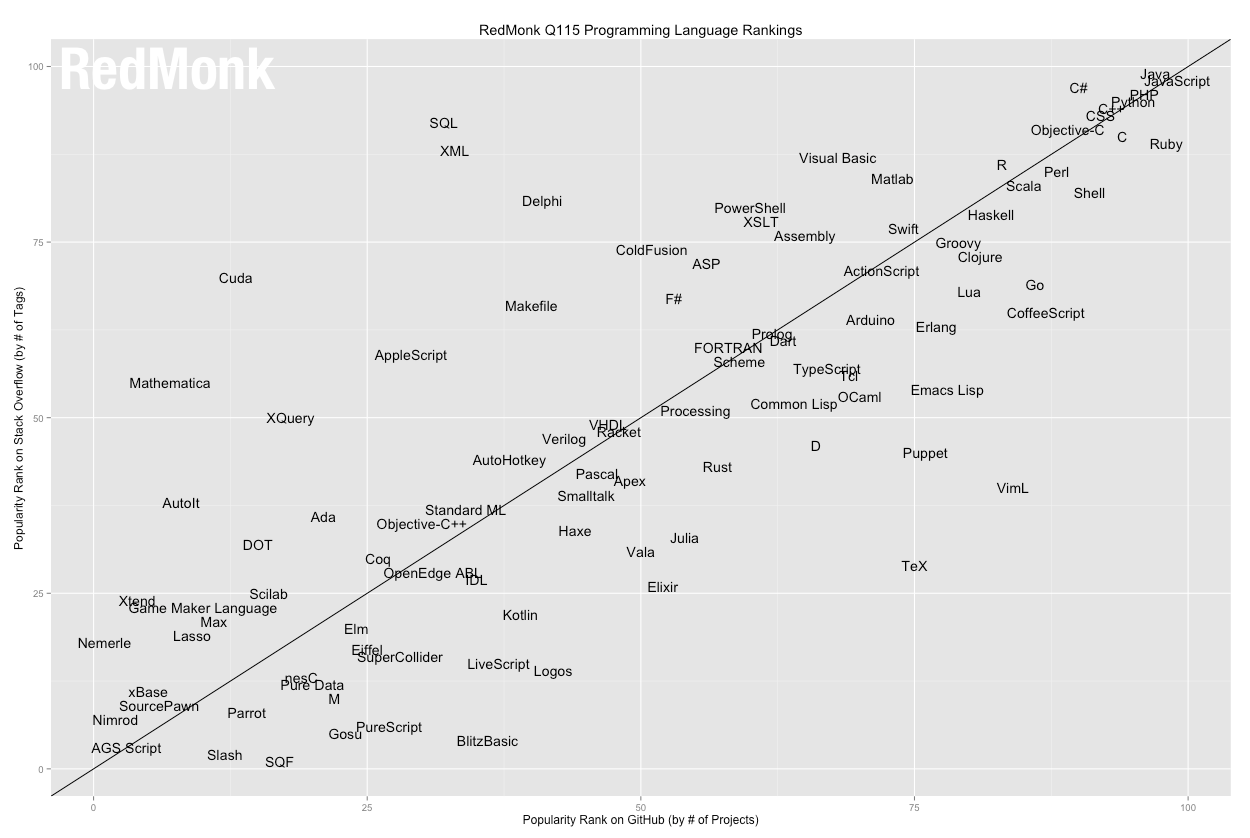
\includegraphics[width=1\textwidth]{img/grafico_redmonk}
	\caption{Ranking das liguagens de programação no Stack Overflow e Github}
\end{figure}


Ainda assim, para compor a interface do dado projeto, também ocorrerá o uso do líder JavaScript de forma intensa, provendo o elo com o as informações gerenciadas pelo PHP.


Entretanto, não seria inteligente desenvolver um sistema completo sem o auxílio de um framework. Dentre os frameworks disponíveis para PHP, hoje o destaque está com o Laravel, que se encontra no topo dentre os mais utilizados no momento. 


A WebHostFace, uma empresa de hospedagem, compilou várias estatísticas para criar um infográfico mostrando os frameworks PHP mais populares de 2015. Utilizando informações sobre os próprios clientes, o Google Trends, estatísticas de repositórios do GitHub e a pesquisa do SitePoint “Best PHP Frameworks 2015”, a WebHostFace elaborou o seguinte infográfico: 

\begin{figure}
	\label{fig:graficoWebhostface}
	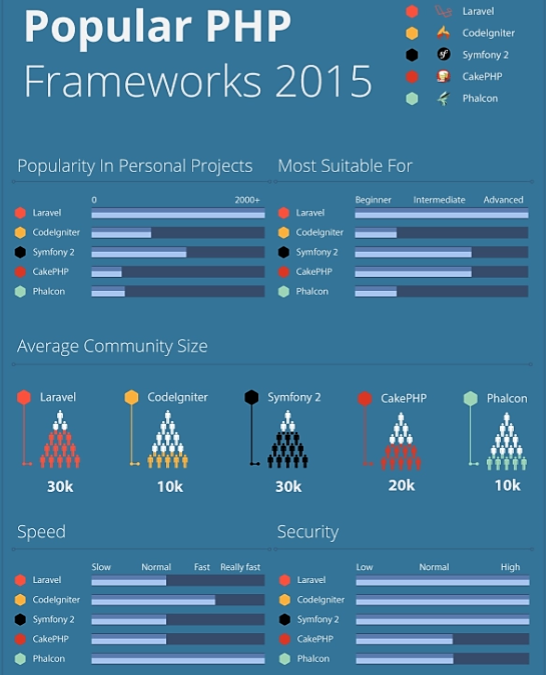
\includegraphics[width=1\textwidth]{img/infografico_webhostface}
	\caption{Infográfico da WebhostFace, exibindo a popularidade dos Frameworks PHP em 2015}
\end{figure}

Assim, tem-se a evidência que o Laravel em 2015 teve a maior popularidade em projetos pessoais e tem a maior comunidade entre os concorrentes, o que o torna uma boa escolha para a escrita de um software que será continuado por terceiros.


Para elaborar os recursos de interface e integrar ao back-end PHP do sistema, será adotado o já conhecido AngularJS, ferramenta sólida e conhecida no aspecto em questão. 


Dados coletados via Google Trends, que propõe comparações entre termos pesquisados, revela a popularidade do AngularJs diante de alguns dos principais concorrentes. O gráfico abaixo evidencia o cenário.


%Como mostra a Figura \ref{fig:graficoGoogleTrendsFerramentasFront}. 
\begin{figure}
	\label{fig:graficoGoogleTrendsFerramentasFront}
	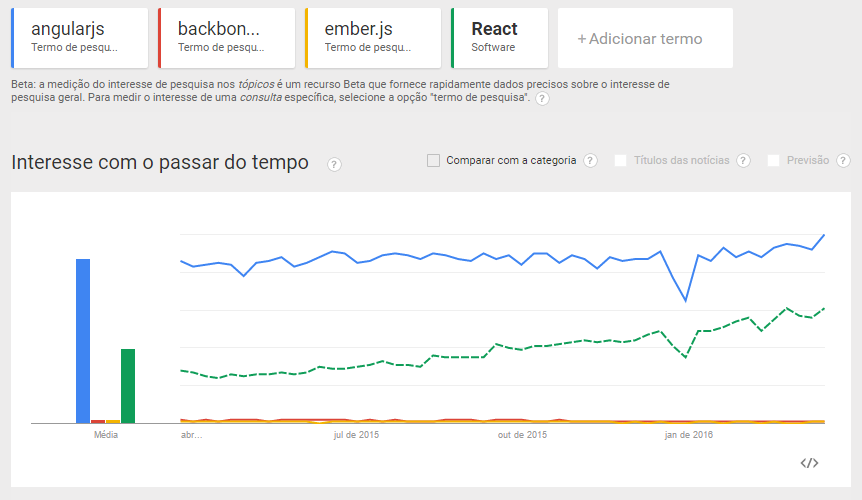
\includegraphics[width=1\textwidth]{img/grafico_ferramentas_front}
	\caption{Gráfico do Google Trends exibindo as pesquisas por ferramentas front-end}
\end{figure}


Junto ao Angular JS, será utilizada a agradável tendência de interface do Material Design da Google, que propõe layouts limpos e otimizados já conhecidos pelos usuários de smartphones Android. 


Para a elaboração da plataforma mobile do projeto, será utilizado o Ionic Framework, muito difundido e bastante pesquisado na área, o que fica evidenciado com o gráfico de pesquisbaixo, coletado via Google Trends buscando por frameworks de desenvolvimento híbrido mobile.


\begin{figure}
	\label{fig:graficoGoogleTrendsFerramentasHibridasMobile}
	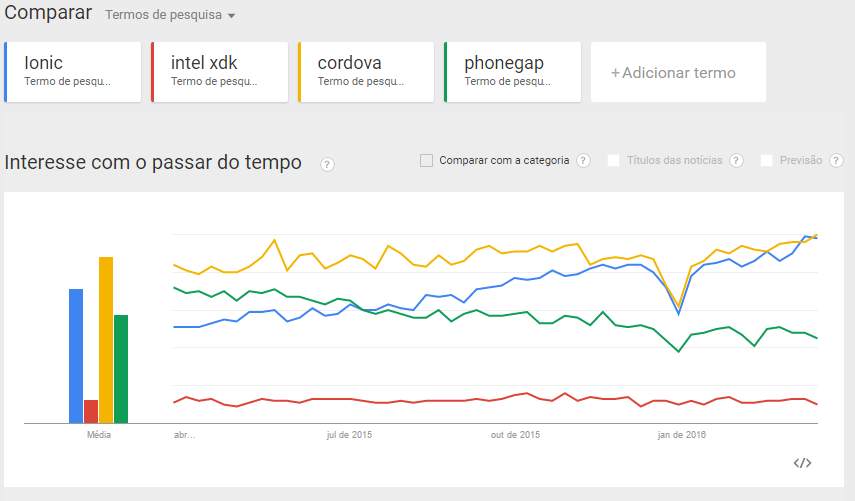
\includegraphics[width=1\textwidth]{img/grafico_ferramentas_hibridas_mobile}
	\caption{Gráfico do Google Trends exibindo as pesquisas por Frameworks híbridos mobile}
\end{figure}	

Para layout da interface mobile, também será aplicado a tendência do Material Design, a fim de propor uma harmonia entre o módulo web e mobile para os usuários


\section{Resultados Esperados}


Como fruto de um sistema para pós-graduação da UFBA, espera-se que os professores tenham mais recursos para integrar as atividades e também prover melhores condições para acompanhamento da vida acadêmica dos alunos em questão. Também, que os novos colaboradores que entrarem no processo tenham facilidade de compreender o fluxo do setor ao navegar pelo sistema proposto.


\section{Fora de Escopo}


Interação com os alunos devido às complicações para realizar a integração com o sistema empregado na UFBA, gerenciado pela XXXXXX, o que causaria uma inviabilidade no projeto devido à necessidade de entrega do produto ser mais forte que o tempo necessário para executar o processo de obtenção de acesso ao sistema legado para realizar a integração.


\section{Estrutura do Trabalho}


<breve resumo sobre os capítulos do TCC>
\chapter{Referencial Teórico}


Projetar o desenvolvimento de um software requer muito planejamento, pois as falhas iniciais podem custar bastante caro ou até mesmo inviabilizar a continuação de um projeto. Assim, a escolha da arquitetura ideal para a aplicabilidade é essencial na concepção de um produto de software. 
De todo o modo, sempre busca-se fazer mais com menos. Diante de tal filosofia, temos nesta seção, uma breve discussão sobre alguns elementos de projeto e arquitetura de software, a fim de contextualizar este trabalho de conclusão de curso.


% Ser direto no começo, focando no que realmente será discutido A seção \ref{sec:apps_mobile} 
 \section{Software como serviço}\label{sec:saas}


A definição de SaaS encontra-se muito bem elaborada em um dos trabalhos listados na literatura. Segundo La e Chun \citep{La2009Systematic}, o princípio da definição de Software como um Serviço (Sofware as a Service - SaaS) é um serviço complementar para aplicações da computação em nuvem (cloud computing). As duas áreas estão interligadas, no entanto, não se confundem, pois o SaaS deve ser entendido como um mecanismo de suporte às soluções existentes na cloud. Os SaaS existem justamente para maximizar o reuso de serviços repetidos e não centrais em uma aplicação remota.


Como propõe vantagens, software como servico é uma tendência forte, isso graças à evolução da web. Diversos fatores podem ser favoráveis para a adoção de um SaaS, como custo e manutenção dentre outros fatores aplicaveis a determinados contextos. Um trabalho recente realizado por Lechessa et al. \cite{LechesaSS11} apresenta uma pesquisa qualitativa sobre os fatores determinantes para adoção ou não de um SaaS voltado para ERP na África do Sul. Esses autores indicam que os principais fatores determinantes para adoção desse mecanismo de software são sua fluidez quanto à rede e a segurança. Esses fatores estão presentes na aplicação desenvolvida neste trabalho de conclusão de curso.
 

Devido ao fato de ter um serviço constantemente na nuvem, fica o questionamento sobre a segurança da informação manipulada. Sabe-se que a vulnerabilidade na web não é restrita ao SaaS, atingindo diversos âmbitos. O artigo de Rai et al. \cite{journals/corr/RaiSM13} orienta como o avanço da computação em nuvem não é um problema apenas para os serviços web do ponto de vista da segurança, pois muitos trabalhos na literatura mostram a área como mais um ponto de vulnerabilidade para diversos setores, a exemplo de infraestrutura. No mesmo artigo mencionado de Rai et al. \cite{journals/corr/RaiSM13}, também realizaram-se estudos exploratórios junto a empresas usuárias de serviços em computação em nuvem e consideram que a perspectiva de SaaS também pode fortalecer a segurança nas aplicações de cloud computing, pois o software de autenticação compartilhado por várias aplicações em nuvem, oferece uma melhor padronização e consequente facilidade de prevenção a erros de vulnerabilidade específicas de cada módulo da pesquisa. Esse ponto de vista é muito importante para qualquer trabalho de ponta na área de SaaS.


A arquitetura de armazenamento de dados de um Saas pode variar de acordo com a necessidade do contexto. O artigo recente de Huixin \cite{7586486}, exemplifica possíveis modelagens para utilizar. Tal abordagem pode ser com um banco de dados único, fazendo com que diferentes clientes compartilhem o mesmo banco, diferindo os dados através de controle de usuário, ou isolando os diferentes clientes através de bancos de dados exclusivos para cada um. Tal fator também pode ser combinado com a arquitetura da aplicação, caso ofereça aplicação única para todos os clientes ou aplicação compartilhada. Diante das possíveis abprdagens, a modelagem de dados do software pode ser decidida pela regra de negócio. Este trabalho optou por aplicação única e banco de dados compartilhado.


Devido ao diferente conceito de obtenção de software, tanto pela visão do cliente como pela visão do vendedor, é necessário tomar conhecimento dos diversos fatores que podem ser relevantes ao orçar um Saas. O recente trabalho de T. Kaur et al. \citep{6949281} orienta um modelo para compor o custo de um Saas. O custo total seria composto pelos fatores que dão suporte ao funcionamento do software. Tais fatores incluem infra-estrutura, configurabilidade, customização, parâmetros de QoS(Quality of service) como escalabilidade, disponibilidade, usabilidade, pontualidade e desempenho da resposta, portabilidade, custo total de propriedade e retorno do investimento. Esses fatores caracterizam o custo de forma eficaz, possibilitando ao fornecedor, prover um Serviço de acordo com a exigência do consumidor em vários pacotes de serviços.


\section{Reuso de software}\label{sec:reuso} %CRUISE BOOK CAPITULO 2


Para Peter Freeman, o reuso é a utilização de qualquer informação que um desenvolvedor pode necessitar no processo de criação de software (Ezran et al., 2002). Basili e Rombach definem reutilização de software como o uso de tudo o que está associado a um projeto de conhecimento (Basili e Rombach, 1991).
Assim, o objetivo da reutilização de software é reciclar o design, código e outros componentes de um produto de software e assim reduzir o custo, o tempo e melhorar a qualidade do produto.
Segundo Keswani et al. \cite{6783445}, o componente reutilizável de software pode ser qualquer parte de seu desenvolvimento, como um fragmento de código, design, casos de teste, ou até mesmo a especificação de requisitos de uma funcionalidade do software. 

O reuso de software pode ter impacto positivo em diversos aspectos do software, vejamos alguns, conforme apresentados no C.R.U.I.S.E Book:

\begin{itemize}

\item Qualidade: As correções de erro tornam-se úteis em todos os locais em que ocorreu, padronizando e facilitando a manutenção.

\item Produtividade: O ganho de produtividade é alcançado devido ao menor número de artefatos desenvolvido. Isso resulta em menos esforços de teste e também economiza análise e design, gerando economia em diversos escopos do projeto.

\item Confiabilidade: A utilização de componentes bem testados aumenta a
confiança no software. Além disso, a utilização de um mesmo componente em vários sistemas, aumenta a possibilidade de detecção de erros e reforça a confiança no componente.

\item Redução do Esforço: A reutilização de software proporciona uma redução do tempo de desenvolvimento, o que reduz o tempo necessário para o produto ser disponibilizado no mercado para trazer rentabilidade.

\item Trabalho redundante e tempo de desenvolvimento: Desenvolver um sistema do
zero significa desenvolvimento redundante de muitos componentes, como requisito
especificações, casos de uso, arquitetura, etc. Isso pode ser evitado quando estes estão disponíveis como componentes reutilizáveis e podem ser compartilhados, resultando em menos desenvolvimento, tempo e custo associado.

\item Documentação: Embora a documentação seja muito importante para a
manutenção de um sistema, muitas vezes é negligenciada. A reutilização de componentes software reduz a quantidade de documentação a ser escrita, entretanto depende da qualidade do que está escrito. Assim, apenas a estrutura do sistema e os novos artefatos desenvolvidos necessitam ser documentados.

\item Custo de manutenção: Menos defeitos e manutenções são esperados quando tem-se comprovada a qualidade dos componentes utilizados.

\item Tamanho da equipe: É comum entrar casos em que a equipe de desenvolvimento sofre sobrecarga. Entretanto, dobrar o tamanho da equipe de desenvolvimento não necessariamente duplica produtividade. Se muitos componentes podem ser reutilizados, é possível desenvolver com equipes menores, levando a melhores comunicações e aumento da produtividade.

\end{itemize}

Apesar dos benefícios da reutilização de software, a mesma não é amplamente praticado como imagina-se. Existem fatores que influenciam direta ou indiretamente na sua adoção. Esses fatores podem ser de aspecto gerencial, organizacional, econômico, conceitual ou técnico. Veremos a seguir alguns aspectos que podem gerar conflito com a cultura de reuso de software, segundo o C.R.U.I.S.E Book:
%(Sametinger, 1997). REVER

\begin{itemize}
	
\item Falta de apoio da gestão: Como a reutilização de software gera custos iniciais,
a medida pode não ser amplamente alcançada em uma organização sem o apoio de alto nível gestão. Os gestores têm de ser informados sobre os custos iniciais e serem convencidos sobre economias futuras.

\item Gerenciamento do Projeto: Gerenciar projetos tradicionais é uma tarefa árdua, principalmente, os que praticam a reutilização de software. Utilizando a técnica em larga escala, tem-se impacto sobre todo o ciclo de vida do software.

\item Estruturas organizacionais inadequadas: As estruturas organizacionais devem
considerar diferentes necessidades que surgem quando a reutilização em larga escala está sendo adotada. Por exemplo, uma equipe particionada pode ser alocada somente para desenvolver, manter e certificar componentes reutilizáveis de software.

\item Incentivos de gestão: É comum a falta de incentivo para deixar os desenvolvedores gastarem tempo elaborando reutilizáveis componentes do sistema. A produtividade é muitas vezes medida apenas no tempo necessário para concluir um projeto. Assim, fazer qualquer trabalho além disso, embora benéfico para a empresa como um todo, diminui o seu sucesso. Mesmo quando os componentes reutilizáveis são utilizados, os benefícios obtidos são uma pequena fração do que poderia ser alcançado caso houvesse reutilização explícita, planejada e organizada.

\item Dificuldade de encontrar software reutilizável: Para reutilizar os componentes, devem existir formas eficientes de busca. Além disso, é importante ter um repositório bem organizado contendo componentes com um eficiente meio de acesso.

\item Não reutilização do software encontrado. O acesso fácil ao software existente
não necessariamente aumentar a reutilização. Os componentes reutilizáveis devem ser cuidadosamente especificados, projetados, implementados e documentados, pois em alguns casos, modificar e adaptar o código  pode ser mais custoso que a programação da funcionalidade necessária a partir do zero.

\item Modificação: É muito difícil encontrar um componente que funcione
exatamente da mesma maneira que queremos. Desta forma, são necessárias modificações e devem existir formas de determinar os seus efeitos sobre o componente.


\end{itemize}


%Outra diretriz importante para a reutilização de software é reduzir o risco na criação de novos softwares. O risco tende a ser bastante reduzido se os componentes que estão sendo reutilizados têm as documentação, interfaces necessárias e devidamente testadas, fatores que contibruem para uma fácil integração.
%De acordo com Keswani et al. \citep{6783445}, para o reuso de software dar retornos apropriados, o processo deve ser sistemático e planejado. Qualquer organização que implemente a reutilização de software deve identificar os melhores métodos e estratégias de reutilização para obter a máxima produtividade. A reutilização de software ajuda a evitar software de engenharia a partir do zero, pois usa módulos de software existentes. A reutilização de software, embora seja uma tarefa difícil, especialmente para softwares antigos sem padrões de projeto, pode melhorar significativamente a produtividade e a qualidade de um produto de software. Embora a reutilização de software não seja um novo campo, ela pode dar grandes retornos em curto período de tempo.


\section{Modularização}\label{sec:modularizacao} %artigo de claudio pagina 222 introdução


%A modularidade vem desempenhando um papel predominante estágios emergentes das disciplinas de arquitetura de software [13]. Engenheiros de software consideram modularidade como princípio base na comparação entre arquiteturas alternativas  e arquitetura degeneração [9]. De fato, os engenheiros de software são incentivados a arquitecturas, baseando-se numa multiplicidade de mecanismos de modularidade disponíveis em: 
%(i) Linguagens de descrição de arquitetura (ADLs), como ACME [8], 
%(ii) catálogos de arquitetônicos [2, 13], e 
%(iii) conhecem bem princípios de alto nível, como interfaces de componentes estreitos, acoplamento arquitectónico reduzido e semelhantes.


Conforme é frisado no trabalho de Wickramaarachchi e Lai \citep{7062705}, o conceito de modularização na indústria de software tem uma longa história e tem sido utilizado para melhorar o processo de desenvolvimento de software em diferentes estágios. Os principais conceitos por trás da modularização do software foram introduzidos por pesquisadores pioneiros há quarenta anos, com uma notável contribuição feita por Melvin Conway e David Parnas, que tem representação notável na engenharia de software.


Modularizar um software é um bom padrão a ser adotado. Segundo Wickramaarachchi e Lai \citep{7062705}, a modularização é importante na identificação de dependências e reduz as dificuldades diante de uma possível necessidade de grandes alterações. De uma perspectiva da engenharia de software, uma modularização geralmente tem várias vantagens, tais como: tornar a complexidade do software mais gerenciável, facilitar o trabalho paralelo e tornar o software mais maleável para acomodar o futuro incerto que um software pode ter. O objetivo final da modularização do software é aumentar a produtividade ea qualidade do software. Tal conceito encontra-se bastante difundido e estái incorporado em linguagens de programação e ferramentas de software. O trabalho proposto favorece ao uso da modularização de um software e até mesmo pode ser considerado um módulo a ser acoplado a qualquer software, mediante a compatibilidade.


\section{Aplicações web}\label{sec:apps_web}


A popularidade da aplicação web aumentou exponencialmente na última década e todos os dias cresce o número de pessoas usuárias de aplicações web. E seguindo o padrão de desenvolvimento de software, Kumar et al. \citep{7813710} sugerem que para o desenvolvimento web, deve-se manter a prática efiacaz de produzir diagramas UML. A abordagem baseada na web oferece uma maneira fácil e eficaz para gerenciar e controlar o processo de desenvolvimento por meio de diagramas UML. Tal abordagem pode ser usada quando há uma exigência de lidar com mudanças muito rápidas e grandes em requisitos de forma muito eficaz em muito menos tempo, gerando assim um menor impacto. 


Para atender à fomentada demanda de aplicativos web, é necessário adotar métodos de desenvolvimentos que sejam ágeis, eficientes e de fácil manutenção. Yu Ping et al. \cite{1372143} propõem o uso do modelo MVC (Model, View e Controller) no atual desenvolvimento para softwares web. O modelo apresentado tornou-se um padrão popular e divide o software em camadas com propósito definido, tornando-o de mais fácil manutenção.


O Ajax (Asynchronous Javascript and XML) revolucionou a web. Conforme demonstrado no artigo de Yuping \citep{6845605}, ao usar a tecnologia Ajax, podemos enriquecer a experiência do usuário em aplicações baseadas em navegador de internet, e fornecer uma variedade de aplicações interativas para atender às necessidade de humanização das aplicações.
Os aplicativos Ajax em execução no navegador se comunicam com um servidor Web de forma assíncrona e atualizam apenas uma parte da página.



% %% RiSE Latex Template - version 0.5
%%
%% RiSE's latex template for thesis and dissertations
%% http://risetemplate.sourceforge.net
%%
%% (c) 2012 Yguaratã Cerqueira Cavalcanti (yguarata@gmail.com)
%%          Vinicius Cardoso Garcia (vinicius.garcia@gmail.com)
%%
%% This document was initially based on UFPEThesis template, from Paulo Gustavo
%% S. Fonseca.
%%
%% ACKNOWLEDGEMENTS
%%
%% We would like to thanks the RiSE's researchers community, the 
%% students from Federal University of Pernambuco, and other users that have
%% been contributing to this projects with comments and patches.
%%
%% GENERAL INSTRUCTIONS
%%
%% We strongly recommend you to compile your documents using pdflatex command.
%% It is also recommend use the texlipse plugin for Eclipse to edit your documents.
%%
%% Options for \documentclass command:
%%         * Idiom
%%           pt   - Portguese (default)
%%           en   - English
%%
%%         * Text type
%%           bsc  - B.Sc. Thesis
%%           msc  - M.Sc. Thesis (default)
%%           qual - PHD qualification (not tested yet)
%%           prop - PHD proposal (not tested yet)
%%           phd  - PHD thesis
%%
%%         * Media
%%           scr  - to eletronic version (PDF) / see the users guide
%%
%%         * Pagination
%%           oneside - unique face press
%%           twoside - two faces press
%%
%%		   * Line spacing
%%           singlespacing  - the same as using \linespread{1}
%%           onehalfspacing - the same as using \linespread{1.3}
%%           doublespacing  - the same as using \linespread{1.6}
%%
%% Reference commands. Use the following commands to make references in your
%% text:
%%          \figref  -- for Figure reference
%%          \tabref  -- for Table reference
%%          \eqnref  -- for equation reference
%%          \chapref -- for chapter reference
%%          \secref  -- for section reference
%%          \appref  -- for appendix reference
%%          \axiref  -- for axiom reference
%%          \conjref -- for conjecture reference
%%          \defref  -- for definition reference
%%          \lemref  -- for lemma reference
%%          \theoref -- for theorem reference
%%          \corref  -- for corollary reference
%%          \propref -- for proprosition reference
%%          \pgref   -- for page reference
%%
%%          Example: See \chapref{chap:introduction}. It will produce 
%%                   'See Chapter 1', in case of English language.

\documentclass[pt,twoside,onehalfspacing,bsc]{risethesis}

\usepackage[utf8]{inputenc}
\usepackage[brazilian]{babel}
\usepackage[T1]{fontenc}

%% Change the following pdf author attribute name to your name.
\usepackage[linkcolor=blue,citecolor=blue,urlcolor=blue,colorlinks,pdfpagelabels,pdftitle={Bruno Cabral's Bachelor Thesis},pdfauthor={Bruno Cabral}]{hyperref}

\address{SALVADOR}

\universitypt{Universidade Federal da Bahia}
\universityen{Federal University of Bahia}

\departmentpt{Depertamento de Ciência da Computação}
\departmenten{Computer Science Department}

\programpt{Programa Multiinstitucional de Pós-graduação em Ciência da Computação}
\programen{Graduate in Computer Science}

\majorfieldpt{Ciência da Computação}
\majorfielden{Computer Science}

\title{Sistema de apoio à Pós graduação - UFBA}
\date{Outubro/2016}

\author{Victor de Azevedo Nunes}
\adviser{Ivan do Carmo Machado}

\begin{document}

\frontmatter
\frontpage
\presentationpage

\begin{dedicatory}
Eu dedico esta dissertação...
%I dedicate this dissertation to my family, girlfriend, friends and
%professors who gave me all necessary support to get here.
\end{dedicatory}

\acknowledgements
Meus agradecimentos...

\begin{epigraph}[]{Edward V Berard}
Walking on water and developing software from a specification are easy if both are frozen
\end{epigraph}

\resumo
% Escreva seu resumo no arquivo resumo.tex
\input{resumo}

\abstract
% Write your abstract in a file called abstract.tex
\input{abstract}

% Summary (tables of contents)
\tableofcontents

% List of figures
\listoffigures

% List of tables
\listoftables

% List of acronyms
% Acronyms manual: http://linorg.usp.br/CTAN/macros/latex/contrib/acronym/acronym.pdf
\listofacronyms
\input{acronyms}

% List of listings
%\lstlistoflistings

\mainmatter

\include{chapters/intro}
\include{chapters/referencial_teorico}

% \include{chapters/introduction/main}
% \include{chapters/background/main}
% \include{chapters/proposed_solution/main}
% \include{chapters/experiment/main}
% \include{chapters/conclusion/main}

\bibliographystyle{natbib}
\addcontentsline{toc}{chapter}{\bibliographytocname}
\bibliography{references}

% Appendix
\clearpage
\addappheadtotoc
\appendix
\appendixpage
% \include{appendix/experiment-instruments}

\end{document}
% %% RiSE Latex Template - version 0.5
%%
%% RiSE's latex template for thesis and dissertations
%% http://risetemplate.sourceforge.net
%%
%% (c) 2012 Yguaratã Cerqueira Cavalcanti (yguarata@gmail.com)
%%          Vinicius Cardoso Garcia (vinicius.garcia@gmail.com)
%%
%% This document was initially based on UFPEThesis template, from Paulo Gustavo
%% S. Fonseca.
%%
%% ACKNOWLEDGEMENTS
%%
%% We would like to thanks the RiSE's researchers community, the 
%% students from Federal University of Pernambuco, and other users that have
%% been contributing to this projects with comments and patches.
%%
%% GENERAL INSTRUCTIONS
%%
%% We strongly recommend you to compile your documents using pdflatex command.
%% It is also recommend use the texlipse plugin for Eclipse to edit your documents.
%%
%% Options for \documentclass command:
%%         * Idiom
%%           pt   - Portguese (default)
%%           en   - English
%%
%%         * Text type
%%           bsc  - B.Sc. Thesis
%%           msc  - M.Sc. Thesis (default)
%%           qual - PHD qualification (not tested yet)
%%           prop - PHD proposal (not tested yet)
%%           phd  - PHD thesis
%%
%%         * Media
%%           scr  - to eletronic version (PDF) / see the users guide
%%
%%         * Pagination
%%           oneside - unique face press
%%           twoside - two faces press
%%
%%		   * Line spacing
%%           singlespacing  - the same as using \linespread{1}
%%           onehalfspacing - the same as using \linespread{1.3}
%%           doublespacing  - the same as using \linespread{1.6}
%%
%% Reference commands. Use the following commands to make references in your
%% text:
%%          \figref  -- for Figure reference
%%          \tabref  -- for Table reference
%%          \eqnref  -- for equation reference
%%          \chapref -- for chapter reference
%%          \secref  -- for section reference
%%          \appref  -- for appendix reference
%%          \axiref  -- for axiom reference
%%          \conjref -- for conjecture reference
%%          \defref  -- for definition reference
%%          \lemref  -- for lemma reference
%%          \theoref -- for theorem reference
%%          \corref  -- for corollary reference
%%          \propref -- for proprosition reference
%%          \pgref   -- for page reference
%%
%%          Example: See \chapref{chap:introduction}. It will produce 
%%                   'See Chapter 1', in case of English language.

\documentclass[pt,twoside,onehalfspacing,bsc]{risethesis}

\usepackage[utf8]{inputenc}
\usepackage[brazilian]{babel}
\usepackage[T1]{fontenc}

%% Change the following pdf author attribute name to your name.
\usepackage[linkcolor=blue,citecolor=blue,urlcolor=blue,colorlinks,pdfpagelabels,pdftitle={Bruno Cabral's Bachelor Thesis},pdfauthor={Bruno Cabral}]{hyperref}

\address{SALVADOR}

\universitypt{Universidade Federal da Bahia}
\universityen{Federal University of Bahia}

\departmentpt{Depertamento de Ciência da Computação}
\departmenten{Computer Science Department}

\programpt{Programa Multiinstitucional de Pós-graduação em Ciência da Computação}
\programen{Graduate in Computer Science}

\majorfieldpt{Ciência da Computação}
\majorfielden{Computer Science}

\title{Sistema de apoio à Pós graduação - UFBA}
\date{Outubro/2016}

\author{Victor de Azevedo Nunes}
\adviser{Ivan do Carmo Machado}

\begin{document}

\frontmatter
\frontpage
\presentationpage

\begin{dedicatory}
Eu dedico esta dissertação...
%I dedicate this dissertation to my family, girlfriend, friends and
%professors who gave me all necessary support to get here.
\end{dedicatory}

\acknowledgements
Meus agradecimentos...

\begin{epigraph}[]{Edward V Berard}
Walking on water and developing software from a specification are easy if both are frozen
\end{epigraph}

\resumo
% Escreva seu resumo no arquivo resumo.tex
\input{resumo}

\abstract
% Write your abstract in a file called abstract.tex
\input{abstract}

% Summary (tables of contents)
\tableofcontents

% List of figures
\listoffigures

% List of tables
\listoftables

% List of acronyms
% Acronyms manual: http://linorg.usp.br/CTAN/macros/latex/contrib/acronym/acronym.pdf
\listofacronyms
\input{acronyms}

% List of listings
%\lstlistoflistings

\mainmatter

\include{chapters/intro}
\include{chapters/referencial_teorico}

% \include{chapters/introduction/main}
% \include{chapters/background/main}
% \include{chapters/proposed_solution/main}
% \include{chapters/experiment/main}
% \include{chapters/conclusion/main}

\bibliographystyle{natbib}
\addcontentsline{toc}{chapter}{\bibliographytocname}
\bibliography{references}

% Appendix
\clearpage
\addappheadtotoc
\appendix
\appendixpage
% \include{appendix/experiment-instruments}

\end{document}
% %% RiSE Latex Template - version 0.5
%%
%% RiSE's latex template for thesis and dissertations
%% http://risetemplate.sourceforge.net
%%
%% (c) 2012 Yguaratã Cerqueira Cavalcanti (yguarata@gmail.com)
%%          Vinicius Cardoso Garcia (vinicius.garcia@gmail.com)
%%
%% This document was initially based on UFPEThesis template, from Paulo Gustavo
%% S. Fonseca.
%%
%% ACKNOWLEDGEMENTS
%%
%% We would like to thanks the RiSE's researchers community, the 
%% students from Federal University of Pernambuco, and other users that have
%% been contributing to this projects with comments and patches.
%%
%% GENERAL INSTRUCTIONS
%%
%% We strongly recommend you to compile your documents using pdflatex command.
%% It is also recommend use the texlipse plugin for Eclipse to edit your documents.
%%
%% Options for \documentclass command:
%%         * Idiom
%%           pt   - Portguese (default)
%%           en   - English
%%
%%         * Text type
%%           bsc  - B.Sc. Thesis
%%           msc  - M.Sc. Thesis (default)
%%           qual - PHD qualification (not tested yet)
%%           prop - PHD proposal (not tested yet)
%%           phd  - PHD thesis
%%
%%         * Media
%%           scr  - to eletronic version (PDF) / see the users guide
%%
%%         * Pagination
%%           oneside - unique face press
%%           twoside - two faces press
%%
%%		   * Line spacing
%%           singlespacing  - the same as using \linespread{1}
%%           onehalfspacing - the same as using \linespread{1.3}
%%           doublespacing  - the same as using \linespread{1.6}
%%
%% Reference commands. Use the following commands to make references in your
%% text:
%%          \figref  -- for Figure reference
%%          \tabref  -- for Table reference
%%          \eqnref  -- for equation reference
%%          \chapref -- for chapter reference
%%          \secref  -- for section reference
%%          \appref  -- for appendix reference
%%          \axiref  -- for axiom reference
%%          \conjref -- for conjecture reference
%%          \defref  -- for definition reference
%%          \lemref  -- for lemma reference
%%          \theoref -- for theorem reference
%%          \corref  -- for corollary reference
%%          \propref -- for proprosition reference
%%          \pgref   -- for page reference
%%
%%          Example: See \chapref{chap:introduction}. It will produce 
%%                   'See Chapter 1', in case of English language.

\documentclass[pt,twoside,onehalfspacing,bsc]{risethesis}

\usepackage[utf8]{inputenc}
\usepackage[brazilian]{babel}
\usepackage[T1]{fontenc}

%% Change the following pdf author attribute name to your name.
\usepackage[linkcolor=blue,citecolor=blue,urlcolor=blue,colorlinks,pdfpagelabels,pdftitle={Bruno Cabral's Bachelor Thesis},pdfauthor={Bruno Cabral}]{hyperref}

\address{SALVADOR}

\universitypt{Universidade Federal da Bahia}
\universityen{Federal University of Bahia}

\departmentpt{Depertamento de Ciência da Computação}
\departmenten{Computer Science Department}

\programpt{Programa Multiinstitucional de Pós-graduação em Ciência da Computação}
\programen{Graduate in Computer Science}

\majorfieldpt{Ciência da Computação}
\majorfielden{Computer Science}

\title{Sistema de apoio à Pós graduação - UFBA}
\date{Outubro/2016}

\author{Victor de Azevedo Nunes}
\adviser{Ivan do Carmo Machado}

\begin{document}

\frontmatter
\frontpage
\presentationpage

\begin{dedicatory}
Eu dedico esta dissertação...
%I dedicate this dissertation to my family, girlfriend, friends and
%professors who gave me all necessary support to get here.
\end{dedicatory}

\acknowledgements
Meus agradecimentos...

\begin{epigraph}[]{Edward V Berard}
Walking on water and developing software from a specification are easy if both are frozen
\end{epigraph}

\resumo
% Escreva seu resumo no arquivo resumo.tex
\input{resumo}

\abstract
% Write your abstract in a file called abstract.tex
\input{abstract}

% Summary (tables of contents)
\tableofcontents

% List of figures
\listoffigures

% List of tables
\listoftables

% List of acronyms
% Acronyms manual: http://linorg.usp.br/CTAN/macros/latex/contrib/acronym/acronym.pdf
\listofacronyms
\input{acronyms}

% List of listings
%\lstlistoflistings

\mainmatter

\include{chapters/intro}
\include{chapters/referencial_teorico}

% \include{chapters/introduction/main}
% \include{chapters/background/main}
% \include{chapters/proposed_solution/main}
% \include{chapters/experiment/main}
% \include{chapters/conclusion/main}

\bibliographystyle{natbib}
\addcontentsline{toc}{chapter}{\bibliographytocname}
\bibliography{references}

% Appendix
\clearpage
\addappheadtotoc
\appendix
\appendixpage
% \include{appendix/experiment-instruments}

\end{document}
% %% RiSE Latex Template - version 0.5
%%
%% RiSE's latex template for thesis and dissertations
%% http://risetemplate.sourceforge.net
%%
%% (c) 2012 Yguaratã Cerqueira Cavalcanti (yguarata@gmail.com)
%%          Vinicius Cardoso Garcia (vinicius.garcia@gmail.com)
%%
%% This document was initially based on UFPEThesis template, from Paulo Gustavo
%% S. Fonseca.
%%
%% ACKNOWLEDGEMENTS
%%
%% We would like to thanks the RiSE's researchers community, the 
%% students from Federal University of Pernambuco, and other users that have
%% been contributing to this projects with comments and patches.
%%
%% GENERAL INSTRUCTIONS
%%
%% We strongly recommend you to compile your documents using pdflatex command.
%% It is also recommend use the texlipse plugin for Eclipse to edit your documents.
%%
%% Options for \documentclass command:
%%         * Idiom
%%           pt   - Portguese (default)
%%           en   - English
%%
%%         * Text type
%%           bsc  - B.Sc. Thesis
%%           msc  - M.Sc. Thesis (default)
%%           qual - PHD qualification (not tested yet)
%%           prop - PHD proposal (not tested yet)
%%           phd  - PHD thesis
%%
%%         * Media
%%           scr  - to eletronic version (PDF) / see the users guide
%%
%%         * Pagination
%%           oneside - unique face press
%%           twoside - two faces press
%%
%%		   * Line spacing
%%           singlespacing  - the same as using \linespread{1}
%%           onehalfspacing - the same as using \linespread{1.3}
%%           doublespacing  - the same as using \linespread{1.6}
%%
%% Reference commands. Use the following commands to make references in your
%% text:
%%          \figref  -- for Figure reference
%%          \tabref  -- for Table reference
%%          \eqnref  -- for equation reference
%%          \chapref -- for chapter reference
%%          \secref  -- for section reference
%%          \appref  -- for appendix reference
%%          \axiref  -- for axiom reference
%%          \conjref -- for conjecture reference
%%          \defref  -- for definition reference
%%          \lemref  -- for lemma reference
%%          \theoref -- for theorem reference
%%          \corref  -- for corollary reference
%%          \propref -- for proprosition reference
%%          \pgref   -- for page reference
%%
%%          Example: See \chapref{chap:introduction}. It will produce 
%%                   'See Chapter 1', in case of English language.

\documentclass[pt,twoside,onehalfspacing,bsc]{risethesis}

\usepackage[utf8]{inputenc}
\usepackage[brazilian]{babel}
\usepackage[T1]{fontenc}

%% Change the following pdf author attribute name to your name.
\usepackage[linkcolor=blue,citecolor=blue,urlcolor=blue,colorlinks,pdfpagelabels,pdftitle={Bruno Cabral's Bachelor Thesis},pdfauthor={Bruno Cabral}]{hyperref}

\address{SALVADOR}

\universitypt{Universidade Federal da Bahia}
\universityen{Federal University of Bahia}

\departmentpt{Depertamento de Ciência da Computação}
\departmenten{Computer Science Department}

\programpt{Programa Multiinstitucional de Pós-graduação em Ciência da Computação}
\programen{Graduate in Computer Science}

\majorfieldpt{Ciência da Computação}
\majorfielden{Computer Science}

\title{Sistema de apoio à Pós graduação - UFBA}
\date{Outubro/2016}

\author{Victor de Azevedo Nunes}
\adviser{Ivan do Carmo Machado}

\begin{document}

\frontmatter
\frontpage
\presentationpage

\begin{dedicatory}
Eu dedico esta dissertação...
%I dedicate this dissertation to my family, girlfriend, friends and
%professors who gave me all necessary support to get here.
\end{dedicatory}

\acknowledgements
Meus agradecimentos...

\begin{epigraph}[]{Edward V Berard}
Walking on water and developing software from a specification are easy if both are frozen
\end{epigraph}

\resumo
% Escreva seu resumo no arquivo resumo.tex
\input{resumo}

\abstract
% Write your abstract in a file called abstract.tex
\input{abstract}

% Summary (tables of contents)
\tableofcontents

% List of figures
\listoffigures

% List of tables
\listoftables

% List of acronyms
% Acronyms manual: http://linorg.usp.br/CTAN/macros/latex/contrib/acronym/acronym.pdf
\listofacronyms
\input{acronyms}

% List of listings
%\lstlistoflistings

\mainmatter

\include{chapters/intro}
\include{chapters/referencial_teorico}

% \include{chapters/introduction/main}
% \include{chapters/background/main}
% \include{chapters/proposed_solution/main}
% \include{chapters/experiment/main}
% \include{chapters/conclusion/main}

\bibliographystyle{natbib}
\addcontentsline{toc}{chapter}{\bibliographytocname}
\bibliography{references}

% Appendix
\clearpage
\addappheadtotoc
\appendix
\appendixpage
% \include{appendix/experiment-instruments}

\end{document}
% %% RiSE Latex Template - version 0.5
%%
%% RiSE's latex template for thesis and dissertations
%% http://risetemplate.sourceforge.net
%%
%% (c) 2012 Yguaratã Cerqueira Cavalcanti (yguarata@gmail.com)
%%          Vinicius Cardoso Garcia (vinicius.garcia@gmail.com)
%%
%% This document was initially based on UFPEThesis template, from Paulo Gustavo
%% S. Fonseca.
%%
%% ACKNOWLEDGEMENTS
%%
%% We would like to thanks the RiSE's researchers community, the 
%% students from Federal University of Pernambuco, and other users that have
%% been contributing to this projects with comments and patches.
%%
%% GENERAL INSTRUCTIONS
%%
%% We strongly recommend you to compile your documents using pdflatex command.
%% It is also recommend use the texlipse plugin for Eclipse to edit your documents.
%%
%% Options for \documentclass command:
%%         * Idiom
%%           pt   - Portguese (default)
%%           en   - English
%%
%%         * Text type
%%           bsc  - B.Sc. Thesis
%%           msc  - M.Sc. Thesis (default)
%%           qual - PHD qualification (not tested yet)
%%           prop - PHD proposal (not tested yet)
%%           phd  - PHD thesis
%%
%%         * Media
%%           scr  - to eletronic version (PDF) / see the users guide
%%
%%         * Pagination
%%           oneside - unique face press
%%           twoside - two faces press
%%
%%		   * Line spacing
%%           singlespacing  - the same as using \linespread{1}
%%           onehalfspacing - the same as using \linespread{1.3}
%%           doublespacing  - the same as using \linespread{1.6}
%%
%% Reference commands. Use the following commands to make references in your
%% text:
%%          \figref  -- for Figure reference
%%          \tabref  -- for Table reference
%%          \eqnref  -- for equation reference
%%          \chapref -- for chapter reference
%%          \secref  -- for section reference
%%          \appref  -- for appendix reference
%%          \axiref  -- for axiom reference
%%          \conjref -- for conjecture reference
%%          \defref  -- for definition reference
%%          \lemref  -- for lemma reference
%%          \theoref -- for theorem reference
%%          \corref  -- for corollary reference
%%          \propref -- for proprosition reference
%%          \pgref   -- for page reference
%%
%%          Example: See \chapref{chap:introduction}. It will produce 
%%                   'See Chapter 1', in case of English language.

\documentclass[pt,twoside,onehalfspacing,bsc]{risethesis}

\usepackage[utf8]{inputenc}
\usepackage[brazilian]{babel}
\usepackage[T1]{fontenc}

%% Change the following pdf author attribute name to your name.
\usepackage[linkcolor=blue,citecolor=blue,urlcolor=blue,colorlinks,pdfpagelabels,pdftitle={Bruno Cabral's Bachelor Thesis},pdfauthor={Bruno Cabral}]{hyperref}

\address{SALVADOR}

\universitypt{Universidade Federal da Bahia}
\universityen{Federal University of Bahia}

\departmentpt{Depertamento de Ciência da Computação}
\departmenten{Computer Science Department}

\programpt{Programa Multiinstitucional de Pós-graduação em Ciência da Computação}
\programen{Graduate in Computer Science}

\majorfieldpt{Ciência da Computação}
\majorfielden{Computer Science}

\title{Sistema de apoio à Pós graduação - UFBA}
\date{Outubro/2016}

\author{Victor de Azevedo Nunes}
\adviser{Ivan do Carmo Machado}

\begin{document}

\frontmatter
\frontpage
\presentationpage

\begin{dedicatory}
Eu dedico esta dissertação...
%I dedicate this dissertation to my family, girlfriend, friends and
%professors who gave me all necessary support to get here.
\end{dedicatory}

\acknowledgements
Meus agradecimentos...

\begin{epigraph}[]{Edward V Berard}
Walking on water and developing software from a specification are easy if both are frozen
\end{epigraph}

\resumo
% Escreva seu resumo no arquivo resumo.tex
\input{resumo}

\abstract
% Write your abstract in a file called abstract.tex
\input{abstract}

% Summary (tables of contents)
\tableofcontents

% List of figures
\listoffigures

% List of tables
\listoftables

% List of acronyms
% Acronyms manual: http://linorg.usp.br/CTAN/macros/latex/contrib/acronym/acronym.pdf
\listofacronyms
\input{acronyms}

% List of listings
%\lstlistoflistings

\mainmatter

\include{chapters/intro}
\include{chapters/referencial_teorico}

% \include{chapters/introduction/main}
% \include{chapters/background/main}
% \include{chapters/proposed_solution/main}
% \include{chapters/experiment/main}
% \include{chapters/conclusion/main}

\bibliographystyle{natbib}
\addcontentsline{toc}{chapter}{\bibliographytocname}
\bibliography{references}

% Appendix
\clearpage
\addappheadtotoc
\appendix
\appendixpage
% \include{appendix/experiment-instruments}

\end{document}

\bibliographystyle{natbib}
\addcontentsline{toc}{chapter}{\bibliographytocname}
\bibliography{references}

% Appendix
\clearpage
\addappheadtotoc
\appendix
\appendixpage
% \include{appendix/experiment-instruments}

\end{document}
% %% RiSE Latex Template - version 0.5
%%
%% RiSE's latex template for thesis and dissertations
%% http://risetemplate.sourceforge.net
%%
%% (c) 2012 Yguaratã Cerqueira Cavalcanti (yguarata@gmail.com)
%%          Vinicius Cardoso Garcia (vinicius.garcia@gmail.com)
%%
%% This document was initially based on UFPEThesis template, from Paulo Gustavo
%% S. Fonseca.
%%
%% ACKNOWLEDGEMENTS
%%
%% We would like to thanks the RiSE's researchers community, the 
%% students from Federal University of Pernambuco, and other users that have
%% been contributing to this projects with comments and patches.
%%
%% GENERAL INSTRUCTIONS
%%
%% We strongly recommend you to compile your documents using pdflatex command.
%% It is also recommend use the texlipse plugin for Eclipse to edit your documents.
%%
%% Options for \documentclass command:
%%         * Idiom
%%           pt   - Portguese (default)
%%           en   - English
%%
%%         * Text type
%%           bsc  - B.Sc. Thesis
%%           msc  - M.Sc. Thesis (default)
%%           qual - PHD qualification (not tested yet)
%%           prop - PHD proposal (not tested yet)
%%           phd  - PHD thesis
%%
%%         * Media
%%           scr  - to eletronic version (PDF) / see the users guide
%%
%%         * Pagination
%%           oneside - unique face press
%%           twoside - two faces press
%%
%%		   * Line spacing
%%           singlespacing  - the same as using \linespread{1}
%%           onehalfspacing - the same as using \linespread{1.3}
%%           doublespacing  - the same as using \linespread{1.6}
%%
%% Reference commands. Use the following commands to make references in your
%% text:
%%          \figref  -- for Figure reference
%%          \tabref  -- for Table reference
%%          \eqnref  -- for equation reference
%%          \chapref -- for chapter reference
%%          \secref  -- for section reference
%%          \appref  -- for appendix reference
%%          \axiref  -- for axiom reference
%%          \conjref -- for conjecture reference
%%          \defref  -- for definition reference
%%          \lemref  -- for lemma reference
%%          \theoref -- for theorem reference
%%          \corref  -- for corollary reference
%%          \propref -- for proprosition reference
%%          \pgref   -- for page reference
%%
%%          Example: See \chapref{chap:introduction}. It will produce 
%%                   'See Chapter 1', in case of English language.

\documentclass[pt,twoside,onehalfspacing,bsc]{risethesis}

\usepackage[utf8]{inputenc}
\usepackage[brazilian]{babel}
\usepackage[T1]{fontenc}

%% Change the following pdf author attribute name to your name.
\usepackage[linkcolor=blue,citecolor=blue,urlcolor=blue,colorlinks,pdfpagelabels,pdftitle={Bruno Cabral's Bachelor Thesis},pdfauthor={Bruno Cabral}]{hyperref}

\address{SALVADOR}

\universitypt{Universidade Federal da Bahia}
\universityen{Federal University of Bahia}

\departmentpt{Depertamento de Ciência da Computação}
\departmenten{Computer Science Department}

\programpt{Programa Multiinstitucional de Pós-graduação em Ciência da Computação}
\programen{Graduate in Computer Science}

\majorfieldpt{Ciência da Computação}
\majorfielden{Computer Science}

\title{Sistema de apoio à Pós graduação - UFBA}
\date{Outubro/2016}

\author{Victor de Azevedo Nunes}
\adviser{Ivan do Carmo Machado}

\begin{document}

\frontmatter
\frontpage
\presentationpage

\begin{dedicatory}
Eu dedico esta dissertação...
%I dedicate this dissertation to my family, girlfriend, friends and
%professors who gave me all necessary support to get here.
\end{dedicatory}

\acknowledgements
Meus agradecimentos...

\begin{epigraph}[]{Edward V Berard}
Walking on water and developing software from a specification are easy if both are frozen
\end{epigraph}

\resumo
% Escreva seu resumo no arquivo resumo.tex
Meu resumo

\begin{keywords}
palavras chave

\end{keywords}

\abstract
% Write your abstract in a file called abstract.tex
My abstract...

\begin{keywords}
key words...
\end{keywords}

% Summary (tables of contents)
\tableofcontents

% List of figures
\listoffigures

% List of tables
\listoftables

% List of acronyms
% Acronyms manual: http://linorg.usp.br/CTAN/macros/latex/contrib/acronym/acronym.pdf
\listofacronyms
\begin{acronym}[ACRONYM] 
% Change the word ACRONYM above to change the acronym column width.
% The column width is equals to the width of the word that you put.
% Read the manual about acronym package for more examples:
%   http://linorg.usp.br/CTAN/macros/latex/contrib/acronym/acronym.pdf

\acro{SPA}{Single Page Application}
\acro{JSON}{Javascript Object Notation}
\acro{PHP}{PHP: Hypertext Preprocessor}
\acro{SaaS}{Software as a Service}
\acro{ERP}{Enterprise Resource Planning}
\acro{QoS}{Quality of Service}
\acro{UML}{Unified Modeling Language}
\acro{MVC}{Model-View-Controller}
\acro{Ajax}{Asynchronous Javascript and XML}
\acro{HTML}{HyperText Markup Language}
\acro{CSS}{Cascading Style Sheets}
\acro{API}{Application Programming Interface}
\acro{DOM}{Document Object Model}
\acro{BPMN}{Business Process Model and Notation}
\acro{REST}{Representational State Transfer}

\end{acronym}

% List of listings
%\lstlistoflistings

\mainmatter

\chapter{Introdução}

\section{Motivação}

Organizar os procedimentos de um processo sempre nos traz vantagens. Apesar de no processo de implantação de um sistema, o mesmo burocratizar o processo, com o tempo temos o retorno da dedicação para a inserção dos dados. Com um certo volume de dados, é possível estruturar informações que num processo manual são difíceis de serem enxergadas. Assim, é possível depender menos das pessoas que organizam o processo, pois o legado de informações não estará mais somente na mente de alguns, mas sim documentado nos dados do sistema.

Além de colaborar na organização, também haverá uma grande colaboração no tempo gasto na gestão. Lidar com muitos papéis e confiar na mente humana para guardar informações, não é uma alternativa muito segura devido ao fato que as pessoas sempre estão sujeitas a sair do processo e levar contigo a experiência obtida. Experiência essa que faz com que os procedimentos sejam executados de forma mais eficiente. Entretanto, com um sistema inteligente, é possível auxiliar e tornar mais ágil a execução das tarefas.


\section{Problema}


De acordo com funcionários ligados ao o setor de pós graduação da UFBA, entrevistados a fim de um maior entendimento do cenário, apesar das semelhanças estruturais, a pós graduação gerida de forma diferencia da graduação. FULANO afirma que devido ao fato de não ter a mesma visibilidade, não tem acesso aos mesmos recursos de gestão acadêmica da graduação. O professores não executam somente atividades dentro da sala de aula, também tem diversas outras ocupações no setor. E muitos procedimentos realizados extra classe ainda se encontram sendo realizados de forma manual, estando mais vulnerável ao erro ou até mesmo à violação do processo. Também ocorre um grande desperdício de tempo pelos professores e gestores da área, devido ao diversos processos ainda realizados de forma manual, sem a devida documentação. Segundo FULANO, também entrevistado, esse tempo perdido implica numa redução da eficiência na sala de aula, pois o professor acaba por ter menos tempo disponível para o planejamento das atividades, o que gera impactos negativos aos alunos.


\section{Objetivos} %<o que deve ser feito/entregue>


Devido aos muitos processos sendo resolvidos de forma manual, propõe-se com solução um sistema moderno, arquitetado para ter funcionamento na web e com um módulo mobile, a fim de fornecer informações de forma rápida e eficiente para os professores através de notificações, já que o acesso à internet móvel é comum entre os possíveis usuários do sistema em questão.
O principal requisito para o sistema seria dispor recursos para reduzir o tempo desperdiçado pelos professores durante as atividades extra classe.


\section{Metodologia} %<como será feito | como resolver o problema apontado inicialmente>


%<analise de literatura | design | implementação | validação>
Baseando-se nas tecnologias gratuitas em alta no cenário atual do desenvolvimento web, dispomos de algumas opções eficientes para a implementação da solução. Dentre as possibilidades, considerando a facilidade para futura manutenção e continuidade do projeto, tende-se a optar por uma tecnologia popular. Como linguagem de programação, adota-se o PHP. A escolha é fundamentada de acordo com a pesquisa da RedMonk de 2015, que evidencia o uso das linguagens de programação de acordo com as discussões no StackOverflow e repositórios no GitHub. É possível constatar a popularidade do PHP no cenário atual com o gráfico da pesquisa citada, na qual o PHP é apresentado na terceira colocação, apenas atrás do lider JavaScript e do segundo colocado, o Java.

\begin{figure}
	\label{fig:graficoRedmonk}
	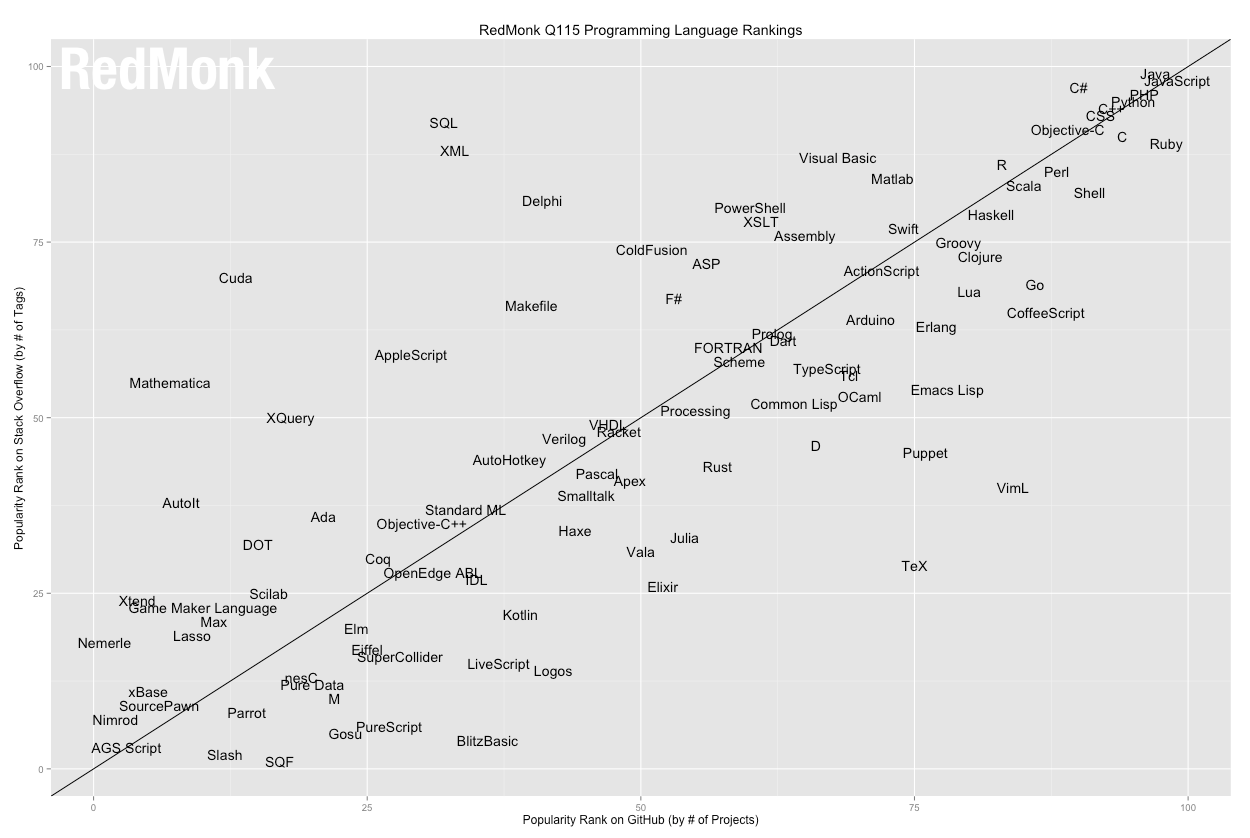
\includegraphics[width=1\textwidth]{img/grafico_redmonk}
	\caption{Ranking das liguagens de programação no Stack Overflow e Github}
\end{figure}


Ainda assim, para compor a interface do dado projeto, também ocorrerá o uso do líder JavaScript de forma intensa, provendo o elo com o as informações gerenciadas pelo PHP.


Entretanto, não seria inteligente desenvolver um sistema completo sem o auxílio de um framework. Dentre os frameworks disponíveis para PHP, hoje o destaque está com o Laravel, que se encontra no topo dentre os mais utilizados no momento. 


A WebHostFace, uma empresa de hospedagem, compilou várias estatísticas para criar um infográfico mostrando os frameworks PHP mais populares de 2015. Utilizando informações sobre os próprios clientes, o Google Trends, estatísticas de repositórios do GitHub e a pesquisa do SitePoint “Best PHP Frameworks 2015”, a WebHostFace elaborou o seguinte infográfico: 

\begin{figure}
	\label{fig:graficoWebhostface}
	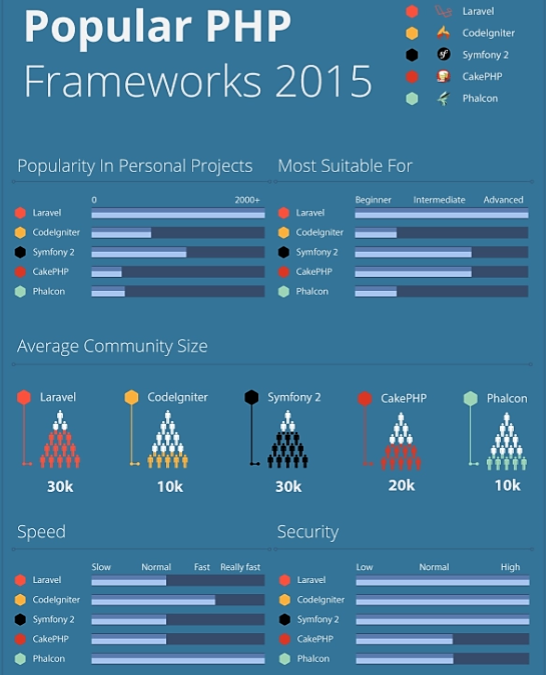
\includegraphics[width=1\textwidth]{img/infografico_webhostface}
	\caption{Infográfico da WebhostFace, exibindo a popularidade dos Frameworks PHP em 2015}
\end{figure}

Assim, tem-se a evidência que o Laravel em 2015 teve a maior popularidade em projetos pessoais e tem a maior comunidade entre os concorrentes, o que o torna uma boa escolha para a escrita de um software que será continuado por terceiros.


Para elaborar os recursos de interface e integrar ao back-end PHP do sistema, será adotado o já conhecido AngularJS, ferramenta sólida e conhecida no aspecto em questão. 


Dados coletados via Google Trends, que propõe comparações entre termos pesquisados, revela a popularidade do AngularJs diante de alguns dos principais concorrentes. O gráfico abaixo evidencia o cenário.


%Como mostra a Figura \ref{fig:graficoGoogleTrendsFerramentasFront}. 
\begin{figure}
	\label{fig:graficoGoogleTrendsFerramentasFront}
	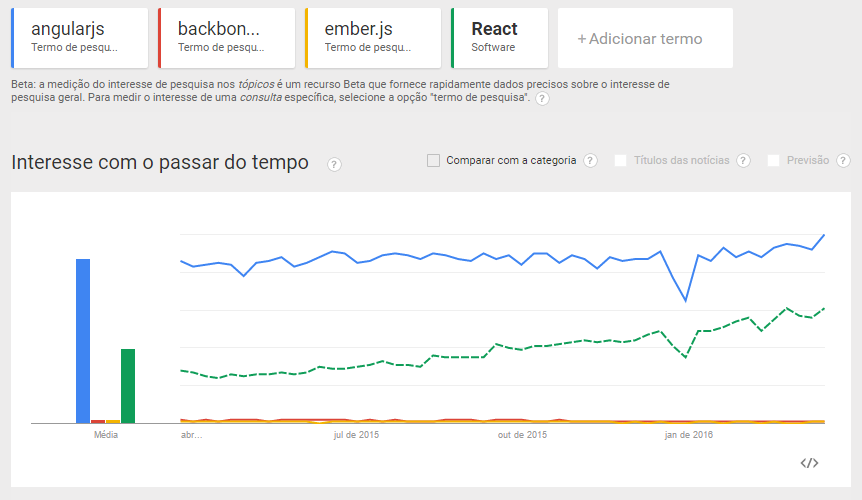
\includegraphics[width=1\textwidth]{img/grafico_ferramentas_front}
	\caption{Gráfico do Google Trends exibindo as pesquisas por ferramentas front-end}
\end{figure}


Junto ao Angular JS, será utilizada a agradável tendência de interface do Material Design da Google, que propõe layouts limpos e otimizados já conhecidos pelos usuários de smartphones Android. 


Para a elaboração da plataforma mobile do projeto, será utilizado o Ionic Framework, muito difundido e bastante pesquisado na área, o que fica evidenciado com o gráfico de pesquisbaixo, coletado via Google Trends buscando por frameworks de desenvolvimento híbrido mobile.


\begin{figure}
	\label{fig:graficoGoogleTrendsFerramentasHibridasMobile}
	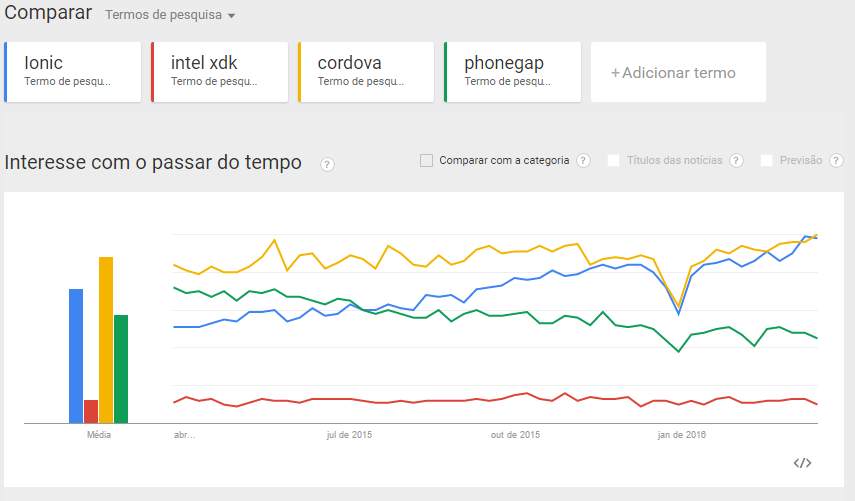
\includegraphics[width=1\textwidth]{img/grafico_ferramentas_hibridas_mobile}
	\caption{Gráfico do Google Trends exibindo as pesquisas por Frameworks híbridos mobile}
\end{figure}	

Para layout da interface mobile, também será aplicado a tendência do Material Design, a fim de propor uma harmonia entre o módulo web e mobile para os usuários


\section{Resultados Esperados}


Como fruto de um sistema para pós-graduação da UFBA, espera-se que os professores tenham mais recursos para integrar as atividades e também prover melhores condições para acompanhamento da vida acadêmica dos alunos em questão. Também, que os novos colaboradores que entrarem no processo tenham facilidade de compreender o fluxo do setor ao navegar pelo sistema proposto.


\section{Fora de Escopo}


Interação com os alunos devido às complicações para realizar a integração com o sistema empregado na UFBA, gerenciado pela XXXXXX, o que causaria uma inviabilidade no projeto devido à necessidade de entrega do produto ser mais forte que o tempo necessário para executar o processo de obtenção de acesso ao sistema legado para realizar a integração.


\section{Estrutura do Trabalho}


<breve resumo sobre os capítulos do TCC>
\chapter{Referencial Teórico}


Projetar o desenvolvimento de um software requer muito planejamento, pois as falhas iniciais podem custar bastante caro ou até mesmo inviabilizar a continuação de um projeto. Assim, a escolha da arquitetura ideal para a aplicabilidade é essencial na concepção de um produto de software. 
De todo o modo, sempre busca-se fazer mais com menos. Diante de tal filosofia, temos nesta seção, uma breve discussão sobre alguns elementos de projeto e arquitetura de software, a fim de contextualizar este trabalho de conclusão de curso.


% Ser direto no começo, focando no que realmente será discutido A seção \ref{sec:apps_mobile} 
 \section{Software como serviço}\label{sec:saas}


A definição de SaaS encontra-se muito bem elaborada em um dos trabalhos listados na literatura. Segundo La e Chun \citep{La2009Systematic}, o princípio da definição de Software como um Serviço (Sofware as a Service - SaaS) é um serviço complementar para aplicações da computação em nuvem (cloud computing). As duas áreas estão interligadas, no entanto, não se confundem, pois o SaaS deve ser entendido como um mecanismo de suporte às soluções existentes na cloud. Os SaaS existem justamente para maximizar o reuso de serviços repetidos e não centrais em uma aplicação remota.


Como propõe vantagens, software como servico é uma tendência forte, isso graças à evolução da web. Diversos fatores podem ser favoráveis para a adoção de um SaaS, como custo e manutenção dentre outros fatores aplicaveis a determinados contextos. Um trabalho recente realizado por Lechessa et al. \cite{LechesaSS11} apresenta uma pesquisa qualitativa sobre os fatores determinantes para adoção ou não de um SaaS voltado para ERP na África do Sul. Esses autores indicam que os principais fatores determinantes para adoção desse mecanismo de software são sua fluidez quanto à rede e a segurança. Esses fatores estão presentes na aplicação desenvolvida neste trabalho de conclusão de curso.
 

Devido ao fato de ter um serviço constantemente na nuvem, fica o questionamento sobre a segurança da informação manipulada. Sabe-se que a vulnerabilidade na web não é restrita ao SaaS, atingindo diversos âmbitos. O artigo de Rai et al. \cite{journals/corr/RaiSM13} orienta como o avanço da computação em nuvem não é um problema apenas para os serviços web do ponto de vista da segurança, pois muitos trabalhos na literatura mostram a área como mais um ponto de vulnerabilidade para diversos setores, a exemplo de infraestrutura. No mesmo artigo mencionado de Rai et al. \cite{journals/corr/RaiSM13}, também realizaram-se estudos exploratórios junto a empresas usuárias de serviços em computação em nuvem e consideram que a perspectiva de SaaS também pode fortalecer a segurança nas aplicações de cloud computing, pois o software de autenticação compartilhado por várias aplicações em nuvem, oferece uma melhor padronização e consequente facilidade de prevenção a erros de vulnerabilidade específicas de cada módulo da pesquisa. Esse ponto de vista é muito importante para qualquer trabalho de ponta na área de SaaS.


A arquitetura de armazenamento de dados de um Saas pode variar de acordo com a necessidade do contexto. O artigo recente de Huixin \cite{7586486}, exemplifica possíveis modelagens para utilizar. Tal abordagem pode ser com um banco de dados único, fazendo com que diferentes clientes compartilhem o mesmo banco, diferindo os dados através de controle de usuário, ou isolando os diferentes clientes através de bancos de dados exclusivos para cada um. Tal fator também pode ser combinado com a arquitetura da aplicação, caso ofereça aplicação única para todos os clientes ou aplicação compartilhada. Diante das possíveis abprdagens, a modelagem de dados do software pode ser decidida pela regra de negócio. Este trabalho optou por aplicação única e banco de dados compartilhado.


Devido ao diferente conceito de obtenção de software, tanto pela visão do cliente como pela visão do vendedor, é necessário tomar conhecimento dos diversos fatores que podem ser relevantes ao orçar um Saas. O recente trabalho de T. Kaur et al. \citep{6949281} orienta um modelo para compor o custo de um Saas. O custo total seria composto pelos fatores que dão suporte ao funcionamento do software. Tais fatores incluem infra-estrutura, configurabilidade, customização, parâmetros de QoS(Quality of service) como escalabilidade, disponibilidade, usabilidade, pontualidade e desempenho da resposta, portabilidade, custo total de propriedade e retorno do investimento. Esses fatores caracterizam o custo de forma eficaz, possibilitando ao fornecedor, prover um Serviço de acordo com a exigência do consumidor em vários pacotes de serviços.


\section{Reuso de software}\label{sec:reuso} %CRUISE BOOK CAPITULO 2


Para Peter Freeman, o reuso é a utilização de qualquer informação que um desenvolvedor pode necessitar no processo de criação de software (Ezran et al., 2002). Basili e Rombach definem reutilização de software como o uso de tudo o que está associado a um projeto de conhecimento (Basili e Rombach, 1991).
Assim, o objetivo da reutilização de software é reciclar o design, código e outros componentes de um produto de software e assim reduzir o custo, o tempo e melhorar a qualidade do produto.
Segundo Keswani et al. \cite{6783445}, o componente reutilizável de software pode ser qualquer parte de seu desenvolvimento, como um fragmento de código, design, casos de teste, ou até mesmo a especificação de requisitos de uma funcionalidade do software. 

O reuso de software pode ter impacto positivo em diversos aspectos do software, vejamos alguns, conforme apresentados no C.R.U.I.S.E Book:

\begin{itemize}

\item Qualidade: As correções de erro tornam-se úteis em todos os locais em que ocorreu, padronizando e facilitando a manutenção.

\item Produtividade: O ganho de produtividade é alcançado devido ao menor número de artefatos desenvolvido. Isso resulta em menos esforços de teste e também economiza análise e design, gerando economia em diversos escopos do projeto.

\item Confiabilidade: A utilização de componentes bem testados aumenta a
confiança no software. Além disso, a utilização de um mesmo componente em vários sistemas, aumenta a possibilidade de detecção de erros e reforça a confiança no componente.

\item Redução do Esforço: A reutilização de software proporciona uma redução do tempo de desenvolvimento, o que reduz o tempo necessário para o produto ser disponibilizado no mercado para trazer rentabilidade.

\item Trabalho redundante e tempo de desenvolvimento: Desenvolver um sistema do
zero significa desenvolvimento redundante de muitos componentes, como requisito
especificações, casos de uso, arquitetura, etc. Isso pode ser evitado quando estes estão disponíveis como componentes reutilizáveis e podem ser compartilhados, resultando em menos desenvolvimento, tempo e custo associado.

\item Documentação: Embora a documentação seja muito importante para a
manutenção de um sistema, muitas vezes é negligenciada. A reutilização de componentes software reduz a quantidade de documentação a ser escrita, entretanto depende da qualidade do que está escrito. Assim, apenas a estrutura do sistema e os novos artefatos desenvolvidos necessitam ser documentados.

\item Custo de manutenção: Menos defeitos e manutenções são esperados quando tem-se comprovada a qualidade dos componentes utilizados.

\item Tamanho da equipe: É comum entrar casos em que a equipe de desenvolvimento sofre sobrecarga. Entretanto, dobrar o tamanho da equipe de desenvolvimento não necessariamente duplica produtividade. Se muitos componentes podem ser reutilizados, é possível desenvolver com equipes menores, levando a melhores comunicações e aumento da produtividade.

\end{itemize}

Apesar dos benefícios da reutilização de software, a mesma não é amplamente praticado como imagina-se. Existem fatores que influenciam direta ou indiretamente na sua adoção. Esses fatores podem ser de aspecto gerencial, organizacional, econômico, conceitual ou técnico. Veremos a seguir alguns aspectos que podem gerar conflito com a cultura de reuso de software, segundo o C.R.U.I.S.E Book:
%(Sametinger, 1997). REVER

\begin{itemize}
	
\item Falta de apoio da gestão: Como a reutilização de software gera custos iniciais,
a medida pode não ser amplamente alcançada em uma organização sem o apoio de alto nível gestão. Os gestores têm de ser informados sobre os custos iniciais e serem convencidos sobre economias futuras.

\item Gerenciamento do Projeto: Gerenciar projetos tradicionais é uma tarefa árdua, principalmente, os que praticam a reutilização de software. Utilizando a técnica em larga escala, tem-se impacto sobre todo o ciclo de vida do software.

\item Estruturas organizacionais inadequadas: As estruturas organizacionais devem
considerar diferentes necessidades que surgem quando a reutilização em larga escala está sendo adotada. Por exemplo, uma equipe particionada pode ser alocada somente para desenvolver, manter e certificar componentes reutilizáveis de software.

\item Incentivos de gestão: É comum a falta de incentivo para deixar os desenvolvedores gastarem tempo elaborando reutilizáveis componentes do sistema. A produtividade é muitas vezes medida apenas no tempo necessário para concluir um projeto. Assim, fazer qualquer trabalho além disso, embora benéfico para a empresa como um todo, diminui o seu sucesso. Mesmo quando os componentes reutilizáveis são utilizados, os benefícios obtidos são uma pequena fração do que poderia ser alcançado caso houvesse reutilização explícita, planejada e organizada.

\item Dificuldade de encontrar software reutilizável: Para reutilizar os componentes, devem existir formas eficientes de busca. Além disso, é importante ter um repositório bem organizado contendo componentes com um eficiente meio de acesso.

\item Não reutilização do software encontrado. O acesso fácil ao software existente
não necessariamente aumentar a reutilização. Os componentes reutilizáveis devem ser cuidadosamente especificados, projetados, implementados e documentados, pois em alguns casos, modificar e adaptar o código  pode ser mais custoso que a programação da funcionalidade necessária a partir do zero.

\item Modificação: É muito difícil encontrar um componente que funcione
exatamente da mesma maneira que queremos. Desta forma, são necessárias modificações e devem existir formas de determinar os seus efeitos sobre o componente.


\end{itemize}


%Outra diretriz importante para a reutilização de software é reduzir o risco na criação de novos softwares. O risco tende a ser bastante reduzido se os componentes que estão sendo reutilizados têm as documentação, interfaces necessárias e devidamente testadas, fatores que contibruem para uma fácil integração.
%De acordo com Keswani et al. \citep{6783445}, para o reuso de software dar retornos apropriados, o processo deve ser sistemático e planejado. Qualquer organização que implemente a reutilização de software deve identificar os melhores métodos e estratégias de reutilização para obter a máxima produtividade. A reutilização de software ajuda a evitar software de engenharia a partir do zero, pois usa módulos de software existentes. A reutilização de software, embora seja uma tarefa difícil, especialmente para softwares antigos sem padrões de projeto, pode melhorar significativamente a produtividade e a qualidade de um produto de software. Embora a reutilização de software não seja um novo campo, ela pode dar grandes retornos em curto período de tempo.


\section{Modularização}\label{sec:modularizacao} %artigo de claudio pagina 222 introdução


%A modularidade vem desempenhando um papel predominante estágios emergentes das disciplinas de arquitetura de software [13]. Engenheiros de software consideram modularidade como princípio base na comparação entre arquiteturas alternativas  e arquitetura degeneração [9]. De fato, os engenheiros de software são incentivados a arquitecturas, baseando-se numa multiplicidade de mecanismos de modularidade disponíveis em: 
%(i) Linguagens de descrição de arquitetura (ADLs), como ACME [8], 
%(ii) catálogos de arquitetônicos [2, 13], e 
%(iii) conhecem bem princípios de alto nível, como interfaces de componentes estreitos, acoplamento arquitectónico reduzido e semelhantes.


Conforme é frisado no trabalho de Wickramaarachchi e Lai \citep{7062705}, o conceito de modularização na indústria de software tem uma longa história e tem sido utilizado para melhorar o processo de desenvolvimento de software em diferentes estágios. Os principais conceitos por trás da modularização do software foram introduzidos por pesquisadores pioneiros há quarenta anos, com uma notável contribuição feita por Melvin Conway e David Parnas, que tem representação notável na engenharia de software.


Modularizar um software é um bom padrão a ser adotado. Segundo Wickramaarachchi e Lai \citep{7062705}, a modularização é importante na identificação de dependências e reduz as dificuldades diante de uma possível necessidade de grandes alterações. De uma perspectiva da engenharia de software, uma modularização geralmente tem várias vantagens, tais como: tornar a complexidade do software mais gerenciável, facilitar o trabalho paralelo e tornar o software mais maleável para acomodar o futuro incerto que um software pode ter. O objetivo final da modularização do software é aumentar a produtividade ea qualidade do software. Tal conceito encontra-se bastante difundido e estái incorporado em linguagens de programação e ferramentas de software. O trabalho proposto favorece ao uso da modularização de um software e até mesmo pode ser considerado um módulo a ser acoplado a qualquer software, mediante a compatibilidade.


\section{Aplicações web}\label{sec:apps_web}


A popularidade da aplicação web aumentou exponencialmente na última década e todos os dias cresce o número de pessoas usuárias de aplicações web. E seguindo o padrão de desenvolvimento de software, Kumar et al. \citep{7813710} sugerem que para o desenvolvimento web, deve-se manter a prática efiacaz de produzir diagramas UML. A abordagem baseada na web oferece uma maneira fácil e eficaz para gerenciar e controlar o processo de desenvolvimento por meio de diagramas UML. Tal abordagem pode ser usada quando há uma exigência de lidar com mudanças muito rápidas e grandes em requisitos de forma muito eficaz em muito menos tempo, gerando assim um menor impacto. 


Para atender à fomentada demanda de aplicativos web, é necessário adotar métodos de desenvolvimentos que sejam ágeis, eficientes e de fácil manutenção. Yu Ping et al. \cite{1372143} propõem o uso do modelo MVC (Model, View e Controller) no atual desenvolvimento para softwares web. O modelo apresentado tornou-se um padrão popular e divide o software em camadas com propósito definido, tornando-o de mais fácil manutenção.


O Ajax (Asynchronous Javascript and XML) revolucionou a web. Conforme demonstrado no artigo de Yuping \citep{6845605}, ao usar a tecnologia Ajax, podemos enriquecer a experiência do usuário em aplicações baseadas em navegador de internet, e fornecer uma variedade de aplicações interativas para atender às necessidade de humanização das aplicações.
Os aplicativos Ajax em execução no navegador se comunicam com um servidor Web de forma assíncrona e atualizam apenas uma parte da página.



% %% RiSE Latex Template - version 0.5
%%
%% RiSE's latex template for thesis and dissertations
%% http://risetemplate.sourceforge.net
%%
%% (c) 2012 Yguaratã Cerqueira Cavalcanti (yguarata@gmail.com)
%%          Vinicius Cardoso Garcia (vinicius.garcia@gmail.com)
%%
%% This document was initially based on UFPEThesis template, from Paulo Gustavo
%% S. Fonseca.
%%
%% ACKNOWLEDGEMENTS
%%
%% We would like to thanks the RiSE's researchers community, the 
%% students from Federal University of Pernambuco, and other users that have
%% been contributing to this projects with comments and patches.
%%
%% GENERAL INSTRUCTIONS
%%
%% We strongly recommend you to compile your documents using pdflatex command.
%% It is also recommend use the texlipse plugin for Eclipse to edit your documents.
%%
%% Options for \documentclass command:
%%         * Idiom
%%           pt   - Portguese (default)
%%           en   - English
%%
%%         * Text type
%%           bsc  - B.Sc. Thesis
%%           msc  - M.Sc. Thesis (default)
%%           qual - PHD qualification (not tested yet)
%%           prop - PHD proposal (not tested yet)
%%           phd  - PHD thesis
%%
%%         * Media
%%           scr  - to eletronic version (PDF) / see the users guide
%%
%%         * Pagination
%%           oneside - unique face press
%%           twoside - two faces press
%%
%%		   * Line spacing
%%           singlespacing  - the same as using \linespread{1}
%%           onehalfspacing - the same as using \linespread{1.3}
%%           doublespacing  - the same as using \linespread{1.6}
%%
%% Reference commands. Use the following commands to make references in your
%% text:
%%          \figref  -- for Figure reference
%%          \tabref  -- for Table reference
%%          \eqnref  -- for equation reference
%%          \chapref -- for chapter reference
%%          \secref  -- for section reference
%%          \appref  -- for appendix reference
%%          \axiref  -- for axiom reference
%%          \conjref -- for conjecture reference
%%          \defref  -- for definition reference
%%          \lemref  -- for lemma reference
%%          \theoref -- for theorem reference
%%          \corref  -- for corollary reference
%%          \propref -- for proprosition reference
%%          \pgref   -- for page reference
%%
%%          Example: See \chapref{chap:introduction}. It will produce 
%%                   'See Chapter 1', in case of English language.

\documentclass[pt,twoside,onehalfspacing,bsc]{risethesis}

\usepackage[utf8]{inputenc}
\usepackage[brazilian]{babel}
\usepackage[T1]{fontenc}

%% Change the following pdf author attribute name to your name.
\usepackage[linkcolor=blue,citecolor=blue,urlcolor=blue,colorlinks,pdfpagelabels,pdftitle={Bruno Cabral's Bachelor Thesis},pdfauthor={Bruno Cabral}]{hyperref}

\address{SALVADOR}

\universitypt{Universidade Federal da Bahia}
\universityen{Federal University of Bahia}

\departmentpt{Depertamento de Ciência da Computação}
\departmenten{Computer Science Department}

\programpt{Programa Multiinstitucional de Pós-graduação em Ciência da Computação}
\programen{Graduate in Computer Science}

\majorfieldpt{Ciência da Computação}
\majorfielden{Computer Science}

\title{Sistema de apoio à Pós graduação - UFBA}
\date{Outubro/2016}

\author{Victor de Azevedo Nunes}
\adviser{Ivan do Carmo Machado}

\begin{document}

\frontmatter
\frontpage
\presentationpage

\begin{dedicatory}
Eu dedico esta dissertação...
%I dedicate this dissertation to my family, girlfriend, friends and
%professors who gave me all necessary support to get here.
\end{dedicatory}

\acknowledgements
Meus agradecimentos...

\begin{epigraph}[]{Edward V Berard}
Walking on water and developing software from a specification are easy if both are frozen
\end{epigraph}

\resumo
% Escreva seu resumo no arquivo resumo.tex
\input{resumo}

\abstract
% Write your abstract in a file called abstract.tex
\input{abstract}

% Summary (tables of contents)
\tableofcontents

% List of figures
\listoffigures

% List of tables
\listoftables

% List of acronyms
% Acronyms manual: http://linorg.usp.br/CTAN/macros/latex/contrib/acronym/acronym.pdf
\listofacronyms
\input{acronyms}

% List of listings
%\lstlistoflistings

\mainmatter

\include{chapters/intro}
\include{chapters/referencial_teorico}

% \include{chapters/introduction/main}
% \include{chapters/background/main}
% \include{chapters/proposed_solution/main}
% \include{chapters/experiment/main}
% \include{chapters/conclusion/main}

\bibliographystyle{natbib}
\addcontentsline{toc}{chapter}{\bibliographytocname}
\bibliography{references}

% Appendix
\clearpage
\addappheadtotoc
\appendix
\appendixpage
% \include{appendix/experiment-instruments}

\end{document}
% %% RiSE Latex Template - version 0.5
%%
%% RiSE's latex template for thesis and dissertations
%% http://risetemplate.sourceforge.net
%%
%% (c) 2012 Yguaratã Cerqueira Cavalcanti (yguarata@gmail.com)
%%          Vinicius Cardoso Garcia (vinicius.garcia@gmail.com)
%%
%% This document was initially based on UFPEThesis template, from Paulo Gustavo
%% S. Fonseca.
%%
%% ACKNOWLEDGEMENTS
%%
%% We would like to thanks the RiSE's researchers community, the 
%% students from Federal University of Pernambuco, and other users that have
%% been contributing to this projects with comments and patches.
%%
%% GENERAL INSTRUCTIONS
%%
%% We strongly recommend you to compile your documents using pdflatex command.
%% It is also recommend use the texlipse plugin for Eclipse to edit your documents.
%%
%% Options for \documentclass command:
%%         * Idiom
%%           pt   - Portguese (default)
%%           en   - English
%%
%%         * Text type
%%           bsc  - B.Sc. Thesis
%%           msc  - M.Sc. Thesis (default)
%%           qual - PHD qualification (not tested yet)
%%           prop - PHD proposal (not tested yet)
%%           phd  - PHD thesis
%%
%%         * Media
%%           scr  - to eletronic version (PDF) / see the users guide
%%
%%         * Pagination
%%           oneside - unique face press
%%           twoside - two faces press
%%
%%		   * Line spacing
%%           singlespacing  - the same as using \linespread{1}
%%           onehalfspacing - the same as using \linespread{1.3}
%%           doublespacing  - the same as using \linespread{1.6}
%%
%% Reference commands. Use the following commands to make references in your
%% text:
%%          \figref  -- for Figure reference
%%          \tabref  -- for Table reference
%%          \eqnref  -- for equation reference
%%          \chapref -- for chapter reference
%%          \secref  -- for section reference
%%          \appref  -- for appendix reference
%%          \axiref  -- for axiom reference
%%          \conjref -- for conjecture reference
%%          \defref  -- for definition reference
%%          \lemref  -- for lemma reference
%%          \theoref -- for theorem reference
%%          \corref  -- for corollary reference
%%          \propref -- for proprosition reference
%%          \pgref   -- for page reference
%%
%%          Example: See \chapref{chap:introduction}. It will produce 
%%                   'See Chapter 1', in case of English language.

\documentclass[pt,twoside,onehalfspacing,bsc]{risethesis}

\usepackage[utf8]{inputenc}
\usepackage[brazilian]{babel}
\usepackage[T1]{fontenc}

%% Change the following pdf author attribute name to your name.
\usepackage[linkcolor=blue,citecolor=blue,urlcolor=blue,colorlinks,pdfpagelabels,pdftitle={Bruno Cabral's Bachelor Thesis},pdfauthor={Bruno Cabral}]{hyperref}

\address{SALVADOR}

\universitypt{Universidade Federal da Bahia}
\universityen{Federal University of Bahia}

\departmentpt{Depertamento de Ciência da Computação}
\departmenten{Computer Science Department}

\programpt{Programa Multiinstitucional de Pós-graduação em Ciência da Computação}
\programen{Graduate in Computer Science}

\majorfieldpt{Ciência da Computação}
\majorfielden{Computer Science}

\title{Sistema de apoio à Pós graduação - UFBA}
\date{Outubro/2016}

\author{Victor de Azevedo Nunes}
\adviser{Ivan do Carmo Machado}

\begin{document}

\frontmatter
\frontpage
\presentationpage

\begin{dedicatory}
Eu dedico esta dissertação...
%I dedicate this dissertation to my family, girlfriend, friends and
%professors who gave me all necessary support to get here.
\end{dedicatory}

\acknowledgements
Meus agradecimentos...

\begin{epigraph}[]{Edward V Berard}
Walking on water and developing software from a specification are easy if both are frozen
\end{epigraph}

\resumo
% Escreva seu resumo no arquivo resumo.tex
\input{resumo}

\abstract
% Write your abstract in a file called abstract.tex
\input{abstract}

% Summary (tables of contents)
\tableofcontents

% List of figures
\listoffigures

% List of tables
\listoftables

% List of acronyms
% Acronyms manual: http://linorg.usp.br/CTAN/macros/latex/contrib/acronym/acronym.pdf
\listofacronyms
\input{acronyms}

% List of listings
%\lstlistoflistings

\mainmatter

\include{chapters/intro}
\include{chapters/referencial_teorico}

% \include{chapters/introduction/main}
% \include{chapters/background/main}
% \include{chapters/proposed_solution/main}
% \include{chapters/experiment/main}
% \include{chapters/conclusion/main}

\bibliographystyle{natbib}
\addcontentsline{toc}{chapter}{\bibliographytocname}
\bibliography{references}

% Appendix
\clearpage
\addappheadtotoc
\appendix
\appendixpage
% \include{appendix/experiment-instruments}

\end{document}
% %% RiSE Latex Template - version 0.5
%%
%% RiSE's latex template for thesis and dissertations
%% http://risetemplate.sourceforge.net
%%
%% (c) 2012 Yguaratã Cerqueira Cavalcanti (yguarata@gmail.com)
%%          Vinicius Cardoso Garcia (vinicius.garcia@gmail.com)
%%
%% This document was initially based on UFPEThesis template, from Paulo Gustavo
%% S. Fonseca.
%%
%% ACKNOWLEDGEMENTS
%%
%% We would like to thanks the RiSE's researchers community, the 
%% students from Federal University of Pernambuco, and other users that have
%% been contributing to this projects with comments and patches.
%%
%% GENERAL INSTRUCTIONS
%%
%% We strongly recommend you to compile your documents using pdflatex command.
%% It is also recommend use the texlipse plugin for Eclipse to edit your documents.
%%
%% Options for \documentclass command:
%%         * Idiom
%%           pt   - Portguese (default)
%%           en   - English
%%
%%         * Text type
%%           bsc  - B.Sc. Thesis
%%           msc  - M.Sc. Thesis (default)
%%           qual - PHD qualification (not tested yet)
%%           prop - PHD proposal (not tested yet)
%%           phd  - PHD thesis
%%
%%         * Media
%%           scr  - to eletronic version (PDF) / see the users guide
%%
%%         * Pagination
%%           oneside - unique face press
%%           twoside - two faces press
%%
%%		   * Line spacing
%%           singlespacing  - the same as using \linespread{1}
%%           onehalfspacing - the same as using \linespread{1.3}
%%           doublespacing  - the same as using \linespread{1.6}
%%
%% Reference commands. Use the following commands to make references in your
%% text:
%%          \figref  -- for Figure reference
%%          \tabref  -- for Table reference
%%          \eqnref  -- for equation reference
%%          \chapref -- for chapter reference
%%          \secref  -- for section reference
%%          \appref  -- for appendix reference
%%          \axiref  -- for axiom reference
%%          \conjref -- for conjecture reference
%%          \defref  -- for definition reference
%%          \lemref  -- for lemma reference
%%          \theoref -- for theorem reference
%%          \corref  -- for corollary reference
%%          \propref -- for proprosition reference
%%          \pgref   -- for page reference
%%
%%          Example: See \chapref{chap:introduction}. It will produce 
%%                   'See Chapter 1', in case of English language.

\documentclass[pt,twoside,onehalfspacing,bsc]{risethesis}

\usepackage[utf8]{inputenc}
\usepackage[brazilian]{babel}
\usepackage[T1]{fontenc}

%% Change the following pdf author attribute name to your name.
\usepackage[linkcolor=blue,citecolor=blue,urlcolor=blue,colorlinks,pdfpagelabels,pdftitle={Bruno Cabral's Bachelor Thesis},pdfauthor={Bruno Cabral}]{hyperref}

\address{SALVADOR}

\universitypt{Universidade Federal da Bahia}
\universityen{Federal University of Bahia}

\departmentpt{Depertamento de Ciência da Computação}
\departmenten{Computer Science Department}

\programpt{Programa Multiinstitucional de Pós-graduação em Ciência da Computação}
\programen{Graduate in Computer Science}

\majorfieldpt{Ciência da Computação}
\majorfielden{Computer Science}

\title{Sistema de apoio à Pós graduação - UFBA}
\date{Outubro/2016}

\author{Victor de Azevedo Nunes}
\adviser{Ivan do Carmo Machado}

\begin{document}

\frontmatter
\frontpage
\presentationpage

\begin{dedicatory}
Eu dedico esta dissertação...
%I dedicate this dissertation to my family, girlfriend, friends and
%professors who gave me all necessary support to get here.
\end{dedicatory}

\acknowledgements
Meus agradecimentos...

\begin{epigraph}[]{Edward V Berard}
Walking on water and developing software from a specification are easy if both are frozen
\end{epigraph}

\resumo
% Escreva seu resumo no arquivo resumo.tex
\input{resumo}

\abstract
% Write your abstract in a file called abstract.tex
\input{abstract}

% Summary (tables of contents)
\tableofcontents

% List of figures
\listoffigures

% List of tables
\listoftables

% List of acronyms
% Acronyms manual: http://linorg.usp.br/CTAN/macros/latex/contrib/acronym/acronym.pdf
\listofacronyms
\input{acronyms}

% List of listings
%\lstlistoflistings

\mainmatter

\include{chapters/intro}
\include{chapters/referencial_teorico}

% \include{chapters/introduction/main}
% \include{chapters/background/main}
% \include{chapters/proposed_solution/main}
% \include{chapters/experiment/main}
% \include{chapters/conclusion/main}

\bibliographystyle{natbib}
\addcontentsline{toc}{chapter}{\bibliographytocname}
\bibliography{references}

% Appendix
\clearpage
\addappheadtotoc
\appendix
\appendixpage
% \include{appendix/experiment-instruments}

\end{document}
% %% RiSE Latex Template - version 0.5
%%
%% RiSE's latex template for thesis and dissertations
%% http://risetemplate.sourceforge.net
%%
%% (c) 2012 Yguaratã Cerqueira Cavalcanti (yguarata@gmail.com)
%%          Vinicius Cardoso Garcia (vinicius.garcia@gmail.com)
%%
%% This document was initially based on UFPEThesis template, from Paulo Gustavo
%% S. Fonseca.
%%
%% ACKNOWLEDGEMENTS
%%
%% We would like to thanks the RiSE's researchers community, the 
%% students from Federal University of Pernambuco, and other users that have
%% been contributing to this projects with comments and patches.
%%
%% GENERAL INSTRUCTIONS
%%
%% We strongly recommend you to compile your documents using pdflatex command.
%% It is also recommend use the texlipse plugin for Eclipse to edit your documents.
%%
%% Options for \documentclass command:
%%         * Idiom
%%           pt   - Portguese (default)
%%           en   - English
%%
%%         * Text type
%%           bsc  - B.Sc. Thesis
%%           msc  - M.Sc. Thesis (default)
%%           qual - PHD qualification (not tested yet)
%%           prop - PHD proposal (not tested yet)
%%           phd  - PHD thesis
%%
%%         * Media
%%           scr  - to eletronic version (PDF) / see the users guide
%%
%%         * Pagination
%%           oneside - unique face press
%%           twoside - two faces press
%%
%%		   * Line spacing
%%           singlespacing  - the same as using \linespread{1}
%%           onehalfspacing - the same as using \linespread{1.3}
%%           doublespacing  - the same as using \linespread{1.6}
%%
%% Reference commands. Use the following commands to make references in your
%% text:
%%          \figref  -- for Figure reference
%%          \tabref  -- for Table reference
%%          \eqnref  -- for equation reference
%%          \chapref -- for chapter reference
%%          \secref  -- for section reference
%%          \appref  -- for appendix reference
%%          \axiref  -- for axiom reference
%%          \conjref -- for conjecture reference
%%          \defref  -- for definition reference
%%          \lemref  -- for lemma reference
%%          \theoref -- for theorem reference
%%          \corref  -- for corollary reference
%%          \propref -- for proprosition reference
%%          \pgref   -- for page reference
%%
%%          Example: See \chapref{chap:introduction}. It will produce 
%%                   'See Chapter 1', in case of English language.

\documentclass[pt,twoside,onehalfspacing,bsc]{risethesis}

\usepackage[utf8]{inputenc}
\usepackage[brazilian]{babel}
\usepackage[T1]{fontenc}

%% Change the following pdf author attribute name to your name.
\usepackage[linkcolor=blue,citecolor=blue,urlcolor=blue,colorlinks,pdfpagelabels,pdftitle={Bruno Cabral's Bachelor Thesis},pdfauthor={Bruno Cabral}]{hyperref}

\address{SALVADOR}

\universitypt{Universidade Federal da Bahia}
\universityen{Federal University of Bahia}

\departmentpt{Depertamento de Ciência da Computação}
\departmenten{Computer Science Department}

\programpt{Programa Multiinstitucional de Pós-graduação em Ciência da Computação}
\programen{Graduate in Computer Science}

\majorfieldpt{Ciência da Computação}
\majorfielden{Computer Science}

\title{Sistema de apoio à Pós graduação - UFBA}
\date{Outubro/2016}

\author{Victor de Azevedo Nunes}
\adviser{Ivan do Carmo Machado}

\begin{document}

\frontmatter
\frontpage
\presentationpage

\begin{dedicatory}
Eu dedico esta dissertação...
%I dedicate this dissertation to my family, girlfriend, friends and
%professors who gave me all necessary support to get here.
\end{dedicatory}

\acknowledgements
Meus agradecimentos...

\begin{epigraph}[]{Edward V Berard}
Walking on water and developing software from a specification are easy if both are frozen
\end{epigraph}

\resumo
% Escreva seu resumo no arquivo resumo.tex
\input{resumo}

\abstract
% Write your abstract in a file called abstract.tex
\input{abstract}

% Summary (tables of contents)
\tableofcontents

% List of figures
\listoffigures

% List of tables
\listoftables

% List of acronyms
% Acronyms manual: http://linorg.usp.br/CTAN/macros/latex/contrib/acronym/acronym.pdf
\listofacronyms
\input{acronyms}

% List of listings
%\lstlistoflistings

\mainmatter

\include{chapters/intro}
\include{chapters/referencial_teorico}

% \include{chapters/introduction/main}
% \include{chapters/background/main}
% \include{chapters/proposed_solution/main}
% \include{chapters/experiment/main}
% \include{chapters/conclusion/main}

\bibliographystyle{natbib}
\addcontentsline{toc}{chapter}{\bibliographytocname}
\bibliography{references}

% Appendix
\clearpage
\addappheadtotoc
\appendix
\appendixpage
% \include{appendix/experiment-instruments}

\end{document}
% %% RiSE Latex Template - version 0.5
%%
%% RiSE's latex template for thesis and dissertations
%% http://risetemplate.sourceforge.net
%%
%% (c) 2012 Yguaratã Cerqueira Cavalcanti (yguarata@gmail.com)
%%          Vinicius Cardoso Garcia (vinicius.garcia@gmail.com)
%%
%% This document was initially based on UFPEThesis template, from Paulo Gustavo
%% S. Fonseca.
%%
%% ACKNOWLEDGEMENTS
%%
%% We would like to thanks the RiSE's researchers community, the 
%% students from Federal University of Pernambuco, and other users that have
%% been contributing to this projects with comments and patches.
%%
%% GENERAL INSTRUCTIONS
%%
%% We strongly recommend you to compile your documents using pdflatex command.
%% It is also recommend use the texlipse plugin for Eclipse to edit your documents.
%%
%% Options for \documentclass command:
%%         * Idiom
%%           pt   - Portguese (default)
%%           en   - English
%%
%%         * Text type
%%           bsc  - B.Sc. Thesis
%%           msc  - M.Sc. Thesis (default)
%%           qual - PHD qualification (not tested yet)
%%           prop - PHD proposal (not tested yet)
%%           phd  - PHD thesis
%%
%%         * Media
%%           scr  - to eletronic version (PDF) / see the users guide
%%
%%         * Pagination
%%           oneside - unique face press
%%           twoside - two faces press
%%
%%		   * Line spacing
%%           singlespacing  - the same as using \linespread{1}
%%           onehalfspacing - the same as using \linespread{1.3}
%%           doublespacing  - the same as using \linespread{1.6}
%%
%% Reference commands. Use the following commands to make references in your
%% text:
%%          \figref  -- for Figure reference
%%          \tabref  -- for Table reference
%%          \eqnref  -- for equation reference
%%          \chapref -- for chapter reference
%%          \secref  -- for section reference
%%          \appref  -- for appendix reference
%%          \axiref  -- for axiom reference
%%          \conjref -- for conjecture reference
%%          \defref  -- for definition reference
%%          \lemref  -- for lemma reference
%%          \theoref -- for theorem reference
%%          \corref  -- for corollary reference
%%          \propref -- for proprosition reference
%%          \pgref   -- for page reference
%%
%%          Example: See \chapref{chap:introduction}. It will produce 
%%                   'See Chapter 1', in case of English language.

\documentclass[pt,twoside,onehalfspacing,bsc]{risethesis}

\usepackage[utf8]{inputenc}
\usepackage[brazilian]{babel}
\usepackage[T1]{fontenc}

%% Change the following pdf author attribute name to your name.
\usepackage[linkcolor=blue,citecolor=blue,urlcolor=blue,colorlinks,pdfpagelabels,pdftitle={Bruno Cabral's Bachelor Thesis},pdfauthor={Bruno Cabral}]{hyperref}

\address{SALVADOR}

\universitypt{Universidade Federal da Bahia}
\universityen{Federal University of Bahia}

\departmentpt{Depertamento de Ciência da Computação}
\departmenten{Computer Science Department}

\programpt{Programa Multiinstitucional de Pós-graduação em Ciência da Computação}
\programen{Graduate in Computer Science}

\majorfieldpt{Ciência da Computação}
\majorfielden{Computer Science}

\title{Sistema de apoio à Pós graduação - UFBA}
\date{Outubro/2016}

\author{Victor de Azevedo Nunes}
\adviser{Ivan do Carmo Machado}

\begin{document}

\frontmatter
\frontpage
\presentationpage

\begin{dedicatory}
Eu dedico esta dissertação...
%I dedicate this dissertation to my family, girlfriend, friends and
%professors who gave me all necessary support to get here.
\end{dedicatory}

\acknowledgements
Meus agradecimentos...

\begin{epigraph}[]{Edward V Berard}
Walking on water and developing software from a specification are easy if both are frozen
\end{epigraph}

\resumo
% Escreva seu resumo no arquivo resumo.tex
\input{resumo}

\abstract
% Write your abstract in a file called abstract.tex
\input{abstract}

% Summary (tables of contents)
\tableofcontents

% List of figures
\listoffigures

% List of tables
\listoftables

% List of acronyms
% Acronyms manual: http://linorg.usp.br/CTAN/macros/latex/contrib/acronym/acronym.pdf
\listofacronyms
\input{acronyms}

% List of listings
%\lstlistoflistings

\mainmatter

\include{chapters/intro}
\include{chapters/referencial_teorico}

% \include{chapters/introduction/main}
% \include{chapters/background/main}
% \include{chapters/proposed_solution/main}
% \include{chapters/experiment/main}
% \include{chapters/conclusion/main}

\bibliographystyle{natbib}
\addcontentsline{toc}{chapter}{\bibliographytocname}
\bibliography{references}

% Appendix
\clearpage
\addappheadtotoc
\appendix
\appendixpage
% \include{appendix/experiment-instruments}

\end{document}

\bibliographystyle{natbib}
\addcontentsline{toc}{chapter}{\bibliographytocname}
\bibliography{references}

% Appendix
\clearpage
\addappheadtotoc
\appendix
\appendixpage
% \include{appendix/experiment-instruments}

\end{document}
% %% RiSE Latex Template - version 0.5
%%
%% RiSE's latex template for thesis and dissertations
%% http://risetemplate.sourceforge.net
%%
%% (c) 2012 Yguaratã Cerqueira Cavalcanti (yguarata@gmail.com)
%%          Vinicius Cardoso Garcia (vinicius.garcia@gmail.com)
%%
%% This document was initially based on UFPEThesis template, from Paulo Gustavo
%% S. Fonseca.
%%
%% ACKNOWLEDGEMENTS
%%
%% We would like to thanks the RiSE's researchers community, the 
%% students from Federal University of Pernambuco, and other users that have
%% been contributing to this projects with comments and patches.
%%
%% GENERAL INSTRUCTIONS
%%
%% We strongly recommend you to compile your documents using pdflatex command.
%% It is also recommend use the texlipse plugin for Eclipse to edit your documents.
%%
%% Options for \documentclass command:
%%         * Idiom
%%           pt   - Portguese (default)
%%           en   - English
%%
%%         * Text type
%%           bsc  - B.Sc. Thesis
%%           msc  - M.Sc. Thesis (default)
%%           qual - PHD qualification (not tested yet)
%%           prop - PHD proposal (not tested yet)
%%           phd  - PHD thesis
%%
%%         * Media
%%           scr  - to eletronic version (PDF) / see the users guide
%%
%%         * Pagination
%%           oneside - unique face press
%%           twoside - two faces press
%%
%%		   * Line spacing
%%           singlespacing  - the same as using \linespread{1}
%%           onehalfspacing - the same as using \linespread{1.3}
%%           doublespacing  - the same as using \linespread{1.6}
%%
%% Reference commands. Use the following commands to make references in your
%% text:
%%          \figref  -- for Figure reference
%%          \tabref  -- for Table reference
%%          \eqnref  -- for equation reference
%%          \chapref -- for chapter reference
%%          \secref  -- for section reference
%%          \appref  -- for appendix reference
%%          \axiref  -- for axiom reference
%%          \conjref -- for conjecture reference
%%          \defref  -- for definition reference
%%          \lemref  -- for lemma reference
%%          \theoref -- for theorem reference
%%          \corref  -- for corollary reference
%%          \propref -- for proprosition reference
%%          \pgref   -- for page reference
%%
%%          Example: See \chapref{chap:introduction}. It will produce 
%%                   'See Chapter 1', in case of English language.

\documentclass[pt,twoside,onehalfspacing,bsc]{risethesis}

\usepackage[utf8]{inputenc}
\usepackage[brazilian]{babel}
\usepackage[T1]{fontenc}

%% Change the following pdf author attribute name to your name.
\usepackage[linkcolor=blue,citecolor=blue,urlcolor=blue,colorlinks,pdfpagelabels,pdftitle={Bruno Cabral's Bachelor Thesis},pdfauthor={Bruno Cabral}]{hyperref}

\address{SALVADOR}

\universitypt{Universidade Federal da Bahia}
\universityen{Federal University of Bahia}

\departmentpt{Depertamento de Ciência da Computação}
\departmenten{Computer Science Department}

\programpt{Programa Multiinstitucional de Pós-graduação em Ciência da Computação}
\programen{Graduate in Computer Science}

\majorfieldpt{Ciência da Computação}
\majorfielden{Computer Science}

\title{Sistema de apoio à Pós graduação - UFBA}
\date{Outubro/2016}

\author{Victor de Azevedo Nunes}
\adviser{Ivan do Carmo Machado}

\begin{document}

\frontmatter
\frontpage
\presentationpage

\begin{dedicatory}
Eu dedico esta dissertação...
%I dedicate this dissertation to my family, girlfriend, friends and
%professors who gave me all necessary support to get here.
\end{dedicatory}

\acknowledgements
Meus agradecimentos...

\begin{epigraph}[]{Edward V Berard}
Walking on water and developing software from a specification are easy if both are frozen
\end{epigraph}

\resumo
% Escreva seu resumo no arquivo resumo.tex
Meu resumo

\begin{keywords}
palavras chave

\end{keywords}

\abstract
% Write your abstract in a file called abstract.tex
My abstract...

\begin{keywords}
key words...
\end{keywords}

% Summary (tables of contents)
\tableofcontents

% List of figures
\listoffigures

% List of tables
\listoftables

% List of acronyms
% Acronyms manual: http://linorg.usp.br/CTAN/macros/latex/contrib/acronym/acronym.pdf
\listofacronyms
\begin{acronym}[ACRONYM] 
% Change the word ACRONYM above to change the acronym column width.
% The column width is equals to the width of the word that you put.
% Read the manual about acronym package for more examples:
%   http://linorg.usp.br/CTAN/macros/latex/contrib/acronym/acronym.pdf

\acro{SPA}{Single Page Application}
\acro{JSON}{Javascript Object Notation}
\acro{PHP}{PHP: Hypertext Preprocessor}
\acro{SaaS}{Software as a Service}
\acro{ERP}{Enterprise Resource Planning}
\acro{QoS}{Quality of Service}
\acro{UML}{Unified Modeling Language}
\acro{MVC}{Model-View-Controller}
\acro{Ajax}{Asynchronous Javascript and XML}
\acro{HTML}{HyperText Markup Language}
\acro{CSS}{Cascading Style Sheets}
\acro{API}{Application Programming Interface}
\acro{DOM}{Document Object Model}
\acro{BPMN}{Business Process Model and Notation}
\acro{REST}{Representational State Transfer}

\end{acronym}

% List of listings
%\lstlistoflistings

\mainmatter

\chapter{Introdução}

\section{Motivação}

Organizar os procedimentos de um processo sempre nos traz vantagens. Apesar de no processo de implantação de um sistema, o mesmo burocratizar o processo, com o tempo temos o retorno da dedicação para a inserção dos dados. Com um certo volume de dados, é possível estruturar informações que num processo manual são difíceis de serem enxergadas. Assim, é possível depender menos das pessoas que organizam o processo, pois o legado de informações não estará mais somente na mente de alguns, mas sim documentado nos dados do sistema.

Além de colaborar na organização, também haverá uma grande colaboração no tempo gasto na gestão. Lidar com muitos papéis e confiar na mente humana para guardar informações, não é uma alternativa muito segura devido ao fato que as pessoas sempre estão sujeitas a sair do processo e levar contigo a experiência obtida. Experiência essa que faz com que os procedimentos sejam executados de forma mais eficiente. Entretanto, com um sistema inteligente, é possível auxiliar e tornar mais ágil a execução das tarefas.


\section{Problema}


De acordo com funcionários ligados ao o setor de pós graduação da UFBA, entrevistados a fim de um maior entendimento do cenário, apesar das semelhanças estruturais, a pós graduação gerida de forma diferencia da graduação. FULANO afirma que devido ao fato de não ter a mesma visibilidade, não tem acesso aos mesmos recursos de gestão acadêmica da graduação. O professores não executam somente atividades dentro da sala de aula, também tem diversas outras ocupações no setor. E muitos procedimentos realizados extra classe ainda se encontram sendo realizados de forma manual, estando mais vulnerável ao erro ou até mesmo à violação do processo. Também ocorre um grande desperdício de tempo pelos professores e gestores da área, devido ao diversos processos ainda realizados de forma manual, sem a devida documentação. Segundo FULANO, também entrevistado, esse tempo perdido implica numa redução da eficiência na sala de aula, pois o professor acaba por ter menos tempo disponível para o planejamento das atividades, o que gera impactos negativos aos alunos.


\section{Objetivos} %<o que deve ser feito/entregue>


Devido aos muitos processos sendo resolvidos de forma manual, propõe-se com solução um sistema moderno, arquitetado para ter funcionamento na web e com um módulo mobile, a fim de fornecer informações de forma rápida e eficiente para os professores através de notificações, já que o acesso à internet móvel é comum entre os possíveis usuários do sistema em questão.
O principal requisito para o sistema seria dispor recursos para reduzir o tempo desperdiçado pelos professores durante as atividades extra classe.


\section{Metodologia} %<como será feito | como resolver o problema apontado inicialmente>


%<analise de literatura | design | implementação | validação>
Baseando-se nas tecnologias gratuitas em alta no cenário atual do desenvolvimento web, dispomos de algumas opções eficientes para a implementação da solução. Dentre as possibilidades, considerando a facilidade para futura manutenção e continuidade do projeto, tende-se a optar por uma tecnologia popular. Como linguagem de programação, adota-se o PHP. A escolha é fundamentada de acordo com a pesquisa da RedMonk de 2015, que evidencia o uso das linguagens de programação de acordo com as discussões no StackOverflow e repositórios no GitHub. É possível constatar a popularidade do PHP no cenário atual com o gráfico da pesquisa citada, na qual o PHP é apresentado na terceira colocação, apenas atrás do lider JavaScript e do segundo colocado, o Java.

\begin{figure}
	\label{fig:graficoRedmonk}
	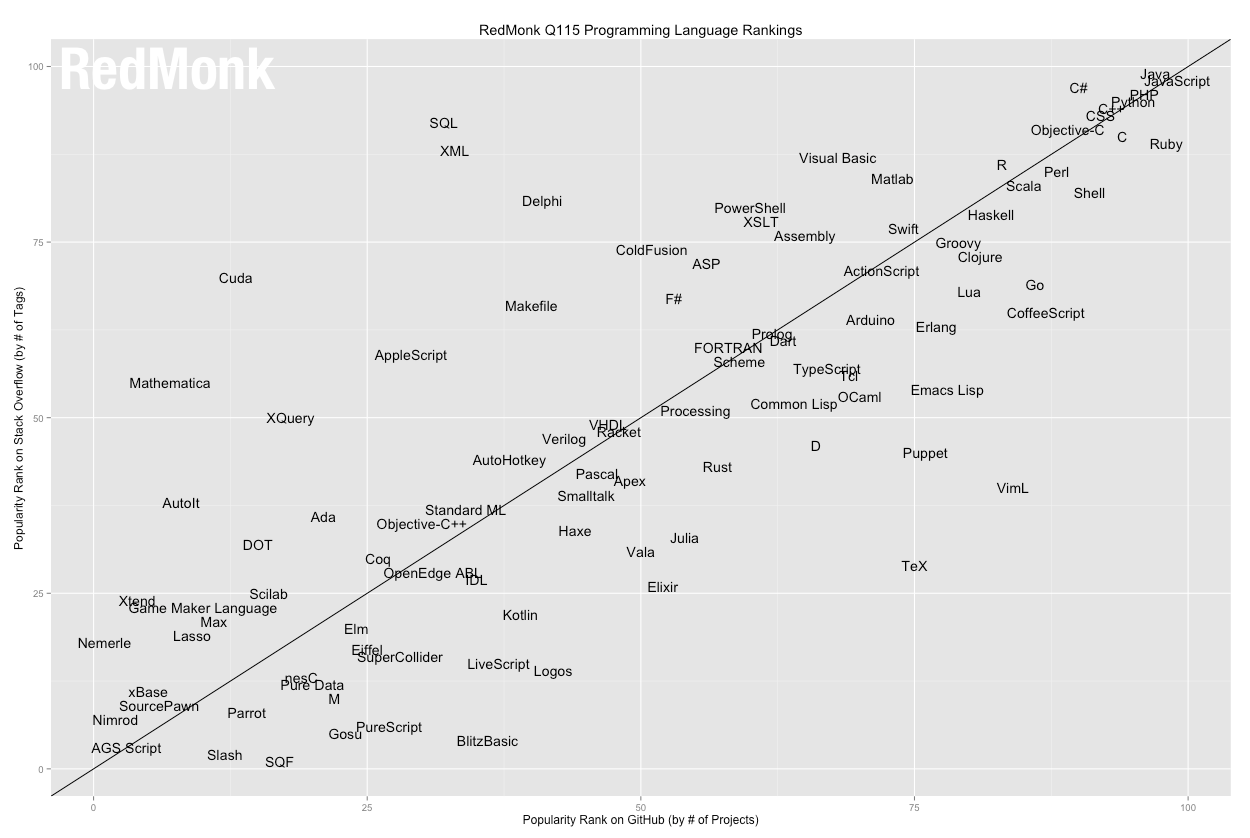
\includegraphics[width=1\textwidth]{img/grafico_redmonk}
	\caption{Ranking das liguagens de programação no Stack Overflow e Github}
\end{figure}


Ainda assim, para compor a interface do dado projeto, também ocorrerá o uso do líder JavaScript de forma intensa, provendo o elo com o as informações gerenciadas pelo PHP.


Entretanto, não seria inteligente desenvolver um sistema completo sem o auxílio de um framework. Dentre os frameworks disponíveis para PHP, hoje o destaque está com o Laravel, que se encontra no topo dentre os mais utilizados no momento. 


A WebHostFace, uma empresa de hospedagem, compilou várias estatísticas para criar um infográfico mostrando os frameworks PHP mais populares de 2015. Utilizando informações sobre os próprios clientes, o Google Trends, estatísticas de repositórios do GitHub e a pesquisa do SitePoint “Best PHP Frameworks 2015”, a WebHostFace elaborou o seguinte infográfico: 

\begin{figure}
	\label{fig:graficoWebhostface}
	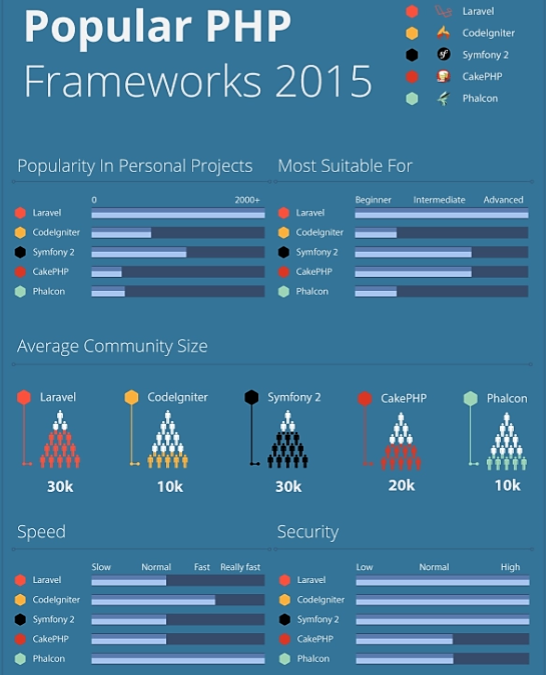
\includegraphics[width=1\textwidth]{img/infografico_webhostface}
	\caption{Infográfico da WebhostFace, exibindo a popularidade dos Frameworks PHP em 2015}
\end{figure}

Assim, tem-se a evidência que o Laravel em 2015 teve a maior popularidade em projetos pessoais e tem a maior comunidade entre os concorrentes, o que o torna uma boa escolha para a escrita de um software que será continuado por terceiros.


Para elaborar os recursos de interface e integrar ao back-end PHP do sistema, será adotado o já conhecido AngularJS, ferramenta sólida e conhecida no aspecto em questão. 


Dados coletados via Google Trends, que propõe comparações entre termos pesquisados, revela a popularidade do AngularJs diante de alguns dos principais concorrentes. O gráfico abaixo evidencia o cenário.


%Como mostra a Figura \ref{fig:graficoGoogleTrendsFerramentasFront}. 
\begin{figure}
	\label{fig:graficoGoogleTrendsFerramentasFront}
	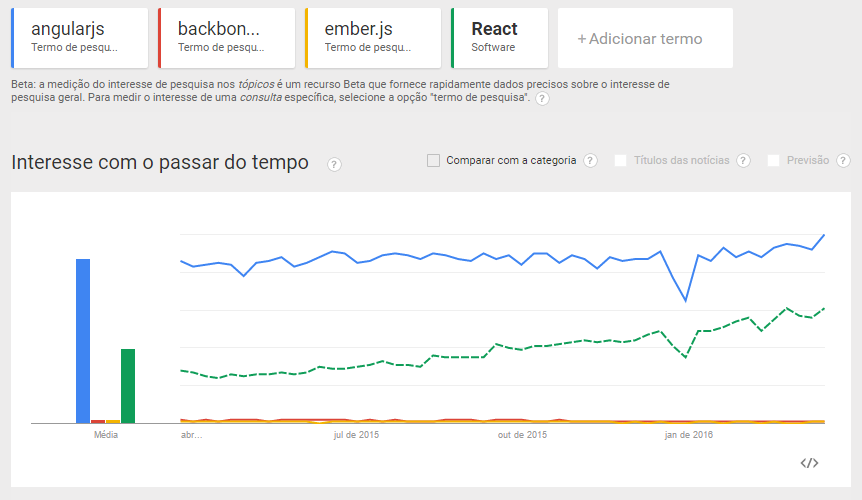
\includegraphics[width=1\textwidth]{img/grafico_ferramentas_front}
	\caption{Gráfico do Google Trends exibindo as pesquisas por ferramentas front-end}
\end{figure}


Junto ao Angular JS, será utilizada a agradável tendência de interface do Material Design da Google, que propõe layouts limpos e otimizados já conhecidos pelos usuários de smartphones Android. 


Para a elaboração da plataforma mobile do projeto, será utilizado o Ionic Framework, muito difundido e bastante pesquisado na área, o que fica evidenciado com o gráfico de pesquisbaixo, coletado via Google Trends buscando por frameworks de desenvolvimento híbrido mobile.


\begin{figure}
	\label{fig:graficoGoogleTrendsFerramentasHibridasMobile}
	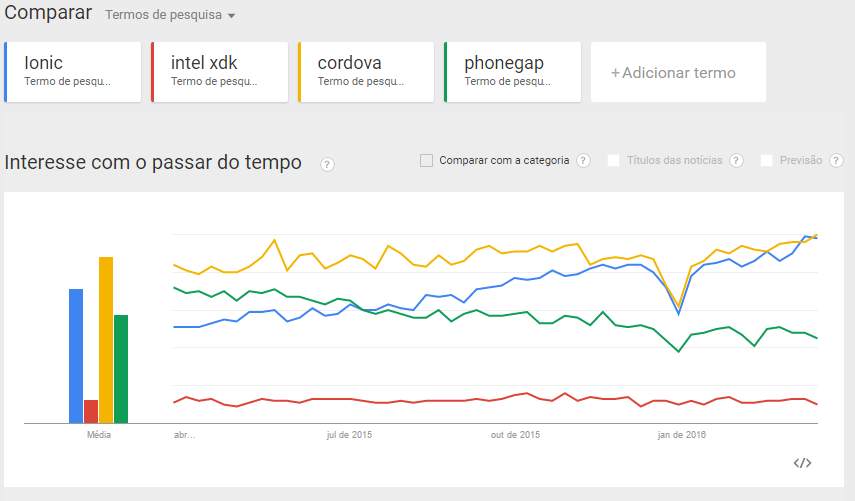
\includegraphics[width=1\textwidth]{img/grafico_ferramentas_hibridas_mobile}
	\caption{Gráfico do Google Trends exibindo as pesquisas por Frameworks híbridos mobile}
\end{figure}	

Para layout da interface mobile, também será aplicado a tendência do Material Design, a fim de propor uma harmonia entre o módulo web e mobile para os usuários


\section{Resultados Esperados}


Como fruto de um sistema para pós-graduação da UFBA, espera-se que os professores tenham mais recursos para integrar as atividades e também prover melhores condições para acompanhamento da vida acadêmica dos alunos em questão. Também, que os novos colaboradores que entrarem no processo tenham facilidade de compreender o fluxo do setor ao navegar pelo sistema proposto.


\section{Fora de Escopo}


Interação com os alunos devido às complicações para realizar a integração com o sistema empregado na UFBA, gerenciado pela XXXXXX, o que causaria uma inviabilidade no projeto devido à necessidade de entrega do produto ser mais forte que o tempo necessário para executar o processo de obtenção de acesso ao sistema legado para realizar a integração.


\section{Estrutura do Trabalho}


<breve resumo sobre os capítulos do TCC>
\chapter{Referencial Teórico}


Projetar o desenvolvimento de um software requer muito planejamento, pois as falhas iniciais podem custar bastante caro ou até mesmo inviabilizar a continuação de um projeto. Assim, a escolha da arquitetura ideal para a aplicabilidade é essencial na concepção de um produto de software. 
De todo o modo, sempre busca-se fazer mais com menos. Diante de tal filosofia, temos nesta seção, uma breve discussão sobre alguns elementos de projeto e arquitetura de software, a fim de contextualizar este trabalho de conclusão de curso.


% Ser direto no começo, focando no que realmente será discutido A seção \ref{sec:apps_mobile} 
 \section{Software como serviço}\label{sec:saas}


A definição de SaaS encontra-se muito bem elaborada em um dos trabalhos listados na literatura. Segundo La e Chun \citep{La2009Systematic}, o princípio da definição de Software como um Serviço (Sofware as a Service - SaaS) é um serviço complementar para aplicações da computação em nuvem (cloud computing). As duas áreas estão interligadas, no entanto, não se confundem, pois o SaaS deve ser entendido como um mecanismo de suporte às soluções existentes na cloud. Os SaaS existem justamente para maximizar o reuso de serviços repetidos e não centrais em uma aplicação remota.


Como propõe vantagens, software como servico é uma tendência forte, isso graças à evolução da web. Diversos fatores podem ser favoráveis para a adoção de um SaaS, como custo e manutenção dentre outros fatores aplicaveis a determinados contextos. Um trabalho recente realizado por Lechessa et al. \cite{LechesaSS11} apresenta uma pesquisa qualitativa sobre os fatores determinantes para adoção ou não de um SaaS voltado para ERP na África do Sul. Esses autores indicam que os principais fatores determinantes para adoção desse mecanismo de software são sua fluidez quanto à rede e a segurança. Esses fatores estão presentes na aplicação desenvolvida neste trabalho de conclusão de curso.
 

Devido ao fato de ter um serviço constantemente na nuvem, fica o questionamento sobre a segurança da informação manipulada. Sabe-se que a vulnerabilidade na web não é restrita ao SaaS, atingindo diversos âmbitos. O artigo de Rai et al. \cite{journals/corr/RaiSM13} orienta como o avanço da computação em nuvem não é um problema apenas para os serviços web do ponto de vista da segurança, pois muitos trabalhos na literatura mostram a área como mais um ponto de vulnerabilidade para diversos setores, a exemplo de infraestrutura. No mesmo artigo mencionado de Rai et al. \cite{journals/corr/RaiSM13}, também realizaram-se estudos exploratórios junto a empresas usuárias de serviços em computação em nuvem e consideram que a perspectiva de SaaS também pode fortalecer a segurança nas aplicações de cloud computing, pois o software de autenticação compartilhado por várias aplicações em nuvem, oferece uma melhor padronização e consequente facilidade de prevenção a erros de vulnerabilidade específicas de cada módulo da pesquisa. Esse ponto de vista é muito importante para qualquer trabalho de ponta na área de SaaS.


A arquitetura de armazenamento de dados de um Saas pode variar de acordo com a necessidade do contexto. O artigo recente de Huixin \cite{7586486}, exemplifica possíveis modelagens para utilizar. Tal abordagem pode ser com um banco de dados único, fazendo com que diferentes clientes compartilhem o mesmo banco, diferindo os dados através de controle de usuário, ou isolando os diferentes clientes através de bancos de dados exclusivos para cada um. Tal fator também pode ser combinado com a arquitetura da aplicação, caso ofereça aplicação única para todos os clientes ou aplicação compartilhada. Diante das possíveis abprdagens, a modelagem de dados do software pode ser decidida pela regra de negócio. Este trabalho optou por aplicação única e banco de dados compartilhado.


Devido ao diferente conceito de obtenção de software, tanto pela visão do cliente como pela visão do vendedor, é necessário tomar conhecimento dos diversos fatores que podem ser relevantes ao orçar um Saas. O recente trabalho de T. Kaur et al. \citep{6949281} orienta um modelo para compor o custo de um Saas. O custo total seria composto pelos fatores que dão suporte ao funcionamento do software. Tais fatores incluem infra-estrutura, configurabilidade, customização, parâmetros de QoS(Quality of service) como escalabilidade, disponibilidade, usabilidade, pontualidade e desempenho da resposta, portabilidade, custo total de propriedade e retorno do investimento. Esses fatores caracterizam o custo de forma eficaz, possibilitando ao fornecedor, prover um Serviço de acordo com a exigência do consumidor em vários pacotes de serviços.


\section{Reuso de software}\label{sec:reuso} %CRUISE BOOK CAPITULO 2


Para Peter Freeman, o reuso é a utilização de qualquer informação que um desenvolvedor pode necessitar no processo de criação de software (Ezran et al., 2002). Basili e Rombach definem reutilização de software como o uso de tudo o que está associado a um projeto de conhecimento (Basili e Rombach, 1991).
Assim, o objetivo da reutilização de software é reciclar o design, código e outros componentes de um produto de software e assim reduzir o custo, o tempo e melhorar a qualidade do produto.
Segundo Keswani et al. \cite{6783445}, o componente reutilizável de software pode ser qualquer parte de seu desenvolvimento, como um fragmento de código, design, casos de teste, ou até mesmo a especificação de requisitos de uma funcionalidade do software. 

O reuso de software pode ter impacto positivo em diversos aspectos do software, vejamos alguns, conforme apresentados no C.R.U.I.S.E Book:

\begin{itemize}

\item Qualidade: As correções de erro tornam-se úteis em todos os locais em que ocorreu, padronizando e facilitando a manutenção.

\item Produtividade: O ganho de produtividade é alcançado devido ao menor número de artefatos desenvolvido. Isso resulta em menos esforços de teste e também economiza análise e design, gerando economia em diversos escopos do projeto.

\item Confiabilidade: A utilização de componentes bem testados aumenta a
confiança no software. Além disso, a utilização de um mesmo componente em vários sistemas, aumenta a possibilidade de detecção de erros e reforça a confiança no componente.

\item Redução do Esforço: A reutilização de software proporciona uma redução do tempo de desenvolvimento, o que reduz o tempo necessário para o produto ser disponibilizado no mercado para trazer rentabilidade.

\item Trabalho redundante e tempo de desenvolvimento: Desenvolver um sistema do
zero significa desenvolvimento redundante de muitos componentes, como requisito
especificações, casos de uso, arquitetura, etc. Isso pode ser evitado quando estes estão disponíveis como componentes reutilizáveis e podem ser compartilhados, resultando em menos desenvolvimento, tempo e custo associado.

\item Documentação: Embora a documentação seja muito importante para a
manutenção de um sistema, muitas vezes é negligenciada. A reutilização de componentes software reduz a quantidade de documentação a ser escrita, entretanto depende da qualidade do que está escrito. Assim, apenas a estrutura do sistema e os novos artefatos desenvolvidos necessitam ser documentados.

\item Custo de manutenção: Menos defeitos e manutenções são esperados quando tem-se comprovada a qualidade dos componentes utilizados.

\item Tamanho da equipe: É comum entrar casos em que a equipe de desenvolvimento sofre sobrecarga. Entretanto, dobrar o tamanho da equipe de desenvolvimento não necessariamente duplica produtividade. Se muitos componentes podem ser reutilizados, é possível desenvolver com equipes menores, levando a melhores comunicações e aumento da produtividade.

\end{itemize}

Apesar dos benefícios da reutilização de software, a mesma não é amplamente praticado como imagina-se. Existem fatores que influenciam direta ou indiretamente na sua adoção. Esses fatores podem ser de aspecto gerencial, organizacional, econômico, conceitual ou técnico. Veremos a seguir alguns aspectos que podem gerar conflito com a cultura de reuso de software, segundo o C.R.U.I.S.E Book:
%(Sametinger, 1997). REVER

\begin{itemize}
	
\item Falta de apoio da gestão: Como a reutilização de software gera custos iniciais,
a medida pode não ser amplamente alcançada em uma organização sem o apoio de alto nível gestão. Os gestores têm de ser informados sobre os custos iniciais e serem convencidos sobre economias futuras.

\item Gerenciamento do Projeto: Gerenciar projetos tradicionais é uma tarefa árdua, principalmente, os que praticam a reutilização de software. Utilizando a técnica em larga escala, tem-se impacto sobre todo o ciclo de vida do software.

\item Estruturas organizacionais inadequadas: As estruturas organizacionais devem
considerar diferentes necessidades que surgem quando a reutilização em larga escala está sendo adotada. Por exemplo, uma equipe particionada pode ser alocada somente para desenvolver, manter e certificar componentes reutilizáveis de software.

\item Incentivos de gestão: É comum a falta de incentivo para deixar os desenvolvedores gastarem tempo elaborando reutilizáveis componentes do sistema. A produtividade é muitas vezes medida apenas no tempo necessário para concluir um projeto. Assim, fazer qualquer trabalho além disso, embora benéfico para a empresa como um todo, diminui o seu sucesso. Mesmo quando os componentes reutilizáveis são utilizados, os benefícios obtidos são uma pequena fração do que poderia ser alcançado caso houvesse reutilização explícita, planejada e organizada.

\item Dificuldade de encontrar software reutilizável: Para reutilizar os componentes, devem existir formas eficientes de busca. Além disso, é importante ter um repositório bem organizado contendo componentes com um eficiente meio de acesso.

\item Não reutilização do software encontrado. O acesso fácil ao software existente
não necessariamente aumentar a reutilização. Os componentes reutilizáveis devem ser cuidadosamente especificados, projetados, implementados e documentados, pois em alguns casos, modificar e adaptar o código  pode ser mais custoso que a programação da funcionalidade necessária a partir do zero.

\item Modificação: É muito difícil encontrar um componente que funcione
exatamente da mesma maneira que queremos. Desta forma, são necessárias modificações e devem existir formas de determinar os seus efeitos sobre o componente.


\end{itemize}


%Outra diretriz importante para a reutilização de software é reduzir o risco na criação de novos softwares. O risco tende a ser bastante reduzido se os componentes que estão sendo reutilizados têm as documentação, interfaces necessárias e devidamente testadas, fatores que contibruem para uma fácil integração.
%De acordo com Keswani et al. \citep{6783445}, para o reuso de software dar retornos apropriados, o processo deve ser sistemático e planejado. Qualquer organização que implemente a reutilização de software deve identificar os melhores métodos e estratégias de reutilização para obter a máxima produtividade. A reutilização de software ajuda a evitar software de engenharia a partir do zero, pois usa módulos de software existentes. A reutilização de software, embora seja uma tarefa difícil, especialmente para softwares antigos sem padrões de projeto, pode melhorar significativamente a produtividade e a qualidade de um produto de software. Embora a reutilização de software não seja um novo campo, ela pode dar grandes retornos em curto período de tempo.


\section{Modularização}\label{sec:modularizacao} %artigo de claudio pagina 222 introdução


%A modularidade vem desempenhando um papel predominante estágios emergentes das disciplinas de arquitetura de software [13]. Engenheiros de software consideram modularidade como princípio base na comparação entre arquiteturas alternativas  e arquitetura degeneração [9]. De fato, os engenheiros de software são incentivados a arquitecturas, baseando-se numa multiplicidade de mecanismos de modularidade disponíveis em: 
%(i) Linguagens de descrição de arquitetura (ADLs), como ACME [8], 
%(ii) catálogos de arquitetônicos [2, 13], e 
%(iii) conhecem bem princípios de alto nível, como interfaces de componentes estreitos, acoplamento arquitectónico reduzido e semelhantes.


Conforme é frisado no trabalho de Wickramaarachchi e Lai \citep{7062705}, o conceito de modularização na indústria de software tem uma longa história e tem sido utilizado para melhorar o processo de desenvolvimento de software em diferentes estágios. Os principais conceitos por trás da modularização do software foram introduzidos por pesquisadores pioneiros há quarenta anos, com uma notável contribuição feita por Melvin Conway e David Parnas, que tem representação notável na engenharia de software.


Modularizar um software é um bom padrão a ser adotado. Segundo Wickramaarachchi e Lai \citep{7062705}, a modularização é importante na identificação de dependências e reduz as dificuldades diante de uma possível necessidade de grandes alterações. De uma perspectiva da engenharia de software, uma modularização geralmente tem várias vantagens, tais como: tornar a complexidade do software mais gerenciável, facilitar o trabalho paralelo e tornar o software mais maleável para acomodar o futuro incerto que um software pode ter. O objetivo final da modularização do software é aumentar a produtividade ea qualidade do software. Tal conceito encontra-se bastante difundido e estái incorporado em linguagens de programação e ferramentas de software. O trabalho proposto favorece ao uso da modularização de um software e até mesmo pode ser considerado um módulo a ser acoplado a qualquer software, mediante a compatibilidade.


\section{Aplicações web}\label{sec:apps_web}


A popularidade da aplicação web aumentou exponencialmente na última década e todos os dias cresce o número de pessoas usuárias de aplicações web. E seguindo o padrão de desenvolvimento de software, Kumar et al. \citep{7813710} sugerem que para o desenvolvimento web, deve-se manter a prática efiacaz de produzir diagramas UML. A abordagem baseada na web oferece uma maneira fácil e eficaz para gerenciar e controlar o processo de desenvolvimento por meio de diagramas UML. Tal abordagem pode ser usada quando há uma exigência de lidar com mudanças muito rápidas e grandes em requisitos de forma muito eficaz em muito menos tempo, gerando assim um menor impacto. 


Para atender à fomentada demanda de aplicativos web, é necessário adotar métodos de desenvolvimentos que sejam ágeis, eficientes e de fácil manutenção. Yu Ping et al. \cite{1372143} propõem o uso do modelo MVC (Model, View e Controller) no atual desenvolvimento para softwares web. O modelo apresentado tornou-se um padrão popular e divide o software em camadas com propósito definido, tornando-o de mais fácil manutenção.


O Ajax (Asynchronous Javascript and XML) revolucionou a web. Conforme demonstrado no artigo de Yuping \citep{6845605}, ao usar a tecnologia Ajax, podemos enriquecer a experiência do usuário em aplicações baseadas em navegador de internet, e fornecer uma variedade de aplicações interativas para atender às necessidade de humanização das aplicações.
Os aplicativos Ajax em execução no navegador se comunicam com um servidor Web de forma assíncrona e atualizam apenas uma parte da página.



% %% RiSE Latex Template - version 0.5
%%
%% RiSE's latex template for thesis and dissertations
%% http://risetemplate.sourceforge.net
%%
%% (c) 2012 Yguaratã Cerqueira Cavalcanti (yguarata@gmail.com)
%%          Vinicius Cardoso Garcia (vinicius.garcia@gmail.com)
%%
%% This document was initially based on UFPEThesis template, from Paulo Gustavo
%% S. Fonseca.
%%
%% ACKNOWLEDGEMENTS
%%
%% We would like to thanks the RiSE's researchers community, the 
%% students from Federal University of Pernambuco, and other users that have
%% been contributing to this projects with comments and patches.
%%
%% GENERAL INSTRUCTIONS
%%
%% We strongly recommend you to compile your documents using pdflatex command.
%% It is also recommend use the texlipse plugin for Eclipse to edit your documents.
%%
%% Options for \documentclass command:
%%         * Idiom
%%           pt   - Portguese (default)
%%           en   - English
%%
%%         * Text type
%%           bsc  - B.Sc. Thesis
%%           msc  - M.Sc. Thesis (default)
%%           qual - PHD qualification (not tested yet)
%%           prop - PHD proposal (not tested yet)
%%           phd  - PHD thesis
%%
%%         * Media
%%           scr  - to eletronic version (PDF) / see the users guide
%%
%%         * Pagination
%%           oneside - unique face press
%%           twoside - two faces press
%%
%%		   * Line spacing
%%           singlespacing  - the same as using \linespread{1}
%%           onehalfspacing - the same as using \linespread{1.3}
%%           doublespacing  - the same as using \linespread{1.6}
%%
%% Reference commands. Use the following commands to make references in your
%% text:
%%          \figref  -- for Figure reference
%%          \tabref  -- for Table reference
%%          \eqnref  -- for equation reference
%%          \chapref -- for chapter reference
%%          \secref  -- for section reference
%%          \appref  -- for appendix reference
%%          \axiref  -- for axiom reference
%%          \conjref -- for conjecture reference
%%          \defref  -- for definition reference
%%          \lemref  -- for lemma reference
%%          \theoref -- for theorem reference
%%          \corref  -- for corollary reference
%%          \propref -- for proprosition reference
%%          \pgref   -- for page reference
%%
%%          Example: See \chapref{chap:introduction}. It will produce 
%%                   'See Chapter 1', in case of English language.

\documentclass[pt,twoside,onehalfspacing,bsc]{risethesis}

\usepackage[utf8]{inputenc}
\usepackage[brazilian]{babel}
\usepackage[T1]{fontenc}

%% Change the following pdf author attribute name to your name.
\usepackage[linkcolor=blue,citecolor=blue,urlcolor=blue,colorlinks,pdfpagelabels,pdftitle={Bruno Cabral's Bachelor Thesis},pdfauthor={Bruno Cabral}]{hyperref}

\address{SALVADOR}

\universitypt{Universidade Federal da Bahia}
\universityen{Federal University of Bahia}

\departmentpt{Depertamento de Ciência da Computação}
\departmenten{Computer Science Department}

\programpt{Programa Multiinstitucional de Pós-graduação em Ciência da Computação}
\programen{Graduate in Computer Science}

\majorfieldpt{Ciência da Computação}
\majorfielden{Computer Science}

\title{Sistema de apoio à Pós graduação - UFBA}
\date{Outubro/2016}

\author{Victor de Azevedo Nunes}
\adviser{Ivan do Carmo Machado}

\begin{document}

\frontmatter
\frontpage
\presentationpage

\begin{dedicatory}
Eu dedico esta dissertação...
%I dedicate this dissertation to my family, girlfriend, friends and
%professors who gave me all necessary support to get here.
\end{dedicatory}

\acknowledgements
Meus agradecimentos...

\begin{epigraph}[]{Edward V Berard}
Walking on water and developing software from a specification are easy if both are frozen
\end{epigraph}

\resumo
% Escreva seu resumo no arquivo resumo.tex
\input{resumo}

\abstract
% Write your abstract in a file called abstract.tex
\input{abstract}

% Summary (tables of contents)
\tableofcontents

% List of figures
\listoffigures

% List of tables
\listoftables

% List of acronyms
% Acronyms manual: http://linorg.usp.br/CTAN/macros/latex/contrib/acronym/acronym.pdf
\listofacronyms
\input{acronyms}

% List of listings
%\lstlistoflistings

\mainmatter

\include{chapters/intro}
\include{chapters/referencial_teorico}

% \include{chapters/introduction/main}
% \include{chapters/background/main}
% \include{chapters/proposed_solution/main}
% \include{chapters/experiment/main}
% \include{chapters/conclusion/main}

\bibliographystyle{natbib}
\addcontentsline{toc}{chapter}{\bibliographytocname}
\bibliography{references}

% Appendix
\clearpage
\addappheadtotoc
\appendix
\appendixpage
% \include{appendix/experiment-instruments}

\end{document}
% %% RiSE Latex Template - version 0.5
%%
%% RiSE's latex template for thesis and dissertations
%% http://risetemplate.sourceforge.net
%%
%% (c) 2012 Yguaratã Cerqueira Cavalcanti (yguarata@gmail.com)
%%          Vinicius Cardoso Garcia (vinicius.garcia@gmail.com)
%%
%% This document was initially based on UFPEThesis template, from Paulo Gustavo
%% S. Fonseca.
%%
%% ACKNOWLEDGEMENTS
%%
%% We would like to thanks the RiSE's researchers community, the 
%% students from Federal University of Pernambuco, and other users that have
%% been contributing to this projects with comments and patches.
%%
%% GENERAL INSTRUCTIONS
%%
%% We strongly recommend you to compile your documents using pdflatex command.
%% It is also recommend use the texlipse plugin for Eclipse to edit your documents.
%%
%% Options for \documentclass command:
%%         * Idiom
%%           pt   - Portguese (default)
%%           en   - English
%%
%%         * Text type
%%           bsc  - B.Sc. Thesis
%%           msc  - M.Sc. Thesis (default)
%%           qual - PHD qualification (not tested yet)
%%           prop - PHD proposal (not tested yet)
%%           phd  - PHD thesis
%%
%%         * Media
%%           scr  - to eletronic version (PDF) / see the users guide
%%
%%         * Pagination
%%           oneside - unique face press
%%           twoside - two faces press
%%
%%		   * Line spacing
%%           singlespacing  - the same as using \linespread{1}
%%           onehalfspacing - the same as using \linespread{1.3}
%%           doublespacing  - the same as using \linespread{1.6}
%%
%% Reference commands. Use the following commands to make references in your
%% text:
%%          \figref  -- for Figure reference
%%          \tabref  -- for Table reference
%%          \eqnref  -- for equation reference
%%          \chapref -- for chapter reference
%%          \secref  -- for section reference
%%          \appref  -- for appendix reference
%%          \axiref  -- for axiom reference
%%          \conjref -- for conjecture reference
%%          \defref  -- for definition reference
%%          \lemref  -- for lemma reference
%%          \theoref -- for theorem reference
%%          \corref  -- for corollary reference
%%          \propref -- for proprosition reference
%%          \pgref   -- for page reference
%%
%%          Example: See \chapref{chap:introduction}. It will produce 
%%                   'See Chapter 1', in case of English language.

\documentclass[pt,twoside,onehalfspacing,bsc]{risethesis}

\usepackage[utf8]{inputenc}
\usepackage[brazilian]{babel}
\usepackage[T1]{fontenc}

%% Change the following pdf author attribute name to your name.
\usepackage[linkcolor=blue,citecolor=blue,urlcolor=blue,colorlinks,pdfpagelabels,pdftitle={Bruno Cabral's Bachelor Thesis},pdfauthor={Bruno Cabral}]{hyperref}

\address{SALVADOR}

\universitypt{Universidade Federal da Bahia}
\universityen{Federal University of Bahia}

\departmentpt{Depertamento de Ciência da Computação}
\departmenten{Computer Science Department}

\programpt{Programa Multiinstitucional de Pós-graduação em Ciência da Computação}
\programen{Graduate in Computer Science}

\majorfieldpt{Ciência da Computação}
\majorfielden{Computer Science}

\title{Sistema de apoio à Pós graduação - UFBA}
\date{Outubro/2016}

\author{Victor de Azevedo Nunes}
\adviser{Ivan do Carmo Machado}

\begin{document}

\frontmatter
\frontpage
\presentationpage

\begin{dedicatory}
Eu dedico esta dissertação...
%I dedicate this dissertation to my family, girlfriend, friends and
%professors who gave me all necessary support to get here.
\end{dedicatory}

\acknowledgements
Meus agradecimentos...

\begin{epigraph}[]{Edward V Berard}
Walking on water and developing software from a specification are easy if both are frozen
\end{epigraph}

\resumo
% Escreva seu resumo no arquivo resumo.tex
\input{resumo}

\abstract
% Write your abstract in a file called abstract.tex
\input{abstract}

% Summary (tables of contents)
\tableofcontents

% List of figures
\listoffigures

% List of tables
\listoftables

% List of acronyms
% Acronyms manual: http://linorg.usp.br/CTAN/macros/latex/contrib/acronym/acronym.pdf
\listofacronyms
\input{acronyms}

% List of listings
%\lstlistoflistings

\mainmatter

\include{chapters/intro}
\include{chapters/referencial_teorico}

% \include{chapters/introduction/main}
% \include{chapters/background/main}
% \include{chapters/proposed_solution/main}
% \include{chapters/experiment/main}
% \include{chapters/conclusion/main}

\bibliographystyle{natbib}
\addcontentsline{toc}{chapter}{\bibliographytocname}
\bibliography{references}

% Appendix
\clearpage
\addappheadtotoc
\appendix
\appendixpage
% \include{appendix/experiment-instruments}

\end{document}
% %% RiSE Latex Template - version 0.5
%%
%% RiSE's latex template for thesis and dissertations
%% http://risetemplate.sourceforge.net
%%
%% (c) 2012 Yguaratã Cerqueira Cavalcanti (yguarata@gmail.com)
%%          Vinicius Cardoso Garcia (vinicius.garcia@gmail.com)
%%
%% This document was initially based on UFPEThesis template, from Paulo Gustavo
%% S. Fonseca.
%%
%% ACKNOWLEDGEMENTS
%%
%% We would like to thanks the RiSE's researchers community, the 
%% students from Federal University of Pernambuco, and other users that have
%% been contributing to this projects with comments and patches.
%%
%% GENERAL INSTRUCTIONS
%%
%% We strongly recommend you to compile your documents using pdflatex command.
%% It is also recommend use the texlipse plugin for Eclipse to edit your documents.
%%
%% Options for \documentclass command:
%%         * Idiom
%%           pt   - Portguese (default)
%%           en   - English
%%
%%         * Text type
%%           bsc  - B.Sc. Thesis
%%           msc  - M.Sc. Thesis (default)
%%           qual - PHD qualification (not tested yet)
%%           prop - PHD proposal (not tested yet)
%%           phd  - PHD thesis
%%
%%         * Media
%%           scr  - to eletronic version (PDF) / see the users guide
%%
%%         * Pagination
%%           oneside - unique face press
%%           twoside - two faces press
%%
%%		   * Line spacing
%%           singlespacing  - the same as using \linespread{1}
%%           onehalfspacing - the same as using \linespread{1.3}
%%           doublespacing  - the same as using \linespread{1.6}
%%
%% Reference commands. Use the following commands to make references in your
%% text:
%%          \figref  -- for Figure reference
%%          \tabref  -- for Table reference
%%          \eqnref  -- for equation reference
%%          \chapref -- for chapter reference
%%          \secref  -- for section reference
%%          \appref  -- for appendix reference
%%          \axiref  -- for axiom reference
%%          \conjref -- for conjecture reference
%%          \defref  -- for definition reference
%%          \lemref  -- for lemma reference
%%          \theoref -- for theorem reference
%%          \corref  -- for corollary reference
%%          \propref -- for proprosition reference
%%          \pgref   -- for page reference
%%
%%          Example: See \chapref{chap:introduction}. It will produce 
%%                   'See Chapter 1', in case of English language.

\documentclass[pt,twoside,onehalfspacing,bsc]{risethesis}

\usepackage[utf8]{inputenc}
\usepackage[brazilian]{babel}
\usepackage[T1]{fontenc}

%% Change the following pdf author attribute name to your name.
\usepackage[linkcolor=blue,citecolor=blue,urlcolor=blue,colorlinks,pdfpagelabels,pdftitle={Bruno Cabral's Bachelor Thesis},pdfauthor={Bruno Cabral}]{hyperref}

\address{SALVADOR}

\universitypt{Universidade Federal da Bahia}
\universityen{Federal University of Bahia}

\departmentpt{Depertamento de Ciência da Computação}
\departmenten{Computer Science Department}

\programpt{Programa Multiinstitucional de Pós-graduação em Ciência da Computação}
\programen{Graduate in Computer Science}

\majorfieldpt{Ciência da Computação}
\majorfielden{Computer Science}

\title{Sistema de apoio à Pós graduação - UFBA}
\date{Outubro/2016}

\author{Victor de Azevedo Nunes}
\adviser{Ivan do Carmo Machado}

\begin{document}

\frontmatter
\frontpage
\presentationpage

\begin{dedicatory}
Eu dedico esta dissertação...
%I dedicate this dissertation to my family, girlfriend, friends and
%professors who gave me all necessary support to get here.
\end{dedicatory}

\acknowledgements
Meus agradecimentos...

\begin{epigraph}[]{Edward V Berard}
Walking on water and developing software from a specification are easy if both are frozen
\end{epigraph}

\resumo
% Escreva seu resumo no arquivo resumo.tex
\input{resumo}

\abstract
% Write your abstract in a file called abstract.tex
\input{abstract}

% Summary (tables of contents)
\tableofcontents

% List of figures
\listoffigures

% List of tables
\listoftables

% List of acronyms
% Acronyms manual: http://linorg.usp.br/CTAN/macros/latex/contrib/acronym/acronym.pdf
\listofacronyms
\input{acronyms}

% List of listings
%\lstlistoflistings

\mainmatter

\include{chapters/intro}
\include{chapters/referencial_teorico}

% \include{chapters/introduction/main}
% \include{chapters/background/main}
% \include{chapters/proposed_solution/main}
% \include{chapters/experiment/main}
% \include{chapters/conclusion/main}

\bibliographystyle{natbib}
\addcontentsline{toc}{chapter}{\bibliographytocname}
\bibliography{references}

% Appendix
\clearpage
\addappheadtotoc
\appendix
\appendixpage
% \include{appendix/experiment-instruments}

\end{document}
% %% RiSE Latex Template - version 0.5
%%
%% RiSE's latex template for thesis and dissertations
%% http://risetemplate.sourceforge.net
%%
%% (c) 2012 Yguaratã Cerqueira Cavalcanti (yguarata@gmail.com)
%%          Vinicius Cardoso Garcia (vinicius.garcia@gmail.com)
%%
%% This document was initially based on UFPEThesis template, from Paulo Gustavo
%% S. Fonseca.
%%
%% ACKNOWLEDGEMENTS
%%
%% We would like to thanks the RiSE's researchers community, the 
%% students from Federal University of Pernambuco, and other users that have
%% been contributing to this projects with comments and patches.
%%
%% GENERAL INSTRUCTIONS
%%
%% We strongly recommend you to compile your documents using pdflatex command.
%% It is also recommend use the texlipse plugin for Eclipse to edit your documents.
%%
%% Options for \documentclass command:
%%         * Idiom
%%           pt   - Portguese (default)
%%           en   - English
%%
%%         * Text type
%%           bsc  - B.Sc. Thesis
%%           msc  - M.Sc. Thesis (default)
%%           qual - PHD qualification (not tested yet)
%%           prop - PHD proposal (not tested yet)
%%           phd  - PHD thesis
%%
%%         * Media
%%           scr  - to eletronic version (PDF) / see the users guide
%%
%%         * Pagination
%%           oneside - unique face press
%%           twoside - two faces press
%%
%%		   * Line spacing
%%           singlespacing  - the same as using \linespread{1}
%%           onehalfspacing - the same as using \linespread{1.3}
%%           doublespacing  - the same as using \linespread{1.6}
%%
%% Reference commands. Use the following commands to make references in your
%% text:
%%          \figref  -- for Figure reference
%%          \tabref  -- for Table reference
%%          \eqnref  -- for equation reference
%%          \chapref -- for chapter reference
%%          \secref  -- for section reference
%%          \appref  -- for appendix reference
%%          \axiref  -- for axiom reference
%%          \conjref -- for conjecture reference
%%          \defref  -- for definition reference
%%          \lemref  -- for lemma reference
%%          \theoref -- for theorem reference
%%          \corref  -- for corollary reference
%%          \propref -- for proprosition reference
%%          \pgref   -- for page reference
%%
%%          Example: See \chapref{chap:introduction}. It will produce 
%%                   'See Chapter 1', in case of English language.

\documentclass[pt,twoside,onehalfspacing,bsc]{risethesis}

\usepackage[utf8]{inputenc}
\usepackage[brazilian]{babel}
\usepackage[T1]{fontenc}

%% Change the following pdf author attribute name to your name.
\usepackage[linkcolor=blue,citecolor=blue,urlcolor=blue,colorlinks,pdfpagelabels,pdftitle={Bruno Cabral's Bachelor Thesis},pdfauthor={Bruno Cabral}]{hyperref}

\address{SALVADOR}

\universitypt{Universidade Federal da Bahia}
\universityen{Federal University of Bahia}

\departmentpt{Depertamento de Ciência da Computação}
\departmenten{Computer Science Department}

\programpt{Programa Multiinstitucional de Pós-graduação em Ciência da Computação}
\programen{Graduate in Computer Science}

\majorfieldpt{Ciência da Computação}
\majorfielden{Computer Science}

\title{Sistema de apoio à Pós graduação - UFBA}
\date{Outubro/2016}

\author{Victor de Azevedo Nunes}
\adviser{Ivan do Carmo Machado}

\begin{document}

\frontmatter
\frontpage
\presentationpage

\begin{dedicatory}
Eu dedico esta dissertação...
%I dedicate this dissertation to my family, girlfriend, friends and
%professors who gave me all necessary support to get here.
\end{dedicatory}

\acknowledgements
Meus agradecimentos...

\begin{epigraph}[]{Edward V Berard}
Walking on water and developing software from a specification are easy if both are frozen
\end{epigraph}

\resumo
% Escreva seu resumo no arquivo resumo.tex
\input{resumo}

\abstract
% Write your abstract in a file called abstract.tex
\input{abstract}

% Summary (tables of contents)
\tableofcontents

% List of figures
\listoffigures

% List of tables
\listoftables

% List of acronyms
% Acronyms manual: http://linorg.usp.br/CTAN/macros/latex/contrib/acronym/acronym.pdf
\listofacronyms
\input{acronyms}

% List of listings
%\lstlistoflistings

\mainmatter

\include{chapters/intro}
\include{chapters/referencial_teorico}

% \include{chapters/introduction/main}
% \include{chapters/background/main}
% \include{chapters/proposed_solution/main}
% \include{chapters/experiment/main}
% \include{chapters/conclusion/main}

\bibliographystyle{natbib}
\addcontentsline{toc}{chapter}{\bibliographytocname}
\bibliography{references}

% Appendix
\clearpage
\addappheadtotoc
\appendix
\appendixpage
% \include{appendix/experiment-instruments}

\end{document}
% %% RiSE Latex Template - version 0.5
%%
%% RiSE's latex template for thesis and dissertations
%% http://risetemplate.sourceforge.net
%%
%% (c) 2012 Yguaratã Cerqueira Cavalcanti (yguarata@gmail.com)
%%          Vinicius Cardoso Garcia (vinicius.garcia@gmail.com)
%%
%% This document was initially based on UFPEThesis template, from Paulo Gustavo
%% S. Fonseca.
%%
%% ACKNOWLEDGEMENTS
%%
%% We would like to thanks the RiSE's researchers community, the 
%% students from Federal University of Pernambuco, and other users that have
%% been contributing to this projects with comments and patches.
%%
%% GENERAL INSTRUCTIONS
%%
%% We strongly recommend you to compile your documents using pdflatex command.
%% It is also recommend use the texlipse plugin for Eclipse to edit your documents.
%%
%% Options for \documentclass command:
%%         * Idiom
%%           pt   - Portguese (default)
%%           en   - English
%%
%%         * Text type
%%           bsc  - B.Sc. Thesis
%%           msc  - M.Sc. Thesis (default)
%%           qual - PHD qualification (not tested yet)
%%           prop - PHD proposal (not tested yet)
%%           phd  - PHD thesis
%%
%%         * Media
%%           scr  - to eletronic version (PDF) / see the users guide
%%
%%         * Pagination
%%           oneside - unique face press
%%           twoside - two faces press
%%
%%		   * Line spacing
%%           singlespacing  - the same as using \linespread{1}
%%           onehalfspacing - the same as using \linespread{1.3}
%%           doublespacing  - the same as using \linespread{1.6}
%%
%% Reference commands. Use the following commands to make references in your
%% text:
%%          \figref  -- for Figure reference
%%          \tabref  -- for Table reference
%%          \eqnref  -- for equation reference
%%          \chapref -- for chapter reference
%%          \secref  -- for section reference
%%          \appref  -- for appendix reference
%%          \axiref  -- for axiom reference
%%          \conjref -- for conjecture reference
%%          \defref  -- for definition reference
%%          \lemref  -- for lemma reference
%%          \theoref -- for theorem reference
%%          \corref  -- for corollary reference
%%          \propref -- for proprosition reference
%%          \pgref   -- for page reference
%%
%%          Example: See \chapref{chap:introduction}. It will produce 
%%                   'See Chapter 1', in case of English language.

\documentclass[pt,twoside,onehalfspacing,bsc]{risethesis}

\usepackage[utf8]{inputenc}
\usepackage[brazilian]{babel}
\usepackage[T1]{fontenc}

%% Change the following pdf author attribute name to your name.
\usepackage[linkcolor=blue,citecolor=blue,urlcolor=blue,colorlinks,pdfpagelabels,pdftitle={Bruno Cabral's Bachelor Thesis},pdfauthor={Bruno Cabral}]{hyperref}

\address{SALVADOR}

\universitypt{Universidade Federal da Bahia}
\universityen{Federal University of Bahia}

\departmentpt{Depertamento de Ciência da Computação}
\departmenten{Computer Science Department}

\programpt{Programa Multiinstitucional de Pós-graduação em Ciência da Computação}
\programen{Graduate in Computer Science}

\majorfieldpt{Ciência da Computação}
\majorfielden{Computer Science}

\title{Sistema de apoio à Pós graduação - UFBA}
\date{Outubro/2016}

\author{Victor de Azevedo Nunes}
\adviser{Ivan do Carmo Machado}

\begin{document}

\frontmatter
\frontpage
\presentationpage

\begin{dedicatory}
Eu dedico esta dissertação...
%I dedicate this dissertation to my family, girlfriend, friends and
%professors who gave me all necessary support to get here.
\end{dedicatory}

\acknowledgements
Meus agradecimentos...

\begin{epigraph}[]{Edward V Berard}
Walking on water and developing software from a specification are easy if both are frozen
\end{epigraph}

\resumo
% Escreva seu resumo no arquivo resumo.tex
\input{resumo}

\abstract
% Write your abstract in a file called abstract.tex
\input{abstract}

% Summary (tables of contents)
\tableofcontents

% List of figures
\listoffigures

% List of tables
\listoftables

% List of acronyms
% Acronyms manual: http://linorg.usp.br/CTAN/macros/latex/contrib/acronym/acronym.pdf
\listofacronyms
\input{acronyms}

% List of listings
%\lstlistoflistings

\mainmatter

\include{chapters/intro}
\include{chapters/referencial_teorico}

% \include{chapters/introduction/main}
% \include{chapters/background/main}
% \include{chapters/proposed_solution/main}
% \include{chapters/experiment/main}
% \include{chapters/conclusion/main}

\bibliographystyle{natbib}
\addcontentsline{toc}{chapter}{\bibliographytocname}
\bibliography{references}

% Appendix
\clearpage
\addappheadtotoc
\appendix
\appendixpage
% \include{appendix/experiment-instruments}

\end{document}

\bibliographystyle{natbib}
\addcontentsline{toc}{chapter}{\bibliographytocname}
\bibliography{references}

% Appendix
\clearpage
\addappheadtotoc
\appendix
\appendixpage
% \include{appendix/experiment-instruments}

\end{document}

\bibliographystyle{natbib}
\addcontentsline{toc}{chapter}{\bibliographytocname}
\bibliography{references}

% Appendix
\clearpage
\addappheadtotoc
\appendix
\appendixpage
% \include{appendix/experiment-instruments}

\end{document}
% %% RiSE Latex Template - version 0.5
%%
%% RiSE's latex template for thesis and dissertations
%% http://risetemplate.sourceforge.net
%%
%% (c) 2012 Yguaratã Cerqueira Cavalcanti (yguarata@gmail.com)
%%          Vinicius Cardoso Garcia (vinicius.garcia@gmail.com)
%%
%% This document was initially based on UFPEThesis template, from Paulo Gustavo
%% S. Fonseca.
%%
%% ACKNOWLEDGEMENTS
%%
%% We would like to thanks the RiSE's researchers community, the 
%% students from Federal University of Pernambuco, and other users that have
%% been contributing to this projects with comments and patches.
%%
%% GENERAL INSTRUCTIONS
%%
%% We strongly recommend you to compile your documents using pdflatex command.
%% It is also recommend use the texlipse plugin for Eclipse to edit your documents.
%%
%% Options for \documentclass command:
%%         * Idiom
%%           pt   - Portguese (default)
%%           en   - English
%%
%%         * Text type
%%           bsc  - B.Sc. Thesis
%%           msc  - M.Sc. Thesis (default)
%%           qual - PHD qualification (not tested yet)
%%           prop - PHD proposal (not tested yet)
%%           phd  - PHD thesis
%%
%%         * Media
%%           scr  - to eletronic version (PDF) / see the users guide
%%
%%         * Pagination
%%           oneside - unique face press
%%           twoside - two faces press
%%
%%		   * Line spacing
%%           singlespacing  - the same as using \linespread{1}
%%           onehalfspacing - the same as using \linespread{1.3}
%%           doublespacing  - the same as using \linespread{1.6}
%%
%% Reference commands. Use the following commands to make references in your
%% text:
%%          \figref  -- for Figure reference
%%          \tabref  -- for Table reference
%%          \eqnref  -- for equation reference
%%          \chapref -- for chapter reference
%%          \secref  -- for section reference
%%          \appref  -- for appendix reference
%%          \axiref  -- for axiom reference
%%          \conjref -- for conjecture reference
%%          \defref  -- for definition reference
%%          \lemref  -- for lemma reference
%%          \theoref -- for theorem reference
%%          \corref  -- for corollary reference
%%          \propref -- for proprosition reference
%%          \pgref   -- for page reference
%%
%%          Example: See \chapref{chap:introduction}. It will produce 
%%                   'See Chapter 1', in case of English language.

\documentclass[pt,twoside,onehalfspacing,bsc]{risethesis}

\usepackage[utf8]{inputenc}
\usepackage[brazilian]{babel}
\usepackage[T1]{fontenc}

%% Change the following pdf author attribute name to your name.
\usepackage[linkcolor=blue,citecolor=blue,urlcolor=blue,colorlinks,pdfpagelabels,pdftitle={Bruno Cabral's Bachelor Thesis},pdfauthor={Bruno Cabral}]{hyperref}

\address{SALVADOR}

\universitypt{Universidade Federal da Bahia}
\universityen{Federal University of Bahia}

\departmentpt{Depertamento de Ciência da Computação}
\departmenten{Computer Science Department}

\programpt{Programa Multiinstitucional de Pós-graduação em Ciência da Computação}
\programen{Graduate in Computer Science}

\majorfieldpt{Ciência da Computação}
\majorfielden{Computer Science}

\title{Sistema de apoio à Pós graduação - UFBA}
\date{Outubro/2016}

\author{Victor de Azevedo Nunes}
\adviser{Ivan do Carmo Machado}

\begin{document}

\frontmatter
\frontpage
\presentationpage

\begin{dedicatory}
Eu dedico esta dissertação...
%I dedicate this dissertation to my family, girlfriend, friends and
%professors who gave me all necessary support to get here.
\end{dedicatory}

\acknowledgements
Meus agradecimentos...

\begin{epigraph}[]{Edward V Berard}
Walking on water and developing software from a specification are easy if both are frozen
\end{epigraph}

\resumo
% Escreva seu resumo no arquivo resumo.tex
Meu resumo

\begin{keywords}
palavras chave

\end{keywords}

\abstract
% Write your abstract in a file called abstract.tex
My abstract...

\begin{keywords}
key words...
\end{keywords}

% Summary (tables of contents)
\tableofcontents

% List of figures
\listoffigures

% List of tables
\listoftables

% List of acronyms
% Acronyms manual: http://linorg.usp.br/CTAN/macros/latex/contrib/acronym/acronym.pdf
\listofacronyms
\begin{acronym}[ACRONYM] 
% Change the word ACRONYM above to change the acronym column width.
% The column width is equals to the width of the word that you put.
% Read the manual about acronym package for more examples:
%   http://linorg.usp.br/CTAN/macros/latex/contrib/acronym/acronym.pdf

\acro{SPA}{Single Page Application}
\acro{JSON}{Javascript Object Notation}
\acro{PHP}{PHP: Hypertext Preprocessor}
\acro{SaaS}{Software as a Service}
\acro{ERP}{Enterprise Resource Planning}
\acro{QoS}{Quality of Service}
\acro{UML}{Unified Modeling Language}
\acro{MVC}{Model-View-Controller}
\acro{Ajax}{Asynchronous Javascript and XML}
\acro{HTML}{HyperText Markup Language}
\acro{CSS}{Cascading Style Sheets}
\acro{API}{Application Programming Interface}
\acro{DOM}{Document Object Model}
\acro{BPMN}{Business Process Model and Notation}
\acro{REST}{Representational State Transfer}

\end{acronym}

% List of listings
%\lstlistoflistings

\mainmatter

\chapter{Introdução}

\section{Motivação}

Organizar os procedimentos de um processo sempre nos traz vantagens. Apesar de no processo de implantação de um sistema, o mesmo burocratizar o processo, com o tempo temos o retorno da dedicação para a inserção dos dados. Com um certo volume de dados, é possível estruturar informações que num processo manual são difíceis de serem enxergadas. Assim, é possível depender menos das pessoas que organizam o processo, pois o legado de informações não estará mais somente na mente de alguns, mas sim documentado nos dados do sistema.

Além de colaborar na organização, também haverá uma grande colaboração no tempo gasto na gestão. Lidar com muitos papéis e confiar na mente humana para guardar informações, não é uma alternativa muito segura devido ao fato que as pessoas sempre estão sujeitas a sair do processo e levar contigo a experiência obtida. Experiência essa que faz com que os procedimentos sejam executados de forma mais eficiente. Entretanto, com um sistema inteligente, é possível auxiliar e tornar mais ágil a execução das tarefas.


\section{Problema}


De acordo com funcionários ligados ao o setor de pós graduação da UFBA, entrevistados a fim de um maior entendimento do cenário, apesar das semelhanças estruturais, a pós graduação gerida de forma diferencia da graduação. FULANO afirma que devido ao fato de não ter a mesma visibilidade, não tem acesso aos mesmos recursos de gestão acadêmica da graduação. O professores não executam somente atividades dentro da sala de aula, também tem diversas outras ocupações no setor. E muitos procedimentos realizados extra classe ainda se encontram sendo realizados de forma manual, estando mais vulnerável ao erro ou até mesmo à violação do processo. Também ocorre um grande desperdício de tempo pelos professores e gestores da área, devido ao diversos processos ainda realizados de forma manual, sem a devida documentação. Segundo FULANO, também entrevistado, esse tempo perdido implica numa redução da eficiência na sala de aula, pois o professor acaba por ter menos tempo disponível para o planejamento das atividades, o que gera impactos negativos aos alunos.


\section{Objetivos} %<o que deve ser feito/entregue>


Devido aos muitos processos sendo resolvidos de forma manual, propõe-se com solução um sistema moderno, arquitetado para ter funcionamento na web e com um módulo mobile, a fim de fornecer informações de forma rápida e eficiente para os professores através de notificações, já que o acesso à internet móvel é comum entre os possíveis usuários do sistema em questão.
O principal requisito para o sistema seria dispor recursos para reduzir o tempo desperdiçado pelos professores durante as atividades extra classe.


\section{Metodologia} %<como será feito | como resolver o problema apontado inicialmente>


%<analise de literatura | design | implementação | validação>
Baseando-se nas tecnologias gratuitas em alta no cenário atual do desenvolvimento web, dispomos de algumas opções eficientes para a implementação da solução. Dentre as possibilidades, considerando a facilidade para futura manutenção e continuidade do projeto, tende-se a optar por uma tecnologia popular. Como linguagem de programação, adota-se o PHP. A escolha é fundamentada de acordo com a pesquisa da RedMonk de 2015, que evidencia o uso das linguagens de programação de acordo com as discussões no StackOverflow e repositórios no GitHub. É possível constatar a popularidade do PHP no cenário atual com o gráfico da pesquisa citada, na qual o PHP é apresentado na terceira colocação, apenas atrás do lider JavaScript e do segundo colocado, o Java.

\begin{figure}
	\label{fig:graficoRedmonk}
	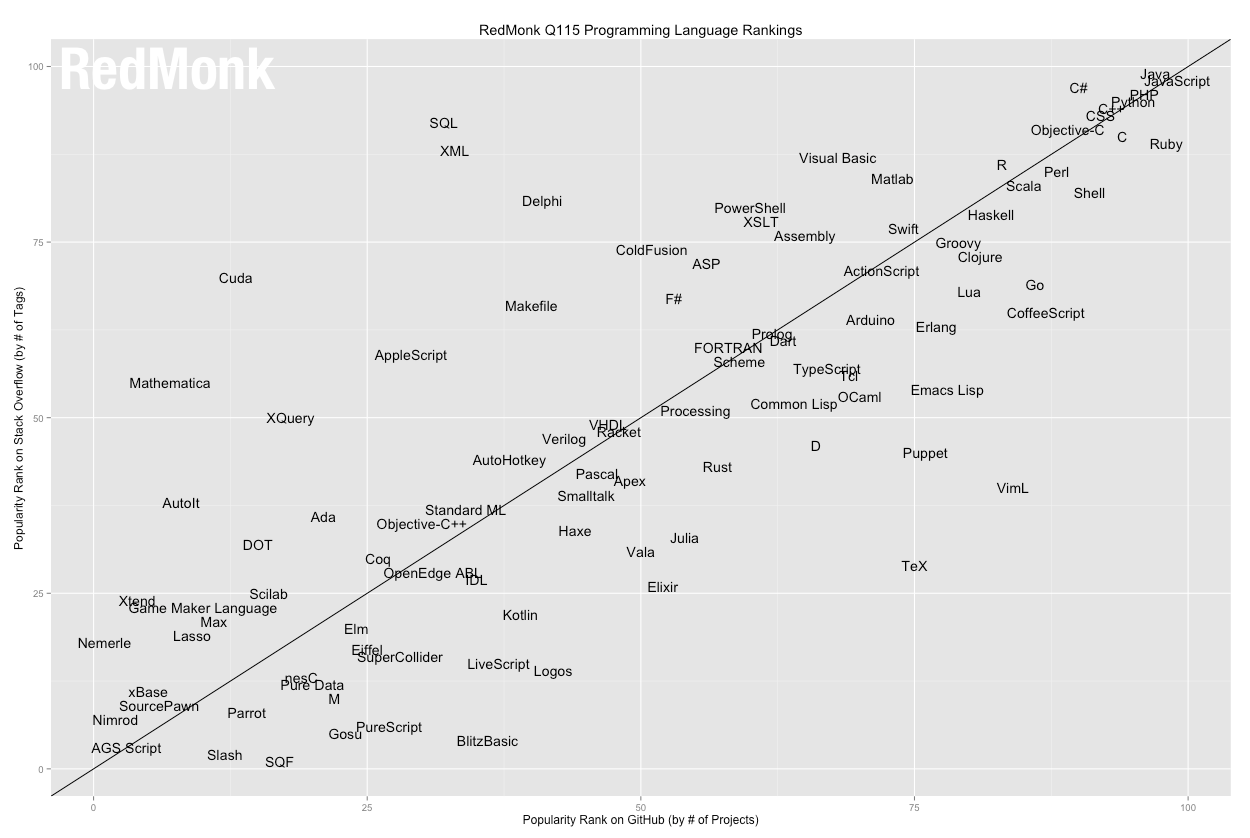
\includegraphics[width=1\textwidth]{img/grafico_redmonk}
	\caption{Ranking das liguagens de programação no Stack Overflow e Github}
\end{figure}


Ainda assim, para compor a interface do dado projeto, também ocorrerá o uso do líder JavaScript de forma intensa, provendo o elo com o as informações gerenciadas pelo PHP.


Entretanto, não seria inteligente desenvolver um sistema completo sem o auxílio de um framework. Dentre os frameworks disponíveis para PHP, hoje o destaque está com o Laravel, que se encontra no topo dentre os mais utilizados no momento. 


A WebHostFace, uma empresa de hospedagem, compilou várias estatísticas para criar um infográfico mostrando os frameworks PHP mais populares de 2015. Utilizando informações sobre os próprios clientes, o Google Trends, estatísticas de repositórios do GitHub e a pesquisa do SitePoint “Best PHP Frameworks 2015”, a WebHostFace elaborou o seguinte infográfico: 

\begin{figure}
	\label{fig:graficoWebhostface}
	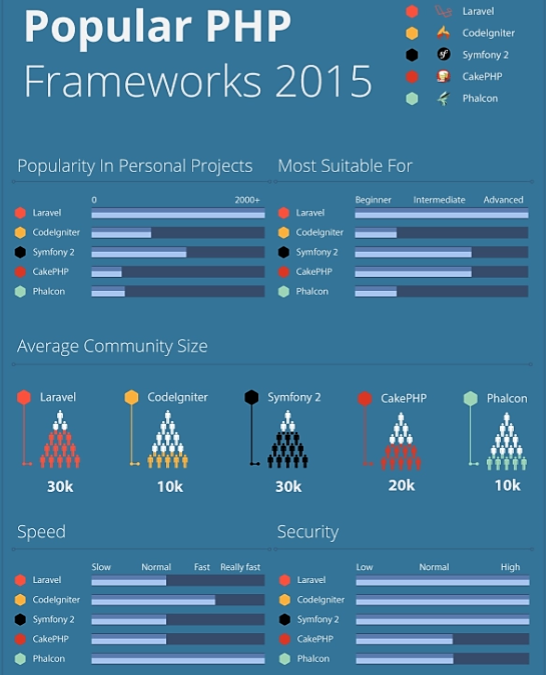
\includegraphics[width=1\textwidth]{img/infografico_webhostface}
	\caption{Infográfico da WebhostFace, exibindo a popularidade dos Frameworks PHP em 2015}
\end{figure}

Assim, tem-se a evidência que o Laravel em 2015 teve a maior popularidade em projetos pessoais e tem a maior comunidade entre os concorrentes, o que o torna uma boa escolha para a escrita de um software que será continuado por terceiros.


Para elaborar os recursos de interface e integrar ao back-end PHP do sistema, será adotado o já conhecido AngularJS, ferramenta sólida e conhecida no aspecto em questão. 


Dados coletados via Google Trends, que propõe comparações entre termos pesquisados, revela a popularidade do AngularJs diante de alguns dos principais concorrentes. O gráfico abaixo evidencia o cenário.


%Como mostra a Figura \ref{fig:graficoGoogleTrendsFerramentasFront}. 
\begin{figure}
	\label{fig:graficoGoogleTrendsFerramentasFront}
	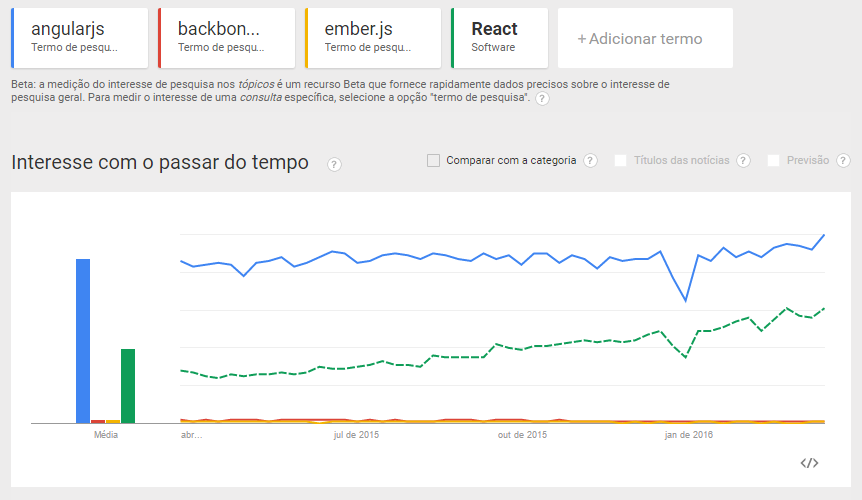
\includegraphics[width=1\textwidth]{img/grafico_ferramentas_front}
	\caption{Gráfico do Google Trends exibindo as pesquisas por ferramentas front-end}
\end{figure}


Junto ao Angular JS, será utilizada a agradável tendência de interface do Material Design da Google, que propõe layouts limpos e otimizados já conhecidos pelos usuários de smartphones Android. 


Para a elaboração da plataforma mobile do projeto, será utilizado o Ionic Framework, muito difundido e bastante pesquisado na área, o que fica evidenciado com o gráfico de pesquisbaixo, coletado via Google Trends buscando por frameworks de desenvolvimento híbrido mobile.


\begin{figure}
	\label{fig:graficoGoogleTrendsFerramentasHibridasMobile}
	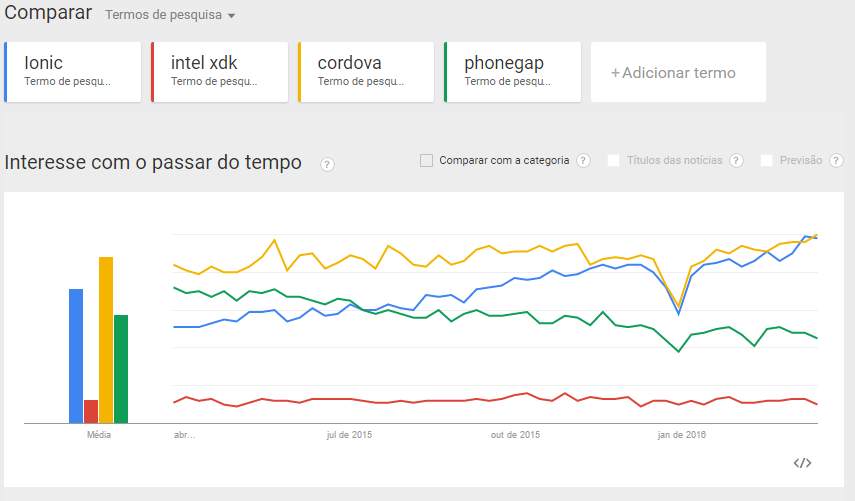
\includegraphics[width=1\textwidth]{img/grafico_ferramentas_hibridas_mobile}
	\caption{Gráfico do Google Trends exibindo as pesquisas por Frameworks híbridos mobile}
\end{figure}	

Para layout da interface mobile, também será aplicado a tendência do Material Design, a fim de propor uma harmonia entre o módulo web e mobile para os usuários


\section{Resultados Esperados}


Como fruto de um sistema para pós-graduação da UFBA, espera-se que os professores tenham mais recursos para integrar as atividades e também prover melhores condições para acompanhamento da vida acadêmica dos alunos em questão. Também, que os novos colaboradores que entrarem no processo tenham facilidade de compreender o fluxo do setor ao navegar pelo sistema proposto.


\section{Fora de Escopo}


Interação com os alunos devido às complicações para realizar a integração com o sistema empregado na UFBA, gerenciado pela XXXXXX, o que causaria uma inviabilidade no projeto devido à necessidade de entrega do produto ser mais forte que o tempo necessário para executar o processo de obtenção de acesso ao sistema legado para realizar a integração.


\section{Estrutura do Trabalho}


<breve resumo sobre os capítulos do TCC>
\chapter{Referencial Teórico}


Projetar o desenvolvimento de um software requer muito planejamento, pois as falhas iniciais podem custar bastante caro ou até mesmo inviabilizar a continuação de um projeto. Assim, a escolha da arquitetura ideal para a aplicabilidade é essencial na concepção de um produto de software. 
De todo o modo, sempre busca-se fazer mais com menos. Diante de tal filosofia, temos nesta seção, uma breve discussão sobre alguns elementos de projeto e arquitetura de software, a fim de contextualizar este trabalho de conclusão de curso.


% Ser direto no começo, focando no que realmente será discutido A seção \ref{sec:apps_mobile} 
 \section{Software como serviço}\label{sec:saas}


A definição de SaaS encontra-se muito bem elaborada em um dos trabalhos listados na literatura. Segundo La e Chun \citep{La2009Systematic}, o princípio da definição de Software como um Serviço (Sofware as a Service - SaaS) é um serviço complementar para aplicações da computação em nuvem (cloud computing). As duas áreas estão interligadas, no entanto, não se confundem, pois o SaaS deve ser entendido como um mecanismo de suporte às soluções existentes na cloud. Os SaaS existem justamente para maximizar o reuso de serviços repetidos e não centrais em uma aplicação remota.


Como propõe vantagens, software como servico é uma tendência forte, isso graças à evolução da web. Diversos fatores podem ser favoráveis para a adoção de um SaaS, como custo e manutenção dentre outros fatores aplicaveis a determinados contextos. Um trabalho recente realizado por Lechessa et al. \cite{LechesaSS11} apresenta uma pesquisa qualitativa sobre os fatores determinantes para adoção ou não de um SaaS voltado para ERP na África do Sul. Esses autores indicam que os principais fatores determinantes para adoção desse mecanismo de software são sua fluidez quanto à rede e a segurança. Esses fatores estão presentes na aplicação desenvolvida neste trabalho de conclusão de curso.
 

Devido ao fato de ter um serviço constantemente na nuvem, fica o questionamento sobre a segurança da informação manipulada. Sabe-se que a vulnerabilidade na web não é restrita ao SaaS, atingindo diversos âmbitos. O artigo de Rai et al. \cite{journals/corr/RaiSM13} orienta como o avanço da computação em nuvem não é um problema apenas para os serviços web do ponto de vista da segurança, pois muitos trabalhos na literatura mostram a área como mais um ponto de vulnerabilidade para diversos setores, a exemplo de infraestrutura. No mesmo artigo mencionado de Rai et al. \cite{journals/corr/RaiSM13}, também realizaram-se estudos exploratórios junto a empresas usuárias de serviços em computação em nuvem e consideram que a perspectiva de SaaS também pode fortalecer a segurança nas aplicações de cloud computing, pois o software de autenticação compartilhado por várias aplicações em nuvem, oferece uma melhor padronização e consequente facilidade de prevenção a erros de vulnerabilidade específicas de cada módulo da pesquisa. Esse ponto de vista é muito importante para qualquer trabalho de ponta na área de SaaS.


A arquitetura de armazenamento de dados de um Saas pode variar de acordo com a necessidade do contexto. O artigo recente de Huixin \cite{7586486}, exemplifica possíveis modelagens para utilizar. Tal abordagem pode ser com um banco de dados único, fazendo com que diferentes clientes compartilhem o mesmo banco, diferindo os dados através de controle de usuário, ou isolando os diferentes clientes através de bancos de dados exclusivos para cada um. Tal fator também pode ser combinado com a arquitetura da aplicação, caso ofereça aplicação única para todos os clientes ou aplicação compartilhada. Diante das possíveis abprdagens, a modelagem de dados do software pode ser decidida pela regra de negócio. Este trabalho optou por aplicação única e banco de dados compartilhado.


Devido ao diferente conceito de obtenção de software, tanto pela visão do cliente como pela visão do vendedor, é necessário tomar conhecimento dos diversos fatores que podem ser relevantes ao orçar um Saas. O recente trabalho de T. Kaur et al. \citep{6949281} orienta um modelo para compor o custo de um Saas. O custo total seria composto pelos fatores que dão suporte ao funcionamento do software. Tais fatores incluem infra-estrutura, configurabilidade, customização, parâmetros de QoS(Quality of service) como escalabilidade, disponibilidade, usabilidade, pontualidade e desempenho da resposta, portabilidade, custo total de propriedade e retorno do investimento. Esses fatores caracterizam o custo de forma eficaz, possibilitando ao fornecedor, prover um Serviço de acordo com a exigência do consumidor em vários pacotes de serviços.


\section{Reuso de software}\label{sec:reuso} %CRUISE BOOK CAPITULO 2


Para Peter Freeman, o reuso é a utilização de qualquer informação que um desenvolvedor pode necessitar no processo de criação de software (Ezran et al., 2002). Basili e Rombach definem reutilização de software como o uso de tudo o que está associado a um projeto de conhecimento (Basili e Rombach, 1991).
Assim, o objetivo da reutilização de software é reciclar o design, código e outros componentes de um produto de software e assim reduzir o custo, o tempo e melhorar a qualidade do produto.
Segundo Keswani et al. \cite{6783445}, o componente reutilizável de software pode ser qualquer parte de seu desenvolvimento, como um fragmento de código, design, casos de teste, ou até mesmo a especificação de requisitos de uma funcionalidade do software. 

O reuso de software pode ter impacto positivo em diversos aspectos do software, vejamos alguns, conforme apresentados no C.R.U.I.S.E Book:

\begin{itemize}

\item Qualidade: As correções de erro tornam-se úteis em todos os locais em que ocorreu, padronizando e facilitando a manutenção.

\item Produtividade: O ganho de produtividade é alcançado devido ao menor número de artefatos desenvolvido. Isso resulta em menos esforços de teste e também economiza análise e design, gerando economia em diversos escopos do projeto.

\item Confiabilidade: A utilização de componentes bem testados aumenta a
confiança no software. Além disso, a utilização de um mesmo componente em vários sistemas, aumenta a possibilidade de detecção de erros e reforça a confiança no componente.

\item Redução do Esforço: A reutilização de software proporciona uma redução do tempo de desenvolvimento, o que reduz o tempo necessário para o produto ser disponibilizado no mercado para trazer rentabilidade.

\item Trabalho redundante e tempo de desenvolvimento: Desenvolver um sistema do
zero significa desenvolvimento redundante de muitos componentes, como requisito
especificações, casos de uso, arquitetura, etc. Isso pode ser evitado quando estes estão disponíveis como componentes reutilizáveis e podem ser compartilhados, resultando em menos desenvolvimento, tempo e custo associado.

\item Documentação: Embora a documentação seja muito importante para a
manutenção de um sistema, muitas vezes é negligenciada. A reutilização de componentes software reduz a quantidade de documentação a ser escrita, entretanto depende da qualidade do que está escrito. Assim, apenas a estrutura do sistema e os novos artefatos desenvolvidos necessitam ser documentados.

\item Custo de manutenção: Menos defeitos e manutenções são esperados quando tem-se comprovada a qualidade dos componentes utilizados.

\item Tamanho da equipe: É comum entrar casos em que a equipe de desenvolvimento sofre sobrecarga. Entretanto, dobrar o tamanho da equipe de desenvolvimento não necessariamente duplica produtividade. Se muitos componentes podem ser reutilizados, é possível desenvolver com equipes menores, levando a melhores comunicações e aumento da produtividade.

\end{itemize}

Apesar dos benefícios da reutilização de software, a mesma não é amplamente praticado como imagina-se. Existem fatores que influenciam direta ou indiretamente na sua adoção. Esses fatores podem ser de aspecto gerencial, organizacional, econômico, conceitual ou técnico. Veremos a seguir alguns aspectos que podem gerar conflito com a cultura de reuso de software, segundo o C.R.U.I.S.E Book:
%(Sametinger, 1997). REVER

\begin{itemize}
	
\item Falta de apoio da gestão: Como a reutilização de software gera custos iniciais,
a medida pode não ser amplamente alcançada em uma organização sem o apoio de alto nível gestão. Os gestores têm de ser informados sobre os custos iniciais e serem convencidos sobre economias futuras.

\item Gerenciamento do Projeto: Gerenciar projetos tradicionais é uma tarefa árdua, principalmente, os que praticam a reutilização de software. Utilizando a técnica em larga escala, tem-se impacto sobre todo o ciclo de vida do software.

\item Estruturas organizacionais inadequadas: As estruturas organizacionais devem
considerar diferentes necessidades que surgem quando a reutilização em larga escala está sendo adotada. Por exemplo, uma equipe particionada pode ser alocada somente para desenvolver, manter e certificar componentes reutilizáveis de software.

\item Incentivos de gestão: É comum a falta de incentivo para deixar os desenvolvedores gastarem tempo elaborando reutilizáveis componentes do sistema. A produtividade é muitas vezes medida apenas no tempo necessário para concluir um projeto. Assim, fazer qualquer trabalho além disso, embora benéfico para a empresa como um todo, diminui o seu sucesso. Mesmo quando os componentes reutilizáveis são utilizados, os benefícios obtidos são uma pequena fração do que poderia ser alcançado caso houvesse reutilização explícita, planejada e organizada.

\item Dificuldade de encontrar software reutilizável: Para reutilizar os componentes, devem existir formas eficientes de busca. Além disso, é importante ter um repositório bem organizado contendo componentes com um eficiente meio de acesso.

\item Não reutilização do software encontrado. O acesso fácil ao software existente
não necessariamente aumentar a reutilização. Os componentes reutilizáveis devem ser cuidadosamente especificados, projetados, implementados e documentados, pois em alguns casos, modificar e adaptar o código  pode ser mais custoso que a programação da funcionalidade necessária a partir do zero.

\item Modificação: É muito difícil encontrar um componente que funcione
exatamente da mesma maneira que queremos. Desta forma, são necessárias modificações e devem existir formas de determinar os seus efeitos sobre o componente.


\end{itemize}


%Outra diretriz importante para a reutilização de software é reduzir o risco na criação de novos softwares. O risco tende a ser bastante reduzido se os componentes que estão sendo reutilizados têm as documentação, interfaces necessárias e devidamente testadas, fatores que contibruem para uma fácil integração.
%De acordo com Keswani et al. \citep{6783445}, para o reuso de software dar retornos apropriados, o processo deve ser sistemático e planejado. Qualquer organização que implemente a reutilização de software deve identificar os melhores métodos e estratégias de reutilização para obter a máxima produtividade. A reutilização de software ajuda a evitar software de engenharia a partir do zero, pois usa módulos de software existentes. A reutilização de software, embora seja uma tarefa difícil, especialmente para softwares antigos sem padrões de projeto, pode melhorar significativamente a produtividade e a qualidade de um produto de software. Embora a reutilização de software não seja um novo campo, ela pode dar grandes retornos em curto período de tempo.


\section{Modularização}\label{sec:modularizacao} %artigo de claudio pagina 222 introdução


%A modularidade vem desempenhando um papel predominante estágios emergentes das disciplinas de arquitetura de software [13]. Engenheiros de software consideram modularidade como princípio base na comparação entre arquiteturas alternativas  e arquitetura degeneração [9]. De fato, os engenheiros de software são incentivados a arquitecturas, baseando-se numa multiplicidade de mecanismos de modularidade disponíveis em: 
%(i) Linguagens de descrição de arquitetura (ADLs), como ACME [8], 
%(ii) catálogos de arquitetônicos [2, 13], e 
%(iii) conhecem bem princípios de alto nível, como interfaces de componentes estreitos, acoplamento arquitectónico reduzido e semelhantes.


Conforme é frisado no trabalho de Wickramaarachchi e Lai \citep{7062705}, o conceito de modularização na indústria de software tem uma longa história e tem sido utilizado para melhorar o processo de desenvolvimento de software em diferentes estágios. Os principais conceitos por trás da modularização do software foram introduzidos por pesquisadores pioneiros há quarenta anos, com uma notável contribuição feita por Melvin Conway e David Parnas, que tem representação notável na engenharia de software.


Modularizar um software é um bom padrão a ser adotado. Segundo Wickramaarachchi e Lai \citep{7062705}, a modularização é importante na identificação de dependências e reduz as dificuldades diante de uma possível necessidade de grandes alterações. De uma perspectiva da engenharia de software, uma modularização geralmente tem várias vantagens, tais como: tornar a complexidade do software mais gerenciável, facilitar o trabalho paralelo e tornar o software mais maleável para acomodar o futuro incerto que um software pode ter. O objetivo final da modularização do software é aumentar a produtividade ea qualidade do software. Tal conceito encontra-se bastante difundido e estái incorporado em linguagens de programação e ferramentas de software. O trabalho proposto favorece ao uso da modularização de um software e até mesmo pode ser considerado um módulo a ser acoplado a qualquer software, mediante a compatibilidade.


\section{Aplicações web}\label{sec:apps_web}


A popularidade da aplicação web aumentou exponencialmente na última década e todos os dias cresce o número de pessoas usuárias de aplicações web. E seguindo o padrão de desenvolvimento de software, Kumar et al. \citep{7813710} sugerem que para o desenvolvimento web, deve-se manter a prática efiacaz de produzir diagramas UML. A abordagem baseada na web oferece uma maneira fácil e eficaz para gerenciar e controlar o processo de desenvolvimento por meio de diagramas UML. Tal abordagem pode ser usada quando há uma exigência de lidar com mudanças muito rápidas e grandes em requisitos de forma muito eficaz em muito menos tempo, gerando assim um menor impacto. 


Para atender à fomentada demanda de aplicativos web, é necessário adotar métodos de desenvolvimentos que sejam ágeis, eficientes e de fácil manutenção. Yu Ping et al. \cite{1372143} propõem o uso do modelo MVC (Model, View e Controller) no atual desenvolvimento para softwares web. O modelo apresentado tornou-se um padrão popular e divide o software em camadas com propósito definido, tornando-o de mais fácil manutenção.


O Ajax (Asynchronous Javascript and XML) revolucionou a web. Conforme demonstrado no artigo de Yuping \citep{6845605}, ao usar a tecnologia Ajax, podemos enriquecer a experiência do usuário em aplicações baseadas em navegador de internet, e fornecer uma variedade de aplicações interativas para atender às necessidade de humanização das aplicações.
Os aplicativos Ajax em execução no navegador se comunicam com um servidor Web de forma assíncrona e atualizam apenas uma parte da página.



% %% RiSE Latex Template - version 0.5
%%
%% RiSE's latex template for thesis and dissertations
%% http://risetemplate.sourceforge.net
%%
%% (c) 2012 Yguaratã Cerqueira Cavalcanti (yguarata@gmail.com)
%%          Vinicius Cardoso Garcia (vinicius.garcia@gmail.com)
%%
%% This document was initially based on UFPEThesis template, from Paulo Gustavo
%% S. Fonseca.
%%
%% ACKNOWLEDGEMENTS
%%
%% We would like to thanks the RiSE's researchers community, the 
%% students from Federal University of Pernambuco, and other users that have
%% been contributing to this projects with comments and patches.
%%
%% GENERAL INSTRUCTIONS
%%
%% We strongly recommend you to compile your documents using pdflatex command.
%% It is also recommend use the texlipse plugin for Eclipse to edit your documents.
%%
%% Options for \documentclass command:
%%         * Idiom
%%           pt   - Portguese (default)
%%           en   - English
%%
%%         * Text type
%%           bsc  - B.Sc. Thesis
%%           msc  - M.Sc. Thesis (default)
%%           qual - PHD qualification (not tested yet)
%%           prop - PHD proposal (not tested yet)
%%           phd  - PHD thesis
%%
%%         * Media
%%           scr  - to eletronic version (PDF) / see the users guide
%%
%%         * Pagination
%%           oneside - unique face press
%%           twoside - two faces press
%%
%%		   * Line spacing
%%           singlespacing  - the same as using \linespread{1}
%%           onehalfspacing - the same as using \linespread{1.3}
%%           doublespacing  - the same as using \linespread{1.6}
%%
%% Reference commands. Use the following commands to make references in your
%% text:
%%          \figref  -- for Figure reference
%%          \tabref  -- for Table reference
%%          \eqnref  -- for equation reference
%%          \chapref -- for chapter reference
%%          \secref  -- for section reference
%%          \appref  -- for appendix reference
%%          \axiref  -- for axiom reference
%%          \conjref -- for conjecture reference
%%          \defref  -- for definition reference
%%          \lemref  -- for lemma reference
%%          \theoref -- for theorem reference
%%          \corref  -- for corollary reference
%%          \propref -- for proprosition reference
%%          \pgref   -- for page reference
%%
%%          Example: See \chapref{chap:introduction}. It will produce 
%%                   'See Chapter 1', in case of English language.

\documentclass[pt,twoside,onehalfspacing,bsc]{risethesis}

\usepackage[utf8]{inputenc}
\usepackage[brazilian]{babel}
\usepackage[T1]{fontenc}

%% Change the following pdf author attribute name to your name.
\usepackage[linkcolor=blue,citecolor=blue,urlcolor=blue,colorlinks,pdfpagelabels,pdftitle={Bruno Cabral's Bachelor Thesis},pdfauthor={Bruno Cabral}]{hyperref}

\address{SALVADOR}

\universitypt{Universidade Federal da Bahia}
\universityen{Federal University of Bahia}

\departmentpt{Depertamento de Ciência da Computação}
\departmenten{Computer Science Department}

\programpt{Programa Multiinstitucional de Pós-graduação em Ciência da Computação}
\programen{Graduate in Computer Science}

\majorfieldpt{Ciência da Computação}
\majorfielden{Computer Science}

\title{Sistema de apoio à Pós graduação - UFBA}
\date{Outubro/2016}

\author{Victor de Azevedo Nunes}
\adviser{Ivan do Carmo Machado}

\begin{document}

\frontmatter
\frontpage
\presentationpage

\begin{dedicatory}
Eu dedico esta dissertação...
%I dedicate this dissertation to my family, girlfriend, friends and
%professors who gave me all necessary support to get here.
\end{dedicatory}

\acknowledgements
Meus agradecimentos...

\begin{epigraph}[]{Edward V Berard}
Walking on water and developing software from a specification are easy if both are frozen
\end{epigraph}

\resumo
% Escreva seu resumo no arquivo resumo.tex
Meu resumo

\begin{keywords}
palavras chave

\end{keywords}

\abstract
% Write your abstract in a file called abstract.tex
My abstract...

\begin{keywords}
key words...
\end{keywords}

% Summary (tables of contents)
\tableofcontents

% List of figures
\listoffigures

% List of tables
\listoftables

% List of acronyms
% Acronyms manual: http://linorg.usp.br/CTAN/macros/latex/contrib/acronym/acronym.pdf
\listofacronyms
\begin{acronym}[ACRONYM] 
% Change the word ACRONYM above to change the acronym column width.
% The column width is equals to the width of the word that you put.
% Read the manual about acronym package for more examples:
%   http://linorg.usp.br/CTAN/macros/latex/contrib/acronym/acronym.pdf

\acro{SPA}{Single Page Application}
\acro{JSON}{Javascript Object Notation}
\acro{PHP}{PHP: Hypertext Preprocessor}
\acro{SaaS}{Software as a Service}
\acro{ERP}{Enterprise Resource Planning}
\acro{QoS}{Quality of Service}
\acro{UML}{Unified Modeling Language}
\acro{MVC}{Model-View-Controller}
\acro{Ajax}{Asynchronous Javascript and XML}
\acro{HTML}{HyperText Markup Language}
\acro{CSS}{Cascading Style Sheets}
\acro{API}{Application Programming Interface}
\acro{DOM}{Document Object Model}
\acro{BPMN}{Business Process Model and Notation}
\acro{REST}{Representational State Transfer}

\end{acronym}

% List of listings
%\lstlistoflistings

\mainmatter

\chapter{Introdução}

\section{Motivação}

Organizar os procedimentos de um processo sempre nos traz vantagens. Apesar de no processo de implantação de um sistema, o mesmo burocratizar o processo, com o tempo temos o retorno da dedicação para a inserção dos dados. Com um certo volume de dados, é possível estruturar informações que num processo manual são difíceis de serem enxergadas. Assim, é possível depender menos das pessoas que organizam o processo, pois o legado de informações não estará mais somente na mente de alguns, mas sim documentado nos dados do sistema.

Além de colaborar na organização, também haverá uma grande colaboração no tempo gasto na gestão. Lidar com muitos papéis e confiar na mente humana para guardar informações, não é uma alternativa muito segura devido ao fato que as pessoas sempre estão sujeitas a sair do processo e levar contigo a experiência obtida. Experiência essa que faz com que os procedimentos sejam executados de forma mais eficiente. Entretanto, com um sistema inteligente, é possível auxiliar e tornar mais ágil a execução das tarefas.


\section{Problema}


De acordo com funcionários ligados ao o setor de pós graduação da UFBA, entrevistados a fim de um maior entendimento do cenário, apesar das semelhanças estruturais, a pós graduação gerida de forma diferencia da graduação. FULANO afirma que devido ao fato de não ter a mesma visibilidade, não tem acesso aos mesmos recursos de gestão acadêmica da graduação. O professores não executam somente atividades dentro da sala de aula, também tem diversas outras ocupações no setor. E muitos procedimentos realizados extra classe ainda se encontram sendo realizados de forma manual, estando mais vulnerável ao erro ou até mesmo à violação do processo. Também ocorre um grande desperdício de tempo pelos professores e gestores da área, devido ao diversos processos ainda realizados de forma manual, sem a devida documentação. Segundo FULANO, também entrevistado, esse tempo perdido implica numa redução da eficiência na sala de aula, pois o professor acaba por ter menos tempo disponível para o planejamento das atividades, o que gera impactos negativos aos alunos.


\section{Objetivos} %<o que deve ser feito/entregue>


Devido aos muitos processos sendo resolvidos de forma manual, propõe-se com solução um sistema moderno, arquitetado para ter funcionamento na web e com um módulo mobile, a fim de fornecer informações de forma rápida e eficiente para os professores através de notificações, já que o acesso à internet móvel é comum entre os possíveis usuários do sistema em questão.
O principal requisito para o sistema seria dispor recursos para reduzir o tempo desperdiçado pelos professores durante as atividades extra classe.


\section{Metodologia} %<como será feito | como resolver o problema apontado inicialmente>


%<analise de literatura | design | implementação | validação>
Baseando-se nas tecnologias gratuitas em alta no cenário atual do desenvolvimento web, dispomos de algumas opções eficientes para a implementação da solução. Dentre as possibilidades, considerando a facilidade para futura manutenção e continuidade do projeto, tende-se a optar por uma tecnologia popular. Como linguagem de programação, adota-se o PHP. A escolha é fundamentada de acordo com a pesquisa da RedMonk de 2015, que evidencia o uso das linguagens de programação de acordo com as discussões no StackOverflow e repositórios no GitHub. É possível constatar a popularidade do PHP no cenário atual com o gráfico da pesquisa citada, na qual o PHP é apresentado na terceira colocação, apenas atrás do lider JavaScript e do segundo colocado, o Java.

\begin{figure}
	\label{fig:graficoRedmonk}
	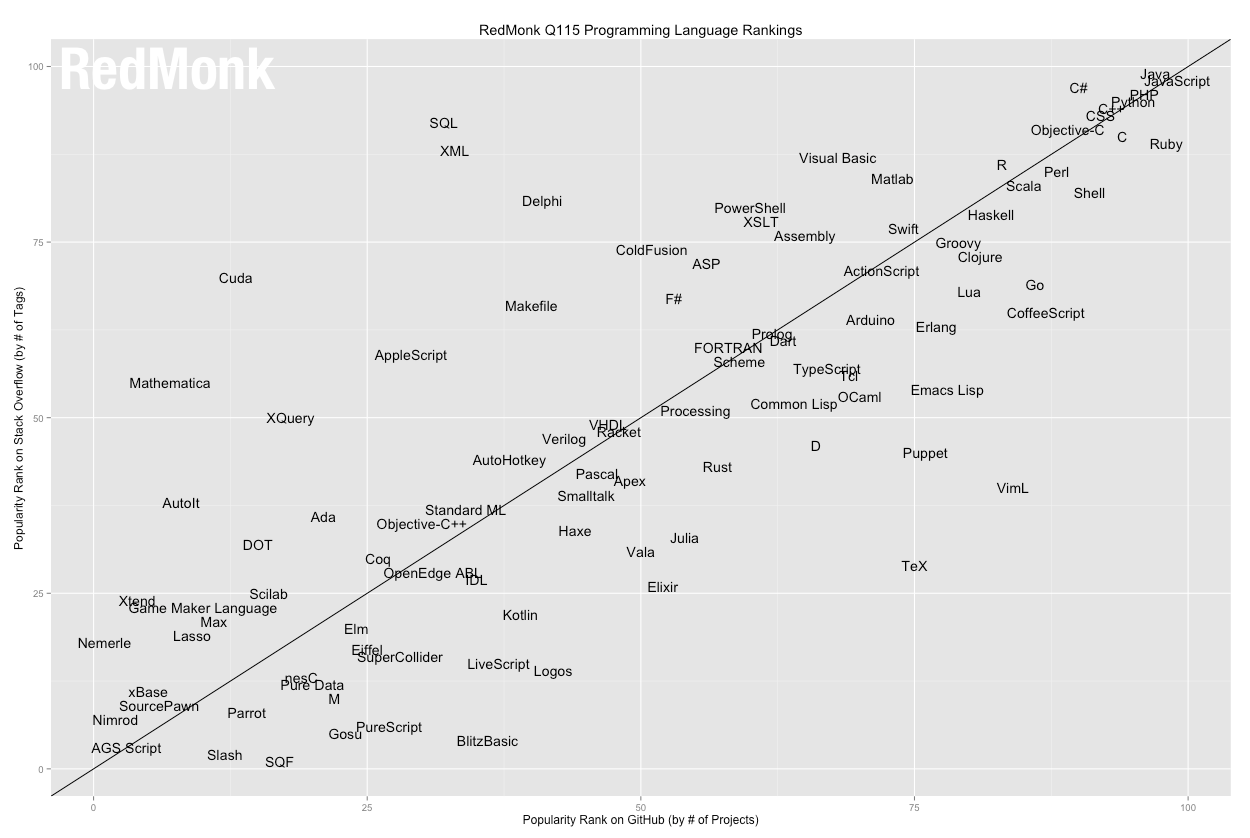
\includegraphics[width=1\textwidth]{img/grafico_redmonk}
	\caption{Ranking das liguagens de programação no Stack Overflow e Github}
\end{figure}


Ainda assim, para compor a interface do dado projeto, também ocorrerá o uso do líder JavaScript de forma intensa, provendo o elo com o as informações gerenciadas pelo PHP.


Entretanto, não seria inteligente desenvolver um sistema completo sem o auxílio de um framework. Dentre os frameworks disponíveis para PHP, hoje o destaque está com o Laravel, que se encontra no topo dentre os mais utilizados no momento. 


A WebHostFace, uma empresa de hospedagem, compilou várias estatísticas para criar um infográfico mostrando os frameworks PHP mais populares de 2015. Utilizando informações sobre os próprios clientes, o Google Trends, estatísticas de repositórios do GitHub e a pesquisa do SitePoint “Best PHP Frameworks 2015”, a WebHostFace elaborou o seguinte infográfico: 

\begin{figure}
	\label{fig:graficoWebhostface}
	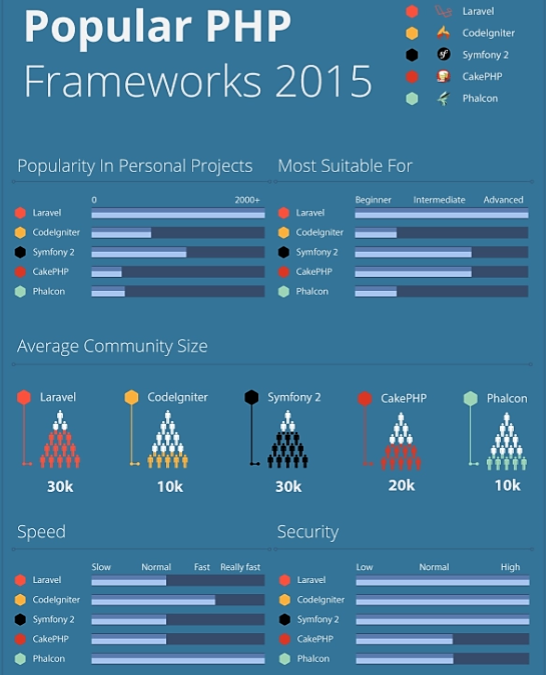
\includegraphics[width=1\textwidth]{img/infografico_webhostface}
	\caption{Infográfico da WebhostFace, exibindo a popularidade dos Frameworks PHP em 2015}
\end{figure}

Assim, tem-se a evidência que o Laravel em 2015 teve a maior popularidade em projetos pessoais e tem a maior comunidade entre os concorrentes, o que o torna uma boa escolha para a escrita de um software que será continuado por terceiros.


Para elaborar os recursos de interface e integrar ao back-end PHP do sistema, será adotado o já conhecido AngularJS, ferramenta sólida e conhecida no aspecto em questão. 


Dados coletados via Google Trends, que propõe comparações entre termos pesquisados, revela a popularidade do AngularJs diante de alguns dos principais concorrentes. O gráfico abaixo evidencia o cenário.


%Como mostra a Figura \ref{fig:graficoGoogleTrendsFerramentasFront}. 
\begin{figure}
	\label{fig:graficoGoogleTrendsFerramentasFront}
	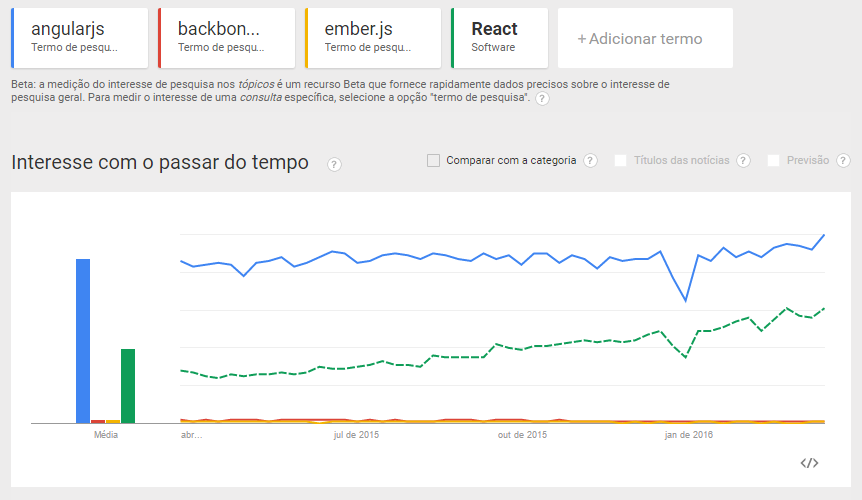
\includegraphics[width=1\textwidth]{img/grafico_ferramentas_front}
	\caption{Gráfico do Google Trends exibindo as pesquisas por ferramentas front-end}
\end{figure}


Junto ao Angular JS, será utilizada a agradável tendência de interface do Material Design da Google, que propõe layouts limpos e otimizados já conhecidos pelos usuários de smartphones Android. 


Para a elaboração da plataforma mobile do projeto, será utilizado o Ionic Framework, muito difundido e bastante pesquisado na área, o que fica evidenciado com o gráfico de pesquisbaixo, coletado via Google Trends buscando por frameworks de desenvolvimento híbrido mobile.


\begin{figure}
	\label{fig:graficoGoogleTrendsFerramentasHibridasMobile}
	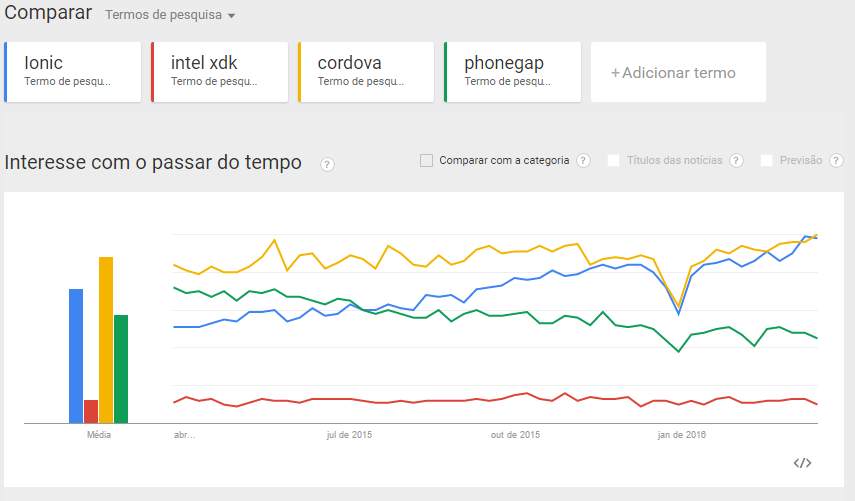
\includegraphics[width=1\textwidth]{img/grafico_ferramentas_hibridas_mobile}
	\caption{Gráfico do Google Trends exibindo as pesquisas por Frameworks híbridos mobile}
\end{figure}	

Para layout da interface mobile, também será aplicado a tendência do Material Design, a fim de propor uma harmonia entre o módulo web e mobile para os usuários


\section{Resultados Esperados}


Como fruto de um sistema para pós-graduação da UFBA, espera-se que os professores tenham mais recursos para integrar as atividades e também prover melhores condições para acompanhamento da vida acadêmica dos alunos em questão. Também, que os novos colaboradores que entrarem no processo tenham facilidade de compreender o fluxo do setor ao navegar pelo sistema proposto.


\section{Fora de Escopo}


Interação com os alunos devido às complicações para realizar a integração com o sistema empregado na UFBA, gerenciado pela XXXXXX, o que causaria uma inviabilidade no projeto devido à necessidade de entrega do produto ser mais forte que o tempo necessário para executar o processo de obtenção de acesso ao sistema legado para realizar a integração.


\section{Estrutura do Trabalho}


<breve resumo sobre os capítulos do TCC>
\chapter{Referencial Teórico}


Projetar o desenvolvimento de um software requer muito planejamento, pois as falhas iniciais podem custar bastante caro ou até mesmo inviabilizar a continuação de um projeto. Assim, a escolha da arquitetura ideal para a aplicabilidade é essencial na concepção de um produto de software. 
De todo o modo, sempre busca-se fazer mais com menos. Diante de tal filosofia, temos nesta seção, uma breve discussão sobre alguns elementos de projeto e arquitetura de software, a fim de contextualizar este trabalho de conclusão de curso.


% Ser direto no começo, focando no que realmente será discutido A seção \ref{sec:apps_mobile} 
 \section{Software como serviço}\label{sec:saas}


A definição de SaaS encontra-se muito bem elaborada em um dos trabalhos listados na literatura. Segundo La e Chun \citep{La2009Systematic}, o princípio da definição de Software como um Serviço (Sofware as a Service - SaaS) é um serviço complementar para aplicações da computação em nuvem (cloud computing). As duas áreas estão interligadas, no entanto, não se confundem, pois o SaaS deve ser entendido como um mecanismo de suporte às soluções existentes na cloud. Os SaaS existem justamente para maximizar o reuso de serviços repetidos e não centrais em uma aplicação remota.


Como propõe vantagens, software como servico é uma tendência forte, isso graças à evolução da web. Diversos fatores podem ser favoráveis para a adoção de um SaaS, como custo e manutenção dentre outros fatores aplicaveis a determinados contextos. Um trabalho recente realizado por Lechessa et al. \cite{LechesaSS11} apresenta uma pesquisa qualitativa sobre os fatores determinantes para adoção ou não de um SaaS voltado para ERP na África do Sul. Esses autores indicam que os principais fatores determinantes para adoção desse mecanismo de software são sua fluidez quanto à rede e a segurança. Esses fatores estão presentes na aplicação desenvolvida neste trabalho de conclusão de curso.
 

Devido ao fato de ter um serviço constantemente na nuvem, fica o questionamento sobre a segurança da informação manipulada. Sabe-se que a vulnerabilidade na web não é restrita ao SaaS, atingindo diversos âmbitos. O artigo de Rai et al. \cite{journals/corr/RaiSM13} orienta como o avanço da computação em nuvem não é um problema apenas para os serviços web do ponto de vista da segurança, pois muitos trabalhos na literatura mostram a área como mais um ponto de vulnerabilidade para diversos setores, a exemplo de infraestrutura. No mesmo artigo mencionado de Rai et al. \cite{journals/corr/RaiSM13}, também realizaram-se estudos exploratórios junto a empresas usuárias de serviços em computação em nuvem e consideram que a perspectiva de SaaS também pode fortalecer a segurança nas aplicações de cloud computing, pois o software de autenticação compartilhado por várias aplicações em nuvem, oferece uma melhor padronização e consequente facilidade de prevenção a erros de vulnerabilidade específicas de cada módulo da pesquisa. Esse ponto de vista é muito importante para qualquer trabalho de ponta na área de SaaS.


A arquitetura de armazenamento de dados de um Saas pode variar de acordo com a necessidade do contexto. O artigo recente de Huixin \cite{7586486}, exemplifica possíveis modelagens para utilizar. Tal abordagem pode ser com um banco de dados único, fazendo com que diferentes clientes compartilhem o mesmo banco, diferindo os dados através de controle de usuário, ou isolando os diferentes clientes através de bancos de dados exclusivos para cada um. Tal fator também pode ser combinado com a arquitetura da aplicação, caso ofereça aplicação única para todos os clientes ou aplicação compartilhada. Diante das possíveis abprdagens, a modelagem de dados do software pode ser decidida pela regra de negócio. Este trabalho optou por aplicação única e banco de dados compartilhado.


Devido ao diferente conceito de obtenção de software, tanto pela visão do cliente como pela visão do vendedor, é necessário tomar conhecimento dos diversos fatores que podem ser relevantes ao orçar um Saas. O recente trabalho de T. Kaur et al. \citep{6949281} orienta um modelo para compor o custo de um Saas. O custo total seria composto pelos fatores que dão suporte ao funcionamento do software. Tais fatores incluem infra-estrutura, configurabilidade, customização, parâmetros de QoS(Quality of service) como escalabilidade, disponibilidade, usabilidade, pontualidade e desempenho da resposta, portabilidade, custo total de propriedade e retorno do investimento. Esses fatores caracterizam o custo de forma eficaz, possibilitando ao fornecedor, prover um Serviço de acordo com a exigência do consumidor em vários pacotes de serviços.


\section{Reuso de software}\label{sec:reuso} %CRUISE BOOK CAPITULO 2


Para Peter Freeman, o reuso é a utilização de qualquer informação que um desenvolvedor pode necessitar no processo de criação de software (Ezran et al., 2002). Basili e Rombach definem reutilização de software como o uso de tudo o que está associado a um projeto de conhecimento (Basili e Rombach, 1991).
Assim, o objetivo da reutilização de software é reciclar o design, código e outros componentes de um produto de software e assim reduzir o custo, o tempo e melhorar a qualidade do produto.
Segundo Keswani et al. \cite{6783445}, o componente reutilizável de software pode ser qualquer parte de seu desenvolvimento, como um fragmento de código, design, casos de teste, ou até mesmo a especificação de requisitos de uma funcionalidade do software. 

O reuso de software pode ter impacto positivo em diversos aspectos do software, vejamos alguns, conforme apresentados no C.R.U.I.S.E Book:

\begin{itemize}

\item Qualidade: As correções de erro tornam-se úteis em todos os locais em que ocorreu, padronizando e facilitando a manutenção.

\item Produtividade: O ganho de produtividade é alcançado devido ao menor número de artefatos desenvolvido. Isso resulta em menos esforços de teste e também economiza análise e design, gerando economia em diversos escopos do projeto.

\item Confiabilidade: A utilização de componentes bem testados aumenta a
confiança no software. Além disso, a utilização de um mesmo componente em vários sistemas, aumenta a possibilidade de detecção de erros e reforça a confiança no componente.

\item Redução do Esforço: A reutilização de software proporciona uma redução do tempo de desenvolvimento, o que reduz o tempo necessário para o produto ser disponibilizado no mercado para trazer rentabilidade.

\item Trabalho redundante e tempo de desenvolvimento: Desenvolver um sistema do
zero significa desenvolvimento redundante de muitos componentes, como requisito
especificações, casos de uso, arquitetura, etc. Isso pode ser evitado quando estes estão disponíveis como componentes reutilizáveis e podem ser compartilhados, resultando em menos desenvolvimento, tempo e custo associado.

\item Documentação: Embora a documentação seja muito importante para a
manutenção de um sistema, muitas vezes é negligenciada. A reutilização de componentes software reduz a quantidade de documentação a ser escrita, entretanto depende da qualidade do que está escrito. Assim, apenas a estrutura do sistema e os novos artefatos desenvolvidos necessitam ser documentados.

\item Custo de manutenção: Menos defeitos e manutenções são esperados quando tem-se comprovada a qualidade dos componentes utilizados.

\item Tamanho da equipe: É comum entrar casos em que a equipe de desenvolvimento sofre sobrecarga. Entretanto, dobrar o tamanho da equipe de desenvolvimento não necessariamente duplica produtividade. Se muitos componentes podem ser reutilizados, é possível desenvolver com equipes menores, levando a melhores comunicações e aumento da produtividade.

\end{itemize}

Apesar dos benefícios da reutilização de software, a mesma não é amplamente praticado como imagina-se. Existem fatores que influenciam direta ou indiretamente na sua adoção. Esses fatores podem ser de aspecto gerencial, organizacional, econômico, conceitual ou técnico. Veremos a seguir alguns aspectos que podem gerar conflito com a cultura de reuso de software, segundo o C.R.U.I.S.E Book:
%(Sametinger, 1997). REVER

\begin{itemize}
	
\item Falta de apoio da gestão: Como a reutilização de software gera custos iniciais,
a medida pode não ser amplamente alcançada em uma organização sem o apoio de alto nível gestão. Os gestores têm de ser informados sobre os custos iniciais e serem convencidos sobre economias futuras.

\item Gerenciamento do Projeto: Gerenciar projetos tradicionais é uma tarefa árdua, principalmente, os que praticam a reutilização de software. Utilizando a técnica em larga escala, tem-se impacto sobre todo o ciclo de vida do software.

\item Estruturas organizacionais inadequadas: As estruturas organizacionais devem
considerar diferentes necessidades que surgem quando a reutilização em larga escala está sendo adotada. Por exemplo, uma equipe particionada pode ser alocada somente para desenvolver, manter e certificar componentes reutilizáveis de software.

\item Incentivos de gestão: É comum a falta de incentivo para deixar os desenvolvedores gastarem tempo elaborando reutilizáveis componentes do sistema. A produtividade é muitas vezes medida apenas no tempo necessário para concluir um projeto. Assim, fazer qualquer trabalho além disso, embora benéfico para a empresa como um todo, diminui o seu sucesso. Mesmo quando os componentes reutilizáveis são utilizados, os benefícios obtidos são uma pequena fração do que poderia ser alcançado caso houvesse reutilização explícita, planejada e organizada.

\item Dificuldade de encontrar software reutilizável: Para reutilizar os componentes, devem existir formas eficientes de busca. Além disso, é importante ter um repositório bem organizado contendo componentes com um eficiente meio de acesso.

\item Não reutilização do software encontrado. O acesso fácil ao software existente
não necessariamente aumentar a reutilização. Os componentes reutilizáveis devem ser cuidadosamente especificados, projetados, implementados e documentados, pois em alguns casos, modificar e adaptar o código  pode ser mais custoso que a programação da funcionalidade necessária a partir do zero.

\item Modificação: É muito difícil encontrar um componente que funcione
exatamente da mesma maneira que queremos. Desta forma, são necessárias modificações e devem existir formas de determinar os seus efeitos sobre o componente.


\end{itemize}


%Outra diretriz importante para a reutilização de software é reduzir o risco na criação de novos softwares. O risco tende a ser bastante reduzido se os componentes que estão sendo reutilizados têm as documentação, interfaces necessárias e devidamente testadas, fatores que contibruem para uma fácil integração.
%De acordo com Keswani et al. \citep{6783445}, para o reuso de software dar retornos apropriados, o processo deve ser sistemático e planejado. Qualquer organização que implemente a reutilização de software deve identificar os melhores métodos e estratégias de reutilização para obter a máxima produtividade. A reutilização de software ajuda a evitar software de engenharia a partir do zero, pois usa módulos de software existentes. A reutilização de software, embora seja uma tarefa difícil, especialmente para softwares antigos sem padrões de projeto, pode melhorar significativamente a produtividade e a qualidade de um produto de software. Embora a reutilização de software não seja um novo campo, ela pode dar grandes retornos em curto período de tempo.


\section{Modularização}\label{sec:modularizacao} %artigo de claudio pagina 222 introdução


%A modularidade vem desempenhando um papel predominante estágios emergentes das disciplinas de arquitetura de software [13]. Engenheiros de software consideram modularidade como princípio base na comparação entre arquiteturas alternativas  e arquitetura degeneração [9]. De fato, os engenheiros de software são incentivados a arquitecturas, baseando-se numa multiplicidade de mecanismos de modularidade disponíveis em: 
%(i) Linguagens de descrição de arquitetura (ADLs), como ACME [8], 
%(ii) catálogos de arquitetônicos [2, 13], e 
%(iii) conhecem bem princípios de alto nível, como interfaces de componentes estreitos, acoplamento arquitectónico reduzido e semelhantes.


Conforme é frisado no trabalho de Wickramaarachchi e Lai \citep{7062705}, o conceito de modularização na indústria de software tem uma longa história e tem sido utilizado para melhorar o processo de desenvolvimento de software em diferentes estágios. Os principais conceitos por trás da modularização do software foram introduzidos por pesquisadores pioneiros há quarenta anos, com uma notável contribuição feita por Melvin Conway e David Parnas, que tem representação notável na engenharia de software.


Modularizar um software é um bom padrão a ser adotado. Segundo Wickramaarachchi e Lai \citep{7062705}, a modularização é importante na identificação de dependências e reduz as dificuldades diante de uma possível necessidade de grandes alterações. De uma perspectiva da engenharia de software, uma modularização geralmente tem várias vantagens, tais como: tornar a complexidade do software mais gerenciável, facilitar o trabalho paralelo e tornar o software mais maleável para acomodar o futuro incerto que um software pode ter. O objetivo final da modularização do software é aumentar a produtividade ea qualidade do software. Tal conceito encontra-se bastante difundido e estái incorporado em linguagens de programação e ferramentas de software. O trabalho proposto favorece ao uso da modularização de um software e até mesmo pode ser considerado um módulo a ser acoplado a qualquer software, mediante a compatibilidade.


\section{Aplicações web}\label{sec:apps_web}


A popularidade da aplicação web aumentou exponencialmente na última década e todos os dias cresce o número de pessoas usuárias de aplicações web. E seguindo o padrão de desenvolvimento de software, Kumar et al. \citep{7813710} sugerem que para o desenvolvimento web, deve-se manter a prática efiacaz de produzir diagramas UML. A abordagem baseada na web oferece uma maneira fácil e eficaz para gerenciar e controlar o processo de desenvolvimento por meio de diagramas UML. Tal abordagem pode ser usada quando há uma exigência de lidar com mudanças muito rápidas e grandes em requisitos de forma muito eficaz em muito menos tempo, gerando assim um menor impacto. 


Para atender à fomentada demanda de aplicativos web, é necessário adotar métodos de desenvolvimentos que sejam ágeis, eficientes e de fácil manutenção. Yu Ping et al. \cite{1372143} propõem o uso do modelo MVC (Model, View e Controller) no atual desenvolvimento para softwares web. O modelo apresentado tornou-se um padrão popular e divide o software em camadas com propósito definido, tornando-o de mais fácil manutenção.


O Ajax (Asynchronous Javascript and XML) revolucionou a web. Conforme demonstrado no artigo de Yuping \citep{6845605}, ao usar a tecnologia Ajax, podemos enriquecer a experiência do usuário em aplicações baseadas em navegador de internet, e fornecer uma variedade de aplicações interativas para atender às necessidade de humanização das aplicações.
Os aplicativos Ajax em execução no navegador se comunicam com um servidor Web de forma assíncrona e atualizam apenas uma parte da página.



% %% RiSE Latex Template - version 0.5
%%
%% RiSE's latex template for thesis and dissertations
%% http://risetemplate.sourceforge.net
%%
%% (c) 2012 Yguaratã Cerqueira Cavalcanti (yguarata@gmail.com)
%%          Vinicius Cardoso Garcia (vinicius.garcia@gmail.com)
%%
%% This document was initially based on UFPEThesis template, from Paulo Gustavo
%% S. Fonseca.
%%
%% ACKNOWLEDGEMENTS
%%
%% We would like to thanks the RiSE's researchers community, the 
%% students from Federal University of Pernambuco, and other users that have
%% been contributing to this projects with comments and patches.
%%
%% GENERAL INSTRUCTIONS
%%
%% We strongly recommend you to compile your documents using pdflatex command.
%% It is also recommend use the texlipse plugin for Eclipse to edit your documents.
%%
%% Options for \documentclass command:
%%         * Idiom
%%           pt   - Portguese (default)
%%           en   - English
%%
%%         * Text type
%%           bsc  - B.Sc. Thesis
%%           msc  - M.Sc. Thesis (default)
%%           qual - PHD qualification (not tested yet)
%%           prop - PHD proposal (not tested yet)
%%           phd  - PHD thesis
%%
%%         * Media
%%           scr  - to eletronic version (PDF) / see the users guide
%%
%%         * Pagination
%%           oneside - unique face press
%%           twoside - two faces press
%%
%%		   * Line spacing
%%           singlespacing  - the same as using \linespread{1}
%%           onehalfspacing - the same as using \linespread{1.3}
%%           doublespacing  - the same as using \linespread{1.6}
%%
%% Reference commands. Use the following commands to make references in your
%% text:
%%          \figref  -- for Figure reference
%%          \tabref  -- for Table reference
%%          \eqnref  -- for equation reference
%%          \chapref -- for chapter reference
%%          \secref  -- for section reference
%%          \appref  -- for appendix reference
%%          \axiref  -- for axiom reference
%%          \conjref -- for conjecture reference
%%          \defref  -- for definition reference
%%          \lemref  -- for lemma reference
%%          \theoref -- for theorem reference
%%          \corref  -- for corollary reference
%%          \propref -- for proprosition reference
%%          \pgref   -- for page reference
%%
%%          Example: See \chapref{chap:introduction}. It will produce 
%%                   'See Chapter 1', in case of English language.

\documentclass[pt,twoside,onehalfspacing,bsc]{risethesis}

\usepackage[utf8]{inputenc}
\usepackage[brazilian]{babel}
\usepackage[T1]{fontenc}

%% Change the following pdf author attribute name to your name.
\usepackage[linkcolor=blue,citecolor=blue,urlcolor=blue,colorlinks,pdfpagelabels,pdftitle={Bruno Cabral's Bachelor Thesis},pdfauthor={Bruno Cabral}]{hyperref}

\address{SALVADOR}

\universitypt{Universidade Federal da Bahia}
\universityen{Federal University of Bahia}

\departmentpt{Depertamento de Ciência da Computação}
\departmenten{Computer Science Department}

\programpt{Programa Multiinstitucional de Pós-graduação em Ciência da Computação}
\programen{Graduate in Computer Science}

\majorfieldpt{Ciência da Computação}
\majorfielden{Computer Science}

\title{Sistema de apoio à Pós graduação - UFBA}
\date{Outubro/2016}

\author{Victor de Azevedo Nunes}
\adviser{Ivan do Carmo Machado}

\begin{document}

\frontmatter
\frontpage
\presentationpage

\begin{dedicatory}
Eu dedico esta dissertação...
%I dedicate this dissertation to my family, girlfriend, friends and
%professors who gave me all necessary support to get here.
\end{dedicatory}

\acknowledgements
Meus agradecimentos...

\begin{epigraph}[]{Edward V Berard}
Walking on water and developing software from a specification are easy if both are frozen
\end{epigraph}

\resumo
% Escreva seu resumo no arquivo resumo.tex
\input{resumo}

\abstract
% Write your abstract in a file called abstract.tex
\input{abstract}

% Summary (tables of contents)
\tableofcontents

% List of figures
\listoffigures

% List of tables
\listoftables

% List of acronyms
% Acronyms manual: http://linorg.usp.br/CTAN/macros/latex/contrib/acronym/acronym.pdf
\listofacronyms
\input{acronyms}

% List of listings
%\lstlistoflistings

\mainmatter

\include{chapters/intro}
\include{chapters/referencial_teorico}

% \include{chapters/introduction/main}
% \include{chapters/background/main}
% \include{chapters/proposed_solution/main}
% \include{chapters/experiment/main}
% \include{chapters/conclusion/main}

\bibliographystyle{natbib}
\addcontentsline{toc}{chapter}{\bibliographytocname}
\bibliography{references}

% Appendix
\clearpage
\addappheadtotoc
\appendix
\appendixpage
% \include{appendix/experiment-instruments}

\end{document}
% %% RiSE Latex Template - version 0.5
%%
%% RiSE's latex template for thesis and dissertations
%% http://risetemplate.sourceforge.net
%%
%% (c) 2012 Yguaratã Cerqueira Cavalcanti (yguarata@gmail.com)
%%          Vinicius Cardoso Garcia (vinicius.garcia@gmail.com)
%%
%% This document was initially based on UFPEThesis template, from Paulo Gustavo
%% S. Fonseca.
%%
%% ACKNOWLEDGEMENTS
%%
%% We would like to thanks the RiSE's researchers community, the 
%% students from Federal University of Pernambuco, and other users that have
%% been contributing to this projects with comments and patches.
%%
%% GENERAL INSTRUCTIONS
%%
%% We strongly recommend you to compile your documents using pdflatex command.
%% It is also recommend use the texlipse plugin for Eclipse to edit your documents.
%%
%% Options for \documentclass command:
%%         * Idiom
%%           pt   - Portguese (default)
%%           en   - English
%%
%%         * Text type
%%           bsc  - B.Sc. Thesis
%%           msc  - M.Sc. Thesis (default)
%%           qual - PHD qualification (not tested yet)
%%           prop - PHD proposal (not tested yet)
%%           phd  - PHD thesis
%%
%%         * Media
%%           scr  - to eletronic version (PDF) / see the users guide
%%
%%         * Pagination
%%           oneside - unique face press
%%           twoside - two faces press
%%
%%		   * Line spacing
%%           singlespacing  - the same as using \linespread{1}
%%           onehalfspacing - the same as using \linespread{1.3}
%%           doublespacing  - the same as using \linespread{1.6}
%%
%% Reference commands. Use the following commands to make references in your
%% text:
%%          \figref  -- for Figure reference
%%          \tabref  -- for Table reference
%%          \eqnref  -- for equation reference
%%          \chapref -- for chapter reference
%%          \secref  -- for section reference
%%          \appref  -- for appendix reference
%%          \axiref  -- for axiom reference
%%          \conjref -- for conjecture reference
%%          \defref  -- for definition reference
%%          \lemref  -- for lemma reference
%%          \theoref -- for theorem reference
%%          \corref  -- for corollary reference
%%          \propref -- for proprosition reference
%%          \pgref   -- for page reference
%%
%%          Example: See \chapref{chap:introduction}. It will produce 
%%                   'See Chapter 1', in case of English language.

\documentclass[pt,twoside,onehalfspacing,bsc]{risethesis}

\usepackage[utf8]{inputenc}
\usepackage[brazilian]{babel}
\usepackage[T1]{fontenc}

%% Change the following pdf author attribute name to your name.
\usepackage[linkcolor=blue,citecolor=blue,urlcolor=blue,colorlinks,pdfpagelabels,pdftitle={Bruno Cabral's Bachelor Thesis},pdfauthor={Bruno Cabral}]{hyperref}

\address{SALVADOR}

\universitypt{Universidade Federal da Bahia}
\universityen{Federal University of Bahia}

\departmentpt{Depertamento de Ciência da Computação}
\departmenten{Computer Science Department}

\programpt{Programa Multiinstitucional de Pós-graduação em Ciência da Computação}
\programen{Graduate in Computer Science}

\majorfieldpt{Ciência da Computação}
\majorfielden{Computer Science}

\title{Sistema de apoio à Pós graduação - UFBA}
\date{Outubro/2016}

\author{Victor de Azevedo Nunes}
\adviser{Ivan do Carmo Machado}

\begin{document}

\frontmatter
\frontpage
\presentationpage

\begin{dedicatory}
Eu dedico esta dissertação...
%I dedicate this dissertation to my family, girlfriend, friends and
%professors who gave me all necessary support to get here.
\end{dedicatory}

\acknowledgements
Meus agradecimentos...

\begin{epigraph}[]{Edward V Berard}
Walking on water and developing software from a specification are easy if both are frozen
\end{epigraph}

\resumo
% Escreva seu resumo no arquivo resumo.tex
\input{resumo}

\abstract
% Write your abstract in a file called abstract.tex
\input{abstract}

% Summary (tables of contents)
\tableofcontents

% List of figures
\listoffigures

% List of tables
\listoftables

% List of acronyms
% Acronyms manual: http://linorg.usp.br/CTAN/macros/latex/contrib/acronym/acronym.pdf
\listofacronyms
\input{acronyms}

% List of listings
%\lstlistoflistings

\mainmatter

\include{chapters/intro}
\include{chapters/referencial_teorico}

% \include{chapters/introduction/main}
% \include{chapters/background/main}
% \include{chapters/proposed_solution/main}
% \include{chapters/experiment/main}
% \include{chapters/conclusion/main}

\bibliographystyle{natbib}
\addcontentsline{toc}{chapter}{\bibliographytocname}
\bibliography{references}

% Appendix
\clearpage
\addappheadtotoc
\appendix
\appendixpage
% \include{appendix/experiment-instruments}

\end{document}
% %% RiSE Latex Template - version 0.5
%%
%% RiSE's latex template for thesis and dissertations
%% http://risetemplate.sourceforge.net
%%
%% (c) 2012 Yguaratã Cerqueira Cavalcanti (yguarata@gmail.com)
%%          Vinicius Cardoso Garcia (vinicius.garcia@gmail.com)
%%
%% This document was initially based on UFPEThesis template, from Paulo Gustavo
%% S. Fonseca.
%%
%% ACKNOWLEDGEMENTS
%%
%% We would like to thanks the RiSE's researchers community, the 
%% students from Federal University of Pernambuco, and other users that have
%% been contributing to this projects with comments and patches.
%%
%% GENERAL INSTRUCTIONS
%%
%% We strongly recommend you to compile your documents using pdflatex command.
%% It is also recommend use the texlipse plugin for Eclipse to edit your documents.
%%
%% Options for \documentclass command:
%%         * Idiom
%%           pt   - Portguese (default)
%%           en   - English
%%
%%         * Text type
%%           bsc  - B.Sc. Thesis
%%           msc  - M.Sc. Thesis (default)
%%           qual - PHD qualification (not tested yet)
%%           prop - PHD proposal (not tested yet)
%%           phd  - PHD thesis
%%
%%         * Media
%%           scr  - to eletronic version (PDF) / see the users guide
%%
%%         * Pagination
%%           oneside - unique face press
%%           twoside - two faces press
%%
%%		   * Line spacing
%%           singlespacing  - the same as using \linespread{1}
%%           onehalfspacing - the same as using \linespread{1.3}
%%           doublespacing  - the same as using \linespread{1.6}
%%
%% Reference commands. Use the following commands to make references in your
%% text:
%%          \figref  -- for Figure reference
%%          \tabref  -- for Table reference
%%          \eqnref  -- for equation reference
%%          \chapref -- for chapter reference
%%          \secref  -- for section reference
%%          \appref  -- for appendix reference
%%          \axiref  -- for axiom reference
%%          \conjref -- for conjecture reference
%%          \defref  -- for definition reference
%%          \lemref  -- for lemma reference
%%          \theoref -- for theorem reference
%%          \corref  -- for corollary reference
%%          \propref -- for proprosition reference
%%          \pgref   -- for page reference
%%
%%          Example: See \chapref{chap:introduction}. It will produce 
%%                   'See Chapter 1', in case of English language.

\documentclass[pt,twoside,onehalfspacing,bsc]{risethesis}

\usepackage[utf8]{inputenc}
\usepackage[brazilian]{babel}
\usepackage[T1]{fontenc}

%% Change the following pdf author attribute name to your name.
\usepackage[linkcolor=blue,citecolor=blue,urlcolor=blue,colorlinks,pdfpagelabels,pdftitle={Bruno Cabral's Bachelor Thesis},pdfauthor={Bruno Cabral}]{hyperref}

\address{SALVADOR}

\universitypt{Universidade Federal da Bahia}
\universityen{Federal University of Bahia}

\departmentpt{Depertamento de Ciência da Computação}
\departmenten{Computer Science Department}

\programpt{Programa Multiinstitucional de Pós-graduação em Ciência da Computação}
\programen{Graduate in Computer Science}

\majorfieldpt{Ciência da Computação}
\majorfielden{Computer Science}

\title{Sistema de apoio à Pós graduação - UFBA}
\date{Outubro/2016}

\author{Victor de Azevedo Nunes}
\adviser{Ivan do Carmo Machado}

\begin{document}

\frontmatter
\frontpage
\presentationpage

\begin{dedicatory}
Eu dedico esta dissertação...
%I dedicate this dissertation to my family, girlfriend, friends and
%professors who gave me all necessary support to get here.
\end{dedicatory}

\acknowledgements
Meus agradecimentos...

\begin{epigraph}[]{Edward V Berard}
Walking on water and developing software from a specification are easy if both are frozen
\end{epigraph}

\resumo
% Escreva seu resumo no arquivo resumo.tex
\input{resumo}

\abstract
% Write your abstract in a file called abstract.tex
\input{abstract}

% Summary (tables of contents)
\tableofcontents

% List of figures
\listoffigures

% List of tables
\listoftables

% List of acronyms
% Acronyms manual: http://linorg.usp.br/CTAN/macros/latex/contrib/acronym/acronym.pdf
\listofacronyms
\input{acronyms}

% List of listings
%\lstlistoflistings

\mainmatter

\include{chapters/intro}
\include{chapters/referencial_teorico}

% \include{chapters/introduction/main}
% \include{chapters/background/main}
% \include{chapters/proposed_solution/main}
% \include{chapters/experiment/main}
% \include{chapters/conclusion/main}

\bibliographystyle{natbib}
\addcontentsline{toc}{chapter}{\bibliographytocname}
\bibliography{references}

% Appendix
\clearpage
\addappheadtotoc
\appendix
\appendixpage
% \include{appendix/experiment-instruments}

\end{document}
% %% RiSE Latex Template - version 0.5
%%
%% RiSE's latex template for thesis and dissertations
%% http://risetemplate.sourceforge.net
%%
%% (c) 2012 Yguaratã Cerqueira Cavalcanti (yguarata@gmail.com)
%%          Vinicius Cardoso Garcia (vinicius.garcia@gmail.com)
%%
%% This document was initially based on UFPEThesis template, from Paulo Gustavo
%% S. Fonseca.
%%
%% ACKNOWLEDGEMENTS
%%
%% We would like to thanks the RiSE's researchers community, the 
%% students from Federal University of Pernambuco, and other users that have
%% been contributing to this projects with comments and patches.
%%
%% GENERAL INSTRUCTIONS
%%
%% We strongly recommend you to compile your documents using pdflatex command.
%% It is also recommend use the texlipse plugin for Eclipse to edit your documents.
%%
%% Options for \documentclass command:
%%         * Idiom
%%           pt   - Portguese (default)
%%           en   - English
%%
%%         * Text type
%%           bsc  - B.Sc. Thesis
%%           msc  - M.Sc. Thesis (default)
%%           qual - PHD qualification (not tested yet)
%%           prop - PHD proposal (not tested yet)
%%           phd  - PHD thesis
%%
%%         * Media
%%           scr  - to eletronic version (PDF) / see the users guide
%%
%%         * Pagination
%%           oneside - unique face press
%%           twoside - two faces press
%%
%%		   * Line spacing
%%           singlespacing  - the same as using \linespread{1}
%%           onehalfspacing - the same as using \linespread{1.3}
%%           doublespacing  - the same as using \linespread{1.6}
%%
%% Reference commands. Use the following commands to make references in your
%% text:
%%          \figref  -- for Figure reference
%%          \tabref  -- for Table reference
%%          \eqnref  -- for equation reference
%%          \chapref -- for chapter reference
%%          \secref  -- for section reference
%%          \appref  -- for appendix reference
%%          \axiref  -- for axiom reference
%%          \conjref -- for conjecture reference
%%          \defref  -- for definition reference
%%          \lemref  -- for lemma reference
%%          \theoref -- for theorem reference
%%          \corref  -- for corollary reference
%%          \propref -- for proprosition reference
%%          \pgref   -- for page reference
%%
%%          Example: See \chapref{chap:introduction}. It will produce 
%%                   'See Chapter 1', in case of English language.

\documentclass[pt,twoside,onehalfspacing,bsc]{risethesis}

\usepackage[utf8]{inputenc}
\usepackage[brazilian]{babel}
\usepackage[T1]{fontenc}

%% Change the following pdf author attribute name to your name.
\usepackage[linkcolor=blue,citecolor=blue,urlcolor=blue,colorlinks,pdfpagelabels,pdftitle={Bruno Cabral's Bachelor Thesis},pdfauthor={Bruno Cabral}]{hyperref}

\address{SALVADOR}

\universitypt{Universidade Federal da Bahia}
\universityen{Federal University of Bahia}

\departmentpt{Depertamento de Ciência da Computação}
\departmenten{Computer Science Department}

\programpt{Programa Multiinstitucional de Pós-graduação em Ciência da Computação}
\programen{Graduate in Computer Science}

\majorfieldpt{Ciência da Computação}
\majorfielden{Computer Science}

\title{Sistema de apoio à Pós graduação - UFBA}
\date{Outubro/2016}

\author{Victor de Azevedo Nunes}
\adviser{Ivan do Carmo Machado}

\begin{document}

\frontmatter
\frontpage
\presentationpage

\begin{dedicatory}
Eu dedico esta dissertação...
%I dedicate this dissertation to my family, girlfriend, friends and
%professors who gave me all necessary support to get here.
\end{dedicatory}

\acknowledgements
Meus agradecimentos...

\begin{epigraph}[]{Edward V Berard}
Walking on water and developing software from a specification are easy if both are frozen
\end{epigraph}

\resumo
% Escreva seu resumo no arquivo resumo.tex
\input{resumo}

\abstract
% Write your abstract in a file called abstract.tex
\input{abstract}

% Summary (tables of contents)
\tableofcontents

% List of figures
\listoffigures

% List of tables
\listoftables

% List of acronyms
% Acronyms manual: http://linorg.usp.br/CTAN/macros/latex/contrib/acronym/acronym.pdf
\listofacronyms
\input{acronyms}

% List of listings
%\lstlistoflistings

\mainmatter

\include{chapters/intro}
\include{chapters/referencial_teorico}

% \include{chapters/introduction/main}
% \include{chapters/background/main}
% \include{chapters/proposed_solution/main}
% \include{chapters/experiment/main}
% \include{chapters/conclusion/main}

\bibliographystyle{natbib}
\addcontentsline{toc}{chapter}{\bibliographytocname}
\bibliography{references}

% Appendix
\clearpage
\addappheadtotoc
\appendix
\appendixpage
% \include{appendix/experiment-instruments}

\end{document}
% %% RiSE Latex Template - version 0.5
%%
%% RiSE's latex template for thesis and dissertations
%% http://risetemplate.sourceforge.net
%%
%% (c) 2012 Yguaratã Cerqueira Cavalcanti (yguarata@gmail.com)
%%          Vinicius Cardoso Garcia (vinicius.garcia@gmail.com)
%%
%% This document was initially based on UFPEThesis template, from Paulo Gustavo
%% S. Fonseca.
%%
%% ACKNOWLEDGEMENTS
%%
%% We would like to thanks the RiSE's researchers community, the 
%% students from Federal University of Pernambuco, and other users that have
%% been contributing to this projects with comments and patches.
%%
%% GENERAL INSTRUCTIONS
%%
%% We strongly recommend you to compile your documents using pdflatex command.
%% It is also recommend use the texlipse plugin for Eclipse to edit your documents.
%%
%% Options for \documentclass command:
%%         * Idiom
%%           pt   - Portguese (default)
%%           en   - English
%%
%%         * Text type
%%           bsc  - B.Sc. Thesis
%%           msc  - M.Sc. Thesis (default)
%%           qual - PHD qualification (not tested yet)
%%           prop - PHD proposal (not tested yet)
%%           phd  - PHD thesis
%%
%%         * Media
%%           scr  - to eletronic version (PDF) / see the users guide
%%
%%         * Pagination
%%           oneside - unique face press
%%           twoside - two faces press
%%
%%		   * Line spacing
%%           singlespacing  - the same as using \linespread{1}
%%           onehalfspacing - the same as using \linespread{1.3}
%%           doublespacing  - the same as using \linespread{1.6}
%%
%% Reference commands. Use the following commands to make references in your
%% text:
%%          \figref  -- for Figure reference
%%          \tabref  -- for Table reference
%%          \eqnref  -- for equation reference
%%          \chapref -- for chapter reference
%%          \secref  -- for section reference
%%          \appref  -- for appendix reference
%%          \axiref  -- for axiom reference
%%          \conjref -- for conjecture reference
%%          \defref  -- for definition reference
%%          \lemref  -- for lemma reference
%%          \theoref -- for theorem reference
%%          \corref  -- for corollary reference
%%          \propref -- for proprosition reference
%%          \pgref   -- for page reference
%%
%%          Example: See \chapref{chap:introduction}. It will produce 
%%                   'See Chapter 1', in case of English language.

\documentclass[pt,twoside,onehalfspacing,bsc]{risethesis}

\usepackage[utf8]{inputenc}
\usepackage[brazilian]{babel}
\usepackage[T1]{fontenc}

%% Change the following pdf author attribute name to your name.
\usepackage[linkcolor=blue,citecolor=blue,urlcolor=blue,colorlinks,pdfpagelabels,pdftitle={Bruno Cabral's Bachelor Thesis},pdfauthor={Bruno Cabral}]{hyperref}

\address{SALVADOR}

\universitypt{Universidade Federal da Bahia}
\universityen{Federal University of Bahia}

\departmentpt{Depertamento de Ciência da Computação}
\departmenten{Computer Science Department}

\programpt{Programa Multiinstitucional de Pós-graduação em Ciência da Computação}
\programen{Graduate in Computer Science}

\majorfieldpt{Ciência da Computação}
\majorfielden{Computer Science}

\title{Sistema de apoio à Pós graduação - UFBA}
\date{Outubro/2016}

\author{Victor de Azevedo Nunes}
\adviser{Ivan do Carmo Machado}

\begin{document}

\frontmatter
\frontpage
\presentationpage

\begin{dedicatory}
Eu dedico esta dissertação...
%I dedicate this dissertation to my family, girlfriend, friends and
%professors who gave me all necessary support to get here.
\end{dedicatory}

\acknowledgements
Meus agradecimentos...

\begin{epigraph}[]{Edward V Berard}
Walking on water and developing software from a specification are easy if both are frozen
\end{epigraph}

\resumo
% Escreva seu resumo no arquivo resumo.tex
\input{resumo}

\abstract
% Write your abstract in a file called abstract.tex
\input{abstract}

% Summary (tables of contents)
\tableofcontents

% List of figures
\listoffigures

% List of tables
\listoftables

% List of acronyms
% Acronyms manual: http://linorg.usp.br/CTAN/macros/latex/contrib/acronym/acronym.pdf
\listofacronyms
\input{acronyms}

% List of listings
%\lstlistoflistings

\mainmatter

\include{chapters/intro}
\include{chapters/referencial_teorico}

% \include{chapters/introduction/main}
% \include{chapters/background/main}
% \include{chapters/proposed_solution/main}
% \include{chapters/experiment/main}
% \include{chapters/conclusion/main}

\bibliographystyle{natbib}
\addcontentsline{toc}{chapter}{\bibliographytocname}
\bibliography{references}

% Appendix
\clearpage
\addappheadtotoc
\appendix
\appendixpage
% \include{appendix/experiment-instruments}

\end{document}

\bibliographystyle{natbib}
\addcontentsline{toc}{chapter}{\bibliographytocname}
\bibliography{references}

% Appendix
\clearpage
\addappheadtotoc
\appendix
\appendixpage
% \include{appendix/experiment-instruments}

\end{document}
% %% RiSE Latex Template - version 0.5
%%
%% RiSE's latex template for thesis and dissertations
%% http://risetemplate.sourceforge.net
%%
%% (c) 2012 Yguaratã Cerqueira Cavalcanti (yguarata@gmail.com)
%%          Vinicius Cardoso Garcia (vinicius.garcia@gmail.com)
%%
%% This document was initially based on UFPEThesis template, from Paulo Gustavo
%% S. Fonseca.
%%
%% ACKNOWLEDGEMENTS
%%
%% We would like to thanks the RiSE's researchers community, the 
%% students from Federal University of Pernambuco, and other users that have
%% been contributing to this projects with comments and patches.
%%
%% GENERAL INSTRUCTIONS
%%
%% We strongly recommend you to compile your documents using pdflatex command.
%% It is also recommend use the texlipse plugin for Eclipse to edit your documents.
%%
%% Options for \documentclass command:
%%         * Idiom
%%           pt   - Portguese (default)
%%           en   - English
%%
%%         * Text type
%%           bsc  - B.Sc. Thesis
%%           msc  - M.Sc. Thesis (default)
%%           qual - PHD qualification (not tested yet)
%%           prop - PHD proposal (not tested yet)
%%           phd  - PHD thesis
%%
%%         * Media
%%           scr  - to eletronic version (PDF) / see the users guide
%%
%%         * Pagination
%%           oneside - unique face press
%%           twoside - two faces press
%%
%%		   * Line spacing
%%           singlespacing  - the same as using \linespread{1}
%%           onehalfspacing - the same as using \linespread{1.3}
%%           doublespacing  - the same as using \linespread{1.6}
%%
%% Reference commands. Use the following commands to make references in your
%% text:
%%          \figref  -- for Figure reference
%%          \tabref  -- for Table reference
%%          \eqnref  -- for equation reference
%%          \chapref -- for chapter reference
%%          \secref  -- for section reference
%%          \appref  -- for appendix reference
%%          \axiref  -- for axiom reference
%%          \conjref -- for conjecture reference
%%          \defref  -- for definition reference
%%          \lemref  -- for lemma reference
%%          \theoref -- for theorem reference
%%          \corref  -- for corollary reference
%%          \propref -- for proprosition reference
%%          \pgref   -- for page reference
%%
%%          Example: See \chapref{chap:introduction}. It will produce 
%%                   'See Chapter 1', in case of English language.

\documentclass[pt,twoside,onehalfspacing,bsc]{risethesis}

\usepackage[utf8]{inputenc}
\usepackage[brazilian]{babel}
\usepackage[T1]{fontenc}

%% Change the following pdf author attribute name to your name.
\usepackage[linkcolor=blue,citecolor=blue,urlcolor=blue,colorlinks,pdfpagelabels,pdftitle={Bruno Cabral's Bachelor Thesis},pdfauthor={Bruno Cabral}]{hyperref}

\address{SALVADOR}

\universitypt{Universidade Federal da Bahia}
\universityen{Federal University of Bahia}

\departmentpt{Depertamento de Ciência da Computação}
\departmenten{Computer Science Department}

\programpt{Programa Multiinstitucional de Pós-graduação em Ciência da Computação}
\programen{Graduate in Computer Science}

\majorfieldpt{Ciência da Computação}
\majorfielden{Computer Science}

\title{Sistema de apoio à Pós graduação - UFBA}
\date{Outubro/2016}

\author{Victor de Azevedo Nunes}
\adviser{Ivan do Carmo Machado}

\begin{document}

\frontmatter
\frontpage
\presentationpage

\begin{dedicatory}
Eu dedico esta dissertação...
%I dedicate this dissertation to my family, girlfriend, friends and
%professors who gave me all necessary support to get here.
\end{dedicatory}

\acknowledgements
Meus agradecimentos...

\begin{epigraph}[]{Edward V Berard}
Walking on water and developing software from a specification are easy if both are frozen
\end{epigraph}

\resumo
% Escreva seu resumo no arquivo resumo.tex
Meu resumo

\begin{keywords}
palavras chave

\end{keywords}

\abstract
% Write your abstract in a file called abstract.tex
My abstract...

\begin{keywords}
key words...
\end{keywords}

% Summary (tables of contents)
\tableofcontents

% List of figures
\listoffigures

% List of tables
\listoftables

% List of acronyms
% Acronyms manual: http://linorg.usp.br/CTAN/macros/latex/contrib/acronym/acronym.pdf
\listofacronyms
\begin{acronym}[ACRONYM] 
% Change the word ACRONYM above to change the acronym column width.
% The column width is equals to the width of the word that you put.
% Read the manual about acronym package for more examples:
%   http://linorg.usp.br/CTAN/macros/latex/contrib/acronym/acronym.pdf

\acro{SPA}{Single Page Application}
\acro{JSON}{Javascript Object Notation}
\acro{PHP}{PHP: Hypertext Preprocessor}
\acro{SaaS}{Software as a Service}
\acro{ERP}{Enterprise Resource Planning}
\acro{QoS}{Quality of Service}
\acro{UML}{Unified Modeling Language}
\acro{MVC}{Model-View-Controller}
\acro{Ajax}{Asynchronous Javascript and XML}
\acro{HTML}{HyperText Markup Language}
\acro{CSS}{Cascading Style Sheets}
\acro{API}{Application Programming Interface}
\acro{DOM}{Document Object Model}
\acro{BPMN}{Business Process Model and Notation}
\acro{REST}{Representational State Transfer}

\end{acronym}

% List of listings
%\lstlistoflistings

\mainmatter

\chapter{Introdução}

\section{Motivação}

Organizar os procedimentos de um processo sempre nos traz vantagens. Apesar de no processo de implantação de um sistema, o mesmo burocratizar o processo, com o tempo temos o retorno da dedicação para a inserção dos dados. Com um certo volume de dados, é possível estruturar informações que num processo manual são difíceis de serem enxergadas. Assim, é possível depender menos das pessoas que organizam o processo, pois o legado de informações não estará mais somente na mente de alguns, mas sim documentado nos dados do sistema.

Além de colaborar na organização, também haverá uma grande colaboração no tempo gasto na gestão. Lidar com muitos papéis e confiar na mente humana para guardar informações, não é uma alternativa muito segura devido ao fato que as pessoas sempre estão sujeitas a sair do processo e levar contigo a experiência obtida. Experiência essa que faz com que os procedimentos sejam executados de forma mais eficiente. Entretanto, com um sistema inteligente, é possível auxiliar e tornar mais ágil a execução das tarefas.


\section{Problema}


De acordo com funcionários ligados ao o setor de pós graduação da UFBA, entrevistados a fim de um maior entendimento do cenário, apesar das semelhanças estruturais, a pós graduação gerida de forma diferencia da graduação. FULANO afirma que devido ao fato de não ter a mesma visibilidade, não tem acesso aos mesmos recursos de gestão acadêmica da graduação. O professores não executam somente atividades dentro da sala de aula, também tem diversas outras ocupações no setor. E muitos procedimentos realizados extra classe ainda se encontram sendo realizados de forma manual, estando mais vulnerável ao erro ou até mesmo à violação do processo. Também ocorre um grande desperdício de tempo pelos professores e gestores da área, devido ao diversos processos ainda realizados de forma manual, sem a devida documentação. Segundo FULANO, também entrevistado, esse tempo perdido implica numa redução da eficiência na sala de aula, pois o professor acaba por ter menos tempo disponível para o planejamento das atividades, o que gera impactos negativos aos alunos.


\section{Objetivos} %<o que deve ser feito/entregue>


Devido aos muitos processos sendo resolvidos de forma manual, propõe-se com solução um sistema moderno, arquitetado para ter funcionamento na web e com um módulo mobile, a fim de fornecer informações de forma rápida e eficiente para os professores através de notificações, já que o acesso à internet móvel é comum entre os possíveis usuários do sistema em questão.
O principal requisito para o sistema seria dispor recursos para reduzir o tempo desperdiçado pelos professores durante as atividades extra classe.


\section{Metodologia} %<como será feito | como resolver o problema apontado inicialmente>


%<analise de literatura | design | implementação | validação>
Baseando-se nas tecnologias gratuitas em alta no cenário atual do desenvolvimento web, dispomos de algumas opções eficientes para a implementação da solução. Dentre as possibilidades, considerando a facilidade para futura manutenção e continuidade do projeto, tende-se a optar por uma tecnologia popular. Como linguagem de programação, adota-se o PHP. A escolha é fundamentada de acordo com a pesquisa da RedMonk de 2015, que evidencia o uso das linguagens de programação de acordo com as discussões no StackOverflow e repositórios no GitHub. É possível constatar a popularidade do PHP no cenário atual com o gráfico da pesquisa citada, na qual o PHP é apresentado na terceira colocação, apenas atrás do lider JavaScript e do segundo colocado, o Java.

\begin{figure}
	\label{fig:graficoRedmonk}
	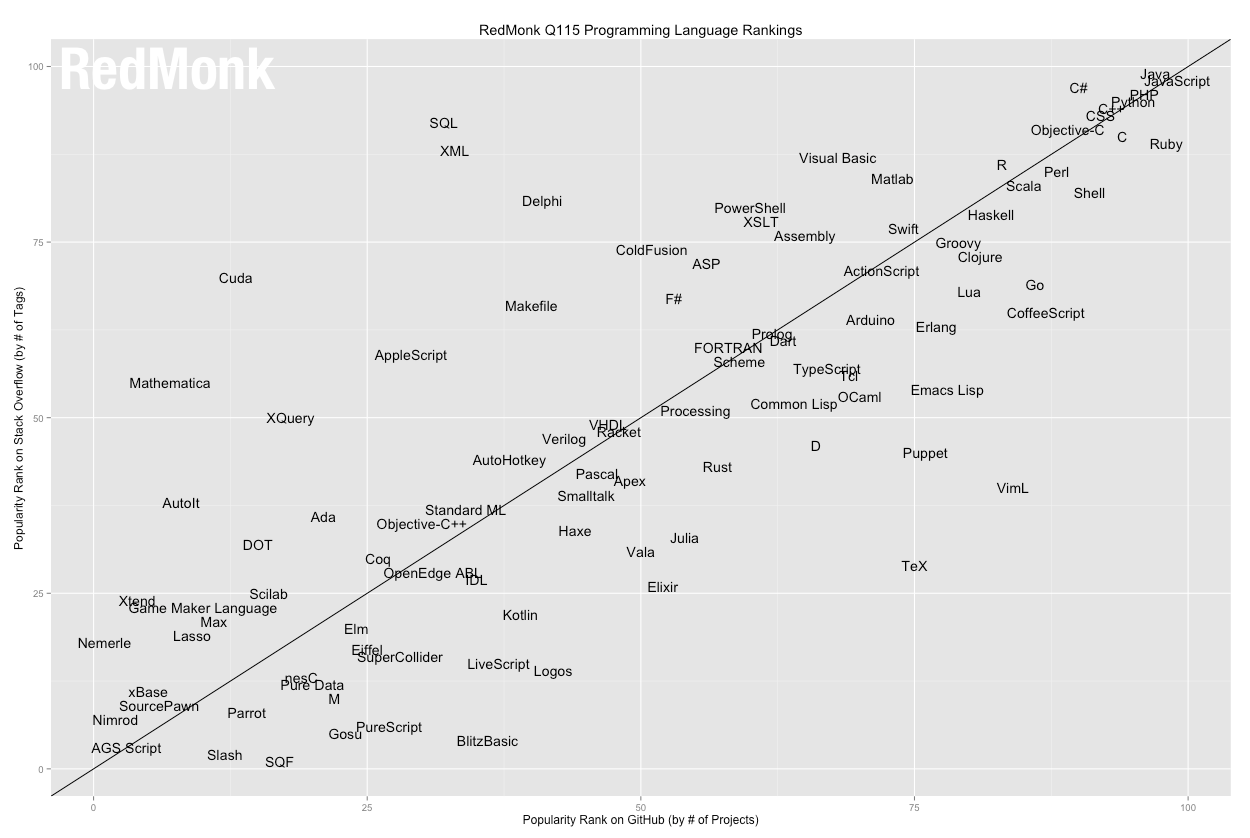
\includegraphics[width=1\textwidth]{img/grafico_redmonk}
	\caption{Ranking das liguagens de programação no Stack Overflow e Github}
\end{figure}


Ainda assim, para compor a interface do dado projeto, também ocorrerá o uso do líder JavaScript de forma intensa, provendo o elo com o as informações gerenciadas pelo PHP.


Entretanto, não seria inteligente desenvolver um sistema completo sem o auxílio de um framework. Dentre os frameworks disponíveis para PHP, hoje o destaque está com o Laravel, que se encontra no topo dentre os mais utilizados no momento. 


A WebHostFace, uma empresa de hospedagem, compilou várias estatísticas para criar um infográfico mostrando os frameworks PHP mais populares de 2015. Utilizando informações sobre os próprios clientes, o Google Trends, estatísticas de repositórios do GitHub e a pesquisa do SitePoint “Best PHP Frameworks 2015”, a WebHostFace elaborou o seguinte infográfico: 

\begin{figure}
	\label{fig:graficoWebhostface}
	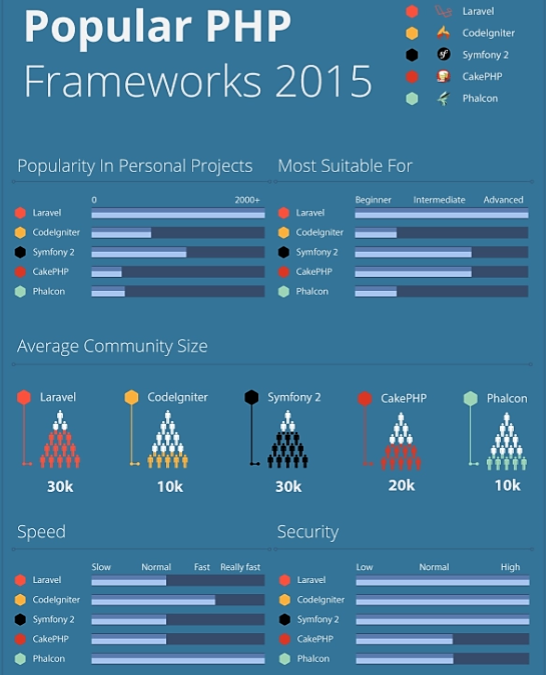
\includegraphics[width=1\textwidth]{img/infografico_webhostface}
	\caption{Infográfico da WebhostFace, exibindo a popularidade dos Frameworks PHP em 2015}
\end{figure}

Assim, tem-se a evidência que o Laravel em 2015 teve a maior popularidade em projetos pessoais e tem a maior comunidade entre os concorrentes, o que o torna uma boa escolha para a escrita de um software que será continuado por terceiros.


Para elaborar os recursos de interface e integrar ao back-end PHP do sistema, será adotado o já conhecido AngularJS, ferramenta sólida e conhecida no aspecto em questão. 


Dados coletados via Google Trends, que propõe comparações entre termos pesquisados, revela a popularidade do AngularJs diante de alguns dos principais concorrentes. O gráfico abaixo evidencia o cenário.


%Como mostra a Figura \ref{fig:graficoGoogleTrendsFerramentasFront}. 
\begin{figure}
	\label{fig:graficoGoogleTrendsFerramentasFront}
	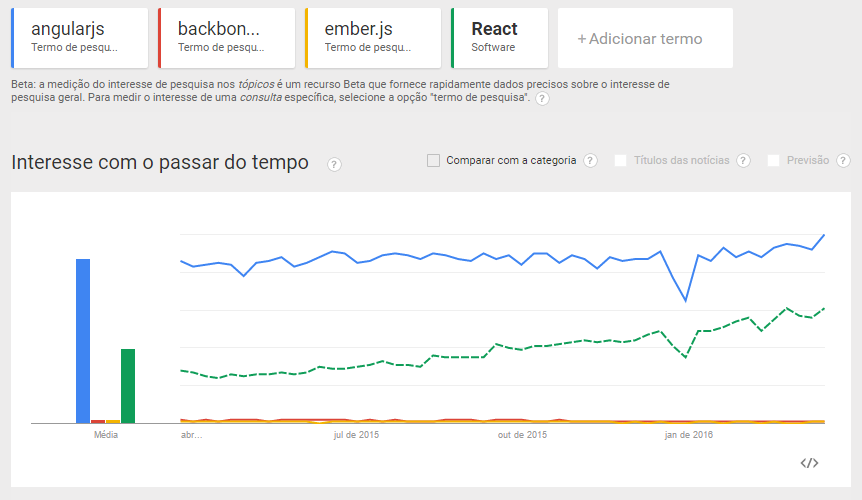
\includegraphics[width=1\textwidth]{img/grafico_ferramentas_front}
	\caption{Gráfico do Google Trends exibindo as pesquisas por ferramentas front-end}
\end{figure}


Junto ao Angular JS, será utilizada a agradável tendência de interface do Material Design da Google, que propõe layouts limpos e otimizados já conhecidos pelos usuários de smartphones Android. 


Para a elaboração da plataforma mobile do projeto, será utilizado o Ionic Framework, muito difundido e bastante pesquisado na área, o que fica evidenciado com o gráfico de pesquisbaixo, coletado via Google Trends buscando por frameworks de desenvolvimento híbrido mobile.


\begin{figure}
	\label{fig:graficoGoogleTrendsFerramentasHibridasMobile}
	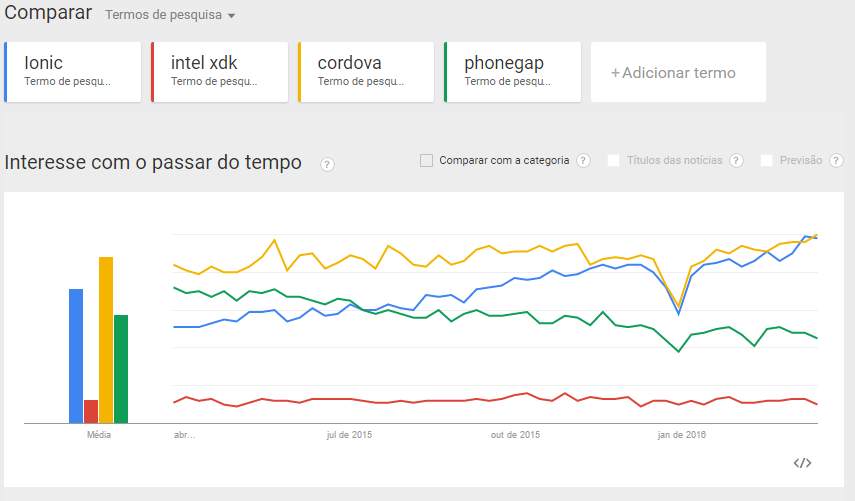
\includegraphics[width=1\textwidth]{img/grafico_ferramentas_hibridas_mobile}
	\caption{Gráfico do Google Trends exibindo as pesquisas por Frameworks híbridos mobile}
\end{figure}	

Para layout da interface mobile, também será aplicado a tendência do Material Design, a fim de propor uma harmonia entre o módulo web e mobile para os usuários


\section{Resultados Esperados}


Como fruto de um sistema para pós-graduação da UFBA, espera-se que os professores tenham mais recursos para integrar as atividades e também prover melhores condições para acompanhamento da vida acadêmica dos alunos em questão. Também, que os novos colaboradores que entrarem no processo tenham facilidade de compreender o fluxo do setor ao navegar pelo sistema proposto.


\section{Fora de Escopo}


Interação com os alunos devido às complicações para realizar a integração com o sistema empregado na UFBA, gerenciado pela XXXXXX, o que causaria uma inviabilidade no projeto devido à necessidade de entrega do produto ser mais forte que o tempo necessário para executar o processo de obtenção de acesso ao sistema legado para realizar a integração.


\section{Estrutura do Trabalho}


<breve resumo sobre os capítulos do TCC>
\chapter{Referencial Teórico}


Projetar o desenvolvimento de um software requer muito planejamento, pois as falhas iniciais podem custar bastante caro ou até mesmo inviabilizar a continuação de um projeto. Assim, a escolha da arquitetura ideal para a aplicabilidade é essencial na concepção de um produto de software. 
De todo o modo, sempre busca-se fazer mais com menos. Diante de tal filosofia, temos nesta seção, uma breve discussão sobre alguns elementos de projeto e arquitetura de software, a fim de contextualizar este trabalho de conclusão de curso.


% Ser direto no começo, focando no que realmente será discutido A seção \ref{sec:apps_mobile} 
 \section{Software como serviço}\label{sec:saas}


A definição de SaaS encontra-se muito bem elaborada em um dos trabalhos listados na literatura. Segundo La e Chun \citep{La2009Systematic}, o princípio da definição de Software como um Serviço (Sofware as a Service - SaaS) é um serviço complementar para aplicações da computação em nuvem (cloud computing). As duas áreas estão interligadas, no entanto, não se confundem, pois o SaaS deve ser entendido como um mecanismo de suporte às soluções existentes na cloud. Os SaaS existem justamente para maximizar o reuso de serviços repetidos e não centrais em uma aplicação remota.


Como propõe vantagens, software como servico é uma tendência forte, isso graças à evolução da web. Diversos fatores podem ser favoráveis para a adoção de um SaaS, como custo e manutenção dentre outros fatores aplicaveis a determinados contextos. Um trabalho recente realizado por Lechessa et al. \cite{LechesaSS11} apresenta uma pesquisa qualitativa sobre os fatores determinantes para adoção ou não de um SaaS voltado para ERP na África do Sul. Esses autores indicam que os principais fatores determinantes para adoção desse mecanismo de software são sua fluidez quanto à rede e a segurança. Esses fatores estão presentes na aplicação desenvolvida neste trabalho de conclusão de curso.
 

Devido ao fato de ter um serviço constantemente na nuvem, fica o questionamento sobre a segurança da informação manipulada. Sabe-se que a vulnerabilidade na web não é restrita ao SaaS, atingindo diversos âmbitos. O artigo de Rai et al. \cite{journals/corr/RaiSM13} orienta como o avanço da computação em nuvem não é um problema apenas para os serviços web do ponto de vista da segurança, pois muitos trabalhos na literatura mostram a área como mais um ponto de vulnerabilidade para diversos setores, a exemplo de infraestrutura. No mesmo artigo mencionado de Rai et al. \cite{journals/corr/RaiSM13}, também realizaram-se estudos exploratórios junto a empresas usuárias de serviços em computação em nuvem e consideram que a perspectiva de SaaS também pode fortalecer a segurança nas aplicações de cloud computing, pois o software de autenticação compartilhado por várias aplicações em nuvem, oferece uma melhor padronização e consequente facilidade de prevenção a erros de vulnerabilidade específicas de cada módulo da pesquisa. Esse ponto de vista é muito importante para qualquer trabalho de ponta na área de SaaS.


A arquitetura de armazenamento de dados de um Saas pode variar de acordo com a necessidade do contexto. O artigo recente de Huixin \cite{7586486}, exemplifica possíveis modelagens para utilizar. Tal abordagem pode ser com um banco de dados único, fazendo com que diferentes clientes compartilhem o mesmo banco, diferindo os dados através de controle de usuário, ou isolando os diferentes clientes através de bancos de dados exclusivos para cada um. Tal fator também pode ser combinado com a arquitetura da aplicação, caso ofereça aplicação única para todos os clientes ou aplicação compartilhada. Diante das possíveis abprdagens, a modelagem de dados do software pode ser decidida pela regra de negócio. Este trabalho optou por aplicação única e banco de dados compartilhado.


Devido ao diferente conceito de obtenção de software, tanto pela visão do cliente como pela visão do vendedor, é necessário tomar conhecimento dos diversos fatores que podem ser relevantes ao orçar um Saas. O recente trabalho de T. Kaur et al. \citep{6949281} orienta um modelo para compor o custo de um Saas. O custo total seria composto pelos fatores que dão suporte ao funcionamento do software. Tais fatores incluem infra-estrutura, configurabilidade, customização, parâmetros de QoS(Quality of service) como escalabilidade, disponibilidade, usabilidade, pontualidade e desempenho da resposta, portabilidade, custo total de propriedade e retorno do investimento. Esses fatores caracterizam o custo de forma eficaz, possibilitando ao fornecedor, prover um Serviço de acordo com a exigência do consumidor em vários pacotes de serviços.


\section{Reuso de software}\label{sec:reuso} %CRUISE BOOK CAPITULO 2


Para Peter Freeman, o reuso é a utilização de qualquer informação que um desenvolvedor pode necessitar no processo de criação de software (Ezran et al., 2002). Basili e Rombach definem reutilização de software como o uso de tudo o que está associado a um projeto de conhecimento (Basili e Rombach, 1991).
Assim, o objetivo da reutilização de software é reciclar o design, código e outros componentes de um produto de software e assim reduzir o custo, o tempo e melhorar a qualidade do produto.
Segundo Keswani et al. \cite{6783445}, o componente reutilizável de software pode ser qualquer parte de seu desenvolvimento, como um fragmento de código, design, casos de teste, ou até mesmo a especificação de requisitos de uma funcionalidade do software. 

O reuso de software pode ter impacto positivo em diversos aspectos do software, vejamos alguns, conforme apresentados no C.R.U.I.S.E Book:

\begin{itemize}

\item Qualidade: As correções de erro tornam-se úteis em todos os locais em que ocorreu, padronizando e facilitando a manutenção.

\item Produtividade: O ganho de produtividade é alcançado devido ao menor número de artefatos desenvolvido. Isso resulta em menos esforços de teste e também economiza análise e design, gerando economia em diversos escopos do projeto.

\item Confiabilidade: A utilização de componentes bem testados aumenta a
confiança no software. Além disso, a utilização de um mesmo componente em vários sistemas, aumenta a possibilidade de detecção de erros e reforça a confiança no componente.

\item Redução do Esforço: A reutilização de software proporciona uma redução do tempo de desenvolvimento, o que reduz o tempo necessário para o produto ser disponibilizado no mercado para trazer rentabilidade.

\item Trabalho redundante e tempo de desenvolvimento: Desenvolver um sistema do
zero significa desenvolvimento redundante de muitos componentes, como requisito
especificações, casos de uso, arquitetura, etc. Isso pode ser evitado quando estes estão disponíveis como componentes reutilizáveis e podem ser compartilhados, resultando em menos desenvolvimento, tempo e custo associado.

\item Documentação: Embora a documentação seja muito importante para a
manutenção de um sistema, muitas vezes é negligenciada. A reutilização de componentes software reduz a quantidade de documentação a ser escrita, entretanto depende da qualidade do que está escrito. Assim, apenas a estrutura do sistema e os novos artefatos desenvolvidos necessitam ser documentados.

\item Custo de manutenção: Menos defeitos e manutenções são esperados quando tem-se comprovada a qualidade dos componentes utilizados.

\item Tamanho da equipe: É comum entrar casos em que a equipe de desenvolvimento sofre sobrecarga. Entretanto, dobrar o tamanho da equipe de desenvolvimento não necessariamente duplica produtividade. Se muitos componentes podem ser reutilizados, é possível desenvolver com equipes menores, levando a melhores comunicações e aumento da produtividade.

\end{itemize}

Apesar dos benefícios da reutilização de software, a mesma não é amplamente praticado como imagina-se. Existem fatores que influenciam direta ou indiretamente na sua adoção. Esses fatores podem ser de aspecto gerencial, organizacional, econômico, conceitual ou técnico. Veremos a seguir alguns aspectos que podem gerar conflito com a cultura de reuso de software, segundo o C.R.U.I.S.E Book:
%(Sametinger, 1997). REVER

\begin{itemize}
	
\item Falta de apoio da gestão: Como a reutilização de software gera custos iniciais,
a medida pode não ser amplamente alcançada em uma organização sem o apoio de alto nível gestão. Os gestores têm de ser informados sobre os custos iniciais e serem convencidos sobre economias futuras.

\item Gerenciamento do Projeto: Gerenciar projetos tradicionais é uma tarefa árdua, principalmente, os que praticam a reutilização de software. Utilizando a técnica em larga escala, tem-se impacto sobre todo o ciclo de vida do software.

\item Estruturas organizacionais inadequadas: As estruturas organizacionais devem
considerar diferentes necessidades que surgem quando a reutilização em larga escala está sendo adotada. Por exemplo, uma equipe particionada pode ser alocada somente para desenvolver, manter e certificar componentes reutilizáveis de software.

\item Incentivos de gestão: É comum a falta de incentivo para deixar os desenvolvedores gastarem tempo elaborando reutilizáveis componentes do sistema. A produtividade é muitas vezes medida apenas no tempo necessário para concluir um projeto. Assim, fazer qualquer trabalho além disso, embora benéfico para a empresa como um todo, diminui o seu sucesso. Mesmo quando os componentes reutilizáveis são utilizados, os benefícios obtidos são uma pequena fração do que poderia ser alcançado caso houvesse reutilização explícita, planejada e organizada.

\item Dificuldade de encontrar software reutilizável: Para reutilizar os componentes, devem existir formas eficientes de busca. Além disso, é importante ter um repositório bem organizado contendo componentes com um eficiente meio de acesso.

\item Não reutilização do software encontrado. O acesso fácil ao software existente
não necessariamente aumentar a reutilização. Os componentes reutilizáveis devem ser cuidadosamente especificados, projetados, implementados e documentados, pois em alguns casos, modificar e adaptar o código  pode ser mais custoso que a programação da funcionalidade necessária a partir do zero.

\item Modificação: É muito difícil encontrar um componente que funcione
exatamente da mesma maneira que queremos. Desta forma, são necessárias modificações e devem existir formas de determinar os seus efeitos sobre o componente.


\end{itemize}


%Outra diretriz importante para a reutilização de software é reduzir o risco na criação de novos softwares. O risco tende a ser bastante reduzido se os componentes que estão sendo reutilizados têm as documentação, interfaces necessárias e devidamente testadas, fatores que contibruem para uma fácil integração.
%De acordo com Keswani et al. \citep{6783445}, para o reuso de software dar retornos apropriados, o processo deve ser sistemático e planejado. Qualquer organização que implemente a reutilização de software deve identificar os melhores métodos e estratégias de reutilização para obter a máxima produtividade. A reutilização de software ajuda a evitar software de engenharia a partir do zero, pois usa módulos de software existentes. A reutilização de software, embora seja uma tarefa difícil, especialmente para softwares antigos sem padrões de projeto, pode melhorar significativamente a produtividade e a qualidade de um produto de software. Embora a reutilização de software não seja um novo campo, ela pode dar grandes retornos em curto período de tempo.


\section{Modularização}\label{sec:modularizacao} %artigo de claudio pagina 222 introdução


%A modularidade vem desempenhando um papel predominante estágios emergentes das disciplinas de arquitetura de software [13]. Engenheiros de software consideram modularidade como princípio base na comparação entre arquiteturas alternativas  e arquitetura degeneração [9]. De fato, os engenheiros de software são incentivados a arquitecturas, baseando-se numa multiplicidade de mecanismos de modularidade disponíveis em: 
%(i) Linguagens de descrição de arquitetura (ADLs), como ACME [8], 
%(ii) catálogos de arquitetônicos [2, 13], e 
%(iii) conhecem bem princípios de alto nível, como interfaces de componentes estreitos, acoplamento arquitectónico reduzido e semelhantes.


Conforme é frisado no trabalho de Wickramaarachchi e Lai \citep{7062705}, o conceito de modularização na indústria de software tem uma longa história e tem sido utilizado para melhorar o processo de desenvolvimento de software em diferentes estágios. Os principais conceitos por trás da modularização do software foram introduzidos por pesquisadores pioneiros há quarenta anos, com uma notável contribuição feita por Melvin Conway e David Parnas, que tem representação notável na engenharia de software.


Modularizar um software é um bom padrão a ser adotado. Segundo Wickramaarachchi e Lai \citep{7062705}, a modularização é importante na identificação de dependências e reduz as dificuldades diante de uma possível necessidade de grandes alterações. De uma perspectiva da engenharia de software, uma modularização geralmente tem várias vantagens, tais como: tornar a complexidade do software mais gerenciável, facilitar o trabalho paralelo e tornar o software mais maleável para acomodar o futuro incerto que um software pode ter. O objetivo final da modularização do software é aumentar a produtividade ea qualidade do software. Tal conceito encontra-se bastante difundido e estái incorporado em linguagens de programação e ferramentas de software. O trabalho proposto favorece ao uso da modularização de um software e até mesmo pode ser considerado um módulo a ser acoplado a qualquer software, mediante a compatibilidade.


\section{Aplicações web}\label{sec:apps_web}


A popularidade da aplicação web aumentou exponencialmente na última década e todos os dias cresce o número de pessoas usuárias de aplicações web. E seguindo o padrão de desenvolvimento de software, Kumar et al. \citep{7813710} sugerem que para o desenvolvimento web, deve-se manter a prática efiacaz de produzir diagramas UML. A abordagem baseada na web oferece uma maneira fácil e eficaz para gerenciar e controlar o processo de desenvolvimento por meio de diagramas UML. Tal abordagem pode ser usada quando há uma exigência de lidar com mudanças muito rápidas e grandes em requisitos de forma muito eficaz em muito menos tempo, gerando assim um menor impacto. 


Para atender à fomentada demanda de aplicativos web, é necessário adotar métodos de desenvolvimentos que sejam ágeis, eficientes e de fácil manutenção. Yu Ping et al. \cite{1372143} propõem o uso do modelo MVC (Model, View e Controller) no atual desenvolvimento para softwares web. O modelo apresentado tornou-se um padrão popular e divide o software em camadas com propósito definido, tornando-o de mais fácil manutenção.


O Ajax (Asynchronous Javascript and XML) revolucionou a web. Conforme demonstrado no artigo de Yuping \citep{6845605}, ao usar a tecnologia Ajax, podemos enriquecer a experiência do usuário em aplicações baseadas em navegador de internet, e fornecer uma variedade de aplicações interativas para atender às necessidade de humanização das aplicações.
Os aplicativos Ajax em execução no navegador se comunicam com um servidor Web de forma assíncrona e atualizam apenas uma parte da página.



% %% RiSE Latex Template - version 0.5
%%
%% RiSE's latex template for thesis and dissertations
%% http://risetemplate.sourceforge.net
%%
%% (c) 2012 Yguaratã Cerqueira Cavalcanti (yguarata@gmail.com)
%%          Vinicius Cardoso Garcia (vinicius.garcia@gmail.com)
%%
%% This document was initially based on UFPEThesis template, from Paulo Gustavo
%% S. Fonseca.
%%
%% ACKNOWLEDGEMENTS
%%
%% We would like to thanks the RiSE's researchers community, the 
%% students from Federal University of Pernambuco, and other users that have
%% been contributing to this projects with comments and patches.
%%
%% GENERAL INSTRUCTIONS
%%
%% We strongly recommend you to compile your documents using pdflatex command.
%% It is also recommend use the texlipse plugin for Eclipse to edit your documents.
%%
%% Options for \documentclass command:
%%         * Idiom
%%           pt   - Portguese (default)
%%           en   - English
%%
%%         * Text type
%%           bsc  - B.Sc. Thesis
%%           msc  - M.Sc. Thesis (default)
%%           qual - PHD qualification (not tested yet)
%%           prop - PHD proposal (not tested yet)
%%           phd  - PHD thesis
%%
%%         * Media
%%           scr  - to eletronic version (PDF) / see the users guide
%%
%%         * Pagination
%%           oneside - unique face press
%%           twoside - two faces press
%%
%%		   * Line spacing
%%           singlespacing  - the same as using \linespread{1}
%%           onehalfspacing - the same as using \linespread{1.3}
%%           doublespacing  - the same as using \linespread{1.6}
%%
%% Reference commands. Use the following commands to make references in your
%% text:
%%          \figref  -- for Figure reference
%%          \tabref  -- for Table reference
%%          \eqnref  -- for equation reference
%%          \chapref -- for chapter reference
%%          \secref  -- for section reference
%%          \appref  -- for appendix reference
%%          \axiref  -- for axiom reference
%%          \conjref -- for conjecture reference
%%          \defref  -- for definition reference
%%          \lemref  -- for lemma reference
%%          \theoref -- for theorem reference
%%          \corref  -- for corollary reference
%%          \propref -- for proprosition reference
%%          \pgref   -- for page reference
%%
%%          Example: See \chapref{chap:introduction}. It will produce 
%%                   'See Chapter 1', in case of English language.

\documentclass[pt,twoside,onehalfspacing,bsc]{risethesis}

\usepackage[utf8]{inputenc}
\usepackage[brazilian]{babel}
\usepackage[T1]{fontenc}

%% Change the following pdf author attribute name to your name.
\usepackage[linkcolor=blue,citecolor=blue,urlcolor=blue,colorlinks,pdfpagelabels,pdftitle={Bruno Cabral's Bachelor Thesis},pdfauthor={Bruno Cabral}]{hyperref}

\address{SALVADOR}

\universitypt{Universidade Federal da Bahia}
\universityen{Federal University of Bahia}

\departmentpt{Depertamento de Ciência da Computação}
\departmenten{Computer Science Department}

\programpt{Programa Multiinstitucional de Pós-graduação em Ciência da Computação}
\programen{Graduate in Computer Science}

\majorfieldpt{Ciência da Computação}
\majorfielden{Computer Science}

\title{Sistema de apoio à Pós graduação - UFBA}
\date{Outubro/2016}

\author{Victor de Azevedo Nunes}
\adviser{Ivan do Carmo Machado}

\begin{document}

\frontmatter
\frontpage
\presentationpage

\begin{dedicatory}
Eu dedico esta dissertação...
%I dedicate this dissertation to my family, girlfriend, friends and
%professors who gave me all necessary support to get here.
\end{dedicatory}

\acknowledgements
Meus agradecimentos...

\begin{epigraph}[]{Edward V Berard}
Walking on water and developing software from a specification are easy if both are frozen
\end{epigraph}

\resumo
% Escreva seu resumo no arquivo resumo.tex
\input{resumo}

\abstract
% Write your abstract in a file called abstract.tex
\input{abstract}

% Summary (tables of contents)
\tableofcontents

% List of figures
\listoffigures

% List of tables
\listoftables

% List of acronyms
% Acronyms manual: http://linorg.usp.br/CTAN/macros/latex/contrib/acronym/acronym.pdf
\listofacronyms
\input{acronyms}

% List of listings
%\lstlistoflistings

\mainmatter

\include{chapters/intro}
\include{chapters/referencial_teorico}

% \include{chapters/introduction/main}
% \include{chapters/background/main}
% \include{chapters/proposed_solution/main}
% \include{chapters/experiment/main}
% \include{chapters/conclusion/main}

\bibliographystyle{natbib}
\addcontentsline{toc}{chapter}{\bibliographytocname}
\bibliography{references}

% Appendix
\clearpage
\addappheadtotoc
\appendix
\appendixpage
% \include{appendix/experiment-instruments}

\end{document}
% %% RiSE Latex Template - version 0.5
%%
%% RiSE's latex template for thesis and dissertations
%% http://risetemplate.sourceforge.net
%%
%% (c) 2012 Yguaratã Cerqueira Cavalcanti (yguarata@gmail.com)
%%          Vinicius Cardoso Garcia (vinicius.garcia@gmail.com)
%%
%% This document was initially based on UFPEThesis template, from Paulo Gustavo
%% S. Fonseca.
%%
%% ACKNOWLEDGEMENTS
%%
%% We would like to thanks the RiSE's researchers community, the 
%% students from Federal University of Pernambuco, and other users that have
%% been contributing to this projects with comments and patches.
%%
%% GENERAL INSTRUCTIONS
%%
%% We strongly recommend you to compile your documents using pdflatex command.
%% It is also recommend use the texlipse plugin for Eclipse to edit your documents.
%%
%% Options for \documentclass command:
%%         * Idiom
%%           pt   - Portguese (default)
%%           en   - English
%%
%%         * Text type
%%           bsc  - B.Sc. Thesis
%%           msc  - M.Sc. Thesis (default)
%%           qual - PHD qualification (not tested yet)
%%           prop - PHD proposal (not tested yet)
%%           phd  - PHD thesis
%%
%%         * Media
%%           scr  - to eletronic version (PDF) / see the users guide
%%
%%         * Pagination
%%           oneside - unique face press
%%           twoside - two faces press
%%
%%		   * Line spacing
%%           singlespacing  - the same as using \linespread{1}
%%           onehalfspacing - the same as using \linespread{1.3}
%%           doublespacing  - the same as using \linespread{1.6}
%%
%% Reference commands. Use the following commands to make references in your
%% text:
%%          \figref  -- for Figure reference
%%          \tabref  -- for Table reference
%%          \eqnref  -- for equation reference
%%          \chapref -- for chapter reference
%%          \secref  -- for section reference
%%          \appref  -- for appendix reference
%%          \axiref  -- for axiom reference
%%          \conjref -- for conjecture reference
%%          \defref  -- for definition reference
%%          \lemref  -- for lemma reference
%%          \theoref -- for theorem reference
%%          \corref  -- for corollary reference
%%          \propref -- for proprosition reference
%%          \pgref   -- for page reference
%%
%%          Example: See \chapref{chap:introduction}. It will produce 
%%                   'See Chapter 1', in case of English language.

\documentclass[pt,twoside,onehalfspacing,bsc]{risethesis}

\usepackage[utf8]{inputenc}
\usepackage[brazilian]{babel}
\usepackage[T1]{fontenc}

%% Change the following pdf author attribute name to your name.
\usepackage[linkcolor=blue,citecolor=blue,urlcolor=blue,colorlinks,pdfpagelabels,pdftitle={Bruno Cabral's Bachelor Thesis},pdfauthor={Bruno Cabral}]{hyperref}

\address{SALVADOR}

\universitypt{Universidade Federal da Bahia}
\universityen{Federal University of Bahia}

\departmentpt{Depertamento de Ciência da Computação}
\departmenten{Computer Science Department}

\programpt{Programa Multiinstitucional de Pós-graduação em Ciência da Computação}
\programen{Graduate in Computer Science}

\majorfieldpt{Ciência da Computação}
\majorfielden{Computer Science}

\title{Sistema de apoio à Pós graduação - UFBA}
\date{Outubro/2016}

\author{Victor de Azevedo Nunes}
\adviser{Ivan do Carmo Machado}

\begin{document}

\frontmatter
\frontpage
\presentationpage

\begin{dedicatory}
Eu dedico esta dissertação...
%I dedicate this dissertation to my family, girlfriend, friends and
%professors who gave me all necessary support to get here.
\end{dedicatory}

\acknowledgements
Meus agradecimentos...

\begin{epigraph}[]{Edward V Berard}
Walking on water and developing software from a specification are easy if both are frozen
\end{epigraph}

\resumo
% Escreva seu resumo no arquivo resumo.tex
\input{resumo}

\abstract
% Write your abstract in a file called abstract.tex
\input{abstract}

% Summary (tables of contents)
\tableofcontents

% List of figures
\listoffigures

% List of tables
\listoftables

% List of acronyms
% Acronyms manual: http://linorg.usp.br/CTAN/macros/latex/contrib/acronym/acronym.pdf
\listofacronyms
\input{acronyms}

% List of listings
%\lstlistoflistings

\mainmatter

\include{chapters/intro}
\include{chapters/referencial_teorico}

% \include{chapters/introduction/main}
% \include{chapters/background/main}
% \include{chapters/proposed_solution/main}
% \include{chapters/experiment/main}
% \include{chapters/conclusion/main}

\bibliographystyle{natbib}
\addcontentsline{toc}{chapter}{\bibliographytocname}
\bibliography{references}

% Appendix
\clearpage
\addappheadtotoc
\appendix
\appendixpage
% \include{appendix/experiment-instruments}

\end{document}
% %% RiSE Latex Template - version 0.5
%%
%% RiSE's latex template for thesis and dissertations
%% http://risetemplate.sourceforge.net
%%
%% (c) 2012 Yguaratã Cerqueira Cavalcanti (yguarata@gmail.com)
%%          Vinicius Cardoso Garcia (vinicius.garcia@gmail.com)
%%
%% This document was initially based on UFPEThesis template, from Paulo Gustavo
%% S. Fonseca.
%%
%% ACKNOWLEDGEMENTS
%%
%% We would like to thanks the RiSE's researchers community, the 
%% students from Federal University of Pernambuco, and other users that have
%% been contributing to this projects with comments and patches.
%%
%% GENERAL INSTRUCTIONS
%%
%% We strongly recommend you to compile your documents using pdflatex command.
%% It is also recommend use the texlipse plugin for Eclipse to edit your documents.
%%
%% Options for \documentclass command:
%%         * Idiom
%%           pt   - Portguese (default)
%%           en   - English
%%
%%         * Text type
%%           bsc  - B.Sc. Thesis
%%           msc  - M.Sc. Thesis (default)
%%           qual - PHD qualification (not tested yet)
%%           prop - PHD proposal (not tested yet)
%%           phd  - PHD thesis
%%
%%         * Media
%%           scr  - to eletronic version (PDF) / see the users guide
%%
%%         * Pagination
%%           oneside - unique face press
%%           twoside - two faces press
%%
%%		   * Line spacing
%%           singlespacing  - the same as using \linespread{1}
%%           onehalfspacing - the same as using \linespread{1.3}
%%           doublespacing  - the same as using \linespread{1.6}
%%
%% Reference commands. Use the following commands to make references in your
%% text:
%%          \figref  -- for Figure reference
%%          \tabref  -- for Table reference
%%          \eqnref  -- for equation reference
%%          \chapref -- for chapter reference
%%          \secref  -- for section reference
%%          \appref  -- for appendix reference
%%          \axiref  -- for axiom reference
%%          \conjref -- for conjecture reference
%%          \defref  -- for definition reference
%%          \lemref  -- for lemma reference
%%          \theoref -- for theorem reference
%%          \corref  -- for corollary reference
%%          \propref -- for proprosition reference
%%          \pgref   -- for page reference
%%
%%          Example: See \chapref{chap:introduction}. It will produce 
%%                   'See Chapter 1', in case of English language.

\documentclass[pt,twoside,onehalfspacing,bsc]{risethesis}

\usepackage[utf8]{inputenc}
\usepackage[brazilian]{babel}
\usepackage[T1]{fontenc}

%% Change the following pdf author attribute name to your name.
\usepackage[linkcolor=blue,citecolor=blue,urlcolor=blue,colorlinks,pdfpagelabels,pdftitle={Bruno Cabral's Bachelor Thesis},pdfauthor={Bruno Cabral}]{hyperref}

\address{SALVADOR}

\universitypt{Universidade Federal da Bahia}
\universityen{Federal University of Bahia}

\departmentpt{Depertamento de Ciência da Computação}
\departmenten{Computer Science Department}

\programpt{Programa Multiinstitucional de Pós-graduação em Ciência da Computação}
\programen{Graduate in Computer Science}

\majorfieldpt{Ciência da Computação}
\majorfielden{Computer Science}

\title{Sistema de apoio à Pós graduação - UFBA}
\date{Outubro/2016}

\author{Victor de Azevedo Nunes}
\adviser{Ivan do Carmo Machado}

\begin{document}

\frontmatter
\frontpage
\presentationpage

\begin{dedicatory}
Eu dedico esta dissertação...
%I dedicate this dissertation to my family, girlfriend, friends and
%professors who gave me all necessary support to get here.
\end{dedicatory}

\acknowledgements
Meus agradecimentos...

\begin{epigraph}[]{Edward V Berard}
Walking on water and developing software from a specification are easy if both are frozen
\end{epigraph}

\resumo
% Escreva seu resumo no arquivo resumo.tex
\input{resumo}

\abstract
% Write your abstract in a file called abstract.tex
\input{abstract}

% Summary (tables of contents)
\tableofcontents

% List of figures
\listoffigures

% List of tables
\listoftables

% List of acronyms
% Acronyms manual: http://linorg.usp.br/CTAN/macros/latex/contrib/acronym/acronym.pdf
\listofacronyms
\input{acronyms}

% List of listings
%\lstlistoflistings

\mainmatter

\include{chapters/intro}
\include{chapters/referencial_teorico}

% \include{chapters/introduction/main}
% \include{chapters/background/main}
% \include{chapters/proposed_solution/main}
% \include{chapters/experiment/main}
% \include{chapters/conclusion/main}

\bibliographystyle{natbib}
\addcontentsline{toc}{chapter}{\bibliographytocname}
\bibliography{references}

% Appendix
\clearpage
\addappheadtotoc
\appendix
\appendixpage
% \include{appendix/experiment-instruments}

\end{document}
% %% RiSE Latex Template - version 0.5
%%
%% RiSE's latex template for thesis and dissertations
%% http://risetemplate.sourceforge.net
%%
%% (c) 2012 Yguaratã Cerqueira Cavalcanti (yguarata@gmail.com)
%%          Vinicius Cardoso Garcia (vinicius.garcia@gmail.com)
%%
%% This document was initially based on UFPEThesis template, from Paulo Gustavo
%% S. Fonseca.
%%
%% ACKNOWLEDGEMENTS
%%
%% We would like to thanks the RiSE's researchers community, the 
%% students from Federal University of Pernambuco, and other users that have
%% been contributing to this projects with comments and patches.
%%
%% GENERAL INSTRUCTIONS
%%
%% We strongly recommend you to compile your documents using pdflatex command.
%% It is also recommend use the texlipse plugin for Eclipse to edit your documents.
%%
%% Options for \documentclass command:
%%         * Idiom
%%           pt   - Portguese (default)
%%           en   - English
%%
%%         * Text type
%%           bsc  - B.Sc. Thesis
%%           msc  - M.Sc. Thesis (default)
%%           qual - PHD qualification (not tested yet)
%%           prop - PHD proposal (not tested yet)
%%           phd  - PHD thesis
%%
%%         * Media
%%           scr  - to eletronic version (PDF) / see the users guide
%%
%%         * Pagination
%%           oneside - unique face press
%%           twoside - two faces press
%%
%%		   * Line spacing
%%           singlespacing  - the same as using \linespread{1}
%%           onehalfspacing - the same as using \linespread{1.3}
%%           doublespacing  - the same as using \linespread{1.6}
%%
%% Reference commands. Use the following commands to make references in your
%% text:
%%          \figref  -- for Figure reference
%%          \tabref  -- for Table reference
%%          \eqnref  -- for equation reference
%%          \chapref -- for chapter reference
%%          \secref  -- for section reference
%%          \appref  -- for appendix reference
%%          \axiref  -- for axiom reference
%%          \conjref -- for conjecture reference
%%          \defref  -- for definition reference
%%          \lemref  -- for lemma reference
%%          \theoref -- for theorem reference
%%          \corref  -- for corollary reference
%%          \propref -- for proprosition reference
%%          \pgref   -- for page reference
%%
%%          Example: See \chapref{chap:introduction}. It will produce 
%%                   'See Chapter 1', in case of English language.

\documentclass[pt,twoside,onehalfspacing,bsc]{risethesis}

\usepackage[utf8]{inputenc}
\usepackage[brazilian]{babel}
\usepackage[T1]{fontenc}

%% Change the following pdf author attribute name to your name.
\usepackage[linkcolor=blue,citecolor=blue,urlcolor=blue,colorlinks,pdfpagelabels,pdftitle={Bruno Cabral's Bachelor Thesis},pdfauthor={Bruno Cabral}]{hyperref}

\address{SALVADOR}

\universitypt{Universidade Federal da Bahia}
\universityen{Federal University of Bahia}

\departmentpt{Depertamento de Ciência da Computação}
\departmenten{Computer Science Department}

\programpt{Programa Multiinstitucional de Pós-graduação em Ciência da Computação}
\programen{Graduate in Computer Science}

\majorfieldpt{Ciência da Computação}
\majorfielden{Computer Science}

\title{Sistema de apoio à Pós graduação - UFBA}
\date{Outubro/2016}

\author{Victor de Azevedo Nunes}
\adviser{Ivan do Carmo Machado}

\begin{document}

\frontmatter
\frontpage
\presentationpage

\begin{dedicatory}
Eu dedico esta dissertação...
%I dedicate this dissertation to my family, girlfriend, friends and
%professors who gave me all necessary support to get here.
\end{dedicatory}

\acknowledgements
Meus agradecimentos...

\begin{epigraph}[]{Edward V Berard}
Walking on water and developing software from a specification are easy if both are frozen
\end{epigraph}

\resumo
% Escreva seu resumo no arquivo resumo.tex
\input{resumo}

\abstract
% Write your abstract in a file called abstract.tex
\input{abstract}

% Summary (tables of contents)
\tableofcontents

% List of figures
\listoffigures

% List of tables
\listoftables

% List of acronyms
% Acronyms manual: http://linorg.usp.br/CTAN/macros/latex/contrib/acronym/acronym.pdf
\listofacronyms
\input{acronyms}

% List of listings
%\lstlistoflistings

\mainmatter

\include{chapters/intro}
\include{chapters/referencial_teorico}

% \include{chapters/introduction/main}
% \include{chapters/background/main}
% \include{chapters/proposed_solution/main}
% \include{chapters/experiment/main}
% \include{chapters/conclusion/main}

\bibliographystyle{natbib}
\addcontentsline{toc}{chapter}{\bibliographytocname}
\bibliography{references}

% Appendix
\clearpage
\addappheadtotoc
\appendix
\appendixpage
% \include{appendix/experiment-instruments}

\end{document}
% %% RiSE Latex Template - version 0.5
%%
%% RiSE's latex template for thesis and dissertations
%% http://risetemplate.sourceforge.net
%%
%% (c) 2012 Yguaratã Cerqueira Cavalcanti (yguarata@gmail.com)
%%          Vinicius Cardoso Garcia (vinicius.garcia@gmail.com)
%%
%% This document was initially based on UFPEThesis template, from Paulo Gustavo
%% S. Fonseca.
%%
%% ACKNOWLEDGEMENTS
%%
%% We would like to thanks the RiSE's researchers community, the 
%% students from Federal University of Pernambuco, and other users that have
%% been contributing to this projects with comments and patches.
%%
%% GENERAL INSTRUCTIONS
%%
%% We strongly recommend you to compile your documents using pdflatex command.
%% It is also recommend use the texlipse plugin for Eclipse to edit your documents.
%%
%% Options for \documentclass command:
%%         * Idiom
%%           pt   - Portguese (default)
%%           en   - English
%%
%%         * Text type
%%           bsc  - B.Sc. Thesis
%%           msc  - M.Sc. Thesis (default)
%%           qual - PHD qualification (not tested yet)
%%           prop - PHD proposal (not tested yet)
%%           phd  - PHD thesis
%%
%%         * Media
%%           scr  - to eletronic version (PDF) / see the users guide
%%
%%         * Pagination
%%           oneside - unique face press
%%           twoside - two faces press
%%
%%		   * Line spacing
%%           singlespacing  - the same as using \linespread{1}
%%           onehalfspacing - the same as using \linespread{1.3}
%%           doublespacing  - the same as using \linespread{1.6}
%%
%% Reference commands. Use the following commands to make references in your
%% text:
%%          \figref  -- for Figure reference
%%          \tabref  -- for Table reference
%%          \eqnref  -- for equation reference
%%          \chapref -- for chapter reference
%%          \secref  -- for section reference
%%          \appref  -- for appendix reference
%%          \axiref  -- for axiom reference
%%          \conjref -- for conjecture reference
%%          \defref  -- for definition reference
%%          \lemref  -- for lemma reference
%%          \theoref -- for theorem reference
%%          \corref  -- for corollary reference
%%          \propref -- for proprosition reference
%%          \pgref   -- for page reference
%%
%%          Example: See \chapref{chap:introduction}. It will produce 
%%                   'See Chapter 1', in case of English language.

\documentclass[pt,twoside,onehalfspacing,bsc]{risethesis}

\usepackage[utf8]{inputenc}
\usepackage[brazilian]{babel}
\usepackage[T1]{fontenc}

%% Change the following pdf author attribute name to your name.
\usepackage[linkcolor=blue,citecolor=blue,urlcolor=blue,colorlinks,pdfpagelabels,pdftitle={Bruno Cabral's Bachelor Thesis},pdfauthor={Bruno Cabral}]{hyperref}

\address{SALVADOR}

\universitypt{Universidade Federal da Bahia}
\universityen{Federal University of Bahia}

\departmentpt{Depertamento de Ciência da Computação}
\departmenten{Computer Science Department}

\programpt{Programa Multiinstitucional de Pós-graduação em Ciência da Computação}
\programen{Graduate in Computer Science}

\majorfieldpt{Ciência da Computação}
\majorfielden{Computer Science}

\title{Sistema de apoio à Pós graduação - UFBA}
\date{Outubro/2016}

\author{Victor de Azevedo Nunes}
\adviser{Ivan do Carmo Machado}

\begin{document}

\frontmatter
\frontpage
\presentationpage

\begin{dedicatory}
Eu dedico esta dissertação...
%I dedicate this dissertation to my family, girlfriend, friends and
%professors who gave me all necessary support to get here.
\end{dedicatory}

\acknowledgements
Meus agradecimentos...

\begin{epigraph}[]{Edward V Berard}
Walking on water and developing software from a specification are easy if both are frozen
\end{epigraph}

\resumo
% Escreva seu resumo no arquivo resumo.tex
\input{resumo}

\abstract
% Write your abstract in a file called abstract.tex
\input{abstract}

% Summary (tables of contents)
\tableofcontents

% List of figures
\listoffigures

% List of tables
\listoftables

% List of acronyms
% Acronyms manual: http://linorg.usp.br/CTAN/macros/latex/contrib/acronym/acronym.pdf
\listofacronyms
\input{acronyms}

% List of listings
%\lstlistoflistings

\mainmatter

\include{chapters/intro}
\include{chapters/referencial_teorico}

% \include{chapters/introduction/main}
% \include{chapters/background/main}
% \include{chapters/proposed_solution/main}
% \include{chapters/experiment/main}
% \include{chapters/conclusion/main}

\bibliographystyle{natbib}
\addcontentsline{toc}{chapter}{\bibliographytocname}
\bibliography{references}

% Appendix
\clearpage
\addappheadtotoc
\appendix
\appendixpage
% \include{appendix/experiment-instruments}

\end{document}

\bibliographystyle{natbib}
\addcontentsline{toc}{chapter}{\bibliographytocname}
\bibliography{references}

% Appendix
\clearpage
\addappheadtotoc
\appendix
\appendixpage
% \include{appendix/experiment-instruments}

\end{document}
% %% RiSE Latex Template - version 0.5
%%
%% RiSE's latex template for thesis and dissertations
%% http://risetemplate.sourceforge.net
%%
%% (c) 2012 Yguaratã Cerqueira Cavalcanti (yguarata@gmail.com)
%%          Vinicius Cardoso Garcia (vinicius.garcia@gmail.com)
%%
%% This document was initially based on UFPEThesis template, from Paulo Gustavo
%% S. Fonseca.
%%
%% ACKNOWLEDGEMENTS
%%
%% We would like to thanks the RiSE's researchers community, the 
%% students from Federal University of Pernambuco, and other users that have
%% been contributing to this projects with comments and patches.
%%
%% GENERAL INSTRUCTIONS
%%
%% We strongly recommend you to compile your documents using pdflatex command.
%% It is also recommend use the texlipse plugin for Eclipse to edit your documents.
%%
%% Options for \documentclass command:
%%         * Idiom
%%           pt   - Portguese (default)
%%           en   - English
%%
%%         * Text type
%%           bsc  - B.Sc. Thesis
%%           msc  - M.Sc. Thesis (default)
%%           qual - PHD qualification (not tested yet)
%%           prop - PHD proposal (not tested yet)
%%           phd  - PHD thesis
%%
%%         * Media
%%           scr  - to eletronic version (PDF) / see the users guide
%%
%%         * Pagination
%%           oneside - unique face press
%%           twoside - two faces press
%%
%%		   * Line spacing
%%           singlespacing  - the same as using \linespread{1}
%%           onehalfspacing - the same as using \linespread{1.3}
%%           doublespacing  - the same as using \linespread{1.6}
%%
%% Reference commands. Use the following commands to make references in your
%% text:
%%          \figref  -- for Figure reference
%%          \tabref  -- for Table reference
%%          \eqnref  -- for equation reference
%%          \chapref -- for chapter reference
%%          \secref  -- for section reference
%%          \appref  -- for appendix reference
%%          \axiref  -- for axiom reference
%%          \conjref -- for conjecture reference
%%          \defref  -- for definition reference
%%          \lemref  -- for lemma reference
%%          \theoref -- for theorem reference
%%          \corref  -- for corollary reference
%%          \propref -- for proprosition reference
%%          \pgref   -- for page reference
%%
%%          Example: See \chapref{chap:introduction}. It will produce 
%%                   'See Chapter 1', in case of English language.

\documentclass[pt,twoside,onehalfspacing,bsc]{risethesis}

\usepackage[utf8]{inputenc}
\usepackage[brazilian]{babel}
\usepackage[T1]{fontenc}

%% Change the following pdf author attribute name to your name.
\usepackage[linkcolor=blue,citecolor=blue,urlcolor=blue,colorlinks,pdfpagelabels,pdftitle={Bruno Cabral's Bachelor Thesis},pdfauthor={Bruno Cabral}]{hyperref}

\address{SALVADOR}

\universitypt{Universidade Federal da Bahia}
\universityen{Federal University of Bahia}

\departmentpt{Depertamento de Ciência da Computação}
\departmenten{Computer Science Department}

\programpt{Programa Multiinstitucional de Pós-graduação em Ciência da Computação}
\programen{Graduate in Computer Science}

\majorfieldpt{Ciência da Computação}
\majorfielden{Computer Science}

\title{Sistema de apoio à Pós graduação - UFBA}
\date{Outubro/2016}

\author{Victor de Azevedo Nunes}
\adviser{Ivan do Carmo Machado}

\begin{document}

\frontmatter
\frontpage
\presentationpage

\begin{dedicatory}
Eu dedico esta dissertação...
%I dedicate this dissertation to my family, girlfriend, friends and
%professors who gave me all necessary support to get here.
\end{dedicatory}

\acknowledgements
Meus agradecimentos...

\begin{epigraph}[]{Edward V Berard}
Walking on water and developing software from a specification are easy if both are frozen
\end{epigraph}

\resumo
% Escreva seu resumo no arquivo resumo.tex
Meu resumo

\begin{keywords}
palavras chave

\end{keywords}

\abstract
% Write your abstract in a file called abstract.tex
My abstract...

\begin{keywords}
key words...
\end{keywords}

% Summary (tables of contents)
\tableofcontents

% List of figures
\listoffigures

% List of tables
\listoftables

% List of acronyms
% Acronyms manual: http://linorg.usp.br/CTAN/macros/latex/contrib/acronym/acronym.pdf
\listofacronyms
\begin{acronym}[ACRONYM] 
% Change the word ACRONYM above to change the acronym column width.
% The column width is equals to the width of the word that you put.
% Read the manual about acronym package for more examples:
%   http://linorg.usp.br/CTAN/macros/latex/contrib/acronym/acronym.pdf

\acro{SPA}{Single Page Application}
\acro{JSON}{Javascript Object Notation}
\acro{PHP}{PHP: Hypertext Preprocessor}
\acro{SaaS}{Software as a Service}
\acro{ERP}{Enterprise Resource Planning}
\acro{QoS}{Quality of Service}
\acro{UML}{Unified Modeling Language}
\acro{MVC}{Model-View-Controller}
\acro{Ajax}{Asynchronous Javascript and XML}
\acro{HTML}{HyperText Markup Language}
\acro{CSS}{Cascading Style Sheets}
\acro{API}{Application Programming Interface}
\acro{DOM}{Document Object Model}
\acro{BPMN}{Business Process Model and Notation}
\acro{REST}{Representational State Transfer}

\end{acronym}

% List of listings
%\lstlistoflistings

\mainmatter

\chapter{Introdução}

\section{Motivação}

Organizar os procedimentos de um processo sempre nos traz vantagens. Apesar de no processo de implantação de um sistema, o mesmo burocratizar o processo, com o tempo temos o retorno da dedicação para a inserção dos dados. Com um certo volume de dados, é possível estruturar informações que num processo manual são difíceis de serem enxergadas. Assim, é possível depender menos das pessoas que organizam o processo, pois o legado de informações não estará mais somente na mente de alguns, mas sim documentado nos dados do sistema.

Além de colaborar na organização, também haverá uma grande colaboração no tempo gasto na gestão. Lidar com muitos papéis e confiar na mente humana para guardar informações, não é uma alternativa muito segura devido ao fato que as pessoas sempre estão sujeitas a sair do processo e levar contigo a experiência obtida. Experiência essa que faz com que os procedimentos sejam executados de forma mais eficiente. Entretanto, com um sistema inteligente, é possível auxiliar e tornar mais ágil a execução das tarefas.


\section{Problema}


De acordo com funcionários ligados ao o setor de pós graduação da UFBA, entrevistados a fim de um maior entendimento do cenário, apesar das semelhanças estruturais, a pós graduação gerida de forma diferencia da graduação. FULANO afirma que devido ao fato de não ter a mesma visibilidade, não tem acesso aos mesmos recursos de gestão acadêmica da graduação. O professores não executam somente atividades dentro da sala de aula, também tem diversas outras ocupações no setor. E muitos procedimentos realizados extra classe ainda se encontram sendo realizados de forma manual, estando mais vulnerável ao erro ou até mesmo à violação do processo. Também ocorre um grande desperdício de tempo pelos professores e gestores da área, devido ao diversos processos ainda realizados de forma manual, sem a devida documentação. Segundo FULANO, também entrevistado, esse tempo perdido implica numa redução da eficiência na sala de aula, pois o professor acaba por ter menos tempo disponível para o planejamento das atividades, o que gera impactos negativos aos alunos.


\section{Objetivos} %<o que deve ser feito/entregue>


Devido aos muitos processos sendo resolvidos de forma manual, propõe-se com solução um sistema moderno, arquitetado para ter funcionamento na web e com um módulo mobile, a fim de fornecer informações de forma rápida e eficiente para os professores através de notificações, já que o acesso à internet móvel é comum entre os possíveis usuários do sistema em questão.
O principal requisito para o sistema seria dispor recursos para reduzir o tempo desperdiçado pelos professores durante as atividades extra classe.


\section{Metodologia} %<como será feito | como resolver o problema apontado inicialmente>


%<analise de literatura | design | implementação | validação>
Baseando-se nas tecnologias gratuitas em alta no cenário atual do desenvolvimento web, dispomos de algumas opções eficientes para a implementação da solução. Dentre as possibilidades, considerando a facilidade para futura manutenção e continuidade do projeto, tende-se a optar por uma tecnologia popular. Como linguagem de programação, adota-se o PHP. A escolha é fundamentada de acordo com a pesquisa da RedMonk de 2015, que evidencia o uso das linguagens de programação de acordo com as discussões no StackOverflow e repositórios no GitHub. É possível constatar a popularidade do PHP no cenário atual com o gráfico da pesquisa citada, na qual o PHP é apresentado na terceira colocação, apenas atrás do lider JavaScript e do segundo colocado, o Java.

\begin{figure}
	\label{fig:graficoRedmonk}
	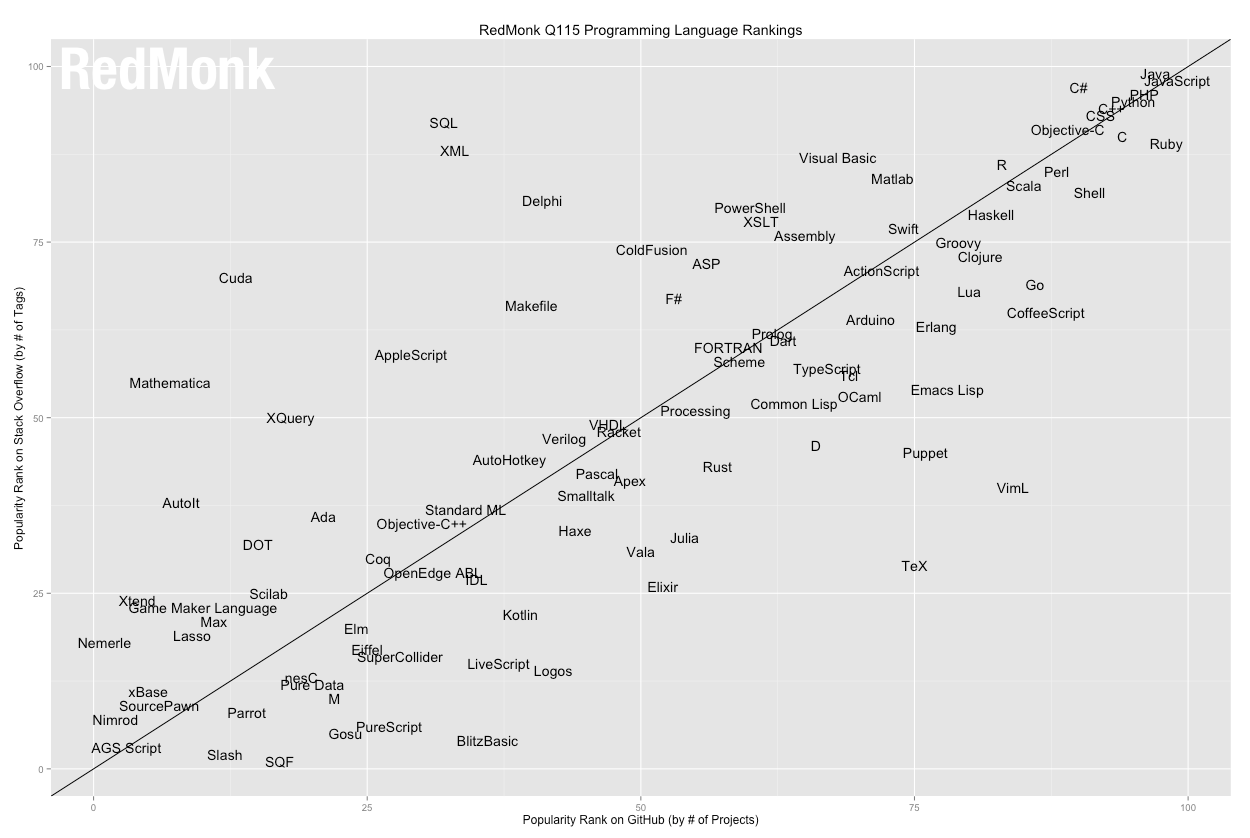
\includegraphics[width=1\textwidth]{img/grafico_redmonk}
	\caption{Ranking das liguagens de programação no Stack Overflow e Github}
\end{figure}


Ainda assim, para compor a interface do dado projeto, também ocorrerá o uso do líder JavaScript de forma intensa, provendo o elo com o as informações gerenciadas pelo PHP.


Entretanto, não seria inteligente desenvolver um sistema completo sem o auxílio de um framework. Dentre os frameworks disponíveis para PHP, hoje o destaque está com o Laravel, que se encontra no topo dentre os mais utilizados no momento. 


A WebHostFace, uma empresa de hospedagem, compilou várias estatísticas para criar um infográfico mostrando os frameworks PHP mais populares de 2015. Utilizando informações sobre os próprios clientes, o Google Trends, estatísticas de repositórios do GitHub e a pesquisa do SitePoint “Best PHP Frameworks 2015”, a WebHostFace elaborou o seguinte infográfico: 

\begin{figure}
	\label{fig:graficoWebhostface}
	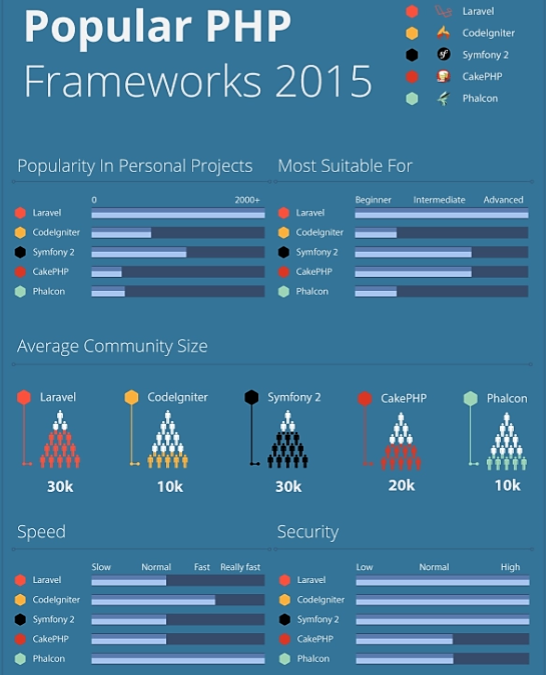
\includegraphics[width=1\textwidth]{img/infografico_webhostface}
	\caption{Infográfico da WebhostFace, exibindo a popularidade dos Frameworks PHP em 2015}
\end{figure}

Assim, tem-se a evidência que o Laravel em 2015 teve a maior popularidade em projetos pessoais e tem a maior comunidade entre os concorrentes, o que o torna uma boa escolha para a escrita de um software que será continuado por terceiros.


Para elaborar os recursos de interface e integrar ao back-end PHP do sistema, será adotado o já conhecido AngularJS, ferramenta sólida e conhecida no aspecto em questão. 


Dados coletados via Google Trends, que propõe comparações entre termos pesquisados, revela a popularidade do AngularJs diante de alguns dos principais concorrentes. O gráfico abaixo evidencia o cenário.


%Como mostra a Figura \ref{fig:graficoGoogleTrendsFerramentasFront}. 
\begin{figure}
	\label{fig:graficoGoogleTrendsFerramentasFront}
	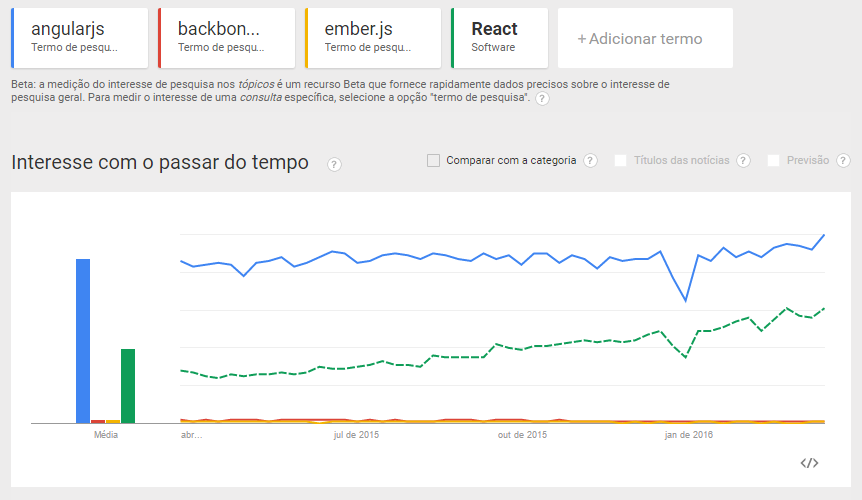
\includegraphics[width=1\textwidth]{img/grafico_ferramentas_front}
	\caption{Gráfico do Google Trends exibindo as pesquisas por ferramentas front-end}
\end{figure}


Junto ao Angular JS, será utilizada a agradável tendência de interface do Material Design da Google, que propõe layouts limpos e otimizados já conhecidos pelos usuários de smartphones Android. 


Para a elaboração da plataforma mobile do projeto, será utilizado o Ionic Framework, muito difundido e bastante pesquisado na área, o que fica evidenciado com o gráfico de pesquisbaixo, coletado via Google Trends buscando por frameworks de desenvolvimento híbrido mobile.


\begin{figure}
	\label{fig:graficoGoogleTrendsFerramentasHibridasMobile}
	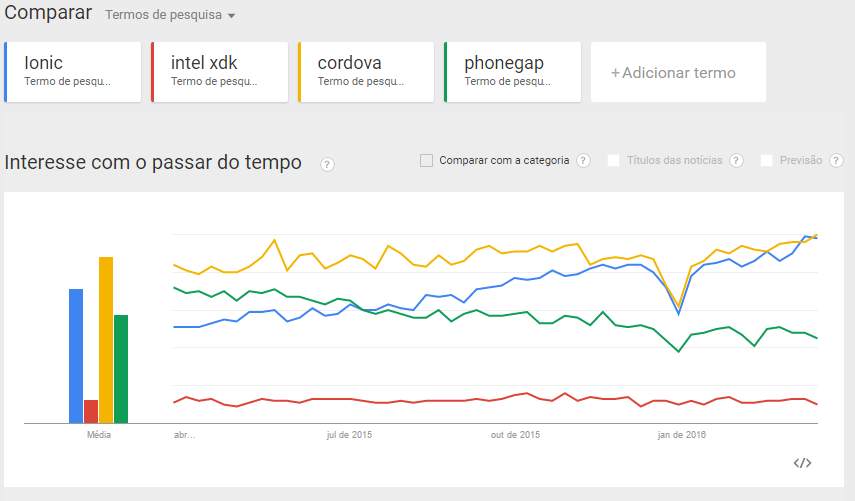
\includegraphics[width=1\textwidth]{img/grafico_ferramentas_hibridas_mobile}
	\caption{Gráfico do Google Trends exibindo as pesquisas por Frameworks híbridos mobile}
\end{figure}	

Para layout da interface mobile, também será aplicado a tendência do Material Design, a fim de propor uma harmonia entre o módulo web e mobile para os usuários


\section{Resultados Esperados}


Como fruto de um sistema para pós-graduação da UFBA, espera-se que os professores tenham mais recursos para integrar as atividades e também prover melhores condições para acompanhamento da vida acadêmica dos alunos em questão. Também, que os novos colaboradores que entrarem no processo tenham facilidade de compreender o fluxo do setor ao navegar pelo sistema proposto.


\section{Fora de Escopo}


Interação com os alunos devido às complicações para realizar a integração com o sistema empregado na UFBA, gerenciado pela XXXXXX, o que causaria uma inviabilidade no projeto devido à necessidade de entrega do produto ser mais forte que o tempo necessário para executar o processo de obtenção de acesso ao sistema legado para realizar a integração.


\section{Estrutura do Trabalho}


<breve resumo sobre os capítulos do TCC>
\chapter{Referencial Teórico}


Projetar o desenvolvimento de um software requer muito planejamento, pois as falhas iniciais podem custar bastante caro ou até mesmo inviabilizar a continuação de um projeto. Assim, a escolha da arquitetura ideal para a aplicabilidade é essencial na concepção de um produto de software. 
De todo o modo, sempre busca-se fazer mais com menos. Diante de tal filosofia, temos nesta seção, uma breve discussão sobre alguns elementos de projeto e arquitetura de software, a fim de contextualizar este trabalho de conclusão de curso.


% Ser direto no começo, focando no que realmente será discutido A seção \ref{sec:apps_mobile} 
 \section{Software como serviço}\label{sec:saas}


A definição de SaaS encontra-se muito bem elaborada em um dos trabalhos listados na literatura. Segundo La e Chun \citep{La2009Systematic}, o princípio da definição de Software como um Serviço (Sofware as a Service - SaaS) é um serviço complementar para aplicações da computação em nuvem (cloud computing). As duas áreas estão interligadas, no entanto, não se confundem, pois o SaaS deve ser entendido como um mecanismo de suporte às soluções existentes na cloud. Os SaaS existem justamente para maximizar o reuso de serviços repetidos e não centrais em uma aplicação remota.


Como propõe vantagens, software como servico é uma tendência forte, isso graças à evolução da web. Diversos fatores podem ser favoráveis para a adoção de um SaaS, como custo e manutenção dentre outros fatores aplicaveis a determinados contextos. Um trabalho recente realizado por Lechessa et al. \cite{LechesaSS11} apresenta uma pesquisa qualitativa sobre os fatores determinantes para adoção ou não de um SaaS voltado para ERP na África do Sul. Esses autores indicam que os principais fatores determinantes para adoção desse mecanismo de software são sua fluidez quanto à rede e a segurança. Esses fatores estão presentes na aplicação desenvolvida neste trabalho de conclusão de curso.
 

Devido ao fato de ter um serviço constantemente na nuvem, fica o questionamento sobre a segurança da informação manipulada. Sabe-se que a vulnerabilidade na web não é restrita ao SaaS, atingindo diversos âmbitos. O artigo de Rai et al. \cite{journals/corr/RaiSM13} orienta como o avanço da computação em nuvem não é um problema apenas para os serviços web do ponto de vista da segurança, pois muitos trabalhos na literatura mostram a área como mais um ponto de vulnerabilidade para diversos setores, a exemplo de infraestrutura. No mesmo artigo mencionado de Rai et al. \cite{journals/corr/RaiSM13}, também realizaram-se estudos exploratórios junto a empresas usuárias de serviços em computação em nuvem e consideram que a perspectiva de SaaS também pode fortalecer a segurança nas aplicações de cloud computing, pois o software de autenticação compartilhado por várias aplicações em nuvem, oferece uma melhor padronização e consequente facilidade de prevenção a erros de vulnerabilidade específicas de cada módulo da pesquisa. Esse ponto de vista é muito importante para qualquer trabalho de ponta na área de SaaS.


A arquitetura de armazenamento de dados de um Saas pode variar de acordo com a necessidade do contexto. O artigo recente de Huixin \cite{7586486}, exemplifica possíveis modelagens para utilizar. Tal abordagem pode ser com um banco de dados único, fazendo com que diferentes clientes compartilhem o mesmo banco, diferindo os dados através de controle de usuário, ou isolando os diferentes clientes através de bancos de dados exclusivos para cada um. Tal fator também pode ser combinado com a arquitetura da aplicação, caso ofereça aplicação única para todos os clientes ou aplicação compartilhada. Diante das possíveis abprdagens, a modelagem de dados do software pode ser decidida pela regra de negócio. Este trabalho optou por aplicação única e banco de dados compartilhado.


Devido ao diferente conceito de obtenção de software, tanto pela visão do cliente como pela visão do vendedor, é necessário tomar conhecimento dos diversos fatores que podem ser relevantes ao orçar um Saas. O recente trabalho de T. Kaur et al. \citep{6949281} orienta um modelo para compor o custo de um Saas. O custo total seria composto pelos fatores que dão suporte ao funcionamento do software. Tais fatores incluem infra-estrutura, configurabilidade, customização, parâmetros de QoS(Quality of service) como escalabilidade, disponibilidade, usabilidade, pontualidade e desempenho da resposta, portabilidade, custo total de propriedade e retorno do investimento. Esses fatores caracterizam o custo de forma eficaz, possibilitando ao fornecedor, prover um Serviço de acordo com a exigência do consumidor em vários pacotes de serviços.


\section{Reuso de software}\label{sec:reuso} %CRUISE BOOK CAPITULO 2


Para Peter Freeman, o reuso é a utilização de qualquer informação que um desenvolvedor pode necessitar no processo de criação de software (Ezran et al., 2002). Basili e Rombach definem reutilização de software como o uso de tudo o que está associado a um projeto de conhecimento (Basili e Rombach, 1991).
Assim, o objetivo da reutilização de software é reciclar o design, código e outros componentes de um produto de software e assim reduzir o custo, o tempo e melhorar a qualidade do produto.
Segundo Keswani et al. \cite{6783445}, o componente reutilizável de software pode ser qualquer parte de seu desenvolvimento, como um fragmento de código, design, casos de teste, ou até mesmo a especificação de requisitos de uma funcionalidade do software. 

O reuso de software pode ter impacto positivo em diversos aspectos do software, vejamos alguns, conforme apresentados no C.R.U.I.S.E Book:

\begin{itemize}

\item Qualidade: As correções de erro tornam-se úteis em todos os locais em que ocorreu, padronizando e facilitando a manutenção.

\item Produtividade: O ganho de produtividade é alcançado devido ao menor número de artefatos desenvolvido. Isso resulta em menos esforços de teste e também economiza análise e design, gerando economia em diversos escopos do projeto.

\item Confiabilidade: A utilização de componentes bem testados aumenta a
confiança no software. Além disso, a utilização de um mesmo componente em vários sistemas, aumenta a possibilidade de detecção de erros e reforça a confiança no componente.

\item Redução do Esforço: A reutilização de software proporciona uma redução do tempo de desenvolvimento, o que reduz o tempo necessário para o produto ser disponibilizado no mercado para trazer rentabilidade.

\item Trabalho redundante e tempo de desenvolvimento: Desenvolver um sistema do
zero significa desenvolvimento redundante de muitos componentes, como requisito
especificações, casos de uso, arquitetura, etc. Isso pode ser evitado quando estes estão disponíveis como componentes reutilizáveis e podem ser compartilhados, resultando em menos desenvolvimento, tempo e custo associado.

\item Documentação: Embora a documentação seja muito importante para a
manutenção de um sistema, muitas vezes é negligenciada. A reutilização de componentes software reduz a quantidade de documentação a ser escrita, entretanto depende da qualidade do que está escrito. Assim, apenas a estrutura do sistema e os novos artefatos desenvolvidos necessitam ser documentados.

\item Custo de manutenção: Menos defeitos e manutenções são esperados quando tem-se comprovada a qualidade dos componentes utilizados.

\item Tamanho da equipe: É comum entrar casos em que a equipe de desenvolvimento sofre sobrecarga. Entretanto, dobrar o tamanho da equipe de desenvolvimento não necessariamente duplica produtividade. Se muitos componentes podem ser reutilizados, é possível desenvolver com equipes menores, levando a melhores comunicações e aumento da produtividade.

\end{itemize}

Apesar dos benefícios da reutilização de software, a mesma não é amplamente praticado como imagina-se. Existem fatores que influenciam direta ou indiretamente na sua adoção. Esses fatores podem ser de aspecto gerencial, organizacional, econômico, conceitual ou técnico. Veremos a seguir alguns aspectos que podem gerar conflito com a cultura de reuso de software, segundo o C.R.U.I.S.E Book:
%(Sametinger, 1997). REVER

\begin{itemize}
	
\item Falta de apoio da gestão: Como a reutilização de software gera custos iniciais,
a medida pode não ser amplamente alcançada em uma organização sem o apoio de alto nível gestão. Os gestores têm de ser informados sobre os custos iniciais e serem convencidos sobre economias futuras.

\item Gerenciamento do Projeto: Gerenciar projetos tradicionais é uma tarefa árdua, principalmente, os que praticam a reutilização de software. Utilizando a técnica em larga escala, tem-se impacto sobre todo o ciclo de vida do software.

\item Estruturas organizacionais inadequadas: As estruturas organizacionais devem
considerar diferentes necessidades que surgem quando a reutilização em larga escala está sendo adotada. Por exemplo, uma equipe particionada pode ser alocada somente para desenvolver, manter e certificar componentes reutilizáveis de software.

\item Incentivos de gestão: É comum a falta de incentivo para deixar os desenvolvedores gastarem tempo elaborando reutilizáveis componentes do sistema. A produtividade é muitas vezes medida apenas no tempo necessário para concluir um projeto. Assim, fazer qualquer trabalho além disso, embora benéfico para a empresa como um todo, diminui o seu sucesso. Mesmo quando os componentes reutilizáveis são utilizados, os benefícios obtidos são uma pequena fração do que poderia ser alcançado caso houvesse reutilização explícita, planejada e organizada.

\item Dificuldade de encontrar software reutilizável: Para reutilizar os componentes, devem existir formas eficientes de busca. Além disso, é importante ter um repositório bem organizado contendo componentes com um eficiente meio de acesso.

\item Não reutilização do software encontrado. O acesso fácil ao software existente
não necessariamente aumentar a reutilização. Os componentes reutilizáveis devem ser cuidadosamente especificados, projetados, implementados e documentados, pois em alguns casos, modificar e adaptar o código  pode ser mais custoso que a programação da funcionalidade necessária a partir do zero.

\item Modificação: É muito difícil encontrar um componente que funcione
exatamente da mesma maneira que queremos. Desta forma, são necessárias modificações e devem existir formas de determinar os seus efeitos sobre o componente.


\end{itemize}


%Outra diretriz importante para a reutilização de software é reduzir o risco na criação de novos softwares. O risco tende a ser bastante reduzido se os componentes que estão sendo reutilizados têm as documentação, interfaces necessárias e devidamente testadas, fatores que contibruem para uma fácil integração.
%De acordo com Keswani et al. \citep{6783445}, para o reuso de software dar retornos apropriados, o processo deve ser sistemático e planejado. Qualquer organização que implemente a reutilização de software deve identificar os melhores métodos e estratégias de reutilização para obter a máxima produtividade. A reutilização de software ajuda a evitar software de engenharia a partir do zero, pois usa módulos de software existentes. A reutilização de software, embora seja uma tarefa difícil, especialmente para softwares antigos sem padrões de projeto, pode melhorar significativamente a produtividade e a qualidade de um produto de software. Embora a reutilização de software não seja um novo campo, ela pode dar grandes retornos em curto período de tempo.


\section{Modularização}\label{sec:modularizacao} %artigo de claudio pagina 222 introdução


%A modularidade vem desempenhando um papel predominante estágios emergentes das disciplinas de arquitetura de software [13]. Engenheiros de software consideram modularidade como princípio base na comparação entre arquiteturas alternativas  e arquitetura degeneração [9]. De fato, os engenheiros de software são incentivados a arquitecturas, baseando-se numa multiplicidade de mecanismos de modularidade disponíveis em: 
%(i) Linguagens de descrição de arquitetura (ADLs), como ACME [8], 
%(ii) catálogos de arquitetônicos [2, 13], e 
%(iii) conhecem bem princípios de alto nível, como interfaces de componentes estreitos, acoplamento arquitectónico reduzido e semelhantes.


Conforme é frisado no trabalho de Wickramaarachchi e Lai \citep{7062705}, o conceito de modularização na indústria de software tem uma longa história e tem sido utilizado para melhorar o processo de desenvolvimento de software em diferentes estágios. Os principais conceitos por trás da modularização do software foram introduzidos por pesquisadores pioneiros há quarenta anos, com uma notável contribuição feita por Melvin Conway e David Parnas, que tem representação notável na engenharia de software.


Modularizar um software é um bom padrão a ser adotado. Segundo Wickramaarachchi e Lai \citep{7062705}, a modularização é importante na identificação de dependências e reduz as dificuldades diante de uma possível necessidade de grandes alterações. De uma perspectiva da engenharia de software, uma modularização geralmente tem várias vantagens, tais como: tornar a complexidade do software mais gerenciável, facilitar o trabalho paralelo e tornar o software mais maleável para acomodar o futuro incerto que um software pode ter. O objetivo final da modularização do software é aumentar a produtividade ea qualidade do software. Tal conceito encontra-se bastante difundido e estái incorporado em linguagens de programação e ferramentas de software. O trabalho proposto favorece ao uso da modularização de um software e até mesmo pode ser considerado um módulo a ser acoplado a qualquer software, mediante a compatibilidade.


\section{Aplicações web}\label{sec:apps_web}


A popularidade da aplicação web aumentou exponencialmente na última década e todos os dias cresce o número de pessoas usuárias de aplicações web. E seguindo o padrão de desenvolvimento de software, Kumar et al. \citep{7813710} sugerem que para o desenvolvimento web, deve-se manter a prática efiacaz de produzir diagramas UML. A abordagem baseada na web oferece uma maneira fácil e eficaz para gerenciar e controlar o processo de desenvolvimento por meio de diagramas UML. Tal abordagem pode ser usada quando há uma exigência de lidar com mudanças muito rápidas e grandes em requisitos de forma muito eficaz em muito menos tempo, gerando assim um menor impacto. 


Para atender à fomentada demanda de aplicativos web, é necessário adotar métodos de desenvolvimentos que sejam ágeis, eficientes e de fácil manutenção. Yu Ping et al. \cite{1372143} propõem o uso do modelo MVC (Model, View e Controller) no atual desenvolvimento para softwares web. O modelo apresentado tornou-se um padrão popular e divide o software em camadas com propósito definido, tornando-o de mais fácil manutenção.


O Ajax (Asynchronous Javascript and XML) revolucionou a web. Conforme demonstrado no artigo de Yuping \citep{6845605}, ao usar a tecnologia Ajax, podemos enriquecer a experiência do usuário em aplicações baseadas em navegador de internet, e fornecer uma variedade de aplicações interativas para atender às necessidade de humanização das aplicações.
Os aplicativos Ajax em execução no navegador se comunicam com um servidor Web de forma assíncrona e atualizam apenas uma parte da página.



% %% RiSE Latex Template - version 0.5
%%
%% RiSE's latex template for thesis and dissertations
%% http://risetemplate.sourceforge.net
%%
%% (c) 2012 Yguaratã Cerqueira Cavalcanti (yguarata@gmail.com)
%%          Vinicius Cardoso Garcia (vinicius.garcia@gmail.com)
%%
%% This document was initially based on UFPEThesis template, from Paulo Gustavo
%% S. Fonseca.
%%
%% ACKNOWLEDGEMENTS
%%
%% We would like to thanks the RiSE's researchers community, the 
%% students from Federal University of Pernambuco, and other users that have
%% been contributing to this projects with comments and patches.
%%
%% GENERAL INSTRUCTIONS
%%
%% We strongly recommend you to compile your documents using pdflatex command.
%% It is also recommend use the texlipse plugin for Eclipse to edit your documents.
%%
%% Options for \documentclass command:
%%         * Idiom
%%           pt   - Portguese (default)
%%           en   - English
%%
%%         * Text type
%%           bsc  - B.Sc. Thesis
%%           msc  - M.Sc. Thesis (default)
%%           qual - PHD qualification (not tested yet)
%%           prop - PHD proposal (not tested yet)
%%           phd  - PHD thesis
%%
%%         * Media
%%           scr  - to eletronic version (PDF) / see the users guide
%%
%%         * Pagination
%%           oneside - unique face press
%%           twoside - two faces press
%%
%%		   * Line spacing
%%           singlespacing  - the same as using \linespread{1}
%%           onehalfspacing - the same as using \linespread{1.3}
%%           doublespacing  - the same as using \linespread{1.6}
%%
%% Reference commands. Use the following commands to make references in your
%% text:
%%          \figref  -- for Figure reference
%%          \tabref  -- for Table reference
%%          \eqnref  -- for equation reference
%%          \chapref -- for chapter reference
%%          \secref  -- for section reference
%%          \appref  -- for appendix reference
%%          \axiref  -- for axiom reference
%%          \conjref -- for conjecture reference
%%          \defref  -- for definition reference
%%          \lemref  -- for lemma reference
%%          \theoref -- for theorem reference
%%          \corref  -- for corollary reference
%%          \propref -- for proprosition reference
%%          \pgref   -- for page reference
%%
%%          Example: See \chapref{chap:introduction}. It will produce 
%%                   'See Chapter 1', in case of English language.

\documentclass[pt,twoside,onehalfspacing,bsc]{risethesis}

\usepackage[utf8]{inputenc}
\usepackage[brazilian]{babel}
\usepackage[T1]{fontenc}

%% Change the following pdf author attribute name to your name.
\usepackage[linkcolor=blue,citecolor=blue,urlcolor=blue,colorlinks,pdfpagelabels,pdftitle={Bruno Cabral's Bachelor Thesis},pdfauthor={Bruno Cabral}]{hyperref}

\address{SALVADOR}

\universitypt{Universidade Federal da Bahia}
\universityen{Federal University of Bahia}

\departmentpt{Depertamento de Ciência da Computação}
\departmenten{Computer Science Department}

\programpt{Programa Multiinstitucional de Pós-graduação em Ciência da Computação}
\programen{Graduate in Computer Science}

\majorfieldpt{Ciência da Computação}
\majorfielden{Computer Science}

\title{Sistema de apoio à Pós graduação - UFBA}
\date{Outubro/2016}

\author{Victor de Azevedo Nunes}
\adviser{Ivan do Carmo Machado}

\begin{document}

\frontmatter
\frontpage
\presentationpage

\begin{dedicatory}
Eu dedico esta dissertação...
%I dedicate this dissertation to my family, girlfriend, friends and
%professors who gave me all necessary support to get here.
\end{dedicatory}

\acknowledgements
Meus agradecimentos...

\begin{epigraph}[]{Edward V Berard}
Walking on water and developing software from a specification are easy if both are frozen
\end{epigraph}

\resumo
% Escreva seu resumo no arquivo resumo.tex
\input{resumo}

\abstract
% Write your abstract in a file called abstract.tex
\input{abstract}

% Summary (tables of contents)
\tableofcontents

% List of figures
\listoffigures

% List of tables
\listoftables

% List of acronyms
% Acronyms manual: http://linorg.usp.br/CTAN/macros/latex/contrib/acronym/acronym.pdf
\listofacronyms
\input{acronyms}

% List of listings
%\lstlistoflistings

\mainmatter

\include{chapters/intro}
\include{chapters/referencial_teorico}

% \include{chapters/introduction/main}
% \include{chapters/background/main}
% \include{chapters/proposed_solution/main}
% \include{chapters/experiment/main}
% \include{chapters/conclusion/main}

\bibliographystyle{natbib}
\addcontentsline{toc}{chapter}{\bibliographytocname}
\bibliography{references}

% Appendix
\clearpage
\addappheadtotoc
\appendix
\appendixpage
% \include{appendix/experiment-instruments}

\end{document}
% %% RiSE Latex Template - version 0.5
%%
%% RiSE's latex template for thesis and dissertations
%% http://risetemplate.sourceforge.net
%%
%% (c) 2012 Yguaratã Cerqueira Cavalcanti (yguarata@gmail.com)
%%          Vinicius Cardoso Garcia (vinicius.garcia@gmail.com)
%%
%% This document was initially based on UFPEThesis template, from Paulo Gustavo
%% S. Fonseca.
%%
%% ACKNOWLEDGEMENTS
%%
%% We would like to thanks the RiSE's researchers community, the 
%% students from Federal University of Pernambuco, and other users that have
%% been contributing to this projects with comments and patches.
%%
%% GENERAL INSTRUCTIONS
%%
%% We strongly recommend you to compile your documents using pdflatex command.
%% It is also recommend use the texlipse plugin for Eclipse to edit your documents.
%%
%% Options for \documentclass command:
%%         * Idiom
%%           pt   - Portguese (default)
%%           en   - English
%%
%%         * Text type
%%           bsc  - B.Sc. Thesis
%%           msc  - M.Sc. Thesis (default)
%%           qual - PHD qualification (not tested yet)
%%           prop - PHD proposal (not tested yet)
%%           phd  - PHD thesis
%%
%%         * Media
%%           scr  - to eletronic version (PDF) / see the users guide
%%
%%         * Pagination
%%           oneside - unique face press
%%           twoside - two faces press
%%
%%		   * Line spacing
%%           singlespacing  - the same as using \linespread{1}
%%           onehalfspacing - the same as using \linespread{1.3}
%%           doublespacing  - the same as using \linespread{1.6}
%%
%% Reference commands. Use the following commands to make references in your
%% text:
%%          \figref  -- for Figure reference
%%          \tabref  -- for Table reference
%%          \eqnref  -- for equation reference
%%          \chapref -- for chapter reference
%%          \secref  -- for section reference
%%          \appref  -- for appendix reference
%%          \axiref  -- for axiom reference
%%          \conjref -- for conjecture reference
%%          \defref  -- for definition reference
%%          \lemref  -- for lemma reference
%%          \theoref -- for theorem reference
%%          \corref  -- for corollary reference
%%          \propref -- for proprosition reference
%%          \pgref   -- for page reference
%%
%%          Example: See \chapref{chap:introduction}. It will produce 
%%                   'See Chapter 1', in case of English language.

\documentclass[pt,twoside,onehalfspacing,bsc]{risethesis}

\usepackage[utf8]{inputenc}
\usepackage[brazilian]{babel}
\usepackage[T1]{fontenc}

%% Change the following pdf author attribute name to your name.
\usepackage[linkcolor=blue,citecolor=blue,urlcolor=blue,colorlinks,pdfpagelabels,pdftitle={Bruno Cabral's Bachelor Thesis},pdfauthor={Bruno Cabral}]{hyperref}

\address{SALVADOR}

\universitypt{Universidade Federal da Bahia}
\universityen{Federal University of Bahia}

\departmentpt{Depertamento de Ciência da Computação}
\departmenten{Computer Science Department}

\programpt{Programa Multiinstitucional de Pós-graduação em Ciência da Computação}
\programen{Graduate in Computer Science}

\majorfieldpt{Ciência da Computação}
\majorfielden{Computer Science}

\title{Sistema de apoio à Pós graduação - UFBA}
\date{Outubro/2016}

\author{Victor de Azevedo Nunes}
\adviser{Ivan do Carmo Machado}

\begin{document}

\frontmatter
\frontpage
\presentationpage

\begin{dedicatory}
Eu dedico esta dissertação...
%I dedicate this dissertation to my family, girlfriend, friends and
%professors who gave me all necessary support to get here.
\end{dedicatory}

\acknowledgements
Meus agradecimentos...

\begin{epigraph}[]{Edward V Berard}
Walking on water and developing software from a specification are easy if both are frozen
\end{epigraph}

\resumo
% Escreva seu resumo no arquivo resumo.tex
\input{resumo}

\abstract
% Write your abstract in a file called abstract.tex
\input{abstract}

% Summary (tables of contents)
\tableofcontents

% List of figures
\listoffigures

% List of tables
\listoftables

% List of acronyms
% Acronyms manual: http://linorg.usp.br/CTAN/macros/latex/contrib/acronym/acronym.pdf
\listofacronyms
\input{acronyms}

% List of listings
%\lstlistoflistings

\mainmatter

\include{chapters/intro}
\include{chapters/referencial_teorico}

% \include{chapters/introduction/main}
% \include{chapters/background/main}
% \include{chapters/proposed_solution/main}
% \include{chapters/experiment/main}
% \include{chapters/conclusion/main}

\bibliographystyle{natbib}
\addcontentsline{toc}{chapter}{\bibliographytocname}
\bibliography{references}

% Appendix
\clearpage
\addappheadtotoc
\appendix
\appendixpage
% \include{appendix/experiment-instruments}

\end{document}
% %% RiSE Latex Template - version 0.5
%%
%% RiSE's latex template for thesis and dissertations
%% http://risetemplate.sourceforge.net
%%
%% (c) 2012 Yguaratã Cerqueira Cavalcanti (yguarata@gmail.com)
%%          Vinicius Cardoso Garcia (vinicius.garcia@gmail.com)
%%
%% This document was initially based on UFPEThesis template, from Paulo Gustavo
%% S. Fonseca.
%%
%% ACKNOWLEDGEMENTS
%%
%% We would like to thanks the RiSE's researchers community, the 
%% students from Federal University of Pernambuco, and other users that have
%% been contributing to this projects with comments and patches.
%%
%% GENERAL INSTRUCTIONS
%%
%% We strongly recommend you to compile your documents using pdflatex command.
%% It is also recommend use the texlipse plugin for Eclipse to edit your documents.
%%
%% Options for \documentclass command:
%%         * Idiom
%%           pt   - Portguese (default)
%%           en   - English
%%
%%         * Text type
%%           bsc  - B.Sc. Thesis
%%           msc  - M.Sc. Thesis (default)
%%           qual - PHD qualification (not tested yet)
%%           prop - PHD proposal (not tested yet)
%%           phd  - PHD thesis
%%
%%         * Media
%%           scr  - to eletronic version (PDF) / see the users guide
%%
%%         * Pagination
%%           oneside - unique face press
%%           twoside - two faces press
%%
%%		   * Line spacing
%%           singlespacing  - the same as using \linespread{1}
%%           onehalfspacing - the same as using \linespread{1.3}
%%           doublespacing  - the same as using \linespread{1.6}
%%
%% Reference commands. Use the following commands to make references in your
%% text:
%%          \figref  -- for Figure reference
%%          \tabref  -- for Table reference
%%          \eqnref  -- for equation reference
%%          \chapref -- for chapter reference
%%          \secref  -- for section reference
%%          \appref  -- for appendix reference
%%          \axiref  -- for axiom reference
%%          \conjref -- for conjecture reference
%%          \defref  -- for definition reference
%%          \lemref  -- for lemma reference
%%          \theoref -- for theorem reference
%%          \corref  -- for corollary reference
%%          \propref -- for proprosition reference
%%          \pgref   -- for page reference
%%
%%          Example: See \chapref{chap:introduction}. It will produce 
%%                   'See Chapter 1', in case of English language.

\documentclass[pt,twoside,onehalfspacing,bsc]{risethesis}

\usepackage[utf8]{inputenc}
\usepackage[brazilian]{babel}
\usepackage[T1]{fontenc}

%% Change the following pdf author attribute name to your name.
\usepackage[linkcolor=blue,citecolor=blue,urlcolor=blue,colorlinks,pdfpagelabels,pdftitle={Bruno Cabral's Bachelor Thesis},pdfauthor={Bruno Cabral}]{hyperref}

\address{SALVADOR}

\universitypt{Universidade Federal da Bahia}
\universityen{Federal University of Bahia}

\departmentpt{Depertamento de Ciência da Computação}
\departmenten{Computer Science Department}

\programpt{Programa Multiinstitucional de Pós-graduação em Ciência da Computação}
\programen{Graduate in Computer Science}

\majorfieldpt{Ciência da Computação}
\majorfielden{Computer Science}

\title{Sistema de apoio à Pós graduação - UFBA}
\date{Outubro/2016}

\author{Victor de Azevedo Nunes}
\adviser{Ivan do Carmo Machado}

\begin{document}

\frontmatter
\frontpage
\presentationpage

\begin{dedicatory}
Eu dedico esta dissertação...
%I dedicate this dissertation to my family, girlfriend, friends and
%professors who gave me all necessary support to get here.
\end{dedicatory}

\acknowledgements
Meus agradecimentos...

\begin{epigraph}[]{Edward V Berard}
Walking on water and developing software from a specification are easy if both are frozen
\end{epigraph}

\resumo
% Escreva seu resumo no arquivo resumo.tex
\input{resumo}

\abstract
% Write your abstract in a file called abstract.tex
\input{abstract}

% Summary (tables of contents)
\tableofcontents

% List of figures
\listoffigures

% List of tables
\listoftables

% List of acronyms
% Acronyms manual: http://linorg.usp.br/CTAN/macros/latex/contrib/acronym/acronym.pdf
\listofacronyms
\input{acronyms}

% List of listings
%\lstlistoflistings

\mainmatter

\include{chapters/intro}
\include{chapters/referencial_teorico}

% \include{chapters/introduction/main}
% \include{chapters/background/main}
% \include{chapters/proposed_solution/main}
% \include{chapters/experiment/main}
% \include{chapters/conclusion/main}

\bibliographystyle{natbib}
\addcontentsline{toc}{chapter}{\bibliographytocname}
\bibliography{references}

% Appendix
\clearpage
\addappheadtotoc
\appendix
\appendixpage
% \include{appendix/experiment-instruments}

\end{document}
% %% RiSE Latex Template - version 0.5
%%
%% RiSE's latex template for thesis and dissertations
%% http://risetemplate.sourceforge.net
%%
%% (c) 2012 Yguaratã Cerqueira Cavalcanti (yguarata@gmail.com)
%%          Vinicius Cardoso Garcia (vinicius.garcia@gmail.com)
%%
%% This document was initially based on UFPEThesis template, from Paulo Gustavo
%% S. Fonseca.
%%
%% ACKNOWLEDGEMENTS
%%
%% We would like to thanks the RiSE's researchers community, the 
%% students from Federal University of Pernambuco, and other users that have
%% been contributing to this projects with comments and patches.
%%
%% GENERAL INSTRUCTIONS
%%
%% We strongly recommend you to compile your documents using pdflatex command.
%% It is also recommend use the texlipse plugin for Eclipse to edit your documents.
%%
%% Options for \documentclass command:
%%         * Idiom
%%           pt   - Portguese (default)
%%           en   - English
%%
%%         * Text type
%%           bsc  - B.Sc. Thesis
%%           msc  - M.Sc. Thesis (default)
%%           qual - PHD qualification (not tested yet)
%%           prop - PHD proposal (not tested yet)
%%           phd  - PHD thesis
%%
%%         * Media
%%           scr  - to eletronic version (PDF) / see the users guide
%%
%%         * Pagination
%%           oneside - unique face press
%%           twoside - two faces press
%%
%%		   * Line spacing
%%           singlespacing  - the same as using \linespread{1}
%%           onehalfspacing - the same as using \linespread{1.3}
%%           doublespacing  - the same as using \linespread{1.6}
%%
%% Reference commands. Use the following commands to make references in your
%% text:
%%          \figref  -- for Figure reference
%%          \tabref  -- for Table reference
%%          \eqnref  -- for equation reference
%%          \chapref -- for chapter reference
%%          \secref  -- for section reference
%%          \appref  -- for appendix reference
%%          \axiref  -- for axiom reference
%%          \conjref -- for conjecture reference
%%          \defref  -- for definition reference
%%          \lemref  -- for lemma reference
%%          \theoref -- for theorem reference
%%          \corref  -- for corollary reference
%%          \propref -- for proprosition reference
%%          \pgref   -- for page reference
%%
%%          Example: See \chapref{chap:introduction}. It will produce 
%%                   'See Chapter 1', in case of English language.

\documentclass[pt,twoside,onehalfspacing,bsc]{risethesis}

\usepackage[utf8]{inputenc}
\usepackage[brazilian]{babel}
\usepackage[T1]{fontenc}

%% Change the following pdf author attribute name to your name.
\usepackage[linkcolor=blue,citecolor=blue,urlcolor=blue,colorlinks,pdfpagelabels,pdftitle={Bruno Cabral's Bachelor Thesis},pdfauthor={Bruno Cabral}]{hyperref}

\address{SALVADOR}

\universitypt{Universidade Federal da Bahia}
\universityen{Federal University of Bahia}

\departmentpt{Depertamento de Ciência da Computação}
\departmenten{Computer Science Department}

\programpt{Programa Multiinstitucional de Pós-graduação em Ciência da Computação}
\programen{Graduate in Computer Science}

\majorfieldpt{Ciência da Computação}
\majorfielden{Computer Science}

\title{Sistema de apoio à Pós graduação - UFBA}
\date{Outubro/2016}

\author{Victor de Azevedo Nunes}
\adviser{Ivan do Carmo Machado}

\begin{document}

\frontmatter
\frontpage
\presentationpage

\begin{dedicatory}
Eu dedico esta dissertação...
%I dedicate this dissertation to my family, girlfriend, friends and
%professors who gave me all necessary support to get here.
\end{dedicatory}

\acknowledgements
Meus agradecimentos...

\begin{epigraph}[]{Edward V Berard}
Walking on water and developing software from a specification are easy if both are frozen
\end{epigraph}

\resumo
% Escreva seu resumo no arquivo resumo.tex
\input{resumo}

\abstract
% Write your abstract in a file called abstract.tex
\input{abstract}

% Summary (tables of contents)
\tableofcontents

% List of figures
\listoffigures

% List of tables
\listoftables

% List of acronyms
% Acronyms manual: http://linorg.usp.br/CTAN/macros/latex/contrib/acronym/acronym.pdf
\listofacronyms
\input{acronyms}

% List of listings
%\lstlistoflistings

\mainmatter

\include{chapters/intro}
\include{chapters/referencial_teorico}

% \include{chapters/introduction/main}
% \include{chapters/background/main}
% \include{chapters/proposed_solution/main}
% \include{chapters/experiment/main}
% \include{chapters/conclusion/main}

\bibliographystyle{natbib}
\addcontentsline{toc}{chapter}{\bibliographytocname}
\bibliography{references}

% Appendix
\clearpage
\addappheadtotoc
\appendix
\appendixpage
% \include{appendix/experiment-instruments}

\end{document}
% %% RiSE Latex Template - version 0.5
%%
%% RiSE's latex template for thesis and dissertations
%% http://risetemplate.sourceforge.net
%%
%% (c) 2012 Yguaratã Cerqueira Cavalcanti (yguarata@gmail.com)
%%          Vinicius Cardoso Garcia (vinicius.garcia@gmail.com)
%%
%% This document was initially based on UFPEThesis template, from Paulo Gustavo
%% S. Fonseca.
%%
%% ACKNOWLEDGEMENTS
%%
%% We would like to thanks the RiSE's researchers community, the 
%% students from Federal University of Pernambuco, and other users that have
%% been contributing to this projects with comments and patches.
%%
%% GENERAL INSTRUCTIONS
%%
%% We strongly recommend you to compile your documents using pdflatex command.
%% It is also recommend use the texlipse plugin for Eclipse to edit your documents.
%%
%% Options for \documentclass command:
%%         * Idiom
%%           pt   - Portguese (default)
%%           en   - English
%%
%%         * Text type
%%           bsc  - B.Sc. Thesis
%%           msc  - M.Sc. Thesis (default)
%%           qual - PHD qualification (not tested yet)
%%           prop - PHD proposal (not tested yet)
%%           phd  - PHD thesis
%%
%%         * Media
%%           scr  - to eletronic version (PDF) / see the users guide
%%
%%         * Pagination
%%           oneside - unique face press
%%           twoside - two faces press
%%
%%		   * Line spacing
%%           singlespacing  - the same as using \linespread{1}
%%           onehalfspacing - the same as using \linespread{1.3}
%%           doublespacing  - the same as using \linespread{1.6}
%%
%% Reference commands. Use the following commands to make references in your
%% text:
%%          \figref  -- for Figure reference
%%          \tabref  -- for Table reference
%%          \eqnref  -- for equation reference
%%          \chapref -- for chapter reference
%%          \secref  -- for section reference
%%          \appref  -- for appendix reference
%%          \axiref  -- for axiom reference
%%          \conjref -- for conjecture reference
%%          \defref  -- for definition reference
%%          \lemref  -- for lemma reference
%%          \theoref -- for theorem reference
%%          \corref  -- for corollary reference
%%          \propref -- for proprosition reference
%%          \pgref   -- for page reference
%%
%%          Example: See \chapref{chap:introduction}. It will produce 
%%                   'See Chapter 1', in case of English language.

\documentclass[pt,twoside,onehalfspacing,bsc]{risethesis}

\usepackage[utf8]{inputenc}
\usepackage[brazilian]{babel}
\usepackage[T1]{fontenc}

%% Change the following pdf author attribute name to your name.
\usepackage[linkcolor=blue,citecolor=blue,urlcolor=blue,colorlinks,pdfpagelabels,pdftitle={Bruno Cabral's Bachelor Thesis},pdfauthor={Bruno Cabral}]{hyperref}

\address{SALVADOR}

\universitypt{Universidade Federal da Bahia}
\universityen{Federal University of Bahia}

\departmentpt{Depertamento de Ciência da Computação}
\departmenten{Computer Science Department}

\programpt{Programa Multiinstitucional de Pós-graduação em Ciência da Computação}
\programen{Graduate in Computer Science}

\majorfieldpt{Ciência da Computação}
\majorfielden{Computer Science}

\title{Sistema de apoio à Pós graduação - UFBA}
\date{Outubro/2016}

\author{Victor de Azevedo Nunes}
\adviser{Ivan do Carmo Machado}

\begin{document}

\frontmatter
\frontpage
\presentationpage

\begin{dedicatory}
Eu dedico esta dissertação...
%I dedicate this dissertation to my family, girlfriend, friends and
%professors who gave me all necessary support to get here.
\end{dedicatory}

\acknowledgements
Meus agradecimentos...

\begin{epigraph}[]{Edward V Berard}
Walking on water and developing software from a specification are easy if both are frozen
\end{epigraph}

\resumo
% Escreva seu resumo no arquivo resumo.tex
\input{resumo}

\abstract
% Write your abstract in a file called abstract.tex
\input{abstract}

% Summary (tables of contents)
\tableofcontents

% List of figures
\listoffigures

% List of tables
\listoftables

% List of acronyms
% Acronyms manual: http://linorg.usp.br/CTAN/macros/latex/contrib/acronym/acronym.pdf
\listofacronyms
\input{acronyms}

% List of listings
%\lstlistoflistings

\mainmatter

\include{chapters/intro}
\include{chapters/referencial_teorico}

% \include{chapters/introduction/main}
% \include{chapters/background/main}
% \include{chapters/proposed_solution/main}
% \include{chapters/experiment/main}
% \include{chapters/conclusion/main}

\bibliographystyle{natbib}
\addcontentsline{toc}{chapter}{\bibliographytocname}
\bibliography{references}

% Appendix
\clearpage
\addappheadtotoc
\appendix
\appendixpage
% \include{appendix/experiment-instruments}

\end{document}

\bibliographystyle{natbib}
\addcontentsline{toc}{chapter}{\bibliographytocname}
\bibliography{references}

% Appendix
\clearpage
\addappheadtotoc
\appendix
\appendixpage
% \include{appendix/experiment-instruments}

\end{document}
% %% RiSE Latex Template - version 0.5
%%
%% RiSE's latex template for thesis and dissertations
%% http://risetemplate.sourceforge.net
%%
%% (c) 2012 Yguaratã Cerqueira Cavalcanti (yguarata@gmail.com)
%%          Vinicius Cardoso Garcia (vinicius.garcia@gmail.com)
%%
%% This document was initially based on UFPEThesis template, from Paulo Gustavo
%% S. Fonseca.
%%
%% ACKNOWLEDGEMENTS
%%
%% We would like to thanks the RiSE's researchers community, the 
%% students from Federal University of Pernambuco, and other users that have
%% been contributing to this projects with comments and patches.
%%
%% GENERAL INSTRUCTIONS
%%
%% We strongly recommend you to compile your documents using pdflatex command.
%% It is also recommend use the texlipse plugin for Eclipse to edit your documents.
%%
%% Options for \documentclass command:
%%         * Idiom
%%           pt   - Portguese (default)
%%           en   - English
%%
%%         * Text type
%%           bsc  - B.Sc. Thesis
%%           msc  - M.Sc. Thesis (default)
%%           qual - PHD qualification (not tested yet)
%%           prop - PHD proposal (not tested yet)
%%           phd  - PHD thesis
%%
%%         * Media
%%           scr  - to eletronic version (PDF) / see the users guide
%%
%%         * Pagination
%%           oneside - unique face press
%%           twoside - two faces press
%%
%%		   * Line spacing
%%           singlespacing  - the same as using \linespread{1}
%%           onehalfspacing - the same as using \linespread{1.3}
%%           doublespacing  - the same as using \linespread{1.6}
%%
%% Reference commands. Use the following commands to make references in your
%% text:
%%          \figref  -- for Figure reference
%%          \tabref  -- for Table reference
%%          \eqnref  -- for equation reference
%%          \chapref -- for chapter reference
%%          \secref  -- for section reference
%%          \appref  -- for appendix reference
%%          \axiref  -- for axiom reference
%%          \conjref -- for conjecture reference
%%          \defref  -- for definition reference
%%          \lemref  -- for lemma reference
%%          \theoref -- for theorem reference
%%          \corref  -- for corollary reference
%%          \propref -- for proprosition reference
%%          \pgref   -- for page reference
%%
%%          Example: See \chapref{chap:introduction}. It will produce 
%%                   'See Chapter 1', in case of English language.

\documentclass[pt,twoside,onehalfspacing,bsc]{risethesis}

\usepackage[utf8]{inputenc}
\usepackage[brazilian]{babel}
\usepackage[T1]{fontenc}

%% Change the following pdf author attribute name to your name.
\usepackage[linkcolor=blue,citecolor=blue,urlcolor=blue,colorlinks,pdfpagelabels,pdftitle={Bruno Cabral's Bachelor Thesis},pdfauthor={Bruno Cabral}]{hyperref}

\address{SALVADOR}

\universitypt{Universidade Federal da Bahia}
\universityen{Federal University of Bahia}

\departmentpt{Depertamento de Ciência da Computação}
\departmenten{Computer Science Department}

\programpt{Programa Multiinstitucional de Pós-graduação em Ciência da Computação}
\programen{Graduate in Computer Science}

\majorfieldpt{Ciência da Computação}
\majorfielden{Computer Science}

\title{Sistema de apoio à Pós graduação - UFBA}
\date{Outubro/2016}

\author{Victor de Azevedo Nunes}
\adviser{Ivan do Carmo Machado}

\begin{document}

\frontmatter
\frontpage
\presentationpage

\begin{dedicatory}
Eu dedico esta dissertação...
%I dedicate this dissertation to my family, girlfriend, friends and
%professors who gave me all necessary support to get here.
\end{dedicatory}

\acknowledgements
Meus agradecimentos...

\begin{epigraph}[]{Edward V Berard}
Walking on water and developing software from a specification are easy if both are frozen
\end{epigraph}

\resumo
% Escreva seu resumo no arquivo resumo.tex
Meu resumo

\begin{keywords}
palavras chave

\end{keywords}

\abstract
% Write your abstract in a file called abstract.tex
My abstract...

\begin{keywords}
key words...
\end{keywords}

% Summary (tables of contents)
\tableofcontents

% List of figures
\listoffigures

% List of tables
\listoftables

% List of acronyms
% Acronyms manual: http://linorg.usp.br/CTAN/macros/latex/contrib/acronym/acronym.pdf
\listofacronyms
\begin{acronym}[ACRONYM] 
% Change the word ACRONYM above to change the acronym column width.
% The column width is equals to the width of the word that you put.
% Read the manual about acronym package for more examples:
%   http://linorg.usp.br/CTAN/macros/latex/contrib/acronym/acronym.pdf

\acro{SPA}{Single Page Application}
\acro{JSON}{Javascript Object Notation}
\acro{PHP}{PHP: Hypertext Preprocessor}
\acro{SaaS}{Software as a Service}
\acro{ERP}{Enterprise Resource Planning}
\acro{QoS}{Quality of Service}
\acro{UML}{Unified Modeling Language}
\acro{MVC}{Model-View-Controller}
\acro{Ajax}{Asynchronous Javascript and XML}
\acro{HTML}{HyperText Markup Language}
\acro{CSS}{Cascading Style Sheets}
\acro{API}{Application Programming Interface}
\acro{DOM}{Document Object Model}
\acro{BPMN}{Business Process Model and Notation}
\acro{REST}{Representational State Transfer}

\end{acronym}

% List of listings
%\lstlistoflistings

\mainmatter

\chapter{Introdução}

\section{Motivação}

Organizar os procedimentos de um processo sempre nos traz vantagens. Apesar de no processo de implantação de um sistema, o mesmo burocratizar o processo, com o tempo temos o retorno da dedicação para a inserção dos dados. Com um certo volume de dados, é possível estruturar informações que num processo manual são difíceis de serem enxergadas. Assim, é possível depender menos das pessoas que organizam o processo, pois o legado de informações não estará mais somente na mente de alguns, mas sim documentado nos dados do sistema.

Além de colaborar na organização, também haverá uma grande colaboração no tempo gasto na gestão. Lidar com muitos papéis e confiar na mente humana para guardar informações, não é uma alternativa muito segura devido ao fato que as pessoas sempre estão sujeitas a sair do processo e levar contigo a experiência obtida. Experiência essa que faz com que os procedimentos sejam executados de forma mais eficiente. Entretanto, com um sistema inteligente, é possível auxiliar e tornar mais ágil a execução das tarefas.


\section{Problema}


De acordo com funcionários ligados ao o setor de pós graduação da UFBA, entrevistados a fim de um maior entendimento do cenário, apesar das semelhanças estruturais, a pós graduação gerida de forma diferencia da graduação. FULANO afirma que devido ao fato de não ter a mesma visibilidade, não tem acesso aos mesmos recursos de gestão acadêmica da graduação. O professores não executam somente atividades dentro da sala de aula, também tem diversas outras ocupações no setor. E muitos procedimentos realizados extra classe ainda se encontram sendo realizados de forma manual, estando mais vulnerável ao erro ou até mesmo à violação do processo. Também ocorre um grande desperdício de tempo pelos professores e gestores da área, devido ao diversos processos ainda realizados de forma manual, sem a devida documentação. Segundo FULANO, também entrevistado, esse tempo perdido implica numa redução da eficiência na sala de aula, pois o professor acaba por ter menos tempo disponível para o planejamento das atividades, o que gera impactos negativos aos alunos.


\section{Objetivos} %<o que deve ser feito/entregue>


Devido aos muitos processos sendo resolvidos de forma manual, propõe-se com solução um sistema moderno, arquitetado para ter funcionamento na web e com um módulo mobile, a fim de fornecer informações de forma rápida e eficiente para os professores através de notificações, já que o acesso à internet móvel é comum entre os possíveis usuários do sistema em questão.
O principal requisito para o sistema seria dispor recursos para reduzir o tempo desperdiçado pelos professores durante as atividades extra classe.


\section{Metodologia} %<como será feito | como resolver o problema apontado inicialmente>


%<analise de literatura | design | implementação | validação>
Baseando-se nas tecnologias gratuitas em alta no cenário atual do desenvolvimento web, dispomos de algumas opções eficientes para a implementação da solução. Dentre as possibilidades, considerando a facilidade para futura manutenção e continuidade do projeto, tende-se a optar por uma tecnologia popular. Como linguagem de programação, adota-se o PHP. A escolha é fundamentada de acordo com a pesquisa da RedMonk de 2015, que evidencia o uso das linguagens de programação de acordo com as discussões no StackOverflow e repositórios no GitHub. É possível constatar a popularidade do PHP no cenário atual com o gráfico da pesquisa citada, na qual o PHP é apresentado na terceira colocação, apenas atrás do lider JavaScript e do segundo colocado, o Java.

\begin{figure}
	\label{fig:graficoRedmonk}
	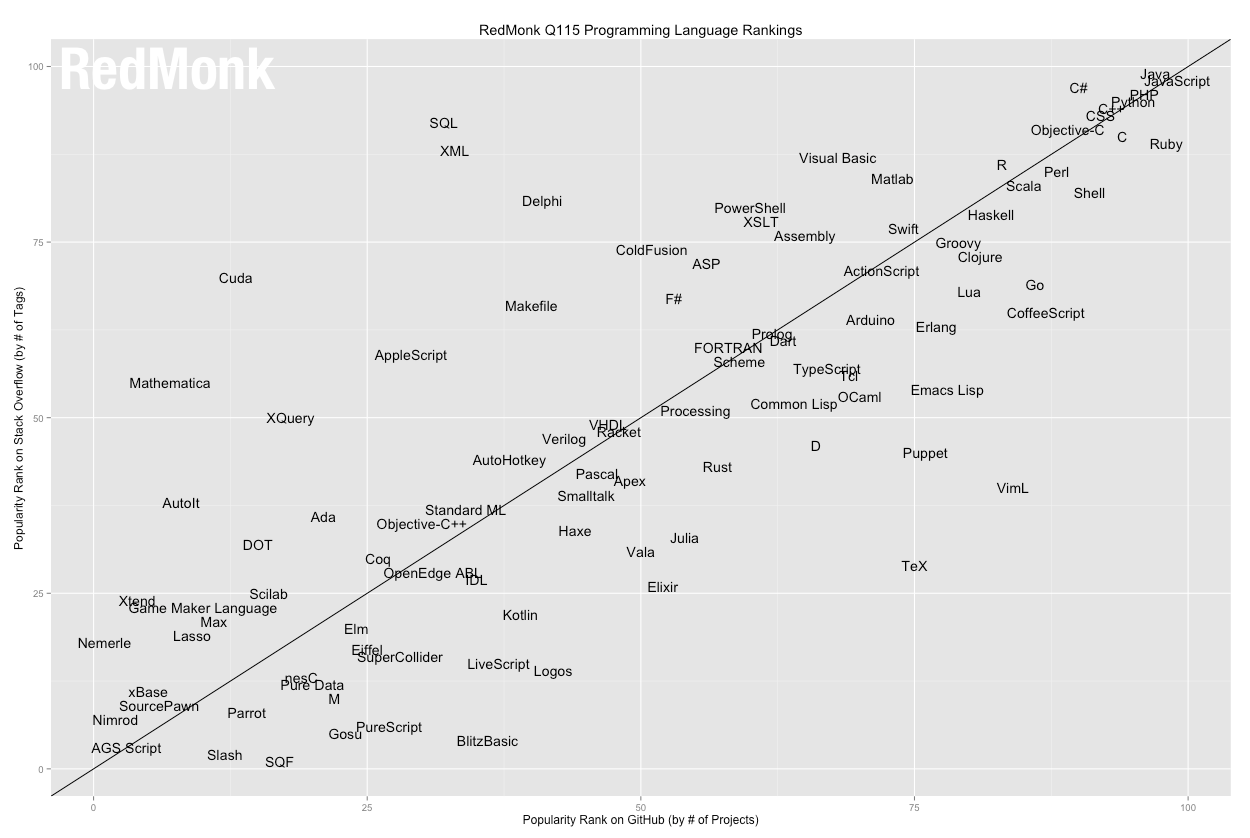
\includegraphics[width=1\textwidth]{img/grafico_redmonk}
	\caption{Ranking das liguagens de programação no Stack Overflow e Github}
\end{figure}


Ainda assim, para compor a interface do dado projeto, também ocorrerá o uso do líder JavaScript de forma intensa, provendo o elo com o as informações gerenciadas pelo PHP.


Entretanto, não seria inteligente desenvolver um sistema completo sem o auxílio de um framework. Dentre os frameworks disponíveis para PHP, hoje o destaque está com o Laravel, que se encontra no topo dentre os mais utilizados no momento. 


A WebHostFace, uma empresa de hospedagem, compilou várias estatísticas para criar um infográfico mostrando os frameworks PHP mais populares de 2015. Utilizando informações sobre os próprios clientes, o Google Trends, estatísticas de repositórios do GitHub e a pesquisa do SitePoint “Best PHP Frameworks 2015”, a WebHostFace elaborou o seguinte infográfico: 

\begin{figure}
	\label{fig:graficoWebhostface}
	\includegraphics[width=1\textwidth]{img/infografico_webhostface}
	\caption{Infográfico da WebhostFace, exibindo a popularidade dos Frameworks PHP em 2015}
\end{figure}

Assim, tem-se a evidência que o Laravel em 2015 teve a maior popularidade em projetos pessoais e tem a maior comunidade entre os concorrentes, o que o torna uma boa escolha para a escrita de um software que será continuado por terceiros.


Para elaborar os recursos de interface e integrar ao back-end PHP do sistema, será adotado o já conhecido AngularJS, ferramenta sólida e conhecida no aspecto em questão. 


Dados coletados via Google Trends, que propõe comparações entre termos pesquisados, revela a popularidade do AngularJs diante de alguns dos principais concorrentes. O gráfico abaixo evidencia o cenário.


%Como mostra a Figura \ref{fig:graficoGoogleTrendsFerramentasFront}. 
\begin{figure}
	\label{fig:graficoGoogleTrendsFerramentasFront}
	\includegraphics[width=1\textwidth]{img/grafico_ferramentas_front}
	\caption{Gráfico do Google Trends exibindo as pesquisas por ferramentas front-end}
\end{figure}


Junto ao Angular JS, será utilizada a agradável tendência de interface do Material Design da Google, que propõe layouts limpos e otimizados já conhecidos pelos usuários de smartphones Android. 


Para a elaboração da plataforma mobile do projeto, será utilizado o Ionic Framework, muito difundido e bastante pesquisado na área, o que fica evidenciado com o gráfico de pesquisbaixo, coletado via Google Trends buscando por frameworks de desenvolvimento híbrido mobile.


\begin{figure}
	\label{fig:graficoGoogleTrendsFerramentasHibridasMobile}
	\includegraphics[width=1\textwidth]{img/grafico_ferramentas_hibridas_mobile}
	\caption{Gráfico do Google Trends exibindo as pesquisas por Frameworks híbridos mobile}
\end{figure}	

Para layout da interface mobile, também será aplicado a tendência do Material Design, a fim de propor uma harmonia entre o módulo web e mobile para os usuários


\section{Resultados Esperados}


Como fruto de um sistema para pós-graduação da UFBA, espera-se que os professores tenham mais recursos para integrar as atividades e também prover melhores condições para acompanhamento da vida acadêmica dos alunos em questão. Também, que os novos colaboradores que entrarem no processo tenham facilidade de compreender o fluxo do setor ao navegar pelo sistema proposto.


\section{Fora de Escopo}


Interação com os alunos devido às complicações para realizar a integração com o sistema empregado na UFBA, gerenciado pela XXXXXX, o que causaria uma inviabilidade no projeto devido à necessidade de entrega do produto ser mais forte que o tempo necessário para executar o processo de obtenção de acesso ao sistema legado para realizar a integração.


\section{Estrutura do Trabalho}


<breve resumo sobre os capítulos do TCC>
\chapter{Referencial Teórico}


Projetar o desenvolvimento de um software requer muito planejamento, pois as falhas iniciais podem custar bastante caro ou até mesmo inviabilizar a continuação de um projeto. Assim, a escolha da arquitetura ideal para a aplicabilidade é essencial na concepção de um produto de software. 
De todo o modo, sempre busca-se fazer mais com menos. Diante de tal filosofia, temos nesta seção, uma breve discussão sobre alguns elementos de projeto e arquitetura de software, a fim de contextualizar este trabalho de conclusão de curso.


% Ser direto no começo, focando no que realmente será discutido A seção \ref{sec:apps_mobile} 
 \section{Software como serviço}\label{sec:saas}


A definição de SaaS encontra-se muito bem elaborada em um dos trabalhos listados na literatura. Segundo La e Chun \citep{La2009Systematic}, o princípio da definição de Software como um Serviço (Sofware as a Service - SaaS) é um serviço complementar para aplicações da computação em nuvem (cloud computing). As duas áreas estão interligadas, no entanto, não se confundem, pois o SaaS deve ser entendido como um mecanismo de suporte às soluções existentes na cloud. Os SaaS existem justamente para maximizar o reuso de serviços repetidos e não centrais em uma aplicação remota.


Como propõe vantagens, software como servico é uma tendência forte, isso graças à evolução da web. Diversos fatores podem ser favoráveis para a adoção de um SaaS, como custo e manutenção dentre outros fatores aplicaveis a determinados contextos. Um trabalho recente realizado por Lechessa et al. \cite{LechesaSS11} apresenta uma pesquisa qualitativa sobre os fatores determinantes para adoção ou não de um SaaS voltado para ERP na África do Sul. Esses autores indicam que os principais fatores determinantes para adoção desse mecanismo de software são sua fluidez quanto à rede e a segurança. Esses fatores estão presentes na aplicação desenvolvida neste trabalho de conclusão de curso.
 

Devido ao fato de ter um serviço constantemente na nuvem, fica o questionamento sobre a segurança da informação manipulada. Sabe-se que a vulnerabilidade na web não é restrita ao SaaS, atingindo diversos âmbitos. O artigo de Rai et al. \cite{journals/corr/RaiSM13} orienta como o avanço da computação em nuvem não é um problema apenas para os serviços web do ponto de vista da segurança, pois muitos trabalhos na literatura mostram a área como mais um ponto de vulnerabilidade para diversos setores, a exemplo de infraestrutura. No mesmo artigo mencionado de Rai et al. \cite{journals/corr/RaiSM13}, também realizaram-se estudos exploratórios junto a empresas usuárias de serviços em computação em nuvem e consideram que a perspectiva de SaaS também pode fortalecer a segurança nas aplicações de cloud computing, pois o software de autenticação compartilhado por várias aplicações em nuvem, oferece uma melhor padronização e consequente facilidade de prevenção a erros de vulnerabilidade específicas de cada módulo da pesquisa. Esse ponto de vista é muito importante para qualquer trabalho de ponta na área de SaaS.


A arquitetura de armazenamento de dados de um Saas pode variar de acordo com a necessidade do contexto. O artigo recente de Huixin \cite{7586486}, exemplifica possíveis modelagens para utilizar. Tal abordagem pode ser com um banco de dados único, fazendo com que diferentes clientes compartilhem o mesmo banco, diferindo os dados através de controle de usuário, ou isolando os diferentes clientes através de bancos de dados exclusivos para cada um. Tal fator também pode ser combinado com a arquitetura da aplicação, caso ofereça aplicação única para todos os clientes ou aplicação compartilhada. Diante das possíveis abprdagens, a modelagem de dados do software pode ser decidida pela regra de negócio. Este trabalho optou por aplicação única e banco de dados compartilhado.


Devido ao diferente conceito de obtenção de software, tanto pela visão do cliente como pela visão do vendedor, é necessário tomar conhecimento dos diversos fatores que podem ser relevantes ao orçar um Saas. O recente trabalho de T. Kaur et al. \citep{6949281} orienta um modelo para compor o custo de um Saas. O custo total seria composto pelos fatores que dão suporte ao funcionamento do software. Tais fatores incluem infra-estrutura, configurabilidade, customização, parâmetros de QoS(Quality of service) como escalabilidade, disponibilidade, usabilidade, pontualidade e desempenho da resposta, portabilidade, custo total de propriedade e retorno do investimento. Esses fatores caracterizam o custo de forma eficaz, possibilitando ao fornecedor, prover um Serviço de acordo com a exigência do consumidor em vários pacotes de serviços.


\section{Reuso de software}\label{sec:reuso} %CRUISE BOOK CAPITULO 2


Para Peter Freeman, o reuso é a utilização de qualquer informação que um desenvolvedor pode necessitar no processo de criação de software (Ezran et al., 2002). Basili e Rombach definem reutilização de software como o uso de tudo o que está associado a um projeto de conhecimento (Basili e Rombach, 1991).
Assim, o objetivo da reutilização de software é reciclar o design, código e outros componentes de um produto de software e assim reduzir o custo, o tempo e melhorar a qualidade do produto.
Segundo Keswani et al. \cite{6783445}, o componente reutilizável de software pode ser qualquer parte de seu desenvolvimento, como um fragmento de código, design, casos de teste, ou até mesmo a especificação de requisitos de uma funcionalidade do software. 

O reuso de software pode ter impacto positivo em diversos aspectos do software, vejamos alguns, conforme apresentados no C.R.U.I.S.E Book:

\begin{itemize}

\item Qualidade: As correções de erro tornam-se úteis em todos os locais em que ocorreu, padronizando e facilitando a manutenção.

\item Produtividade: O ganho de produtividade é alcançado devido ao menor número de artefatos desenvolvido. Isso resulta em menos esforços de teste e também economiza análise e design, gerando economia em diversos escopos do projeto.

\item Confiabilidade: A utilização de componentes bem testados aumenta a
confiança no software. Além disso, a utilização de um mesmo componente em vários sistemas, aumenta a possibilidade de detecção de erros e reforça a confiança no componente.

\item Redução do Esforço: A reutilização de software proporciona uma redução do tempo de desenvolvimento, o que reduz o tempo necessário para o produto ser disponibilizado no mercado para trazer rentabilidade.

\item Trabalho redundante e tempo de desenvolvimento: Desenvolver um sistema do
zero significa desenvolvimento redundante de muitos componentes, como requisito
especificações, casos de uso, arquitetura, etc. Isso pode ser evitado quando estes estão disponíveis como componentes reutilizáveis e podem ser compartilhados, resultando em menos desenvolvimento, tempo e custo associado.

\item Documentação: Embora a documentação seja muito importante para a
manutenção de um sistema, muitas vezes é negligenciada. A reutilização de componentes software reduz a quantidade de documentação a ser escrita, entretanto depende da qualidade do que está escrito. Assim, apenas a estrutura do sistema e os novos artefatos desenvolvidos necessitam ser documentados.

\item Custo de manutenção: Menos defeitos e manutenções são esperados quando tem-se comprovada a qualidade dos componentes utilizados.

\item Tamanho da equipe: É comum entrar casos em que a equipe de desenvolvimento sofre sobrecarga. Entretanto, dobrar o tamanho da equipe de desenvolvimento não necessariamente duplica produtividade. Se muitos componentes podem ser reutilizados, é possível desenvolver com equipes menores, levando a melhores comunicações e aumento da produtividade.

\end{itemize}

Apesar dos benefícios da reutilização de software, a mesma não é amplamente praticado como imagina-se. Existem fatores que influenciam direta ou indiretamente na sua adoção. Esses fatores podem ser de aspecto gerencial, organizacional, econômico, conceitual ou técnico. Veremos a seguir alguns aspectos que podem gerar conflito com a cultura de reuso de software, segundo o C.R.U.I.S.E Book:
%(Sametinger, 1997). REVER

\begin{itemize}
	
\item Falta de apoio da gestão: Como a reutilização de software gera custos iniciais,
a medida pode não ser amplamente alcançada em uma organização sem o apoio de alto nível gestão. Os gestores têm de ser informados sobre os custos iniciais e serem convencidos sobre economias futuras.

\item Gerenciamento do Projeto: Gerenciar projetos tradicionais é uma tarefa árdua, principalmente, os que praticam a reutilização de software. Utilizando a técnica em larga escala, tem-se impacto sobre todo o ciclo de vida do software.

\item Estruturas organizacionais inadequadas: As estruturas organizacionais devem
considerar diferentes necessidades que surgem quando a reutilização em larga escala está sendo adotada. Por exemplo, uma equipe particionada pode ser alocada somente para desenvolver, manter e certificar componentes reutilizáveis de software.

\item Incentivos de gestão: É comum a falta de incentivo para deixar os desenvolvedores gastarem tempo elaborando reutilizáveis componentes do sistema. A produtividade é muitas vezes medida apenas no tempo necessário para concluir um projeto. Assim, fazer qualquer trabalho além disso, embora benéfico para a empresa como um todo, diminui o seu sucesso. Mesmo quando os componentes reutilizáveis são utilizados, os benefícios obtidos são uma pequena fração do que poderia ser alcançado caso houvesse reutilização explícita, planejada e organizada.

\item Dificuldade de encontrar software reutilizável: Para reutilizar os componentes, devem existir formas eficientes de busca. Além disso, é importante ter um repositório bem organizado contendo componentes com um eficiente meio de acesso.

\item Não reutilização do software encontrado. O acesso fácil ao software existente
não necessariamente aumentar a reutilização. Os componentes reutilizáveis devem ser cuidadosamente especificados, projetados, implementados e documentados, pois em alguns casos, modificar e adaptar o código  pode ser mais custoso que a programação da funcionalidade necessária a partir do zero.

\item Modificação: É muito difícil encontrar um componente que funcione
exatamente da mesma maneira que queremos. Desta forma, são necessárias modificações e devem existir formas de determinar os seus efeitos sobre o componente.


\end{itemize}


%Outra diretriz importante para a reutilização de software é reduzir o risco na criação de novos softwares. O risco tende a ser bastante reduzido se os componentes que estão sendo reutilizados têm as documentação, interfaces necessárias e devidamente testadas, fatores que contibruem para uma fácil integração.
%De acordo com Keswani et al. \citep{6783445}, para o reuso de software dar retornos apropriados, o processo deve ser sistemático e planejado. Qualquer organização que implemente a reutilização de software deve identificar os melhores métodos e estratégias de reutilização para obter a máxima produtividade. A reutilização de software ajuda a evitar software de engenharia a partir do zero, pois usa módulos de software existentes. A reutilização de software, embora seja uma tarefa difícil, especialmente para softwares antigos sem padrões de projeto, pode melhorar significativamente a produtividade e a qualidade de um produto de software. Embora a reutilização de software não seja um novo campo, ela pode dar grandes retornos em curto período de tempo.


\section{Modularização}\label{sec:modularizacao} %artigo de claudio pagina 222 introdução


%A modularidade vem desempenhando um papel predominante estágios emergentes das disciplinas de arquitetura de software [13]. Engenheiros de software consideram modularidade como princípio base na comparação entre arquiteturas alternativas  e arquitetura degeneração [9]. De fato, os engenheiros de software são incentivados a arquitecturas, baseando-se numa multiplicidade de mecanismos de modularidade disponíveis em: 
%(i) Linguagens de descrição de arquitetura (ADLs), como ACME [8], 
%(ii) catálogos de arquitetônicos [2, 13], e 
%(iii) conhecem bem princípios de alto nível, como interfaces de componentes estreitos, acoplamento arquitectónico reduzido e semelhantes.


Conforme é frisado no trabalho de Wickramaarachchi e Lai \citep{7062705}, o conceito de modularização na indústria de software tem uma longa história e tem sido utilizado para melhorar o processo de desenvolvimento de software em diferentes estágios. Os principais conceitos por trás da modularização do software foram introduzidos por pesquisadores pioneiros há quarenta anos, com uma notável contribuição feita por Melvin Conway e David Parnas, que tem representação notável na engenharia de software.


Modularizar um software é um bom padrão a ser adotado. Segundo Wickramaarachchi e Lai \citep{7062705}, a modularização é importante na identificação de dependências e reduz as dificuldades diante de uma possível necessidade de grandes alterações. De uma perspectiva da engenharia de software, uma modularização geralmente tem várias vantagens, tais como: tornar a complexidade do software mais gerenciável, facilitar o trabalho paralelo e tornar o software mais maleável para acomodar o futuro incerto que um software pode ter. O objetivo final da modularização do software é aumentar a produtividade ea qualidade do software. Tal conceito encontra-se bastante difundido e estái incorporado em linguagens de programação e ferramentas de software. O trabalho proposto favorece ao uso da modularização de um software e até mesmo pode ser considerado um módulo a ser acoplado a qualquer software, mediante a compatibilidade.


\section{Aplicações web}\label{sec:apps_web}


A popularidade da aplicação web aumentou exponencialmente na última década e todos os dias cresce o número de pessoas usuárias de aplicações web. E seguindo o padrão de desenvolvimento de software, Kumar et al. \citep{7813710} sugerem que para o desenvolvimento web, deve-se manter a prática efiacaz de produzir diagramas UML. A abordagem baseada na web oferece uma maneira fácil e eficaz para gerenciar e controlar o processo de desenvolvimento por meio de diagramas UML. Tal abordagem pode ser usada quando há uma exigência de lidar com mudanças muito rápidas e grandes em requisitos de forma muito eficaz em muito menos tempo, gerando assim um menor impacto. 


Para atender à fomentada demanda de aplicativos web, é necessário adotar métodos de desenvolvimentos que sejam ágeis, eficientes e de fácil manutenção. Yu Ping et al. \cite{1372143} propõem o uso do modelo MVC (Model, View e Controller) no atual desenvolvimento para softwares web. O modelo apresentado tornou-se um padrão popular e divide o software em camadas com propósito definido, tornando-o de mais fácil manutenção.


O Ajax (Asynchronous Javascript and XML) revolucionou a web. Conforme demonstrado no artigo de Yuping \citep{6845605}, ao usar a tecnologia Ajax, podemos enriquecer a experiência do usuário em aplicações baseadas em navegador de internet, e fornecer uma variedade de aplicações interativas para atender às necessidade de humanização das aplicações.
Os aplicativos Ajax em execução no navegador se comunicam com um servidor Web de forma assíncrona e atualizam apenas uma parte da página.



% %% RiSE Latex Template - version 0.5
%%
%% RiSE's latex template for thesis and dissertations
%% http://risetemplate.sourceforge.net
%%
%% (c) 2012 Yguaratã Cerqueira Cavalcanti (yguarata@gmail.com)
%%          Vinicius Cardoso Garcia (vinicius.garcia@gmail.com)
%%
%% This document was initially based on UFPEThesis template, from Paulo Gustavo
%% S. Fonseca.
%%
%% ACKNOWLEDGEMENTS
%%
%% We would like to thanks the RiSE's researchers community, the 
%% students from Federal University of Pernambuco, and other users that have
%% been contributing to this projects with comments and patches.
%%
%% GENERAL INSTRUCTIONS
%%
%% We strongly recommend you to compile your documents using pdflatex command.
%% It is also recommend use the texlipse plugin for Eclipse to edit your documents.
%%
%% Options for \documentclass command:
%%         * Idiom
%%           pt   - Portguese (default)
%%           en   - English
%%
%%         * Text type
%%           bsc  - B.Sc. Thesis
%%           msc  - M.Sc. Thesis (default)
%%           qual - PHD qualification (not tested yet)
%%           prop - PHD proposal (not tested yet)
%%           phd  - PHD thesis
%%
%%         * Media
%%           scr  - to eletronic version (PDF) / see the users guide
%%
%%         * Pagination
%%           oneside - unique face press
%%           twoside - two faces press
%%
%%		   * Line spacing
%%           singlespacing  - the same as using \linespread{1}
%%           onehalfspacing - the same as using \linespread{1.3}
%%           doublespacing  - the same as using \linespread{1.6}
%%
%% Reference commands. Use the following commands to make references in your
%% text:
%%          \figref  -- for Figure reference
%%          \tabref  -- for Table reference
%%          \eqnref  -- for equation reference
%%          \chapref -- for chapter reference
%%          \secref  -- for section reference
%%          \appref  -- for appendix reference
%%          \axiref  -- for axiom reference
%%          \conjref -- for conjecture reference
%%          \defref  -- for definition reference
%%          \lemref  -- for lemma reference
%%          \theoref -- for theorem reference
%%          \corref  -- for corollary reference
%%          \propref -- for proprosition reference
%%          \pgref   -- for page reference
%%
%%          Example: See \chapref{chap:introduction}. It will produce 
%%                   'See Chapter 1', in case of English language.

\documentclass[pt,twoside,onehalfspacing,bsc]{risethesis}

\usepackage[utf8]{inputenc}
\usepackage[brazilian]{babel}
\usepackage[T1]{fontenc}

%% Change the following pdf author attribute name to your name.
\usepackage[linkcolor=blue,citecolor=blue,urlcolor=blue,colorlinks,pdfpagelabels,pdftitle={Bruno Cabral's Bachelor Thesis},pdfauthor={Bruno Cabral}]{hyperref}

\address{SALVADOR}

\universitypt{Universidade Federal da Bahia}
\universityen{Federal University of Bahia}

\departmentpt{Depertamento de Ciência da Computação}
\departmenten{Computer Science Department}

\programpt{Programa Multiinstitucional de Pós-graduação em Ciência da Computação}
\programen{Graduate in Computer Science}

\majorfieldpt{Ciência da Computação}
\majorfielden{Computer Science}

\title{Sistema de apoio à Pós graduação - UFBA}
\date{Outubro/2016}

\author{Victor de Azevedo Nunes}
\adviser{Ivan do Carmo Machado}

\begin{document}

\frontmatter
\frontpage
\presentationpage

\begin{dedicatory}
Eu dedico esta dissertação...
%I dedicate this dissertation to my family, girlfriend, friends and
%professors who gave me all necessary support to get here.
\end{dedicatory}

\acknowledgements
Meus agradecimentos...

\begin{epigraph}[]{Edward V Berard}
Walking on water and developing software from a specification are easy if both are frozen
\end{epigraph}

\resumo
% Escreva seu resumo no arquivo resumo.tex
\input{resumo}

\abstract
% Write your abstract in a file called abstract.tex
\input{abstract}

% Summary (tables of contents)
\tableofcontents

% List of figures
\listoffigures

% List of tables
\listoftables

% List of acronyms
% Acronyms manual: http://linorg.usp.br/CTAN/macros/latex/contrib/acronym/acronym.pdf
\listofacronyms
\input{acronyms}

% List of listings
%\lstlistoflistings

\mainmatter

\include{chapters/intro}
\include{chapters/referencial_teorico}

% \include{chapters/introduction/main}
% \include{chapters/background/main}
% \include{chapters/proposed_solution/main}
% \include{chapters/experiment/main}
% \include{chapters/conclusion/main}

\bibliographystyle{natbib}
\addcontentsline{toc}{chapter}{\bibliographytocname}
\bibliography{references}

% Appendix
\clearpage
\addappheadtotoc
\appendix
\appendixpage
% \include{appendix/experiment-instruments}

\end{document}
% %% RiSE Latex Template - version 0.5
%%
%% RiSE's latex template for thesis and dissertations
%% http://risetemplate.sourceforge.net
%%
%% (c) 2012 Yguaratã Cerqueira Cavalcanti (yguarata@gmail.com)
%%          Vinicius Cardoso Garcia (vinicius.garcia@gmail.com)
%%
%% This document was initially based on UFPEThesis template, from Paulo Gustavo
%% S. Fonseca.
%%
%% ACKNOWLEDGEMENTS
%%
%% We would like to thanks the RiSE's researchers community, the 
%% students from Federal University of Pernambuco, and other users that have
%% been contributing to this projects with comments and patches.
%%
%% GENERAL INSTRUCTIONS
%%
%% We strongly recommend you to compile your documents using pdflatex command.
%% It is also recommend use the texlipse plugin for Eclipse to edit your documents.
%%
%% Options for \documentclass command:
%%         * Idiom
%%           pt   - Portguese (default)
%%           en   - English
%%
%%         * Text type
%%           bsc  - B.Sc. Thesis
%%           msc  - M.Sc. Thesis (default)
%%           qual - PHD qualification (not tested yet)
%%           prop - PHD proposal (not tested yet)
%%           phd  - PHD thesis
%%
%%         * Media
%%           scr  - to eletronic version (PDF) / see the users guide
%%
%%         * Pagination
%%           oneside - unique face press
%%           twoside - two faces press
%%
%%		   * Line spacing
%%           singlespacing  - the same as using \linespread{1}
%%           onehalfspacing - the same as using \linespread{1.3}
%%           doublespacing  - the same as using \linespread{1.6}
%%
%% Reference commands. Use the following commands to make references in your
%% text:
%%          \figref  -- for Figure reference
%%          \tabref  -- for Table reference
%%          \eqnref  -- for equation reference
%%          \chapref -- for chapter reference
%%          \secref  -- for section reference
%%          \appref  -- for appendix reference
%%          \axiref  -- for axiom reference
%%          \conjref -- for conjecture reference
%%          \defref  -- for definition reference
%%          \lemref  -- for lemma reference
%%          \theoref -- for theorem reference
%%          \corref  -- for corollary reference
%%          \propref -- for proprosition reference
%%          \pgref   -- for page reference
%%
%%          Example: See \chapref{chap:introduction}. It will produce 
%%                   'See Chapter 1', in case of English language.

\documentclass[pt,twoside,onehalfspacing,bsc]{risethesis}

\usepackage[utf8]{inputenc}
\usepackage[brazilian]{babel}
\usepackage[T1]{fontenc}

%% Change the following pdf author attribute name to your name.
\usepackage[linkcolor=blue,citecolor=blue,urlcolor=blue,colorlinks,pdfpagelabels,pdftitle={Bruno Cabral's Bachelor Thesis},pdfauthor={Bruno Cabral}]{hyperref}

\address{SALVADOR}

\universitypt{Universidade Federal da Bahia}
\universityen{Federal University of Bahia}

\departmentpt{Depertamento de Ciência da Computação}
\departmenten{Computer Science Department}

\programpt{Programa Multiinstitucional de Pós-graduação em Ciência da Computação}
\programen{Graduate in Computer Science}

\majorfieldpt{Ciência da Computação}
\majorfielden{Computer Science}

\title{Sistema de apoio à Pós graduação - UFBA}
\date{Outubro/2016}

\author{Victor de Azevedo Nunes}
\adviser{Ivan do Carmo Machado}

\begin{document}

\frontmatter
\frontpage
\presentationpage

\begin{dedicatory}
Eu dedico esta dissertação...
%I dedicate this dissertation to my family, girlfriend, friends and
%professors who gave me all necessary support to get here.
\end{dedicatory}

\acknowledgements
Meus agradecimentos...

\begin{epigraph}[]{Edward V Berard}
Walking on water and developing software from a specification are easy if both are frozen
\end{epigraph}

\resumo
% Escreva seu resumo no arquivo resumo.tex
\input{resumo}

\abstract
% Write your abstract in a file called abstract.tex
\input{abstract}

% Summary (tables of contents)
\tableofcontents

% List of figures
\listoffigures

% List of tables
\listoftables

% List of acronyms
% Acronyms manual: http://linorg.usp.br/CTAN/macros/latex/contrib/acronym/acronym.pdf
\listofacronyms
\input{acronyms}

% List of listings
%\lstlistoflistings

\mainmatter

\include{chapters/intro}
\include{chapters/referencial_teorico}

% \include{chapters/introduction/main}
% \include{chapters/background/main}
% \include{chapters/proposed_solution/main}
% \include{chapters/experiment/main}
% \include{chapters/conclusion/main}

\bibliographystyle{natbib}
\addcontentsline{toc}{chapter}{\bibliographytocname}
\bibliography{references}

% Appendix
\clearpage
\addappheadtotoc
\appendix
\appendixpage
% \include{appendix/experiment-instruments}

\end{document}
% %% RiSE Latex Template - version 0.5
%%
%% RiSE's latex template for thesis and dissertations
%% http://risetemplate.sourceforge.net
%%
%% (c) 2012 Yguaratã Cerqueira Cavalcanti (yguarata@gmail.com)
%%          Vinicius Cardoso Garcia (vinicius.garcia@gmail.com)
%%
%% This document was initially based on UFPEThesis template, from Paulo Gustavo
%% S. Fonseca.
%%
%% ACKNOWLEDGEMENTS
%%
%% We would like to thanks the RiSE's researchers community, the 
%% students from Federal University of Pernambuco, and other users that have
%% been contributing to this projects with comments and patches.
%%
%% GENERAL INSTRUCTIONS
%%
%% We strongly recommend you to compile your documents using pdflatex command.
%% It is also recommend use the texlipse plugin for Eclipse to edit your documents.
%%
%% Options for \documentclass command:
%%         * Idiom
%%           pt   - Portguese (default)
%%           en   - English
%%
%%         * Text type
%%           bsc  - B.Sc. Thesis
%%           msc  - M.Sc. Thesis (default)
%%           qual - PHD qualification (not tested yet)
%%           prop - PHD proposal (not tested yet)
%%           phd  - PHD thesis
%%
%%         * Media
%%           scr  - to eletronic version (PDF) / see the users guide
%%
%%         * Pagination
%%           oneside - unique face press
%%           twoside - two faces press
%%
%%		   * Line spacing
%%           singlespacing  - the same as using \linespread{1}
%%           onehalfspacing - the same as using \linespread{1.3}
%%           doublespacing  - the same as using \linespread{1.6}
%%
%% Reference commands. Use the following commands to make references in your
%% text:
%%          \figref  -- for Figure reference
%%          \tabref  -- for Table reference
%%          \eqnref  -- for equation reference
%%          \chapref -- for chapter reference
%%          \secref  -- for section reference
%%          \appref  -- for appendix reference
%%          \axiref  -- for axiom reference
%%          \conjref -- for conjecture reference
%%          \defref  -- for definition reference
%%          \lemref  -- for lemma reference
%%          \theoref -- for theorem reference
%%          \corref  -- for corollary reference
%%          \propref -- for proprosition reference
%%          \pgref   -- for page reference
%%
%%          Example: See \chapref{chap:introduction}. It will produce 
%%                   'See Chapter 1', in case of English language.

\documentclass[pt,twoside,onehalfspacing,bsc]{risethesis}

\usepackage[utf8]{inputenc}
\usepackage[brazilian]{babel}
\usepackage[T1]{fontenc}

%% Change the following pdf author attribute name to your name.
\usepackage[linkcolor=blue,citecolor=blue,urlcolor=blue,colorlinks,pdfpagelabels,pdftitle={Bruno Cabral's Bachelor Thesis},pdfauthor={Bruno Cabral}]{hyperref}

\address{SALVADOR}

\universitypt{Universidade Federal da Bahia}
\universityen{Federal University of Bahia}

\departmentpt{Depertamento de Ciência da Computação}
\departmenten{Computer Science Department}

\programpt{Programa Multiinstitucional de Pós-graduação em Ciência da Computação}
\programen{Graduate in Computer Science}

\majorfieldpt{Ciência da Computação}
\majorfielden{Computer Science}

\title{Sistema de apoio à Pós graduação - UFBA}
\date{Outubro/2016}

\author{Victor de Azevedo Nunes}
\adviser{Ivan do Carmo Machado}

\begin{document}

\frontmatter
\frontpage
\presentationpage

\begin{dedicatory}
Eu dedico esta dissertação...
%I dedicate this dissertation to my family, girlfriend, friends and
%professors who gave me all necessary support to get here.
\end{dedicatory}

\acknowledgements
Meus agradecimentos...

\begin{epigraph}[]{Edward V Berard}
Walking on water and developing software from a specification are easy if both are frozen
\end{epigraph}

\resumo
% Escreva seu resumo no arquivo resumo.tex
\input{resumo}

\abstract
% Write your abstract in a file called abstract.tex
\input{abstract}

% Summary (tables of contents)
\tableofcontents

% List of figures
\listoffigures

% List of tables
\listoftables

% List of acronyms
% Acronyms manual: http://linorg.usp.br/CTAN/macros/latex/contrib/acronym/acronym.pdf
\listofacronyms
\input{acronyms}

% List of listings
%\lstlistoflistings

\mainmatter

\include{chapters/intro}
\include{chapters/referencial_teorico}

% \include{chapters/introduction/main}
% \include{chapters/background/main}
% \include{chapters/proposed_solution/main}
% \include{chapters/experiment/main}
% \include{chapters/conclusion/main}

\bibliographystyle{natbib}
\addcontentsline{toc}{chapter}{\bibliographytocname}
\bibliography{references}

% Appendix
\clearpage
\addappheadtotoc
\appendix
\appendixpage
% \include{appendix/experiment-instruments}

\end{document}
% %% RiSE Latex Template - version 0.5
%%
%% RiSE's latex template for thesis and dissertations
%% http://risetemplate.sourceforge.net
%%
%% (c) 2012 Yguaratã Cerqueira Cavalcanti (yguarata@gmail.com)
%%          Vinicius Cardoso Garcia (vinicius.garcia@gmail.com)
%%
%% This document was initially based on UFPEThesis template, from Paulo Gustavo
%% S. Fonseca.
%%
%% ACKNOWLEDGEMENTS
%%
%% We would like to thanks the RiSE's researchers community, the 
%% students from Federal University of Pernambuco, and other users that have
%% been contributing to this projects with comments and patches.
%%
%% GENERAL INSTRUCTIONS
%%
%% We strongly recommend you to compile your documents using pdflatex command.
%% It is also recommend use the texlipse plugin for Eclipse to edit your documents.
%%
%% Options for \documentclass command:
%%         * Idiom
%%           pt   - Portguese (default)
%%           en   - English
%%
%%         * Text type
%%           bsc  - B.Sc. Thesis
%%           msc  - M.Sc. Thesis (default)
%%           qual - PHD qualification (not tested yet)
%%           prop - PHD proposal (not tested yet)
%%           phd  - PHD thesis
%%
%%         * Media
%%           scr  - to eletronic version (PDF) / see the users guide
%%
%%         * Pagination
%%           oneside - unique face press
%%           twoside - two faces press
%%
%%		   * Line spacing
%%           singlespacing  - the same as using \linespread{1}
%%           onehalfspacing - the same as using \linespread{1.3}
%%           doublespacing  - the same as using \linespread{1.6}
%%
%% Reference commands. Use the following commands to make references in your
%% text:
%%          \figref  -- for Figure reference
%%          \tabref  -- for Table reference
%%          \eqnref  -- for equation reference
%%          \chapref -- for chapter reference
%%          \secref  -- for section reference
%%          \appref  -- for appendix reference
%%          \axiref  -- for axiom reference
%%          \conjref -- for conjecture reference
%%          \defref  -- for definition reference
%%          \lemref  -- for lemma reference
%%          \theoref -- for theorem reference
%%          \corref  -- for corollary reference
%%          \propref -- for proprosition reference
%%          \pgref   -- for page reference
%%
%%          Example: See \chapref{chap:introduction}. It will produce 
%%                   'See Chapter 1', in case of English language.

\documentclass[pt,twoside,onehalfspacing,bsc]{risethesis}

\usepackage[utf8]{inputenc}
\usepackage[brazilian]{babel}
\usepackage[T1]{fontenc}

%% Change the following pdf author attribute name to your name.
\usepackage[linkcolor=blue,citecolor=blue,urlcolor=blue,colorlinks,pdfpagelabels,pdftitle={Bruno Cabral's Bachelor Thesis},pdfauthor={Bruno Cabral}]{hyperref}

\address{SALVADOR}

\universitypt{Universidade Federal da Bahia}
\universityen{Federal University of Bahia}

\departmentpt{Depertamento de Ciência da Computação}
\departmenten{Computer Science Department}

\programpt{Programa Multiinstitucional de Pós-graduação em Ciência da Computação}
\programen{Graduate in Computer Science}

\majorfieldpt{Ciência da Computação}
\majorfielden{Computer Science}

\title{Sistema de apoio à Pós graduação - UFBA}
\date{Outubro/2016}

\author{Victor de Azevedo Nunes}
\adviser{Ivan do Carmo Machado}

\begin{document}

\frontmatter
\frontpage
\presentationpage

\begin{dedicatory}
Eu dedico esta dissertação...
%I dedicate this dissertation to my family, girlfriend, friends and
%professors who gave me all necessary support to get here.
\end{dedicatory}

\acknowledgements
Meus agradecimentos...

\begin{epigraph}[]{Edward V Berard}
Walking on water and developing software from a specification are easy if both are frozen
\end{epigraph}

\resumo
% Escreva seu resumo no arquivo resumo.tex
\input{resumo}

\abstract
% Write your abstract in a file called abstract.tex
\input{abstract}

% Summary (tables of contents)
\tableofcontents

% List of figures
\listoffigures

% List of tables
\listoftables

% List of acronyms
% Acronyms manual: http://linorg.usp.br/CTAN/macros/latex/contrib/acronym/acronym.pdf
\listofacronyms
\input{acronyms}

% List of listings
%\lstlistoflistings

\mainmatter

\include{chapters/intro}
\include{chapters/referencial_teorico}

% \include{chapters/introduction/main}
% \include{chapters/background/main}
% \include{chapters/proposed_solution/main}
% \include{chapters/experiment/main}
% \include{chapters/conclusion/main}

\bibliographystyle{natbib}
\addcontentsline{toc}{chapter}{\bibliographytocname}
\bibliography{references}

% Appendix
\clearpage
\addappheadtotoc
\appendix
\appendixpage
% \include{appendix/experiment-instruments}

\end{document}
% %% RiSE Latex Template - version 0.5
%%
%% RiSE's latex template for thesis and dissertations
%% http://risetemplate.sourceforge.net
%%
%% (c) 2012 Yguaratã Cerqueira Cavalcanti (yguarata@gmail.com)
%%          Vinicius Cardoso Garcia (vinicius.garcia@gmail.com)
%%
%% This document was initially based on UFPEThesis template, from Paulo Gustavo
%% S. Fonseca.
%%
%% ACKNOWLEDGEMENTS
%%
%% We would like to thanks the RiSE's researchers community, the 
%% students from Federal University of Pernambuco, and other users that have
%% been contributing to this projects with comments and patches.
%%
%% GENERAL INSTRUCTIONS
%%
%% We strongly recommend you to compile your documents using pdflatex command.
%% It is also recommend use the texlipse plugin for Eclipse to edit your documents.
%%
%% Options for \documentclass command:
%%         * Idiom
%%           pt   - Portguese (default)
%%           en   - English
%%
%%         * Text type
%%           bsc  - B.Sc. Thesis
%%           msc  - M.Sc. Thesis (default)
%%           qual - PHD qualification (not tested yet)
%%           prop - PHD proposal (not tested yet)
%%           phd  - PHD thesis
%%
%%         * Media
%%           scr  - to eletronic version (PDF) / see the users guide
%%
%%         * Pagination
%%           oneside - unique face press
%%           twoside - two faces press
%%
%%		   * Line spacing
%%           singlespacing  - the same as using \linespread{1}
%%           onehalfspacing - the same as using \linespread{1.3}
%%           doublespacing  - the same as using \linespread{1.6}
%%
%% Reference commands. Use the following commands to make references in your
%% text:
%%          \figref  -- for Figure reference
%%          \tabref  -- for Table reference
%%          \eqnref  -- for equation reference
%%          \chapref -- for chapter reference
%%          \secref  -- for section reference
%%          \appref  -- for appendix reference
%%          \axiref  -- for axiom reference
%%          \conjref -- for conjecture reference
%%          \defref  -- for definition reference
%%          \lemref  -- for lemma reference
%%          \theoref -- for theorem reference
%%          \corref  -- for corollary reference
%%          \propref -- for proprosition reference
%%          \pgref   -- for page reference
%%
%%          Example: See \chapref{chap:introduction}. It will produce 
%%                   'See Chapter 1', in case of English language.

\documentclass[pt,twoside,onehalfspacing,bsc]{risethesis}

\usepackage[utf8]{inputenc}
\usepackage[brazilian]{babel}
\usepackage[T1]{fontenc}

%% Change the following pdf author attribute name to your name.
\usepackage[linkcolor=blue,citecolor=blue,urlcolor=blue,colorlinks,pdfpagelabels,pdftitle={Bruno Cabral's Bachelor Thesis},pdfauthor={Bruno Cabral}]{hyperref}

\address{SALVADOR}

\universitypt{Universidade Federal da Bahia}
\universityen{Federal University of Bahia}

\departmentpt{Depertamento de Ciência da Computação}
\departmenten{Computer Science Department}

\programpt{Programa Multiinstitucional de Pós-graduação em Ciência da Computação}
\programen{Graduate in Computer Science}

\majorfieldpt{Ciência da Computação}
\majorfielden{Computer Science}

\title{Sistema de apoio à Pós graduação - UFBA}
\date{Outubro/2016}

\author{Victor de Azevedo Nunes}
\adviser{Ivan do Carmo Machado}

\begin{document}

\frontmatter
\frontpage
\presentationpage

\begin{dedicatory}
Eu dedico esta dissertação...
%I dedicate this dissertation to my family, girlfriend, friends and
%professors who gave me all necessary support to get here.
\end{dedicatory}

\acknowledgements
Meus agradecimentos...

\begin{epigraph}[]{Edward V Berard}
Walking on water and developing software from a specification are easy if both are frozen
\end{epigraph}

\resumo
% Escreva seu resumo no arquivo resumo.tex
\input{resumo}

\abstract
% Write your abstract in a file called abstract.tex
\input{abstract}

% Summary (tables of contents)
\tableofcontents

% List of figures
\listoffigures

% List of tables
\listoftables

% List of acronyms
% Acronyms manual: http://linorg.usp.br/CTAN/macros/latex/contrib/acronym/acronym.pdf
\listofacronyms
\input{acronyms}

% List of listings
%\lstlistoflistings

\mainmatter

\include{chapters/intro}
\include{chapters/referencial_teorico}

% \include{chapters/introduction/main}
% \include{chapters/background/main}
% \include{chapters/proposed_solution/main}
% \include{chapters/experiment/main}
% \include{chapters/conclusion/main}

\bibliographystyle{natbib}
\addcontentsline{toc}{chapter}{\bibliographytocname}
\bibliography{references}

% Appendix
\clearpage
\addappheadtotoc
\appendix
\appendixpage
% \include{appendix/experiment-instruments}

\end{document}

\bibliographystyle{natbib}
\addcontentsline{toc}{chapter}{\bibliographytocname}
\bibliography{references}

% Appendix
\clearpage
\addappheadtotoc
\appendix
\appendixpage
% \include{appendix/experiment-instruments}

\end{document}
% %% RiSE Latex Template - version 0.5
%%
%% RiSE's latex template for thesis and dissertations
%% http://risetemplate.sourceforge.net
%%
%% (c) 2012 Yguaratã Cerqueira Cavalcanti (yguarata@gmail.com)
%%          Vinicius Cardoso Garcia (vinicius.garcia@gmail.com)
%%
%% This document was initially based on UFPEThesis template, from Paulo Gustavo
%% S. Fonseca.
%%
%% ACKNOWLEDGEMENTS
%%
%% We would like to thanks the RiSE's researchers community, the 
%% students from Federal University of Pernambuco, and other users that have
%% been contributing to this projects with comments and patches.
%%
%% GENERAL INSTRUCTIONS
%%
%% We strongly recommend you to compile your documents using pdflatex command.
%% It is also recommend use the texlipse plugin for Eclipse to edit your documents.
%%
%% Options for \documentclass command:
%%         * Idiom
%%           pt   - Portguese (default)
%%           en   - English
%%
%%         * Text type
%%           bsc  - B.Sc. Thesis
%%           msc  - M.Sc. Thesis (default)
%%           qual - PHD qualification (not tested yet)
%%           prop - PHD proposal (not tested yet)
%%           phd  - PHD thesis
%%
%%         * Media
%%           scr  - to eletronic version (PDF) / see the users guide
%%
%%         * Pagination
%%           oneside - unique face press
%%           twoside - two faces press
%%
%%		   * Line spacing
%%           singlespacing  - the same as using \linespread{1}
%%           onehalfspacing - the same as using \linespread{1.3}
%%           doublespacing  - the same as using \linespread{1.6}
%%
%% Reference commands. Use the following commands to make references in your
%% text:
%%          \figref  -- for Figure reference
%%          \tabref  -- for Table reference
%%          \eqnref  -- for equation reference
%%          \chapref -- for chapter reference
%%          \secref  -- for section reference
%%          \appref  -- for appendix reference
%%          \axiref  -- for axiom reference
%%          \conjref -- for conjecture reference
%%          \defref  -- for definition reference
%%          \lemref  -- for lemma reference
%%          \theoref -- for theorem reference
%%          \corref  -- for corollary reference
%%          \propref -- for proprosition reference
%%          \pgref   -- for page reference
%%
%%          Example: See \chapref{chap:introduction}. It will produce 
%%                   'See Chapter 1', in case of English language.

\documentclass[pt,twoside,onehalfspacing,bsc]{risethesis}

\usepackage[utf8]{inputenc}
\usepackage[brazilian]{babel}
\usepackage[T1]{fontenc}

%% Change the following pdf author attribute name to your name.
\usepackage[linkcolor=blue,citecolor=blue,urlcolor=blue,colorlinks,pdfpagelabels,pdftitle={Bruno Cabral's Bachelor Thesis},pdfauthor={Bruno Cabral}]{hyperref}

\address{SALVADOR}

\universitypt{Universidade Federal da Bahia}
\universityen{Federal University of Bahia}

\departmentpt{Depertamento de Ciência da Computação}
\departmenten{Computer Science Department}

\programpt{Programa Multiinstitucional de Pós-graduação em Ciência da Computação}
\programen{Graduate in Computer Science}

\majorfieldpt{Ciência da Computação}
\majorfielden{Computer Science}

\title{Sistema de apoio à Pós graduação - UFBA}
\date{Outubro/2016}

\author{Victor de Azevedo Nunes}
\adviser{Ivan do Carmo Machado}

\begin{document}

\frontmatter
\frontpage
\presentationpage

\begin{dedicatory}
Eu dedico esta dissertação...
%I dedicate this dissertation to my family, girlfriend, friends and
%professors who gave me all necessary support to get here.
\end{dedicatory}

\acknowledgements
Meus agradecimentos...

\begin{epigraph}[]{Edward V Berard}
Walking on water and developing software from a specification are easy if both are frozen
\end{epigraph}

\resumo
% Escreva seu resumo no arquivo resumo.tex
Meu resumo

\begin{keywords}
palavras chave

\end{keywords}

\abstract
% Write your abstract in a file called abstract.tex
My abstract...

\begin{keywords}
key words...
\end{keywords}

% Summary (tables of contents)
\tableofcontents

% List of figures
\listoffigures

% List of tables
\listoftables

% List of acronyms
% Acronyms manual: http://linorg.usp.br/CTAN/macros/latex/contrib/acronym/acronym.pdf
\listofacronyms
\begin{acronym}[ACRONYM] 
% Change the word ACRONYM above to change the acronym column width.
% The column width is equals to the width of the word that you put.
% Read the manual about acronym package for more examples:
%   http://linorg.usp.br/CTAN/macros/latex/contrib/acronym/acronym.pdf

\acro{SPA}{Single Page Application}
\acro{JSON}{Javascript Object Notation}
\acro{PHP}{PHP: Hypertext Preprocessor}
\acro{SaaS}{Software as a Service}
\acro{ERP}{Enterprise Resource Planning}
\acro{QoS}{Quality of Service}
\acro{UML}{Unified Modeling Language}
\acro{MVC}{Model-View-Controller}
\acro{Ajax}{Asynchronous Javascript and XML}
\acro{HTML}{HyperText Markup Language}
\acro{CSS}{Cascading Style Sheets}
\acro{API}{Application Programming Interface}
\acro{DOM}{Document Object Model}
\acro{BPMN}{Business Process Model and Notation}
\acro{REST}{Representational State Transfer}

\end{acronym}

% List of listings
%\lstlistoflistings

\mainmatter

\chapter{Introdução}

\section{Motivação}

Organizar os procedimentos de um processo sempre nos traz vantagens. Apesar de no processo de implantação de um sistema, o mesmo burocratizar o processo, com o tempo temos o retorno da dedicação para a inserção dos dados. Com um certo volume de dados, é possível estruturar informações que num processo manual são difíceis de serem enxergadas. Assim, é possível depender menos das pessoas que organizam o processo, pois o legado de informações não estará mais somente na mente de alguns, mas sim documentado nos dados do sistema.

Além de colaborar na organização, também haverá uma grande colaboração no tempo gasto na gestão. Lidar com muitos papéis e confiar na mente humana para guardar informações, não é uma alternativa muito segura devido ao fato que as pessoas sempre estão sujeitas a sair do processo e levar contigo a experiência obtida. Experiência essa que faz com que os procedimentos sejam executados de forma mais eficiente. Entretanto, com um sistema inteligente, é possível auxiliar e tornar mais ágil a execução das tarefas.


\section{Problema}


De acordo com funcionários ligados ao o setor de pós graduação da UFBA, entrevistados a fim de um maior entendimento do cenário, apesar das semelhanças estruturais, a pós graduação gerida de forma diferencia da graduação. FULANO afirma que devido ao fato de não ter a mesma visibilidade, não tem acesso aos mesmos recursos de gestão acadêmica da graduação. O professores não executam somente atividades dentro da sala de aula, também tem diversas outras ocupações no setor. E muitos procedimentos realizados extra classe ainda se encontram sendo realizados de forma manual, estando mais vulnerável ao erro ou até mesmo à violação do processo. Também ocorre um grande desperdício de tempo pelos professores e gestores da área, devido ao diversos processos ainda realizados de forma manual, sem a devida documentação. Segundo FULANO, também entrevistado, esse tempo perdido implica numa redução da eficiência na sala de aula, pois o professor acaba por ter menos tempo disponível para o planejamento das atividades, o que gera impactos negativos aos alunos.


\section{Objetivos} %<o que deve ser feito/entregue>


Devido aos muitos processos sendo resolvidos de forma manual, propõe-se com solução um sistema moderno, arquitetado para ter funcionamento na web e com um módulo mobile, a fim de fornecer informações de forma rápida e eficiente para os professores através de notificações, já que o acesso à internet móvel é comum entre os possíveis usuários do sistema em questão.
O principal requisito para o sistema seria dispor recursos para reduzir o tempo desperdiçado pelos professores durante as atividades extra classe.


\section{Metodologia} %<como será feito | como resolver o problema apontado inicialmente>


%<analise de literatura | design | implementação | validação>
Baseando-se nas tecnologias gratuitas em alta no cenário atual do desenvolvimento web, dispomos de algumas opções eficientes para a implementação da solução. Dentre as possibilidades, considerando a facilidade para futura manutenção e continuidade do projeto, tende-se a optar por uma tecnologia popular. Como linguagem de programação, adota-se o PHP. A escolha é fundamentada de acordo com a pesquisa da RedMonk de 2015, que evidencia o uso das linguagens de programação de acordo com as discussões no StackOverflow e repositórios no GitHub. É possível constatar a popularidade do PHP no cenário atual com o gráfico da pesquisa citada, na qual o PHP é apresentado na terceira colocação, apenas atrás do lider JavaScript e do segundo colocado, o Java.

\begin{figure}
	\label{fig:graficoRedmonk}
	\includegraphics[width=1\textwidth]{img/grafico_redmonk}
	\caption{Ranking das liguagens de programação no Stack Overflow e Github}
\end{figure}


Ainda assim, para compor a interface do dado projeto, também ocorrerá o uso do líder JavaScript de forma intensa, provendo o elo com o as informações gerenciadas pelo PHP.


Entretanto, não seria inteligente desenvolver um sistema completo sem o auxílio de um framework. Dentre os frameworks disponíveis para PHP, hoje o destaque está com o Laravel, que se encontra no topo dentre os mais utilizados no momento. 


A WebHostFace, uma empresa de hospedagem, compilou várias estatísticas para criar um infográfico mostrando os frameworks PHP mais populares de 2015. Utilizando informações sobre os próprios clientes, o Google Trends, estatísticas de repositórios do GitHub e a pesquisa do SitePoint “Best PHP Frameworks 2015”, a WebHostFace elaborou o seguinte infográfico: 

\begin{figure}
	\label{fig:graficoWebhostface}
	\includegraphics[width=1\textwidth]{img/infografico_webhostface}
	\caption{Infográfico da WebhostFace, exibindo a popularidade dos Frameworks PHP em 2015}
\end{figure}

Assim, tem-se a evidência que o Laravel em 2015 teve a maior popularidade em projetos pessoais e tem a maior comunidade entre os concorrentes, o que o torna uma boa escolha para a escrita de um software que será continuado por terceiros.


Para elaborar os recursos de interface e integrar ao back-end PHP do sistema, será adotado o já conhecido AngularJS, ferramenta sólida e conhecida no aspecto em questão. 


Dados coletados via Google Trends, que propõe comparações entre termos pesquisados, revela a popularidade do AngularJs diante de alguns dos principais concorrentes. O gráfico abaixo evidencia o cenário.


%Como mostra a Figura \ref{fig:graficoGoogleTrendsFerramentasFront}. 
\begin{figure}
	\label{fig:graficoGoogleTrendsFerramentasFront}
	\includegraphics[width=1\textwidth]{img/grafico_ferramentas_front}
	\caption{Gráfico do Google Trends exibindo as pesquisas por ferramentas front-end}
\end{figure}


Junto ao Angular JS, será utilizada a agradável tendência de interface do Material Design da Google, que propõe layouts limpos e otimizados já conhecidos pelos usuários de smartphones Android. 


Para a elaboração da plataforma mobile do projeto, será utilizado o Ionic Framework, muito difundido e bastante pesquisado na área, o que fica evidenciado com o gráfico de pesquisbaixo, coletado via Google Trends buscando por frameworks de desenvolvimento híbrido mobile.


\begin{figure}
	\label{fig:graficoGoogleTrendsFerramentasHibridasMobile}
	\includegraphics[width=1\textwidth]{img/grafico_ferramentas_hibridas_mobile}
	\caption{Gráfico do Google Trends exibindo as pesquisas por Frameworks híbridos mobile}
\end{figure}	

Para layout da interface mobile, também será aplicado a tendência do Material Design, a fim de propor uma harmonia entre o módulo web e mobile para os usuários


\section{Resultados Esperados}


Como fruto de um sistema para pós-graduação da UFBA, espera-se que os professores tenham mais recursos para integrar as atividades e também prover melhores condições para acompanhamento da vida acadêmica dos alunos em questão. Também, que os novos colaboradores que entrarem no processo tenham facilidade de compreender o fluxo do setor ao navegar pelo sistema proposto.


\section{Fora de Escopo}


Interação com os alunos devido às complicações para realizar a integração com o sistema empregado na UFBA, gerenciado pela XXXXXX, o que causaria uma inviabilidade no projeto devido à necessidade de entrega do produto ser mais forte que o tempo necessário para executar o processo de obtenção de acesso ao sistema legado para realizar a integração.


\section{Estrutura do Trabalho}


<breve resumo sobre os capítulos do TCC>
\chapter{Referencial Teórico}


Projetar o desenvolvimento de um software requer muito planejamento, pois as falhas iniciais podem custar bastante caro ou até mesmo inviabilizar a continuação de um projeto. Assim, a escolha da arquitetura ideal para a aplicabilidade é essencial na concepção de um produto de software. 
De todo o modo, sempre busca-se fazer mais com menos. Diante de tal filosofia, temos nesta seção, uma breve discussão sobre alguns elementos de projeto e arquitetura de software, a fim de contextualizar este trabalho de conclusão de curso.


% Ser direto no começo, focando no que realmente será discutido A seção \ref{sec:apps_mobile} 
 \section{Software como serviço}\label{sec:saas}


A definição de SaaS encontra-se muito bem elaborada em um dos trabalhos listados na literatura. Segundo La e Chun \citep{La2009Systematic}, o princípio da definição de Software como um Serviço (Sofware as a Service - SaaS) é um serviço complementar para aplicações da computação em nuvem (cloud computing). As duas áreas estão interligadas, no entanto, não se confundem, pois o SaaS deve ser entendido como um mecanismo de suporte às soluções existentes na cloud. Os SaaS existem justamente para maximizar o reuso de serviços repetidos e não centrais em uma aplicação remota.


Como propõe vantagens, software como servico é uma tendência forte, isso graças à evolução da web. Diversos fatores podem ser favoráveis para a adoção de um SaaS, como custo e manutenção dentre outros fatores aplicaveis a determinados contextos. Um trabalho recente realizado por Lechessa et al. \cite{LechesaSS11} apresenta uma pesquisa qualitativa sobre os fatores determinantes para adoção ou não de um SaaS voltado para ERP na África do Sul. Esses autores indicam que os principais fatores determinantes para adoção desse mecanismo de software são sua fluidez quanto à rede e a segurança. Esses fatores estão presentes na aplicação desenvolvida neste trabalho de conclusão de curso.
 

Devido ao fato de ter um serviço constantemente na nuvem, fica o questionamento sobre a segurança da informação manipulada. Sabe-se que a vulnerabilidade na web não é restrita ao SaaS, atingindo diversos âmbitos. O artigo de Rai et al. \cite{journals/corr/RaiSM13} orienta como o avanço da computação em nuvem não é um problema apenas para os serviços web do ponto de vista da segurança, pois muitos trabalhos na literatura mostram a área como mais um ponto de vulnerabilidade para diversos setores, a exemplo de infraestrutura. No mesmo artigo mencionado de Rai et al. \cite{journals/corr/RaiSM13}, também realizaram-se estudos exploratórios junto a empresas usuárias de serviços em computação em nuvem e consideram que a perspectiva de SaaS também pode fortalecer a segurança nas aplicações de cloud computing, pois o software de autenticação compartilhado por várias aplicações em nuvem, oferece uma melhor padronização e consequente facilidade de prevenção a erros de vulnerabilidade específicas de cada módulo da pesquisa. Esse ponto de vista é muito importante para qualquer trabalho de ponta na área de SaaS.


A arquitetura de armazenamento de dados de um Saas pode variar de acordo com a necessidade do contexto. O artigo recente de Huixin \cite{7586486}, exemplifica possíveis modelagens para utilizar. Tal abordagem pode ser com um banco de dados único, fazendo com que diferentes clientes compartilhem o mesmo banco, diferindo os dados através de controle de usuário, ou isolando os diferentes clientes através de bancos de dados exclusivos para cada um. Tal fator também pode ser combinado com a arquitetura da aplicação, caso ofereça aplicação única para todos os clientes ou aplicação compartilhada. Diante das possíveis abprdagens, a modelagem de dados do software pode ser decidida pela regra de negócio. Este trabalho optou por aplicação única e banco de dados compartilhado.


Devido ao diferente conceito de obtenção de software, tanto pela visão do cliente como pela visão do vendedor, é necessário tomar conhecimento dos diversos fatores que podem ser relevantes ao orçar um Saas. O recente trabalho de T. Kaur et al. \citep{6949281} orienta um modelo para compor o custo de um Saas. O custo total seria composto pelos fatores que dão suporte ao funcionamento do software. Tais fatores incluem infra-estrutura, configurabilidade, customização, parâmetros de QoS(Quality of service) como escalabilidade, disponibilidade, usabilidade, pontualidade e desempenho da resposta, portabilidade, custo total de propriedade e retorno do investimento. Esses fatores caracterizam o custo de forma eficaz, possibilitando ao fornecedor, prover um Serviço de acordo com a exigência do consumidor em vários pacotes de serviços.


\section{Reuso de software}\label{sec:reuso} %CRUISE BOOK CAPITULO 2


Para Peter Freeman, o reuso é a utilização de qualquer informação que um desenvolvedor pode necessitar no processo de criação de software (Ezran et al., 2002). Basili e Rombach definem reutilização de software como o uso de tudo o que está associado a um projeto de conhecimento (Basili e Rombach, 1991).
Assim, o objetivo da reutilização de software é reciclar o design, código e outros componentes de um produto de software e assim reduzir o custo, o tempo e melhorar a qualidade do produto.
Segundo Keswani et al. \cite{6783445}, o componente reutilizável de software pode ser qualquer parte de seu desenvolvimento, como um fragmento de código, design, casos de teste, ou até mesmo a especificação de requisitos de uma funcionalidade do software. 

O reuso de software pode ter impacto positivo em diversos aspectos do software, vejamos alguns, conforme apresentados no C.R.U.I.S.E Book:

\begin{itemize}

\item Qualidade: As correções de erro tornam-se úteis em todos os locais em que ocorreu, padronizando e facilitando a manutenção.

\item Produtividade: O ganho de produtividade é alcançado devido ao menor número de artefatos desenvolvido. Isso resulta em menos esforços de teste e também economiza análise e design, gerando economia em diversos escopos do projeto.

\item Confiabilidade: A utilização de componentes bem testados aumenta a
confiança no software. Além disso, a utilização de um mesmo componente em vários sistemas, aumenta a possibilidade de detecção de erros e reforça a confiança no componente.

\item Redução do Esforço: A reutilização de software proporciona uma redução do tempo de desenvolvimento, o que reduz o tempo necessário para o produto ser disponibilizado no mercado para trazer rentabilidade.

\item Trabalho redundante e tempo de desenvolvimento: Desenvolver um sistema do
zero significa desenvolvimento redundante de muitos componentes, como requisito
especificações, casos de uso, arquitetura, etc. Isso pode ser evitado quando estes estão disponíveis como componentes reutilizáveis e podem ser compartilhados, resultando em menos desenvolvimento, tempo e custo associado.

\item Documentação: Embora a documentação seja muito importante para a
manutenção de um sistema, muitas vezes é negligenciada. A reutilização de componentes software reduz a quantidade de documentação a ser escrita, entretanto depende da qualidade do que está escrito. Assim, apenas a estrutura do sistema e os novos artefatos desenvolvidos necessitam ser documentados.

\item Custo de manutenção: Menos defeitos e manutenções são esperados quando tem-se comprovada a qualidade dos componentes utilizados.

\item Tamanho da equipe: É comum entrar casos em que a equipe de desenvolvimento sofre sobrecarga. Entretanto, dobrar o tamanho da equipe de desenvolvimento não necessariamente duplica produtividade. Se muitos componentes podem ser reutilizados, é possível desenvolver com equipes menores, levando a melhores comunicações e aumento da produtividade.

\end{itemize}

Apesar dos benefícios da reutilização de software, a mesma não é amplamente praticado como imagina-se. Existem fatores que influenciam direta ou indiretamente na sua adoção. Esses fatores podem ser de aspecto gerencial, organizacional, econômico, conceitual ou técnico. Veremos a seguir alguns aspectos que podem gerar conflito com a cultura de reuso de software, segundo o C.R.U.I.S.E Book:
%(Sametinger, 1997). REVER

\begin{itemize}
	
\item Falta de apoio da gestão: Como a reutilização de software gera custos iniciais,
a medida pode não ser amplamente alcançada em uma organização sem o apoio de alto nível gestão. Os gestores têm de ser informados sobre os custos iniciais e serem convencidos sobre economias futuras.

\item Gerenciamento do Projeto: Gerenciar projetos tradicionais é uma tarefa árdua, principalmente, os que praticam a reutilização de software. Utilizando a técnica em larga escala, tem-se impacto sobre todo o ciclo de vida do software.

\item Estruturas organizacionais inadequadas: As estruturas organizacionais devem
considerar diferentes necessidades que surgem quando a reutilização em larga escala está sendo adotada. Por exemplo, uma equipe particionada pode ser alocada somente para desenvolver, manter e certificar componentes reutilizáveis de software.

\item Incentivos de gestão: É comum a falta de incentivo para deixar os desenvolvedores gastarem tempo elaborando reutilizáveis componentes do sistema. A produtividade é muitas vezes medida apenas no tempo necessário para concluir um projeto. Assim, fazer qualquer trabalho além disso, embora benéfico para a empresa como um todo, diminui o seu sucesso. Mesmo quando os componentes reutilizáveis são utilizados, os benefícios obtidos são uma pequena fração do que poderia ser alcançado caso houvesse reutilização explícita, planejada e organizada.

\item Dificuldade de encontrar software reutilizável: Para reutilizar os componentes, devem existir formas eficientes de busca. Além disso, é importante ter um repositório bem organizado contendo componentes com um eficiente meio de acesso.

\item Não reutilização do software encontrado. O acesso fácil ao software existente
não necessariamente aumentar a reutilização. Os componentes reutilizáveis devem ser cuidadosamente especificados, projetados, implementados e documentados, pois em alguns casos, modificar e adaptar o código  pode ser mais custoso que a programação da funcionalidade necessária a partir do zero.

\item Modificação: É muito difícil encontrar um componente que funcione
exatamente da mesma maneira que queremos. Desta forma, são necessárias modificações e devem existir formas de determinar os seus efeitos sobre o componente.


\end{itemize}


%Outra diretriz importante para a reutilização de software é reduzir o risco na criação de novos softwares. O risco tende a ser bastante reduzido se os componentes que estão sendo reutilizados têm as documentação, interfaces necessárias e devidamente testadas, fatores que contibruem para uma fácil integração.
%De acordo com Keswani et al. \citep{6783445}, para o reuso de software dar retornos apropriados, o processo deve ser sistemático e planejado. Qualquer organização que implemente a reutilização de software deve identificar os melhores métodos e estratégias de reutilização para obter a máxima produtividade. A reutilização de software ajuda a evitar software de engenharia a partir do zero, pois usa módulos de software existentes. A reutilização de software, embora seja uma tarefa difícil, especialmente para softwares antigos sem padrões de projeto, pode melhorar significativamente a produtividade e a qualidade de um produto de software. Embora a reutilização de software não seja um novo campo, ela pode dar grandes retornos em curto período de tempo.


\section{Modularização}\label{sec:modularizacao} %artigo de claudio pagina 222 introdução


%A modularidade vem desempenhando um papel predominante estágios emergentes das disciplinas de arquitetura de software [13]. Engenheiros de software consideram modularidade como princípio base na comparação entre arquiteturas alternativas  e arquitetura degeneração [9]. De fato, os engenheiros de software são incentivados a arquitecturas, baseando-se numa multiplicidade de mecanismos de modularidade disponíveis em: 
%(i) Linguagens de descrição de arquitetura (ADLs), como ACME [8], 
%(ii) catálogos de arquitetônicos [2, 13], e 
%(iii) conhecem bem princípios de alto nível, como interfaces de componentes estreitos, acoplamento arquitectónico reduzido e semelhantes.


Conforme é frisado no trabalho de Wickramaarachchi e Lai \citep{7062705}, o conceito de modularização na indústria de software tem uma longa história e tem sido utilizado para melhorar o processo de desenvolvimento de software em diferentes estágios. Os principais conceitos por trás da modularização do software foram introduzidos por pesquisadores pioneiros há quarenta anos, com uma notável contribuição feita por Melvin Conway e David Parnas, que tem representação notável na engenharia de software.


Modularizar um software é um bom padrão a ser adotado. Segundo Wickramaarachchi e Lai \citep{7062705}, a modularização é importante na identificação de dependências e reduz as dificuldades diante de uma possível necessidade de grandes alterações. De uma perspectiva da engenharia de software, uma modularização geralmente tem várias vantagens, tais como: tornar a complexidade do software mais gerenciável, facilitar o trabalho paralelo e tornar o software mais maleável para acomodar o futuro incerto que um software pode ter. O objetivo final da modularização do software é aumentar a produtividade ea qualidade do software. Tal conceito encontra-se bastante difundido e estái incorporado em linguagens de programação e ferramentas de software. O trabalho proposto favorece ao uso da modularização de um software e até mesmo pode ser considerado um módulo a ser acoplado a qualquer software, mediante a compatibilidade.


\section{Aplicações web}\label{sec:apps_web}


A popularidade da aplicação web aumentou exponencialmente na última década e todos os dias cresce o número de pessoas usuárias de aplicações web. E seguindo o padrão de desenvolvimento de software, Kumar et al. \citep{7813710} sugerem que para o desenvolvimento web, deve-se manter a prática efiacaz de produzir diagramas UML. A abordagem baseada na web oferece uma maneira fácil e eficaz para gerenciar e controlar o processo de desenvolvimento por meio de diagramas UML. Tal abordagem pode ser usada quando há uma exigência de lidar com mudanças muito rápidas e grandes em requisitos de forma muito eficaz em muito menos tempo, gerando assim um menor impacto. 


Para atender à fomentada demanda de aplicativos web, é necessário adotar métodos de desenvolvimentos que sejam ágeis, eficientes e de fácil manutenção. Yu Ping et al. \cite{1372143} propõem o uso do modelo MVC (Model, View e Controller) no atual desenvolvimento para softwares web. O modelo apresentado tornou-se um padrão popular e divide o software em camadas com propósito definido, tornando-o de mais fácil manutenção.


O Ajax (Asynchronous Javascript and XML) revolucionou a web. Conforme demonstrado no artigo de Yuping \citep{6845605}, ao usar a tecnologia Ajax, podemos enriquecer a experiência do usuário em aplicações baseadas em navegador de internet, e fornecer uma variedade de aplicações interativas para atender às necessidade de humanização das aplicações.
Os aplicativos Ajax em execução no navegador se comunicam com um servidor Web de forma assíncrona e atualizam apenas uma parte da página.



% %% RiSE Latex Template - version 0.5
%%
%% RiSE's latex template for thesis and dissertations
%% http://risetemplate.sourceforge.net
%%
%% (c) 2012 Yguaratã Cerqueira Cavalcanti (yguarata@gmail.com)
%%          Vinicius Cardoso Garcia (vinicius.garcia@gmail.com)
%%
%% This document was initially based on UFPEThesis template, from Paulo Gustavo
%% S. Fonseca.
%%
%% ACKNOWLEDGEMENTS
%%
%% We would like to thanks the RiSE's researchers community, the 
%% students from Federal University of Pernambuco, and other users that have
%% been contributing to this projects with comments and patches.
%%
%% GENERAL INSTRUCTIONS
%%
%% We strongly recommend you to compile your documents using pdflatex command.
%% It is also recommend use the texlipse plugin for Eclipse to edit your documents.
%%
%% Options for \documentclass command:
%%         * Idiom
%%           pt   - Portguese (default)
%%           en   - English
%%
%%         * Text type
%%           bsc  - B.Sc. Thesis
%%           msc  - M.Sc. Thesis (default)
%%           qual - PHD qualification (not tested yet)
%%           prop - PHD proposal (not tested yet)
%%           phd  - PHD thesis
%%
%%         * Media
%%           scr  - to eletronic version (PDF) / see the users guide
%%
%%         * Pagination
%%           oneside - unique face press
%%           twoside - two faces press
%%
%%		   * Line spacing
%%           singlespacing  - the same as using \linespread{1}
%%           onehalfspacing - the same as using \linespread{1.3}
%%           doublespacing  - the same as using \linespread{1.6}
%%
%% Reference commands. Use the following commands to make references in your
%% text:
%%          \figref  -- for Figure reference
%%          \tabref  -- for Table reference
%%          \eqnref  -- for equation reference
%%          \chapref -- for chapter reference
%%          \secref  -- for section reference
%%          \appref  -- for appendix reference
%%          \axiref  -- for axiom reference
%%          \conjref -- for conjecture reference
%%          \defref  -- for definition reference
%%          \lemref  -- for lemma reference
%%          \theoref -- for theorem reference
%%          \corref  -- for corollary reference
%%          \propref -- for proprosition reference
%%          \pgref   -- for page reference
%%
%%          Example: See \chapref{chap:introduction}. It will produce 
%%                   'See Chapter 1', in case of English language.

\documentclass[pt,twoside,onehalfspacing,bsc]{risethesis}

\usepackage[utf8]{inputenc}
\usepackage[brazilian]{babel}
\usepackage[T1]{fontenc}

%% Change the following pdf author attribute name to your name.
\usepackage[linkcolor=blue,citecolor=blue,urlcolor=blue,colorlinks,pdfpagelabels,pdftitle={Bruno Cabral's Bachelor Thesis},pdfauthor={Bruno Cabral}]{hyperref}

\address{SALVADOR}

\universitypt{Universidade Federal da Bahia}
\universityen{Federal University of Bahia}

\departmentpt{Depertamento de Ciência da Computação}
\departmenten{Computer Science Department}

\programpt{Programa Multiinstitucional de Pós-graduação em Ciência da Computação}
\programen{Graduate in Computer Science}

\majorfieldpt{Ciência da Computação}
\majorfielden{Computer Science}

\title{Sistema de apoio à Pós graduação - UFBA}
\date{Outubro/2016}

\author{Victor de Azevedo Nunes}
\adviser{Ivan do Carmo Machado}

\begin{document}

\frontmatter
\frontpage
\presentationpage

\begin{dedicatory}
Eu dedico esta dissertação...
%I dedicate this dissertation to my family, girlfriend, friends and
%professors who gave me all necessary support to get here.
\end{dedicatory}

\acknowledgements
Meus agradecimentos...

\begin{epigraph}[]{Edward V Berard}
Walking on water and developing software from a specification are easy if both are frozen
\end{epigraph}

\resumo
% Escreva seu resumo no arquivo resumo.tex
\input{resumo}

\abstract
% Write your abstract in a file called abstract.tex
\input{abstract}

% Summary (tables of contents)
\tableofcontents

% List of figures
\listoffigures

% List of tables
\listoftables

% List of acronyms
% Acronyms manual: http://linorg.usp.br/CTAN/macros/latex/contrib/acronym/acronym.pdf
\listofacronyms
\input{acronyms}

% List of listings
%\lstlistoflistings

\mainmatter

\include{chapters/intro}
\include{chapters/referencial_teorico}

% \include{chapters/introduction/main}
% \include{chapters/background/main}
% \include{chapters/proposed_solution/main}
% \include{chapters/experiment/main}
% \include{chapters/conclusion/main}

\bibliographystyle{natbib}
\addcontentsline{toc}{chapter}{\bibliographytocname}
\bibliography{references}

% Appendix
\clearpage
\addappheadtotoc
\appendix
\appendixpage
% \include{appendix/experiment-instruments}

\end{document}
% %% RiSE Latex Template - version 0.5
%%
%% RiSE's latex template for thesis and dissertations
%% http://risetemplate.sourceforge.net
%%
%% (c) 2012 Yguaratã Cerqueira Cavalcanti (yguarata@gmail.com)
%%          Vinicius Cardoso Garcia (vinicius.garcia@gmail.com)
%%
%% This document was initially based on UFPEThesis template, from Paulo Gustavo
%% S. Fonseca.
%%
%% ACKNOWLEDGEMENTS
%%
%% We would like to thanks the RiSE's researchers community, the 
%% students from Federal University of Pernambuco, and other users that have
%% been contributing to this projects with comments and patches.
%%
%% GENERAL INSTRUCTIONS
%%
%% We strongly recommend you to compile your documents using pdflatex command.
%% It is also recommend use the texlipse plugin for Eclipse to edit your documents.
%%
%% Options for \documentclass command:
%%         * Idiom
%%           pt   - Portguese (default)
%%           en   - English
%%
%%         * Text type
%%           bsc  - B.Sc. Thesis
%%           msc  - M.Sc. Thesis (default)
%%           qual - PHD qualification (not tested yet)
%%           prop - PHD proposal (not tested yet)
%%           phd  - PHD thesis
%%
%%         * Media
%%           scr  - to eletronic version (PDF) / see the users guide
%%
%%         * Pagination
%%           oneside - unique face press
%%           twoside - two faces press
%%
%%		   * Line spacing
%%           singlespacing  - the same as using \linespread{1}
%%           onehalfspacing - the same as using \linespread{1.3}
%%           doublespacing  - the same as using \linespread{1.6}
%%
%% Reference commands. Use the following commands to make references in your
%% text:
%%          \figref  -- for Figure reference
%%          \tabref  -- for Table reference
%%          \eqnref  -- for equation reference
%%          \chapref -- for chapter reference
%%          \secref  -- for section reference
%%          \appref  -- for appendix reference
%%          \axiref  -- for axiom reference
%%          \conjref -- for conjecture reference
%%          \defref  -- for definition reference
%%          \lemref  -- for lemma reference
%%          \theoref -- for theorem reference
%%          \corref  -- for corollary reference
%%          \propref -- for proprosition reference
%%          \pgref   -- for page reference
%%
%%          Example: See \chapref{chap:introduction}. It will produce 
%%                   'See Chapter 1', in case of English language.

\documentclass[pt,twoside,onehalfspacing,bsc]{risethesis}

\usepackage[utf8]{inputenc}
\usepackage[brazilian]{babel}
\usepackage[T1]{fontenc}

%% Change the following pdf author attribute name to your name.
\usepackage[linkcolor=blue,citecolor=blue,urlcolor=blue,colorlinks,pdfpagelabels,pdftitle={Bruno Cabral's Bachelor Thesis},pdfauthor={Bruno Cabral}]{hyperref}

\address{SALVADOR}

\universitypt{Universidade Federal da Bahia}
\universityen{Federal University of Bahia}

\departmentpt{Depertamento de Ciência da Computação}
\departmenten{Computer Science Department}

\programpt{Programa Multiinstitucional de Pós-graduação em Ciência da Computação}
\programen{Graduate in Computer Science}

\majorfieldpt{Ciência da Computação}
\majorfielden{Computer Science}

\title{Sistema de apoio à Pós graduação - UFBA}
\date{Outubro/2016}

\author{Victor de Azevedo Nunes}
\adviser{Ivan do Carmo Machado}

\begin{document}

\frontmatter
\frontpage
\presentationpage

\begin{dedicatory}
Eu dedico esta dissertação...
%I dedicate this dissertation to my family, girlfriend, friends and
%professors who gave me all necessary support to get here.
\end{dedicatory}

\acknowledgements
Meus agradecimentos...

\begin{epigraph}[]{Edward V Berard}
Walking on water and developing software from a specification are easy if both are frozen
\end{epigraph}

\resumo
% Escreva seu resumo no arquivo resumo.tex
\input{resumo}

\abstract
% Write your abstract in a file called abstract.tex
\input{abstract}

% Summary (tables of contents)
\tableofcontents

% List of figures
\listoffigures

% List of tables
\listoftables

% List of acronyms
% Acronyms manual: http://linorg.usp.br/CTAN/macros/latex/contrib/acronym/acronym.pdf
\listofacronyms
\input{acronyms}

% List of listings
%\lstlistoflistings

\mainmatter

\include{chapters/intro}
\include{chapters/referencial_teorico}

% \include{chapters/introduction/main}
% \include{chapters/background/main}
% \include{chapters/proposed_solution/main}
% \include{chapters/experiment/main}
% \include{chapters/conclusion/main}

\bibliographystyle{natbib}
\addcontentsline{toc}{chapter}{\bibliographytocname}
\bibliography{references}

% Appendix
\clearpage
\addappheadtotoc
\appendix
\appendixpage
% \include{appendix/experiment-instruments}

\end{document}
% %% RiSE Latex Template - version 0.5
%%
%% RiSE's latex template for thesis and dissertations
%% http://risetemplate.sourceforge.net
%%
%% (c) 2012 Yguaratã Cerqueira Cavalcanti (yguarata@gmail.com)
%%          Vinicius Cardoso Garcia (vinicius.garcia@gmail.com)
%%
%% This document was initially based on UFPEThesis template, from Paulo Gustavo
%% S. Fonseca.
%%
%% ACKNOWLEDGEMENTS
%%
%% We would like to thanks the RiSE's researchers community, the 
%% students from Federal University of Pernambuco, and other users that have
%% been contributing to this projects with comments and patches.
%%
%% GENERAL INSTRUCTIONS
%%
%% We strongly recommend you to compile your documents using pdflatex command.
%% It is also recommend use the texlipse plugin for Eclipse to edit your documents.
%%
%% Options for \documentclass command:
%%         * Idiom
%%           pt   - Portguese (default)
%%           en   - English
%%
%%         * Text type
%%           bsc  - B.Sc. Thesis
%%           msc  - M.Sc. Thesis (default)
%%           qual - PHD qualification (not tested yet)
%%           prop - PHD proposal (not tested yet)
%%           phd  - PHD thesis
%%
%%         * Media
%%           scr  - to eletronic version (PDF) / see the users guide
%%
%%         * Pagination
%%           oneside - unique face press
%%           twoside - two faces press
%%
%%		   * Line spacing
%%           singlespacing  - the same as using \linespread{1}
%%           onehalfspacing - the same as using \linespread{1.3}
%%           doublespacing  - the same as using \linespread{1.6}
%%
%% Reference commands. Use the following commands to make references in your
%% text:
%%          \figref  -- for Figure reference
%%          \tabref  -- for Table reference
%%          \eqnref  -- for equation reference
%%          \chapref -- for chapter reference
%%          \secref  -- for section reference
%%          \appref  -- for appendix reference
%%          \axiref  -- for axiom reference
%%          \conjref -- for conjecture reference
%%          \defref  -- for definition reference
%%          \lemref  -- for lemma reference
%%          \theoref -- for theorem reference
%%          \corref  -- for corollary reference
%%          \propref -- for proprosition reference
%%          \pgref   -- for page reference
%%
%%          Example: See \chapref{chap:introduction}. It will produce 
%%                   'See Chapter 1', in case of English language.

\documentclass[pt,twoside,onehalfspacing,bsc]{risethesis}

\usepackage[utf8]{inputenc}
\usepackage[brazilian]{babel}
\usepackage[T1]{fontenc}

%% Change the following pdf author attribute name to your name.
\usepackage[linkcolor=blue,citecolor=blue,urlcolor=blue,colorlinks,pdfpagelabels,pdftitle={Bruno Cabral's Bachelor Thesis},pdfauthor={Bruno Cabral}]{hyperref}

\address{SALVADOR}

\universitypt{Universidade Federal da Bahia}
\universityen{Federal University of Bahia}

\departmentpt{Depertamento de Ciência da Computação}
\departmenten{Computer Science Department}

\programpt{Programa Multiinstitucional de Pós-graduação em Ciência da Computação}
\programen{Graduate in Computer Science}

\majorfieldpt{Ciência da Computação}
\majorfielden{Computer Science}

\title{Sistema de apoio à Pós graduação - UFBA}
\date{Outubro/2016}

\author{Victor de Azevedo Nunes}
\adviser{Ivan do Carmo Machado}

\begin{document}

\frontmatter
\frontpage
\presentationpage

\begin{dedicatory}
Eu dedico esta dissertação...
%I dedicate this dissertation to my family, girlfriend, friends and
%professors who gave me all necessary support to get here.
\end{dedicatory}

\acknowledgements
Meus agradecimentos...

\begin{epigraph}[]{Edward V Berard}
Walking on water and developing software from a specification are easy if both are frozen
\end{epigraph}

\resumo
% Escreva seu resumo no arquivo resumo.tex
\input{resumo}

\abstract
% Write your abstract in a file called abstract.tex
\input{abstract}

% Summary (tables of contents)
\tableofcontents

% List of figures
\listoffigures

% List of tables
\listoftables

% List of acronyms
% Acronyms manual: http://linorg.usp.br/CTAN/macros/latex/contrib/acronym/acronym.pdf
\listofacronyms
\input{acronyms}

% List of listings
%\lstlistoflistings

\mainmatter

\include{chapters/intro}
\include{chapters/referencial_teorico}

% \include{chapters/introduction/main}
% \include{chapters/background/main}
% \include{chapters/proposed_solution/main}
% \include{chapters/experiment/main}
% \include{chapters/conclusion/main}

\bibliographystyle{natbib}
\addcontentsline{toc}{chapter}{\bibliographytocname}
\bibliography{references}

% Appendix
\clearpage
\addappheadtotoc
\appendix
\appendixpage
% \include{appendix/experiment-instruments}

\end{document}
% %% RiSE Latex Template - version 0.5
%%
%% RiSE's latex template for thesis and dissertations
%% http://risetemplate.sourceforge.net
%%
%% (c) 2012 Yguaratã Cerqueira Cavalcanti (yguarata@gmail.com)
%%          Vinicius Cardoso Garcia (vinicius.garcia@gmail.com)
%%
%% This document was initially based on UFPEThesis template, from Paulo Gustavo
%% S. Fonseca.
%%
%% ACKNOWLEDGEMENTS
%%
%% We would like to thanks the RiSE's researchers community, the 
%% students from Federal University of Pernambuco, and other users that have
%% been contributing to this projects with comments and patches.
%%
%% GENERAL INSTRUCTIONS
%%
%% We strongly recommend you to compile your documents using pdflatex command.
%% It is also recommend use the texlipse plugin for Eclipse to edit your documents.
%%
%% Options for \documentclass command:
%%         * Idiom
%%           pt   - Portguese (default)
%%           en   - English
%%
%%         * Text type
%%           bsc  - B.Sc. Thesis
%%           msc  - M.Sc. Thesis (default)
%%           qual - PHD qualification (not tested yet)
%%           prop - PHD proposal (not tested yet)
%%           phd  - PHD thesis
%%
%%         * Media
%%           scr  - to eletronic version (PDF) / see the users guide
%%
%%         * Pagination
%%           oneside - unique face press
%%           twoside - two faces press
%%
%%		   * Line spacing
%%           singlespacing  - the same as using \linespread{1}
%%           onehalfspacing - the same as using \linespread{1.3}
%%           doublespacing  - the same as using \linespread{1.6}
%%
%% Reference commands. Use the following commands to make references in your
%% text:
%%          \figref  -- for Figure reference
%%          \tabref  -- for Table reference
%%          \eqnref  -- for equation reference
%%          \chapref -- for chapter reference
%%          \secref  -- for section reference
%%          \appref  -- for appendix reference
%%          \axiref  -- for axiom reference
%%          \conjref -- for conjecture reference
%%          \defref  -- for definition reference
%%          \lemref  -- for lemma reference
%%          \theoref -- for theorem reference
%%          \corref  -- for corollary reference
%%          \propref -- for proprosition reference
%%          \pgref   -- for page reference
%%
%%          Example: See \chapref{chap:introduction}. It will produce 
%%                   'See Chapter 1', in case of English language.

\documentclass[pt,twoside,onehalfspacing,bsc]{risethesis}

\usepackage[utf8]{inputenc}
\usepackage[brazilian]{babel}
\usepackage[T1]{fontenc}

%% Change the following pdf author attribute name to your name.
\usepackage[linkcolor=blue,citecolor=blue,urlcolor=blue,colorlinks,pdfpagelabels,pdftitle={Bruno Cabral's Bachelor Thesis},pdfauthor={Bruno Cabral}]{hyperref}

\address{SALVADOR}

\universitypt{Universidade Federal da Bahia}
\universityen{Federal University of Bahia}

\departmentpt{Depertamento de Ciência da Computação}
\departmenten{Computer Science Department}

\programpt{Programa Multiinstitucional de Pós-graduação em Ciência da Computação}
\programen{Graduate in Computer Science}

\majorfieldpt{Ciência da Computação}
\majorfielden{Computer Science}

\title{Sistema de apoio à Pós graduação - UFBA}
\date{Outubro/2016}

\author{Victor de Azevedo Nunes}
\adviser{Ivan do Carmo Machado}

\begin{document}

\frontmatter
\frontpage
\presentationpage

\begin{dedicatory}
Eu dedico esta dissertação...
%I dedicate this dissertation to my family, girlfriend, friends and
%professors who gave me all necessary support to get here.
\end{dedicatory}

\acknowledgements
Meus agradecimentos...

\begin{epigraph}[]{Edward V Berard}
Walking on water and developing software from a specification are easy if both are frozen
\end{epigraph}

\resumo
% Escreva seu resumo no arquivo resumo.tex
\input{resumo}

\abstract
% Write your abstract in a file called abstract.tex
\input{abstract}

% Summary (tables of contents)
\tableofcontents

% List of figures
\listoffigures

% List of tables
\listoftables

% List of acronyms
% Acronyms manual: http://linorg.usp.br/CTAN/macros/latex/contrib/acronym/acronym.pdf
\listofacronyms
\input{acronyms}

% List of listings
%\lstlistoflistings

\mainmatter

\include{chapters/intro}
\include{chapters/referencial_teorico}

% \include{chapters/introduction/main}
% \include{chapters/background/main}
% \include{chapters/proposed_solution/main}
% \include{chapters/experiment/main}
% \include{chapters/conclusion/main}

\bibliographystyle{natbib}
\addcontentsline{toc}{chapter}{\bibliographytocname}
\bibliography{references}

% Appendix
\clearpage
\addappheadtotoc
\appendix
\appendixpage
% \include{appendix/experiment-instruments}

\end{document}
% %% RiSE Latex Template - version 0.5
%%
%% RiSE's latex template for thesis and dissertations
%% http://risetemplate.sourceforge.net
%%
%% (c) 2012 Yguaratã Cerqueira Cavalcanti (yguarata@gmail.com)
%%          Vinicius Cardoso Garcia (vinicius.garcia@gmail.com)
%%
%% This document was initially based on UFPEThesis template, from Paulo Gustavo
%% S. Fonseca.
%%
%% ACKNOWLEDGEMENTS
%%
%% We would like to thanks the RiSE's researchers community, the 
%% students from Federal University of Pernambuco, and other users that have
%% been contributing to this projects with comments and patches.
%%
%% GENERAL INSTRUCTIONS
%%
%% We strongly recommend you to compile your documents using pdflatex command.
%% It is also recommend use the texlipse plugin for Eclipse to edit your documents.
%%
%% Options for \documentclass command:
%%         * Idiom
%%           pt   - Portguese (default)
%%           en   - English
%%
%%         * Text type
%%           bsc  - B.Sc. Thesis
%%           msc  - M.Sc. Thesis (default)
%%           qual - PHD qualification (not tested yet)
%%           prop - PHD proposal (not tested yet)
%%           phd  - PHD thesis
%%
%%         * Media
%%           scr  - to eletronic version (PDF) / see the users guide
%%
%%         * Pagination
%%           oneside - unique face press
%%           twoside - two faces press
%%
%%		   * Line spacing
%%           singlespacing  - the same as using \linespread{1}
%%           onehalfspacing - the same as using \linespread{1.3}
%%           doublespacing  - the same as using \linespread{1.6}
%%
%% Reference commands. Use the following commands to make references in your
%% text:
%%          \figref  -- for Figure reference
%%          \tabref  -- for Table reference
%%          \eqnref  -- for equation reference
%%          \chapref -- for chapter reference
%%          \secref  -- for section reference
%%          \appref  -- for appendix reference
%%          \axiref  -- for axiom reference
%%          \conjref -- for conjecture reference
%%          \defref  -- for definition reference
%%          \lemref  -- for lemma reference
%%          \theoref -- for theorem reference
%%          \corref  -- for corollary reference
%%          \propref -- for proprosition reference
%%          \pgref   -- for page reference
%%
%%          Example: See \chapref{chap:introduction}. It will produce 
%%                   'See Chapter 1', in case of English language.

\documentclass[pt,twoside,onehalfspacing,bsc]{risethesis}

\usepackage[utf8]{inputenc}
\usepackage[brazilian]{babel}
\usepackage[T1]{fontenc}

%% Change the following pdf author attribute name to your name.
\usepackage[linkcolor=blue,citecolor=blue,urlcolor=blue,colorlinks,pdfpagelabels,pdftitle={Bruno Cabral's Bachelor Thesis},pdfauthor={Bruno Cabral}]{hyperref}

\address{SALVADOR}

\universitypt{Universidade Federal da Bahia}
\universityen{Federal University of Bahia}

\departmentpt{Depertamento de Ciência da Computação}
\departmenten{Computer Science Department}

\programpt{Programa Multiinstitucional de Pós-graduação em Ciência da Computação}
\programen{Graduate in Computer Science}

\majorfieldpt{Ciência da Computação}
\majorfielden{Computer Science}

\title{Sistema de apoio à Pós graduação - UFBA}
\date{Outubro/2016}

\author{Victor de Azevedo Nunes}
\adviser{Ivan do Carmo Machado}

\begin{document}

\frontmatter
\frontpage
\presentationpage

\begin{dedicatory}
Eu dedico esta dissertação...
%I dedicate this dissertation to my family, girlfriend, friends and
%professors who gave me all necessary support to get here.
\end{dedicatory}

\acknowledgements
Meus agradecimentos...

\begin{epigraph}[]{Edward V Berard}
Walking on water and developing software from a specification are easy if both are frozen
\end{epigraph}

\resumo
% Escreva seu resumo no arquivo resumo.tex
\input{resumo}

\abstract
% Write your abstract in a file called abstract.tex
\input{abstract}

% Summary (tables of contents)
\tableofcontents

% List of figures
\listoffigures

% List of tables
\listoftables

% List of acronyms
% Acronyms manual: http://linorg.usp.br/CTAN/macros/latex/contrib/acronym/acronym.pdf
\listofacronyms
\input{acronyms}

% List of listings
%\lstlistoflistings

\mainmatter

\include{chapters/intro}
\include{chapters/referencial_teorico}

% \include{chapters/introduction/main}
% \include{chapters/background/main}
% \include{chapters/proposed_solution/main}
% \include{chapters/experiment/main}
% \include{chapters/conclusion/main}

\bibliographystyle{natbib}
\addcontentsline{toc}{chapter}{\bibliographytocname}
\bibliography{references}

% Appendix
\clearpage
\addappheadtotoc
\appendix
\appendixpage
% \include{appendix/experiment-instruments}

\end{document}

\bibliographystyle{natbib}
\addcontentsline{toc}{chapter}{\bibliographytocname}
\bibliography{references}

% Appendix
\clearpage
\addappheadtotoc
\appendix
\appendixpage
% \include{appendix/experiment-instruments}

\end{document}

\bibliographystyle{natbib}
\addcontentsline{toc}{chapter}{\bibliographytocname}
\bibliography{references}

% Appendix
\clearpage
\addappheadtotoc
\appendix
\appendixpage
% \include{appendix/experiment-instruments}

\end{document}
% %% RiSE Latex Template - version 0.5
%%
%% RiSE's latex template for thesis and dissertations
%% http://risetemplate.sourceforge.net
%%
%% (c) 2012 Yguaratã Cerqueira Cavalcanti (yguarata@gmail.com)
%%          Vinicius Cardoso Garcia (vinicius.garcia@gmail.com)
%%
%% This document was initially based on UFPEThesis template, from Paulo Gustavo
%% S. Fonseca.
%%
%% ACKNOWLEDGEMENTS
%%
%% We would like to thanks the RiSE's researchers community, the 
%% students from Federal University of Pernambuco, and other users that have
%% been contributing to this projects with comments and patches.
%%
%% GENERAL INSTRUCTIONS
%%
%% We strongly recommend you to compile your documents using pdflatex command.
%% It is also recommend use the texlipse plugin for Eclipse to edit your documents.
%%
%% Options for \documentclass command:
%%         * Idiom
%%           pt   - Portguese (default)
%%           en   - English
%%
%%         * Text type
%%           bsc  - B.Sc. Thesis
%%           msc  - M.Sc. Thesis (default)
%%           qual - PHD qualification (not tested yet)
%%           prop - PHD proposal (not tested yet)
%%           phd  - PHD thesis
%%
%%         * Media
%%           scr  - to eletronic version (PDF) / see the users guide
%%
%%         * Pagination
%%           oneside - unique face press
%%           twoside - two faces press
%%
%%		   * Line spacing
%%           singlespacing  - the same as using \linespread{1}
%%           onehalfspacing - the same as using \linespread{1.3}
%%           doublespacing  - the same as using \linespread{1.6}
%%
%% Reference commands. Use the following commands to make references in your
%% text:
%%          \figref  -- for Figure reference
%%          \tabref  -- for Table reference
%%          \eqnref  -- for equation reference
%%          \chapref -- for chapter reference
%%          \secref  -- for section reference
%%          \appref  -- for appendix reference
%%          \axiref  -- for axiom reference
%%          \conjref -- for conjecture reference
%%          \defref  -- for definition reference
%%          \lemref  -- for lemma reference
%%          \theoref -- for theorem reference
%%          \corref  -- for corollary reference
%%          \propref -- for proprosition reference
%%          \pgref   -- for page reference
%%
%%          Example: See \chapref{chap:introduction}. It will produce 
%%                   'See Chapter 1', in case of English language.

\documentclass[pt,twoside,onehalfspacing,bsc]{risethesis}

\usepackage[utf8]{inputenc}
\usepackage[brazilian]{babel}
\usepackage[T1]{fontenc}

%% Change the following pdf author attribute name to your name.
\usepackage[linkcolor=blue,citecolor=blue,urlcolor=blue,colorlinks,pdfpagelabels,pdftitle={Bruno Cabral's Bachelor Thesis},pdfauthor={Bruno Cabral}]{hyperref}

\address{SALVADOR}

\universitypt{Universidade Federal da Bahia}
\universityen{Federal University of Bahia}

\departmentpt{Depertamento de Ciência da Computação}
\departmenten{Computer Science Department}

\programpt{Programa Multiinstitucional de Pós-graduação em Ciência da Computação}
\programen{Graduate in Computer Science}

\majorfieldpt{Ciência da Computação}
\majorfielden{Computer Science}

\title{Sistema de apoio à Pós graduação - UFBA}
\date{Outubro/2016}

\author{Victor de Azevedo Nunes}
\adviser{Ivan do Carmo Machado}

\begin{document}

\frontmatter
\frontpage
\presentationpage

\begin{dedicatory}
Eu dedico esta dissertação...
%I dedicate this dissertation to my family, girlfriend, friends and
%professors who gave me all necessary support to get here.
\end{dedicatory}

\acknowledgements
Meus agradecimentos...

\begin{epigraph}[]{Edward V Berard}
Walking on water and developing software from a specification are easy if both are frozen
\end{epigraph}

\resumo
% Escreva seu resumo no arquivo resumo.tex
Meu resumo

\begin{keywords}
palavras chave

\end{keywords}

\abstract
% Write your abstract in a file called abstract.tex
My abstract...

\begin{keywords}
key words...
\end{keywords}

% Summary (tables of contents)
\tableofcontents

% List of figures
\listoffigures

% List of tables
\listoftables

% List of acronyms
% Acronyms manual: http://linorg.usp.br/CTAN/macros/latex/contrib/acronym/acronym.pdf
\listofacronyms
\begin{acronym}[ACRONYM] 
% Change the word ACRONYM above to change the acronym column width.
% The column width is equals to the width of the word that you put.
% Read the manual about acronym package for more examples:
%   http://linorg.usp.br/CTAN/macros/latex/contrib/acronym/acronym.pdf

\acro{SPA}{Single Page Application}
\acro{JSON}{Javascript Object Notation}
\acro{PHP}{PHP: Hypertext Preprocessor}
\acro{SaaS}{Software as a Service}
\acro{ERP}{Enterprise Resource Planning}
\acro{QoS}{Quality of Service}
\acro{UML}{Unified Modeling Language}
\acro{MVC}{Model-View-Controller}
\acro{Ajax}{Asynchronous Javascript and XML}
\acro{HTML}{HyperText Markup Language}
\acro{CSS}{Cascading Style Sheets}
\acro{API}{Application Programming Interface}
\acro{DOM}{Document Object Model}
\acro{BPMN}{Business Process Model and Notation}
\acro{REST}{Representational State Transfer}

\end{acronym}

% List of listings
%\lstlistoflistings

\mainmatter

\chapter{Introdução}

\section{Motivação}

Organizar os procedimentos de um processo sempre nos traz vantagens. Apesar de no processo de implantação de um sistema, o mesmo burocratizar o processo, com o tempo temos o retorno da dedicação para a inserção dos dados. Com um certo volume de dados, é possível estruturar informações que num processo manual são difíceis de serem enxergadas. Assim, é possível depender menos das pessoas que organizam o processo, pois o legado de informações não estará mais somente na mente de alguns, mas sim documentado nos dados do sistema.

Além de colaborar na organização, também haverá uma grande colaboração no tempo gasto na gestão. Lidar com muitos papéis e confiar na mente humana para guardar informações, não é uma alternativa muito segura devido ao fato que as pessoas sempre estão sujeitas a sair do processo e levar contigo a experiência obtida. Experiência essa que faz com que os procedimentos sejam executados de forma mais eficiente. Entretanto, com um sistema inteligente, é possível auxiliar e tornar mais ágil a execução das tarefas.


\section{Problema}


De acordo com funcionários ligados ao o setor de pós graduação da UFBA, entrevistados a fim de um maior entendimento do cenário, apesar das semelhanças estruturais, a pós graduação gerida de forma diferencia da graduação. FULANO afirma que devido ao fato de não ter a mesma visibilidade, não tem acesso aos mesmos recursos de gestão acadêmica da graduação. O professores não executam somente atividades dentro da sala de aula, também tem diversas outras ocupações no setor. E muitos procedimentos realizados extra classe ainda se encontram sendo realizados de forma manual, estando mais vulnerável ao erro ou até mesmo à violação do processo. Também ocorre um grande desperdício de tempo pelos professores e gestores da área, devido ao diversos processos ainda realizados de forma manual, sem a devida documentação. Segundo FULANO, também entrevistado, esse tempo perdido implica numa redução da eficiência na sala de aula, pois o professor acaba por ter menos tempo disponível para o planejamento das atividades, o que gera impactos negativos aos alunos.


\section{Objetivos} %<o que deve ser feito/entregue>


Devido aos muitos processos sendo resolvidos de forma manual, propõe-se com solução um sistema moderno, arquitetado para ter funcionamento na web e com um módulo mobile, a fim de fornecer informações de forma rápida e eficiente para os professores através de notificações, já que o acesso à internet móvel é comum entre os possíveis usuários do sistema em questão.
O principal requisito para o sistema seria dispor recursos para reduzir o tempo desperdiçado pelos professores durante as atividades extra classe.


\section{Metodologia} %<como será feito | como resolver o problema apontado inicialmente>


%<analise de literatura | design | implementação | validação>
Baseando-se nas tecnologias gratuitas em alta no cenário atual do desenvolvimento web, dispomos de algumas opções eficientes para a implementação da solução. Dentre as possibilidades, considerando a facilidade para futura manutenção e continuidade do projeto, tende-se a optar por uma tecnologia popular. Como linguagem de programação, adota-se o PHP. A escolha é fundamentada de acordo com a pesquisa da RedMonk de 2015, que evidencia o uso das linguagens de programação de acordo com as discussões no StackOverflow e repositórios no GitHub. É possível constatar a popularidade do PHP no cenário atual com o gráfico da pesquisa citada, na qual o PHP é apresentado na terceira colocação, apenas atrás do lider JavaScript e do segundo colocado, o Java.

\begin{figure}
	\label{fig:graficoRedmonk}
	\includegraphics[width=1\textwidth]{img/grafico_redmonk}
	\caption{Ranking das liguagens de programação no Stack Overflow e Github}
\end{figure}


Ainda assim, para compor a interface do dado projeto, também ocorrerá o uso do líder JavaScript de forma intensa, provendo o elo com o as informações gerenciadas pelo PHP.


Entretanto, não seria inteligente desenvolver um sistema completo sem o auxílio de um framework. Dentre os frameworks disponíveis para PHP, hoje o destaque está com o Laravel, que se encontra no topo dentre os mais utilizados no momento. 


A WebHostFace, uma empresa de hospedagem, compilou várias estatísticas para criar um infográfico mostrando os frameworks PHP mais populares de 2015. Utilizando informações sobre os próprios clientes, o Google Trends, estatísticas de repositórios do GitHub e a pesquisa do SitePoint “Best PHP Frameworks 2015”, a WebHostFace elaborou o seguinte infográfico: 

\begin{figure}
	\label{fig:graficoWebhostface}
	\includegraphics[width=1\textwidth]{img/infografico_webhostface}
	\caption{Infográfico da WebhostFace, exibindo a popularidade dos Frameworks PHP em 2015}
\end{figure}

Assim, tem-se a evidência que o Laravel em 2015 teve a maior popularidade em projetos pessoais e tem a maior comunidade entre os concorrentes, o que o torna uma boa escolha para a escrita de um software que será continuado por terceiros.


Para elaborar os recursos de interface e integrar ao back-end PHP do sistema, será adotado o já conhecido AngularJS, ferramenta sólida e conhecida no aspecto em questão. 


Dados coletados via Google Trends, que propõe comparações entre termos pesquisados, revela a popularidade do AngularJs diante de alguns dos principais concorrentes. O gráfico abaixo evidencia o cenário.


%Como mostra a Figura \ref{fig:graficoGoogleTrendsFerramentasFront}. 
\begin{figure}
	\label{fig:graficoGoogleTrendsFerramentasFront}
	\includegraphics[width=1\textwidth]{img/grafico_ferramentas_front}
	\caption{Gráfico do Google Trends exibindo as pesquisas por ferramentas front-end}
\end{figure}


Junto ao Angular JS, será utilizada a agradável tendência de interface do Material Design da Google, que propõe layouts limpos e otimizados já conhecidos pelos usuários de smartphones Android. 


Para a elaboração da plataforma mobile do projeto, será utilizado o Ionic Framework, muito difundido e bastante pesquisado na área, o que fica evidenciado com o gráfico de pesquisbaixo, coletado via Google Trends buscando por frameworks de desenvolvimento híbrido mobile.


\begin{figure}
	\label{fig:graficoGoogleTrendsFerramentasHibridasMobile}
	\includegraphics[width=1\textwidth]{img/grafico_ferramentas_hibridas_mobile}
	\caption{Gráfico do Google Trends exibindo as pesquisas por Frameworks híbridos mobile}
\end{figure}	

Para layout da interface mobile, também será aplicado a tendência do Material Design, a fim de propor uma harmonia entre o módulo web e mobile para os usuários


\section{Resultados Esperados}


Como fruto de um sistema para pós-graduação da UFBA, espera-se que os professores tenham mais recursos para integrar as atividades e também prover melhores condições para acompanhamento da vida acadêmica dos alunos em questão. Também, que os novos colaboradores que entrarem no processo tenham facilidade de compreender o fluxo do setor ao navegar pelo sistema proposto.


\section{Fora de Escopo}


Interação com os alunos devido às complicações para realizar a integração com o sistema empregado na UFBA, gerenciado pela XXXXXX, o que causaria uma inviabilidade no projeto devido à necessidade de entrega do produto ser mais forte que o tempo necessário para executar o processo de obtenção de acesso ao sistema legado para realizar a integração.


\section{Estrutura do Trabalho}


<breve resumo sobre os capítulos do TCC>
\chapter{Referencial Teórico}


Projetar o desenvolvimento de um software requer muito planejamento, pois as falhas iniciais podem custar bastante caro ou até mesmo inviabilizar a continuação de um projeto. Assim, a escolha da arquitetura ideal para a aplicabilidade é essencial na concepção de um produto de software. 
De todo o modo, sempre busca-se fazer mais com menos. Diante de tal filosofia, temos nesta seção, uma breve discussão sobre alguns elementos de projeto e arquitetura de software, a fim de contextualizar este trabalho de conclusão de curso.


% Ser direto no começo, focando no que realmente será discutido A seção \ref{sec:apps_mobile} 
 \section{Software como serviço}\label{sec:saas}


A definição de SaaS encontra-se muito bem elaborada em um dos trabalhos listados na literatura. Segundo La e Chun \citep{La2009Systematic}, o princípio da definição de Software como um Serviço (Sofware as a Service - SaaS) é um serviço complementar para aplicações da computação em nuvem (cloud computing). As duas áreas estão interligadas, no entanto, não se confundem, pois o SaaS deve ser entendido como um mecanismo de suporte às soluções existentes na cloud. Os SaaS existem justamente para maximizar o reuso de serviços repetidos e não centrais em uma aplicação remota.


Como propõe vantagens, software como servico é uma tendência forte, isso graças à evolução da web. Diversos fatores podem ser favoráveis para a adoção de um SaaS, como custo e manutenção dentre outros fatores aplicaveis a determinados contextos. Um trabalho recente realizado por Lechessa et al. \cite{LechesaSS11} apresenta uma pesquisa qualitativa sobre os fatores determinantes para adoção ou não de um SaaS voltado para ERP na África do Sul. Esses autores indicam que os principais fatores determinantes para adoção desse mecanismo de software são sua fluidez quanto à rede e a segurança. Esses fatores estão presentes na aplicação desenvolvida neste trabalho de conclusão de curso.
 

Devido ao fato de ter um serviço constantemente na nuvem, fica o questionamento sobre a segurança da informação manipulada. Sabe-se que a vulnerabilidade na web não é restrita ao SaaS, atingindo diversos âmbitos. O artigo de Rai et al. \cite{journals/corr/RaiSM13} orienta como o avanço da computação em nuvem não é um problema apenas para os serviços web do ponto de vista da segurança, pois muitos trabalhos na literatura mostram a área como mais um ponto de vulnerabilidade para diversos setores, a exemplo de infraestrutura. No mesmo artigo mencionado de Rai et al. \cite{journals/corr/RaiSM13}, também realizaram-se estudos exploratórios junto a empresas usuárias de serviços em computação em nuvem e consideram que a perspectiva de SaaS também pode fortalecer a segurança nas aplicações de cloud computing, pois o software de autenticação compartilhado por várias aplicações em nuvem, oferece uma melhor padronização e consequente facilidade de prevenção a erros de vulnerabilidade específicas de cada módulo da pesquisa. Esse ponto de vista é muito importante para qualquer trabalho de ponta na área de SaaS.


A arquitetura de armazenamento de dados de um Saas pode variar de acordo com a necessidade do contexto. O artigo recente de Huixin \cite{7586486}, exemplifica possíveis modelagens para utilizar. Tal abordagem pode ser com um banco de dados único, fazendo com que diferentes clientes compartilhem o mesmo banco, diferindo os dados através de controle de usuário, ou isolando os diferentes clientes através de bancos de dados exclusivos para cada um. Tal fator também pode ser combinado com a arquitetura da aplicação, caso ofereça aplicação única para todos os clientes ou aplicação compartilhada. Diante das possíveis abprdagens, a modelagem de dados do software pode ser decidida pela regra de negócio. Este trabalho optou por aplicação única e banco de dados compartilhado.


Devido ao diferente conceito de obtenção de software, tanto pela visão do cliente como pela visão do vendedor, é necessário tomar conhecimento dos diversos fatores que podem ser relevantes ao orçar um Saas. O recente trabalho de T. Kaur et al. \citep{6949281} orienta um modelo para compor o custo de um Saas. O custo total seria composto pelos fatores que dão suporte ao funcionamento do software. Tais fatores incluem infra-estrutura, configurabilidade, customização, parâmetros de QoS(Quality of service) como escalabilidade, disponibilidade, usabilidade, pontualidade e desempenho da resposta, portabilidade, custo total de propriedade e retorno do investimento. Esses fatores caracterizam o custo de forma eficaz, possibilitando ao fornecedor, prover um Serviço de acordo com a exigência do consumidor em vários pacotes de serviços.


\section{Reuso de software}\label{sec:reuso} %CRUISE BOOK CAPITULO 2


Para Peter Freeman, o reuso é a utilização de qualquer informação que um desenvolvedor pode necessitar no processo de criação de software (Ezran et al., 2002). Basili e Rombach definem reutilização de software como o uso de tudo o que está associado a um projeto de conhecimento (Basili e Rombach, 1991).
Assim, o objetivo da reutilização de software é reciclar o design, código e outros componentes de um produto de software e assim reduzir o custo, o tempo e melhorar a qualidade do produto.
Segundo Keswani et al. \cite{6783445}, o componente reutilizável de software pode ser qualquer parte de seu desenvolvimento, como um fragmento de código, design, casos de teste, ou até mesmo a especificação de requisitos de uma funcionalidade do software. 

O reuso de software pode ter impacto positivo em diversos aspectos do software, vejamos alguns, conforme apresentados no C.R.U.I.S.E Book:

\begin{itemize}

\item Qualidade: As correções de erro tornam-se úteis em todos os locais em que ocorreu, padronizando e facilitando a manutenção.

\item Produtividade: O ganho de produtividade é alcançado devido ao menor número de artefatos desenvolvido. Isso resulta em menos esforços de teste e também economiza análise e design, gerando economia em diversos escopos do projeto.

\item Confiabilidade: A utilização de componentes bem testados aumenta a
confiança no software. Além disso, a utilização de um mesmo componente em vários sistemas, aumenta a possibilidade de detecção de erros e reforça a confiança no componente.

\item Redução do Esforço: A reutilização de software proporciona uma redução do tempo de desenvolvimento, o que reduz o tempo necessário para o produto ser disponibilizado no mercado para trazer rentabilidade.

\item Trabalho redundante e tempo de desenvolvimento: Desenvolver um sistema do
zero significa desenvolvimento redundante de muitos componentes, como requisito
especificações, casos de uso, arquitetura, etc. Isso pode ser evitado quando estes estão disponíveis como componentes reutilizáveis e podem ser compartilhados, resultando em menos desenvolvimento, tempo e custo associado.

\item Documentação: Embora a documentação seja muito importante para a
manutenção de um sistema, muitas vezes é negligenciada. A reutilização de componentes software reduz a quantidade de documentação a ser escrita, entretanto depende da qualidade do que está escrito. Assim, apenas a estrutura do sistema e os novos artefatos desenvolvidos necessitam ser documentados.

\item Custo de manutenção: Menos defeitos e manutenções são esperados quando tem-se comprovada a qualidade dos componentes utilizados.

\item Tamanho da equipe: É comum entrar casos em que a equipe de desenvolvimento sofre sobrecarga. Entretanto, dobrar o tamanho da equipe de desenvolvimento não necessariamente duplica produtividade. Se muitos componentes podem ser reutilizados, é possível desenvolver com equipes menores, levando a melhores comunicações e aumento da produtividade.

\end{itemize}

Apesar dos benefícios da reutilização de software, a mesma não é amplamente praticado como imagina-se. Existem fatores que influenciam direta ou indiretamente na sua adoção. Esses fatores podem ser de aspecto gerencial, organizacional, econômico, conceitual ou técnico. Veremos a seguir alguns aspectos que podem gerar conflito com a cultura de reuso de software, segundo o C.R.U.I.S.E Book:
%(Sametinger, 1997). REVER

\begin{itemize}
	
\item Falta de apoio da gestão: Como a reutilização de software gera custos iniciais,
a medida pode não ser amplamente alcançada em uma organização sem o apoio de alto nível gestão. Os gestores têm de ser informados sobre os custos iniciais e serem convencidos sobre economias futuras.

\item Gerenciamento do Projeto: Gerenciar projetos tradicionais é uma tarefa árdua, principalmente, os que praticam a reutilização de software. Utilizando a técnica em larga escala, tem-se impacto sobre todo o ciclo de vida do software.

\item Estruturas organizacionais inadequadas: As estruturas organizacionais devem
considerar diferentes necessidades que surgem quando a reutilização em larga escala está sendo adotada. Por exemplo, uma equipe particionada pode ser alocada somente para desenvolver, manter e certificar componentes reutilizáveis de software.

\item Incentivos de gestão: É comum a falta de incentivo para deixar os desenvolvedores gastarem tempo elaborando reutilizáveis componentes do sistema. A produtividade é muitas vezes medida apenas no tempo necessário para concluir um projeto. Assim, fazer qualquer trabalho além disso, embora benéfico para a empresa como um todo, diminui o seu sucesso. Mesmo quando os componentes reutilizáveis são utilizados, os benefícios obtidos são uma pequena fração do que poderia ser alcançado caso houvesse reutilização explícita, planejada e organizada.

\item Dificuldade de encontrar software reutilizável: Para reutilizar os componentes, devem existir formas eficientes de busca. Além disso, é importante ter um repositório bem organizado contendo componentes com um eficiente meio de acesso.

\item Não reutilização do software encontrado. O acesso fácil ao software existente
não necessariamente aumentar a reutilização. Os componentes reutilizáveis devem ser cuidadosamente especificados, projetados, implementados e documentados, pois em alguns casos, modificar e adaptar o código  pode ser mais custoso que a programação da funcionalidade necessária a partir do zero.

\item Modificação: É muito difícil encontrar um componente que funcione
exatamente da mesma maneira que queremos. Desta forma, são necessárias modificações e devem existir formas de determinar os seus efeitos sobre o componente.


\end{itemize}


%Outra diretriz importante para a reutilização de software é reduzir o risco na criação de novos softwares. O risco tende a ser bastante reduzido se os componentes que estão sendo reutilizados têm as documentação, interfaces necessárias e devidamente testadas, fatores que contibruem para uma fácil integração.
%De acordo com Keswani et al. \citep{6783445}, para o reuso de software dar retornos apropriados, o processo deve ser sistemático e planejado. Qualquer organização que implemente a reutilização de software deve identificar os melhores métodos e estratégias de reutilização para obter a máxima produtividade. A reutilização de software ajuda a evitar software de engenharia a partir do zero, pois usa módulos de software existentes. A reutilização de software, embora seja uma tarefa difícil, especialmente para softwares antigos sem padrões de projeto, pode melhorar significativamente a produtividade e a qualidade de um produto de software. Embora a reutilização de software não seja um novo campo, ela pode dar grandes retornos em curto período de tempo.


\section{Modularização}\label{sec:modularizacao} %artigo de claudio pagina 222 introdução


%A modularidade vem desempenhando um papel predominante estágios emergentes das disciplinas de arquitetura de software [13]. Engenheiros de software consideram modularidade como princípio base na comparação entre arquiteturas alternativas  e arquitetura degeneração [9]. De fato, os engenheiros de software são incentivados a arquitecturas, baseando-se numa multiplicidade de mecanismos de modularidade disponíveis em: 
%(i) Linguagens de descrição de arquitetura (ADLs), como ACME [8], 
%(ii) catálogos de arquitetônicos [2, 13], e 
%(iii) conhecem bem princípios de alto nível, como interfaces de componentes estreitos, acoplamento arquitectónico reduzido e semelhantes.


Conforme é frisado no trabalho de Wickramaarachchi e Lai \citep{7062705}, o conceito de modularização na indústria de software tem uma longa história e tem sido utilizado para melhorar o processo de desenvolvimento de software em diferentes estágios. Os principais conceitos por trás da modularização do software foram introduzidos por pesquisadores pioneiros há quarenta anos, com uma notável contribuição feita por Melvin Conway e David Parnas, que tem representação notável na engenharia de software.


Modularizar um software é um bom padrão a ser adotado. Segundo Wickramaarachchi e Lai \citep{7062705}, a modularização é importante na identificação de dependências e reduz as dificuldades diante de uma possível necessidade de grandes alterações. De uma perspectiva da engenharia de software, uma modularização geralmente tem várias vantagens, tais como: tornar a complexidade do software mais gerenciável, facilitar o trabalho paralelo e tornar o software mais maleável para acomodar o futuro incerto que um software pode ter. O objetivo final da modularização do software é aumentar a produtividade ea qualidade do software. Tal conceito encontra-se bastante difundido e estái incorporado em linguagens de programação e ferramentas de software. O trabalho proposto favorece ao uso da modularização de um software e até mesmo pode ser considerado um módulo a ser acoplado a qualquer software, mediante a compatibilidade.


\section{Aplicações web}\label{sec:apps_web}


A popularidade da aplicação web aumentou exponencialmente na última década e todos os dias cresce o número de pessoas usuárias de aplicações web. E seguindo o padrão de desenvolvimento de software, Kumar et al. \citep{7813710} sugerem que para o desenvolvimento web, deve-se manter a prática efiacaz de produzir diagramas UML. A abordagem baseada na web oferece uma maneira fácil e eficaz para gerenciar e controlar o processo de desenvolvimento por meio de diagramas UML. Tal abordagem pode ser usada quando há uma exigência de lidar com mudanças muito rápidas e grandes em requisitos de forma muito eficaz em muito menos tempo, gerando assim um menor impacto. 


Para atender à fomentada demanda de aplicativos web, é necessário adotar métodos de desenvolvimentos que sejam ágeis, eficientes e de fácil manutenção. Yu Ping et al. \cite{1372143} propõem o uso do modelo MVC (Model, View e Controller) no atual desenvolvimento para softwares web. O modelo apresentado tornou-se um padrão popular e divide o software em camadas com propósito definido, tornando-o de mais fácil manutenção.


O Ajax (Asynchronous Javascript and XML) revolucionou a web. Conforme demonstrado no artigo de Yuping \citep{6845605}, ao usar a tecnologia Ajax, podemos enriquecer a experiência do usuário em aplicações baseadas em navegador de internet, e fornecer uma variedade de aplicações interativas para atender às necessidade de humanização das aplicações.
Os aplicativos Ajax em execução no navegador se comunicam com um servidor Web de forma assíncrona e atualizam apenas uma parte da página.



% %% RiSE Latex Template - version 0.5
%%
%% RiSE's latex template for thesis and dissertations
%% http://risetemplate.sourceforge.net
%%
%% (c) 2012 Yguaratã Cerqueira Cavalcanti (yguarata@gmail.com)
%%          Vinicius Cardoso Garcia (vinicius.garcia@gmail.com)
%%
%% This document was initially based on UFPEThesis template, from Paulo Gustavo
%% S. Fonseca.
%%
%% ACKNOWLEDGEMENTS
%%
%% We would like to thanks the RiSE's researchers community, the 
%% students from Federal University of Pernambuco, and other users that have
%% been contributing to this projects with comments and patches.
%%
%% GENERAL INSTRUCTIONS
%%
%% We strongly recommend you to compile your documents using pdflatex command.
%% It is also recommend use the texlipse plugin for Eclipse to edit your documents.
%%
%% Options for \documentclass command:
%%         * Idiom
%%           pt   - Portguese (default)
%%           en   - English
%%
%%         * Text type
%%           bsc  - B.Sc. Thesis
%%           msc  - M.Sc. Thesis (default)
%%           qual - PHD qualification (not tested yet)
%%           prop - PHD proposal (not tested yet)
%%           phd  - PHD thesis
%%
%%         * Media
%%           scr  - to eletronic version (PDF) / see the users guide
%%
%%         * Pagination
%%           oneside - unique face press
%%           twoside - two faces press
%%
%%		   * Line spacing
%%           singlespacing  - the same as using \linespread{1}
%%           onehalfspacing - the same as using \linespread{1.3}
%%           doublespacing  - the same as using \linespread{1.6}
%%
%% Reference commands. Use the following commands to make references in your
%% text:
%%          \figref  -- for Figure reference
%%          \tabref  -- for Table reference
%%          \eqnref  -- for equation reference
%%          \chapref -- for chapter reference
%%          \secref  -- for section reference
%%          \appref  -- for appendix reference
%%          \axiref  -- for axiom reference
%%          \conjref -- for conjecture reference
%%          \defref  -- for definition reference
%%          \lemref  -- for lemma reference
%%          \theoref -- for theorem reference
%%          \corref  -- for corollary reference
%%          \propref -- for proprosition reference
%%          \pgref   -- for page reference
%%
%%          Example: See \chapref{chap:introduction}. It will produce 
%%                   'See Chapter 1', in case of English language.

\documentclass[pt,twoside,onehalfspacing,bsc]{risethesis}

\usepackage[utf8]{inputenc}
\usepackage[brazilian]{babel}
\usepackage[T1]{fontenc}

%% Change the following pdf author attribute name to your name.
\usepackage[linkcolor=blue,citecolor=blue,urlcolor=blue,colorlinks,pdfpagelabels,pdftitle={Bruno Cabral's Bachelor Thesis},pdfauthor={Bruno Cabral}]{hyperref}

\address{SALVADOR}

\universitypt{Universidade Federal da Bahia}
\universityen{Federal University of Bahia}

\departmentpt{Depertamento de Ciência da Computação}
\departmenten{Computer Science Department}

\programpt{Programa Multiinstitucional de Pós-graduação em Ciência da Computação}
\programen{Graduate in Computer Science}

\majorfieldpt{Ciência da Computação}
\majorfielden{Computer Science}

\title{Sistema de apoio à Pós graduação - UFBA}
\date{Outubro/2016}

\author{Victor de Azevedo Nunes}
\adviser{Ivan do Carmo Machado}

\begin{document}

\frontmatter
\frontpage
\presentationpage

\begin{dedicatory}
Eu dedico esta dissertação...
%I dedicate this dissertation to my family, girlfriend, friends and
%professors who gave me all necessary support to get here.
\end{dedicatory}

\acknowledgements
Meus agradecimentos...

\begin{epigraph}[]{Edward V Berard}
Walking on water and developing software from a specification are easy if both are frozen
\end{epigraph}

\resumo
% Escreva seu resumo no arquivo resumo.tex
Meu resumo

\begin{keywords}
palavras chave

\end{keywords}

\abstract
% Write your abstract in a file called abstract.tex
My abstract...

\begin{keywords}
key words...
\end{keywords}

% Summary (tables of contents)
\tableofcontents

% List of figures
\listoffigures

% List of tables
\listoftables

% List of acronyms
% Acronyms manual: http://linorg.usp.br/CTAN/macros/latex/contrib/acronym/acronym.pdf
\listofacronyms
\begin{acronym}[ACRONYM] 
% Change the word ACRONYM above to change the acronym column width.
% The column width is equals to the width of the word that you put.
% Read the manual about acronym package for more examples:
%   http://linorg.usp.br/CTAN/macros/latex/contrib/acronym/acronym.pdf

\acro{SPA}{Single Page Application}
\acro{JSON}{Javascript Object Notation}
\acro{PHP}{PHP: Hypertext Preprocessor}
\acro{SaaS}{Software as a Service}
\acro{ERP}{Enterprise Resource Planning}
\acro{QoS}{Quality of Service}
\acro{UML}{Unified Modeling Language}
\acro{MVC}{Model-View-Controller}
\acro{Ajax}{Asynchronous Javascript and XML}
\acro{HTML}{HyperText Markup Language}
\acro{CSS}{Cascading Style Sheets}
\acro{API}{Application Programming Interface}
\acro{DOM}{Document Object Model}
\acro{BPMN}{Business Process Model and Notation}
\acro{REST}{Representational State Transfer}

\end{acronym}

% List of listings
%\lstlistoflistings

\mainmatter

\chapter{Introdução}

\section{Motivação}

Organizar os procedimentos de um processo sempre nos traz vantagens. Apesar de no processo de implantação de um sistema, o mesmo burocratizar o processo, com o tempo temos o retorno da dedicação para a inserção dos dados. Com um certo volume de dados, é possível estruturar informações que num processo manual são difíceis de serem enxergadas. Assim, é possível depender menos das pessoas que organizam o processo, pois o legado de informações não estará mais somente na mente de alguns, mas sim documentado nos dados do sistema.

Além de colaborar na organização, também haverá uma grande colaboração no tempo gasto na gestão. Lidar com muitos papéis e confiar na mente humana para guardar informações, não é uma alternativa muito segura devido ao fato que as pessoas sempre estão sujeitas a sair do processo e levar contigo a experiência obtida. Experiência essa que faz com que os procedimentos sejam executados de forma mais eficiente. Entretanto, com um sistema inteligente, é possível auxiliar e tornar mais ágil a execução das tarefas.


\section{Problema}


De acordo com funcionários ligados ao o setor de pós graduação da UFBA, entrevistados a fim de um maior entendimento do cenário, apesar das semelhanças estruturais, a pós graduação gerida de forma diferencia da graduação. FULANO afirma que devido ao fato de não ter a mesma visibilidade, não tem acesso aos mesmos recursos de gestão acadêmica da graduação. O professores não executam somente atividades dentro da sala de aula, também tem diversas outras ocupações no setor. E muitos procedimentos realizados extra classe ainda se encontram sendo realizados de forma manual, estando mais vulnerável ao erro ou até mesmo à violação do processo. Também ocorre um grande desperdício de tempo pelos professores e gestores da área, devido ao diversos processos ainda realizados de forma manual, sem a devida documentação. Segundo FULANO, também entrevistado, esse tempo perdido implica numa redução da eficiência na sala de aula, pois o professor acaba por ter menos tempo disponível para o planejamento das atividades, o que gera impactos negativos aos alunos.


\section{Objetivos} %<o que deve ser feito/entregue>


Devido aos muitos processos sendo resolvidos de forma manual, propõe-se com solução um sistema moderno, arquitetado para ter funcionamento na web e com um módulo mobile, a fim de fornecer informações de forma rápida e eficiente para os professores através de notificações, já que o acesso à internet móvel é comum entre os possíveis usuários do sistema em questão.
O principal requisito para o sistema seria dispor recursos para reduzir o tempo desperdiçado pelos professores durante as atividades extra classe.


\section{Metodologia} %<como será feito | como resolver o problema apontado inicialmente>


%<analise de literatura | design | implementação | validação>
Baseando-se nas tecnologias gratuitas em alta no cenário atual do desenvolvimento web, dispomos de algumas opções eficientes para a implementação da solução. Dentre as possibilidades, considerando a facilidade para futura manutenção e continuidade do projeto, tende-se a optar por uma tecnologia popular. Como linguagem de programação, adota-se o PHP. A escolha é fundamentada de acordo com a pesquisa da RedMonk de 2015, que evidencia o uso das linguagens de programação de acordo com as discussões no StackOverflow e repositórios no GitHub. É possível constatar a popularidade do PHP no cenário atual com o gráfico da pesquisa citada, na qual o PHP é apresentado na terceira colocação, apenas atrás do lider JavaScript e do segundo colocado, o Java.

\begin{figure}
	\label{fig:graficoRedmonk}
	\includegraphics[width=1\textwidth]{img/grafico_redmonk}
	\caption{Ranking das liguagens de programação no Stack Overflow e Github}
\end{figure}


Ainda assim, para compor a interface do dado projeto, também ocorrerá o uso do líder JavaScript de forma intensa, provendo o elo com o as informações gerenciadas pelo PHP.


Entretanto, não seria inteligente desenvolver um sistema completo sem o auxílio de um framework. Dentre os frameworks disponíveis para PHP, hoje o destaque está com o Laravel, que se encontra no topo dentre os mais utilizados no momento. 


A WebHostFace, uma empresa de hospedagem, compilou várias estatísticas para criar um infográfico mostrando os frameworks PHP mais populares de 2015. Utilizando informações sobre os próprios clientes, o Google Trends, estatísticas de repositórios do GitHub e a pesquisa do SitePoint “Best PHP Frameworks 2015”, a WebHostFace elaborou o seguinte infográfico: 

\begin{figure}
	\label{fig:graficoWebhostface}
	\includegraphics[width=1\textwidth]{img/infografico_webhostface}
	\caption{Infográfico da WebhostFace, exibindo a popularidade dos Frameworks PHP em 2015}
\end{figure}

Assim, tem-se a evidência que o Laravel em 2015 teve a maior popularidade em projetos pessoais e tem a maior comunidade entre os concorrentes, o que o torna uma boa escolha para a escrita de um software que será continuado por terceiros.


Para elaborar os recursos de interface e integrar ao back-end PHP do sistema, será adotado o já conhecido AngularJS, ferramenta sólida e conhecida no aspecto em questão. 


Dados coletados via Google Trends, que propõe comparações entre termos pesquisados, revela a popularidade do AngularJs diante de alguns dos principais concorrentes. O gráfico abaixo evidencia o cenário.


%Como mostra a Figura \ref{fig:graficoGoogleTrendsFerramentasFront}. 
\begin{figure}
	\label{fig:graficoGoogleTrendsFerramentasFront}
	\includegraphics[width=1\textwidth]{img/grafico_ferramentas_front}
	\caption{Gráfico do Google Trends exibindo as pesquisas por ferramentas front-end}
\end{figure}


Junto ao Angular JS, será utilizada a agradável tendência de interface do Material Design da Google, que propõe layouts limpos e otimizados já conhecidos pelos usuários de smartphones Android. 


Para a elaboração da plataforma mobile do projeto, será utilizado o Ionic Framework, muito difundido e bastante pesquisado na área, o que fica evidenciado com o gráfico de pesquisbaixo, coletado via Google Trends buscando por frameworks de desenvolvimento híbrido mobile.


\begin{figure}
	\label{fig:graficoGoogleTrendsFerramentasHibridasMobile}
	\includegraphics[width=1\textwidth]{img/grafico_ferramentas_hibridas_mobile}
	\caption{Gráfico do Google Trends exibindo as pesquisas por Frameworks híbridos mobile}
\end{figure}	

Para layout da interface mobile, também será aplicado a tendência do Material Design, a fim de propor uma harmonia entre o módulo web e mobile para os usuários


\section{Resultados Esperados}


Como fruto de um sistema para pós-graduação da UFBA, espera-se que os professores tenham mais recursos para integrar as atividades e também prover melhores condições para acompanhamento da vida acadêmica dos alunos em questão. Também, que os novos colaboradores que entrarem no processo tenham facilidade de compreender o fluxo do setor ao navegar pelo sistema proposto.


\section{Fora de Escopo}


Interação com os alunos devido às complicações para realizar a integração com o sistema empregado na UFBA, gerenciado pela XXXXXX, o que causaria uma inviabilidade no projeto devido à necessidade de entrega do produto ser mais forte que o tempo necessário para executar o processo de obtenção de acesso ao sistema legado para realizar a integração.


\section{Estrutura do Trabalho}


<breve resumo sobre os capítulos do TCC>
\chapter{Referencial Teórico}


Projetar o desenvolvimento de um software requer muito planejamento, pois as falhas iniciais podem custar bastante caro ou até mesmo inviabilizar a continuação de um projeto. Assim, a escolha da arquitetura ideal para a aplicabilidade é essencial na concepção de um produto de software. 
De todo o modo, sempre busca-se fazer mais com menos. Diante de tal filosofia, temos nesta seção, uma breve discussão sobre alguns elementos de projeto e arquitetura de software, a fim de contextualizar este trabalho de conclusão de curso.


% Ser direto no começo, focando no que realmente será discutido A seção \ref{sec:apps_mobile} 
 \section{Software como serviço}\label{sec:saas}


A definição de SaaS encontra-se muito bem elaborada em um dos trabalhos listados na literatura. Segundo La e Chun \citep{La2009Systematic}, o princípio da definição de Software como um Serviço (Sofware as a Service - SaaS) é um serviço complementar para aplicações da computação em nuvem (cloud computing). As duas áreas estão interligadas, no entanto, não se confundem, pois o SaaS deve ser entendido como um mecanismo de suporte às soluções existentes na cloud. Os SaaS existem justamente para maximizar o reuso de serviços repetidos e não centrais em uma aplicação remota.


Como propõe vantagens, software como servico é uma tendência forte, isso graças à evolução da web. Diversos fatores podem ser favoráveis para a adoção de um SaaS, como custo e manutenção dentre outros fatores aplicaveis a determinados contextos. Um trabalho recente realizado por Lechessa et al. \cite{LechesaSS11} apresenta uma pesquisa qualitativa sobre os fatores determinantes para adoção ou não de um SaaS voltado para ERP na África do Sul. Esses autores indicam que os principais fatores determinantes para adoção desse mecanismo de software são sua fluidez quanto à rede e a segurança. Esses fatores estão presentes na aplicação desenvolvida neste trabalho de conclusão de curso.
 

Devido ao fato de ter um serviço constantemente na nuvem, fica o questionamento sobre a segurança da informação manipulada. Sabe-se que a vulnerabilidade na web não é restrita ao SaaS, atingindo diversos âmbitos. O artigo de Rai et al. \cite{journals/corr/RaiSM13} orienta como o avanço da computação em nuvem não é um problema apenas para os serviços web do ponto de vista da segurança, pois muitos trabalhos na literatura mostram a área como mais um ponto de vulnerabilidade para diversos setores, a exemplo de infraestrutura. No mesmo artigo mencionado de Rai et al. \cite{journals/corr/RaiSM13}, também realizaram-se estudos exploratórios junto a empresas usuárias de serviços em computação em nuvem e consideram que a perspectiva de SaaS também pode fortalecer a segurança nas aplicações de cloud computing, pois o software de autenticação compartilhado por várias aplicações em nuvem, oferece uma melhor padronização e consequente facilidade de prevenção a erros de vulnerabilidade específicas de cada módulo da pesquisa. Esse ponto de vista é muito importante para qualquer trabalho de ponta na área de SaaS.


A arquitetura de armazenamento de dados de um Saas pode variar de acordo com a necessidade do contexto. O artigo recente de Huixin \cite{7586486}, exemplifica possíveis modelagens para utilizar. Tal abordagem pode ser com um banco de dados único, fazendo com que diferentes clientes compartilhem o mesmo banco, diferindo os dados através de controle de usuário, ou isolando os diferentes clientes através de bancos de dados exclusivos para cada um. Tal fator também pode ser combinado com a arquitetura da aplicação, caso ofereça aplicação única para todos os clientes ou aplicação compartilhada. Diante das possíveis abprdagens, a modelagem de dados do software pode ser decidida pela regra de negócio. Este trabalho optou por aplicação única e banco de dados compartilhado.


Devido ao diferente conceito de obtenção de software, tanto pela visão do cliente como pela visão do vendedor, é necessário tomar conhecimento dos diversos fatores que podem ser relevantes ao orçar um Saas. O recente trabalho de T. Kaur et al. \citep{6949281} orienta um modelo para compor o custo de um Saas. O custo total seria composto pelos fatores que dão suporte ao funcionamento do software. Tais fatores incluem infra-estrutura, configurabilidade, customização, parâmetros de QoS(Quality of service) como escalabilidade, disponibilidade, usabilidade, pontualidade e desempenho da resposta, portabilidade, custo total de propriedade e retorno do investimento. Esses fatores caracterizam o custo de forma eficaz, possibilitando ao fornecedor, prover um Serviço de acordo com a exigência do consumidor em vários pacotes de serviços.


\section{Reuso de software}\label{sec:reuso} %CRUISE BOOK CAPITULO 2


Para Peter Freeman, o reuso é a utilização de qualquer informação que um desenvolvedor pode necessitar no processo de criação de software (Ezran et al., 2002). Basili e Rombach definem reutilização de software como o uso de tudo o que está associado a um projeto de conhecimento (Basili e Rombach, 1991).
Assim, o objetivo da reutilização de software é reciclar o design, código e outros componentes de um produto de software e assim reduzir o custo, o tempo e melhorar a qualidade do produto.
Segundo Keswani et al. \cite{6783445}, o componente reutilizável de software pode ser qualquer parte de seu desenvolvimento, como um fragmento de código, design, casos de teste, ou até mesmo a especificação de requisitos de uma funcionalidade do software. 

O reuso de software pode ter impacto positivo em diversos aspectos do software, vejamos alguns, conforme apresentados no C.R.U.I.S.E Book:

\begin{itemize}

\item Qualidade: As correções de erro tornam-se úteis em todos os locais em que ocorreu, padronizando e facilitando a manutenção.

\item Produtividade: O ganho de produtividade é alcançado devido ao menor número de artefatos desenvolvido. Isso resulta em menos esforços de teste e também economiza análise e design, gerando economia em diversos escopos do projeto.

\item Confiabilidade: A utilização de componentes bem testados aumenta a
confiança no software. Além disso, a utilização de um mesmo componente em vários sistemas, aumenta a possibilidade de detecção de erros e reforça a confiança no componente.

\item Redução do Esforço: A reutilização de software proporciona uma redução do tempo de desenvolvimento, o que reduz o tempo necessário para o produto ser disponibilizado no mercado para trazer rentabilidade.

\item Trabalho redundante e tempo de desenvolvimento: Desenvolver um sistema do
zero significa desenvolvimento redundante de muitos componentes, como requisito
especificações, casos de uso, arquitetura, etc. Isso pode ser evitado quando estes estão disponíveis como componentes reutilizáveis e podem ser compartilhados, resultando em menos desenvolvimento, tempo e custo associado.

\item Documentação: Embora a documentação seja muito importante para a
manutenção de um sistema, muitas vezes é negligenciada. A reutilização de componentes software reduz a quantidade de documentação a ser escrita, entretanto depende da qualidade do que está escrito. Assim, apenas a estrutura do sistema e os novos artefatos desenvolvidos necessitam ser documentados.

\item Custo de manutenção: Menos defeitos e manutenções são esperados quando tem-se comprovada a qualidade dos componentes utilizados.

\item Tamanho da equipe: É comum entrar casos em que a equipe de desenvolvimento sofre sobrecarga. Entretanto, dobrar o tamanho da equipe de desenvolvimento não necessariamente duplica produtividade. Se muitos componentes podem ser reutilizados, é possível desenvolver com equipes menores, levando a melhores comunicações e aumento da produtividade.

\end{itemize}

Apesar dos benefícios da reutilização de software, a mesma não é amplamente praticado como imagina-se. Existem fatores que influenciam direta ou indiretamente na sua adoção. Esses fatores podem ser de aspecto gerencial, organizacional, econômico, conceitual ou técnico. Veremos a seguir alguns aspectos que podem gerar conflito com a cultura de reuso de software, segundo o C.R.U.I.S.E Book:
%(Sametinger, 1997). REVER

\begin{itemize}
	
\item Falta de apoio da gestão: Como a reutilização de software gera custos iniciais,
a medida pode não ser amplamente alcançada em uma organização sem o apoio de alto nível gestão. Os gestores têm de ser informados sobre os custos iniciais e serem convencidos sobre economias futuras.

\item Gerenciamento do Projeto: Gerenciar projetos tradicionais é uma tarefa árdua, principalmente, os que praticam a reutilização de software. Utilizando a técnica em larga escala, tem-se impacto sobre todo o ciclo de vida do software.

\item Estruturas organizacionais inadequadas: As estruturas organizacionais devem
considerar diferentes necessidades que surgem quando a reutilização em larga escala está sendo adotada. Por exemplo, uma equipe particionada pode ser alocada somente para desenvolver, manter e certificar componentes reutilizáveis de software.

\item Incentivos de gestão: É comum a falta de incentivo para deixar os desenvolvedores gastarem tempo elaborando reutilizáveis componentes do sistema. A produtividade é muitas vezes medida apenas no tempo necessário para concluir um projeto. Assim, fazer qualquer trabalho além disso, embora benéfico para a empresa como um todo, diminui o seu sucesso. Mesmo quando os componentes reutilizáveis são utilizados, os benefícios obtidos são uma pequena fração do que poderia ser alcançado caso houvesse reutilização explícita, planejada e organizada.

\item Dificuldade de encontrar software reutilizável: Para reutilizar os componentes, devem existir formas eficientes de busca. Além disso, é importante ter um repositório bem organizado contendo componentes com um eficiente meio de acesso.

\item Não reutilização do software encontrado. O acesso fácil ao software existente
não necessariamente aumentar a reutilização. Os componentes reutilizáveis devem ser cuidadosamente especificados, projetados, implementados e documentados, pois em alguns casos, modificar e adaptar o código  pode ser mais custoso que a programação da funcionalidade necessária a partir do zero.

\item Modificação: É muito difícil encontrar um componente que funcione
exatamente da mesma maneira que queremos. Desta forma, são necessárias modificações e devem existir formas de determinar os seus efeitos sobre o componente.


\end{itemize}


%Outra diretriz importante para a reutilização de software é reduzir o risco na criação de novos softwares. O risco tende a ser bastante reduzido se os componentes que estão sendo reutilizados têm as documentação, interfaces necessárias e devidamente testadas, fatores que contibruem para uma fácil integração.
%De acordo com Keswani et al. \citep{6783445}, para o reuso de software dar retornos apropriados, o processo deve ser sistemático e planejado. Qualquer organização que implemente a reutilização de software deve identificar os melhores métodos e estratégias de reutilização para obter a máxima produtividade. A reutilização de software ajuda a evitar software de engenharia a partir do zero, pois usa módulos de software existentes. A reutilização de software, embora seja uma tarefa difícil, especialmente para softwares antigos sem padrões de projeto, pode melhorar significativamente a produtividade e a qualidade de um produto de software. Embora a reutilização de software não seja um novo campo, ela pode dar grandes retornos em curto período de tempo.


\section{Modularização}\label{sec:modularizacao} %artigo de claudio pagina 222 introdução


%A modularidade vem desempenhando um papel predominante estágios emergentes das disciplinas de arquitetura de software [13]. Engenheiros de software consideram modularidade como princípio base na comparação entre arquiteturas alternativas  e arquitetura degeneração [9]. De fato, os engenheiros de software são incentivados a arquitecturas, baseando-se numa multiplicidade de mecanismos de modularidade disponíveis em: 
%(i) Linguagens de descrição de arquitetura (ADLs), como ACME [8], 
%(ii) catálogos de arquitetônicos [2, 13], e 
%(iii) conhecem bem princípios de alto nível, como interfaces de componentes estreitos, acoplamento arquitectónico reduzido e semelhantes.


Conforme é frisado no trabalho de Wickramaarachchi e Lai \citep{7062705}, o conceito de modularização na indústria de software tem uma longa história e tem sido utilizado para melhorar o processo de desenvolvimento de software em diferentes estágios. Os principais conceitos por trás da modularização do software foram introduzidos por pesquisadores pioneiros há quarenta anos, com uma notável contribuição feita por Melvin Conway e David Parnas, que tem representação notável na engenharia de software.


Modularizar um software é um bom padrão a ser adotado. Segundo Wickramaarachchi e Lai \citep{7062705}, a modularização é importante na identificação de dependências e reduz as dificuldades diante de uma possível necessidade de grandes alterações. De uma perspectiva da engenharia de software, uma modularização geralmente tem várias vantagens, tais como: tornar a complexidade do software mais gerenciável, facilitar o trabalho paralelo e tornar o software mais maleável para acomodar o futuro incerto que um software pode ter. O objetivo final da modularização do software é aumentar a produtividade ea qualidade do software. Tal conceito encontra-se bastante difundido e estái incorporado em linguagens de programação e ferramentas de software. O trabalho proposto favorece ao uso da modularização de um software e até mesmo pode ser considerado um módulo a ser acoplado a qualquer software, mediante a compatibilidade.


\section{Aplicações web}\label{sec:apps_web}


A popularidade da aplicação web aumentou exponencialmente na última década e todos os dias cresce o número de pessoas usuárias de aplicações web. E seguindo o padrão de desenvolvimento de software, Kumar et al. \citep{7813710} sugerem que para o desenvolvimento web, deve-se manter a prática efiacaz de produzir diagramas UML. A abordagem baseada na web oferece uma maneira fácil e eficaz para gerenciar e controlar o processo de desenvolvimento por meio de diagramas UML. Tal abordagem pode ser usada quando há uma exigência de lidar com mudanças muito rápidas e grandes em requisitos de forma muito eficaz em muito menos tempo, gerando assim um menor impacto. 


Para atender à fomentada demanda de aplicativos web, é necessário adotar métodos de desenvolvimentos que sejam ágeis, eficientes e de fácil manutenção. Yu Ping et al. \cite{1372143} propõem o uso do modelo MVC (Model, View e Controller) no atual desenvolvimento para softwares web. O modelo apresentado tornou-se um padrão popular e divide o software em camadas com propósito definido, tornando-o de mais fácil manutenção.


O Ajax (Asynchronous Javascript and XML) revolucionou a web. Conforme demonstrado no artigo de Yuping \citep{6845605}, ao usar a tecnologia Ajax, podemos enriquecer a experiência do usuário em aplicações baseadas em navegador de internet, e fornecer uma variedade de aplicações interativas para atender às necessidade de humanização das aplicações.
Os aplicativos Ajax em execução no navegador se comunicam com um servidor Web de forma assíncrona e atualizam apenas uma parte da página.



% %% RiSE Latex Template - version 0.5
%%
%% RiSE's latex template for thesis and dissertations
%% http://risetemplate.sourceforge.net
%%
%% (c) 2012 Yguaratã Cerqueira Cavalcanti (yguarata@gmail.com)
%%          Vinicius Cardoso Garcia (vinicius.garcia@gmail.com)
%%
%% This document was initially based on UFPEThesis template, from Paulo Gustavo
%% S. Fonseca.
%%
%% ACKNOWLEDGEMENTS
%%
%% We would like to thanks the RiSE's researchers community, the 
%% students from Federal University of Pernambuco, and other users that have
%% been contributing to this projects with comments and patches.
%%
%% GENERAL INSTRUCTIONS
%%
%% We strongly recommend you to compile your documents using pdflatex command.
%% It is also recommend use the texlipse plugin for Eclipse to edit your documents.
%%
%% Options for \documentclass command:
%%         * Idiom
%%           pt   - Portguese (default)
%%           en   - English
%%
%%         * Text type
%%           bsc  - B.Sc. Thesis
%%           msc  - M.Sc. Thesis (default)
%%           qual - PHD qualification (not tested yet)
%%           prop - PHD proposal (not tested yet)
%%           phd  - PHD thesis
%%
%%         * Media
%%           scr  - to eletronic version (PDF) / see the users guide
%%
%%         * Pagination
%%           oneside - unique face press
%%           twoside - two faces press
%%
%%		   * Line spacing
%%           singlespacing  - the same as using \linespread{1}
%%           onehalfspacing - the same as using \linespread{1.3}
%%           doublespacing  - the same as using \linespread{1.6}
%%
%% Reference commands. Use the following commands to make references in your
%% text:
%%          \figref  -- for Figure reference
%%          \tabref  -- for Table reference
%%          \eqnref  -- for equation reference
%%          \chapref -- for chapter reference
%%          \secref  -- for section reference
%%          \appref  -- for appendix reference
%%          \axiref  -- for axiom reference
%%          \conjref -- for conjecture reference
%%          \defref  -- for definition reference
%%          \lemref  -- for lemma reference
%%          \theoref -- for theorem reference
%%          \corref  -- for corollary reference
%%          \propref -- for proprosition reference
%%          \pgref   -- for page reference
%%
%%          Example: See \chapref{chap:introduction}. It will produce 
%%                   'See Chapter 1', in case of English language.

\documentclass[pt,twoside,onehalfspacing,bsc]{risethesis}

\usepackage[utf8]{inputenc}
\usepackage[brazilian]{babel}
\usepackage[T1]{fontenc}

%% Change the following pdf author attribute name to your name.
\usepackage[linkcolor=blue,citecolor=blue,urlcolor=blue,colorlinks,pdfpagelabels,pdftitle={Bruno Cabral's Bachelor Thesis},pdfauthor={Bruno Cabral}]{hyperref}

\address{SALVADOR}

\universitypt{Universidade Federal da Bahia}
\universityen{Federal University of Bahia}

\departmentpt{Depertamento de Ciência da Computação}
\departmenten{Computer Science Department}

\programpt{Programa Multiinstitucional de Pós-graduação em Ciência da Computação}
\programen{Graduate in Computer Science}

\majorfieldpt{Ciência da Computação}
\majorfielden{Computer Science}

\title{Sistema de apoio à Pós graduação - UFBA}
\date{Outubro/2016}

\author{Victor de Azevedo Nunes}
\adviser{Ivan do Carmo Machado}

\begin{document}

\frontmatter
\frontpage
\presentationpage

\begin{dedicatory}
Eu dedico esta dissertação...
%I dedicate this dissertation to my family, girlfriend, friends and
%professors who gave me all necessary support to get here.
\end{dedicatory}

\acknowledgements
Meus agradecimentos...

\begin{epigraph}[]{Edward V Berard}
Walking on water and developing software from a specification are easy if both are frozen
\end{epigraph}

\resumo
% Escreva seu resumo no arquivo resumo.tex
\input{resumo}

\abstract
% Write your abstract in a file called abstract.tex
\input{abstract}

% Summary (tables of contents)
\tableofcontents

% List of figures
\listoffigures

% List of tables
\listoftables

% List of acronyms
% Acronyms manual: http://linorg.usp.br/CTAN/macros/latex/contrib/acronym/acronym.pdf
\listofacronyms
\input{acronyms}

% List of listings
%\lstlistoflistings

\mainmatter

\include{chapters/intro}
\include{chapters/referencial_teorico}

% \include{chapters/introduction/main}
% \include{chapters/background/main}
% \include{chapters/proposed_solution/main}
% \include{chapters/experiment/main}
% \include{chapters/conclusion/main}

\bibliographystyle{natbib}
\addcontentsline{toc}{chapter}{\bibliographytocname}
\bibliography{references}

% Appendix
\clearpage
\addappheadtotoc
\appendix
\appendixpage
% \include{appendix/experiment-instruments}

\end{document}
% %% RiSE Latex Template - version 0.5
%%
%% RiSE's latex template for thesis and dissertations
%% http://risetemplate.sourceforge.net
%%
%% (c) 2012 Yguaratã Cerqueira Cavalcanti (yguarata@gmail.com)
%%          Vinicius Cardoso Garcia (vinicius.garcia@gmail.com)
%%
%% This document was initially based on UFPEThesis template, from Paulo Gustavo
%% S. Fonseca.
%%
%% ACKNOWLEDGEMENTS
%%
%% We would like to thanks the RiSE's researchers community, the 
%% students from Federal University of Pernambuco, and other users that have
%% been contributing to this projects with comments and patches.
%%
%% GENERAL INSTRUCTIONS
%%
%% We strongly recommend you to compile your documents using pdflatex command.
%% It is also recommend use the texlipse plugin for Eclipse to edit your documents.
%%
%% Options for \documentclass command:
%%         * Idiom
%%           pt   - Portguese (default)
%%           en   - English
%%
%%         * Text type
%%           bsc  - B.Sc. Thesis
%%           msc  - M.Sc. Thesis (default)
%%           qual - PHD qualification (not tested yet)
%%           prop - PHD proposal (not tested yet)
%%           phd  - PHD thesis
%%
%%         * Media
%%           scr  - to eletronic version (PDF) / see the users guide
%%
%%         * Pagination
%%           oneside - unique face press
%%           twoside - two faces press
%%
%%		   * Line spacing
%%           singlespacing  - the same as using \linespread{1}
%%           onehalfspacing - the same as using \linespread{1.3}
%%           doublespacing  - the same as using \linespread{1.6}
%%
%% Reference commands. Use the following commands to make references in your
%% text:
%%          \figref  -- for Figure reference
%%          \tabref  -- for Table reference
%%          \eqnref  -- for equation reference
%%          \chapref -- for chapter reference
%%          \secref  -- for section reference
%%          \appref  -- for appendix reference
%%          \axiref  -- for axiom reference
%%          \conjref -- for conjecture reference
%%          \defref  -- for definition reference
%%          \lemref  -- for lemma reference
%%          \theoref -- for theorem reference
%%          \corref  -- for corollary reference
%%          \propref -- for proprosition reference
%%          \pgref   -- for page reference
%%
%%          Example: See \chapref{chap:introduction}. It will produce 
%%                   'See Chapter 1', in case of English language.

\documentclass[pt,twoside,onehalfspacing,bsc]{risethesis}

\usepackage[utf8]{inputenc}
\usepackage[brazilian]{babel}
\usepackage[T1]{fontenc}

%% Change the following pdf author attribute name to your name.
\usepackage[linkcolor=blue,citecolor=blue,urlcolor=blue,colorlinks,pdfpagelabels,pdftitle={Bruno Cabral's Bachelor Thesis},pdfauthor={Bruno Cabral}]{hyperref}

\address{SALVADOR}

\universitypt{Universidade Federal da Bahia}
\universityen{Federal University of Bahia}

\departmentpt{Depertamento de Ciência da Computação}
\departmenten{Computer Science Department}

\programpt{Programa Multiinstitucional de Pós-graduação em Ciência da Computação}
\programen{Graduate in Computer Science}

\majorfieldpt{Ciência da Computação}
\majorfielden{Computer Science}

\title{Sistema de apoio à Pós graduação - UFBA}
\date{Outubro/2016}

\author{Victor de Azevedo Nunes}
\adviser{Ivan do Carmo Machado}

\begin{document}

\frontmatter
\frontpage
\presentationpage

\begin{dedicatory}
Eu dedico esta dissertação...
%I dedicate this dissertation to my family, girlfriend, friends and
%professors who gave me all necessary support to get here.
\end{dedicatory}

\acknowledgements
Meus agradecimentos...

\begin{epigraph}[]{Edward V Berard}
Walking on water and developing software from a specification are easy if both are frozen
\end{epigraph}

\resumo
% Escreva seu resumo no arquivo resumo.tex
\input{resumo}

\abstract
% Write your abstract in a file called abstract.tex
\input{abstract}

% Summary (tables of contents)
\tableofcontents

% List of figures
\listoffigures

% List of tables
\listoftables

% List of acronyms
% Acronyms manual: http://linorg.usp.br/CTAN/macros/latex/contrib/acronym/acronym.pdf
\listofacronyms
\input{acronyms}

% List of listings
%\lstlistoflistings

\mainmatter

\include{chapters/intro}
\include{chapters/referencial_teorico}

% \include{chapters/introduction/main}
% \include{chapters/background/main}
% \include{chapters/proposed_solution/main}
% \include{chapters/experiment/main}
% \include{chapters/conclusion/main}

\bibliographystyle{natbib}
\addcontentsline{toc}{chapter}{\bibliographytocname}
\bibliography{references}

% Appendix
\clearpage
\addappheadtotoc
\appendix
\appendixpage
% \include{appendix/experiment-instruments}

\end{document}
% %% RiSE Latex Template - version 0.5
%%
%% RiSE's latex template for thesis and dissertations
%% http://risetemplate.sourceforge.net
%%
%% (c) 2012 Yguaratã Cerqueira Cavalcanti (yguarata@gmail.com)
%%          Vinicius Cardoso Garcia (vinicius.garcia@gmail.com)
%%
%% This document was initially based on UFPEThesis template, from Paulo Gustavo
%% S. Fonseca.
%%
%% ACKNOWLEDGEMENTS
%%
%% We would like to thanks the RiSE's researchers community, the 
%% students from Federal University of Pernambuco, and other users that have
%% been contributing to this projects with comments and patches.
%%
%% GENERAL INSTRUCTIONS
%%
%% We strongly recommend you to compile your documents using pdflatex command.
%% It is also recommend use the texlipse plugin for Eclipse to edit your documents.
%%
%% Options for \documentclass command:
%%         * Idiom
%%           pt   - Portguese (default)
%%           en   - English
%%
%%         * Text type
%%           bsc  - B.Sc. Thesis
%%           msc  - M.Sc. Thesis (default)
%%           qual - PHD qualification (not tested yet)
%%           prop - PHD proposal (not tested yet)
%%           phd  - PHD thesis
%%
%%         * Media
%%           scr  - to eletronic version (PDF) / see the users guide
%%
%%         * Pagination
%%           oneside - unique face press
%%           twoside - two faces press
%%
%%		   * Line spacing
%%           singlespacing  - the same as using \linespread{1}
%%           onehalfspacing - the same as using \linespread{1.3}
%%           doublespacing  - the same as using \linespread{1.6}
%%
%% Reference commands. Use the following commands to make references in your
%% text:
%%          \figref  -- for Figure reference
%%          \tabref  -- for Table reference
%%          \eqnref  -- for equation reference
%%          \chapref -- for chapter reference
%%          \secref  -- for section reference
%%          \appref  -- for appendix reference
%%          \axiref  -- for axiom reference
%%          \conjref -- for conjecture reference
%%          \defref  -- for definition reference
%%          \lemref  -- for lemma reference
%%          \theoref -- for theorem reference
%%          \corref  -- for corollary reference
%%          \propref -- for proprosition reference
%%          \pgref   -- for page reference
%%
%%          Example: See \chapref{chap:introduction}. It will produce 
%%                   'See Chapter 1', in case of English language.

\documentclass[pt,twoside,onehalfspacing,bsc]{risethesis}

\usepackage[utf8]{inputenc}
\usepackage[brazilian]{babel}
\usepackage[T1]{fontenc}

%% Change the following pdf author attribute name to your name.
\usepackage[linkcolor=blue,citecolor=blue,urlcolor=blue,colorlinks,pdfpagelabels,pdftitle={Bruno Cabral's Bachelor Thesis},pdfauthor={Bruno Cabral}]{hyperref}

\address{SALVADOR}

\universitypt{Universidade Federal da Bahia}
\universityen{Federal University of Bahia}

\departmentpt{Depertamento de Ciência da Computação}
\departmenten{Computer Science Department}

\programpt{Programa Multiinstitucional de Pós-graduação em Ciência da Computação}
\programen{Graduate in Computer Science}

\majorfieldpt{Ciência da Computação}
\majorfielden{Computer Science}

\title{Sistema de apoio à Pós graduação - UFBA}
\date{Outubro/2016}

\author{Victor de Azevedo Nunes}
\adviser{Ivan do Carmo Machado}

\begin{document}

\frontmatter
\frontpage
\presentationpage

\begin{dedicatory}
Eu dedico esta dissertação...
%I dedicate this dissertation to my family, girlfriend, friends and
%professors who gave me all necessary support to get here.
\end{dedicatory}

\acknowledgements
Meus agradecimentos...

\begin{epigraph}[]{Edward V Berard}
Walking on water and developing software from a specification are easy if both are frozen
\end{epigraph}

\resumo
% Escreva seu resumo no arquivo resumo.tex
\input{resumo}

\abstract
% Write your abstract in a file called abstract.tex
\input{abstract}

% Summary (tables of contents)
\tableofcontents

% List of figures
\listoffigures

% List of tables
\listoftables

% List of acronyms
% Acronyms manual: http://linorg.usp.br/CTAN/macros/latex/contrib/acronym/acronym.pdf
\listofacronyms
\input{acronyms}

% List of listings
%\lstlistoflistings

\mainmatter

\include{chapters/intro}
\include{chapters/referencial_teorico}

% \include{chapters/introduction/main}
% \include{chapters/background/main}
% \include{chapters/proposed_solution/main}
% \include{chapters/experiment/main}
% \include{chapters/conclusion/main}

\bibliographystyle{natbib}
\addcontentsline{toc}{chapter}{\bibliographytocname}
\bibliography{references}

% Appendix
\clearpage
\addappheadtotoc
\appendix
\appendixpage
% \include{appendix/experiment-instruments}

\end{document}
% %% RiSE Latex Template - version 0.5
%%
%% RiSE's latex template for thesis and dissertations
%% http://risetemplate.sourceforge.net
%%
%% (c) 2012 Yguaratã Cerqueira Cavalcanti (yguarata@gmail.com)
%%          Vinicius Cardoso Garcia (vinicius.garcia@gmail.com)
%%
%% This document was initially based on UFPEThesis template, from Paulo Gustavo
%% S. Fonseca.
%%
%% ACKNOWLEDGEMENTS
%%
%% We would like to thanks the RiSE's researchers community, the 
%% students from Federal University of Pernambuco, and other users that have
%% been contributing to this projects with comments and patches.
%%
%% GENERAL INSTRUCTIONS
%%
%% We strongly recommend you to compile your documents using pdflatex command.
%% It is also recommend use the texlipse plugin for Eclipse to edit your documents.
%%
%% Options for \documentclass command:
%%         * Idiom
%%           pt   - Portguese (default)
%%           en   - English
%%
%%         * Text type
%%           bsc  - B.Sc. Thesis
%%           msc  - M.Sc. Thesis (default)
%%           qual - PHD qualification (not tested yet)
%%           prop - PHD proposal (not tested yet)
%%           phd  - PHD thesis
%%
%%         * Media
%%           scr  - to eletronic version (PDF) / see the users guide
%%
%%         * Pagination
%%           oneside - unique face press
%%           twoside - two faces press
%%
%%		   * Line spacing
%%           singlespacing  - the same as using \linespread{1}
%%           onehalfspacing - the same as using \linespread{1.3}
%%           doublespacing  - the same as using \linespread{1.6}
%%
%% Reference commands. Use the following commands to make references in your
%% text:
%%          \figref  -- for Figure reference
%%          \tabref  -- for Table reference
%%          \eqnref  -- for equation reference
%%          \chapref -- for chapter reference
%%          \secref  -- for section reference
%%          \appref  -- for appendix reference
%%          \axiref  -- for axiom reference
%%          \conjref -- for conjecture reference
%%          \defref  -- for definition reference
%%          \lemref  -- for lemma reference
%%          \theoref -- for theorem reference
%%          \corref  -- for corollary reference
%%          \propref -- for proprosition reference
%%          \pgref   -- for page reference
%%
%%          Example: See \chapref{chap:introduction}. It will produce 
%%                   'See Chapter 1', in case of English language.

\documentclass[pt,twoside,onehalfspacing,bsc]{risethesis}

\usepackage[utf8]{inputenc}
\usepackage[brazilian]{babel}
\usepackage[T1]{fontenc}

%% Change the following pdf author attribute name to your name.
\usepackage[linkcolor=blue,citecolor=blue,urlcolor=blue,colorlinks,pdfpagelabels,pdftitle={Bruno Cabral's Bachelor Thesis},pdfauthor={Bruno Cabral}]{hyperref}

\address{SALVADOR}

\universitypt{Universidade Federal da Bahia}
\universityen{Federal University of Bahia}

\departmentpt{Depertamento de Ciência da Computação}
\departmenten{Computer Science Department}

\programpt{Programa Multiinstitucional de Pós-graduação em Ciência da Computação}
\programen{Graduate in Computer Science}

\majorfieldpt{Ciência da Computação}
\majorfielden{Computer Science}

\title{Sistema de apoio à Pós graduação - UFBA}
\date{Outubro/2016}

\author{Victor de Azevedo Nunes}
\adviser{Ivan do Carmo Machado}

\begin{document}

\frontmatter
\frontpage
\presentationpage

\begin{dedicatory}
Eu dedico esta dissertação...
%I dedicate this dissertation to my family, girlfriend, friends and
%professors who gave me all necessary support to get here.
\end{dedicatory}

\acknowledgements
Meus agradecimentos...

\begin{epigraph}[]{Edward V Berard}
Walking on water and developing software from a specification are easy if both are frozen
\end{epigraph}

\resumo
% Escreva seu resumo no arquivo resumo.tex
\input{resumo}

\abstract
% Write your abstract in a file called abstract.tex
\input{abstract}

% Summary (tables of contents)
\tableofcontents

% List of figures
\listoffigures

% List of tables
\listoftables

% List of acronyms
% Acronyms manual: http://linorg.usp.br/CTAN/macros/latex/contrib/acronym/acronym.pdf
\listofacronyms
\input{acronyms}

% List of listings
%\lstlistoflistings

\mainmatter

\include{chapters/intro}
\include{chapters/referencial_teorico}

% \include{chapters/introduction/main}
% \include{chapters/background/main}
% \include{chapters/proposed_solution/main}
% \include{chapters/experiment/main}
% \include{chapters/conclusion/main}

\bibliographystyle{natbib}
\addcontentsline{toc}{chapter}{\bibliographytocname}
\bibliography{references}

% Appendix
\clearpage
\addappheadtotoc
\appendix
\appendixpage
% \include{appendix/experiment-instruments}

\end{document}
% %% RiSE Latex Template - version 0.5
%%
%% RiSE's latex template for thesis and dissertations
%% http://risetemplate.sourceforge.net
%%
%% (c) 2012 Yguaratã Cerqueira Cavalcanti (yguarata@gmail.com)
%%          Vinicius Cardoso Garcia (vinicius.garcia@gmail.com)
%%
%% This document was initially based on UFPEThesis template, from Paulo Gustavo
%% S. Fonseca.
%%
%% ACKNOWLEDGEMENTS
%%
%% We would like to thanks the RiSE's researchers community, the 
%% students from Federal University of Pernambuco, and other users that have
%% been contributing to this projects with comments and patches.
%%
%% GENERAL INSTRUCTIONS
%%
%% We strongly recommend you to compile your documents using pdflatex command.
%% It is also recommend use the texlipse plugin for Eclipse to edit your documents.
%%
%% Options for \documentclass command:
%%         * Idiom
%%           pt   - Portguese (default)
%%           en   - English
%%
%%         * Text type
%%           bsc  - B.Sc. Thesis
%%           msc  - M.Sc. Thesis (default)
%%           qual - PHD qualification (not tested yet)
%%           prop - PHD proposal (not tested yet)
%%           phd  - PHD thesis
%%
%%         * Media
%%           scr  - to eletronic version (PDF) / see the users guide
%%
%%         * Pagination
%%           oneside - unique face press
%%           twoside - two faces press
%%
%%		   * Line spacing
%%           singlespacing  - the same as using \linespread{1}
%%           onehalfspacing - the same as using \linespread{1.3}
%%           doublespacing  - the same as using \linespread{1.6}
%%
%% Reference commands. Use the following commands to make references in your
%% text:
%%          \figref  -- for Figure reference
%%          \tabref  -- for Table reference
%%          \eqnref  -- for equation reference
%%          \chapref -- for chapter reference
%%          \secref  -- for section reference
%%          \appref  -- for appendix reference
%%          \axiref  -- for axiom reference
%%          \conjref -- for conjecture reference
%%          \defref  -- for definition reference
%%          \lemref  -- for lemma reference
%%          \theoref -- for theorem reference
%%          \corref  -- for corollary reference
%%          \propref -- for proprosition reference
%%          \pgref   -- for page reference
%%
%%          Example: See \chapref{chap:introduction}. It will produce 
%%                   'See Chapter 1', in case of English language.

\documentclass[pt,twoside,onehalfspacing,bsc]{risethesis}

\usepackage[utf8]{inputenc}
\usepackage[brazilian]{babel}
\usepackage[T1]{fontenc}

%% Change the following pdf author attribute name to your name.
\usepackage[linkcolor=blue,citecolor=blue,urlcolor=blue,colorlinks,pdfpagelabels,pdftitle={Bruno Cabral's Bachelor Thesis},pdfauthor={Bruno Cabral}]{hyperref}

\address{SALVADOR}

\universitypt{Universidade Federal da Bahia}
\universityen{Federal University of Bahia}

\departmentpt{Depertamento de Ciência da Computação}
\departmenten{Computer Science Department}

\programpt{Programa Multiinstitucional de Pós-graduação em Ciência da Computação}
\programen{Graduate in Computer Science}

\majorfieldpt{Ciência da Computação}
\majorfielden{Computer Science}

\title{Sistema de apoio à Pós graduação - UFBA}
\date{Outubro/2016}

\author{Victor de Azevedo Nunes}
\adviser{Ivan do Carmo Machado}

\begin{document}

\frontmatter
\frontpage
\presentationpage

\begin{dedicatory}
Eu dedico esta dissertação...
%I dedicate this dissertation to my family, girlfriend, friends and
%professors who gave me all necessary support to get here.
\end{dedicatory}

\acknowledgements
Meus agradecimentos...

\begin{epigraph}[]{Edward V Berard}
Walking on water and developing software from a specification are easy if both are frozen
\end{epigraph}

\resumo
% Escreva seu resumo no arquivo resumo.tex
\input{resumo}

\abstract
% Write your abstract in a file called abstract.tex
\input{abstract}

% Summary (tables of contents)
\tableofcontents

% List of figures
\listoffigures

% List of tables
\listoftables

% List of acronyms
% Acronyms manual: http://linorg.usp.br/CTAN/macros/latex/contrib/acronym/acronym.pdf
\listofacronyms
\input{acronyms}

% List of listings
%\lstlistoflistings

\mainmatter

\include{chapters/intro}
\include{chapters/referencial_teorico}

% \include{chapters/introduction/main}
% \include{chapters/background/main}
% \include{chapters/proposed_solution/main}
% \include{chapters/experiment/main}
% \include{chapters/conclusion/main}

\bibliographystyle{natbib}
\addcontentsline{toc}{chapter}{\bibliographytocname}
\bibliography{references}

% Appendix
\clearpage
\addappheadtotoc
\appendix
\appendixpage
% \include{appendix/experiment-instruments}

\end{document}

\bibliographystyle{natbib}
\addcontentsline{toc}{chapter}{\bibliographytocname}
\bibliography{references}

% Appendix
\clearpage
\addappheadtotoc
\appendix
\appendixpage
% \include{appendix/experiment-instruments}

\end{document}
% %% RiSE Latex Template - version 0.5
%%
%% RiSE's latex template for thesis and dissertations
%% http://risetemplate.sourceforge.net
%%
%% (c) 2012 Yguaratã Cerqueira Cavalcanti (yguarata@gmail.com)
%%          Vinicius Cardoso Garcia (vinicius.garcia@gmail.com)
%%
%% This document was initially based on UFPEThesis template, from Paulo Gustavo
%% S. Fonseca.
%%
%% ACKNOWLEDGEMENTS
%%
%% We would like to thanks the RiSE's researchers community, the 
%% students from Federal University of Pernambuco, and other users that have
%% been contributing to this projects with comments and patches.
%%
%% GENERAL INSTRUCTIONS
%%
%% We strongly recommend you to compile your documents using pdflatex command.
%% It is also recommend use the texlipse plugin for Eclipse to edit your documents.
%%
%% Options for \documentclass command:
%%         * Idiom
%%           pt   - Portguese (default)
%%           en   - English
%%
%%         * Text type
%%           bsc  - B.Sc. Thesis
%%           msc  - M.Sc. Thesis (default)
%%           qual - PHD qualification (not tested yet)
%%           prop - PHD proposal (not tested yet)
%%           phd  - PHD thesis
%%
%%         * Media
%%           scr  - to eletronic version (PDF) / see the users guide
%%
%%         * Pagination
%%           oneside - unique face press
%%           twoside - two faces press
%%
%%		   * Line spacing
%%           singlespacing  - the same as using \linespread{1}
%%           onehalfspacing - the same as using \linespread{1.3}
%%           doublespacing  - the same as using \linespread{1.6}
%%
%% Reference commands. Use the following commands to make references in your
%% text:
%%          \figref  -- for Figure reference
%%          \tabref  -- for Table reference
%%          \eqnref  -- for equation reference
%%          \chapref -- for chapter reference
%%          \secref  -- for section reference
%%          \appref  -- for appendix reference
%%          \axiref  -- for axiom reference
%%          \conjref -- for conjecture reference
%%          \defref  -- for definition reference
%%          \lemref  -- for lemma reference
%%          \theoref -- for theorem reference
%%          \corref  -- for corollary reference
%%          \propref -- for proprosition reference
%%          \pgref   -- for page reference
%%
%%          Example: See \chapref{chap:introduction}. It will produce 
%%                   'See Chapter 1', in case of English language.

\documentclass[pt,twoside,onehalfspacing,bsc]{risethesis}

\usepackage[utf8]{inputenc}
\usepackage[brazilian]{babel}
\usepackage[T1]{fontenc}

%% Change the following pdf author attribute name to your name.
\usepackage[linkcolor=blue,citecolor=blue,urlcolor=blue,colorlinks,pdfpagelabels,pdftitle={Bruno Cabral's Bachelor Thesis},pdfauthor={Bruno Cabral}]{hyperref}

\address{SALVADOR}

\universitypt{Universidade Federal da Bahia}
\universityen{Federal University of Bahia}

\departmentpt{Depertamento de Ciência da Computação}
\departmenten{Computer Science Department}

\programpt{Programa Multiinstitucional de Pós-graduação em Ciência da Computação}
\programen{Graduate in Computer Science}

\majorfieldpt{Ciência da Computação}
\majorfielden{Computer Science}

\title{Sistema de apoio à Pós graduação - UFBA}
\date{Outubro/2016}

\author{Victor de Azevedo Nunes}
\adviser{Ivan do Carmo Machado}

\begin{document}

\frontmatter
\frontpage
\presentationpage

\begin{dedicatory}
Eu dedico esta dissertação...
%I dedicate this dissertation to my family, girlfriend, friends and
%professors who gave me all necessary support to get here.
\end{dedicatory}

\acknowledgements
Meus agradecimentos...

\begin{epigraph}[]{Edward V Berard}
Walking on water and developing software from a specification are easy if both are frozen
\end{epigraph}

\resumo
% Escreva seu resumo no arquivo resumo.tex
Meu resumo

\begin{keywords}
palavras chave

\end{keywords}

\abstract
% Write your abstract in a file called abstract.tex
My abstract...

\begin{keywords}
key words...
\end{keywords}

% Summary (tables of contents)
\tableofcontents

% List of figures
\listoffigures

% List of tables
\listoftables

% List of acronyms
% Acronyms manual: http://linorg.usp.br/CTAN/macros/latex/contrib/acronym/acronym.pdf
\listofacronyms
\begin{acronym}[ACRONYM] 
% Change the word ACRONYM above to change the acronym column width.
% The column width is equals to the width of the word that you put.
% Read the manual about acronym package for more examples:
%   http://linorg.usp.br/CTAN/macros/latex/contrib/acronym/acronym.pdf

\acro{SPA}{Single Page Application}
\acro{JSON}{Javascript Object Notation}
\acro{PHP}{PHP: Hypertext Preprocessor}
\acro{SaaS}{Software as a Service}
\acro{ERP}{Enterprise Resource Planning}
\acro{QoS}{Quality of Service}
\acro{UML}{Unified Modeling Language}
\acro{MVC}{Model-View-Controller}
\acro{Ajax}{Asynchronous Javascript and XML}
\acro{HTML}{HyperText Markup Language}
\acro{CSS}{Cascading Style Sheets}
\acro{API}{Application Programming Interface}
\acro{DOM}{Document Object Model}
\acro{BPMN}{Business Process Model and Notation}
\acro{REST}{Representational State Transfer}

\end{acronym}

% List of listings
%\lstlistoflistings

\mainmatter

\chapter{Introdução}

\section{Motivação}

Organizar os procedimentos de um processo sempre nos traz vantagens. Apesar de no processo de implantação de um sistema, o mesmo burocratizar o processo, com o tempo temos o retorno da dedicação para a inserção dos dados. Com um certo volume de dados, é possível estruturar informações que num processo manual são difíceis de serem enxergadas. Assim, é possível depender menos das pessoas que organizam o processo, pois o legado de informações não estará mais somente na mente de alguns, mas sim documentado nos dados do sistema.

Além de colaborar na organização, também haverá uma grande colaboração no tempo gasto na gestão. Lidar com muitos papéis e confiar na mente humana para guardar informações, não é uma alternativa muito segura devido ao fato que as pessoas sempre estão sujeitas a sair do processo e levar contigo a experiência obtida. Experiência essa que faz com que os procedimentos sejam executados de forma mais eficiente. Entretanto, com um sistema inteligente, é possível auxiliar e tornar mais ágil a execução das tarefas.


\section{Problema}


De acordo com funcionários ligados ao o setor de pós graduação da UFBA, entrevistados a fim de um maior entendimento do cenário, apesar das semelhanças estruturais, a pós graduação gerida de forma diferencia da graduação. FULANO afirma que devido ao fato de não ter a mesma visibilidade, não tem acesso aos mesmos recursos de gestão acadêmica da graduação. O professores não executam somente atividades dentro da sala de aula, também tem diversas outras ocupações no setor. E muitos procedimentos realizados extra classe ainda se encontram sendo realizados de forma manual, estando mais vulnerável ao erro ou até mesmo à violação do processo. Também ocorre um grande desperdício de tempo pelos professores e gestores da área, devido ao diversos processos ainda realizados de forma manual, sem a devida documentação. Segundo FULANO, também entrevistado, esse tempo perdido implica numa redução da eficiência na sala de aula, pois o professor acaba por ter menos tempo disponível para o planejamento das atividades, o que gera impactos negativos aos alunos.


\section{Objetivos} %<o que deve ser feito/entregue>


Devido aos muitos processos sendo resolvidos de forma manual, propõe-se com solução um sistema moderno, arquitetado para ter funcionamento na web e com um módulo mobile, a fim de fornecer informações de forma rápida e eficiente para os professores através de notificações, já que o acesso à internet móvel é comum entre os possíveis usuários do sistema em questão.
O principal requisito para o sistema seria dispor recursos para reduzir o tempo desperdiçado pelos professores durante as atividades extra classe.


\section{Metodologia} %<como será feito | como resolver o problema apontado inicialmente>


%<analise de literatura | design | implementação | validação>
Baseando-se nas tecnologias gratuitas em alta no cenário atual do desenvolvimento web, dispomos de algumas opções eficientes para a implementação da solução. Dentre as possibilidades, considerando a facilidade para futura manutenção e continuidade do projeto, tende-se a optar por uma tecnologia popular. Como linguagem de programação, adota-se o PHP. A escolha é fundamentada de acordo com a pesquisa da RedMonk de 2015, que evidencia o uso das linguagens de programação de acordo com as discussões no StackOverflow e repositórios no GitHub. É possível constatar a popularidade do PHP no cenário atual com o gráfico da pesquisa citada, na qual o PHP é apresentado na terceira colocação, apenas atrás do lider JavaScript e do segundo colocado, o Java.

\begin{figure}
	\label{fig:graficoRedmonk}
	\includegraphics[width=1\textwidth]{img/grafico_redmonk}
	\caption{Ranking das liguagens de programação no Stack Overflow e Github}
\end{figure}


Ainda assim, para compor a interface do dado projeto, também ocorrerá o uso do líder JavaScript de forma intensa, provendo o elo com o as informações gerenciadas pelo PHP.


Entretanto, não seria inteligente desenvolver um sistema completo sem o auxílio de um framework. Dentre os frameworks disponíveis para PHP, hoje o destaque está com o Laravel, que se encontra no topo dentre os mais utilizados no momento. 


A WebHostFace, uma empresa de hospedagem, compilou várias estatísticas para criar um infográfico mostrando os frameworks PHP mais populares de 2015. Utilizando informações sobre os próprios clientes, o Google Trends, estatísticas de repositórios do GitHub e a pesquisa do SitePoint “Best PHP Frameworks 2015”, a WebHostFace elaborou o seguinte infográfico: 

\begin{figure}
	\label{fig:graficoWebhostface}
	\includegraphics[width=1\textwidth]{img/infografico_webhostface}
	\caption{Infográfico da WebhostFace, exibindo a popularidade dos Frameworks PHP em 2015}
\end{figure}

Assim, tem-se a evidência que o Laravel em 2015 teve a maior popularidade em projetos pessoais e tem a maior comunidade entre os concorrentes, o que o torna uma boa escolha para a escrita de um software que será continuado por terceiros.


Para elaborar os recursos de interface e integrar ao back-end PHP do sistema, será adotado o já conhecido AngularJS, ferramenta sólida e conhecida no aspecto em questão. 


Dados coletados via Google Trends, que propõe comparações entre termos pesquisados, revela a popularidade do AngularJs diante de alguns dos principais concorrentes. O gráfico abaixo evidencia o cenário.


%Como mostra a Figura \ref{fig:graficoGoogleTrendsFerramentasFront}. 
\begin{figure}
	\label{fig:graficoGoogleTrendsFerramentasFront}
	\includegraphics[width=1\textwidth]{img/grafico_ferramentas_front}
	\caption{Gráfico do Google Trends exibindo as pesquisas por ferramentas front-end}
\end{figure}


Junto ao Angular JS, será utilizada a agradável tendência de interface do Material Design da Google, que propõe layouts limpos e otimizados já conhecidos pelos usuários de smartphones Android. 


Para a elaboração da plataforma mobile do projeto, será utilizado o Ionic Framework, muito difundido e bastante pesquisado na área, o que fica evidenciado com o gráfico de pesquisbaixo, coletado via Google Trends buscando por frameworks de desenvolvimento híbrido mobile.


\begin{figure}
	\label{fig:graficoGoogleTrendsFerramentasHibridasMobile}
	\includegraphics[width=1\textwidth]{img/grafico_ferramentas_hibridas_mobile}
	\caption{Gráfico do Google Trends exibindo as pesquisas por Frameworks híbridos mobile}
\end{figure}	

Para layout da interface mobile, também será aplicado a tendência do Material Design, a fim de propor uma harmonia entre o módulo web e mobile para os usuários


\section{Resultados Esperados}


Como fruto de um sistema para pós-graduação da UFBA, espera-se que os professores tenham mais recursos para integrar as atividades e também prover melhores condições para acompanhamento da vida acadêmica dos alunos em questão. Também, que os novos colaboradores que entrarem no processo tenham facilidade de compreender o fluxo do setor ao navegar pelo sistema proposto.


\section{Fora de Escopo}


Interação com os alunos devido às complicações para realizar a integração com o sistema empregado na UFBA, gerenciado pela XXXXXX, o que causaria uma inviabilidade no projeto devido à necessidade de entrega do produto ser mais forte que o tempo necessário para executar o processo de obtenção de acesso ao sistema legado para realizar a integração.


\section{Estrutura do Trabalho}


<breve resumo sobre os capítulos do TCC>
\chapter{Referencial Teórico}


Projetar o desenvolvimento de um software requer muito planejamento, pois as falhas iniciais podem custar bastante caro ou até mesmo inviabilizar a continuação de um projeto. Assim, a escolha da arquitetura ideal para a aplicabilidade é essencial na concepção de um produto de software. 
De todo o modo, sempre busca-se fazer mais com menos. Diante de tal filosofia, temos nesta seção, uma breve discussão sobre alguns elementos de projeto e arquitetura de software, a fim de contextualizar este trabalho de conclusão de curso.


% Ser direto no começo, focando no que realmente será discutido A seção \ref{sec:apps_mobile} 
 \section{Software como serviço}\label{sec:saas}


A definição de SaaS encontra-se muito bem elaborada em um dos trabalhos listados na literatura. Segundo La e Chun \citep{La2009Systematic}, o princípio da definição de Software como um Serviço (Sofware as a Service - SaaS) é um serviço complementar para aplicações da computação em nuvem (cloud computing). As duas áreas estão interligadas, no entanto, não se confundem, pois o SaaS deve ser entendido como um mecanismo de suporte às soluções existentes na cloud. Os SaaS existem justamente para maximizar o reuso de serviços repetidos e não centrais em uma aplicação remota.


Como propõe vantagens, software como servico é uma tendência forte, isso graças à evolução da web. Diversos fatores podem ser favoráveis para a adoção de um SaaS, como custo e manutenção dentre outros fatores aplicaveis a determinados contextos. Um trabalho recente realizado por Lechessa et al. \cite{LechesaSS11} apresenta uma pesquisa qualitativa sobre os fatores determinantes para adoção ou não de um SaaS voltado para ERP na África do Sul. Esses autores indicam que os principais fatores determinantes para adoção desse mecanismo de software são sua fluidez quanto à rede e a segurança. Esses fatores estão presentes na aplicação desenvolvida neste trabalho de conclusão de curso.
 

Devido ao fato de ter um serviço constantemente na nuvem, fica o questionamento sobre a segurança da informação manipulada. Sabe-se que a vulnerabilidade na web não é restrita ao SaaS, atingindo diversos âmbitos. O artigo de Rai et al. \cite{journals/corr/RaiSM13} orienta como o avanço da computação em nuvem não é um problema apenas para os serviços web do ponto de vista da segurança, pois muitos trabalhos na literatura mostram a área como mais um ponto de vulnerabilidade para diversos setores, a exemplo de infraestrutura. No mesmo artigo mencionado de Rai et al. \cite{journals/corr/RaiSM13}, também realizaram-se estudos exploratórios junto a empresas usuárias de serviços em computação em nuvem e consideram que a perspectiva de SaaS também pode fortalecer a segurança nas aplicações de cloud computing, pois o software de autenticação compartilhado por várias aplicações em nuvem, oferece uma melhor padronização e consequente facilidade de prevenção a erros de vulnerabilidade específicas de cada módulo da pesquisa. Esse ponto de vista é muito importante para qualquer trabalho de ponta na área de SaaS.


A arquitetura de armazenamento de dados de um Saas pode variar de acordo com a necessidade do contexto. O artigo recente de Huixin \cite{7586486}, exemplifica possíveis modelagens para utilizar. Tal abordagem pode ser com um banco de dados único, fazendo com que diferentes clientes compartilhem o mesmo banco, diferindo os dados através de controle de usuário, ou isolando os diferentes clientes através de bancos de dados exclusivos para cada um. Tal fator também pode ser combinado com a arquitetura da aplicação, caso ofereça aplicação única para todos os clientes ou aplicação compartilhada. Diante das possíveis abprdagens, a modelagem de dados do software pode ser decidida pela regra de negócio. Este trabalho optou por aplicação única e banco de dados compartilhado.


Devido ao diferente conceito de obtenção de software, tanto pela visão do cliente como pela visão do vendedor, é necessário tomar conhecimento dos diversos fatores que podem ser relevantes ao orçar um Saas. O recente trabalho de T. Kaur et al. \citep{6949281} orienta um modelo para compor o custo de um Saas. O custo total seria composto pelos fatores que dão suporte ao funcionamento do software. Tais fatores incluem infra-estrutura, configurabilidade, customização, parâmetros de QoS(Quality of service) como escalabilidade, disponibilidade, usabilidade, pontualidade e desempenho da resposta, portabilidade, custo total de propriedade e retorno do investimento. Esses fatores caracterizam o custo de forma eficaz, possibilitando ao fornecedor, prover um Serviço de acordo com a exigência do consumidor em vários pacotes de serviços.


\section{Reuso de software}\label{sec:reuso} %CRUISE BOOK CAPITULO 2


Para Peter Freeman, o reuso é a utilização de qualquer informação que um desenvolvedor pode necessitar no processo de criação de software (Ezran et al., 2002). Basili e Rombach definem reutilização de software como o uso de tudo o que está associado a um projeto de conhecimento (Basili e Rombach, 1991).
Assim, o objetivo da reutilização de software é reciclar o design, código e outros componentes de um produto de software e assim reduzir o custo, o tempo e melhorar a qualidade do produto.
Segundo Keswani et al. \cite{6783445}, o componente reutilizável de software pode ser qualquer parte de seu desenvolvimento, como um fragmento de código, design, casos de teste, ou até mesmo a especificação de requisitos de uma funcionalidade do software. 

O reuso de software pode ter impacto positivo em diversos aspectos do software, vejamos alguns, conforme apresentados no C.R.U.I.S.E Book:

\begin{itemize}

\item Qualidade: As correções de erro tornam-se úteis em todos os locais em que ocorreu, padronizando e facilitando a manutenção.

\item Produtividade: O ganho de produtividade é alcançado devido ao menor número de artefatos desenvolvido. Isso resulta em menos esforços de teste e também economiza análise e design, gerando economia em diversos escopos do projeto.

\item Confiabilidade: A utilização de componentes bem testados aumenta a
confiança no software. Além disso, a utilização de um mesmo componente em vários sistemas, aumenta a possibilidade de detecção de erros e reforça a confiança no componente.

\item Redução do Esforço: A reutilização de software proporciona uma redução do tempo de desenvolvimento, o que reduz o tempo necessário para o produto ser disponibilizado no mercado para trazer rentabilidade.

\item Trabalho redundante e tempo de desenvolvimento: Desenvolver um sistema do
zero significa desenvolvimento redundante de muitos componentes, como requisito
especificações, casos de uso, arquitetura, etc. Isso pode ser evitado quando estes estão disponíveis como componentes reutilizáveis e podem ser compartilhados, resultando em menos desenvolvimento, tempo e custo associado.

\item Documentação: Embora a documentação seja muito importante para a
manutenção de um sistema, muitas vezes é negligenciada. A reutilização de componentes software reduz a quantidade de documentação a ser escrita, entretanto depende da qualidade do que está escrito. Assim, apenas a estrutura do sistema e os novos artefatos desenvolvidos necessitam ser documentados.

\item Custo de manutenção: Menos defeitos e manutenções são esperados quando tem-se comprovada a qualidade dos componentes utilizados.

\item Tamanho da equipe: É comum entrar casos em que a equipe de desenvolvimento sofre sobrecarga. Entretanto, dobrar o tamanho da equipe de desenvolvimento não necessariamente duplica produtividade. Se muitos componentes podem ser reutilizados, é possível desenvolver com equipes menores, levando a melhores comunicações e aumento da produtividade.

\end{itemize}

Apesar dos benefícios da reutilização de software, a mesma não é amplamente praticado como imagina-se. Existem fatores que influenciam direta ou indiretamente na sua adoção. Esses fatores podem ser de aspecto gerencial, organizacional, econômico, conceitual ou técnico. Veremos a seguir alguns aspectos que podem gerar conflito com a cultura de reuso de software, segundo o C.R.U.I.S.E Book:
%(Sametinger, 1997). REVER

\begin{itemize}
	
\item Falta de apoio da gestão: Como a reutilização de software gera custos iniciais,
a medida pode não ser amplamente alcançada em uma organização sem o apoio de alto nível gestão. Os gestores têm de ser informados sobre os custos iniciais e serem convencidos sobre economias futuras.

\item Gerenciamento do Projeto: Gerenciar projetos tradicionais é uma tarefa árdua, principalmente, os que praticam a reutilização de software. Utilizando a técnica em larga escala, tem-se impacto sobre todo o ciclo de vida do software.

\item Estruturas organizacionais inadequadas: As estruturas organizacionais devem
considerar diferentes necessidades que surgem quando a reutilização em larga escala está sendo adotada. Por exemplo, uma equipe particionada pode ser alocada somente para desenvolver, manter e certificar componentes reutilizáveis de software.

\item Incentivos de gestão: É comum a falta de incentivo para deixar os desenvolvedores gastarem tempo elaborando reutilizáveis componentes do sistema. A produtividade é muitas vezes medida apenas no tempo necessário para concluir um projeto. Assim, fazer qualquer trabalho além disso, embora benéfico para a empresa como um todo, diminui o seu sucesso. Mesmo quando os componentes reutilizáveis são utilizados, os benefícios obtidos são uma pequena fração do que poderia ser alcançado caso houvesse reutilização explícita, planejada e organizada.

\item Dificuldade de encontrar software reutilizável: Para reutilizar os componentes, devem existir formas eficientes de busca. Além disso, é importante ter um repositório bem organizado contendo componentes com um eficiente meio de acesso.

\item Não reutilização do software encontrado. O acesso fácil ao software existente
não necessariamente aumentar a reutilização. Os componentes reutilizáveis devem ser cuidadosamente especificados, projetados, implementados e documentados, pois em alguns casos, modificar e adaptar o código  pode ser mais custoso que a programação da funcionalidade necessária a partir do zero.

\item Modificação: É muito difícil encontrar um componente que funcione
exatamente da mesma maneira que queremos. Desta forma, são necessárias modificações e devem existir formas de determinar os seus efeitos sobre o componente.


\end{itemize}


%Outra diretriz importante para a reutilização de software é reduzir o risco na criação de novos softwares. O risco tende a ser bastante reduzido se os componentes que estão sendo reutilizados têm as documentação, interfaces necessárias e devidamente testadas, fatores que contibruem para uma fácil integração.
%De acordo com Keswani et al. \citep{6783445}, para o reuso de software dar retornos apropriados, o processo deve ser sistemático e planejado. Qualquer organização que implemente a reutilização de software deve identificar os melhores métodos e estratégias de reutilização para obter a máxima produtividade. A reutilização de software ajuda a evitar software de engenharia a partir do zero, pois usa módulos de software existentes. A reutilização de software, embora seja uma tarefa difícil, especialmente para softwares antigos sem padrões de projeto, pode melhorar significativamente a produtividade e a qualidade de um produto de software. Embora a reutilização de software não seja um novo campo, ela pode dar grandes retornos em curto período de tempo.


\section{Modularização}\label{sec:modularizacao} %artigo de claudio pagina 222 introdução


%A modularidade vem desempenhando um papel predominante estágios emergentes das disciplinas de arquitetura de software [13]. Engenheiros de software consideram modularidade como princípio base na comparação entre arquiteturas alternativas  e arquitetura degeneração [9]. De fato, os engenheiros de software são incentivados a arquitecturas, baseando-se numa multiplicidade de mecanismos de modularidade disponíveis em: 
%(i) Linguagens de descrição de arquitetura (ADLs), como ACME [8], 
%(ii) catálogos de arquitetônicos [2, 13], e 
%(iii) conhecem bem princípios de alto nível, como interfaces de componentes estreitos, acoplamento arquitectónico reduzido e semelhantes.


Conforme é frisado no trabalho de Wickramaarachchi e Lai \citep{7062705}, o conceito de modularização na indústria de software tem uma longa história e tem sido utilizado para melhorar o processo de desenvolvimento de software em diferentes estágios. Os principais conceitos por trás da modularização do software foram introduzidos por pesquisadores pioneiros há quarenta anos, com uma notável contribuição feita por Melvin Conway e David Parnas, que tem representação notável na engenharia de software.


Modularizar um software é um bom padrão a ser adotado. Segundo Wickramaarachchi e Lai \citep{7062705}, a modularização é importante na identificação de dependências e reduz as dificuldades diante de uma possível necessidade de grandes alterações. De uma perspectiva da engenharia de software, uma modularização geralmente tem várias vantagens, tais como: tornar a complexidade do software mais gerenciável, facilitar o trabalho paralelo e tornar o software mais maleável para acomodar o futuro incerto que um software pode ter. O objetivo final da modularização do software é aumentar a produtividade ea qualidade do software. Tal conceito encontra-se bastante difundido e estái incorporado em linguagens de programação e ferramentas de software. O trabalho proposto favorece ao uso da modularização de um software e até mesmo pode ser considerado um módulo a ser acoplado a qualquer software, mediante a compatibilidade.


\section{Aplicações web}\label{sec:apps_web}


A popularidade da aplicação web aumentou exponencialmente na última década e todos os dias cresce o número de pessoas usuárias de aplicações web. E seguindo o padrão de desenvolvimento de software, Kumar et al. \citep{7813710} sugerem que para o desenvolvimento web, deve-se manter a prática efiacaz de produzir diagramas UML. A abordagem baseada na web oferece uma maneira fácil e eficaz para gerenciar e controlar o processo de desenvolvimento por meio de diagramas UML. Tal abordagem pode ser usada quando há uma exigência de lidar com mudanças muito rápidas e grandes em requisitos de forma muito eficaz em muito menos tempo, gerando assim um menor impacto. 


Para atender à fomentada demanda de aplicativos web, é necessário adotar métodos de desenvolvimentos que sejam ágeis, eficientes e de fácil manutenção. Yu Ping et al. \cite{1372143} propõem o uso do modelo MVC (Model, View e Controller) no atual desenvolvimento para softwares web. O modelo apresentado tornou-se um padrão popular e divide o software em camadas com propósito definido, tornando-o de mais fácil manutenção.


O Ajax (Asynchronous Javascript and XML) revolucionou a web. Conforme demonstrado no artigo de Yuping \citep{6845605}, ao usar a tecnologia Ajax, podemos enriquecer a experiência do usuário em aplicações baseadas em navegador de internet, e fornecer uma variedade de aplicações interativas para atender às necessidade de humanização das aplicações.
Os aplicativos Ajax em execução no navegador se comunicam com um servidor Web de forma assíncrona e atualizam apenas uma parte da página.



% %% RiSE Latex Template - version 0.5
%%
%% RiSE's latex template for thesis and dissertations
%% http://risetemplate.sourceforge.net
%%
%% (c) 2012 Yguaratã Cerqueira Cavalcanti (yguarata@gmail.com)
%%          Vinicius Cardoso Garcia (vinicius.garcia@gmail.com)
%%
%% This document was initially based on UFPEThesis template, from Paulo Gustavo
%% S. Fonseca.
%%
%% ACKNOWLEDGEMENTS
%%
%% We would like to thanks the RiSE's researchers community, the 
%% students from Federal University of Pernambuco, and other users that have
%% been contributing to this projects with comments and patches.
%%
%% GENERAL INSTRUCTIONS
%%
%% We strongly recommend you to compile your documents using pdflatex command.
%% It is also recommend use the texlipse plugin for Eclipse to edit your documents.
%%
%% Options for \documentclass command:
%%         * Idiom
%%           pt   - Portguese (default)
%%           en   - English
%%
%%         * Text type
%%           bsc  - B.Sc. Thesis
%%           msc  - M.Sc. Thesis (default)
%%           qual - PHD qualification (not tested yet)
%%           prop - PHD proposal (not tested yet)
%%           phd  - PHD thesis
%%
%%         * Media
%%           scr  - to eletronic version (PDF) / see the users guide
%%
%%         * Pagination
%%           oneside - unique face press
%%           twoside - two faces press
%%
%%		   * Line spacing
%%           singlespacing  - the same as using \linespread{1}
%%           onehalfspacing - the same as using \linespread{1.3}
%%           doublespacing  - the same as using \linespread{1.6}
%%
%% Reference commands. Use the following commands to make references in your
%% text:
%%          \figref  -- for Figure reference
%%          \tabref  -- for Table reference
%%          \eqnref  -- for equation reference
%%          \chapref -- for chapter reference
%%          \secref  -- for section reference
%%          \appref  -- for appendix reference
%%          \axiref  -- for axiom reference
%%          \conjref -- for conjecture reference
%%          \defref  -- for definition reference
%%          \lemref  -- for lemma reference
%%          \theoref -- for theorem reference
%%          \corref  -- for corollary reference
%%          \propref -- for proprosition reference
%%          \pgref   -- for page reference
%%
%%          Example: See \chapref{chap:introduction}. It will produce 
%%                   'See Chapter 1', in case of English language.

\documentclass[pt,twoside,onehalfspacing,bsc]{risethesis}

\usepackage[utf8]{inputenc}
\usepackage[brazilian]{babel}
\usepackage[T1]{fontenc}

%% Change the following pdf author attribute name to your name.
\usepackage[linkcolor=blue,citecolor=blue,urlcolor=blue,colorlinks,pdfpagelabels,pdftitle={Bruno Cabral's Bachelor Thesis},pdfauthor={Bruno Cabral}]{hyperref}

\address{SALVADOR}

\universitypt{Universidade Federal da Bahia}
\universityen{Federal University of Bahia}

\departmentpt{Depertamento de Ciência da Computação}
\departmenten{Computer Science Department}

\programpt{Programa Multiinstitucional de Pós-graduação em Ciência da Computação}
\programen{Graduate in Computer Science}

\majorfieldpt{Ciência da Computação}
\majorfielden{Computer Science}

\title{Sistema de apoio à Pós graduação - UFBA}
\date{Outubro/2016}

\author{Victor de Azevedo Nunes}
\adviser{Ivan do Carmo Machado}

\begin{document}

\frontmatter
\frontpage
\presentationpage

\begin{dedicatory}
Eu dedico esta dissertação...
%I dedicate this dissertation to my family, girlfriend, friends and
%professors who gave me all necessary support to get here.
\end{dedicatory}

\acknowledgements
Meus agradecimentos...

\begin{epigraph}[]{Edward V Berard}
Walking on water and developing software from a specification are easy if both are frozen
\end{epigraph}

\resumo
% Escreva seu resumo no arquivo resumo.tex
\input{resumo}

\abstract
% Write your abstract in a file called abstract.tex
\input{abstract}

% Summary (tables of contents)
\tableofcontents

% List of figures
\listoffigures

% List of tables
\listoftables

% List of acronyms
% Acronyms manual: http://linorg.usp.br/CTAN/macros/latex/contrib/acronym/acronym.pdf
\listofacronyms
\input{acronyms}

% List of listings
%\lstlistoflistings

\mainmatter

\include{chapters/intro}
\include{chapters/referencial_teorico}

% \include{chapters/introduction/main}
% \include{chapters/background/main}
% \include{chapters/proposed_solution/main}
% \include{chapters/experiment/main}
% \include{chapters/conclusion/main}

\bibliographystyle{natbib}
\addcontentsline{toc}{chapter}{\bibliographytocname}
\bibliography{references}

% Appendix
\clearpage
\addappheadtotoc
\appendix
\appendixpage
% \include{appendix/experiment-instruments}

\end{document}
% %% RiSE Latex Template - version 0.5
%%
%% RiSE's latex template for thesis and dissertations
%% http://risetemplate.sourceforge.net
%%
%% (c) 2012 Yguaratã Cerqueira Cavalcanti (yguarata@gmail.com)
%%          Vinicius Cardoso Garcia (vinicius.garcia@gmail.com)
%%
%% This document was initially based on UFPEThesis template, from Paulo Gustavo
%% S. Fonseca.
%%
%% ACKNOWLEDGEMENTS
%%
%% We would like to thanks the RiSE's researchers community, the 
%% students from Federal University of Pernambuco, and other users that have
%% been contributing to this projects with comments and patches.
%%
%% GENERAL INSTRUCTIONS
%%
%% We strongly recommend you to compile your documents using pdflatex command.
%% It is also recommend use the texlipse plugin for Eclipse to edit your documents.
%%
%% Options for \documentclass command:
%%         * Idiom
%%           pt   - Portguese (default)
%%           en   - English
%%
%%         * Text type
%%           bsc  - B.Sc. Thesis
%%           msc  - M.Sc. Thesis (default)
%%           qual - PHD qualification (not tested yet)
%%           prop - PHD proposal (not tested yet)
%%           phd  - PHD thesis
%%
%%         * Media
%%           scr  - to eletronic version (PDF) / see the users guide
%%
%%         * Pagination
%%           oneside - unique face press
%%           twoside - two faces press
%%
%%		   * Line spacing
%%           singlespacing  - the same as using \linespread{1}
%%           onehalfspacing - the same as using \linespread{1.3}
%%           doublespacing  - the same as using \linespread{1.6}
%%
%% Reference commands. Use the following commands to make references in your
%% text:
%%          \figref  -- for Figure reference
%%          \tabref  -- for Table reference
%%          \eqnref  -- for equation reference
%%          \chapref -- for chapter reference
%%          \secref  -- for section reference
%%          \appref  -- for appendix reference
%%          \axiref  -- for axiom reference
%%          \conjref -- for conjecture reference
%%          \defref  -- for definition reference
%%          \lemref  -- for lemma reference
%%          \theoref -- for theorem reference
%%          \corref  -- for corollary reference
%%          \propref -- for proprosition reference
%%          \pgref   -- for page reference
%%
%%          Example: See \chapref{chap:introduction}. It will produce 
%%                   'See Chapter 1', in case of English language.

\documentclass[pt,twoside,onehalfspacing,bsc]{risethesis}

\usepackage[utf8]{inputenc}
\usepackage[brazilian]{babel}
\usepackage[T1]{fontenc}

%% Change the following pdf author attribute name to your name.
\usepackage[linkcolor=blue,citecolor=blue,urlcolor=blue,colorlinks,pdfpagelabels,pdftitle={Bruno Cabral's Bachelor Thesis},pdfauthor={Bruno Cabral}]{hyperref}

\address{SALVADOR}

\universitypt{Universidade Federal da Bahia}
\universityen{Federal University of Bahia}

\departmentpt{Depertamento de Ciência da Computação}
\departmenten{Computer Science Department}

\programpt{Programa Multiinstitucional de Pós-graduação em Ciência da Computação}
\programen{Graduate in Computer Science}

\majorfieldpt{Ciência da Computação}
\majorfielden{Computer Science}

\title{Sistema de apoio à Pós graduação - UFBA}
\date{Outubro/2016}

\author{Victor de Azevedo Nunes}
\adviser{Ivan do Carmo Machado}

\begin{document}

\frontmatter
\frontpage
\presentationpage

\begin{dedicatory}
Eu dedico esta dissertação...
%I dedicate this dissertation to my family, girlfriend, friends and
%professors who gave me all necessary support to get here.
\end{dedicatory}

\acknowledgements
Meus agradecimentos...

\begin{epigraph}[]{Edward V Berard}
Walking on water and developing software from a specification are easy if both are frozen
\end{epigraph}

\resumo
% Escreva seu resumo no arquivo resumo.tex
\input{resumo}

\abstract
% Write your abstract in a file called abstract.tex
\input{abstract}

% Summary (tables of contents)
\tableofcontents

% List of figures
\listoffigures

% List of tables
\listoftables

% List of acronyms
% Acronyms manual: http://linorg.usp.br/CTAN/macros/latex/contrib/acronym/acronym.pdf
\listofacronyms
\input{acronyms}

% List of listings
%\lstlistoflistings

\mainmatter

\include{chapters/intro}
\include{chapters/referencial_teorico}

% \include{chapters/introduction/main}
% \include{chapters/background/main}
% \include{chapters/proposed_solution/main}
% \include{chapters/experiment/main}
% \include{chapters/conclusion/main}

\bibliographystyle{natbib}
\addcontentsline{toc}{chapter}{\bibliographytocname}
\bibliography{references}

% Appendix
\clearpage
\addappheadtotoc
\appendix
\appendixpage
% \include{appendix/experiment-instruments}

\end{document}
% %% RiSE Latex Template - version 0.5
%%
%% RiSE's latex template for thesis and dissertations
%% http://risetemplate.sourceforge.net
%%
%% (c) 2012 Yguaratã Cerqueira Cavalcanti (yguarata@gmail.com)
%%          Vinicius Cardoso Garcia (vinicius.garcia@gmail.com)
%%
%% This document was initially based on UFPEThesis template, from Paulo Gustavo
%% S. Fonseca.
%%
%% ACKNOWLEDGEMENTS
%%
%% We would like to thanks the RiSE's researchers community, the 
%% students from Federal University of Pernambuco, and other users that have
%% been contributing to this projects with comments and patches.
%%
%% GENERAL INSTRUCTIONS
%%
%% We strongly recommend you to compile your documents using pdflatex command.
%% It is also recommend use the texlipse plugin for Eclipse to edit your documents.
%%
%% Options for \documentclass command:
%%         * Idiom
%%           pt   - Portguese (default)
%%           en   - English
%%
%%         * Text type
%%           bsc  - B.Sc. Thesis
%%           msc  - M.Sc. Thesis (default)
%%           qual - PHD qualification (not tested yet)
%%           prop - PHD proposal (not tested yet)
%%           phd  - PHD thesis
%%
%%         * Media
%%           scr  - to eletronic version (PDF) / see the users guide
%%
%%         * Pagination
%%           oneside - unique face press
%%           twoside - two faces press
%%
%%		   * Line spacing
%%           singlespacing  - the same as using \linespread{1}
%%           onehalfspacing - the same as using \linespread{1.3}
%%           doublespacing  - the same as using \linespread{1.6}
%%
%% Reference commands. Use the following commands to make references in your
%% text:
%%          \figref  -- for Figure reference
%%          \tabref  -- for Table reference
%%          \eqnref  -- for equation reference
%%          \chapref -- for chapter reference
%%          \secref  -- for section reference
%%          \appref  -- for appendix reference
%%          \axiref  -- for axiom reference
%%          \conjref -- for conjecture reference
%%          \defref  -- for definition reference
%%          \lemref  -- for lemma reference
%%          \theoref -- for theorem reference
%%          \corref  -- for corollary reference
%%          \propref -- for proprosition reference
%%          \pgref   -- for page reference
%%
%%          Example: See \chapref{chap:introduction}. It will produce 
%%                   'See Chapter 1', in case of English language.

\documentclass[pt,twoside,onehalfspacing,bsc]{risethesis}

\usepackage[utf8]{inputenc}
\usepackage[brazilian]{babel}
\usepackage[T1]{fontenc}

%% Change the following pdf author attribute name to your name.
\usepackage[linkcolor=blue,citecolor=blue,urlcolor=blue,colorlinks,pdfpagelabels,pdftitle={Bruno Cabral's Bachelor Thesis},pdfauthor={Bruno Cabral}]{hyperref}

\address{SALVADOR}

\universitypt{Universidade Federal da Bahia}
\universityen{Federal University of Bahia}

\departmentpt{Depertamento de Ciência da Computação}
\departmenten{Computer Science Department}

\programpt{Programa Multiinstitucional de Pós-graduação em Ciência da Computação}
\programen{Graduate in Computer Science}

\majorfieldpt{Ciência da Computação}
\majorfielden{Computer Science}

\title{Sistema de apoio à Pós graduação - UFBA}
\date{Outubro/2016}

\author{Victor de Azevedo Nunes}
\adviser{Ivan do Carmo Machado}

\begin{document}

\frontmatter
\frontpage
\presentationpage

\begin{dedicatory}
Eu dedico esta dissertação...
%I dedicate this dissertation to my family, girlfriend, friends and
%professors who gave me all necessary support to get here.
\end{dedicatory}

\acknowledgements
Meus agradecimentos...

\begin{epigraph}[]{Edward V Berard}
Walking on water and developing software from a specification are easy if both are frozen
\end{epigraph}

\resumo
% Escreva seu resumo no arquivo resumo.tex
\input{resumo}

\abstract
% Write your abstract in a file called abstract.tex
\input{abstract}

% Summary (tables of contents)
\tableofcontents

% List of figures
\listoffigures

% List of tables
\listoftables

% List of acronyms
% Acronyms manual: http://linorg.usp.br/CTAN/macros/latex/contrib/acronym/acronym.pdf
\listofacronyms
\input{acronyms}

% List of listings
%\lstlistoflistings

\mainmatter

\include{chapters/intro}
\include{chapters/referencial_teorico}

% \include{chapters/introduction/main}
% \include{chapters/background/main}
% \include{chapters/proposed_solution/main}
% \include{chapters/experiment/main}
% \include{chapters/conclusion/main}

\bibliographystyle{natbib}
\addcontentsline{toc}{chapter}{\bibliographytocname}
\bibliography{references}

% Appendix
\clearpage
\addappheadtotoc
\appendix
\appendixpage
% \include{appendix/experiment-instruments}

\end{document}
% %% RiSE Latex Template - version 0.5
%%
%% RiSE's latex template for thesis and dissertations
%% http://risetemplate.sourceforge.net
%%
%% (c) 2012 Yguaratã Cerqueira Cavalcanti (yguarata@gmail.com)
%%          Vinicius Cardoso Garcia (vinicius.garcia@gmail.com)
%%
%% This document was initially based on UFPEThesis template, from Paulo Gustavo
%% S. Fonseca.
%%
%% ACKNOWLEDGEMENTS
%%
%% We would like to thanks the RiSE's researchers community, the 
%% students from Federal University of Pernambuco, and other users that have
%% been contributing to this projects with comments and patches.
%%
%% GENERAL INSTRUCTIONS
%%
%% We strongly recommend you to compile your documents using pdflatex command.
%% It is also recommend use the texlipse plugin for Eclipse to edit your documents.
%%
%% Options for \documentclass command:
%%         * Idiom
%%           pt   - Portguese (default)
%%           en   - English
%%
%%         * Text type
%%           bsc  - B.Sc. Thesis
%%           msc  - M.Sc. Thesis (default)
%%           qual - PHD qualification (not tested yet)
%%           prop - PHD proposal (not tested yet)
%%           phd  - PHD thesis
%%
%%         * Media
%%           scr  - to eletronic version (PDF) / see the users guide
%%
%%         * Pagination
%%           oneside - unique face press
%%           twoside - two faces press
%%
%%		   * Line spacing
%%           singlespacing  - the same as using \linespread{1}
%%           onehalfspacing - the same as using \linespread{1.3}
%%           doublespacing  - the same as using \linespread{1.6}
%%
%% Reference commands. Use the following commands to make references in your
%% text:
%%          \figref  -- for Figure reference
%%          \tabref  -- for Table reference
%%          \eqnref  -- for equation reference
%%          \chapref -- for chapter reference
%%          \secref  -- for section reference
%%          \appref  -- for appendix reference
%%          \axiref  -- for axiom reference
%%          \conjref -- for conjecture reference
%%          \defref  -- for definition reference
%%          \lemref  -- for lemma reference
%%          \theoref -- for theorem reference
%%          \corref  -- for corollary reference
%%          \propref -- for proprosition reference
%%          \pgref   -- for page reference
%%
%%          Example: See \chapref{chap:introduction}. It will produce 
%%                   'See Chapter 1', in case of English language.

\documentclass[pt,twoside,onehalfspacing,bsc]{risethesis}

\usepackage[utf8]{inputenc}
\usepackage[brazilian]{babel}
\usepackage[T1]{fontenc}

%% Change the following pdf author attribute name to your name.
\usepackage[linkcolor=blue,citecolor=blue,urlcolor=blue,colorlinks,pdfpagelabels,pdftitle={Bruno Cabral's Bachelor Thesis},pdfauthor={Bruno Cabral}]{hyperref}

\address{SALVADOR}

\universitypt{Universidade Federal da Bahia}
\universityen{Federal University of Bahia}

\departmentpt{Depertamento de Ciência da Computação}
\departmenten{Computer Science Department}

\programpt{Programa Multiinstitucional de Pós-graduação em Ciência da Computação}
\programen{Graduate in Computer Science}

\majorfieldpt{Ciência da Computação}
\majorfielden{Computer Science}

\title{Sistema de apoio à Pós graduação - UFBA}
\date{Outubro/2016}

\author{Victor de Azevedo Nunes}
\adviser{Ivan do Carmo Machado}

\begin{document}

\frontmatter
\frontpage
\presentationpage

\begin{dedicatory}
Eu dedico esta dissertação...
%I dedicate this dissertation to my family, girlfriend, friends and
%professors who gave me all necessary support to get here.
\end{dedicatory}

\acknowledgements
Meus agradecimentos...

\begin{epigraph}[]{Edward V Berard}
Walking on water and developing software from a specification are easy if both are frozen
\end{epigraph}

\resumo
% Escreva seu resumo no arquivo resumo.tex
\input{resumo}

\abstract
% Write your abstract in a file called abstract.tex
\input{abstract}

% Summary (tables of contents)
\tableofcontents

% List of figures
\listoffigures

% List of tables
\listoftables

% List of acronyms
% Acronyms manual: http://linorg.usp.br/CTAN/macros/latex/contrib/acronym/acronym.pdf
\listofacronyms
\input{acronyms}

% List of listings
%\lstlistoflistings

\mainmatter

\include{chapters/intro}
\include{chapters/referencial_teorico}

% \include{chapters/introduction/main}
% \include{chapters/background/main}
% \include{chapters/proposed_solution/main}
% \include{chapters/experiment/main}
% \include{chapters/conclusion/main}

\bibliographystyle{natbib}
\addcontentsline{toc}{chapter}{\bibliographytocname}
\bibliography{references}

% Appendix
\clearpage
\addappheadtotoc
\appendix
\appendixpage
% \include{appendix/experiment-instruments}

\end{document}
% %% RiSE Latex Template - version 0.5
%%
%% RiSE's latex template for thesis and dissertations
%% http://risetemplate.sourceforge.net
%%
%% (c) 2012 Yguaratã Cerqueira Cavalcanti (yguarata@gmail.com)
%%          Vinicius Cardoso Garcia (vinicius.garcia@gmail.com)
%%
%% This document was initially based on UFPEThesis template, from Paulo Gustavo
%% S. Fonseca.
%%
%% ACKNOWLEDGEMENTS
%%
%% We would like to thanks the RiSE's researchers community, the 
%% students from Federal University of Pernambuco, and other users that have
%% been contributing to this projects with comments and patches.
%%
%% GENERAL INSTRUCTIONS
%%
%% We strongly recommend you to compile your documents using pdflatex command.
%% It is also recommend use the texlipse plugin for Eclipse to edit your documents.
%%
%% Options for \documentclass command:
%%         * Idiom
%%           pt   - Portguese (default)
%%           en   - English
%%
%%         * Text type
%%           bsc  - B.Sc. Thesis
%%           msc  - M.Sc. Thesis (default)
%%           qual - PHD qualification (not tested yet)
%%           prop - PHD proposal (not tested yet)
%%           phd  - PHD thesis
%%
%%         * Media
%%           scr  - to eletronic version (PDF) / see the users guide
%%
%%         * Pagination
%%           oneside - unique face press
%%           twoside - two faces press
%%
%%		   * Line spacing
%%           singlespacing  - the same as using \linespread{1}
%%           onehalfspacing - the same as using \linespread{1.3}
%%           doublespacing  - the same as using \linespread{1.6}
%%
%% Reference commands. Use the following commands to make references in your
%% text:
%%          \figref  -- for Figure reference
%%          \tabref  -- for Table reference
%%          \eqnref  -- for equation reference
%%          \chapref -- for chapter reference
%%          \secref  -- for section reference
%%          \appref  -- for appendix reference
%%          \axiref  -- for axiom reference
%%          \conjref -- for conjecture reference
%%          \defref  -- for definition reference
%%          \lemref  -- for lemma reference
%%          \theoref -- for theorem reference
%%          \corref  -- for corollary reference
%%          \propref -- for proprosition reference
%%          \pgref   -- for page reference
%%
%%          Example: See \chapref{chap:introduction}. It will produce 
%%                   'See Chapter 1', in case of English language.

\documentclass[pt,twoside,onehalfspacing,bsc]{risethesis}

\usepackage[utf8]{inputenc}
\usepackage[brazilian]{babel}
\usepackage[T1]{fontenc}

%% Change the following pdf author attribute name to your name.
\usepackage[linkcolor=blue,citecolor=blue,urlcolor=blue,colorlinks,pdfpagelabels,pdftitle={Bruno Cabral's Bachelor Thesis},pdfauthor={Bruno Cabral}]{hyperref}

\address{SALVADOR}

\universitypt{Universidade Federal da Bahia}
\universityen{Federal University of Bahia}

\departmentpt{Depertamento de Ciência da Computação}
\departmenten{Computer Science Department}

\programpt{Programa Multiinstitucional de Pós-graduação em Ciência da Computação}
\programen{Graduate in Computer Science}

\majorfieldpt{Ciência da Computação}
\majorfielden{Computer Science}

\title{Sistema de apoio à Pós graduação - UFBA}
\date{Outubro/2016}

\author{Victor de Azevedo Nunes}
\adviser{Ivan do Carmo Machado}

\begin{document}

\frontmatter
\frontpage
\presentationpage

\begin{dedicatory}
Eu dedico esta dissertação...
%I dedicate this dissertation to my family, girlfriend, friends and
%professors who gave me all necessary support to get here.
\end{dedicatory}

\acknowledgements
Meus agradecimentos...

\begin{epigraph}[]{Edward V Berard}
Walking on water and developing software from a specification are easy if both are frozen
\end{epigraph}

\resumo
% Escreva seu resumo no arquivo resumo.tex
\input{resumo}

\abstract
% Write your abstract in a file called abstract.tex
\input{abstract}

% Summary (tables of contents)
\tableofcontents

% List of figures
\listoffigures

% List of tables
\listoftables

% List of acronyms
% Acronyms manual: http://linorg.usp.br/CTAN/macros/latex/contrib/acronym/acronym.pdf
\listofacronyms
\input{acronyms}

% List of listings
%\lstlistoflistings

\mainmatter

\include{chapters/intro}
\include{chapters/referencial_teorico}

% \include{chapters/introduction/main}
% \include{chapters/background/main}
% \include{chapters/proposed_solution/main}
% \include{chapters/experiment/main}
% \include{chapters/conclusion/main}

\bibliographystyle{natbib}
\addcontentsline{toc}{chapter}{\bibliographytocname}
\bibliography{references}

% Appendix
\clearpage
\addappheadtotoc
\appendix
\appendixpage
% \include{appendix/experiment-instruments}

\end{document}

\bibliographystyle{natbib}
\addcontentsline{toc}{chapter}{\bibliographytocname}
\bibliography{references}

% Appendix
\clearpage
\addappheadtotoc
\appendix
\appendixpage
% \include{appendix/experiment-instruments}

\end{document}
% %% RiSE Latex Template - version 0.5
%%
%% RiSE's latex template for thesis and dissertations
%% http://risetemplate.sourceforge.net
%%
%% (c) 2012 Yguaratã Cerqueira Cavalcanti (yguarata@gmail.com)
%%          Vinicius Cardoso Garcia (vinicius.garcia@gmail.com)
%%
%% This document was initially based on UFPEThesis template, from Paulo Gustavo
%% S. Fonseca.
%%
%% ACKNOWLEDGEMENTS
%%
%% We would like to thanks the RiSE's researchers community, the 
%% students from Federal University of Pernambuco, and other users that have
%% been contributing to this projects with comments and patches.
%%
%% GENERAL INSTRUCTIONS
%%
%% We strongly recommend you to compile your documents using pdflatex command.
%% It is also recommend use the texlipse plugin for Eclipse to edit your documents.
%%
%% Options for \documentclass command:
%%         * Idiom
%%           pt   - Portguese (default)
%%           en   - English
%%
%%         * Text type
%%           bsc  - B.Sc. Thesis
%%           msc  - M.Sc. Thesis (default)
%%           qual - PHD qualification (not tested yet)
%%           prop - PHD proposal (not tested yet)
%%           phd  - PHD thesis
%%
%%         * Media
%%           scr  - to eletronic version (PDF) / see the users guide
%%
%%         * Pagination
%%           oneside - unique face press
%%           twoside - two faces press
%%
%%		   * Line spacing
%%           singlespacing  - the same as using \linespread{1}
%%           onehalfspacing - the same as using \linespread{1.3}
%%           doublespacing  - the same as using \linespread{1.6}
%%
%% Reference commands. Use the following commands to make references in your
%% text:
%%          \figref  -- for Figure reference
%%          \tabref  -- for Table reference
%%          \eqnref  -- for equation reference
%%          \chapref -- for chapter reference
%%          \secref  -- for section reference
%%          \appref  -- for appendix reference
%%          \axiref  -- for axiom reference
%%          \conjref -- for conjecture reference
%%          \defref  -- for definition reference
%%          \lemref  -- for lemma reference
%%          \theoref -- for theorem reference
%%          \corref  -- for corollary reference
%%          \propref -- for proprosition reference
%%          \pgref   -- for page reference
%%
%%          Example: See \chapref{chap:introduction}. It will produce 
%%                   'See Chapter 1', in case of English language.

\documentclass[pt,twoside,onehalfspacing,bsc]{risethesis}

\usepackage[utf8]{inputenc}
\usepackage[brazilian]{babel}
\usepackage[T1]{fontenc}

%% Change the following pdf author attribute name to your name.
\usepackage[linkcolor=blue,citecolor=blue,urlcolor=blue,colorlinks,pdfpagelabels,pdftitle={Bruno Cabral's Bachelor Thesis},pdfauthor={Bruno Cabral}]{hyperref}

\address{SALVADOR}

\universitypt{Universidade Federal da Bahia}
\universityen{Federal University of Bahia}

\departmentpt{Depertamento de Ciência da Computação}
\departmenten{Computer Science Department}

\programpt{Programa Multiinstitucional de Pós-graduação em Ciência da Computação}
\programen{Graduate in Computer Science}

\majorfieldpt{Ciência da Computação}
\majorfielden{Computer Science}

\title{Sistema de apoio à Pós graduação - UFBA}
\date{Outubro/2016}

\author{Victor de Azevedo Nunes}
\adviser{Ivan do Carmo Machado}

\begin{document}

\frontmatter
\frontpage
\presentationpage

\begin{dedicatory}
Eu dedico esta dissertação...
%I dedicate this dissertation to my family, girlfriend, friends and
%professors who gave me all necessary support to get here.
\end{dedicatory}

\acknowledgements
Meus agradecimentos...

\begin{epigraph}[]{Edward V Berard}
Walking on water and developing software from a specification are easy if both are frozen
\end{epigraph}

\resumo
% Escreva seu resumo no arquivo resumo.tex
Meu resumo

\begin{keywords}
palavras chave

\end{keywords}

\abstract
% Write your abstract in a file called abstract.tex
My abstract...

\begin{keywords}
key words...
\end{keywords}

% Summary (tables of contents)
\tableofcontents

% List of figures
\listoffigures

% List of tables
\listoftables

% List of acronyms
% Acronyms manual: http://linorg.usp.br/CTAN/macros/latex/contrib/acronym/acronym.pdf
\listofacronyms
\begin{acronym}[ACRONYM] 
% Change the word ACRONYM above to change the acronym column width.
% The column width is equals to the width of the word that you put.
% Read the manual about acronym package for more examples:
%   http://linorg.usp.br/CTAN/macros/latex/contrib/acronym/acronym.pdf

\acro{SPA}{Single Page Application}
\acro{JSON}{Javascript Object Notation}
\acro{PHP}{PHP: Hypertext Preprocessor}
\acro{SaaS}{Software as a Service}
\acro{ERP}{Enterprise Resource Planning}
\acro{QoS}{Quality of Service}
\acro{UML}{Unified Modeling Language}
\acro{MVC}{Model-View-Controller}
\acro{Ajax}{Asynchronous Javascript and XML}
\acro{HTML}{HyperText Markup Language}
\acro{CSS}{Cascading Style Sheets}
\acro{API}{Application Programming Interface}
\acro{DOM}{Document Object Model}
\acro{BPMN}{Business Process Model and Notation}
\acro{REST}{Representational State Transfer}

\end{acronym}

% List of listings
%\lstlistoflistings

\mainmatter

\chapter{Introdução}

\section{Motivação}

Organizar os procedimentos de um processo sempre nos traz vantagens. Apesar de no processo de implantação de um sistema, o mesmo burocratizar o processo, com o tempo temos o retorno da dedicação para a inserção dos dados. Com um certo volume de dados, é possível estruturar informações que num processo manual são difíceis de serem enxergadas. Assim, é possível depender menos das pessoas que organizam o processo, pois o legado de informações não estará mais somente na mente de alguns, mas sim documentado nos dados do sistema.

Além de colaborar na organização, também haverá uma grande colaboração no tempo gasto na gestão. Lidar com muitos papéis e confiar na mente humana para guardar informações, não é uma alternativa muito segura devido ao fato que as pessoas sempre estão sujeitas a sair do processo e levar contigo a experiência obtida. Experiência essa que faz com que os procedimentos sejam executados de forma mais eficiente. Entretanto, com um sistema inteligente, é possível auxiliar e tornar mais ágil a execução das tarefas.


\section{Problema}


De acordo com funcionários ligados ao o setor de pós graduação da UFBA, entrevistados a fim de um maior entendimento do cenário, apesar das semelhanças estruturais, a pós graduação gerida de forma diferencia da graduação. FULANO afirma que devido ao fato de não ter a mesma visibilidade, não tem acesso aos mesmos recursos de gestão acadêmica da graduação. O professores não executam somente atividades dentro da sala de aula, também tem diversas outras ocupações no setor. E muitos procedimentos realizados extra classe ainda se encontram sendo realizados de forma manual, estando mais vulnerável ao erro ou até mesmo à violação do processo. Também ocorre um grande desperdício de tempo pelos professores e gestores da área, devido ao diversos processos ainda realizados de forma manual, sem a devida documentação. Segundo FULANO, também entrevistado, esse tempo perdido implica numa redução da eficiência na sala de aula, pois o professor acaba por ter menos tempo disponível para o planejamento das atividades, o que gera impactos negativos aos alunos.


\section{Objetivos} %<o que deve ser feito/entregue>


Devido aos muitos processos sendo resolvidos de forma manual, propõe-se com solução um sistema moderno, arquitetado para ter funcionamento na web e com um módulo mobile, a fim de fornecer informações de forma rápida e eficiente para os professores através de notificações, já que o acesso à internet móvel é comum entre os possíveis usuários do sistema em questão.
O principal requisito para o sistema seria dispor recursos para reduzir o tempo desperdiçado pelos professores durante as atividades extra classe.


\section{Metodologia} %<como será feito | como resolver o problema apontado inicialmente>


%<analise de literatura | design | implementação | validação>
Baseando-se nas tecnologias gratuitas em alta no cenário atual do desenvolvimento web, dispomos de algumas opções eficientes para a implementação da solução. Dentre as possibilidades, considerando a facilidade para futura manutenção e continuidade do projeto, tende-se a optar por uma tecnologia popular. Como linguagem de programação, adota-se o PHP. A escolha é fundamentada de acordo com a pesquisa da RedMonk de 2015, que evidencia o uso das linguagens de programação de acordo com as discussões no StackOverflow e repositórios no GitHub. É possível constatar a popularidade do PHP no cenário atual com o gráfico da pesquisa citada, na qual o PHP é apresentado na terceira colocação, apenas atrás do lider JavaScript e do segundo colocado, o Java.

\begin{figure}
	\label{fig:graficoRedmonk}
	\includegraphics[width=1\textwidth]{img/grafico_redmonk}
	\caption{Ranking das liguagens de programação no Stack Overflow e Github}
\end{figure}


Ainda assim, para compor a interface do dado projeto, também ocorrerá o uso do líder JavaScript de forma intensa, provendo o elo com o as informações gerenciadas pelo PHP.


Entretanto, não seria inteligente desenvolver um sistema completo sem o auxílio de um framework. Dentre os frameworks disponíveis para PHP, hoje o destaque está com o Laravel, que se encontra no topo dentre os mais utilizados no momento. 


A WebHostFace, uma empresa de hospedagem, compilou várias estatísticas para criar um infográfico mostrando os frameworks PHP mais populares de 2015. Utilizando informações sobre os próprios clientes, o Google Trends, estatísticas de repositórios do GitHub e a pesquisa do SitePoint “Best PHP Frameworks 2015”, a WebHostFace elaborou o seguinte infográfico: 

\begin{figure}
	\label{fig:graficoWebhostface}
	\includegraphics[width=1\textwidth]{img/infografico_webhostface}
	\caption{Infográfico da WebhostFace, exibindo a popularidade dos Frameworks PHP em 2015}
\end{figure}

Assim, tem-se a evidência que o Laravel em 2015 teve a maior popularidade em projetos pessoais e tem a maior comunidade entre os concorrentes, o que o torna uma boa escolha para a escrita de um software que será continuado por terceiros.


Para elaborar os recursos de interface e integrar ao back-end PHP do sistema, será adotado o já conhecido AngularJS, ferramenta sólida e conhecida no aspecto em questão. 


Dados coletados via Google Trends, que propõe comparações entre termos pesquisados, revela a popularidade do AngularJs diante de alguns dos principais concorrentes. O gráfico abaixo evidencia o cenário.


%Como mostra a Figura \ref{fig:graficoGoogleTrendsFerramentasFront}. 
\begin{figure}
	\label{fig:graficoGoogleTrendsFerramentasFront}
	\includegraphics[width=1\textwidth]{img/grafico_ferramentas_front}
	\caption{Gráfico do Google Trends exibindo as pesquisas por ferramentas front-end}
\end{figure}


Junto ao Angular JS, será utilizada a agradável tendência de interface do Material Design da Google, que propõe layouts limpos e otimizados já conhecidos pelos usuários de smartphones Android. 


Para a elaboração da plataforma mobile do projeto, será utilizado o Ionic Framework, muito difundido e bastante pesquisado na área, o que fica evidenciado com o gráfico de pesquisbaixo, coletado via Google Trends buscando por frameworks de desenvolvimento híbrido mobile.


\begin{figure}
	\label{fig:graficoGoogleTrendsFerramentasHibridasMobile}
	\includegraphics[width=1\textwidth]{img/grafico_ferramentas_hibridas_mobile}
	\caption{Gráfico do Google Trends exibindo as pesquisas por Frameworks híbridos mobile}
\end{figure}	

Para layout da interface mobile, também será aplicado a tendência do Material Design, a fim de propor uma harmonia entre o módulo web e mobile para os usuários


\section{Resultados Esperados}


Como fruto de um sistema para pós-graduação da UFBA, espera-se que os professores tenham mais recursos para integrar as atividades e também prover melhores condições para acompanhamento da vida acadêmica dos alunos em questão. Também, que os novos colaboradores que entrarem no processo tenham facilidade de compreender o fluxo do setor ao navegar pelo sistema proposto.


\section{Fora de Escopo}


Interação com os alunos devido às complicações para realizar a integração com o sistema empregado na UFBA, gerenciado pela XXXXXX, o que causaria uma inviabilidade no projeto devido à necessidade de entrega do produto ser mais forte que o tempo necessário para executar o processo de obtenção de acesso ao sistema legado para realizar a integração.


\section{Estrutura do Trabalho}


<breve resumo sobre os capítulos do TCC>
\chapter{Referencial Teórico}


Projetar o desenvolvimento de um software requer muito planejamento, pois as falhas iniciais podem custar bastante caro ou até mesmo inviabilizar a continuação de um projeto. Assim, a escolha da arquitetura ideal para a aplicabilidade é essencial na concepção de um produto de software. 
De todo o modo, sempre busca-se fazer mais com menos. Diante de tal filosofia, temos nesta seção, uma breve discussão sobre alguns elementos de projeto e arquitetura de software, a fim de contextualizar este trabalho de conclusão de curso.


% Ser direto no começo, focando no que realmente será discutido A seção \ref{sec:apps_mobile} 
 \section{Software como serviço}\label{sec:saas}


A definição de SaaS encontra-se muito bem elaborada em um dos trabalhos listados na literatura. Segundo La e Chun \citep{La2009Systematic}, o princípio da definição de Software como um Serviço (Sofware as a Service - SaaS) é um serviço complementar para aplicações da computação em nuvem (cloud computing). As duas áreas estão interligadas, no entanto, não se confundem, pois o SaaS deve ser entendido como um mecanismo de suporte às soluções existentes na cloud. Os SaaS existem justamente para maximizar o reuso de serviços repetidos e não centrais em uma aplicação remota.


Como propõe vantagens, software como servico é uma tendência forte, isso graças à evolução da web. Diversos fatores podem ser favoráveis para a adoção de um SaaS, como custo e manutenção dentre outros fatores aplicaveis a determinados contextos. Um trabalho recente realizado por Lechessa et al. \cite{LechesaSS11} apresenta uma pesquisa qualitativa sobre os fatores determinantes para adoção ou não de um SaaS voltado para ERP na África do Sul. Esses autores indicam que os principais fatores determinantes para adoção desse mecanismo de software são sua fluidez quanto à rede e a segurança. Esses fatores estão presentes na aplicação desenvolvida neste trabalho de conclusão de curso.
 

Devido ao fato de ter um serviço constantemente na nuvem, fica o questionamento sobre a segurança da informação manipulada. Sabe-se que a vulnerabilidade na web não é restrita ao SaaS, atingindo diversos âmbitos. O artigo de Rai et al. \cite{journals/corr/RaiSM13} orienta como o avanço da computação em nuvem não é um problema apenas para os serviços web do ponto de vista da segurança, pois muitos trabalhos na literatura mostram a área como mais um ponto de vulnerabilidade para diversos setores, a exemplo de infraestrutura. No mesmo artigo mencionado de Rai et al. \cite{journals/corr/RaiSM13}, também realizaram-se estudos exploratórios junto a empresas usuárias de serviços em computação em nuvem e consideram que a perspectiva de SaaS também pode fortalecer a segurança nas aplicações de cloud computing, pois o software de autenticação compartilhado por várias aplicações em nuvem, oferece uma melhor padronização e consequente facilidade de prevenção a erros de vulnerabilidade específicas de cada módulo da pesquisa. Esse ponto de vista é muito importante para qualquer trabalho de ponta na área de SaaS.


A arquitetura de armazenamento de dados de um Saas pode variar de acordo com a necessidade do contexto. O artigo recente de Huixin \cite{7586486}, exemplifica possíveis modelagens para utilizar. Tal abordagem pode ser com um banco de dados único, fazendo com que diferentes clientes compartilhem o mesmo banco, diferindo os dados através de controle de usuário, ou isolando os diferentes clientes através de bancos de dados exclusivos para cada um. Tal fator também pode ser combinado com a arquitetura da aplicação, caso ofereça aplicação única para todos os clientes ou aplicação compartilhada. Diante das possíveis abprdagens, a modelagem de dados do software pode ser decidida pela regra de negócio. Este trabalho optou por aplicação única e banco de dados compartilhado.


Devido ao diferente conceito de obtenção de software, tanto pela visão do cliente como pela visão do vendedor, é necessário tomar conhecimento dos diversos fatores que podem ser relevantes ao orçar um Saas. O recente trabalho de T. Kaur et al. \citep{6949281} orienta um modelo para compor o custo de um Saas. O custo total seria composto pelos fatores que dão suporte ao funcionamento do software. Tais fatores incluem infra-estrutura, configurabilidade, customização, parâmetros de QoS(Quality of service) como escalabilidade, disponibilidade, usabilidade, pontualidade e desempenho da resposta, portabilidade, custo total de propriedade e retorno do investimento. Esses fatores caracterizam o custo de forma eficaz, possibilitando ao fornecedor, prover um Serviço de acordo com a exigência do consumidor em vários pacotes de serviços.


\section{Reuso de software}\label{sec:reuso} %CRUISE BOOK CAPITULO 2


Para Peter Freeman, o reuso é a utilização de qualquer informação que um desenvolvedor pode necessitar no processo de criação de software (Ezran et al., 2002). Basili e Rombach definem reutilização de software como o uso de tudo o que está associado a um projeto de conhecimento (Basili e Rombach, 1991).
Assim, o objetivo da reutilização de software é reciclar o design, código e outros componentes de um produto de software e assim reduzir o custo, o tempo e melhorar a qualidade do produto.
Segundo Keswani et al. \cite{6783445}, o componente reutilizável de software pode ser qualquer parte de seu desenvolvimento, como um fragmento de código, design, casos de teste, ou até mesmo a especificação de requisitos de uma funcionalidade do software. 

O reuso de software pode ter impacto positivo em diversos aspectos do software, vejamos alguns, conforme apresentados no C.R.U.I.S.E Book:

\begin{itemize}

\item Qualidade: As correções de erro tornam-se úteis em todos os locais em que ocorreu, padronizando e facilitando a manutenção.

\item Produtividade: O ganho de produtividade é alcançado devido ao menor número de artefatos desenvolvido. Isso resulta em menos esforços de teste e também economiza análise e design, gerando economia em diversos escopos do projeto.

\item Confiabilidade: A utilização de componentes bem testados aumenta a
confiança no software. Além disso, a utilização de um mesmo componente em vários sistemas, aumenta a possibilidade de detecção de erros e reforça a confiança no componente.

\item Redução do Esforço: A reutilização de software proporciona uma redução do tempo de desenvolvimento, o que reduz o tempo necessário para o produto ser disponibilizado no mercado para trazer rentabilidade.

\item Trabalho redundante e tempo de desenvolvimento: Desenvolver um sistema do
zero significa desenvolvimento redundante de muitos componentes, como requisito
especificações, casos de uso, arquitetura, etc. Isso pode ser evitado quando estes estão disponíveis como componentes reutilizáveis e podem ser compartilhados, resultando em menos desenvolvimento, tempo e custo associado.

\item Documentação: Embora a documentação seja muito importante para a
manutenção de um sistema, muitas vezes é negligenciada. A reutilização de componentes software reduz a quantidade de documentação a ser escrita, entretanto depende da qualidade do que está escrito. Assim, apenas a estrutura do sistema e os novos artefatos desenvolvidos necessitam ser documentados.

\item Custo de manutenção: Menos defeitos e manutenções são esperados quando tem-se comprovada a qualidade dos componentes utilizados.

\item Tamanho da equipe: É comum entrar casos em que a equipe de desenvolvimento sofre sobrecarga. Entretanto, dobrar o tamanho da equipe de desenvolvimento não necessariamente duplica produtividade. Se muitos componentes podem ser reutilizados, é possível desenvolver com equipes menores, levando a melhores comunicações e aumento da produtividade.

\end{itemize}

Apesar dos benefícios da reutilização de software, a mesma não é amplamente praticado como imagina-se. Existem fatores que influenciam direta ou indiretamente na sua adoção. Esses fatores podem ser de aspecto gerencial, organizacional, econômico, conceitual ou técnico. Veremos a seguir alguns aspectos que podem gerar conflito com a cultura de reuso de software, segundo o C.R.U.I.S.E Book:
%(Sametinger, 1997). REVER

\begin{itemize}
	
\item Falta de apoio da gestão: Como a reutilização de software gera custos iniciais,
a medida pode não ser amplamente alcançada em uma organização sem o apoio de alto nível gestão. Os gestores têm de ser informados sobre os custos iniciais e serem convencidos sobre economias futuras.

\item Gerenciamento do Projeto: Gerenciar projetos tradicionais é uma tarefa árdua, principalmente, os que praticam a reutilização de software. Utilizando a técnica em larga escala, tem-se impacto sobre todo o ciclo de vida do software.

\item Estruturas organizacionais inadequadas: As estruturas organizacionais devem
considerar diferentes necessidades que surgem quando a reutilização em larga escala está sendo adotada. Por exemplo, uma equipe particionada pode ser alocada somente para desenvolver, manter e certificar componentes reutilizáveis de software.

\item Incentivos de gestão: É comum a falta de incentivo para deixar os desenvolvedores gastarem tempo elaborando reutilizáveis componentes do sistema. A produtividade é muitas vezes medida apenas no tempo necessário para concluir um projeto. Assim, fazer qualquer trabalho além disso, embora benéfico para a empresa como um todo, diminui o seu sucesso. Mesmo quando os componentes reutilizáveis são utilizados, os benefícios obtidos são uma pequena fração do que poderia ser alcançado caso houvesse reutilização explícita, planejada e organizada.

\item Dificuldade de encontrar software reutilizável: Para reutilizar os componentes, devem existir formas eficientes de busca. Além disso, é importante ter um repositório bem organizado contendo componentes com um eficiente meio de acesso.

\item Não reutilização do software encontrado. O acesso fácil ao software existente
não necessariamente aumentar a reutilização. Os componentes reutilizáveis devem ser cuidadosamente especificados, projetados, implementados e documentados, pois em alguns casos, modificar e adaptar o código  pode ser mais custoso que a programação da funcionalidade necessária a partir do zero.

\item Modificação: É muito difícil encontrar um componente que funcione
exatamente da mesma maneira que queremos. Desta forma, são necessárias modificações e devem existir formas de determinar os seus efeitos sobre o componente.


\end{itemize}


%Outra diretriz importante para a reutilização de software é reduzir o risco na criação de novos softwares. O risco tende a ser bastante reduzido se os componentes que estão sendo reutilizados têm as documentação, interfaces necessárias e devidamente testadas, fatores que contibruem para uma fácil integração.
%De acordo com Keswani et al. \citep{6783445}, para o reuso de software dar retornos apropriados, o processo deve ser sistemático e planejado. Qualquer organização que implemente a reutilização de software deve identificar os melhores métodos e estratégias de reutilização para obter a máxima produtividade. A reutilização de software ajuda a evitar software de engenharia a partir do zero, pois usa módulos de software existentes. A reutilização de software, embora seja uma tarefa difícil, especialmente para softwares antigos sem padrões de projeto, pode melhorar significativamente a produtividade e a qualidade de um produto de software. Embora a reutilização de software não seja um novo campo, ela pode dar grandes retornos em curto período de tempo.


\section{Modularização}\label{sec:modularizacao} %artigo de claudio pagina 222 introdução


%A modularidade vem desempenhando um papel predominante estágios emergentes das disciplinas de arquitetura de software [13]. Engenheiros de software consideram modularidade como princípio base na comparação entre arquiteturas alternativas  e arquitetura degeneração [9]. De fato, os engenheiros de software são incentivados a arquitecturas, baseando-se numa multiplicidade de mecanismos de modularidade disponíveis em: 
%(i) Linguagens de descrição de arquitetura (ADLs), como ACME [8], 
%(ii) catálogos de arquitetônicos [2, 13], e 
%(iii) conhecem bem princípios de alto nível, como interfaces de componentes estreitos, acoplamento arquitectónico reduzido e semelhantes.


Conforme é frisado no trabalho de Wickramaarachchi e Lai \citep{7062705}, o conceito de modularização na indústria de software tem uma longa história e tem sido utilizado para melhorar o processo de desenvolvimento de software em diferentes estágios. Os principais conceitos por trás da modularização do software foram introduzidos por pesquisadores pioneiros há quarenta anos, com uma notável contribuição feita por Melvin Conway e David Parnas, que tem representação notável na engenharia de software.


Modularizar um software é um bom padrão a ser adotado. Segundo Wickramaarachchi e Lai \citep{7062705}, a modularização é importante na identificação de dependências e reduz as dificuldades diante de uma possível necessidade de grandes alterações. De uma perspectiva da engenharia de software, uma modularização geralmente tem várias vantagens, tais como: tornar a complexidade do software mais gerenciável, facilitar o trabalho paralelo e tornar o software mais maleável para acomodar o futuro incerto que um software pode ter. O objetivo final da modularização do software é aumentar a produtividade ea qualidade do software. Tal conceito encontra-se bastante difundido e estái incorporado em linguagens de programação e ferramentas de software. O trabalho proposto favorece ao uso da modularização de um software e até mesmo pode ser considerado um módulo a ser acoplado a qualquer software, mediante a compatibilidade.


\section{Aplicações web}\label{sec:apps_web}


A popularidade da aplicação web aumentou exponencialmente na última década e todos os dias cresce o número de pessoas usuárias de aplicações web. E seguindo o padrão de desenvolvimento de software, Kumar et al. \citep{7813710} sugerem que para o desenvolvimento web, deve-se manter a prática efiacaz de produzir diagramas UML. A abordagem baseada na web oferece uma maneira fácil e eficaz para gerenciar e controlar o processo de desenvolvimento por meio de diagramas UML. Tal abordagem pode ser usada quando há uma exigência de lidar com mudanças muito rápidas e grandes em requisitos de forma muito eficaz em muito menos tempo, gerando assim um menor impacto. 


Para atender à fomentada demanda de aplicativos web, é necessário adotar métodos de desenvolvimentos que sejam ágeis, eficientes e de fácil manutenção. Yu Ping et al. \cite{1372143} propõem o uso do modelo MVC (Model, View e Controller) no atual desenvolvimento para softwares web. O modelo apresentado tornou-se um padrão popular e divide o software em camadas com propósito definido, tornando-o de mais fácil manutenção.


O Ajax (Asynchronous Javascript and XML) revolucionou a web. Conforme demonstrado no artigo de Yuping \citep{6845605}, ao usar a tecnologia Ajax, podemos enriquecer a experiência do usuário em aplicações baseadas em navegador de internet, e fornecer uma variedade de aplicações interativas para atender às necessidade de humanização das aplicações.
Os aplicativos Ajax em execução no navegador se comunicam com um servidor Web de forma assíncrona e atualizam apenas uma parte da página.



% %% RiSE Latex Template - version 0.5
%%
%% RiSE's latex template for thesis and dissertations
%% http://risetemplate.sourceforge.net
%%
%% (c) 2012 Yguaratã Cerqueira Cavalcanti (yguarata@gmail.com)
%%          Vinicius Cardoso Garcia (vinicius.garcia@gmail.com)
%%
%% This document was initially based on UFPEThesis template, from Paulo Gustavo
%% S. Fonseca.
%%
%% ACKNOWLEDGEMENTS
%%
%% We would like to thanks the RiSE's researchers community, the 
%% students from Federal University of Pernambuco, and other users that have
%% been contributing to this projects with comments and patches.
%%
%% GENERAL INSTRUCTIONS
%%
%% We strongly recommend you to compile your documents using pdflatex command.
%% It is also recommend use the texlipse plugin for Eclipse to edit your documents.
%%
%% Options for \documentclass command:
%%         * Idiom
%%           pt   - Portguese (default)
%%           en   - English
%%
%%         * Text type
%%           bsc  - B.Sc. Thesis
%%           msc  - M.Sc. Thesis (default)
%%           qual - PHD qualification (not tested yet)
%%           prop - PHD proposal (not tested yet)
%%           phd  - PHD thesis
%%
%%         * Media
%%           scr  - to eletronic version (PDF) / see the users guide
%%
%%         * Pagination
%%           oneside - unique face press
%%           twoside - two faces press
%%
%%		   * Line spacing
%%           singlespacing  - the same as using \linespread{1}
%%           onehalfspacing - the same as using \linespread{1.3}
%%           doublespacing  - the same as using \linespread{1.6}
%%
%% Reference commands. Use the following commands to make references in your
%% text:
%%          \figref  -- for Figure reference
%%          \tabref  -- for Table reference
%%          \eqnref  -- for equation reference
%%          \chapref -- for chapter reference
%%          \secref  -- for section reference
%%          \appref  -- for appendix reference
%%          \axiref  -- for axiom reference
%%          \conjref -- for conjecture reference
%%          \defref  -- for definition reference
%%          \lemref  -- for lemma reference
%%          \theoref -- for theorem reference
%%          \corref  -- for corollary reference
%%          \propref -- for proprosition reference
%%          \pgref   -- for page reference
%%
%%          Example: See \chapref{chap:introduction}. It will produce 
%%                   'See Chapter 1', in case of English language.

\documentclass[pt,twoside,onehalfspacing,bsc]{risethesis}

\usepackage[utf8]{inputenc}
\usepackage[brazilian]{babel}
\usepackage[T1]{fontenc}

%% Change the following pdf author attribute name to your name.
\usepackage[linkcolor=blue,citecolor=blue,urlcolor=blue,colorlinks,pdfpagelabels,pdftitle={Bruno Cabral's Bachelor Thesis},pdfauthor={Bruno Cabral}]{hyperref}

\address{SALVADOR}

\universitypt{Universidade Federal da Bahia}
\universityen{Federal University of Bahia}

\departmentpt{Depertamento de Ciência da Computação}
\departmenten{Computer Science Department}

\programpt{Programa Multiinstitucional de Pós-graduação em Ciência da Computação}
\programen{Graduate in Computer Science}

\majorfieldpt{Ciência da Computação}
\majorfielden{Computer Science}

\title{Sistema de apoio à Pós graduação - UFBA}
\date{Outubro/2016}

\author{Victor de Azevedo Nunes}
\adviser{Ivan do Carmo Machado}

\begin{document}

\frontmatter
\frontpage
\presentationpage

\begin{dedicatory}
Eu dedico esta dissertação...
%I dedicate this dissertation to my family, girlfriend, friends and
%professors who gave me all necessary support to get here.
\end{dedicatory}

\acknowledgements
Meus agradecimentos...

\begin{epigraph}[]{Edward V Berard}
Walking on water and developing software from a specification are easy if both are frozen
\end{epigraph}

\resumo
% Escreva seu resumo no arquivo resumo.tex
\input{resumo}

\abstract
% Write your abstract in a file called abstract.tex
\input{abstract}

% Summary (tables of contents)
\tableofcontents

% List of figures
\listoffigures

% List of tables
\listoftables

% List of acronyms
% Acronyms manual: http://linorg.usp.br/CTAN/macros/latex/contrib/acronym/acronym.pdf
\listofacronyms
\input{acronyms}

% List of listings
%\lstlistoflistings

\mainmatter

\include{chapters/intro}
\include{chapters/referencial_teorico}

% \include{chapters/introduction/main}
% \include{chapters/background/main}
% \include{chapters/proposed_solution/main}
% \include{chapters/experiment/main}
% \include{chapters/conclusion/main}

\bibliographystyle{natbib}
\addcontentsline{toc}{chapter}{\bibliographytocname}
\bibliography{references}

% Appendix
\clearpage
\addappheadtotoc
\appendix
\appendixpage
% \include{appendix/experiment-instruments}

\end{document}
% %% RiSE Latex Template - version 0.5
%%
%% RiSE's latex template for thesis and dissertations
%% http://risetemplate.sourceforge.net
%%
%% (c) 2012 Yguaratã Cerqueira Cavalcanti (yguarata@gmail.com)
%%          Vinicius Cardoso Garcia (vinicius.garcia@gmail.com)
%%
%% This document was initially based on UFPEThesis template, from Paulo Gustavo
%% S. Fonseca.
%%
%% ACKNOWLEDGEMENTS
%%
%% We would like to thanks the RiSE's researchers community, the 
%% students from Federal University of Pernambuco, and other users that have
%% been contributing to this projects with comments and patches.
%%
%% GENERAL INSTRUCTIONS
%%
%% We strongly recommend you to compile your documents using pdflatex command.
%% It is also recommend use the texlipse plugin for Eclipse to edit your documents.
%%
%% Options for \documentclass command:
%%         * Idiom
%%           pt   - Portguese (default)
%%           en   - English
%%
%%         * Text type
%%           bsc  - B.Sc. Thesis
%%           msc  - M.Sc. Thesis (default)
%%           qual - PHD qualification (not tested yet)
%%           prop - PHD proposal (not tested yet)
%%           phd  - PHD thesis
%%
%%         * Media
%%           scr  - to eletronic version (PDF) / see the users guide
%%
%%         * Pagination
%%           oneside - unique face press
%%           twoside - two faces press
%%
%%		   * Line spacing
%%           singlespacing  - the same as using \linespread{1}
%%           onehalfspacing - the same as using \linespread{1.3}
%%           doublespacing  - the same as using \linespread{1.6}
%%
%% Reference commands. Use the following commands to make references in your
%% text:
%%          \figref  -- for Figure reference
%%          \tabref  -- for Table reference
%%          \eqnref  -- for equation reference
%%          \chapref -- for chapter reference
%%          \secref  -- for section reference
%%          \appref  -- for appendix reference
%%          \axiref  -- for axiom reference
%%          \conjref -- for conjecture reference
%%          \defref  -- for definition reference
%%          \lemref  -- for lemma reference
%%          \theoref -- for theorem reference
%%          \corref  -- for corollary reference
%%          \propref -- for proprosition reference
%%          \pgref   -- for page reference
%%
%%          Example: See \chapref{chap:introduction}. It will produce 
%%                   'See Chapter 1', in case of English language.

\documentclass[pt,twoside,onehalfspacing,bsc]{risethesis}

\usepackage[utf8]{inputenc}
\usepackage[brazilian]{babel}
\usepackage[T1]{fontenc}

%% Change the following pdf author attribute name to your name.
\usepackage[linkcolor=blue,citecolor=blue,urlcolor=blue,colorlinks,pdfpagelabels,pdftitle={Bruno Cabral's Bachelor Thesis},pdfauthor={Bruno Cabral}]{hyperref}

\address{SALVADOR}

\universitypt{Universidade Federal da Bahia}
\universityen{Federal University of Bahia}

\departmentpt{Depertamento de Ciência da Computação}
\departmenten{Computer Science Department}

\programpt{Programa Multiinstitucional de Pós-graduação em Ciência da Computação}
\programen{Graduate in Computer Science}

\majorfieldpt{Ciência da Computação}
\majorfielden{Computer Science}

\title{Sistema de apoio à Pós graduação - UFBA}
\date{Outubro/2016}

\author{Victor de Azevedo Nunes}
\adviser{Ivan do Carmo Machado}

\begin{document}

\frontmatter
\frontpage
\presentationpage

\begin{dedicatory}
Eu dedico esta dissertação...
%I dedicate this dissertation to my family, girlfriend, friends and
%professors who gave me all necessary support to get here.
\end{dedicatory}

\acknowledgements
Meus agradecimentos...

\begin{epigraph}[]{Edward V Berard}
Walking on water and developing software from a specification are easy if both are frozen
\end{epigraph}

\resumo
% Escreva seu resumo no arquivo resumo.tex
\input{resumo}

\abstract
% Write your abstract in a file called abstract.tex
\input{abstract}

% Summary (tables of contents)
\tableofcontents

% List of figures
\listoffigures

% List of tables
\listoftables

% List of acronyms
% Acronyms manual: http://linorg.usp.br/CTAN/macros/latex/contrib/acronym/acronym.pdf
\listofacronyms
\input{acronyms}

% List of listings
%\lstlistoflistings

\mainmatter

\include{chapters/intro}
\include{chapters/referencial_teorico}

% \include{chapters/introduction/main}
% \include{chapters/background/main}
% \include{chapters/proposed_solution/main}
% \include{chapters/experiment/main}
% \include{chapters/conclusion/main}

\bibliographystyle{natbib}
\addcontentsline{toc}{chapter}{\bibliographytocname}
\bibliography{references}

% Appendix
\clearpage
\addappheadtotoc
\appendix
\appendixpage
% \include{appendix/experiment-instruments}

\end{document}
% %% RiSE Latex Template - version 0.5
%%
%% RiSE's latex template for thesis and dissertations
%% http://risetemplate.sourceforge.net
%%
%% (c) 2012 Yguaratã Cerqueira Cavalcanti (yguarata@gmail.com)
%%          Vinicius Cardoso Garcia (vinicius.garcia@gmail.com)
%%
%% This document was initially based on UFPEThesis template, from Paulo Gustavo
%% S. Fonseca.
%%
%% ACKNOWLEDGEMENTS
%%
%% We would like to thanks the RiSE's researchers community, the 
%% students from Federal University of Pernambuco, and other users that have
%% been contributing to this projects with comments and patches.
%%
%% GENERAL INSTRUCTIONS
%%
%% We strongly recommend you to compile your documents using pdflatex command.
%% It is also recommend use the texlipse plugin for Eclipse to edit your documents.
%%
%% Options for \documentclass command:
%%         * Idiom
%%           pt   - Portguese (default)
%%           en   - English
%%
%%         * Text type
%%           bsc  - B.Sc. Thesis
%%           msc  - M.Sc. Thesis (default)
%%           qual - PHD qualification (not tested yet)
%%           prop - PHD proposal (not tested yet)
%%           phd  - PHD thesis
%%
%%         * Media
%%           scr  - to eletronic version (PDF) / see the users guide
%%
%%         * Pagination
%%           oneside - unique face press
%%           twoside - two faces press
%%
%%		   * Line spacing
%%           singlespacing  - the same as using \linespread{1}
%%           onehalfspacing - the same as using \linespread{1.3}
%%           doublespacing  - the same as using \linespread{1.6}
%%
%% Reference commands. Use the following commands to make references in your
%% text:
%%          \figref  -- for Figure reference
%%          \tabref  -- for Table reference
%%          \eqnref  -- for equation reference
%%          \chapref -- for chapter reference
%%          \secref  -- for section reference
%%          \appref  -- for appendix reference
%%          \axiref  -- for axiom reference
%%          \conjref -- for conjecture reference
%%          \defref  -- for definition reference
%%          \lemref  -- for lemma reference
%%          \theoref -- for theorem reference
%%          \corref  -- for corollary reference
%%          \propref -- for proprosition reference
%%          \pgref   -- for page reference
%%
%%          Example: See \chapref{chap:introduction}. It will produce 
%%                   'See Chapter 1', in case of English language.

\documentclass[pt,twoside,onehalfspacing,bsc]{risethesis}

\usepackage[utf8]{inputenc}
\usepackage[brazilian]{babel}
\usepackage[T1]{fontenc}

%% Change the following pdf author attribute name to your name.
\usepackage[linkcolor=blue,citecolor=blue,urlcolor=blue,colorlinks,pdfpagelabels,pdftitle={Bruno Cabral's Bachelor Thesis},pdfauthor={Bruno Cabral}]{hyperref}

\address{SALVADOR}

\universitypt{Universidade Federal da Bahia}
\universityen{Federal University of Bahia}

\departmentpt{Depertamento de Ciência da Computação}
\departmenten{Computer Science Department}

\programpt{Programa Multiinstitucional de Pós-graduação em Ciência da Computação}
\programen{Graduate in Computer Science}

\majorfieldpt{Ciência da Computação}
\majorfielden{Computer Science}

\title{Sistema de apoio à Pós graduação - UFBA}
\date{Outubro/2016}

\author{Victor de Azevedo Nunes}
\adviser{Ivan do Carmo Machado}

\begin{document}

\frontmatter
\frontpage
\presentationpage

\begin{dedicatory}
Eu dedico esta dissertação...
%I dedicate this dissertation to my family, girlfriend, friends and
%professors who gave me all necessary support to get here.
\end{dedicatory}

\acknowledgements
Meus agradecimentos...

\begin{epigraph}[]{Edward V Berard}
Walking on water and developing software from a specification are easy if both are frozen
\end{epigraph}

\resumo
% Escreva seu resumo no arquivo resumo.tex
\input{resumo}

\abstract
% Write your abstract in a file called abstract.tex
\input{abstract}

% Summary (tables of contents)
\tableofcontents

% List of figures
\listoffigures

% List of tables
\listoftables

% List of acronyms
% Acronyms manual: http://linorg.usp.br/CTAN/macros/latex/contrib/acronym/acronym.pdf
\listofacronyms
\input{acronyms}

% List of listings
%\lstlistoflistings

\mainmatter

\include{chapters/intro}
\include{chapters/referencial_teorico}

% \include{chapters/introduction/main}
% \include{chapters/background/main}
% \include{chapters/proposed_solution/main}
% \include{chapters/experiment/main}
% \include{chapters/conclusion/main}

\bibliographystyle{natbib}
\addcontentsline{toc}{chapter}{\bibliographytocname}
\bibliography{references}

% Appendix
\clearpage
\addappheadtotoc
\appendix
\appendixpage
% \include{appendix/experiment-instruments}

\end{document}
% %% RiSE Latex Template - version 0.5
%%
%% RiSE's latex template for thesis and dissertations
%% http://risetemplate.sourceforge.net
%%
%% (c) 2012 Yguaratã Cerqueira Cavalcanti (yguarata@gmail.com)
%%          Vinicius Cardoso Garcia (vinicius.garcia@gmail.com)
%%
%% This document was initially based on UFPEThesis template, from Paulo Gustavo
%% S. Fonseca.
%%
%% ACKNOWLEDGEMENTS
%%
%% We would like to thanks the RiSE's researchers community, the 
%% students from Federal University of Pernambuco, and other users that have
%% been contributing to this projects with comments and patches.
%%
%% GENERAL INSTRUCTIONS
%%
%% We strongly recommend you to compile your documents using pdflatex command.
%% It is also recommend use the texlipse plugin for Eclipse to edit your documents.
%%
%% Options for \documentclass command:
%%         * Idiom
%%           pt   - Portguese (default)
%%           en   - English
%%
%%         * Text type
%%           bsc  - B.Sc. Thesis
%%           msc  - M.Sc. Thesis (default)
%%           qual - PHD qualification (not tested yet)
%%           prop - PHD proposal (not tested yet)
%%           phd  - PHD thesis
%%
%%         * Media
%%           scr  - to eletronic version (PDF) / see the users guide
%%
%%         * Pagination
%%           oneside - unique face press
%%           twoside - two faces press
%%
%%		   * Line spacing
%%           singlespacing  - the same as using \linespread{1}
%%           onehalfspacing - the same as using \linespread{1.3}
%%           doublespacing  - the same as using \linespread{1.6}
%%
%% Reference commands. Use the following commands to make references in your
%% text:
%%          \figref  -- for Figure reference
%%          \tabref  -- for Table reference
%%          \eqnref  -- for equation reference
%%          \chapref -- for chapter reference
%%          \secref  -- for section reference
%%          \appref  -- for appendix reference
%%          \axiref  -- for axiom reference
%%          \conjref -- for conjecture reference
%%          \defref  -- for definition reference
%%          \lemref  -- for lemma reference
%%          \theoref -- for theorem reference
%%          \corref  -- for corollary reference
%%          \propref -- for proprosition reference
%%          \pgref   -- for page reference
%%
%%          Example: See \chapref{chap:introduction}. It will produce 
%%                   'See Chapter 1', in case of English language.

\documentclass[pt,twoside,onehalfspacing,bsc]{risethesis}

\usepackage[utf8]{inputenc}
\usepackage[brazilian]{babel}
\usepackage[T1]{fontenc}

%% Change the following pdf author attribute name to your name.
\usepackage[linkcolor=blue,citecolor=blue,urlcolor=blue,colorlinks,pdfpagelabels,pdftitle={Bruno Cabral's Bachelor Thesis},pdfauthor={Bruno Cabral}]{hyperref}

\address{SALVADOR}

\universitypt{Universidade Federal da Bahia}
\universityen{Federal University of Bahia}

\departmentpt{Depertamento de Ciência da Computação}
\departmenten{Computer Science Department}

\programpt{Programa Multiinstitucional de Pós-graduação em Ciência da Computação}
\programen{Graduate in Computer Science}

\majorfieldpt{Ciência da Computação}
\majorfielden{Computer Science}

\title{Sistema de apoio à Pós graduação - UFBA}
\date{Outubro/2016}

\author{Victor de Azevedo Nunes}
\adviser{Ivan do Carmo Machado}

\begin{document}

\frontmatter
\frontpage
\presentationpage

\begin{dedicatory}
Eu dedico esta dissertação...
%I dedicate this dissertation to my family, girlfriend, friends and
%professors who gave me all necessary support to get here.
\end{dedicatory}

\acknowledgements
Meus agradecimentos...

\begin{epigraph}[]{Edward V Berard}
Walking on water and developing software from a specification are easy if both are frozen
\end{epigraph}

\resumo
% Escreva seu resumo no arquivo resumo.tex
\input{resumo}

\abstract
% Write your abstract in a file called abstract.tex
\input{abstract}

% Summary (tables of contents)
\tableofcontents

% List of figures
\listoffigures

% List of tables
\listoftables

% List of acronyms
% Acronyms manual: http://linorg.usp.br/CTAN/macros/latex/contrib/acronym/acronym.pdf
\listofacronyms
\input{acronyms}

% List of listings
%\lstlistoflistings

\mainmatter

\include{chapters/intro}
\include{chapters/referencial_teorico}

% \include{chapters/introduction/main}
% \include{chapters/background/main}
% \include{chapters/proposed_solution/main}
% \include{chapters/experiment/main}
% \include{chapters/conclusion/main}

\bibliographystyle{natbib}
\addcontentsline{toc}{chapter}{\bibliographytocname}
\bibliography{references}

% Appendix
\clearpage
\addappheadtotoc
\appendix
\appendixpage
% \include{appendix/experiment-instruments}

\end{document}
% %% RiSE Latex Template - version 0.5
%%
%% RiSE's latex template for thesis and dissertations
%% http://risetemplate.sourceforge.net
%%
%% (c) 2012 Yguaratã Cerqueira Cavalcanti (yguarata@gmail.com)
%%          Vinicius Cardoso Garcia (vinicius.garcia@gmail.com)
%%
%% This document was initially based on UFPEThesis template, from Paulo Gustavo
%% S. Fonseca.
%%
%% ACKNOWLEDGEMENTS
%%
%% We would like to thanks the RiSE's researchers community, the 
%% students from Federal University of Pernambuco, and other users that have
%% been contributing to this projects with comments and patches.
%%
%% GENERAL INSTRUCTIONS
%%
%% We strongly recommend you to compile your documents using pdflatex command.
%% It is also recommend use the texlipse plugin for Eclipse to edit your documents.
%%
%% Options for \documentclass command:
%%         * Idiom
%%           pt   - Portguese (default)
%%           en   - English
%%
%%         * Text type
%%           bsc  - B.Sc. Thesis
%%           msc  - M.Sc. Thesis (default)
%%           qual - PHD qualification (not tested yet)
%%           prop - PHD proposal (not tested yet)
%%           phd  - PHD thesis
%%
%%         * Media
%%           scr  - to eletronic version (PDF) / see the users guide
%%
%%         * Pagination
%%           oneside - unique face press
%%           twoside - two faces press
%%
%%		   * Line spacing
%%           singlespacing  - the same as using \linespread{1}
%%           onehalfspacing - the same as using \linespread{1.3}
%%           doublespacing  - the same as using \linespread{1.6}
%%
%% Reference commands. Use the following commands to make references in your
%% text:
%%          \figref  -- for Figure reference
%%          \tabref  -- for Table reference
%%          \eqnref  -- for equation reference
%%          \chapref -- for chapter reference
%%          \secref  -- for section reference
%%          \appref  -- for appendix reference
%%          \axiref  -- for axiom reference
%%          \conjref -- for conjecture reference
%%          \defref  -- for definition reference
%%          \lemref  -- for lemma reference
%%          \theoref -- for theorem reference
%%          \corref  -- for corollary reference
%%          \propref -- for proprosition reference
%%          \pgref   -- for page reference
%%
%%          Example: See \chapref{chap:introduction}. It will produce 
%%                   'See Chapter 1', in case of English language.

\documentclass[pt,twoside,onehalfspacing,bsc]{risethesis}

\usepackage[utf8]{inputenc}
\usepackage[brazilian]{babel}
\usepackage[T1]{fontenc}

%% Change the following pdf author attribute name to your name.
\usepackage[linkcolor=blue,citecolor=blue,urlcolor=blue,colorlinks,pdfpagelabels,pdftitle={Bruno Cabral's Bachelor Thesis},pdfauthor={Bruno Cabral}]{hyperref}

\address{SALVADOR}

\universitypt{Universidade Federal da Bahia}
\universityen{Federal University of Bahia}

\departmentpt{Depertamento de Ciência da Computação}
\departmenten{Computer Science Department}

\programpt{Programa Multiinstitucional de Pós-graduação em Ciência da Computação}
\programen{Graduate in Computer Science}

\majorfieldpt{Ciência da Computação}
\majorfielden{Computer Science}

\title{Sistema de apoio à Pós graduação - UFBA}
\date{Outubro/2016}

\author{Victor de Azevedo Nunes}
\adviser{Ivan do Carmo Machado}

\begin{document}

\frontmatter
\frontpage
\presentationpage

\begin{dedicatory}
Eu dedico esta dissertação...
%I dedicate this dissertation to my family, girlfriend, friends and
%professors who gave me all necessary support to get here.
\end{dedicatory}

\acknowledgements
Meus agradecimentos...

\begin{epigraph}[]{Edward V Berard}
Walking on water and developing software from a specification are easy if both are frozen
\end{epigraph}

\resumo
% Escreva seu resumo no arquivo resumo.tex
\input{resumo}

\abstract
% Write your abstract in a file called abstract.tex
\input{abstract}

% Summary (tables of contents)
\tableofcontents

% List of figures
\listoffigures

% List of tables
\listoftables

% List of acronyms
% Acronyms manual: http://linorg.usp.br/CTAN/macros/latex/contrib/acronym/acronym.pdf
\listofacronyms
\input{acronyms}

% List of listings
%\lstlistoflistings

\mainmatter

\include{chapters/intro}
\include{chapters/referencial_teorico}

% \include{chapters/introduction/main}
% \include{chapters/background/main}
% \include{chapters/proposed_solution/main}
% \include{chapters/experiment/main}
% \include{chapters/conclusion/main}

\bibliographystyle{natbib}
\addcontentsline{toc}{chapter}{\bibliographytocname}
\bibliography{references}

% Appendix
\clearpage
\addappheadtotoc
\appendix
\appendixpage
% \include{appendix/experiment-instruments}

\end{document}

\bibliographystyle{natbib}
\addcontentsline{toc}{chapter}{\bibliographytocname}
\bibliography{references}

% Appendix
\clearpage
\addappheadtotoc
\appendix
\appendixpage
% \include{appendix/experiment-instruments}

\end{document}
% %% RiSE Latex Template - version 0.5
%%
%% RiSE's latex template for thesis and dissertations
%% http://risetemplate.sourceforge.net
%%
%% (c) 2012 Yguaratã Cerqueira Cavalcanti (yguarata@gmail.com)
%%          Vinicius Cardoso Garcia (vinicius.garcia@gmail.com)
%%
%% This document was initially based on UFPEThesis template, from Paulo Gustavo
%% S. Fonseca.
%%
%% ACKNOWLEDGEMENTS
%%
%% We would like to thanks the RiSE's researchers community, the 
%% students from Federal University of Pernambuco, and other users that have
%% been contributing to this projects with comments and patches.
%%
%% GENERAL INSTRUCTIONS
%%
%% We strongly recommend you to compile your documents using pdflatex command.
%% It is also recommend use the texlipse plugin for Eclipse to edit your documents.
%%
%% Options for \documentclass command:
%%         * Idiom
%%           pt   - Portguese (default)
%%           en   - English
%%
%%         * Text type
%%           bsc  - B.Sc. Thesis
%%           msc  - M.Sc. Thesis (default)
%%           qual - PHD qualification (not tested yet)
%%           prop - PHD proposal (not tested yet)
%%           phd  - PHD thesis
%%
%%         * Media
%%           scr  - to eletronic version (PDF) / see the users guide
%%
%%         * Pagination
%%           oneside - unique face press
%%           twoside - two faces press
%%
%%		   * Line spacing
%%           singlespacing  - the same as using \linespread{1}
%%           onehalfspacing - the same as using \linespread{1.3}
%%           doublespacing  - the same as using \linespread{1.6}
%%
%% Reference commands. Use the following commands to make references in your
%% text:
%%          \figref  -- for Figure reference
%%          \tabref  -- for Table reference
%%          \eqnref  -- for equation reference
%%          \chapref -- for chapter reference
%%          \secref  -- for section reference
%%          \appref  -- for appendix reference
%%          \axiref  -- for axiom reference
%%          \conjref -- for conjecture reference
%%          \defref  -- for definition reference
%%          \lemref  -- for lemma reference
%%          \theoref -- for theorem reference
%%          \corref  -- for corollary reference
%%          \propref -- for proprosition reference
%%          \pgref   -- for page reference
%%
%%          Example: See \chapref{chap:introduction}. It will produce 
%%                   'See Chapter 1', in case of English language.

\documentclass[pt,twoside,onehalfspacing,bsc]{risethesis}

\usepackage[utf8]{inputenc}
\usepackage[brazilian]{babel}
\usepackage[T1]{fontenc}

%% Change the following pdf author attribute name to your name.
\usepackage[linkcolor=blue,citecolor=blue,urlcolor=blue,colorlinks,pdfpagelabels,pdftitle={Bruno Cabral's Bachelor Thesis},pdfauthor={Bruno Cabral}]{hyperref}

\address{SALVADOR}

\universitypt{Universidade Federal da Bahia}
\universityen{Federal University of Bahia}

\departmentpt{Depertamento de Ciência da Computação}
\departmenten{Computer Science Department}

\programpt{Programa Multiinstitucional de Pós-graduação em Ciência da Computação}
\programen{Graduate in Computer Science}

\majorfieldpt{Ciência da Computação}
\majorfielden{Computer Science}

\title{Sistema de apoio à Pós graduação - UFBA}
\date{Outubro/2016}

\author{Victor de Azevedo Nunes}
\adviser{Ivan do Carmo Machado}

\begin{document}

\frontmatter
\frontpage
\presentationpage

\begin{dedicatory}
Eu dedico esta dissertação...
%I dedicate this dissertation to my family, girlfriend, friends and
%professors who gave me all necessary support to get here.
\end{dedicatory}

\acknowledgements
Meus agradecimentos...

\begin{epigraph}[]{Edward V Berard}
Walking on water and developing software from a specification are easy if both are frozen
\end{epigraph}

\resumo
% Escreva seu resumo no arquivo resumo.tex
Meu resumo

\begin{keywords}
palavras chave

\end{keywords}

\abstract
% Write your abstract in a file called abstract.tex
My abstract...

\begin{keywords}
key words...
\end{keywords}

% Summary (tables of contents)
\tableofcontents

% List of figures
\listoffigures

% List of tables
\listoftables

% List of acronyms
% Acronyms manual: http://linorg.usp.br/CTAN/macros/latex/contrib/acronym/acronym.pdf
\listofacronyms
\begin{acronym}[ACRONYM] 
% Change the word ACRONYM above to change the acronym column width.
% The column width is equals to the width of the word that you put.
% Read the manual about acronym package for more examples:
%   http://linorg.usp.br/CTAN/macros/latex/contrib/acronym/acronym.pdf

\acro{SPA}{Single Page Application}
\acro{JSON}{Javascript Object Notation}
\acro{PHP}{PHP: Hypertext Preprocessor}
\acro{SaaS}{Software as a Service}
\acro{ERP}{Enterprise Resource Planning}
\acro{QoS}{Quality of Service}
\acro{UML}{Unified Modeling Language}
\acro{MVC}{Model-View-Controller}
\acro{Ajax}{Asynchronous Javascript and XML}
\acro{HTML}{HyperText Markup Language}
\acro{CSS}{Cascading Style Sheets}
\acro{API}{Application Programming Interface}
\acro{DOM}{Document Object Model}
\acro{BPMN}{Business Process Model and Notation}
\acro{REST}{Representational State Transfer}

\end{acronym}

% List of listings
%\lstlistoflistings

\mainmatter

\chapter{Introdução}

\section{Motivação}

Organizar os procedimentos de um processo sempre nos traz vantagens. Apesar de no processo de implantação de um sistema, o mesmo burocratizar o processo, com o tempo temos o retorno da dedicação para a inserção dos dados. Com um certo volume de dados, é possível estruturar informações que num processo manual são difíceis de serem enxergadas. Assim, é possível depender menos das pessoas que organizam o processo, pois o legado de informações não estará mais somente na mente de alguns, mas sim documentado nos dados do sistema.

Além de colaborar na organização, também haverá uma grande colaboração no tempo gasto na gestão. Lidar com muitos papéis e confiar na mente humana para guardar informações, não é uma alternativa muito segura devido ao fato que as pessoas sempre estão sujeitas a sair do processo e levar contigo a experiência obtida. Experiência essa que faz com que os procedimentos sejam executados de forma mais eficiente. Entretanto, com um sistema inteligente, é possível auxiliar e tornar mais ágil a execução das tarefas.


\section{Problema}


De acordo com funcionários ligados ao o setor de pós graduação da UFBA, entrevistados a fim de um maior entendimento do cenário, apesar das semelhanças estruturais, a pós graduação gerida de forma diferencia da graduação. FULANO afirma que devido ao fato de não ter a mesma visibilidade, não tem acesso aos mesmos recursos de gestão acadêmica da graduação. O professores não executam somente atividades dentro da sala de aula, também tem diversas outras ocupações no setor. E muitos procedimentos realizados extra classe ainda se encontram sendo realizados de forma manual, estando mais vulnerável ao erro ou até mesmo à violação do processo. Também ocorre um grande desperdício de tempo pelos professores e gestores da área, devido ao diversos processos ainda realizados de forma manual, sem a devida documentação. Segundo FULANO, também entrevistado, esse tempo perdido implica numa redução da eficiência na sala de aula, pois o professor acaba por ter menos tempo disponível para o planejamento das atividades, o que gera impactos negativos aos alunos.


\section{Objetivos} %<o que deve ser feito/entregue>


Devido aos muitos processos sendo resolvidos de forma manual, propõe-se com solução um sistema moderno, arquitetado para ter funcionamento na web e com um módulo mobile, a fim de fornecer informações de forma rápida e eficiente para os professores através de notificações, já que o acesso à internet móvel é comum entre os possíveis usuários do sistema em questão.
O principal requisito para o sistema seria dispor recursos para reduzir o tempo desperdiçado pelos professores durante as atividades extra classe.


\section{Metodologia} %<como será feito | como resolver o problema apontado inicialmente>


%<analise de literatura | design | implementação | validação>
Baseando-se nas tecnologias gratuitas em alta no cenário atual do desenvolvimento web, dispomos de algumas opções eficientes para a implementação da solução. Dentre as possibilidades, considerando a facilidade para futura manutenção e continuidade do projeto, tende-se a optar por uma tecnologia popular. Como linguagem de programação, adota-se o PHP. A escolha é fundamentada de acordo com a pesquisa da RedMonk de 2015, que evidencia o uso das linguagens de programação de acordo com as discussões no StackOverflow e repositórios no GitHub. É possível constatar a popularidade do PHP no cenário atual com o gráfico da pesquisa citada, na qual o PHP é apresentado na terceira colocação, apenas atrás do lider JavaScript e do segundo colocado, o Java.

\begin{figure}
	\label{fig:graficoRedmonk}
	\includegraphics[width=1\textwidth]{img/grafico_redmonk}
	\caption{Ranking das liguagens de programação no Stack Overflow e Github}
\end{figure}


Ainda assim, para compor a interface do dado projeto, também ocorrerá o uso do líder JavaScript de forma intensa, provendo o elo com o as informações gerenciadas pelo PHP.


Entretanto, não seria inteligente desenvolver um sistema completo sem o auxílio de um framework. Dentre os frameworks disponíveis para PHP, hoje o destaque está com o Laravel, que se encontra no topo dentre os mais utilizados no momento. 


A WebHostFace, uma empresa de hospedagem, compilou várias estatísticas para criar um infográfico mostrando os frameworks PHP mais populares de 2015. Utilizando informações sobre os próprios clientes, o Google Trends, estatísticas de repositórios do GitHub e a pesquisa do SitePoint “Best PHP Frameworks 2015”, a WebHostFace elaborou o seguinte infográfico: 

\begin{figure}
	\label{fig:graficoWebhostface}
	\includegraphics[width=1\textwidth]{img/infografico_webhostface}
	\caption{Infográfico da WebhostFace, exibindo a popularidade dos Frameworks PHP em 2015}
\end{figure}

Assim, tem-se a evidência que o Laravel em 2015 teve a maior popularidade em projetos pessoais e tem a maior comunidade entre os concorrentes, o que o torna uma boa escolha para a escrita de um software que será continuado por terceiros.


Para elaborar os recursos de interface e integrar ao back-end PHP do sistema, será adotado o já conhecido AngularJS, ferramenta sólida e conhecida no aspecto em questão. 


Dados coletados via Google Trends, que propõe comparações entre termos pesquisados, revela a popularidade do AngularJs diante de alguns dos principais concorrentes. O gráfico abaixo evidencia o cenário.


%Como mostra a Figura \ref{fig:graficoGoogleTrendsFerramentasFront}. 
\begin{figure}
	\label{fig:graficoGoogleTrendsFerramentasFront}
	\includegraphics[width=1\textwidth]{img/grafico_ferramentas_front}
	\caption{Gráfico do Google Trends exibindo as pesquisas por ferramentas front-end}
\end{figure}


Junto ao Angular JS, será utilizada a agradável tendência de interface do Material Design da Google, que propõe layouts limpos e otimizados já conhecidos pelos usuários de smartphones Android. 


Para a elaboração da plataforma mobile do projeto, será utilizado o Ionic Framework, muito difundido e bastante pesquisado na área, o que fica evidenciado com o gráfico de pesquisbaixo, coletado via Google Trends buscando por frameworks de desenvolvimento híbrido mobile.


\begin{figure}
	\label{fig:graficoGoogleTrendsFerramentasHibridasMobile}
	\includegraphics[width=1\textwidth]{img/grafico_ferramentas_hibridas_mobile}
	\caption{Gráfico do Google Trends exibindo as pesquisas por Frameworks híbridos mobile}
\end{figure}	

Para layout da interface mobile, também será aplicado a tendência do Material Design, a fim de propor uma harmonia entre o módulo web e mobile para os usuários


\section{Resultados Esperados}


Como fruto de um sistema para pós-graduação da UFBA, espera-se que os professores tenham mais recursos para integrar as atividades e também prover melhores condições para acompanhamento da vida acadêmica dos alunos em questão. Também, que os novos colaboradores que entrarem no processo tenham facilidade de compreender o fluxo do setor ao navegar pelo sistema proposto.


\section{Fora de Escopo}


Interação com os alunos devido às complicações para realizar a integração com o sistema empregado na UFBA, gerenciado pela XXXXXX, o que causaria uma inviabilidade no projeto devido à necessidade de entrega do produto ser mais forte que o tempo necessário para executar o processo de obtenção de acesso ao sistema legado para realizar a integração.


\section{Estrutura do Trabalho}


<breve resumo sobre os capítulos do TCC>
\chapter{Referencial Teórico}


Projetar o desenvolvimento de um software requer muito planejamento, pois as falhas iniciais podem custar bastante caro ou até mesmo inviabilizar a continuação de um projeto. Assim, a escolha da arquitetura ideal para a aplicabilidade é essencial na concepção de um produto de software. 
De todo o modo, sempre busca-se fazer mais com menos. Diante de tal filosofia, temos nesta seção, uma breve discussão sobre alguns elementos de projeto e arquitetura de software, a fim de contextualizar este trabalho de conclusão de curso.


% Ser direto no começo, focando no que realmente será discutido A seção \ref{sec:apps_mobile} 
 \section{Software como serviço}\label{sec:saas}


A definição de SaaS encontra-se muito bem elaborada em um dos trabalhos listados na literatura. Segundo La e Chun \citep{La2009Systematic}, o princípio da definição de Software como um Serviço (Sofware as a Service - SaaS) é um serviço complementar para aplicações da computação em nuvem (cloud computing). As duas áreas estão interligadas, no entanto, não se confundem, pois o SaaS deve ser entendido como um mecanismo de suporte às soluções existentes na cloud. Os SaaS existem justamente para maximizar o reuso de serviços repetidos e não centrais em uma aplicação remota.


Como propõe vantagens, software como servico é uma tendência forte, isso graças à evolução da web. Diversos fatores podem ser favoráveis para a adoção de um SaaS, como custo e manutenção dentre outros fatores aplicaveis a determinados contextos. Um trabalho recente realizado por Lechessa et al. \cite{LechesaSS11} apresenta uma pesquisa qualitativa sobre os fatores determinantes para adoção ou não de um SaaS voltado para ERP na África do Sul. Esses autores indicam que os principais fatores determinantes para adoção desse mecanismo de software são sua fluidez quanto à rede e a segurança. Esses fatores estão presentes na aplicação desenvolvida neste trabalho de conclusão de curso.
 

Devido ao fato de ter um serviço constantemente na nuvem, fica o questionamento sobre a segurança da informação manipulada. Sabe-se que a vulnerabilidade na web não é restrita ao SaaS, atingindo diversos âmbitos. O artigo de Rai et al. \cite{journals/corr/RaiSM13} orienta como o avanço da computação em nuvem não é um problema apenas para os serviços web do ponto de vista da segurança, pois muitos trabalhos na literatura mostram a área como mais um ponto de vulnerabilidade para diversos setores, a exemplo de infraestrutura. No mesmo artigo mencionado de Rai et al. \cite{journals/corr/RaiSM13}, também realizaram-se estudos exploratórios junto a empresas usuárias de serviços em computação em nuvem e consideram que a perspectiva de SaaS também pode fortalecer a segurança nas aplicações de cloud computing, pois o software de autenticação compartilhado por várias aplicações em nuvem, oferece uma melhor padronização e consequente facilidade de prevenção a erros de vulnerabilidade específicas de cada módulo da pesquisa. Esse ponto de vista é muito importante para qualquer trabalho de ponta na área de SaaS.


A arquitetura de armazenamento de dados de um Saas pode variar de acordo com a necessidade do contexto. O artigo recente de Huixin \cite{7586486}, exemplifica possíveis modelagens para utilizar. Tal abordagem pode ser com um banco de dados único, fazendo com que diferentes clientes compartilhem o mesmo banco, diferindo os dados através de controle de usuário, ou isolando os diferentes clientes através de bancos de dados exclusivos para cada um. Tal fator também pode ser combinado com a arquitetura da aplicação, caso ofereça aplicação única para todos os clientes ou aplicação compartilhada. Diante das possíveis abprdagens, a modelagem de dados do software pode ser decidida pela regra de negócio. Este trabalho optou por aplicação única e banco de dados compartilhado.


Devido ao diferente conceito de obtenção de software, tanto pela visão do cliente como pela visão do vendedor, é necessário tomar conhecimento dos diversos fatores que podem ser relevantes ao orçar um Saas. O recente trabalho de T. Kaur et al. \citep{6949281} orienta um modelo para compor o custo de um Saas. O custo total seria composto pelos fatores que dão suporte ao funcionamento do software. Tais fatores incluem infra-estrutura, configurabilidade, customização, parâmetros de QoS(Quality of service) como escalabilidade, disponibilidade, usabilidade, pontualidade e desempenho da resposta, portabilidade, custo total de propriedade e retorno do investimento. Esses fatores caracterizam o custo de forma eficaz, possibilitando ao fornecedor, prover um Serviço de acordo com a exigência do consumidor em vários pacotes de serviços.


\section{Reuso de software}\label{sec:reuso} %CRUISE BOOK CAPITULO 2


Para Peter Freeman, o reuso é a utilização de qualquer informação que um desenvolvedor pode necessitar no processo de criação de software (Ezran et al., 2002). Basili e Rombach definem reutilização de software como o uso de tudo o que está associado a um projeto de conhecimento (Basili e Rombach, 1991).
Assim, o objetivo da reutilização de software é reciclar o design, código e outros componentes de um produto de software e assim reduzir o custo, o tempo e melhorar a qualidade do produto.
Segundo Keswani et al. \cite{6783445}, o componente reutilizável de software pode ser qualquer parte de seu desenvolvimento, como um fragmento de código, design, casos de teste, ou até mesmo a especificação de requisitos de uma funcionalidade do software. 

O reuso de software pode ter impacto positivo em diversos aspectos do software, vejamos alguns, conforme apresentados no C.R.U.I.S.E Book:

\begin{itemize}

\item Qualidade: As correções de erro tornam-se úteis em todos os locais em que ocorreu, padronizando e facilitando a manutenção.

\item Produtividade: O ganho de produtividade é alcançado devido ao menor número de artefatos desenvolvido. Isso resulta em menos esforços de teste e também economiza análise e design, gerando economia em diversos escopos do projeto.

\item Confiabilidade: A utilização de componentes bem testados aumenta a
confiança no software. Além disso, a utilização de um mesmo componente em vários sistemas, aumenta a possibilidade de detecção de erros e reforça a confiança no componente.

\item Redução do Esforço: A reutilização de software proporciona uma redução do tempo de desenvolvimento, o que reduz o tempo necessário para o produto ser disponibilizado no mercado para trazer rentabilidade.

\item Trabalho redundante e tempo de desenvolvimento: Desenvolver um sistema do
zero significa desenvolvimento redundante de muitos componentes, como requisito
especificações, casos de uso, arquitetura, etc. Isso pode ser evitado quando estes estão disponíveis como componentes reutilizáveis e podem ser compartilhados, resultando em menos desenvolvimento, tempo e custo associado.

\item Documentação: Embora a documentação seja muito importante para a
manutenção de um sistema, muitas vezes é negligenciada. A reutilização de componentes software reduz a quantidade de documentação a ser escrita, entretanto depende da qualidade do que está escrito. Assim, apenas a estrutura do sistema e os novos artefatos desenvolvidos necessitam ser documentados.

\item Custo de manutenção: Menos defeitos e manutenções são esperados quando tem-se comprovada a qualidade dos componentes utilizados.

\item Tamanho da equipe: É comum entrar casos em que a equipe de desenvolvimento sofre sobrecarga. Entretanto, dobrar o tamanho da equipe de desenvolvimento não necessariamente duplica produtividade. Se muitos componentes podem ser reutilizados, é possível desenvolver com equipes menores, levando a melhores comunicações e aumento da produtividade.

\end{itemize}

Apesar dos benefícios da reutilização de software, a mesma não é amplamente praticado como imagina-se. Existem fatores que influenciam direta ou indiretamente na sua adoção. Esses fatores podem ser de aspecto gerencial, organizacional, econômico, conceitual ou técnico. Veremos a seguir alguns aspectos que podem gerar conflito com a cultura de reuso de software, segundo o C.R.U.I.S.E Book:
%(Sametinger, 1997). REVER

\begin{itemize}
	
\item Falta de apoio da gestão: Como a reutilização de software gera custos iniciais,
a medida pode não ser amplamente alcançada em uma organização sem o apoio de alto nível gestão. Os gestores têm de ser informados sobre os custos iniciais e serem convencidos sobre economias futuras.

\item Gerenciamento do Projeto: Gerenciar projetos tradicionais é uma tarefa árdua, principalmente, os que praticam a reutilização de software. Utilizando a técnica em larga escala, tem-se impacto sobre todo o ciclo de vida do software.

\item Estruturas organizacionais inadequadas: As estruturas organizacionais devem
considerar diferentes necessidades que surgem quando a reutilização em larga escala está sendo adotada. Por exemplo, uma equipe particionada pode ser alocada somente para desenvolver, manter e certificar componentes reutilizáveis de software.

\item Incentivos de gestão: É comum a falta de incentivo para deixar os desenvolvedores gastarem tempo elaborando reutilizáveis componentes do sistema. A produtividade é muitas vezes medida apenas no tempo necessário para concluir um projeto. Assim, fazer qualquer trabalho além disso, embora benéfico para a empresa como um todo, diminui o seu sucesso. Mesmo quando os componentes reutilizáveis são utilizados, os benefícios obtidos são uma pequena fração do que poderia ser alcançado caso houvesse reutilização explícita, planejada e organizada.

\item Dificuldade de encontrar software reutilizável: Para reutilizar os componentes, devem existir formas eficientes de busca. Além disso, é importante ter um repositório bem organizado contendo componentes com um eficiente meio de acesso.

\item Não reutilização do software encontrado. O acesso fácil ao software existente
não necessariamente aumentar a reutilização. Os componentes reutilizáveis devem ser cuidadosamente especificados, projetados, implementados e documentados, pois em alguns casos, modificar e adaptar o código  pode ser mais custoso que a programação da funcionalidade necessária a partir do zero.

\item Modificação: É muito difícil encontrar um componente que funcione
exatamente da mesma maneira que queremos. Desta forma, são necessárias modificações e devem existir formas de determinar os seus efeitos sobre o componente.


\end{itemize}


%Outra diretriz importante para a reutilização de software é reduzir o risco na criação de novos softwares. O risco tende a ser bastante reduzido se os componentes que estão sendo reutilizados têm as documentação, interfaces necessárias e devidamente testadas, fatores que contibruem para uma fácil integração.
%De acordo com Keswani et al. \citep{6783445}, para o reuso de software dar retornos apropriados, o processo deve ser sistemático e planejado. Qualquer organização que implemente a reutilização de software deve identificar os melhores métodos e estratégias de reutilização para obter a máxima produtividade. A reutilização de software ajuda a evitar software de engenharia a partir do zero, pois usa módulos de software existentes. A reutilização de software, embora seja uma tarefa difícil, especialmente para softwares antigos sem padrões de projeto, pode melhorar significativamente a produtividade e a qualidade de um produto de software. Embora a reutilização de software não seja um novo campo, ela pode dar grandes retornos em curto período de tempo.


\section{Modularização}\label{sec:modularizacao} %artigo de claudio pagina 222 introdução


%A modularidade vem desempenhando um papel predominante estágios emergentes das disciplinas de arquitetura de software [13]. Engenheiros de software consideram modularidade como princípio base na comparação entre arquiteturas alternativas  e arquitetura degeneração [9]. De fato, os engenheiros de software são incentivados a arquitecturas, baseando-se numa multiplicidade de mecanismos de modularidade disponíveis em: 
%(i) Linguagens de descrição de arquitetura (ADLs), como ACME [8], 
%(ii) catálogos de arquitetônicos [2, 13], e 
%(iii) conhecem bem princípios de alto nível, como interfaces de componentes estreitos, acoplamento arquitectónico reduzido e semelhantes.


Conforme é frisado no trabalho de Wickramaarachchi e Lai \citep{7062705}, o conceito de modularização na indústria de software tem uma longa história e tem sido utilizado para melhorar o processo de desenvolvimento de software em diferentes estágios. Os principais conceitos por trás da modularização do software foram introduzidos por pesquisadores pioneiros há quarenta anos, com uma notável contribuição feita por Melvin Conway e David Parnas, que tem representação notável na engenharia de software.


Modularizar um software é um bom padrão a ser adotado. Segundo Wickramaarachchi e Lai \citep{7062705}, a modularização é importante na identificação de dependências e reduz as dificuldades diante de uma possível necessidade de grandes alterações. De uma perspectiva da engenharia de software, uma modularização geralmente tem várias vantagens, tais como: tornar a complexidade do software mais gerenciável, facilitar o trabalho paralelo e tornar o software mais maleável para acomodar o futuro incerto que um software pode ter. O objetivo final da modularização do software é aumentar a produtividade ea qualidade do software. Tal conceito encontra-se bastante difundido e estái incorporado em linguagens de programação e ferramentas de software. O trabalho proposto favorece ao uso da modularização de um software e até mesmo pode ser considerado um módulo a ser acoplado a qualquer software, mediante a compatibilidade.


\section{Aplicações web}\label{sec:apps_web}


A popularidade da aplicação web aumentou exponencialmente na última década e todos os dias cresce o número de pessoas usuárias de aplicações web. E seguindo o padrão de desenvolvimento de software, Kumar et al. \citep{7813710} sugerem que para o desenvolvimento web, deve-se manter a prática efiacaz de produzir diagramas UML. A abordagem baseada na web oferece uma maneira fácil e eficaz para gerenciar e controlar o processo de desenvolvimento por meio de diagramas UML. Tal abordagem pode ser usada quando há uma exigência de lidar com mudanças muito rápidas e grandes em requisitos de forma muito eficaz em muito menos tempo, gerando assim um menor impacto. 


Para atender à fomentada demanda de aplicativos web, é necessário adotar métodos de desenvolvimentos que sejam ágeis, eficientes e de fácil manutenção. Yu Ping et al. \cite{1372143} propõem o uso do modelo MVC (Model, View e Controller) no atual desenvolvimento para softwares web. O modelo apresentado tornou-se um padrão popular e divide o software em camadas com propósito definido, tornando-o de mais fácil manutenção.


O Ajax (Asynchronous Javascript and XML) revolucionou a web. Conforme demonstrado no artigo de Yuping \citep{6845605}, ao usar a tecnologia Ajax, podemos enriquecer a experiência do usuário em aplicações baseadas em navegador de internet, e fornecer uma variedade de aplicações interativas para atender às necessidade de humanização das aplicações.
Os aplicativos Ajax em execução no navegador se comunicam com um servidor Web de forma assíncrona e atualizam apenas uma parte da página.



% %% RiSE Latex Template - version 0.5
%%
%% RiSE's latex template for thesis and dissertations
%% http://risetemplate.sourceforge.net
%%
%% (c) 2012 Yguaratã Cerqueira Cavalcanti (yguarata@gmail.com)
%%          Vinicius Cardoso Garcia (vinicius.garcia@gmail.com)
%%
%% This document was initially based on UFPEThesis template, from Paulo Gustavo
%% S. Fonseca.
%%
%% ACKNOWLEDGEMENTS
%%
%% We would like to thanks the RiSE's researchers community, the 
%% students from Federal University of Pernambuco, and other users that have
%% been contributing to this projects with comments and patches.
%%
%% GENERAL INSTRUCTIONS
%%
%% We strongly recommend you to compile your documents using pdflatex command.
%% It is also recommend use the texlipse plugin for Eclipse to edit your documents.
%%
%% Options for \documentclass command:
%%         * Idiom
%%           pt   - Portguese (default)
%%           en   - English
%%
%%         * Text type
%%           bsc  - B.Sc. Thesis
%%           msc  - M.Sc. Thesis (default)
%%           qual - PHD qualification (not tested yet)
%%           prop - PHD proposal (not tested yet)
%%           phd  - PHD thesis
%%
%%         * Media
%%           scr  - to eletronic version (PDF) / see the users guide
%%
%%         * Pagination
%%           oneside - unique face press
%%           twoside - two faces press
%%
%%		   * Line spacing
%%           singlespacing  - the same as using \linespread{1}
%%           onehalfspacing - the same as using \linespread{1.3}
%%           doublespacing  - the same as using \linespread{1.6}
%%
%% Reference commands. Use the following commands to make references in your
%% text:
%%          \figref  -- for Figure reference
%%          \tabref  -- for Table reference
%%          \eqnref  -- for equation reference
%%          \chapref -- for chapter reference
%%          \secref  -- for section reference
%%          \appref  -- for appendix reference
%%          \axiref  -- for axiom reference
%%          \conjref -- for conjecture reference
%%          \defref  -- for definition reference
%%          \lemref  -- for lemma reference
%%          \theoref -- for theorem reference
%%          \corref  -- for corollary reference
%%          \propref -- for proprosition reference
%%          \pgref   -- for page reference
%%
%%          Example: See \chapref{chap:introduction}. It will produce 
%%                   'See Chapter 1', in case of English language.

\documentclass[pt,twoside,onehalfspacing,bsc]{risethesis}

\usepackage[utf8]{inputenc}
\usepackage[brazilian]{babel}
\usepackage[T1]{fontenc}

%% Change the following pdf author attribute name to your name.
\usepackage[linkcolor=blue,citecolor=blue,urlcolor=blue,colorlinks,pdfpagelabels,pdftitle={Bruno Cabral's Bachelor Thesis},pdfauthor={Bruno Cabral}]{hyperref}

\address{SALVADOR}

\universitypt{Universidade Federal da Bahia}
\universityen{Federal University of Bahia}

\departmentpt{Depertamento de Ciência da Computação}
\departmenten{Computer Science Department}

\programpt{Programa Multiinstitucional de Pós-graduação em Ciência da Computação}
\programen{Graduate in Computer Science}

\majorfieldpt{Ciência da Computação}
\majorfielden{Computer Science}

\title{Sistema de apoio à Pós graduação - UFBA}
\date{Outubro/2016}

\author{Victor de Azevedo Nunes}
\adviser{Ivan do Carmo Machado}

\begin{document}

\frontmatter
\frontpage
\presentationpage

\begin{dedicatory}
Eu dedico esta dissertação...
%I dedicate this dissertation to my family, girlfriend, friends and
%professors who gave me all necessary support to get here.
\end{dedicatory}

\acknowledgements
Meus agradecimentos...

\begin{epigraph}[]{Edward V Berard}
Walking on water and developing software from a specification are easy if both are frozen
\end{epigraph}

\resumo
% Escreva seu resumo no arquivo resumo.tex
\input{resumo}

\abstract
% Write your abstract in a file called abstract.tex
\input{abstract}

% Summary (tables of contents)
\tableofcontents

% List of figures
\listoffigures

% List of tables
\listoftables

% List of acronyms
% Acronyms manual: http://linorg.usp.br/CTAN/macros/latex/contrib/acronym/acronym.pdf
\listofacronyms
\input{acronyms}

% List of listings
%\lstlistoflistings

\mainmatter

\include{chapters/intro}
\include{chapters/referencial_teorico}

% \include{chapters/introduction/main}
% \include{chapters/background/main}
% \include{chapters/proposed_solution/main}
% \include{chapters/experiment/main}
% \include{chapters/conclusion/main}

\bibliographystyle{natbib}
\addcontentsline{toc}{chapter}{\bibliographytocname}
\bibliography{references}

% Appendix
\clearpage
\addappheadtotoc
\appendix
\appendixpage
% \include{appendix/experiment-instruments}

\end{document}
% %% RiSE Latex Template - version 0.5
%%
%% RiSE's latex template for thesis and dissertations
%% http://risetemplate.sourceforge.net
%%
%% (c) 2012 Yguaratã Cerqueira Cavalcanti (yguarata@gmail.com)
%%          Vinicius Cardoso Garcia (vinicius.garcia@gmail.com)
%%
%% This document was initially based on UFPEThesis template, from Paulo Gustavo
%% S. Fonseca.
%%
%% ACKNOWLEDGEMENTS
%%
%% We would like to thanks the RiSE's researchers community, the 
%% students from Federal University of Pernambuco, and other users that have
%% been contributing to this projects with comments and patches.
%%
%% GENERAL INSTRUCTIONS
%%
%% We strongly recommend you to compile your documents using pdflatex command.
%% It is also recommend use the texlipse plugin for Eclipse to edit your documents.
%%
%% Options for \documentclass command:
%%         * Idiom
%%           pt   - Portguese (default)
%%           en   - English
%%
%%         * Text type
%%           bsc  - B.Sc. Thesis
%%           msc  - M.Sc. Thesis (default)
%%           qual - PHD qualification (not tested yet)
%%           prop - PHD proposal (not tested yet)
%%           phd  - PHD thesis
%%
%%         * Media
%%           scr  - to eletronic version (PDF) / see the users guide
%%
%%         * Pagination
%%           oneside - unique face press
%%           twoside - two faces press
%%
%%		   * Line spacing
%%           singlespacing  - the same as using \linespread{1}
%%           onehalfspacing - the same as using \linespread{1.3}
%%           doublespacing  - the same as using \linespread{1.6}
%%
%% Reference commands. Use the following commands to make references in your
%% text:
%%          \figref  -- for Figure reference
%%          \tabref  -- for Table reference
%%          \eqnref  -- for equation reference
%%          \chapref -- for chapter reference
%%          \secref  -- for section reference
%%          \appref  -- for appendix reference
%%          \axiref  -- for axiom reference
%%          \conjref -- for conjecture reference
%%          \defref  -- for definition reference
%%          \lemref  -- for lemma reference
%%          \theoref -- for theorem reference
%%          \corref  -- for corollary reference
%%          \propref -- for proprosition reference
%%          \pgref   -- for page reference
%%
%%          Example: See \chapref{chap:introduction}. It will produce 
%%                   'See Chapter 1', in case of English language.

\documentclass[pt,twoside,onehalfspacing,bsc]{risethesis}

\usepackage[utf8]{inputenc}
\usepackage[brazilian]{babel}
\usepackage[T1]{fontenc}

%% Change the following pdf author attribute name to your name.
\usepackage[linkcolor=blue,citecolor=blue,urlcolor=blue,colorlinks,pdfpagelabels,pdftitle={Bruno Cabral's Bachelor Thesis},pdfauthor={Bruno Cabral}]{hyperref}

\address{SALVADOR}

\universitypt{Universidade Federal da Bahia}
\universityen{Federal University of Bahia}

\departmentpt{Depertamento de Ciência da Computação}
\departmenten{Computer Science Department}

\programpt{Programa Multiinstitucional de Pós-graduação em Ciência da Computação}
\programen{Graduate in Computer Science}

\majorfieldpt{Ciência da Computação}
\majorfielden{Computer Science}

\title{Sistema de apoio à Pós graduação - UFBA}
\date{Outubro/2016}

\author{Victor de Azevedo Nunes}
\adviser{Ivan do Carmo Machado}

\begin{document}

\frontmatter
\frontpage
\presentationpage

\begin{dedicatory}
Eu dedico esta dissertação...
%I dedicate this dissertation to my family, girlfriend, friends and
%professors who gave me all necessary support to get here.
\end{dedicatory}

\acknowledgements
Meus agradecimentos...

\begin{epigraph}[]{Edward V Berard}
Walking on water and developing software from a specification are easy if both are frozen
\end{epigraph}

\resumo
% Escreva seu resumo no arquivo resumo.tex
\input{resumo}

\abstract
% Write your abstract in a file called abstract.tex
\input{abstract}

% Summary (tables of contents)
\tableofcontents

% List of figures
\listoffigures

% List of tables
\listoftables

% List of acronyms
% Acronyms manual: http://linorg.usp.br/CTAN/macros/latex/contrib/acronym/acronym.pdf
\listofacronyms
\input{acronyms}

% List of listings
%\lstlistoflistings

\mainmatter

\include{chapters/intro}
\include{chapters/referencial_teorico}

% \include{chapters/introduction/main}
% \include{chapters/background/main}
% \include{chapters/proposed_solution/main}
% \include{chapters/experiment/main}
% \include{chapters/conclusion/main}

\bibliographystyle{natbib}
\addcontentsline{toc}{chapter}{\bibliographytocname}
\bibliography{references}

% Appendix
\clearpage
\addappheadtotoc
\appendix
\appendixpage
% \include{appendix/experiment-instruments}

\end{document}
% %% RiSE Latex Template - version 0.5
%%
%% RiSE's latex template for thesis and dissertations
%% http://risetemplate.sourceforge.net
%%
%% (c) 2012 Yguaratã Cerqueira Cavalcanti (yguarata@gmail.com)
%%          Vinicius Cardoso Garcia (vinicius.garcia@gmail.com)
%%
%% This document was initially based on UFPEThesis template, from Paulo Gustavo
%% S. Fonseca.
%%
%% ACKNOWLEDGEMENTS
%%
%% We would like to thanks the RiSE's researchers community, the 
%% students from Federal University of Pernambuco, and other users that have
%% been contributing to this projects with comments and patches.
%%
%% GENERAL INSTRUCTIONS
%%
%% We strongly recommend you to compile your documents using pdflatex command.
%% It is also recommend use the texlipse plugin for Eclipse to edit your documents.
%%
%% Options for \documentclass command:
%%         * Idiom
%%           pt   - Portguese (default)
%%           en   - English
%%
%%         * Text type
%%           bsc  - B.Sc. Thesis
%%           msc  - M.Sc. Thesis (default)
%%           qual - PHD qualification (not tested yet)
%%           prop - PHD proposal (not tested yet)
%%           phd  - PHD thesis
%%
%%         * Media
%%           scr  - to eletronic version (PDF) / see the users guide
%%
%%         * Pagination
%%           oneside - unique face press
%%           twoside - two faces press
%%
%%		   * Line spacing
%%           singlespacing  - the same as using \linespread{1}
%%           onehalfspacing - the same as using \linespread{1.3}
%%           doublespacing  - the same as using \linespread{1.6}
%%
%% Reference commands. Use the following commands to make references in your
%% text:
%%          \figref  -- for Figure reference
%%          \tabref  -- for Table reference
%%          \eqnref  -- for equation reference
%%          \chapref -- for chapter reference
%%          \secref  -- for section reference
%%          \appref  -- for appendix reference
%%          \axiref  -- for axiom reference
%%          \conjref -- for conjecture reference
%%          \defref  -- for definition reference
%%          \lemref  -- for lemma reference
%%          \theoref -- for theorem reference
%%          \corref  -- for corollary reference
%%          \propref -- for proprosition reference
%%          \pgref   -- for page reference
%%
%%          Example: See \chapref{chap:introduction}. It will produce 
%%                   'See Chapter 1', in case of English language.

\documentclass[pt,twoside,onehalfspacing,bsc]{risethesis}

\usepackage[utf8]{inputenc}
\usepackage[brazilian]{babel}
\usepackage[T1]{fontenc}

%% Change the following pdf author attribute name to your name.
\usepackage[linkcolor=blue,citecolor=blue,urlcolor=blue,colorlinks,pdfpagelabels,pdftitle={Bruno Cabral's Bachelor Thesis},pdfauthor={Bruno Cabral}]{hyperref}

\address{SALVADOR}

\universitypt{Universidade Federal da Bahia}
\universityen{Federal University of Bahia}

\departmentpt{Depertamento de Ciência da Computação}
\departmenten{Computer Science Department}

\programpt{Programa Multiinstitucional de Pós-graduação em Ciência da Computação}
\programen{Graduate in Computer Science}

\majorfieldpt{Ciência da Computação}
\majorfielden{Computer Science}

\title{Sistema de apoio à Pós graduação - UFBA}
\date{Outubro/2016}

\author{Victor de Azevedo Nunes}
\adviser{Ivan do Carmo Machado}

\begin{document}

\frontmatter
\frontpage
\presentationpage

\begin{dedicatory}
Eu dedico esta dissertação...
%I dedicate this dissertation to my family, girlfriend, friends and
%professors who gave me all necessary support to get here.
\end{dedicatory}

\acknowledgements
Meus agradecimentos...

\begin{epigraph}[]{Edward V Berard}
Walking on water and developing software from a specification are easy if both are frozen
\end{epigraph}

\resumo
% Escreva seu resumo no arquivo resumo.tex
\input{resumo}

\abstract
% Write your abstract in a file called abstract.tex
\input{abstract}

% Summary (tables of contents)
\tableofcontents

% List of figures
\listoffigures

% List of tables
\listoftables

% List of acronyms
% Acronyms manual: http://linorg.usp.br/CTAN/macros/latex/contrib/acronym/acronym.pdf
\listofacronyms
\input{acronyms}

% List of listings
%\lstlistoflistings

\mainmatter

\include{chapters/intro}
\include{chapters/referencial_teorico}

% \include{chapters/introduction/main}
% \include{chapters/background/main}
% \include{chapters/proposed_solution/main}
% \include{chapters/experiment/main}
% \include{chapters/conclusion/main}

\bibliographystyle{natbib}
\addcontentsline{toc}{chapter}{\bibliographytocname}
\bibliography{references}

% Appendix
\clearpage
\addappheadtotoc
\appendix
\appendixpage
% \include{appendix/experiment-instruments}

\end{document}
% %% RiSE Latex Template - version 0.5
%%
%% RiSE's latex template for thesis and dissertations
%% http://risetemplate.sourceforge.net
%%
%% (c) 2012 Yguaratã Cerqueira Cavalcanti (yguarata@gmail.com)
%%          Vinicius Cardoso Garcia (vinicius.garcia@gmail.com)
%%
%% This document was initially based on UFPEThesis template, from Paulo Gustavo
%% S. Fonseca.
%%
%% ACKNOWLEDGEMENTS
%%
%% We would like to thanks the RiSE's researchers community, the 
%% students from Federal University of Pernambuco, and other users that have
%% been contributing to this projects with comments and patches.
%%
%% GENERAL INSTRUCTIONS
%%
%% We strongly recommend you to compile your documents using pdflatex command.
%% It is also recommend use the texlipse plugin for Eclipse to edit your documents.
%%
%% Options for \documentclass command:
%%         * Idiom
%%           pt   - Portguese (default)
%%           en   - English
%%
%%         * Text type
%%           bsc  - B.Sc. Thesis
%%           msc  - M.Sc. Thesis (default)
%%           qual - PHD qualification (not tested yet)
%%           prop - PHD proposal (not tested yet)
%%           phd  - PHD thesis
%%
%%         * Media
%%           scr  - to eletronic version (PDF) / see the users guide
%%
%%         * Pagination
%%           oneside - unique face press
%%           twoside - two faces press
%%
%%		   * Line spacing
%%           singlespacing  - the same as using \linespread{1}
%%           onehalfspacing - the same as using \linespread{1.3}
%%           doublespacing  - the same as using \linespread{1.6}
%%
%% Reference commands. Use the following commands to make references in your
%% text:
%%          \figref  -- for Figure reference
%%          \tabref  -- for Table reference
%%          \eqnref  -- for equation reference
%%          \chapref -- for chapter reference
%%          \secref  -- for section reference
%%          \appref  -- for appendix reference
%%          \axiref  -- for axiom reference
%%          \conjref -- for conjecture reference
%%          \defref  -- for definition reference
%%          \lemref  -- for lemma reference
%%          \theoref -- for theorem reference
%%          \corref  -- for corollary reference
%%          \propref -- for proprosition reference
%%          \pgref   -- for page reference
%%
%%          Example: See \chapref{chap:introduction}. It will produce 
%%                   'See Chapter 1', in case of English language.

\documentclass[pt,twoside,onehalfspacing,bsc]{risethesis}

\usepackage[utf8]{inputenc}
\usepackage[brazilian]{babel}
\usepackage[T1]{fontenc}

%% Change the following pdf author attribute name to your name.
\usepackage[linkcolor=blue,citecolor=blue,urlcolor=blue,colorlinks,pdfpagelabels,pdftitle={Bruno Cabral's Bachelor Thesis},pdfauthor={Bruno Cabral}]{hyperref}

\address{SALVADOR}

\universitypt{Universidade Federal da Bahia}
\universityen{Federal University of Bahia}

\departmentpt{Depertamento de Ciência da Computação}
\departmenten{Computer Science Department}

\programpt{Programa Multiinstitucional de Pós-graduação em Ciência da Computação}
\programen{Graduate in Computer Science}

\majorfieldpt{Ciência da Computação}
\majorfielden{Computer Science}

\title{Sistema de apoio à Pós graduação - UFBA}
\date{Outubro/2016}

\author{Victor de Azevedo Nunes}
\adviser{Ivan do Carmo Machado}

\begin{document}

\frontmatter
\frontpage
\presentationpage

\begin{dedicatory}
Eu dedico esta dissertação...
%I dedicate this dissertation to my family, girlfriend, friends and
%professors who gave me all necessary support to get here.
\end{dedicatory}

\acknowledgements
Meus agradecimentos...

\begin{epigraph}[]{Edward V Berard}
Walking on water and developing software from a specification are easy if both are frozen
\end{epigraph}

\resumo
% Escreva seu resumo no arquivo resumo.tex
\input{resumo}

\abstract
% Write your abstract in a file called abstract.tex
\input{abstract}

% Summary (tables of contents)
\tableofcontents

% List of figures
\listoffigures

% List of tables
\listoftables

% List of acronyms
% Acronyms manual: http://linorg.usp.br/CTAN/macros/latex/contrib/acronym/acronym.pdf
\listofacronyms
\input{acronyms}

% List of listings
%\lstlistoflistings

\mainmatter

\include{chapters/intro}
\include{chapters/referencial_teorico}

% \include{chapters/introduction/main}
% \include{chapters/background/main}
% \include{chapters/proposed_solution/main}
% \include{chapters/experiment/main}
% \include{chapters/conclusion/main}

\bibliographystyle{natbib}
\addcontentsline{toc}{chapter}{\bibliographytocname}
\bibliography{references}

% Appendix
\clearpage
\addappheadtotoc
\appendix
\appendixpage
% \include{appendix/experiment-instruments}

\end{document}
% %% RiSE Latex Template - version 0.5
%%
%% RiSE's latex template for thesis and dissertations
%% http://risetemplate.sourceforge.net
%%
%% (c) 2012 Yguaratã Cerqueira Cavalcanti (yguarata@gmail.com)
%%          Vinicius Cardoso Garcia (vinicius.garcia@gmail.com)
%%
%% This document was initially based on UFPEThesis template, from Paulo Gustavo
%% S. Fonseca.
%%
%% ACKNOWLEDGEMENTS
%%
%% We would like to thanks the RiSE's researchers community, the 
%% students from Federal University of Pernambuco, and other users that have
%% been contributing to this projects with comments and patches.
%%
%% GENERAL INSTRUCTIONS
%%
%% We strongly recommend you to compile your documents using pdflatex command.
%% It is also recommend use the texlipse plugin for Eclipse to edit your documents.
%%
%% Options for \documentclass command:
%%         * Idiom
%%           pt   - Portguese (default)
%%           en   - English
%%
%%         * Text type
%%           bsc  - B.Sc. Thesis
%%           msc  - M.Sc. Thesis (default)
%%           qual - PHD qualification (not tested yet)
%%           prop - PHD proposal (not tested yet)
%%           phd  - PHD thesis
%%
%%         * Media
%%           scr  - to eletronic version (PDF) / see the users guide
%%
%%         * Pagination
%%           oneside - unique face press
%%           twoside - two faces press
%%
%%		   * Line spacing
%%           singlespacing  - the same as using \linespread{1}
%%           onehalfspacing - the same as using \linespread{1.3}
%%           doublespacing  - the same as using \linespread{1.6}
%%
%% Reference commands. Use the following commands to make references in your
%% text:
%%          \figref  -- for Figure reference
%%          \tabref  -- for Table reference
%%          \eqnref  -- for equation reference
%%          \chapref -- for chapter reference
%%          \secref  -- for section reference
%%          \appref  -- for appendix reference
%%          \axiref  -- for axiom reference
%%          \conjref -- for conjecture reference
%%          \defref  -- for definition reference
%%          \lemref  -- for lemma reference
%%          \theoref -- for theorem reference
%%          \corref  -- for corollary reference
%%          \propref -- for proprosition reference
%%          \pgref   -- for page reference
%%
%%          Example: See \chapref{chap:introduction}. It will produce 
%%                   'See Chapter 1', in case of English language.

\documentclass[pt,twoside,onehalfspacing,bsc]{risethesis}

\usepackage[utf8]{inputenc}
\usepackage[brazilian]{babel}
\usepackage[T1]{fontenc}

%% Change the following pdf author attribute name to your name.
\usepackage[linkcolor=blue,citecolor=blue,urlcolor=blue,colorlinks,pdfpagelabels,pdftitle={Bruno Cabral's Bachelor Thesis},pdfauthor={Bruno Cabral}]{hyperref}

\address{SALVADOR}

\universitypt{Universidade Federal da Bahia}
\universityen{Federal University of Bahia}

\departmentpt{Depertamento de Ciência da Computação}
\departmenten{Computer Science Department}

\programpt{Programa Multiinstitucional de Pós-graduação em Ciência da Computação}
\programen{Graduate in Computer Science}

\majorfieldpt{Ciência da Computação}
\majorfielden{Computer Science}

\title{Sistema de apoio à Pós graduação - UFBA}
\date{Outubro/2016}

\author{Victor de Azevedo Nunes}
\adviser{Ivan do Carmo Machado}

\begin{document}

\frontmatter
\frontpage
\presentationpage

\begin{dedicatory}
Eu dedico esta dissertação...
%I dedicate this dissertation to my family, girlfriend, friends and
%professors who gave me all necessary support to get here.
\end{dedicatory}

\acknowledgements
Meus agradecimentos...

\begin{epigraph}[]{Edward V Berard}
Walking on water and developing software from a specification are easy if both are frozen
\end{epigraph}

\resumo
% Escreva seu resumo no arquivo resumo.tex
\input{resumo}

\abstract
% Write your abstract in a file called abstract.tex
\input{abstract}

% Summary (tables of contents)
\tableofcontents

% List of figures
\listoffigures

% List of tables
\listoftables

% List of acronyms
% Acronyms manual: http://linorg.usp.br/CTAN/macros/latex/contrib/acronym/acronym.pdf
\listofacronyms
\input{acronyms}

% List of listings
%\lstlistoflistings

\mainmatter

\include{chapters/intro}
\include{chapters/referencial_teorico}

% \include{chapters/introduction/main}
% \include{chapters/background/main}
% \include{chapters/proposed_solution/main}
% \include{chapters/experiment/main}
% \include{chapters/conclusion/main}

\bibliographystyle{natbib}
\addcontentsline{toc}{chapter}{\bibliographytocname}
\bibliography{references}

% Appendix
\clearpage
\addappheadtotoc
\appendix
\appendixpage
% \include{appendix/experiment-instruments}

\end{document}

\bibliographystyle{natbib}
\addcontentsline{toc}{chapter}{\bibliographytocname}
\bibliography{references}

% Appendix
\clearpage
\addappheadtotoc
\appendix
\appendixpage
% \include{appendix/experiment-instruments}

\end{document}
% %% RiSE Latex Template - version 0.5
%%
%% RiSE's latex template for thesis and dissertations
%% http://risetemplate.sourceforge.net
%%
%% (c) 2012 Yguaratã Cerqueira Cavalcanti (yguarata@gmail.com)
%%          Vinicius Cardoso Garcia (vinicius.garcia@gmail.com)
%%
%% This document was initially based on UFPEThesis template, from Paulo Gustavo
%% S. Fonseca.
%%
%% ACKNOWLEDGEMENTS
%%
%% We would like to thanks the RiSE's researchers community, the 
%% students from Federal University of Pernambuco, and other users that have
%% been contributing to this projects with comments and patches.
%%
%% GENERAL INSTRUCTIONS
%%
%% We strongly recommend you to compile your documents using pdflatex command.
%% It is also recommend use the texlipse plugin for Eclipse to edit your documents.
%%
%% Options for \documentclass command:
%%         * Idiom
%%           pt   - Portguese (default)
%%           en   - English
%%
%%         * Text type
%%           bsc  - B.Sc. Thesis
%%           msc  - M.Sc. Thesis (default)
%%           qual - PHD qualification (not tested yet)
%%           prop - PHD proposal (not tested yet)
%%           phd  - PHD thesis
%%
%%         * Media
%%           scr  - to eletronic version (PDF) / see the users guide
%%
%%         * Pagination
%%           oneside - unique face press
%%           twoside - two faces press
%%
%%		   * Line spacing
%%           singlespacing  - the same as using \linespread{1}
%%           onehalfspacing - the same as using \linespread{1.3}
%%           doublespacing  - the same as using \linespread{1.6}
%%
%% Reference commands. Use the following commands to make references in your
%% text:
%%          \figref  -- for Figure reference
%%          \tabref  -- for Table reference
%%          \eqnref  -- for equation reference
%%          \chapref -- for chapter reference
%%          \secref  -- for section reference
%%          \appref  -- for appendix reference
%%          \axiref  -- for axiom reference
%%          \conjref -- for conjecture reference
%%          \defref  -- for definition reference
%%          \lemref  -- for lemma reference
%%          \theoref -- for theorem reference
%%          \corref  -- for corollary reference
%%          \propref -- for proprosition reference
%%          \pgref   -- for page reference
%%
%%          Example: See \chapref{chap:introduction}. It will produce 
%%                   'See Chapter 1', in case of English language.

\documentclass[pt,twoside,onehalfspacing,bsc]{risethesis}

\usepackage[utf8]{inputenc}
\usepackage[brazilian]{babel}
\usepackage[T1]{fontenc}

%% Change the following pdf author attribute name to your name.
\usepackage[linkcolor=blue,citecolor=blue,urlcolor=blue,colorlinks,pdfpagelabels,pdftitle={Bruno Cabral's Bachelor Thesis},pdfauthor={Bruno Cabral}]{hyperref}

\address{SALVADOR}

\universitypt{Universidade Federal da Bahia}
\universityen{Federal University of Bahia}

\departmentpt{Depertamento de Ciência da Computação}
\departmenten{Computer Science Department}

\programpt{Programa Multiinstitucional de Pós-graduação em Ciência da Computação}
\programen{Graduate in Computer Science}

\majorfieldpt{Ciência da Computação}
\majorfielden{Computer Science}

\title{Sistema de apoio à Pós graduação - UFBA}
\date{Outubro/2016}

\author{Victor de Azevedo Nunes}
\adviser{Ivan do Carmo Machado}

\begin{document}

\frontmatter
\frontpage
\presentationpage

\begin{dedicatory}
Eu dedico esta dissertação...
%I dedicate this dissertation to my family, girlfriend, friends and
%professors who gave me all necessary support to get here.
\end{dedicatory}

\acknowledgements
Meus agradecimentos...

\begin{epigraph}[]{Edward V Berard}
Walking on water and developing software from a specification are easy if both are frozen
\end{epigraph}

\resumo
% Escreva seu resumo no arquivo resumo.tex
Meu resumo

\begin{keywords}
palavras chave

\end{keywords}

\abstract
% Write your abstract in a file called abstract.tex
My abstract...

\begin{keywords}
key words...
\end{keywords}

% Summary (tables of contents)
\tableofcontents

% List of figures
\listoffigures

% List of tables
\listoftables

% List of acronyms
% Acronyms manual: http://linorg.usp.br/CTAN/macros/latex/contrib/acronym/acronym.pdf
\listofacronyms
\begin{acronym}[ACRONYM] 
% Change the word ACRONYM above to change the acronym column width.
% The column width is equals to the width of the word that you put.
% Read the manual about acronym package for more examples:
%   http://linorg.usp.br/CTAN/macros/latex/contrib/acronym/acronym.pdf

\acro{SPA}{Single Page Application}
\acro{JSON}{Javascript Object Notation}
\acro{PHP}{PHP: Hypertext Preprocessor}
\acro{SaaS}{Software as a Service}
\acro{ERP}{Enterprise Resource Planning}
\acro{QoS}{Quality of Service}
\acro{UML}{Unified Modeling Language}
\acro{MVC}{Model-View-Controller}
\acro{Ajax}{Asynchronous Javascript and XML}
\acro{HTML}{HyperText Markup Language}
\acro{CSS}{Cascading Style Sheets}
\acro{API}{Application Programming Interface}
\acro{DOM}{Document Object Model}
\acro{BPMN}{Business Process Model and Notation}
\acro{REST}{Representational State Transfer}

\end{acronym}

% List of listings
%\lstlistoflistings

\mainmatter

\chapter{Introdução}

\section{Motivação}

Organizar os procedimentos de um processo sempre nos traz vantagens. Apesar de no processo de implantação de um sistema, o mesmo burocratizar o processo, com o tempo temos o retorno da dedicação para a inserção dos dados. Com um certo volume de dados, é possível estruturar informações que num processo manual são difíceis de serem enxergadas. Assim, é possível depender menos das pessoas que organizam o processo, pois o legado de informações não estará mais somente na mente de alguns, mas sim documentado nos dados do sistema.

Além de colaborar na organização, também haverá uma grande colaboração no tempo gasto na gestão. Lidar com muitos papéis e confiar na mente humana para guardar informações, não é uma alternativa muito segura devido ao fato que as pessoas sempre estão sujeitas a sair do processo e levar contigo a experiência obtida. Experiência essa que faz com que os procedimentos sejam executados de forma mais eficiente. Entretanto, com um sistema inteligente, é possível auxiliar e tornar mais ágil a execução das tarefas.


\section{Problema}


De acordo com funcionários ligados ao o setor de pós graduação da UFBA, entrevistados a fim de um maior entendimento do cenário, apesar das semelhanças estruturais, a pós graduação gerida de forma diferencia da graduação. FULANO afirma que devido ao fato de não ter a mesma visibilidade, não tem acesso aos mesmos recursos de gestão acadêmica da graduação. O professores não executam somente atividades dentro da sala de aula, também tem diversas outras ocupações no setor. E muitos procedimentos realizados extra classe ainda se encontram sendo realizados de forma manual, estando mais vulnerável ao erro ou até mesmo à violação do processo. Também ocorre um grande desperdício de tempo pelos professores e gestores da área, devido ao diversos processos ainda realizados de forma manual, sem a devida documentação. Segundo FULANO, também entrevistado, esse tempo perdido implica numa redução da eficiência na sala de aula, pois o professor acaba por ter menos tempo disponível para o planejamento das atividades, o que gera impactos negativos aos alunos.


\section{Objetivos} %<o que deve ser feito/entregue>


Devido aos muitos processos sendo resolvidos de forma manual, propõe-se com solução um sistema moderno, arquitetado para ter funcionamento na web e com um módulo mobile, a fim de fornecer informações de forma rápida e eficiente para os professores através de notificações, já que o acesso à internet móvel é comum entre os possíveis usuários do sistema em questão.
O principal requisito para o sistema seria dispor recursos para reduzir o tempo desperdiçado pelos professores durante as atividades extra classe.


\section{Metodologia} %<como será feito | como resolver o problema apontado inicialmente>


%<analise de literatura | design | implementação | validação>
Baseando-se nas tecnologias gratuitas em alta no cenário atual do desenvolvimento web, dispomos de algumas opções eficientes para a implementação da solução. Dentre as possibilidades, considerando a facilidade para futura manutenção e continuidade do projeto, tende-se a optar por uma tecnologia popular. Como linguagem de programação, adota-se o PHP. A escolha é fundamentada de acordo com a pesquisa da RedMonk de 2015, que evidencia o uso das linguagens de programação de acordo com as discussões no StackOverflow e repositórios no GitHub. É possível constatar a popularidade do PHP no cenário atual com o gráfico da pesquisa citada, na qual o PHP é apresentado na terceira colocação, apenas atrás do lider JavaScript e do segundo colocado, o Java.

\begin{figure}
	\label{fig:graficoRedmonk}
	\includegraphics[width=1\textwidth]{img/grafico_redmonk}
	\caption{Ranking das liguagens de programação no Stack Overflow e Github}
\end{figure}


Ainda assim, para compor a interface do dado projeto, também ocorrerá o uso do líder JavaScript de forma intensa, provendo o elo com o as informações gerenciadas pelo PHP.


Entretanto, não seria inteligente desenvolver um sistema completo sem o auxílio de um framework. Dentre os frameworks disponíveis para PHP, hoje o destaque está com o Laravel, que se encontra no topo dentre os mais utilizados no momento. 


A WebHostFace, uma empresa de hospedagem, compilou várias estatísticas para criar um infográfico mostrando os frameworks PHP mais populares de 2015. Utilizando informações sobre os próprios clientes, o Google Trends, estatísticas de repositórios do GitHub e a pesquisa do SitePoint “Best PHP Frameworks 2015”, a WebHostFace elaborou o seguinte infográfico: 

\begin{figure}
	\label{fig:graficoWebhostface}
	\includegraphics[width=1\textwidth]{img/infografico_webhostface}
	\caption{Infográfico da WebhostFace, exibindo a popularidade dos Frameworks PHP em 2015}
\end{figure}

Assim, tem-se a evidência que o Laravel em 2015 teve a maior popularidade em projetos pessoais e tem a maior comunidade entre os concorrentes, o que o torna uma boa escolha para a escrita de um software que será continuado por terceiros.


Para elaborar os recursos de interface e integrar ao back-end PHP do sistema, será adotado o já conhecido AngularJS, ferramenta sólida e conhecida no aspecto em questão. 


Dados coletados via Google Trends, que propõe comparações entre termos pesquisados, revela a popularidade do AngularJs diante de alguns dos principais concorrentes. O gráfico abaixo evidencia o cenário.


%Como mostra a Figura \ref{fig:graficoGoogleTrendsFerramentasFront}. 
\begin{figure}
	\label{fig:graficoGoogleTrendsFerramentasFront}
	\includegraphics[width=1\textwidth]{img/grafico_ferramentas_front}
	\caption{Gráfico do Google Trends exibindo as pesquisas por ferramentas front-end}
\end{figure}


Junto ao Angular JS, será utilizada a agradável tendência de interface do Material Design da Google, que propõe layouts limpos e otimizados já conhecidos pelos usuários de smartphones Android. 


Para a elaboração da plataforma mobile do projeto, será utilizado o Ionic Framework, muito difundido e bastante pesquisado na área, o que fica evidenciado com o gráfico de pesquisbaixo, coletado via Google Trends buscando por frameworks de desenvolvimento híbrido mobile.


\begin{figure}
	\label{fig:graficoGoogleTrendsFerramentasHibridasMobile}
	\includegraphics[width=1\textwidth]{img/grafico_ferramentas_hibridas_mobile}
	\caption{Gráfico do Google Trends exibindo as pesquisas por Frameworks híbridos mobile}
\end{figure}	

Para layout da interface mobile, também será aplicado a tendência do Material Design, a fim de propor uma harmonia entre o módulo web e mobile para os usuários


\section{Resultados Esperados}


Como fruto de um sistema para pós-graduação da UFBA, espera-se que os professores tenham mais recursos para integrar as atividades e também prover melhores condições para acompanhamento da vida acadêmica dos alunos em questão. Também, que os novos colaboradores que entrarem no processo tenham facilidade de compreender o fluxo do setor ao navegar pelo sistema proposto.


\section{Fora de Escopo}


Interação com os alunos devido às complicações para realizar a integração com o sistema empregado na UFBA, gerenciado pela XXXXXX, o que causaria uma inviabilidade no projeto devido à necessidade de entrega do produto ser mais forte que o tempo necessário para executar o processo de obtenção de acesso ao sistema legado para realizar a integração.


\section{Estrutura do Trabalho}


<breve resumo sobre os capítulos do TCC>
\chapter{Referencial Teórico}


Projetar o desenvolvimento de um software requer muito planejamento, pois as falhas iniciais podem custar bastante caro ou até mesmo inviabilizar a continuação de um projeto. Assim, a escolha da arquitetura ideal para a aplicabilidade é essencial na concepção de um produto de software. 
De todo o modo, sempre busca-se fazer mais com menos. Diante de tal filosofia, temos nesta seção, uma breve discussão sobre alguns elementos de projeto e arquitetura de software, a fim de contextualizar este trabalho de conclusão de curso.


% Ser direto no começo, focando no que realmente será discutido A seção \ref{sec:apps_mobile} 
 \section{Software como serviço}\label{sec:saas}


A definição de SaaS encontra-se muito bem elaborada em um dos trabalhos listados na literatura. Segundo La e Chun \citep{La2009Systematic}, o princípio da definição de Software como um Serviço (Sofware as a Service - SaaS) é um serviço complementar para aplicações da computação em nuvem (cloud computing). As duas áreas estão interligadas, no entanto, não se confundem, pois o SaaS deve ser entendido como um mecanismo de suporte às soluções existentes na cloud. Os SaaS existem justamente para maximizar o reuso de serviços repetidos e não centrais em uma aplicação remota.


Como propõe vantagens, software como servico é uma tendência forte, isso graças à evolução da web. Diversos fatores podem ser favoráveis para a adoção de um SaaS, como custo e manutenção dentre outros fatores aplicaveis a determinados contextos. Um trabalho recente realizado por Lechessa et al. \cite{LechesaSS11} apresenta uma pesquisa qualitativa sobre os fatores determinantes para adoção ou não de um SaaS voltado para ERP na África do Sul. Esses autores indicam que os principais fatores determinantes para adoção desse mecanismo de software são sua fluidez quanto à rede e a segurança. Esses fatores estão presentes na aplicação desenvolvida neste trabalho de conclusão de curso.
 

Devido ao fato de ter um serviço constantemente na nuvem, fica o questionamento sobre a segurança da informação manipulada. Sabe-se que a vulnerabilidade na web não é restrita ao SaaS, atingindo diversos âmbitos. O artigo de Rai et al. \cite{journals/corr/RaiSM13} orienta como o avanço da computação em nuvem não é um problema apenas para os serviços web do ponto de vista da segurança, pois muitos trabalhos na literatura mostram a área como mais um ponto de vulnerabilidade para diversos setores, a exemplo de infraestrutura. No mesmo artigo mencionado de Rai et al. \cite{journals/corr/RaiSM13}, também realizaram-se estudos exploratórios junto a empresas usuárias de serviços em computação em nuvem e consideram que a perspectiva de SaaS também pode fortalecer a segurança nas aplicações de cloud computing, pois o software de autenticação compartilhado por várias aplicações em nuvem, oferece uma melhor padronização e consequente facilidade de prevenção a erros de vulnerabilidade específicas de cada módulo da pesquisa. Esse ponto de vista é muito importante para qualquer trabalho de ponta na área de SaaS.


A arquitetura de armazenamento de dados de um Saas pode variar de acordo com a necessidade do contexto. O artigo recente de Huixin \cite{7586486}, exemplifica possíveis modelagens para utilizar. Tal abordagem pode ser com um banco de dados único, fazendo com que diferentes clientes compartilhem o mesmo banco, diferindo os dados através de controle de usuário, ou isolando os diferentes clientes através de bancos de dados exclusivos para cada um. Tal fator também pode ser combinado com a arquitetura da aplicação, caso ofereça aplicação única para todos os clientes ou aplicação compartilhada. Diante das possíveis abprdagens, a modelagem de dados do software pode ser decidida pela regra de negócio. Este trabalho optou por aplicação única e banco de dados compartilhado.


Devido ao diferente conceito de obtenção de software, tanto pela visão do cliente como pela visão do vendedor, é necessário tomar conhecimento dos diversos fatores que podem ser relevantes ao orçar um Saas. O recente trabalho de T. Kaur et al. \citep{6949281} orienta um modelo para compor o custo de um Saas. O custo total seria composto pelos fatores que dão suporte ao funcionamento do software. Tais fatores incluem infra-estrutura, configurabilidade, customização, parâmetros de QoS(Quality of service) como escalabilidade, disponibilidade, usabilidade, pontualidade e desempenho da resposta, portabilidade, custo total de propriedade e retorno do investimento. Esses fatores caracterizam o custo de forma eficaz, possibilitando ao fornecedor, prover um Serviço de acordo com a exigência do consumidor em vários pacotes de serviços.


\section{Reuso de software}\label{sec:reuso} %CRUISE BOOK CAPITULO 2


Para Peter Freeman, o reuso é a utilização de qualquer informação que um desenvolvedor pode necessitar no processo de criação de software (Ezran et al., 2002). Basili e Rombach definem reutilização de software como o uso de tudo o que está associado a um projeto de conhecimento (Basili e Rombach, 1991).
Assim, o objetivo da reutilização de software é reciclar o design, código e outros componentes de um produto de software e assim reduzir o custo, o tempo e melhorar a qualidade do produto.
Segundo Keswani et al. \cite{6783445}, o componente reutilizável de software pode ser qualquer parte de seu desenvolvimento, como um fragmento de código, design, casos de teste, ou até mesmo a especificação de requisitos de uma funcionalidade do software. 

O reuso de software pode ter impacto positivo em diversos aspectos do software, vejamos alguns, conforme apresentados no C.R.U.I.S.E Book:

\begin{itemize}

\item Qualidade: As correções de erro tornam-se úteis em todos os locais em que ocorreu, padronizando e facilitando a manutenção.

\item Produtividade: O ganho de produtividade é alcançado devido ao menor número de artefatos desenvolvido. Isso resulta em menos esforços de teste e também economiza análise e design, gerando economia em diversos escopos do projeto.

\item Confiabilidade: A utilização de componentes bem testados aumenta a
confiança no software. Além disso, a utilização de um mesmo componente em vários sistemas, aumenta a possibilidade de detecção de erros e reforça a confiança no componente.

\item Redução do Esforço: A reutilização de software proporciona uma redução do tempo de desenvolvimento, o que reduz o tempo necessário para o produto ser disponibilizado no mercado para trazer rentabilidade.

\item Trabalho redundante e tempo de desenvolvimento: Desenvolver um sistema do
zero significa desenvolvimento redundante de muitos componentes, como requisito
especificações, casos de uso, arquitetura, etc. Isso pode ser evitado quando estes estão disponíveis como componentes reutilizáveis e podem ser compartilhados, resultando em menos desenvolvimento, tempo e custo associado.

\item Documentação: Embora a documentação seja muito importante para a
manutenção de um sistema, muitas vezes é negligenciada. A reutilização de componentes software reduz a quantidade de documentação a ser escrita, entretanto depende da qualidade do que está escrito. Assim, apenas a estrutura do sistema e os novos artefatos desenvolvidos necessitam ser documentados.

\item Custo de manutenção: Menos defeitos e manutenções são esperados quando tem-se comprovada a qualidade dos componentes utilizados.

\item Tamanho da equipe: É comum entrar casos em que a equipe de desenvolvimento sofre sobrecarga. Entretanto, dobrar o tamanho da equipe de desenvolvimento não necessariamente duplica produtividade. Se muitos componentes podem ser reutilizados, é possível desenvolver com equipes menores, levando a melhores comunicações e aumento da produtividade.

\end{itemize}

Apesar dos benefícios da reutilização de software, a mesma não é amplamente praticado como imagina-se. Existem fatores que influenciam direta ou indiretamente na sua adoção. Esses fatores podem ser de aspecto gerencial, organizacional, econômico, conceitual ou técnico. Veremos a seguir alguns aspectos que podem gerar conflito com a cultura de reuso de software, segundo o C.R.U.I.S.E Book:
%(Sametinger, 1997). REVER

\begin{itemize}
	
\item Falta de apoio da gestão: Como a reutilização de software gera custos iniciais,
a medida pode não ser amplamente alcançada em uma organização sem o apoio de alto nível gestão. Os gestores têm de ser informados sobre os custos iniciais e serem convencidos sobre economias futuras.

\item Gerenciamento do Projeto: Gerenciar projetos tradicionais é uma tarefa árdua, principalmente, os que praticam a reutilização de software. Utilizando a técnica em larga escala, tem-se impacto sobre todo o ciclo de vida do software.

\item Estruturas organizacionais inadequadas: As estruturas organizacionais devem
considerar diferentes necessidades que surgem quando a reutilização em larga escala está sendo adotada. Por exemplo, uma equipe particionada pode ser alocada somente para desenvolver, manter e certificar componentes reutilizáveis de software.

\item Incentivos de gestão: É comum a falta de incentivo para deixar os desenvolvedores gastarem tempo elaborando reutilizáveis componentes do sistema. A produtividade é muitas vezes medida apenas no tempo necessário para concluir um projeto. Assim, fazer qualquer trabalho além disso, embora benéfico para a empresa como um todo, diminui o seu sucesso. Mesmo quando os componentes reutilizáveis são utilizados, os benefícios obtidos são uma pequena fração do que poderia ser alcançado caso houvesse reutilização explícita, planejada e organizada.

\item Dificuldade de encontrar software reutilizável: Para reutilizar os componentes, devem existir formas eficientes de busca. Além disso, é importante ter um repositório bem organizado contendo componentes com um eficiente meio de acesso.

\item Não reutilização do software encontrado. O acesso fácil ao software existente
não necessariamente aumentar a reutilização. Os componentes reutilizáveis devem ser cuidadosamente especificados, projetados, implementados e documentados, pois em alguns casos, modificar e adaptar o código  pode ser mais custoso que a programação da funcionalidade necessária a partir do zero.

\item Modificação: É muito difícil encontrar um componente que funcione
exatamente da mesma maneira que queremos. Desta forma, são necessárias modificações e devem existir formas de determinar os seus efeitos sobre o componente.


\end{itemize}


%Outra diretriz importante para a reutilização de software é reduzir o risco na criação de novos softwares. O risco tende a ser bastante reduzido se os componentes que estão sendo reutilizados têm as documentação, interfaces necessárias e devidamente testadas, fatores que contibruem para uma fácil integração.
%De acordo com Keswani et al. \citep{6783445}, para o reuso de software dar retornos apropriados, o processo deve ser sistemático e planejado. Qualquer organização que implemente a reutilização de software deve identificar os melhores métodos e estratégias de reutilização para obter a máxima produtividade. A reutilização de software ajuda a evitar software de engenharia a partir do zero, pois usa módulos de software existentes. A reutilização de software, embora seja uma tarefa difícil, especialmente para softwares antigos sem padrões de projeto, pode melhorar significativamente a produtividade e a qualidade de um produto de software. Embora a reutilização de software não seja um novo campo, ela pode dar grandes retornos em curto período de tempo.


\section{Modularização}\label{sec:modularizacao} %artigo de claudio pagina 222 introdução


%A modularidade vem desempenhando um papel predominante estágios emergentes das disciplinas de arquitetura de software [13]. Engenheiros de software consideram modularidade como princípio base na comparação entre arquiteturas alternativas  e arquitetura degeneração [9]. De fato, os engenheiros de software são incentivados a arquitecturas, baseando-se numa multiplicidade de mecanismos de modularidade disponíveis em: 
%(i) Linguagens de descrição de arquitetura (ADLs), como ACME [8], 
%(ii) catálogos de arquitetônicos [2, 13], e 
%(iii) conhecem bem princípios de alto nível, como interfaces de componentes estreitos, acoplamento arquitectónico reduzido e semelhantes.


Conforme é frisado no trabalho de Wickramaarachchi e Lai \citep{7062705}, o conceito de modularização na indústria de software tem uma longa história e tem sido utilizado para melhorar o processo de desenvolvimento de software em diferentes estágios. Os principais conceitos por trás da modularização do software foram introduzidos por pesquisadores pioneiros há quarenta anos, com uma notável contribuição feita por Melvin Conway e David Parnas, que tem representação notável na engenharia de software.


Modularizar um software é um bom padrão a ser adotado. Segundo Wickramaarachchi e Lai \citep{7062705}, a modularização é importante na identificação de dependências e reduz as dificuldades diante de uma possível necessidade de grandes alterações. De uma perspectiva da engenharia de software, uma modularização geralmente tem várias vantagens, tais como: tornar a complexidade do software mais gerenciável, facilitar o trabalho paralelo e tornar o software mais maleável para acomodar o futuro incerto que um software pode ter. O objetivo final da modularização do software é aumentar a produtividade ea qualidade do software. Tal conceito encontra-se bastante difundido e estái incorporado em linguagens de programação e ferramentas de software. O trabalho proposto favorece ao uso da modularização de um software e até mesmo pode ser considerado um módulo a ser acoplado a qualquer software, mediante a compatibilidade.


\section{Aplicações web}\label{sec:apps_web}


A popularidade da aplicação web aumentou exponencialmente na última década e todos os dias cresce o número de pessoas usuárias de aplicações web. E seguindo o padrão de desenvolvimento de software, Kumar et al. \citep{7813710} sugerem que para o desenvolvimento web, deve-se manter a prática efiacaz de produzir diagramas UML. A abordagem baseada na web oferece uma maneira fácil e eficaz para gerenciar e controlar o processo de desenvolvimento por meio de diagramas UML. Tal abordagem pode ser usada quando há uma exigência de lidar com mudanças muito rápidas e grandes em requisitos de forma muito eficaz em muito menos tempo, gerando assim um menor impacto. 


Para atender à fomentada demanda de aplicativos web, é necessário adotar métodos de desenvolvimentos que sejam ágeis, eficientes e de fácil manutenção. Yu Ping et al. \cite{1372143} propõem o uso do modelo MVC (Model, View e Controller) no atual desenvolvimento para softwares web. O modelo apresentado tornou-se um padrão popular e divide o software em camadas com propósito definido, tornando-o de mais fácil manutenção.


O Ajax (Asynchronous Javascript and XML) revolucionou a web. Conforme demonstrado no artigo de Yuping \citep{6845605}, ao usar a tecnologia Ajax, podemos enriquecer a experiência do usuário em aplicações baseadas em navegador de internet, e fornecer uma variedade de aplicações interativas para atender às necessidade de humanização das aplicações.
Os aplicativos Ajax em execução no navegador se comunicam com um servidor Web de forma assíncrona e atualizam apenas uma parte da página.



% %% RiSE Latex Template - version 0.5
%%
%% RiSE's latex template for thesis and dissertations
%% http://risetemplate.sourceforge.net
%%
%% (c) 2012 Yguaratã Cerqueira Cavalcanti (yguarata@gmail.com)
%%          Vinicius Cardoso Garcia (vinicius.garcia@gmail.com)
%%
%% This document was initially based on UFPEThesis template, from Paulo Gustavo
%% S. Fonseca.
%%
%% ACKNOWLEDGEMENTS
%%
%% We would like to thanks the RiSE's researchers community, the 
%% students from Federal University of Pernambuco, and other users that have
%% been contributing to this projects with comments and patches.
%%
%% GENERAL INSTRUCTIONS
%%
%% We strongly recommend you to compile your documents using pdflatex command.
%% It is also recommend use the texlipse plugin for Eclipse to edit your documents.
%%
%% Options for \documentclass command:
%%         * Idiom
%%           pt   - Portguese (default)
%%           en   - English
%%
%%         * Text type
%%           bsc  - B.Sc. Thesis
%%           msc  - M.Sc. Thesis (default)
%%           qual - PHD qualification (not tested yet)
%%           prop - PHD proposal (not tested yet)
%%           phd  - PHD thesis
%%
%%         * Media
%%           scr  - to eletronic version (PDF) / see the users guide
%%
%%         * Pagination
%%           oneside - unique face press
%%           twoside - two faces press
%%
%%		   * Line spacing
%%           singlespacing  - the same as using \linespread{1}
%%           onehalfspacing - the same as using \linespread{1.3}
%%           doublespacing  - the same as using \linespread{1.6}
%%
%% Reference commands. Use the following commands to make references in your
%% text:
%%          \figref  -- for Figure reference
%%          \tabref  -- for Table reference
%%          \eqnref  -- for equation reference
%%          \chapref -- for chapter reference
%%          \secref  -- for section reference
%%          \appref  -- for appendix reference
%%          \axiref  -- for axiom reference
%%          \conjref -- for conjecture reference
%%          \defref  -- for definition reference
%%          \lemref  -- for lemma reference
%%          \theoref -- for theorem reference
%%          \corref  -- for corollary reference
%%          \propref -- for proprosition reference
%%          \pgref   -- for page reference
%%
%%          Example: See \chapref{chap:introduction}. It will produce 
%%                   'See Chapter 1', in case of English language.

\documentclass[pt,twoside,onehalfspacing,bsc]{risethesis}

\usepackage[utf8]{inputenc}
\usepackage[brazilian]{babel}
\usepackage[T1]{fontenc}

%% Change the following pdf author attribute name to your name.
\usepackage[linkcolor=blue,citecolor=blue,urlcolor=blue,colorlinks,pdfpagelabels,pdftitle={Bruno Cabral's Bachelor Thesis},pdfauthor={Bruno Cabral}]{hyperref}

\address{SALVADOR}

\universitypt{Universidade Federal da Bahia}
\universityen{Federal University of Bahia}

\departmentpt{Depertamento de Ciência da Computação}
\departmenten{Computer Science Department}

\programpt{Programa Multiinstitucional de Pós-graduação em Ciência da Computação}
\programen{Graduate in Computer Science}

\majorfieldpt{Ciência da Computação}
\majorfielden{Computer Science}

\title{Sistema de apoio à Pós graduação - UFBA}
\date{Outubro/2016}

\author{Victor de Azevedo Nunes}
\adviser{Ivan do Carmo Machado}

\begin{document}

\frontmatter
\frontpage
\presentationpage

\begin{dedicatory}
Eu dedico esta dissertação...
%I dedicate this dissertation to my family, girlfriend, friends and
%professors who gave me all necessary support to get here.
\end{dedicatory}

\acknowledgements
Meus agradecimentos...

\begin{epigraph}[]{Edward V Berard}
Walking on water and developing software from a specification are easy if both are frozen
\end{epigraph}

\resumo
% Escreva seu resumo no arquivo resumo.tex
\input{resumo}

\abstract
% Write your abstract in a file called abstract.tex
\input{abstract}

% Summary (tables of contents)
\tableofcontents

% List of figures
\listoffigures

% List of tables
\listoftables

% List of acronyms
% Acronyms manual: http://linorg.usp.br/CTAN/macros/latex/contrib/acronym/acronym.pdf
\listofacronyms
\input{acronyms}

% List of listings
%\lstlistoflistings

\mainmatter

\include{chapters/intro}
\include{chapters/referencial_teorico}

% \include{chapters/introduction/main}
% \include{chapters/background/main}
% \include{chapters/proposed_solution/main}
% \include{chapters/experiment/main}
% \include{chapters/conclusion/main}

\bibliographystyle{natbib}
\addcontentsline{toc}{chapter}{\bibliographytocname}
\bibliography{references}

% Appendix
\clearpage
\addappheadtotoc
\appendix
\appendixpage
% \include{appendix/experiment-instruments}

\end{document}
% %% RiSE Latex Template - version 0.5
%%
%% RiSE's latex template for thesis and dissertations
%% http://risetemplate.sourceforge.net
%%
%% (c) 2012 Yguaratã Cerqueira Cavalcanti (yguarata@gmail.com)
%%          Vinicius Cardoso Garcia (vinicius.garcia@gmail.com)
%%
%% This document was initially based on UFPEThesis template, from Paulo Gustavo
%% S. Fonseca.
%%
%% ACKNOWLEDGEMENTS
%%
%% We would like to thanks the RiSE's researchers community, the 
%% students from Federal University of Pernambuco, and other users that have
%% been contributing to this projects with comments and patches.
%%
%% GENERAL INSTRUCTIONS
%%
%% We strongly recommend you to compile your documents using pdflatex command.
%% It is also recommend use the texlipse plugin for Eclipse to edit your documents.
%%
%% Options for \documentclass command:
%%         * Idiom
%%           pt   - Portguese (default)
%%           en   - English
%%
%%         * Text type
%%           bsc  - B.Sc. Thesis
%%           msc  - M.Sc. Thesis (default)
%%           qual - PHD qualification (not tested yet)
%%           prop - PHD proposal (not tested yet)
%%           phd  - PHD thesis
%%
%%         * Media
%%           scr  - to eletronic version (PDF) / see the users guide
%%
%%         * Pagination
%%           oneside - unique face press
%%           twoside - two faces press
%%
%%		   * Line spacing
%%           singlespacing  - the same as using \linespread{1}
%%           onehalfspacing - the same as using \linespread{1.3}
%%           doublespacing  - the same as using \linespread{1.6}
%%
%% Reference commands. Use the following commands to make references in your
%% text:
%%          \figref  -- for Figure reference
%%          \tabref  -- for Table reference
%%          \eqnref  -- for equation reference
%%          \chapref -- for chapter reference
%%          \secref  -- for section reference
%%          \appref  -- for appendix reference
%%          \axiref  -- for axiom reference
%%          \conjref -- for conjecture reference
%%          \defref  -- for definition reference
%%          \lemref  -- for lemma reference
%%          \theoref -- for theorem reference
%%          \corref  -- for corollary reference
%%          \propref -- for proprosition reference
%%          \pgref   -- for page reference
%%
%%          Example: See \chapref{chap:introduction}. It will produce 
%%                   'See Chapter 1', in case of English language.

\documentclass[pt,twoside,onehalfspacing,bsc]{risethesis}

\usepackage[utf8]{inputenc}
\usepackage[brazilian]{babel}
\usepackage[T1]{fontenc}

%% Change the following pdf author attribute name to your name.
\usepackage[linkcolor=blue,citecolor=blue,urlcolor=blue,colorlinks,pdfpagelabels,pdftitle={Bruno Cabral's Bachelor Thesis},pdfauthor={Bruno Cabral}]{hyperref}

\address{SALVADOR}

\universitypt{Universidade Federal da Bahia}
\universityen{Federal University of Bahia}

\departmentpt{Depertamento de Ciência da Computação}
\departmenten{Computer Science Department}

\programpt{Programa Multiinstitucional de Pós-graduação em Ciência da Computação}
\programen{Graduate in Computer Science}

\majorfieldpt{Ciência da Computação}
\majorfielden{Computer Science}

\title{Sistema de apoio à Pós graduação - UFBA}
\date{Outubro/2016}

\author{Victor de Azevedo Nunes}
\adviser{Ivan do Carmo Machado}

\begin{document}

\frontmatter
\frontpage
\presentationpage

\begin{dedicatory}
Eu dedico esta dissertação...
%I dedicate this dissertation to my family, girlfriend, friends and
%professors who gave me all necessary support to get here.
\end{dedicatory}

\acknowledgements
Meus agradecimentos...

\begin{epigraph}[]{Edward V Berard}
Walking on water and developing software from a specification are easy if both are frozen
\end{epigraph}

\resumo
% Escreva seu resumo no arquivo resumo.tex
\input{resumo}

\abstract
% Write your abstract in a file called abstract.tex
\input{abstract}

% Summary (tables of contents)
\tableofcontents

% List of figures
\listoffigures

% List of tables
\listoftables

% List of acronyms
% Acronyms manual: http://linorg.usp.br/CTAN/macros/latex/contrib/acronym/acronym.pdf
\listofacronyms
\input{acronyms}

% List of listings
%\lstlistoflistings

\mainmatter

\include{chapters/intro}
\include{chapters/referencial_teorico}

% \include{chapters/introduction/main}
% \include{chapters/background/main}
% \include{chapters/proposed_solution/main}
% \include{chapters/experiment/main}
% \include{chapters/conclusion/main}

\bibliographystyle{natbib}
\addcontentsline{toc}{chapter}{\bibliographytocname}
\bibliography{references}

% Appendix
\clearpage
\addappheadtotoc
\appendix
\appendixpage
% \include{appendix/experiment-instruments}

\end{document}
% %% RiSE Latex Template - version 0.5
%%
%% RiSE's latex template for thesis and dissertations
%% http://risetemplate.sourceforge.net
%%
%% (c) 2012 Yguaratã Cerqueira Cavalcanti (yguarata@gmail.com)
%%          Vinicius Cardoso Garcia (vinicius.garcia@gmail.com)
%%
%% This document was initially based on UFPEThesis template, from Paulo Gustavo
%% S. Fonseca.
%%
%% ACKNOWLEDGEMENTS
%%
%% We would like to thanks the RiSE's researchers community, the 
%% students from Federal University of Pernambuco, and other users that have
%% been contributing to this projects with comments and patches.
%%
%% GENERAL INSTRUCTIONS
%%
%% We strongly recommend you to compile your documents using pdflatex command.
%% It is also recommend use the texlipse plugin for Eclipse to edit your documents.
%%
%% Options for \documentclass command:
%%         * Idiom
%%           pt   - Portguese (default)
%%           en   - English
%%
%%         * Text type
%%           bsc  - B.Sc. Thesis
%%           msc  - M.Sc. Thesis (default)
%%           qual - PHD qualification (not tested yet)
%%           prop - PHD proposal (not tested yet)
%%           phd  - PHD thesis
%%
%%         * Media
%%           scr  - to eletronic version (PDF) / see the users guide
%%
%%         * Pagination
%%           oneside - unique face press
%%           twoside - two faces press
%%
%%		   * Line spacing
%%           singlespacing  - the same as using \linespread{1}
%%           onehalfspacing - the same as using \linespread{1.3}
%%           doublespacing  - the same as using \linespread{1.6}
%%
%% Reference commands. Use the following commands to make references in your
%% text:
%%          \figref  -- for Figure reference
%%          \tabref  -- for Table reference
%%          \eqnref  -- for equation reference
%%          \chapref -- for chapter reference
%%          \secref  -- for section reference
%%          \appref  -- for appendix reference
%%          \axiref  -- for axiom reference
%%          \conjref -- for conjecture reference
%%          \defref  -- for definition reference
%%          \lemref  -- for lemma reference
%%          \theoref -- for theorem reference
%%          \corref  -- for corollary reference
%%          \propref -- for proprosition reference
%%          \pgref   -- for page reference
%%
%%          Example: See \chapref{chap:introduction}. It will produce 
%%                   'See Chapter 1', in case of English language.

\documentclass[pt,twoside,onehalfspacing,bsc]{risethesis}

\usepackage[utf8]{inputenc}
\usepackage[brazilian]{babel}
\usepackage[T1]{fontenc}

%% Change the following pdf author attribute name to your name.
\usepackage[linkcolor=blue,citecolor=blue,urlcolor=blue,colorlinks,pdfpagelabels,pdftitle={Bruno Cabral's Bachelor Thesis},pdfauthor={Bruno Cabral}]{hyperref}

\address{SALVADOR}

\universitypt{Universidade Federal da Bahia}
\universityen{Federal University of Bahia}

\departmentpt{Depertamento de Ciência da Computação}
\departmenten{Computer Science Department}

\programpt{Programa Multiinstitucional de Pós-graduação em Ciência da Computação}
\programen{Graduate in Computer Science}

\majorfieldpt{Ciência da Computação}
\majorfielden{Computer Science}

\title{Sistema de apoio à Pós graduação - UFBA}
\date{Outubro/2016}

\author{Victor de Azevedo Nunes}
\adviser{Ivan do Carmo Machado}

\begin{document}

\frontmatter
\frontpage
\presentationpage

\begin{dedicatory}
Eu dedico esta dissertação...
%I dedicate this dissertation to my family, girlfriend, friends and
%professors who gave me all necessary support to get here.
\end{dedicatory}

\acknowledgements
Meus agradecimentos...

\begin{epigraph}[]{Edward V Berard}
Walking on water and developing software from a specification are easy if both are frozen
\end{epigraph}

\resumo
% Escreva seu resumo no arquivo resumo.tex
\input{resumo}

\abstract
% Write your abstract in a file called abstract.tex
\input{abstract}

% Summary (tables of contents)
\tableofcontents

% List of figures
\listoffigures

% List of tables
\listoftables

% List of acronyms
% Acronyms manual: http://linorg.usp.br/CTAN/macros/latex/contrib/acronym/acronym.pdf
\listofacronyms
\input{acronyms}

% List of listings
%\lstlistoflistings

\mainmatter

\include{chapters/intro}
\include{chapters/referencial_teorico}

% \include{chapters/introduction/main}
% \include{chapters/background/main}
% \include{chapters/proposed_solution/main}
% \include{chapters/experiment/main}
% \include{chapters/conclusion/main}

\bibliographystyle{natbib}
\addcontentsline{toc}{chapter}{\bibliographytocname}
\bibliography{references}

% Appendix
\clearpage
\addappheadtotoc
\appendix
\appendixpage
% \include{appendix/experiment-instruments}

\end{document}
% %% RiSE Latex Template - version 0.5
%%
%% RiSE's latex template for thesis and dissertations
%% http://risetemplate.sourceforge.net
%%
%% (c) 2012 Yguaratã Cerqueira Cavalcanti (yguarata@gmail.com)
%%          Vinicius Cardoso Garcia (vinicius.garcia@gmail.com)
%%
%% This document was initially based on UFPEThesis template, from Paulo Gustavo
%% S. Fonseca.
%%
%% ACKNOWLEDGEMENTS
%%
%% We would like to thanks the RiSE's researchers community, the 
%% students from Federal University of Pernambuco, and other users that have
%% been contributing to this projects with comments and patches.
%%
%% GENERAL INSTRUCTIONS
%%
%% We strongly recommend you to compile your documents using pdflatex command.
%% It is also recommend use the texlipse plugin for Eclipse to edit your documents.
%%
%% Options for \documentclass command:
%%         * Idiom
%%           pt   - Portguese (default)
%%           en   - English
%%
%%         * Text type
%%           bsc  - B.Sc. Thesis
%%           msc  - M.Sc. Thesis (default)
%%           qual - PHD qualification (not tested yet)
%%           prop - PHD proposal (not tested yet)
%%           phd  - PHD thesis
%%
%%         * Media
%%           scr  - to eletronic version (PDF) / see the users guide
%%
%%         * Pagination
%%           oneside - unique face press
%%           twoside - two faces press
%%
%%		   * Line spacing
%%           singlespacing  - the same as using \linespread{1}
%%           onehalfspacing - the same as using \linespread{1.3}
%%           doublespacing  - the same as using \linespread{1.6}
%%
%% Reference commands. Use the following commands to make references in your
%% text:
%%          \figref  -- for Figure reference
%%          \tabref  -- for Table reference
%%          \eqnref  -- for equation reference
%%          \chapref -- for chapter reference
%%          \secref  -- for section reference
%%          \appref  -- for appendix reference
%%          \axiref  -- for axiom reference
%%          \conjref -- for conjecture reference
%%          \defref  -- for definition reference
%%          \lemref  -- for lemma reference
%%          \theoref -- for theorem reference
%%          \corref  -- for corollary reference
%%          \propref -- for proprosition reference
%%          \pgref   -- for page reference
%%
%%          Example: See \chapref{chap:introduction}. It will produce 
%%                   'See Chapter 1', in case of English language.

\documentclass[pt,twoside,onehalfspacing,bsc]{risethesis}

\usepackage[utf8]{inputenc}
\usepackage[brazilian]{babel}
\usepackage[T1]{fontenc}

%% Change the following pdf author attribute name to your name.
\usepackage[linkcolor=blue,citecolor=blue,urlcolor=blue,colorlinks,pdfpagelabels,pdftitle={Bruno Cabral's Bachelor Thesis},pdfauthor={Bruno Cabral}]{hyperref}

\address{SALVADOR}

\universitypt{Universidade Federal da Bahia}
\universityen{Federal University of Bahia}

\departmentpt{Depertamento de Ciência da Computação}
\departmenten{Computer Science Department}

\programpt{Programa Multiinstitucional de Pós-graduação em Ciência da Computação}
\programen{Graduate in Computer Science}

\majorfieldpt{Ciência da Computação}
\majorfielden{Computer Science}

\title{Sistema de apoio à Pós graduação - UFBA}
\date{Outubro/2016}

\author{Victor de Azevedo Nunes}
\adviser{Ivan do Carmo Machado}

\begin{document}

\frontmatter
\frontpage
\presentationpage

\begin{dedicatory}
Eu dedico esta dissertação...
%I dedicate this dissertation to my family, girlfriend, friends and
%professors who gave me all necessary support to get here.
\end{dedicatory}

\acknowledgements
Meus agradecimentos...

\begin{epigraph}[]{Edward V Berard}
Walking on water and developing software from a specification are easy if both are frozen
\end{epigraph}

\resumo
% Escreva seu resumo no arquivo resumo.tex
\input{resumo}

\abstract
% Write your abstract in a file called abstract.tex
\input{abstract}

% Summary (tables of contents)
\tableofcontents

% List of figures
\listoffigures

% List of tables
\listoftables

% List of acronyms
% Acronyms manual: http://linorg.usp.br/CTAN/macros/latex/contrib/acronym/acronym.pdf
\listofacronyms
\input{acronyms}

% List of listings
%\lstlistoflistings

\mainmatter

\include{chapters/intro}
\include{chapters/referencial_teorico}

% \include{chapters/introduction/main}
% \include{chapters/background/main}
% \include{chapters/proposed_solution/main}
% \include{chapters/experiment/main}
% \include{chapters/conclusion/main}

\bibliographystyle{natbib}
\addcontentsline{toc}{chapter}{\bibliographytocname}
\bibliography{references}

% Appendix
\clearpage
\addappheadtotoc
\appendix
\appendixpage
% \include{appendix/experiment-instruments}

\end{document}
% %% RiSE Latex Template - version 0.5
%%
%% RiSE's latex template for thesis and dissertations
%% http://risetemplate.sourceforge.net
%%
%% (c) 2012 Yguaratã Cerqueira Cavalcanti (yguarata@gmail.com)
%%          Vinicius Cardoso Garcia (vinicius.garcia@gmail.com)
%%
%% This document was initially based on UFPEThesis template, from Paulo Gustavo
%% S. Fonseca.
%%
%% ACKNOWLEDGEMENTS
%%
%% We would like to thanks the RiSE's researchers community, the 
%% students from Federal University of Pernambuco, and other users that have
%% been contributing to this projects with comments and patches.
%%
%% GENERAL INSTRUCTIONS
%%
%% We strongly recommend you to compile your documents using pdflatex command.
%% It is also recommend use the texlipse plugin for Eclipse to edit your documents.
%%
%% Options for \documentclass command:
%%         * Idiom
%%           pt   - Portguese (default)
%%           en   - English
%%
%%         * Text type
%%           bsc  - B.Sc. Thesis
%%           msc  - M.Sc. Thesis (default)
%%           qual - PHD qualification (not tested yet)
%%           prop - PHD proposal (not tested yet)
%%           phd  - PHD thesis
%%
%%         * Media
%%           scr  - to eletronic version (PDF) / see the users guide
%%
%%         * Pagination
%%           oneside - unique face press
%%           twoside - two faces press
%%
%%		   * Line spacing
%%           singlespacing  - the same as using \linespread{1}
%%           onehalfspacing - the same as using \linespread{1.3}
%%           doublespacing  - the same as using \linespread{1.6}
%%
%% Reference commands. Use the following commands to make references in your
%% text:
%%          \figref  -- for Figure reference
%%          \tabref  -- for Table reference
%%          \eqnref  -- for equation reference
%%          \chapref -- for chapter reference
%%          \secref  -- for section reference
%%          \appref  -- for appendix reference
%%          \axiref  -- for axiom reference
%%          \conjref -- for conjecture reference
%%          \defref  -- for definition reference
%%          \lemref  -- for lemma reference
%%          \theoref -- for theorem reference
%%          \corref  -- for corollary reference
%%          \propref -- for proprosition reference
%%          \pgref   -- for page reference
%%
%%          Example: See \chapref{chap:introduction}. It will produce 
%%                   'See Chapter 1', in case of English language.

\documentclass[pt,twoside,onehalfspacing,bsc]{risethesis}

\usepackage[utf8]{inputenc}
\usepackage[brazilian]{babel}
\usepackage[T1]{fontenc}

%% Change the following pdf author attribute name to your name.
\usepackage[linkcolor=blue,citecolor=blue,urlcolor=blue,colorlinks,pdfpagelabels,pdftitle={Bruno Cabral's Bachelor Thesis},pdfauthor={Bruno Cabral}]{hyperref}

\address{SALVADOR}

\universitypt{Universidade Federal da Bahia}
\universityen{Federal University of Bahia}

\departmentpt{Depertamento de Ciência da Computação}
\departmenten{Computer Science Department}

\programpt{Programa Multiinstitucional de Pós-graduação em Ciência da Computação}
\programen{Graduate in Computer Science}

\majorfieldpt{Ciência da Computação}
\majorfielden{Computer Science}

\title{Sistema de apoio à Pós graduação - UFBA}
\date{Outubro/2016}

\author{Victor de Azevedo Nunes}
\adviser{Ivan do Carmo Machado}

\begin{document}

\frontmatter
\frontpage
\presentationpage

\begin{dedicatory}
Eu dedico esta dissertação...
%I dedicate this dissertation to my family, girlfriend, friends and
%professors who gave me all necessary support to get here.
\end{dedicatory}

\acknowledgements
Meus agradecimentos...

\begin{epigraph}[]{Edward V Berard}
Walking on water and developing software from a specification are easy if both are frozen
\end{epigraph}

\resumo
% Escreva seu resumo no arquivo resumo.tex
\input{resumo}

\abstract
% Write your abstract in a file called abstract.tex
\input{abstract}

% Summary (tables of contents)
\tableofcontents

% List of figures
\listoffigures

% List of tables
\listoftables

% List of acronyms
% Acronyms manual: http://linorg.usp.br/CTAN/macros/latex/contrib/acronym/acronym.pdf
\listofacronyms
\input{acronyms}

% List of listings
%\lstlistoflistings

\mainmatter

\include{chapters/intro}
\include{chapters/referencial_teorico}

% \include{chapters/introduction/main}
% \include{chapters/background/main}
% \include{chapters/proposed_solution/main}
% \include{chapters/experiment/main}
% \include{chapters/conclusion/main}

\bibliographystyle{natbib}
\addcontentsline{toc}{chapter}{\bibliographytocname}
\bibliography{references}

% Appendix
\clearpage
\addappheadtotoc
\appendix
\appendixpage
% \include{appendix/experiment-instruments}

\end{document}

\bibliographystyle{natbib}
\addcontentsline{toc}{chapter}{\bibliographytocname}
\bibliography{references}

% Appendix
\clearpage
\addappheadtotoc
\appendix
\appendixpage
% \include{appendix/experiment-instruments}

\end{document}

\bibliographystyle{natbib}
\addcontentsline{toc}{chapter}{\bibliographytocname}
\bibliography{references}

% Appendix
\clearpage
\addappheadtotoc
\appendix
\appendixpage
% \include{appendix/experiment-instruments}

\end{document}
% %% RiSE Latex Template - version 0.5
%%
%% RiSE's latex template for thesis and dissertations
%% http://risetemplate.sourceforge.net
%%
%% (c) 2012 Yguaratã Cerqueira Cavalcanti (yguarata@gmail.com)
%%          Vinicius Cardoso Garcia (vinicius.garcia@gmail.com)
%%
%% This document was initially based on UFPEThesis template, from Paulo Gustavo
%% S. Fonseca.
%%
%% ACKNOWLEDGEMENTS
%%
%% We would like to thanks the RiSE's researchers community, the 
%% students from Federal University of Pernambuco, and other users that have
%% been contributing to this projects with comments and patches.
%%
%% GENERAL INSTRUCTIONS
%%
%% We strongly recommend you to compile your documents using pdflatex command.
%% It is also recommend use the texlipse plugin for Eclipse to edit your documents.
%%
%% Options for \documentclass command:
%%         * Idiom
%%           pt   - Portguese (default)
%%           en   - English
%%
%%         * Text type
%%           bsc  - B.Sc. Thesis
%%           msc  - M.Sc. Thesis (default)
%%           qual - PHD qualification (not tested yet)
%%           prop - PHD proposal (not tested yet)
%%           phd  - PHD thesis
%%
%%         * Media
%%           scr  - to eletronic version (PDF) / see the users guide
%%
%%         * Pagination
%%           oneside - unique face press
%%           twoside - two faces press
%%
%%		   * Line spacing
%%           singlespacing  - the same as using \linespread{1}
%%           onehalfspacing - the same as using \linespread{1.3}
%%           doublespacing  - the same as using \linespread{1.6}
%%
%% Reference commands. Use the following commands to make references in your
%% text:
%%          \figref  -- for Figure reference
%%          \tabref  -- for Table reference
%%          \eqnref  -- for equation reference
%%          \chapref -- for chapter reference
%%          \secref  -- for section reference
%%          \appref  -- for appendix reference
%%          \axiref  -- for axiom reference
%%          \conjref -- for conjecture reference
%%          \defref  -- for definition reference
%%          \lemref  -- for lemma reference
%%          \theoref -- for theorem reference
%%          \corref  -- for corollary reference
%%          \propref -- for proprosition reference
%%          \pgref   -- for page reference
%%
%%          Example: See \chapref{chap:introduction}. It will produce 
%%                   'See Chapter 1', in case of English language.

\documentclass[pt,twoside,onehalfspacing,bsc]{risethesis}

\usepackage[utf8]{inputenc}
\usepackage[brazilian]{babel}
\usepackage[T1]{fontenc}

%% Change the following pdf author attribute name to your name.
\usepackage[linkcolor=blue,citecolor=blue,urlcolor=blue,colorlinks,pdfpagelabels,pdftitle={Bruno Cabral's Bachelor Thesis},pdfauthor={Bruno Cabral}]{hyperref}

\address{SALVADOR}

\universitypt{Universidade Federal da Bahia}
\universityen{Federal University of Bahia}

\departmentpt{Depertamento de Ciência da Computação}
\departmenten{Computer Science Department}

\programpt{Programa Multiinstitucional de Pós-graduação em Ciência da Computação}
\programen{Graduate in Computer Science}

\majorfieldpt{Ciência da Computação}
\majorfielden{Computer Science}

\title{Sistema de apoio à Pós graduação - UFBA}
\date{Outubro/2016}

\author{Victor de Azevedo Nunes}
\adviser{Ivan do Carmo Machado}

\begin{document}

\frontmatter
\frontpage
\presentationpage

\begin{dedicatory}
Eu dedico esta dissertação...
%I dedicate this dissertation to my family, girlfriend, friends and
%professors who gave me all necessary support to get here.
\end{dedicatory}

\acknowledgements
Meus agradecimentos...

\begin{epigraph}[]{Edward V Berard}
Walking on water and developing software from a specification are easy if both are frozen
\end{epigraph}

\resumo
% Escreva seu resumo no arquivo resumo.tex
Meu resumo

\begin{keywords}
palavras chave

\end{keywords}

\abstract
% Write your abstract in a file called abstract.tex
My abstract...

\begin{keywords}
key words...
\end{keywords}

% Summary (tables of contents)
\tableofcontents

% List of figures
\listoffigures

% List of tables
\listoftables

% List of acronyms
% Acronyms manual: http://linorg.usp.br/CTAN/macros/latex/contrib/acronym/acronym.pdf
\listofacronyms
\begin{acronym}[ACRONYM] 
% Change the word ACRONYM above to change the acronym column width.
% The column width is equals to the width of the word that you put.
% Read the manual about acronym package for more examples:
%   http://linorg.usp.br/CTAN/macros/latex/contrib/acronym/acronym.pdf

\acro{SPA}{Single Page Application}
\acro{JSON}{Javascript Object Notation}
\acro{PHP}{PHP: Hypertext Preprocessor}
\acro{SaaS}{Software as a Service}
\acro{ERP}{Enterprise Resource Planning}
\acro{QoS}{Quality of Service}
\acro{UML}{Unified Modeling Language}
\acro{MVC}{Model-View-Controller}
\acro{Ajax}{Asynchronous Javascript and XML}
\acro{HTML}{HyperText Markup Language}
\acro{CSS}{Cascading Style Sheets}
\acro{API}{Application Programming Interface}
\acro{DOM}{Document Object Model}
\acro{BPMN}{Business Process Model and Notation}
\acro{REST}{Representational State Transfer}

\end{acronym}

% List of listings
%\lstlistoflistings

\mainmatter

\chapter{Introdução}

\section{Motivação}

Organizar os procedimentos de um processo sempre nos traz vantagens. Apesar de no processo de implantação de um sistema, o mesmo burocratizar o processo, com o tempo temos o retorno da dedicação para a inserção dos dados. Com um certo volume de dados, é possível estruturar informações que num processo manual são difíceis de serem enxergadas. Assim, é possível depender menos das pessoas que organizam o processo, pois o legado de informações não estará mais somente na mente de alguns, mas sim documentado nos dados do sistema.

Além de colaborar na organização, também haverá uma grande colaboração no tempo gasto na gestão. Lidar com muitos papéis e confiar na mente humana para guardar informações, não é uma alternativa muito segura devido ao fato que as pessoas sempre estão sujeitas a sair do processo e levar contigo a experiência obtida. Experiência essa que faz com que os procedimentos sejam executados de forma mais eficiente. Entretanto, com um sistema inteligente, é possível auxiliar e tornar mais ágil a execução das tarefas.


\section{Problema}


De acordo com funcionários ligados ao o setor de pós graduação da UFBA, entrevistados a fim de um maior entendimento do cenário, apesar das semelhanças estruturais, a pós graduação gerida de forma diferencia da graduação. FULANO afirma que devido ao fato de não ter a mesma visibilidade, não tem acesso aos mesmos recursos de gestão acadêmica da graduação. O professores não executam somente atividades dentro da sala de aula, também tem diversas outras ocupações no setor. E muitos procedimentos realizados extra classe ainda se encontram sendo realizados de forma manual, estando mais vulnerável ao erro ou até mesmo à violação do processo. Também ocorre um grande desperdício de tempo pelos professores e gestores da área, devido ao diversos processos ainda realizados de forma manual, sem a devida documentação. Segundo FULANO, também entrevistado, esse tempo perdido implica numa redução da eficiência na sala de aula, pois o professor acaba por ter menos tempo disponível para o planejamento das atividades, o que gera impactos negativos aos alunos.


\section{Objetivos} %<o que deve ser feito/entregue>


Devido aos muitos processos sendo resolvidos de forma manual, propõe-se com solução um sistema moderno, arquitetado para ter funcionamento na web e com um módulo mobile, a fim de fornecer informações de forma rápida e eficiente para os professores através de notificações, já que o acesso à internet móvel é comum entre os possíveis usuários do sistema em questão.
O principal requisito para o sistema seria dispor recursos para reduzir o tempo desperdiçado pelos professores durante as atividades extra classe.


\section{Metodologia} %<como será feito | como resolver o problema apontado inicialmente>


%<analise de literatura | design | implementação | validação>
Baseando-se nas tecnologias gratuitas em alta no cenário atual do desenvolvimento web, dispomos de algumas opções eficientes para a implementação da solução. Dentre as possibilidades, considerando a facilidade para futura manutenção e continuidade do projeto, tende-se a optar por uma tecnologia popular. Como linguagem de programação, adota-se o PHP. A escolha é fundamentada de acordo com a pesquisa da RedMonk de 2015, que evidencia o uso das linguagens de programação de acordo com as discussões no StackOverflow e repositórios no GitHub. É possível constatar a popularidade do PHP no cenário atual com o gráfico da pesquisa citada, na qual o PHP é apresentado na terceira colocação, apenas atrás do lider JavaScript e do segundo colocado, o Java.

\begin{figure}
	\label{fig:graficoRedmonk}
	\includegraphics[width=1\textwidth]{img/grafico_redmonk}
	\caption{Ranking das liguagens de programação no Stack Overflow e Github}
\end{figure}


Ainda assim, para compor a interface do dado projeto, também ocorrerá o uso do líder JavaScript de forma intensa, provendo o elo com o as informações gerenciadas pelo PHP.


Entretanto, não seria inteligente desenvolver um sistema completo sem o auxílio de um framework. Dentre os frameworks disponíveis para PHP, hoje o destaque está com o Laravel, que se encontra no topo dentre os mais utilizados no momento. 


A WebHostFace, uma empresa de hospedagem, compilou várias estatísticas para criar um infográfico mostrando os frameworks PHP mais populares de 2015. Utilizando informações sobre os próprios clientes, o Google Trends, estatísticas de repositórios do GitHub e a pesquisa do SitePoint “Best PHP Frameworks 2015”, a WebHostFace elaborou o seguinte infográfico: 

\begin{figure}
	\label{fig:graficoWebhostface}
	\includegraphics[width=1\textwidth]{img/infografico_webhostface}
	\caption{Infográfico da WebhostFace, exibindo a popularidade dos Frameworks PHP em 2015}
\end{figure}

Assim, tem-se a evidência que o Laravel em 2015 teve a maior popularidade em projetos pessoais e tem a maior comunidade entre os concorrentes, o que o torna uma boa escolha para a escrita de um software que será continuado por terceiros.


Para elaborar os recursos de interface e integrar ao back-end PHP do sistema, será adotado o já conhecido AngularJS, ferramenta sólida e conhecida no aspecto em questão. 


Dados coletados via Google Trends, que propõe comparações entre termos pesquisados, revela a popularidade do AngularJs diante de alguns dos principais concorrentes. O gráfico abaixo evidencia o cenário.


%Como mostra a Figura \ref{fig:graficoGoogleTrendsFerramentasFront}. 
\begin{figure}
	\label{fig:graficoGoogleTrendsFerramentasFront}
	\includegraphics[width=1\textwidth]{img/grafico_ferramentas_front}
	\caption{Gráfico do Google Trends exibindo as pesquisas por ferramentas front-end}
\end{figure}


Junto ao Angular JS, será utilizada a agradável tendência de interface do Material Design da Google, que propõe layouts limpos e otimizados já conhecidos pelos usuários de smartphones Android. 


Para a elaboração da plataforma mobile do projeto, será utilizado o Ionic Framework, muito difundido e bastante pesquisado na área, o que fica evidenciado com o gráfico de pesquisbaixo, coletado via Google Trends buscando por frameworks de desenvolvimento híbrido mobile.


\begin{figure}
	\label{fig:graficoGoogleTrendsFerramentasHibridasMobile}
	\includegraphics[width=1\textwidth]{img/grafico_ferramentas_hibridas_mobile}
	\caption{Gráfico do Google Trends exibindo as pesquisas por Frameworks híbridos mobile}
\end{figure}	

Para layout da interface mobile, também será aplicado a tendência do Material Design, a fim de propor uma harmonia entre o módulo web e mobile para os usuários


\section{Resultados Esperados}


Como fruto de um sistema para pós-graduação da UFBA, espera-se que os professores tenham mais recursos para integrar as atividades e também prover melhores condições para acompanhamento da vida acadêmica dos alunos em questão. Também, que os novos colaboradores que entrarem no processo tenham facilidade de compreender o fluxo do setor ao navegar pelo sistema proposto.


\section{Fora de Escopo}


Interação com os alunos devido às complicações para realizar a integração com o sistema empregado na UFBA, gerenciado pela XXXXXX, o que causaria uma inviabilidade no projeto devido à necessidade de entrega do produto ser mais forte que o tempo necessário para executar o processo de obtenção de acesso ao sistema legado para realizar a integração.


\section{Estrutura do Trabalho}


<breve resumo sobre os capítulos do TCC>
\chapter{Referencial Teórico}


Projetar o desenvolvimento de um software requer muito planejamento, pois as falhas iniciais podem custar bastante caro ou até mesmo inviabilizar a continuação de um projeto. Assim, a escolha da arquitetura ideal para a aplicabilidade é essencial na concepção de um produto de software. 
De todo o modo, sempre busca-se fazer mais com menos. Diante de tal filosofia, temos nesta seção, uma breve discussão sobre alguns elementos de projeto e arquitetura de software, a fim de contextualizar este trabalho de conclusão de curso.


% Ser direto no começo, focando no que realmente será discutido A seção \ref{sec:apps_mobile} 
 \section{Software como serviço}\label{sec:saas}


A definição de SaaS encontra-se muito bem elaborada em um dos trabalhos listados na literatura. Segundo La e Chun \citep{La2009Systematic}, o princípio da definição de Software como um Serviço (Sofware as a Service - SaaS) é um serviço complementar para aplicações da computação em nuvem (cloud computing). As duas áreas estão interligadas, no entanto, não se confundem, pois o SaaS deve ser entendido como um mecanismo de suporte às soluções existentes na cloud. Os SaaS existem justamente para maximizar o reuso de serviços repetidos e não centrais em uma aplicação remota.


Como propõe vantagens, software como servico é uma tendência forte, isso graças à evolução da web. Diversos fatores podem ser favoráveis para a adoção de um SaaS, como custo e manutenção dentre outros fatores aplicaveis a determinados contextos. Um trabalho recente realizado por Lechessa et al. \cite{LechesaSS11} apresenta uma pesquisa qualitativa sobre os fatores determinantes para adoção ou não de um SaaS voltado para ERP na África do Sul. Esses autores indicam que os principais fatores determinantes para adoção desse mecanismo de software são sua fluidez quanto à rede e a segurança. Esses fatores estão presentes na aplicação desenvolvida neste trabalho de conclusão de curso.
 

Devido ao fato de ter um serviço constantemente na nuvem, fica o questionamento sobre a segurança da informação manipulada. Sabe-se que a vulnerabilidade na web não é restrita ao SaaS, atingindo diversos âmbitos. O artigo de Rai et al. \cite{journals/corr/RaiSM13} orienta como o avanço da computação em nuvem não é um problema apenas para os serviços web do ponto de vista da segurança, pois muitos trabalhos na literatura mostram a área como mais um ponto de vulnerabilidade para diversos setores, a exemplo de infraestrutura. No mesmo artigo mencionado de Rai et al. \cite{journals/corr/RaiSM13}, também realizaram-se estudos exploratórios junto a empresas usuárias de serviços em computação em nuvem e consideram que a perspectiva de SaaS também pode fortalecer a segurança nas aplicações de cloud computing, pois o software de autenticação compartilhado por várias aplicações em nuvem, oferece uma melhor padronização e consequente facilidade de prevenção a erros de vulnerabilidade específicas de cada módulo da pesquisa. Esse ponto de vista é muito importante para qualquer trabalho de ponta na área de SaaS.


A arquitetura de armazenamento de dados de um Saas pode variar de acordo com a necessidade do contexto. O artigo recente de Huixin \cite{7586486}, exemplifica possíveis modelagens para utilizar. Tal abordagem pode ser com um banco de dados único, fazendo com que diferentes clientes compartilhem o mesmo banco, diferindo os dados através de controle de usuário, ou isolando os diferentes clientes através de bancos de dados exclusivos para cada um. Tal fator também pode ser combinado com a arquitetura da aplicação, caso ofereça aplicação única para todos os clientes ou aplicação compartilhada. Diante das possíveis abprdagens, a modelagem de dados do software pode ser decidida pela regra de negócio. Este trabalho optou por aplicação única e banco de dados compartilhado.


Devido ao diferente conceito de obtenção de software, tanto pela visão do cliente como pela visão do vendedor, é necessário tomar conhecimento dos diversos fatores que podem ser relevantes ao orçar um Saas. O recente trabalho de T. Kaur et al. \citep{6949281} orienta um modelo para compor o custo de um Saas. O custo total seria composto pelos fatores que dão suporte ao funcionamento do software. Tais fatores incluem infra-estrutura, configurabilidade, customização, parâmetros de QoS(Quality of service) como escalabilidade, disponibilidade, usabilidade, pontualidade e desempenho da resposta, portabilidade, custo total de propriedade e retorno do investimento. Esses fatores caracterizam o custo de forma eficaz, possibilitando ao fornecedor, prover um Serviço de acordo com a exigência do consumidor em vários pacotes de serviços.


\section{Reuso de software}\label{sec:reuso} %CRUISE BOOK CAPITULO 2


Para Peter Freeman, o reuso é a utilização de qualquer informação que um desenvolvedor pode necessitar no processo de criação de software (Ezran et al., 2002). Basili e Rombach definem reutilização de software como o uso de tudo o que está associado a um projeto de conhecimento (Basili e Rombach, 1991).
Assim, o objetivo da reutilização de software é reciclar o design, código e outros componentes de um produto de software e assim reduzir o custo, o tempo e melhorar a qualidade do produto.
Segundo Keswani et al. \cite{6783445}, o componente reutilizável de software pode ser qualquer parte de seu desenvolvimento, como um fragmento de código, design, casos de teste, ou até mesmo a especificação de requisitos de uma funcionalidade do software. 

O reuso de software pode ter impacto positivo em diversos aspectos do software, vejamos alguns, conforme apresentados no C.R.U.I.S.E Book:

\begin{itemize}

\item Qualidade: As correções de erro tornam-se úteis em todos os locais em que ocorreu, padronizando e facilitando a manutenção.

\item Produtividade: O ganho de produtividade é alcançado devido ao menor número de artefatos desenvolvido. Isso resulta em menos esforços de teste e também economiza análise e design, gerando economia em diversos escopos do projeto.

\item Confiabilidade: A utilização de componentes bem testados aumenta a
confiança no software. Além disso, a utilização de um mesmo componente em vários sistemas, aumenta a possibilidade de detecção de erros e reforça a confiança no componente.

\item Redução do Esforço: A reutilização de software proporciona uma redução do tempo de desenvolvimento, o que reduz o tempo necessário para o produto ser disponibilizado no mercado para trazer rentabilidade.

\item Trabalho redundante e tempo de desenvolvimento: Desenvolver um sistema do
zero significa desenvolvimento redundante de muitos componentes, como requisito
especificações, casos de uso, arquitetura, etc. Isso pode ser evitado quando estes estão disponíveis como componentes reutilizáveis e podem ser compartilhados, resultando em menos desenvolvimento, tempo e custo associado.

\item Documentação: Embora a documentação seja muito importante para a
manutenção de um sistema, muitas vezes é negligenciada. A reutilização de componentes software reduz a quantidade de documentação a ser escrita, entretanto depende da qualidade do que está escrito. Assim, apenas a estrutura do sistema e os novos artefatos desenvolvidos necessitam ser documentados.

\item Custo de manutenção: Menos defeitos e manutenções são esperados quando tem-se comprovada a qualidade dos componentes utilizados.

\item Tamanho da equipe: É comum entrar casos em que a equipe de desenvolvimento sofre sobrecarga. Entretanto, dobrar o tamanho da equipe de desenvolvimento não necessariamente duplica produtividade. Se muitos componentes podem ser reutilizados, é possível desenvolver com equipes menores, levando a melhores comunicações e aumento da produtividade.

\end{itemize}

Apesar dos benefícios da reutilização de software, a mesma não é amplamente praticado como imagina-se. Existem fatores que influenciam direta ou indiretamente na sua adoção. Esses fatores podem ser de aspecto gerencial, organizacional, econômico, conceitual ou técnico. Veremos a seguir alguns aspectos que podem gerar conflito com a cultura de reuso de software, segundo o C.R.U.I.S.E Book:
%(Sametinger, 1997). REVER

\begin{itemize}
	
\item Falta de apoio da gestão: Como a reutilização de software gera custos iniciais,
a medida pode não ser amplamente alcançada em uma organização sem o apoio de alto nível gestão. Os gestores têm de ser informados sobre os custos iniciais e serem convencidos sobre economias futuras.

\item Gerenciamento do Projeto: Gerenciar projetos tradicionais é uma tarefa árdua, principalmente, os que praticam a reutilização de software. Utilizando a técnica em larga escala, tem-se impacto sobre todo o ciclo de vida do software.

\item Estruturas organizacionais inadequadas: As estruturas organizacionais devem
considerar diferentes necessidades que surgem quando a reutilização em larga escala está sendo adotada. Por exemplo, uma equipe particionada pode ser alocada somente para desenvolver, manter e certificar componentes reutilizáveis de software.

\item Incentivos de gestão: É comum a falta de incentivo para deixar os desenvolvedores gastarem tempo elaborando reutilizáveis componentes do sistema. A produtividade é muitas vezes medida apenas no tempo necessário para concluir um projeto. Assim, fazer qualquer trabalho além disso, embora benéfico para a empresa como um todo, diminui o seu sucesso. Mesmo quando os componentes reutilizáveis são utilizados, os benefícios obtidos são uma pequena fração do que poderia ser alcançado caso houvesse reutilização explícita, planejada e organizada.

\item Dificuldade de encontrar software reutilizável: Para reutilizar os componentes, devem existir formas eficientes de busca. Além disso, é importante ter um repositório bem organizado contendo componentes com um eficiente meio de acesso.

\item Não reutilização do software encontrado. O acesso fácil ao software existente
não necessariamente aumentar a reutilização. Os componentes reutilizáveis devem ser cuidadosamente especificados, projetados, implementados e documentados, pois em alguns casos, modificar e adaptar o código  pode ser mais custoso que a programação da funcionalidade necessária a partir do zero.

\item Modificação: É muito difícil encontrar um componente que funcione
exatamente da mesma maneira que queremos. Desta forma, são necessárias modificações e devem existir formas de determinar os seus efeitos sobre o componente.


\end{itemize}


%Outra diretriz importante para a reutilização de software é reduzir o risco na criação de novos softwares. O risco tende a ser bastante reduzido se os componentes que estão sendo reutilizados têm as documentação, interfaces necessárias e devidamente testadas, fatores que contibruem para uma fácil integração.
%De acordo com Keswani et al. \citep{6783445}, para o reuso de software dar retornos apropriados, o processo deve ser sistemático e planejado. Qualquer organização que implemente a reutilização de software deve identificar os melhores métodos e estratégias de reutilização para obter a máxima produtividade. A reutilização de software ajuda a evitar software de engenharia a partir do zero, pois usa módulos de software existentes. A reutilização de software, embora seja uma tarefa difícil, especialmente para softwares antigos sem padrões de projeto, pode melhorar significativamente a produtividade e a qualidade de um produto de software. Embora a reutilização de software não seja um novo campo, ela pode dar grandes retornos em curto período de tempo.


\section{Modularização}\label{sec:modularizacao} %artigo de claudio pagina 222 introdução


%A modularidade vem desempenhando um papel predominante estágios emergentes das disciplinas de arquitetura de software [13]. Engenheiros de software consideram modularidade como princípio base na comparação entre arquiteturas alternativas  e arquitetura degeneração [9]. De fato, os engenheiros de software são incentivados a arquitecturas, baseando-se numa multiplicidade de mecanismos de modularidade disponíveis em: 
%(i) Linguagens de descrição de arquitetura (ADLs), como ACME [8], 
%(ii) catálogos de arquitetônicos [2, 13], e 
%(iii) conhecem bem princípios de alto nível, como interfaces de componentes estreitos, acoplamento arquitectónico reduzido e semelhantes.


Conforme é frisado no trabalho de Wickramaarachchi e Lai \citep{7062705}, o conceito de modularização na indústria de software tem uma longa história e tem sido utilizado para melhorar o processo de desenvolvimento de software em diferentes estágios. Os principais conceitos por trás da modularização do software foram introduzidos por pesquisadores pioneiros há quarenta anos, com uma notável contribuição feita por Melvin Conway e David Parnas, que tem representação notável na engenharia de software.


Modularizar um software é um bom padrão a ser adotado. Segundo Wickramaarachchi e Lai \citep{7062705}, a modularização é importante na identificação de dependências e reduz as dificuldades diante de uma possível necessidade de grandes alterações. De uma perspectiva da engenharia de software, uma modularização geralmente tem várias vantagens, tais como: tornar a complexidade do software mais gerenciável, facilitar o trabalho paralelo e tornar o software mais maleável para acomodar o futuro incerto que um software pode ter. O objetivo final da modularização do software é aumentar a produtividade ea qualidade do software. Tal conceito encontra-se bastante difundido e estái incorporado em linguagens de programação e ferramentas de software. O trabalho proposto favorece ao uso da modularização de um software e até mesmo pode ser considerado um módulo a ser acoplado a qualquer software, mediante a compatibilidade.


\section{Aplicações web}\label{sec:apps_web}


A popularidade da aplicação web aumentou exponencialmente na última década e todos os dias cresce o número de pessoas usuárias de aplicações web. E seguindo o padrão de desenvolvimento de software, Kumar et al. \citep{7813710} sugerem que para o desenvolvimento web, deve-se manter a prática efiacaz de produzir diagramas UML. A abordagem baseada na web oferece uma maneira fácil e eficaz para gerenciar e controlar o processo de desenvolvimento por meio de diagramas UML. Tal abordagem pode ser usada quando há uma exigência de lidar com mudanças muito rápidas e grandes em requisitos de forma muito eficaz em muito menos tempo, gerando assim um menor impacto. 


Para atender à fomentada demanda de aplicativos web, é necessário adotar métodos de desenvolvimentos que sejam ágeis, eficientes e de fácil manutenção. Yu Ping et al. \cite{1372143} propõem o uso do modelo MVC (Model, View e Controller) no atual desenvolvimento para softwares web. O modelo apresentado tornou-se um padrão popular e divide o software em camadas com propósito definido, tornando-o de mais fácil manutenção.


O Ajax (Asynchronous Javascript and XML) revolucionou a web. Conforme demonstrado no artigo de Yuping \citep{6845605}, ao usar a tecnologia Ajax, podemos enriquecer a experiência do usuário em aplicações baseadas em navegador de internet, e fornecer uma variedade de aplicações interativas para atender às necessidade de humanização das aplicações.
Os aplicativos Ajax em execução no navegador se comunicam com um servidor Web de forma assíncrona e atualizam apenas uma parte da página.



% %% RiSE Latex Template - version 0.5
%%
%% RiSE's latex template for thesis and dissertations
%% http://risetemplate.sourceforge.net
%%
%% (c) 2012 Yguaratã Cerqueira Cavalcanti (yguarata@gmail.com)
%%          Vinicius Cardoso Garcia (vinicius.garcia@gmail.com)
%%
%% This document was initially based on UFPEThesis template, from Paulo Gustavo
%% S. Fonseca.
%%
%% ACKNOWLEDGEMENTS
%%
%% We would like to thanks the RiSE's researchers community, the 
%% students from Federal University of Pernambuco, and other users that have
%% been contributing to this projects with comments and patches.
%%
%% GENERAL INSTRUCTIONS
%%
%% We strongly recommend you to compile your documents using pdflatex command.
%% It is also recommend use the texlipse plugin for Eclipse to edit your documents.
%%
%% Options for \documentclass command:
%%         * Idiom
%%           pt   - Portguese (default)
%%           en   - English
%%
%%         * Text type
%%           bsc  - B.Sc. Thesis
%%           msc  - M.Sc. Thesis (default)
%%           qual - PHD qualification (not tested yet)
%%           prop - PHD proposal (not tested yet)
%%           phd  - PHD thesis
%%
%%         * Media
%%           scr  - to eletronic version (PDF) / see the users guide
%%
%%         * Pagination
%%           oneside - unique face press
%%           twoside - two faces press
%%
%%		   * Line spacing
%%           singlespacing  - the same as using \linespread{1}
%%           onehalfspacing - the same as using \linespread{1.3}
%%           doublespacing  - the same as using \linespread{1.6}
%%
%% Reference commands. Use the following commands to make references in your
%% text:
%%          \figref  -- for Figure reference
%%          \tabref  -- for Table reference
%%          \eqnref  -- for equation reference
%%          \chapref -- for chapter reference
%%          \secref  -- for section reference
%%          \appref  -- for appendix reference
%%          \axiref  -- for axiom reference
%%          \conjref -- for conjecture reference
%%          \defref  -- for definition reference
%%          \lemref  -- for lemma reference
%%          \theoref -- for theorem reference
%%          \corref  -- for corollary reference
%%          \propref -- for proprosition reference
%%          \pgref   -- for page reference
%%
%%          Example: See \chapref{chap:introduction}. It will produce 
%%                   'See Chapter 1', in case of English language.

\documentclass[pt,twoside,onehalfspacing,bsc]{risethesis}

\usepackage[utf8]{inputenc}
\usepackage[brazilian]{babel}
\usepackage[T1]{fontenc}

%% Change the following pdf author attribute name to your name.
\usepackage[linkcolor=blue,citecolor=blue,urlcolor=blue,colorlinks,pdfpagelabels,pdftitle={Bruno Cabral's Bachelor Thesis},pdfauthor={Bruno Cabral}]{hyperref}

\address{SALVADOR}

\universitypt{Universidade Federal da Bahia}
\universityen{Federal University of Bahia}

\departmentpt{Depertamento de Ciência da Computação}
\departmenten{Computer Science Department}

\programpt{Programa Multiinstitucional de Pós-graduação em Ciência da Computação}
\programen{Graduate in Computer Science}

\majorfieldpt{Ciência da Computação}
\majorfielden{Computer Science}

\title{Sistema de apoio à Pós graduação - UFBA}
\date{Outubro/2016}

\author{Victor de Azevedo Nunes}
\adviser{Ivan do Carmo Machado}

\begin{document}

\frontmatter
\frontpage
\presentationpage

\begin{dedicatory}
Eu dedico esta dissertação...
%I dedicate this dissertation to my family, girlfriend, friends and
%professors who gave me all necessary support to get here.
\end{dedicatory}

\acknowledgements
Meus agradecimentos...

\begin{epigraph}[]{Edward V Berard}
Walking on water and developing software from a specification are easy if both are frozen
\end{epigraph}

\resumo
% Escreva seu resumo no arquivo resumo.tex
Meu resumo

\begin{keywords}
palavras chave

\end{keywords}

\abstract
% Write your abstract in a file called abstract.tex
My abstract...

\begin{keywords}
key words...
\end{keywords}

% Summary (tables of contents)
\tableofcontents

% List of figures
\listoffigures

% List of tables
\listoftables

% List of acronyms
% Acronyms manual: http://linorg.usp.br/CTAN/macros/latex/contrib/acronym/acronym.pdf
\listofacronyms
\begin{acronym}[ACRONYM] 
% Change the word ACRONYM above to change the acronym column width.
% The column width is equals to the width of the word that you put.
% Read the manual about acronym package for more examples:
%   http://linorg.usp.br/CTAN/macros/latex/contrib/acronym/acronym.pdf

\acro{SPA}{Single Page Application}
\acro{JSON}{Javascript Object Notation}
\acro{PHP}{PHP: Hypertext Preprocessor}
\acro{SaaS}{Software as a Service}
\acro{ERP}{Enterprise Resource Planning}
\acro{QoS}{Quality of Service}
\acro{UML}{Unified Modeling Language}
\acro{MVC}{Model-View-Controller}
\acro{Ajax}{Asynchronous Javascript and XML}
\acro{HTML}{HyperText Markup Language}
\acro{CSS}{Cascading Style Sheets}
\acro{API}{Application Programming Interface}
\acro{DOM}{Document Object Model}
\acro{BPMN}{Business Process Model and Notation}
\acro{REST}{Representational State Transfer}

\end{acronym}

% List of listings
%\lstlistoflistings

\mainmatter

\chapter{Introdução}

\section{Motivação}

Organizar os procedimentos de um processo sempre nos traz vantagens. Apesar de no processo de implantação de um sistema, o mesmo burocratizar o processo, com o tempo temos o retorno da dedicação para a inserção dos dados. Com um certo volume de dados, é possível estruturar informações que num processo manual são difíceis de serem enxergadas. Assim, é possível depender menos das pessoas que organizam o processo, pois o legado de informações não estará mais somente na mente de alguns, mas sim documentado nos dados do sistema.

Além de colaborar na organização, também haverá uma grande colaboração no tempo gasto na gestão. Lidar com muitos papéis e confiar na mente humana para guardar informações, não é uma alternativa muito segura devido ao fato que as pessoas sempre estão sujeitas a sair do processo e levar contigo a experiência obtida. Experiência essa que faz com que os procedimentos sejam executados de forma mais eficiente. Entretanto, com um sistema inteligente, é possível auxiliar e tornar mais ágil a execução das tarefas.


\section{Problema}


De acordo com funcionários ligados ao o setor de pós graduação da UFBA, entrevistados a fim de um maior entendimento do cenário, apesar das semelhanças estruturais, a pós graduação gerida de forma diferencia da graduação. FULANO afirma que devido ao fato de não ter a mesma visibilidade, não tem acesso aos mesmos recursos de gestão acadêmica da graduação. O professores não executam somente atividades dentro da sala de aula, também tem diversas outras ocupações no setor. E muitos procedimentos realizados extra classe ainda se encontram sendo realizados de forma manual, estando mais vulnerável ao erro ou até mesmo à violação do processo. Também ocorre um grande desperdício de tempo pelos professores e gestores da área, devido ao diversos processos ainda realizados de forma manual, sem a devida documentação. Segundo FULANO, também entrevistado, esse tempo perdido implica numa redução da eficiência na sala de aula, pois o professor acaba por ter menos tempo disponível para o planejamento das atividades, o que gera impactos negativos aos alunos.


\section{Objetivos} %<o que deve ser feito/entregue>


Devido aos muitos processos sendo resolvidos de forma manual, propõe-se com solução um sistema moderno, arquitetado para ter funcionamento na web e com um módulo mobile, a fim de fornecer informações de forma rápida e eficiente para os professores através de notificações, já que o acesso à internet móvel é comum entre os possíveis usuários do sistema em questão.
O principal requisito para o sistema seria dispor recursos para reduzir o tempo desperdiçado pelos professores durante as atividades extra classe.


\section{Metodologia} %<como será feito | como resolver o problema apontado inicialmente>


%<analise de literatura | design | implementação | validação>
Baseando-se nas tecnologias gratuitas em alta no cenário atual do desenvolvimento web, dispomos de algumas opções eficientes para a implementação da solução. Dentre as possibilidades, considerando a facilidade para futura manutenção e continuidade do projeto, tende-se a optar por uma tecnologia popular. Como linguagem de programação, adota-se o PHP. A escolha é fundamentada de acordo com a pesquisa da RedMonk de 2015, que evidencia o uso das linguagens de programação de acordo com as discussões no StackOverflow e repositórios no GitHub. É possível constatar a popularidade do PHP no cenário atual com o gráfico da pesquisa citada, na qual o PHP é apresentado na terceira colocação, apenas atrás do lider JavaScript e do segundo colocado, o Java.

\begin{figure}
	\label{fig:graficoRedmonk}
	\includegraphics[width=1\textwidth]{img/grafico_redmonk}
	\caption{Ranking das liguagens de programação no Stack Overflow e Github}
\end{figure}


Ainda assim, para compor a interface do dado projeto, também ocorrerá o uso do líder JavaScript de forma intensa, provendo o elo com o as informações gerenciadas pelo PHP.


Entretanto, não seria inteligente desenvolver um sistema completo sem o auxílio de um framework. Dentre os frameworks disponíveis para PHP, hoje o destaque está com o Laravel, que se encontra no topo dentre os mais utilizados no momento. 


A WebHostFace, uma empresa de hospedagem, compilou várias estatísticas para criar um infográfico mostrando os frameworks PHP mais populares de 2015. Utilizando informações sobre os próprios clientes, o Google Trends, estatísticas de repositórios do GitHub e a pesquisa do SitePoint “Best PHP Frameworks 2015”, a WebHostFace elaborou o seguinte infográfico: 

\begin{figure}
	\label{fig:graficoWebhostface}
	\includegraphics[width=1\textwidth]{img/infografico_webhostface}
	\caption{Infográfico da WebhostFace, exibindo a popularidade dos Frameworks PHP em 2015}
\end{figure}

Assim, tem-se a evidência que o Laravel em 2015 teve a maior popularidade em projetos pessoais e tem a maior comunidade entre os concorrentes, o que o torna uma boa escolha para a escrita de um software que será continuado por terceiros.


Para elaborar os recursos de interface e integrar ao back-end PHP do sistema, será adotado o já conhecido AngularJS, ferramenta sólida e conhecida no aspecto em questão. 


Dados coletados via Google Trends, que propõe comparações entre termos pesquisados, revela a popularidade do AngularJs diante de alguns dos principais concorrentes. O gráfico abaixo evidencia o cenário.


%Como mostra a Figura \ref{fig:graficoGoogleTrendsFerramentasFront}. 
\begin{figure}
	\label{fig:graficoGoogleTrendsFerramentasFront}
	\includegraphics[width=1\textwidth]{img/grafico_ferramentas_front}
	\caption{Gráfico do Google Trends exibindo as pesquisas por ferramentas front-end}
\end{figure}


Junto ao Angular JS, será utilizada a agradável tendência de interface do Material Design da Google, que propõe layouts limpos e otimizados já conhecidos pelos usuários de smartphones Android. 


Para a elaboração da plataforma mobile do projeto, será utilizado o Ionic Framework, muito difundido e bastante pesquisado na área, o que fica evidenciado com o gráfico de pesquisbaixo, coletado via Google Trends buscando por frameworks de desenvolvimento híbrido mobile.


\begin{figure}
	\label{fig:graficoGoogleTrendsFerramentasHibridasMobile}
	\includegraphics[width=1\textwidth]{img/grafico_ferramentas_hibridas_mobile}
	\caption{Gráfico do Google Trends exibindo as pesquisas por Frameworks híbridos mobile}
\end{figure}	

Para layout da interface mobile, também será aplicado a tendência do Material Design, a fim de propor uma harmonia entre o módulo web e mobile para os usuários


\section{Resultados Esperados}


Como fruto de um sistema para pós-graduação da UFBA, espera-se que os professores tenham mais recursos para integrar as atividades e também prover melhores condições para acompanhamento da vida acadêmica dos alunos em questão. Também, que os novos colaboradores que entrarem no processo tenham facilidade de compreender o fluxo do setor ao navegar pelo sistema proposto.


\section{Fora de Escopo}


Interação com os alunos devido às complicações para realizar a integração com o sistema empregado na UFBA, gerenciado pela XXXXXX, o que causaria uma inviabilidade no projeto devido à necessidade de entrega do produto ser mais forte que o tempo necessário para executar o processo de obtenção de acesso ao sistema legado para realizar a integração.


\section{Estrutura do Trabalho}


<breve resumo sobre os capítulos do TCC>
\chapter{Referencial Teórico}


Projetar o desenvolvimento de um software requer muito planejamento, pois as falhas iniciais podem custar bastante caro ou até mesmo inviabilizar a continuação de um projeto. Assim, a escolha da arquitetura ideal para a aplicabilidade é essencial na concepção de um produto de software. 
De todo o modo, sempre busca-se fazer mais com menos. Diante de tal filosofia, temos nesta seção, uma breve discussão sobre alguns elementos de projeto e arquitetura de software, a fim de contextualizar este trabalho de conclusão de curso.


% Ser direto no começo, focando no que realmente será discutido A seção \ref{sec:apps_mobile} 
 \section{Software como serviço}\label{sec:saas}


A definição de SaaS encontra-se muito bem elaborada em um dos trabalhos listados na literatura. Segundo La e Chun \citep{La2009Systematic}, o princípio da definição de Software como um Serviço (Sofware as a Service - SaaS) é um serviço complementar para aplicações da computação em nuvem (cloud computing). As duas áreas estão interligadas, no entanto, não se confundem, pois o SaaS deve ser entendido como um mecanismo de suporte às soluções existentes na cloud. Os SaaS existem justamente para maximizar o reuso de serviços repetidos e não centrais em uma aplicação remota.


Como propõe vantagens, software como servico é uma tendência forte, isso graças à evolução da web. Diversos fatores podem ser favoráveis para a adoção de um SaaS, como custo e manutenção dentre outros fatores aplicaveis a determinados contextos. Um trabalho recente realizado por Lechessa et al. \cite{LechesaSS11} apresenta uma pesquisa qualitativa sobre os fatores determinantes para adoção ou não de um SaaS voltado para ERP na África do Sul. Esses autores indicam que os principais fatores determinantes para adoção desse mecanismo de software são sua fluidez quanto à rede e a segurança. Esses fatores estão presentes na aplicação desenvolvida neste trabalho de conclusão de curso.
 

Devido ao fato de ter um serviço constantemente na nuvem, fica o questionamento sobre a segurança da informação manipulada. Sabe-se que a vulnerabilidade na web não é restrita ao SaaS, atingindo diversos âmbitos. O artigo de Rai et al. \cite{journals/corr/RaiSM13} orienta como o avanço da computação em nuvem não é um problema apenas para os serviços web do ponto de vista da segurança, pois muitos trabalhos na literatura mostram a área como mais um ponto de vulnerabilidade para diversos setores, a exemplo de infraestrutura. No mesmo artigo mencionado de Rai et al. \cite{journals/corr/RaiSM13}, também realizaram-se estudos exploratórios junto a empresas usuárias de serviços em computação em nuvem e consideram que a perspectiva de SaaS também pode fortalecer a segurança nas aplicações de cloud computing, pois o software de autenticação compartilhado por várias aplicações em nuvem, oferece uma melhor padronização e consequente facilidade de prevenção a erros de vulnerabilidade específicas de cada módulo da pesquisa. Esse ponto de vista é muito importante para qualquer trabalho de ponta na área de SaaS.


A arquitetura de armazenamento de dados de um Saas pode variar de acordo com a necessidade do contexto. O artigo recente de Huixin \cite{7586486}, exemplifica possíveis modelagens para utilizar. Tal abordagem pode ser com um banco de dados único, fazendo com que diferentes clientes compartilhem o mesmo banco, diferindo os dados através de controle de usuário, ou isolando os diferentes clientes através de bancos de dados exclusivos para cada um. Tal fator também pode ser combinado com a arquitetura da aplicação, caso ofereça aplicação única para todos os clientes ou aplicação compartilhada. Diante das possíveis abprdagens, a modelagem de dados do software pode ser decidida pela regra de negócio. Este trabalho optou por aplicação única e banco de dados compartilhado.


Devido ao diferente conceito de obtenção de software, tanto pela visão do cliente como pela visão do vendedor, é necessário tomar conhecimento dos diversos fatores que podem ser relevantes ao orçar um Saas. O recente trabalho de T. Kaur et al. \citep{6949281} orienta um modelo para compor o custo de um Saas. O custo total seria composto pelos fatores que dão suporte ao funcionamento do software. Tais fatores incluem infra-estrutura, configurabilidade, customização, parâmetros de QoS(Quality of service) como escalabilidade, disponibilidade, usabilidade, pontualidade e desempenho da resposta, portabilidade, custo total de propriedade e retorno do investimento. Esses fatores caracterizam o custo de forma eficaz, possibilitando ao fornecedor, prover um Serviço de acordo com a exigência do consumidor em vários pacotes de serviços.


\section{Reuso de software}\label{sec:reuso} %CRUISE BOOK CAPITULO 2


Para Peter Freeman, o reuso é a utilização de qualquer informação que um desenvolvedor pode necessitar no processo de criação de software (Ezran et al., 2002). Basili e Rombach definem reutilização de software como o uso de tudo o que está associado a um projeto de conhecimento (Basili e Rombach, 1991).
Assim, o objetivo da reutilização de software é reciclar o design, código e outros componentes de um produto de software e assim reduzir o custo, o tempo e melhorar a qualidade do produto.
Segundo Keswani et al. \cite{6783445}, o componente reutilizável de software pode ser qualquer parte de seu desenvolvimento, como um fragmento de código, design, casos de teste, ou até mesmo a especificação de requisitos de uma funcionalidade do software. 

O reuso de software pode ter impacto positivo em diversos aspectos do software, vejamos alguns, conforme apresentados no C.R.U.I.S.E Book:

\begin{itemize}

\item Qualidade: As correções de erro tornam-se úteis em todos os locais em que ocorreu, padronizando e facilitando a manutenção.

\item Produtividade: O ganho de produtividade é alcançado devido ao menor número de artefatos desenvolvido. Isso resulta em menos esforços de teste e também economiza análise e design, gerando economia em diversos escopos do projeto.

\item Confiabilidade: A utilização de componentes bem testados aumenta a
confiança no software. Além disso, a utilização de um mesmo componente em vários sistemas, aumenta a possibilidade de detecção de erros e reforça a confiança no componente.

\item Redução do Esforço: A reutilização de software proporciona uma redução do tempo de desenvolvimento, o que reduz o tempo necessário para o produto ser disponibilizado no mercado para trazer rentabilidade.

\item Trabalho redundante e tempo de desenvolvimento: Desenvolver um sistema do
zero significa desenvolvimento redundante de muitos componentes, como requisito
especificações, casos de uso, arquitetura, etc. Isso pode ser evitado quando estes estão disponíveis como componentes reutilizáveis e podem ser compartilhados, resultando em menos desenvolvimento, tempo e custo associado.

\item Documentação: Embora a documentação seja muito importante para a
manutenção de um sistema, muitas vezes é negligenciada. A reutilização de componentes software reduz a quantidade de documentação a ser escrita, entretanto depende da qualidade do que está escrito. Assim, apenas a estrutura do sistema e os novos artefatos desenvolvidos necessitam ser documentados.

\item Custo de manutenção: Menos defeitos e manutenções são esperados quando tem-se comprovada a qualidade dos componentes utilizados.

\item Tamanho da equipe: É comum entrar casos em que a equipe de desenvolvimento sofre sobrecarga. Entretanto, dobrar o tamanho da equipe de desenvolvimento não necessariamente duplica produtividade. Se muitos componentes podem ser reutilizados, é possível desenvolver com equipes menores, levando a melhores comunicações e aumento da produtividade.

\end{itemize}

Apesar dos benefícios da reutilização de software, a mesma não é amplamente praticado como imagina-se. Existem fatores que influenciam direta ou indiretamente na sua adoção. Esses fatores podem ser de aspecto gerencial, organizacional, econômico, conceitual ou técnico. Veremos a seguir alguns aspectos que podem gerar conflito com a cultura de reuso de software, segundo o C.R.U.I.S.E Book:
%(Sametinger, 1997). REVER

\begin{itemize}
	
\item Falta de apoio da gestão: Como a reutilização de software gera custos iniciais,
a medida pode não ser amplamente alcançada em uma organização sem o apoio de alto nível gestão. Os gestores têm de ser informados sobre os custos iniciais e serem convencidos sobre economias futuras.

\item Gerenciamento do Projeto: Gerenciar projetos tradicionais é uma tarefa árdua, principalmente, os que praticam a reutilização de software. Utilizando a técnica em larga escala, tem-se impacto sobre todo o ciclo de vida do software.

\item Estruturas organizacionais inadequadas: As estruturas organizacionais devem
considerar diferentes necessidades que surgem quando a reutilização em larga escala está sendo adotada. Por exemplo, uma equipe particionada pode ser alocada somente para desenvolver, manter e certificar componentes reutilizáveis de software.

\item Incentivos de gestão: É comum a falta de incentivo para deixar os desenvolvedores gastarem tempo elaborando reutilizáveis componentes do sistema. A produtividade é muitas vezes medida apenas no tempo necessário para concluir um projeto. Assim, fazer qualquer trabalho além disso, embora benéfico para a empresa como um todo, diminui o seu sucesso. Mesmo quando os componentes reutilizáveis são utilizados, os benefícios obtidos são uma pequena fração do que poderia ser alcançado caso houvesse reutilização explícita, planejada e organizada.

\item Dificuldade de encontrar software reutilizável: Para reutilizar os componentes, devem existir formas eficientes de busca. Além disso, é importante ter um repositório bem organizado contendo componentes com um eficiente meio de acesso.

\item Não reutilização do software encontrado. O acesso fácil ao software existente
não necessariamente aumentar a reutilização. Os componentes reutilizáveis devem ser cuidadosamente especificados, projetados, implementados e documentados, pois em alguns casos, modificar e adaptar o código  pode ser mais custoso que a programação da funcionalidade necessária a partir do zero.

\item Modificação: É muito difícil encontrar um componente que funcione
exatamente da mesma maneira que queremos. Desta forma, são necessárias modificações e devem existir formas de determinar os seus efeitos sobre o componente.


\end{itemize}


%Outra diretriz importante para a reutilização de software é reduzir o risco na criação de novos softwares. O risco tende a ser bastante reduzido se os componentes que estão sendo reutilizados têm as documentação, interfaces necessárias e devidamente testadas, fatores que contibruem para uma fácil integração.
%De acordo com Keswani et al. \citep{6783445}, para o reuso de software dar retornos apropriados, o processo deve ser sistemático e planejado. Qualquer organização que implemente a reutilização de software deve identificar os melhores métodos e estratégias de reutilização para obter a máxima produtividade. A reutilização de software ajuda a evitar software de engenharia a partir do zero, pois usa módulos de software existentes. A reutilização de software, embora seja uma tarefa difícil, especialmente para softwares antigos sem padrões de projeto, pode melhorar significativamente a produtividade e a qualidade de um produto de software. Embora a reutilização de software não seja um novo campo, ela pode dar grandes retornos em curto período de tempo.


\section{Modularização}\label{sec:modularizacao} %artigo de claudio pagina 222 introdução


%A modularidade vem desempenhando um papel predominante estágios emergentes das disciplinas de arquitetura de software [13]. Engenheiros de software consideram modularidade como princípio base na comparação entre arquiteturas alternativas  e arquitetura degeneração [9]. De fato, os engenheiros de software são incentivados a arquitecturas, baseando-se numa multiplicidade de mecanismos de modularidade disponíveis em: 
%(i) Linguagens de descrição de arquitetura (ADLs), como ACME [8], 
%(ii) catálogos de arquitetônicos [2, 13], e 
%(iii) conhecem bem princípios de alto nível, como interfaces de componentes estreitos, acoplamento arquitectónico reduzido e semelhantes.


Conforme é frisado no trabalho de Wickramaarachchi e Lai \citep{7062705}, o conceito de modularização na indústria de software tem uma longa história e tem sido utilizado para melhorar o processo de desenvolvimento de software em diferentes estágios. Os principais conceitos por trás da modularização do software foram introduzidos por pesquisadores pioneiros há quarenta anos, com uma notável contribuição feita por Melvin Conway e David Parnas, que tem representação notável na engenharia de software.


Modularizar um software é um bom padrão a ser adotado. Segundo Wickramaarachchi e Lai \citep{7062705}, a modularização é importante na identificação de dependências e reduz as dificuldades diante de uma possível necessidade de grandes alterações. De uma perspectiva da engenharia de software, uma modularização geralmente tem várias vantagens, tais como: tornar a complexidade do software mais gerenciável, facilitar o trabalho paralelo e tornar o software mais maleável para acomodar o futuro incerto que um software pode ter. O objetivo final da modularização do software é aumentar a produtividade ea qualidade do software. Tal conceito encontra-se bastante difundido e estái incorporado em linguagens de programação e ferramentas de software. O trabalho proposto favorece ao uso da modularização de um software e até mesmo pode ser considerado um módulo a ser acoplado a qualquer software, mediante a compatibilidade.


\section{Aplicações web}\label{sec:apps_web}


A popularidade da aplicação web aumentou exponencialmente na última década e todos os dias cresce o número de pessoas usuárias de aplicações web. E seguindo o padrão de desenvolvimento de software, Kumar et al. \citep{7813710} sugerem que para o desenvolvimento web, deve-se manter a prática efiacaz de produzir diagramas UML. A abordagem baseada na web oferece uma maneira fácil e eficaz para gerenciar e controlar o processo de desenvolvimento por meio de diagramas UML. Tal abordagem pode ser usada quando há uma exigência de lidar com mudanças muito rápidas e grandes em requisitos de forma muito eficaz em muito menos tempo, gerando assim um menor impacto. 


Para atender à fomentada demanda de aplicativos web, é necessário adotar métodos de desenvolvimentos que sejam ágeis, eficientes e de fácil manutenção. Yu Ping et al. \cite{1372143} propõem o uso do modelo MVC (Model, View e Controller) no atual desenvolvimento para softwares web. O modelo apresentado tornou-se um padrão popular e divide o software em camadas com propósito definido, tornando-o de mais fácil manutenção.


O Ajax (Asynchronous Javascript and XML) revolucionou a web. Conforme demonstrado no artigo de Yuping \citep{6845605}, ao usar a tecnologia Ajax, podemos enriquecer a experiência do usuário em aplicações baseadas em navegador de internet, e fornecer uma variedade de aplicações interativas para atender às necessidade de humanização das aplicações.
Os aplicativos Ajax em execução no navegador se comunicam com um servidor Web de forma assíncrona e atualizam apenas uma parte da página.



% %% RiSE Latex Template - version 0.5
%%
%% RiSE's latex template for thesis and dissertations
%% http://risetemplate.sourceforge.net
%%
%% (c) 2012 Yguaratã Cerqueira Cavalcanti (yguarata@gmail.com)
%%          Vinicius Cardoso Garcia (vinicius.garcia@gmail.com)
%%
%% This document was initially based on UFPEThesis template, from Paulo Gustavo
%% S. Fonseca.
%%
%% ACKNOWLEDGEMENTS
%%
%% We would like to thanks the RiSE's researchers community, the 
%% students from Federal University of Pernambuco, and other users that have
%% been contributing to this projects with comments and patches.
%%
%% GENERAL INSTRUCTIONS
%%
%% We strongly recommend you to compile your documents using pdflatex command.
%% It is also recommend use the texlipse plugin for Eclipse to edit your documents.
%%
%% Options for \documentclass command:
%%         * Idiom
%%           pt   - Portguese (default)
%%           en   - English
%%
%%         * Text type
%%           bsc  - B.Sc. Thesis
%%           msc  - M.Sc. Thesis (default)
%%           qual - PHD qualification (not tested yet)
%%           prop - PHD proposal (not tested yet)
%%           phd  - PHD thesis
%%
%%         * Media
%%           scr  - to eletronic version (PDF) / see the users guide
%%
%%         * Pagination
%%           oneside - unique face press
%%           twoside - two faces press
%%
%%		   * Line spacing
%%           singlespacing  - the same as using \linespread{1}
%%           onehalfspacing - the same as using \linespread{1.3}
%%           doublespacing  - the same as using \linespread{1.6}
%%
%% Reference commands. Use the following commands to make references in your
%% text:
%%          \figref  -- for Figure reference
%%          \tabref  -- for Table reference
%%          \eqnref  -- for equation reference
%%          \chapref -- for chapter reference
%%          \secref  -- for section reference
%%          \appref  -- for appendix reference
%%          \axiref  -- for axiom reference
%%          \conjref -- for conjecture reference
%%          \defref  -- for definition reference
%%          \lemref  -- for lemma reference
%%          \theoref -- for theorem reference
%%          \corref  -- for corollary reference
%%          \propref -- for proprosition reference
%%          \pgref   -- for page reference
%%
%%          Example: See \chapref{chap:introduction}. It will produce 
%%                   'See Chapter 1', in case of English language.

\documentclass[pt,twoside,onehalfspacing,bsc]{risethesis}

\usepackage[utf8]{inputenc}
\usepackage[brazilian]{babel}
\usepackage[T1]{fontenc}

%% Change the following pdf author attribute name to your name.
\usepackage[linkcolor=blue,citecolor=blue,urlcolor=blue,colorlinks,pdfpagelabels,pdftitle={Bruno Cabral's Bachelor Thesis},pdfauthor={Bruno Cabral}]{hyperref}

\address{SALVADOR}

\universitypt{Universidade Federal da Bahia}
\universityen{Federal University of Bahia}

\departmentpt{Depertamento de Ciência da Computação}
\departmenten{Computer Science Department}

\programpt{Programa Multiinstitucional de Pós-graduação em Ciência da Computação}
\programen{Graduate in Computer Science}

\majorfieldpt{Ciência da Computação}
\majorfielden{Computer Science}

\title{Sistema de apoio à Pós graduação - UFBA}
\date{Outubro/2016}

\author{Victor de Azevedo Nunes}
\adviser{Ivan do Carmo Machado}

\begin{document}

\frontmatter
\frontpage
\presentationpage

\begin{dedicatory}
Eu dedico esta dissertação...
%I dedicate this dissertation to my family, girlfriend, friends and
%professors who gave me all necessary support to get here.
\end{dedicatory}

\acknowledgements
Meus agradecimentos...

\begin{epigraph}[]{Edward V Berard}
Walking on water and developing software from a specification are easy if both are frozen
\end{epigraph}

\resumo
% Escreva seu resumo no arquivo resumo.tex
\input{resumo}

\abstract
% Write your abstract in a file called abstract.tex
\input{abstract}

% Summary (tables of contents)
\tableofcontents

% List of figures
\listoffigures

% List of tables
\listoftables

% List of acronyms
% Acronyms manual: http://linorg.usp.br/CTAN/macros/latex/contrib/acronym/acronym.pdf
\listofacronyms
\input{acronyms}

% List of listings
%\lstlistoflistings

\mainmatter

\include{chapters/intro}
\include{chapters/referencial_teorico}

% \include{chapters/introduction/main}
% \include{chapters/background/main}
% \include{chapters/proposed_solution/main}
% \include{chapters/experiment/main}
% \include{chapters/conclusion/main}

\bibliographystyle{natbib}
\addcontentsline{toc}{chapter}{\bibliographytocname}
\bibliography{references}

% Appendix
\clearpage
\addappheadtotoc
\appendix
\appendixpage
% \include{appendix/experiment-instruments}

\end{document}
% %% RiSE Latex Template - version 0.5
%%
%% RiSE's latex template for thesis and dissertations
%% http://risetemplate.sourceforge.net
%%
%% (c) 2012 Yguaratã Cerqueira Cavalcanti (yguarata@gmail.com)
%%          Vinicius Cardoso Garcia (vinicius.garcia@gmail.com)
%%
%% This document was initially based on UFPEThesis template, from Paulo Gustavo
%% S. Fonseca.
%%
%% ACKNOWLEDGEMENTS
%%
%% We would like to thanks the RiSE's researchers community, the 
%% students from Federal University of Pernambuco, and other users that have
%% been contributing to this projects with comments and patches.
%%
%% GENERAL INSTRUCTIONS
%%
%% We strongly recommend you to compile your documents using pdflatex command.
%% It is also recommend use the texlipse plugin for Eclipse to edit your documents.
%%
%% Options for \documentclass command:
%%         * Idiom
%%           pt   - Portguese (default)
%%           en   - English
%%
%%         * Text type
%%           bsc  - B.Sc. Thesis
%%           msc  - M.Sc. Thesis (default)
%%           qual - PHD qualification (not tested yet)
%%           prop - PHD proposal (not tested yet)
%%           phd  - PHD thesis
%%
%%         * Media
%%           scr  - to eletronic version (PDF) / see the users guide
%%
%%         * Pagination
%%           oneside - unique face press
%%           twoside - two faces press
%%
%%		   * Line spacing
%%           singlespacing  - the same as using \linespread{1}
%%           onehalfspacing - the same as using \linespread{1.3}
%%           doublespacing  - the same as using \linespread{1.6}
%%
%% Reference commands. Use the following commands to make references in your
%% text:
%%          \figref  -- for Figure reference
%%          \tabref  -- for Table reference
%%          \eqnref  -- for equation reference
%%          \chapref -- for chapter reference
%%          \secref  -- for section reference
%%          \appref  -- for appendix reference
%%          \axiref  -- for axiom reference
%%          \conjref -- for conjecture reference
%%          \defref  -- for definition reference
%%          \lemref  -- for lemma reference
%%          \theoref -- for theorem reference
%%          \corref  -- for corollary reference
%%          \propref -- for proprosition reference
%%          \pgref   -- for page reference
%%
%%          Example: See \chapref{chap:introduction}. It will produce 
%%                   'See Chapter 1', in case of English language.

\documentclass[pt,twoside,onehalfspacing,bsc]{risethesis}

\usepackage[utf8]{inputenc}
\usepackage[brazilian]{babel}
\usepackage[T1]{fontenc}

%% Change the following pdf author attribute name to your name.
\usepackage[linkcolor=blue,citecolor=blue,urlcolor=blue,colorlinks,pdfpagelabels,pdftitle={Bruno Cabral's Bachelor Thesis},pdfauthor={Bruno Cabral}]{hyperref}

\address{SALVADOR}

\universitypt{Universidade Federal da Bahia}
\universityen{Federal University of Bahia}

\departmentpt{Depertamento de Ciência da Computação}
\departmenten{Computer Science Department}

\programpt{Programa Multiinstitucional de Pós-graduação em Ciência da Computação}
\programen{Graduate in Computer Science}

\majorfieldpt{Ciência da Computação}
\majorfielden{Computer Science}

\title{Sistema de apoio à Pós graduação - UFBA}
\date{Outubro/2016}

\author{Victor de Azevedo Nunes}
\adviser{Ivan do Carmo Machado}

\begin{document}

\frontmatter
\frontpage
\presentationpage

\begin{dedicatory}
Eu dedico esta dissertação...
%I dedicate this dissertation to my family, girlfriend, friends and
%professors who gave me all necessary support to get here.
\end{dedicatory}

\acknowledgements
Meus agradecimentos...

\begin{epigraph}[]{Edward V Berard}
Walking on water and developing software from a specification are easy if both are frozen
\end{epigraph}

\resumo
% Escreva seu resumo no arquivo resumo.tex
\input{resumo}

\abstract
% Write your abstract in a file called abstract.tex
\input{abstract}

% Summary (tables of contents)
\tableofcontents

% List of figures
\listoffigures

% List of tables
\listoftables

% List of acronyms
% Acronyms manual: http://linorg.usp.br/CTAN/macros/latex/contrib/acronym/acronym.pdf
\listofacronyms
\input{acronyms}

% List of listings
%\lstlistoflistings

\mainmatter

\include{chapters/intro}
\include{chapters/referencial_teorico}

% \include{chapters/introduction/main}
% \include{chapters/background/main}
% \include{chapters/proposed_solution/main}
% \include{chapters/experiment/main}
% \include{chapters/conclusion/main}

\bibliographystyle{natbib}
\addcontentsline{toc}{chapter}{\bibliographytocname}
\bibliography{references}

% Appendix
\clearpage
\addappheadtotoc
\appendix
\appendixpage
% \include{appendix/experiment-instruments}

\end{document}
% %% RiSE Latex Template - version 0.5
%%
%% RiSE's latex template for thesis and dissertations
%% http://risetemplate.sourceforge.net
%%
%% (c) 2012 Yguaratã Cerqueira Cavalcanti (yguarata@gmail.com)
%%          Vinicius Cardoso Garcia (vinicius.garcia@gmail.com)
%%
%% This document was initially based on UFPEThesis template, from Paulo Gustavo
%% S. Fonseca.
%%
%% ACKNOWLEDGEMENTS
%%
%% We would like to thanks the RiSE's researchers community, the 
%% students from Federal University of Pernambuco, and other users that have
%% been contributing to this projects with comments and patches.
%%
%% GENERAL INSTRUCTIONS
%%
%% We strongly recommend you to compile your documents using pdflatex command.
%% It is also recommend use the texlipse plugin for Eclipse to edit your documents.
%%
%% Options for \documentclass command:
%%         * Idiom
%%           pt   - Portguese (default)
%%           en   - English
%%
%%         * Text type
%%           bsc  - B.Sc. Thesis
%%           msc  - M.Sc. Thesis (default)
%%           qual - PHD qualification (not tested yet)
%%           prop - PHD proposal (not tested yet)
%%           phd  - PHD thesis
%%
%%         * Media
%%           scr  - to eletronic version (PDF) / see the users guide
%%
%%         * Pagination
%%           oneside - unique face press
%%           twoside - two faces press
%%
%%		   * Line spacing
%%           singlespacing  - the same as using \linespread{1}
%%           onehalfspacing - the same as using \linespread{1.3}
%%           doublespacing  - the same as using \linespread{1.6}
%%
%% Reference commands. Use the following commands to make references in your
%% text:
%%          \figref  -- for Figure reference
%%          \tabref  -- for Table reference
%%          \eqnref  -- for equation reference
%%          \chapref -- for chapter reference
%%          \secref  -- for section reference
%%          \appref  -- for appendix reference
%%          \axiref  -- for axiom reference
%%          \conjref -- for conjecture reference
%%          \defref  -- for definition reference
%%          \lemref  -- for lemma reference
%%          \theoref -- for theorem reference
%%          \corref  -- for corollary reference
%%          \propref -- for proprosition reference
%%          \pgref   -- for page reference
%%
%%          Example: See \chapref{chap:introduction}. It will produce 
%%                   'See Chapter 1', in case of English language.

\documentclass[pt,twoside,onehalfspacing,bsc]{risethesis}

\usepackage[utf8]{inputenc}
\usepackage[brazilian]{babel}
\usepackage[T1]{fontenc}

%% Change the following pdf author attribute name to your name.
\usepackage[linkcolor=blue,citecolor=blue,urlcolor=blue,colorlinks,pdfpagelabels,pdftitle={Bruno Cabral's Bachelor Thesis},pdfauthor={Bruno Cabral}]{hyperref}

\address{SALVADOR}

\universitypt{Universidade Federal da Bahia}
\universityen{Federal University of Bahia}

\departmentpt{Depertamento de Ciência da Computação}
\departmenten{Computer Science Department}

\programpt{Programa Multiinstitucional de Pós-graduação em Ciência da Computação}
\programen{Graduate in Computer Science}

\majorfieldpt{Ciência da Computação}
\majorfielden{Computer Science}

\title{Sistema de apoio à Pós graduação - UFBA}
\date{Outubro/2016}

\author{Victor de Azevedo Nunes}
\adviser{Ivan do Carmo Machado}

\begin{document}

\frontmatter
\frontpage
\presentationpage

\begin{dedicatory}
Eu dedico esta dissertação...
%I dedicate this dissertation to my family, girlfriend, friends and
%professors who gave me all necessary support to get here.
\end{dedicatory}

\acknowledgements
Meus agradecimentos...

\begin{epigraph}[]{Edward V Berard}
Walking on water and developing software from a specification are easy if both are frozen
\end{epigraph}

\resumo
% Escreva seu resumo no arquivo resumo.tex
\input{resumo}

\abstract
% Write your abstract in a file called abstract.tex
\input{abstract}

% Summary (tables of contents)
\tableofcontents

% List of figures
\listoffigures

% List of tables
\listoftables

% List of acronyms
% Acronyms manual: http://linorg.usp.br/CTAN/macros/latex/contrib/acronym/acronym.pdf
\listofacronyms
\input{acronyms}

% List of listings
%\lstlistoflistings

\mainmatter

\include{chapters/intro}
\include{chapters/referencial_teorico}

% \include{chapters/introduction/main}
% \include{chapters/background/main}
% \include{chapters/proposed_solution/main}
% \include{chapters/experiment/main}
% \include{chapters/conclusion/main}

\bibliographystyle{natbib}
\addcontentsline{toc}{chapter}{\bibliographytocname}
\bibliography{references}

% Appendix
\clearpage
\addappheadtotoc
\appendix
\appendixpage
% \include{appendix/experiment-instruments}

\end{document}
% %% RiSE Latex Template - version 0.5
%%
%% RiSE's latex template for thesis and dissertations
%% http://risetemplate.sourceforge.net
%%
%% (c) 2012 Yguaratã Cerqueira Cavalcanti (yguarata@gmail.com)
%%          Vinicius Cardoso Garcia (vinicius.garcia@gmail.com)
%%
%% This document was initially based on UFPEThesis template, from Paulo Gustavo
%% S. Fonseca.
%%
%% ACKNOWLEDGEMENTS
%%
%% We would like to thanks the RiSE's researchers community, the 
%% students from Federal University of Pernambuco, and other users that have
%% been contributing to this projects with comments and patches.
%%
%% GENERAL INSTRUCTIONS
%%
%% We strongly recommend you to compile your documents using pdflatex command.
%% It is also recommend use the texlipse plugin for Eclipse to edit your documents.
%%
%% Options for \documentclass command:
%%         * Idiom
%%           pt   - Portguese (default)
%%           en   - English
%%
%%         * Text type
%%           bsc  - B.Sc. Thesis
%%           msc  - M.Sc. Thesis (default)
%%           qual - PHD qualification (not tested yet)
%%           prop - PHD proposal (not tested yet)
%%           phd  - PHD thesis
%%
%%         * Media
%%           scr  - to eletronic version (PDF) / see the users guide
%%
%%         * Pagination
%%           oneside - unique face press
%%           twoside - two faces press
%%
%%		   * Line spacing
%%           singlespacing  - the same as using \linespread{1}
%%           onehalfspacing - the same as using \linespread{1.3}
%%           doublespacing  - the same as using \linespread{1.6}
%%
%% Reference commands. Use the following commands to make references in your
%% text:
%%          \figref  -- for Figure reference
%%          \tabref  -- for Table reference
%%          \eqnref  -- for equation reference
%%          \chapref -- for chapter reference
%%          \secref  -- for section reference
%%          \appref  -- for appendix reference
%%          \axiref  -- for axiom reference
%%          \conjref -- for conjecture reference
%%          \defref  -- for definition reference
%%          \lemref  -- for lemma reference
%%          \theoref -- for theorem reference
%%          \corref  -- for corollary reference
%%          \propref -- for proprosition reference
%%          \pgref   -- for page reference
%%
%%          Example: See \chapref{chap:introduction}. It will produce 
%%                   'See Chapter 1', in case of English language.

\documentclass[pt,twoside,onehalfspacing,bsc]{risethesis}

\usepackage[utf8]{inputenc}
\usepackage[brazilian]{babel}
\usepackage[T1]{fontenc}

%% Change the following pdf author attribute name to your name.
\usepackage[linkcolor=blue,citecolor=blue,urlcolor=blue,colorlinks,pdfpagelabels,pdftitle={Bruno Cabral's Bachelor Thesis},pdfauthor={Bruno Cabral}]{hyperref}

\address{SALVADOR}

\universitypt{Universidade Federal da Bahia}
\universityen{Federal University of Bahia}

\departmentpt{Depertamento de Ciência da Computação}
\departmenten{Computer Science Department}

\programpt{Programa Multiinstitucional de Pós-graduação em Ciência da Computação}
\programen{Graduate in Computer Science}

\majorfieldpt{Ciência da Computação}
\majorfielden{Computer Science}

\title{Sistema de apoio à Pós graduação - UFBA}
\date{Outubro/2016}

\author{Victor de Azevedo Nunes}
\adviser{Ivan do Carmo Machado}

\begin{document}

\frontmatter
\frontpage
\presentationpage

\begin{dedicatory}
Eu dedico esta dissertação...
%I dedicate this dissertation to my family, girlfriend, friends and
%professors who gave me all necessary support to get here.
\end{dedicatory}

\acknowledgements
Meus agradecimentos...

\begin{epigraph}[]{Edward V Berard}
Walking on water and developing software from a specification are easy if both are frozen
\end{epigraph}

\resumo
% Escreva seu resumo no arquivo resumo.tex
\input{resumo}

\abstract
% Write your abstract in a file called abstract.tex
\input{abstract}

% Summary (tables of contents)
\tableofcontents

% List of figures
\listoffigures

% List of tables
\listoftables

% List of acronyms
% Acronyms manual: http://linorg.usp.br/CTAN/macros/latex/contrib/acronym/acronym.pdf
\listofacronyms
\input{acronyms}

% List of listings
%\lstlistoflistings

\mainmatter

\include{chapters/intro}
\include{chapters/referencial_teorico}

% \include{chapters/introduction/main}
% \include{chapters/background/main}
% \include{chapters/proposed_solution/main}
% \include{chapters/experiment/main}
% \include{chapters/conclusion/main}

\bibliographystyle{natbib}
\addcontentsline{toc}{chapter}{\bibliographytocname}
\bibliography{references}

% Appendix
\clearpage
\addappheadtotoc
\appendix
\appendixpage
% \include{appendix/experiment-instruments}

\end{document}
% %% RiSE Latex Template - version 0.5
%%
%% RiSE's latex template for thesis and dissertations
%% http://risetemplate.sourceforge.net
%%
%% (c) 2012 Yguaratã Cerqueira Cavalcanti (yguarata@gmail.com)
%%          Vinicius Cardoso Garcia (vinicius.garcia@gmail.com)
%%
%% This document was initially based on UFPEThesis template, from Paulo Gustavo
%% S. Fonseca.
%%
%% ACKNOWLEDGEMENTS
%%
%% We would like to thanks the RiSE's researchers community, the 
%% students from Federal University of Pernambuco, and other users that have
%% been contributing to this projects with comments and patches.
%%
%% GENERAL INSTRUCTIONS
%%
%% We strongly recommend you to compile your documents using pdflatex command.
%% It is also recommend use the texlipse plugin for Eclipse to edit your documents.
%%
%% Options for \documentclass command:
%%         * Idiom
%%           pt   - Portguese (default)
%%           en   - English
%%
%%         * Text type
%%           bsc  - B.Sc. Thesis
%%           msc  - M.Sc. Thesis (default)
%%           qual - PHD qualification (not tested yet)
%%           prop - PHD proposal (not tested yet)
%%           phd  - PHD thesis
%%
%%         * Media
%%           scr  - to eletronic version (PDF) / see the users guide
%%
%%         * Pagination
%%           oneside - unique face press
%%           twoside - two faces press
%%
%%		   * Line spacing
%%           singlespacing  - the same as using \linespread{1}
%%           onehalfspacing - the same as using \linespread{1.3}
%%           doublespacing  - the same as using \linespread{1.6}
%%
%% Reference commands. Use the following commands to make references in your
%% text:
%%          \figref  -- for Figure reference
%%          \tabref  -- for Table reference
%%          \eqnref  -- for equation reference
%%          \chapref -- for chapter reference
%%          \secref  -- for section reference
%%          \appref  -- for appendix reference
%%          \axiref  -- for axiom reference
%%          \conjref -- for conjecture reference
%%          \defref  -- for definition reference
%%          \lemref  -- for lemma reference
%%          \theoref -- for theorem reference
%%          \corref  -- for corollary reference
%%          \propref -- for proprosition reference
%%          \pgref   -- for page reference
%%
%%          Example: See \chapref{chap:introduction}. It will produce 
%%                   'See Chapter 1', in case of English language.

\documentclass[pt,twoside,onehalfspacing,bsc]{risethesis}

\usepackage[utf8]{inputenc}
\usepackage[brazilian]{babel}
\usepackage[T1]{fontenc}

%% Change the following pdf author attribute name to your name.
\usepackage[linkcolor=blue,citecolor=blue,urlcolor=blue,colorlinks,pdfpagelabels,pdftitle={Bruno Cabral's Bachelor Thesis},pdfauthor={Bruno Cabral}]{hyperref}

\address{SALVADOR}

\universitypt{Universidade Federal da Bahia}
\universityen{Federal University of Bahia}

\departmentpt{Depertamento de Ciência da Computação}
\departmenten{Computer Science Department}

\programpt{Programa Multiinstitucional de Pós-graduação em Ciência da Computação}
\programen{Graduate in Computer Science}

\majorfieldpt{Ciência da Computação}
\majorfielden{Computer Science}

\title{Sistema de apoio à Pós graduação - UFBA}
\date{Outubro/2016}

\author{Victor de Azevedo Nunes}
\adviser{Ivan do Carmo Machado}

\begin{document}

\frontmatter
\frontpage
\presentationpage

\begin{dedicatory}
Eu dedico esta dissertação...
%I dedicate this dissertation to my family, girlfriend, friends and
%professors who gave me all necessary support to get here.
\end{dedicatory}

\acknowledgements
Meus agradecimentos...

\begin{epigraph}[]{Edward V Berard}
Walking on water and developing software from a specification are easy if both are frozen
\end{epigraph}

\resumo
% Escreva seu resumo no arquivo resumo.tex
\input{resumo}

\abstract
% Write your abstract in a file called abstract.tex
\input{abstract}

% Summary (tables of contents)
\tableofcontents

% List of figures
\listoffigures

% List of tables
\listoftables

% List of acronyms
% Acronyms manual: http://linorg.usp.br/CTAN/macros/latex/contrib/acronym/acronym.pdf
\listofacronyms
\input{acronyms}

% List of listings
%\lstlistoflistings

\mainmatter

\include{chapters/intro}
\include{chapters/referencial_teorico}

% \include{chapters/introduction/main}
% \include{chapters/background/main}
% \include{chapters/proposed_solution/main}
% \include{chapters/experiment/main}
% \include{chapters/conclusion/main}

\bibliographystyle{natbib}
\addcontentsline{toc}{chapter}{\bibliographytocname}
\bibliography{references}

% Appendix
\clearpage
\addappheadtotoc
\appendix
\appendixpage
% \include{appendix/experiment-instruments}

\end{document}

\bibliographystyle{natbib}
\addcontentsline{toc}{chapter}{\bibliographytocname}
\bibliography{references}

% Appendix
\clearpage
\addappheadtotoc
\appendix
\appendixpage
% \include{appendix/experiment-instruments}

\end{document}
% %% RiSE Latex Template - version 0.5
%%
%% RiSE's latex template for thesis and dissertations
%% http://risetemplate.sourceforge.net
%%
%% (c) 2012 Yguaratã Cerqueira Cavalcanti (yguarata@gmail.com)
%%          Vinicius Cardoso Garcia (vinicius.garcia@gmail.com)
%%
%% This document was initially based on UFPEThesis template, from Paulo Gustavo
%% S. Fonseca.
%%
%% ACKNOWLEDGEMENTS
%%
%% We would like to thanks the RiSE's researchers community, the 
%% students from Federal University of Pernambuco, and other users that have
%% been contributing to this projects with comments and patches.
%%
%% GENERAL INSTRUCTIONS
%%
%% We strongly recommend you to compile your documents using pdflatex command.
%% It is also recommend use the texlipse plugin for Eclipse to edit your documents.
%%
%% Options for \documentclass command:
%%         * Idiom
%%           pt   - Portguese (default)
%%           en   - English
%%
%%         * Text type
%%           bsc  - B.Sc. Thesis
%%           msc  - M.Sc. Thesis (default)
%%           qual - PHD qualification (not tested yet)
%%           prop - PHD proposal (not tested yet)
%%           phd  - PHD thesis
%%
%%         * Media
%%           scr  - to eletronic version (PDF) / see the users guide
%%
%%         * Pagination
%%           oneside - unique face press
%%           twoside - two faces press
%%
%%		   * Line spacing
%%           singlespacing  - the same as using \linespread{1}
%%           onehalfspacing - the same as using \linespread{1.3}
%%           doublespacing  - the same as using \linespread{1.6}
%%
%% Reference commands. Use the following commands to make references in your
%% text:
%%          \figref  -- for Figure reference
%%          \tabref  -- for Table reference
%%          \eqnref  -- for equation reference
%%          \chapref -- for chapter reference
%%          \secref  -- for section reference
%%          \appref  -- for appendix reference
%%          \axiref  -- for axiom reference
%%          \conjref -- for conjecture reference
%%          \defref  -- for definition reference
%%          \lemref  -- for lemma reference
%%          \theoref -- for theorem reference
%%          \corref  -- for corollary reference
%%          \propref -- for proprosition reference
%%          \pgref   -- for page reference
%%
%%          Example: See \chapref{chap:introduction}. It will produce 
%%                   'See Chapter 1', in case of English language.

\documentclass[pt,twoside,onehalfspacing,bsc]{risethesis}

\usepackage[utf8]{inputenc}
\usepackage[brazilian]{babel}
\usepackage[T1]{fontenc}

%% Change the following pdf author attribute name to your name.
\usepackage[linkcolor=blue,citecolor=blue,urlcolor=blue,colorlinks,pdfpagelabels,pdftitle={Bruno Cabral's Bachelor Thesis},pdfauthor={Bruno Cabral}]{hyperref}

\address{SALVADOR}

\universitypt{Universidade Federal da Bahia}
\universityen{Federal University of Bahia}

\departmentpt{Depertamento de Ciência da Computação}
\departmenten{Computer Science Department}

\programpt{Programa Multiinstitucional de Pós-graduação em Ciência da Computação}
\programen{Graduate in Computer Science}

\majorfieldpt{Ciência da Computação}
\majorfielden{Computer Science}

\title{Sistema de apoio à Pós graduação - UFBA}
\date{Outubro/2016}

\author{Victor de Azevedo Nunes}
\adviser{Ivan do Carmo Machado}

\begin{document}

\frontmatter
\frontpage
\presentationpage

\begin{dedicatory}
Eu dedico esta dissertação...
%I dedicate this dissertation to my family, girlfriend, friends and
%professors who gave me all necessary support to get here.
\end{dedicatory}

\acknowledgements
Meus agradecimentos...

\begin{epigraph}[]{Edward V Berard}
Walking on water and developing software from a specification are easy if both are frozen
\end{epigraph}

\resumo
% Escreva seu resumo no arquivo resumo.tex
Meu resumo

\begin{keywords}
palavras chave

\end{keywords}

\abstract
% Write your abstract in a file called abstract.tex
My abstract...

\begin{keywords}
key words...
\end{keywords}

% Summary (tables of contents)
\tableofcontents

% List of figures
\listoffigures

% List of tables
\listoftables

% List of acronyms
% Acronyms manual: http://linorg.usp.br/CTAN/macros/latex/contrib/acronym/acronym.pdf
\listofacronyms
\begin{acronym}[ACRONYM] 
% Change the word ACRONYM above to change the acronym column width.
% The column width is equals to the width of the word that you put.
% Read the manual about acronym package for more examples:
%   http://linorg.usp.br/CTAN/macros/latex/contrib/acronym/acronym.pdf

\acro{SPA}{Single Page Application}
\acro{JSON}{Javascript Object Notation}
\acro{PHP}{PHP: Hypertext Preprocessor}
\acro{SaaS}{Software as a Service}
\acro{ERP}{Enterprise Resource Planning}
\acro{QoS}{Quality of Service}
\acro{UML}{Unified Modeling Language}
\acro{MVC}{Model-View-Controller}
\acro{Ajax}{Asynchronous Javascript and XML}
\acro{HTML}{HyperText Markup Language}
\acro{CSS}{Cascading Style Sheets}
\acro{API}{Application Programming Interface}
\acro{DOM}{Document Object Model}
\acro{BPMN}{Business Process Model and Notation}
\acro{REST}{Representational State Transfer}

\end{acronym}

% List of listings
%\lstlistoflistings

\mainmatter

\chapter{Introdução}

\section{Motivação}

Organizar os procedimentos de um processo sempre nos traz vantagens. Apesar de no processo de implantação de um sistema, o mesmo burocratizar o processo, com o tempo temos o retorno da dedicação para a inserção dos dados. Com um certo volume de dados, é possível estruturar informações que num processo manual são difíceis de serem enxergadas. Assim, é possível depender menos das pessoas que organizam o processo, pois o legado de informações não estará mais somente na mente de alguns, mas sim documentado nos dados do sistema.

Além de colaborar na organização, também haverá uma grande colaboração no tempo gasto na gestão. Lidar com muitos papéis e confiar na mente humana para guardar informações, não é uma alternativa muito segura devido ao fato que as pessoas sempre estão sujeitas a sair do processo e levar contigo a experiência obtida. Experiência essa que faz com que os procedimentos sejam executados de forma mais eficiente. Entretanto, com um sistema inteligente, é possível auxiliar e tornar mais ágil a execução das tarefas.


\section{Problema}


De acordo com funcionários ligados ao o setor de pós graduação da UFBA, entrevistados a fim de um maior entendimento do cenário, apesar das semelhanças estruturais, a pós graduação gerida de forma diferencia da graduação. FULANO afirma que devido ao fato de não ter a mesma visibilidade, não tem acesso aos mesmos recursos de gestão acadêmica da graduação. O professores não executam somente atividades dentro da sala de aula, também tem diversas outras ocupações no setor. E muitos procedimentos realizados extra classe ainda se encontram sendo realizados de forma manual, estando mais vulnerável ao erro ou até mesmo à violação do processo. Também ocorre um grande desperdício de tempo pelos professores e gestores da área, devido ao diversos processos ainda realizados de forma manual, sem a devida documentação. Segundo FULANO, também entrevistado, esse tempo perdido implica numa redução da eficiência na sala de aula, pois o professor acaba por ter menos tempo disponível para o planejamento das atividades, o que gera impactos negativos aos alunos.


\section{Objetivos} %<o que deve ser feito/entregue>


Devido aos muitos processos sendo resolvidos de forma manual, propõe-se com solução um sistema moderno, arquitetado para ter funcionamento na web e com um módulo mobile, a fim de fornecer informações de forma rápida e eficiente para os professores através de notificações, já que o acesso à internet móvel é comum entre os possíveis usuários do sistema em questão.
O principal requisito para o sistema seria dispor recursos para reduzir o tempo desperdiçado pelos professores durante as atividades extra classe.


\section{Metodologia} %<como será feito | como resolver o problema apontado inicialmente>


%<analise de literatura | design | implementação | validação>
Baseando-se nas tecnologias gratuitas em alta no cenário atual do desenvolvimento web, dispomos de algumas opções eficientes para a implementação da solução. Dentre as possibilidades, considerando a facilidade para futura manutenção e continuidade do projeto, tende-se a optar por uma tecnologia popular. Como linguagem de programação, adota-se o PHP. A escolha é fundamentada de acordo com a pesquisa da RedMonk de 2015, que evidencia o uso das linguagens de programação de acordo com as discussões no StackOverflow e repositórios no GitHub. É possível constatar a popularidade do PHP no cenário atual com o gráfico da pesquisa citada, na qual o PHP é apresentado na terceira colocação, apenas atrás do lider JavaScript e do segundo colocado, o Java.

\begin{figure}
	\label{fig:graficoRedmonk}
	\includegraphics[width=1\textwidth]{img/grafico_redmonk}
	\caption{Ranking das liguagens de programação no Stack Overflow e Github}
\end{figure}


Ainda assim, para compor a interface do dado projeto, também ocorrerá o uso do líder JavaScript de forma intensa, provendo o elo com o as informações gerenciadas pelo PHP.


Entretanto, não seria inteligente desenvolver um sistema completo sem o auxílio de um framework. Dentre os frameworks disponíveis para PHP, hoje o destaque está com o Laravel, que se encontra no topo dentre os mais utilizados no momento. 


A WebHostFace, uma empresa de hospedagem, compilou várias estatísticas para criar um infográfico mostrando os frameworks PHP mais populares de 2015. Utilizando informações sobre os próprios clientes, o Google Trends, estatísticas de repositórios do GitHub e a pesquisa do SitePoint “Best PHP Frameworks 2015”, a WebHostFace elaborou o seguinte infográfico: 

\begin{figure}
	\label{fig:graficoWebhostface}
	\includegraphics[width=1\textwidth]{img/infografico_webhostface}
	\caption{Infográfico da WebhostFace, exibindo a popularidade dos Frameworks PHP em 2015}
\end{figure}

Assim, tem-se a evidência que o Laravel em 2015 teve a maior popularidade em projetos pessoais e tem a maior comunidade entre os concorrentes, o que o torna uma boa escolha para a escrita de um software que será continuado por terceiros.


Para elaborar os recursos de interface e integrar ao back-end PHP do sistema, será adotado o já conhecido AngularJS, ferramenta sólida e conhecida no aspecto em questão. 


Dados coletados via Google Trends, que propõe comparações entre termos pesquisados, revela a popularidade do AngularJs diante de alguns dos principais concorrentes. O gráfico abaixo evidencia o cenário.


%Como mostra a Figura \ref{fig:graficoGoogleTrendsFerramentasFront}. 
\begin{figure}
	\label{fig:graficoGoogleTrendsFerramentasFront}
	\includegraphics[width=1\textwidth]{img/grafico_ferramentas_front}
	\caption{Gráfico do Google Trends exibindo as pesquisas por ferramentas front-end}
\end{figure}


Junto ao Angular JS, será utilizada a agradável tendência de interface do Material Design da Google, que propõe layouts limpos e otimizados já conhecidos pelos usuários de smartphones Android. 


Para a elaboração da plataforma mobile do projeto, será utilizado o Ionic Framework, muito difundido e bastante pesquisado na área, o que fica evidenciado com o gráfico de pesquisbaixo, coletado via Google Trends buscando por frameworks de desenvolvimento híbrido mobile.


\begin{figure}
	\label{fig:graficoGoogleTrendsFerramentasHibridasMobile}
	\includegraphics[width=1\textwidth]{img/grafico_ferramentas_hibridas_mobile}
	\caption{Gráfico do Google Trends exibindo as pesquisas por Frameworks híbridos mobile}
\end{figure}	

Para layout da interface mobile, também será aplicado a tendência do Material Design, a fim de propor uma harmonia entre o módulo web e mobile para os usuários


\section{Resultados Esperados}


Como fruto de um sistema para pós-graduação da UFBA, espera-se que os professores tenham mais recursos para integrar as atividades e também prover melhores condições para acompanhamento da vida acadêmica dos alunos em questão. Também, que os novos colaboradores que entrarem no processo tenham facilidade de compreender o fluxo do setor ao navegar pelo sistema proposto.


\section{Fora de Escopo}


Interação com os alunos devido às complicações para realizar a integração com o sistema empregado na UFBA, gerenciado pela XXXXXX, o que causaria uma inviabilidade no projeto devido à necessidade de entrega do produto ser mais forte que o tempo necessário para executar o processo de obtenção de acesso ao sistema legado para realizar a integração.


\section{Estrutura do Trabalho}


<breve resumo sobre os capítulos do TCC>
\chapter{Referencial Teórico}


Projetar o desenvolvimento de um software requer muito planejamento, pois as falhas iniciais podem custar bastante caro ou até mesmo inviabilizar a continuação de um projeto. Assim, a escolha da arquitetura ideal para a aplicabilidade é essencial na concepção de um produto de software. 
De todo o modo, sempre busca-se fazer mais com menos. Diante de tal filosofia, temos nesta seção, uma breve discussão sobre alguns elementos de projeto e arquitetura de software, a fim de contextualizar este trabalho de conclusão de curso.


% Ser direto no começo, focando no que realmente será discutido A seção \ref{sec:apps_mobile} 
 \section{Software como serviço}\label{sec:saas}


A definição de SaaS encontra-se muito bem elaborada em um dos trabalhos listados na literatura. Segundo La e Chun \citep{La2009Systematic}, o princípio da definição de Software como um Serviço (Sofware as a Service - SaaS) é um serviço complementar para aplicações da computação em nuvem (cloud computing). As duas áreas estão interligadas, no entanto, não se confundem, pois o SaaS deve ser entendido como um mecanismo de suporte às soluções existentes na cloud. Os SaaS existem justamente para maximizar o reuso de serviços repetidos e não centrais em uma aplicação remota.


Como propõe vantagens, software como servico é uma tendência forte, isso graças à evolução da web. Diversos fatores podem ser favoráveis para a adoção de um SaaS, como custo e manutenção dentre outros fatores aplicaveis a determinados contextos. Um trabalho recente realizado por Lechessa et al. \cite{LechesaSS11} apresenta uma pesquisa qualitativa sobre os fatores determinantes para adoção ou não de um SaaS voltado para ERP na África do Sul. Esses autores indicam que os principais fatores determinantes para adoção desse mecanismo de software são sua fluidez quanto à rede e a segurança. Esses fatores estão presentes na aplicação desenvolvida neste trabalho de conclusão de curso.
 

Devido ao fato de ter um serviço constantemente na nuvem, fica o questionamento sobre a segurança da informação manipulada. Sabe-se que a vulnerabilidade na web não é restrita ao SaaS, atingindo diversos âmbitos. O artigo de Rai et al. \cite{journals/corr/RaiSM13} orienta como o avanço da computação em nuvem não é um problema apenas para os serviços web do ponto de vista da segurança, pois muitos trabalhos na literatura mostram a área como mais um ponto de vulnerabilidade para diversos setores, a exemplo de infraestrutura. No mesmo artigo mencionado de Rai et al. \cite{journals/corr/RaiSM13}, também realizaram-se estudos exploratórios junto a empresas usuárias de serviços em computação em nuvem e consideram que a perspectiva de SaaS também pode fortalecer a segurança nas aplicações de cloud computing, pois o software de autenticação compartilhado por várias aplicações em nuvem, oferece uma melhor padronização e consequente facilidade de prevenção a erros de vulnerabilidade específicas de cada módulo da pesquisa. Esse ponto de vista é muito importante para qualquer trabalho de ponta na área de SaaS.


A arquitetura de armazenamento de dados de um Saas pode variar de acordo com a necessidade do contexto. O artigo recente de Huixin \cite{7586486}, exemplifica possíveis modelagens para utilizar. Tal abordagem pode ser com um banco de dados único, fazendo com que diferentes clientes compartilhem o mesmo banco, diferindo os dados através de controle de usuário, ou isolando os diferentes clientes através de bancos de dados exclusivos para cada um. Tal fator também pode ser combinado com a arquitetura da aplicação, caso ofereça aplicação única para todos os clientes ou aplicação compartilhada. Diante das possíveis abprdagens, a modelagem de dados do software pode ser decidida pela regra de negócio. Este trabalho optou por aplicação única e banco de dados compartilhado.


Devido ao diferente conceito de obtenção de software, tanto pela visão do cliente como pela visão do vendedor, é necessário tomar conhecimento dos diversos fatores que podem ser relevantes ao orçar um Saas. O recente trabalho de T. Kaur et al. \citep{6949281} orienta um modelo para compor o custo de um Saas. O custo total seria composto pelos fatores que dão suporte ao funcionamento do software. Tais fatores incluem infra-estrutura, configurabilidade, customização, parâmetros de QoS(Quality of service) como escalabilidade, disponibilidade, usabilidade, pontualidade e desempenho da resposta, portabilidade, custo total de propriedade e retorno do investimento. Esses fatores caracterizam o custo de forma eficaz, possibilitando ao fornecedor, prover um Serviço de acordo com a exigência do consumidor em vários pacotes de serviços.


\section{Reuso de software}\label{sec:reuso} %CRUISE BOOK CAPITULO 2


Para Peter Freeman, o reuso é a utilização de qualquer informação que um desenvolvedor pode necessitar no processo de criação de software (Ezran et al., 2002). Basili e Rombach definem reutilização de software como o uso de tudo o que está associado a um projeto de conhecimento (Basili e Rombach, 1991).
Assim, o objetivo da reutilização de software é reciclar o design, código e outros componentes de um produto de software e assim reduzir o custo, o tempo e melhorar a qualidade do produto.
Segundo Keswani et al. \cite{6783445}, o componente reutilizável de software pode ser qualquer parte de seu desenvolvimento, como um fragmento de código, design, casos de teste, ou até mesmo a especificação de requisitos de uma funcionalidade do software. 

O reuso de software pode ter impacto positivo em diversos aspectos do software, vejamos alguns, conforme apresentados no C.R.U.I.S.E Book:

\begin{itemize}

\item Qualidade: As correções de erro tornam-se úteis em todos os locais em que ocorreu, padronizando e facilitando a manutenção.

\item Produtividade: O ganho de produtividade é alcançado devido ao menor número de artefatos desenvolvido. Isso resulta em menos esforços de teste e também economiza análise e design, gerando economia em diversos escopos do projeto.

\item Confiabilidade: A utilização de componentes bem testados aumenta a
confiança no software. Além disso, a utilização de um mesmo componente em vários sistemas, aumenta a possibilidade de detecção de erros e reforça a confiança no componente.

\item Redução do Esforço: A reutilização de software proporciona uma redução do tempo de desenvolvimento, o que reduz o tempo necessário para o produto ser disponibilizado no mercado para trazer rentabilidade.

\item Trabalho redundante e tempo de desenvolvimento: Desenvolver um sistema do
zero significa desenvolvimento redundante de muitos componentes, como requisito
especificações, casos de uso, arquitetura, etc. Isso pode ser evitado quando estes estão disponíveis como componentes reutilizáveis e podem ser compartilhados, resultando em menos desenvolvimento, tempo e custo associado.

\item Documentação: Embora a documentação seja muito importante para a
manutenção de um sistema, muitas vezes é negligenciada. A reutilização de componentes software reduz a quantidade de documentação a ser escrita, entretanto depende da qualidade do que está escrito. Assim, apenas a estrutura do sistema e os novos artefatos desenvolvidos necessitam ser documentados.

\item Custo de manutenção: Menos defeitos e manutenções são esperados quando tem-se comprovada a qualidade dos componentes utilizados.

\item Tamanho da equipe: É comum entrar casos em que a equipe de desenvolvimento sofre sobrecarga. Entretanto, dobrar o tamanho da equipe de desenvolvimento não necessariamente duplica produtividade. Se muitos componentes podem ser reutilizados, é possível desenvolver com equipes menores, levando a melhores comunicações e aumento da produtividade.

\end{itemize}

Apesar dos benefícios da reutilização de software, a mesma não é amplamente praticado como imagina-se. Existem fatores que influenciam direta ou indiretamente na sua adoção. Esses fatores podem ser de aspecto gerencial, organizacional, econômico, conceitual ou técnico. Veremos a seguir alguns aspectos que podem gerar conflito com a cultura de reuso de software, segundo o C.R.U.I.S.E Book:
%(Sametinger, 1997). REVER

\begin{itemize}
	
\item Falta de apoio da gestão: Como a reutilização de software gera custos iniciais,
a medida pode não ser amplamente alcançada em uma organização sem o apoio de alto nível gestão. Os gestores têm de ser informados sobre os custos iniciais e serem convencidos sobre economias futuras.

\item Gerenciamento do Projeto: Gerenciar projetos tradicionais é uma tarefa árdua, principalmente, os que praticam a reutilização de software. Utilizando a técnica em larga escala, tem-se impacto sobre todo o ciclo de vida do software.

\item Estruturas organizacionais inadequadas: As estruturas organizacionais devem
considerar diferentes necessidades que surgem quando a reutilização em larga escala está sendo adotada. Por exemplo, uma equipe particionada pode ser alocada somente para desenvolver, manter e certificar componentes reutilizáveis de software.

\item Incentivos de gestão: É comum a falta de incentivo para deixar os desenvolvedores gastarem tempo elaborando reutilizáveis componentes do sistema. A produtividade é muitas vezes medida apenas no tempo necessário para concluir um projeto. Assim, fazer qualquer trabalho além disso, embora benéfico para a empresa como um todo, diminui o seu sucesso. Mesmo quando os componentes reutilizáveis são utilizados, os benefícios obtidos são uma pequena fração do que poderia ser alcançado caso houvesse reutilização explícita, planejada e organizada.

\item Dificuldade de encontrar software reutilizável: Para reutilizar os componentes, devem existir formas eficientes de busca. Além disso, é importante ter um repositório bem organizado contendo componentes com um eficiente meio de acesso.

\item Não reutilização do software encontrado. O acesso fácil ao software existente
não necessariamente aumentar a reutilização. Os componentes reutilizáveis devem ser cuidadosamente especificados, projetados, implementados e documentados, pois em alguns casos, modificar e adaptar o código  pode ser mais custoso que a programação da funcionalidade necessária a partir do zero.

\item Modificação: É muito difícil encontrar um componente que funcione
exatamente da mesma maneira que queremos. Desta forma, são necessárias modificações e devem existir formas de determinar os seus efeitos sobre o componente.


\end{itemize}


%Outra diretriz importante para a reutilização de software é reduzir o risco na criação de novos softwares. O risco tende a ser bastante reduzido se os componentes que estão sendo reutilizados têm as documentação, interfaces necessárias e devidamente testadas, fatores que contibruem para uma fácil integração.
%De acordo com Keswani et al. \citep{6783445}, para o reuso de software dar retornos apropriados, o processo deve ser sistemático e planejado. Qualquer organização que implemente a reutilização de software deve identificar os melhores métodos e estratégias de reutilização para obter a máxima produtividade. A reutilização de software ajuda a evitar software de engenharia a partir do zero, pois usa módulos de software existentes. A reutilização de software, embora seja uma tarefa difícil, especialmente para softwares antigos sem padrões de projeto, pode melhorar significativamente a produtividade e a qualidade de um produto de software. Embora a reutilização de software não seja um novo campo, ela pode dar grandes retornos em curto período de tempo.


\section{Modularização}\label{sec:modularizacao} %artigo de claudio pagina 222 introdução


%A modularidade vem desempenhando um papel predominante estágios emergentes das disciplinas de arquitetura de software [13]. Engenheiros de software consideram modularidade como princípio base na comparação entre arquiteturas alternativas  e arquitetura degeneração [9]. De fato, os engenheiros de software são incentivados a arquitecturas, baseando-se numa multiplicidade de mecanismos de modularidade disponíveis em: 
%(i) Linguagens de descrição de arquitetura (ADLs), como ACME [8], 
%(ii) catálogos de arquitetônicos [2, 13], e 
%(iii) conhecem bem princípios de alto nível, como interfaces de componentes estreitos, acoplamento arquitectónico reduzido e semelhantes.


Conforme é frisado no trabalho de Wickramaarachchi e Lai \citep{7062705}, o conceito de modularização na indústria de software tem uma longa história e tem sido utilizado para melhorar o processo de desenvolvimento de software em diferentes estágios. Os principais conceitos por trás da modularização do software foram introduzidos por pesquisadores pioneiros há quarenta anos, com uma notável contribuição feita por Melvin Conway e David Parnas, que tem representação notável na engenharia de software.


Modularizar um software é um bom padrão a ser adotado. Segundo Wickramaarachchi e Lai \citep{7062705}, a modularização é importante na identificação de dependências e reduz as dificuldades diante de uma possível necessidade de grandes alterações. De uma perspectiva da engenharia de software, uma modularização geralmente tem várias vantagens, tais como: tornar a complexidade do software mais gerenciável, facilitar o trabalho paralelo e tornar o software mais maleável para acomodar o futuro incerto que um software pode ter. O objetivo final da modularização do software é aumentar a produtividade ea qualidade do software. Tal conceito encontra-se bastante difundido e estái incorporado em linguagens de programação e ferramentas de software. O trabalho proposto favorece ao uso da modularização de um software e até mesmo pode ser considerado um módulo a ser acoplado a qualquer software, mediante a compatibilidade.


\section{Aplicações web}\label{sec:apps_web}


A popularidade da aplicação web aumentou exponencialmente na última década e todos os dias cresce o número de pessoas usuárias de aplicações web. E seguindo o padrão de desenvolvimento de software, Kumar et al. \citep{7813710} sugerem que para o desenvolvimento web, deve-se manter a prática efiacaz de produzir diagramas UML. A abordagem baseada na web oferece uma maneira fácil e eficaz para gerenciar e controlar o processo de desenvolvimento por meio de diagramas UML. Tal abordagem pode ser usada quando há uma exigência de lidar com mudanças muito rápidas e grandes em requisitos de forma muito eficaz em muito menos tempo, gerando assim um menor impacto. 


Para atender à fomentada demanda de aplicativos web, é necessário adotar métodos de desenvolvimentos que sejam ágeis, eficientes e de fácil manutenção. Yu Ping et al. \cite{1372143} propõem o uso do modelo MVC (Model, View e Controller) no atual desenvolvimento para softwares web. O modelo apresentado tornou-se um padrão popular e divide o software em camadas com propósito definido, tornando-o de mais fácil manutenção.


O Ajax (Asynchronous Javascript and XML) revolucionou a web. Conforme demonstrado no artigo de Yuping \citep{6845605}, ao usar a tecnologia Ajax, podemos enriquecer a experiência do usuário em aplicações baseadas em navegador de internet, e fornecer uma variedade de aplicações interativas para atender às necessidade de humanização das aplicações.
Os aplicativos Ajax em execução no navegador se comunicam com um servidor Web de forma assíncrona e atualizam apenas uma parte da página.



% %% RiSE Latex Template - version 0.5
%%
%% RiSE's latex template for thesis and dissertations
%% http://risetemplate.sourceforge.net
%%
%% (c) 2012 Yguaratã Cerqueira Cavalcanti (yguarata@gmail.com)
%%          Vinicius Cardoso Garcia (vinicius.garcia@gmail.com)
%%
%% This document was initially based on UFPEThesis template, from Paulo Gustavo
%% S. Fonseca.
%%
%% ACKNOWLEDGEMENTS
%%
%% We would like to thanks the RiSE's researchers community, the 
%% students from Federal University of Pernambuco, and other users that have
%% been contributing to this projects with comments and patches.
%%
%% GENERAL INSTRUCTIONS
%%
%% We strongly recommend you to compile your documents using pdflatex command.
%% It is also recommend use the texlipse plugin for Eclipse to edit your documents.
%%
%% Options for \documentclass command:
%%         * Idiom
%%           pt   - Portguese (default)
%%           en   - English
%%
%%         * Text type
%%           bsc  - B.Sc. Thesis
%%           msc  - M.Sc. Thesis (default)
%%           qual - PHD qualification (not tested yet)
%%           prop - PHD proposal (not tested yet)
%%           phd  - PHD thesis
%%
%%         * Media
%%           scr  - to eletronic version (PDF) / see the users guide
%%
%%         * Pagination
%%           oneside - unique face press
%%           twoside - two faces press
%%
%%		   * Line spacing
%%           singlespacing  - the same as using \linespread{1}
%%           onehalfspacing - the same as using \linespread{1.3}
%%           doublespacing  - the same as using \linespread{1.6}
%%
%% Reference commands. Use the following commands to make references in your
%% text:
%%          \figref  -- for Figure reference
%%          \tabref  -- for Table reference
%%          \eqnref  -- for equation reference
%%          \chapref -- for chapter reference
%%          \secref  -- for section reference
%%          \appref  -- for appendix reference
%%          \axiref  -- for axiom reference
%%          \conjref -- for conjecture reference
%%          \defref  -- for definition reference
%%          \lemref  -- for lemma reference
%%          \theoref -- for theorem reference
%%          \corref  -- for corollary reference
%%          \propref -- for proprosition reference
%%          \pgref   -- for page reference
%%
%%          Example: See \chapref{chap:introduction}. It will produce 
%%                   'See Chapter 1', in case of English language.

\documentclass[pt,twoside,onehalfspacing,bsc]{risethesis}

\usepackage[utf8]{inputenc}
\usepackage[brazilian]{babel}
\usepackage[T1]{fontenc}

%% Change the following pdf author attribute name to your name.
\usepackage[linkcolor=blue,citecolor=blue,urlcolor=blue,colorlinks,pdfpagelabels,pdftitle={Bruno Cabral's Bachelor Thesis},pdfauthor={Bruno Cabral}]{hyperref}

\address{SALVADOR}

\universitypt{Universidade Federal da Bahia}
\universityen{Federal University of Bahia}

\departmentpt{Depertamento de Ciência da Computação}
\departmenten{Computer Science Department}

\programpt{Programa Multiinstitucional de Pós-graduação em Ciência da Computação}
\programen{Graduate in Computer Science}

\majorfieldpt{Ciência da Computação}
\majorfielden{Computer Science}

\title{Sistema de apoio à Pós graduação - UFBA}
\date{Outubro/2016}

\author{Victor de Azevedo Nunes}
\adviser{Ivan do Carmo Machado}

\begin{document}

\frontmatter
\frontpage
\presentationpage

\begin{dedicatory}
Eu dedico esta dissertação...
%I dedicate this dissertation to my family, girlfriend, friends and
%professors who gave me all necessary support to get here.
\end{dedicatory}

\acknowledgements
Meus agradecimentos...

\begin{epigraph}[]{Edward V Berard}
Walking on water and developing software from a specification are easy if both are frozen
\end{epigraph}

\resumo
% Escreva seu resumo no arquivo resumo.tex
\input{resumo}

\abstract
% Write your abstract in a file called abstract.tex
\input{abstract}

% Summary (tables of contents)
\tableofcontents

% List of figures
\listoffigures

% List of tables
\listoftables

% List of acronyms
% Acronyms manual: http://linorg.usp.br/CTAN/macros/latex/contrib/acronym/acronym.pdf
\listofacronyms
\input{acronyms}

% List of listings
%\lstlistoflistings

\mainmatter

\include{chapters/intro}
\include{chapters/referencial_teorico}

% \include{chapters/introduction/main}
% \include{chapters/background/main}
% \include{chapters/proposed_solution/main}
% \include{chapters/experiment/main}
% \include{chapters/conclusion/main}

\bibliographystyle{natbib}
\addcontentsline{toc}{chapter}{\bibliographytocname}
\bibliography{references}

% Appendix
\clearpage
\addappheadtotoc
\appendix
\appendixpage
% \include{appendix/experiment-instruments}

\end{document}
% %% RiSE Latex Template - version 0.5
%%
%% RiSE's latex template for thesis and dissertations
%% http://risetemplate.sourceforge.net
%%
%% (c) 2012 Yguaratã Cerqueira Cavalcanti (yguarata@gmail.com)
%%          Vinicius Cardoso Garcia (vinicius.garcia@gmail.com)
%%
%% This document was initially based on UFPEThesis template, from Paulo Gustavo
%% S. Fonseca.
%%
%% ACKNOWLEDGEMENTS
%%
%% We would like to thanks the RiSE's researchers community, the 
%% students from Federal University of Pernambuco, and other users that have
%% been contributing to this projects with comments and patches.
%%
%% GENERAL INSTRUCTIONS
%%
%% We strongly recommend you to compile your documents using pdflatex command.
%% It is also recommend use the texlipse plugin for Eclipse to edit your documents.
%%
%% Options for \documentclass command:
%%         * Idiom
%%           pt   - Portguese (default)
%%           en   - English
%%
%%         * Text type
%%           bsc  - B.Sc. Thesis
%%           msc  - M.Sc. Thesis (default)
%%           qual - PHD qualification (not tested yet)
%%           prop - PHD proposal (not tested yet)
%%           phd  - PHD thesis
%%
%%         * Media
%%           scr  - to eletronic version (PDF) / see the users guide
%%
%%         * Pagination
%%           oneside - unique face press
%%           twoside - two faces press
%%
%%		   * Line spacing
%%           singlespacing  - the same as using \linespread{1}
%%           onehalfspacing - the same as using \linespread{1.3}
%%           doublespacing  - the same as using \linespread{1.6}
%%
%% Reference commands. Use the following commands to make references in your
%% text:
%%          \figref  -- for Figure reference
%%          \tabref  -- for Table reference
%%          \eqnref  -- for equation reference
%%          \chapref -- for chapter reference
%%          \secref  -- for section reference
%%          \appref  -- for appendix reference
%%          \axiref  -- for axiom reference
%%          \conjref -- for conjecture reference
%%          \defref  -- for definition reference
%%          \lemref  -- for lemma reference
%%          \theoref -- for theorem reference
%%          \corref  -- for corollary reference
%%          \propref -- for proprosition reference
%%          \pgref   -- for page reference
%%
%%          Example: See \chapref{chap:introduction}. It will produce 
%%                   'See Chapter 1', in case of English language.

\documentclass[pt,twoside,onehalfspacing,bsc]{risethesis}

\usepackage[utf8]{inputenc}
\usepackage[brazilian]{babel}
\usepackage[T1]{fontenc}

%% Change the following pdf author attribute name to your name.
\usepackage[linkcolor=blue,citecolor=blue,urlcolor=blue,colorlinks,pdfpagelabels,pdftitle={Bruno Cabral's Bachelor Thesis},pdfauthor={Bruno Cabral}]{hyperref}

\address{SALVADOR}

\universitypt{Universidade Federal da Bahia}
\universityen{Federal University of Bahia}

\departmentpt{Depertamento de Ciência da Computação}
\departmenten{Computer Science Department}

\programpt{Programa Multiinstitucional de Pós-graduação em Ciência da Computação}
\programen{Graduate in Computer Science}

\majorfieldpt{Ciência da Computação}
\majorfielden{Computer Science}

\title{Sistema de apoio à Pós graduação - UFBA}
\date{Outubro/2016}

\author{Victor de Azevedo Nunes}
\adviser{Ivan do Carmo Machado}

\begin{document}

\frontmatter
\frontpage
\presentationpage

\begin{dedicatory}
Eu dedico esta dissertação...
%I dedicate this dissertation to my family, girlfriend, friends and
%professors who gave me all necessary support to get here.
\end{dedicatory}

\acknowledgements
Meus agradecimentos...

\begin{epigraph}[]{Edward V Berard}
Walking on water and developing software from a specification are easy if both are frozen
\end{epigraph}

\resumo
% Escreva seu resumo no arquivo resumo.tex
\input{resumo}

\abstract
% Write your abstract in a file called abstract.tex
\input{abstract}

% Summary (tables of contents)
\tableofcontents

% List of figures
\listoffigures

% List of tables
\listoftables

% List of acronyms
% Acronyms manual: http://linorg.usp.br/CTAN/macros/latex/contrib/acronym/acronym.pdf
\listofacronyms
\input{acronyms}

% List of listings
%\lstlistoflistings

\mainmatter

\include{chapters/intro}
\include{chapters/referencial_teorico}

% \include{chapters/introduction/main}
% \include{chapters/background/main}
% \include{chapters/proposed_solution/main}
% \include{chapters/experiment/main}
% \include{chapters/conclusion/main}

\bibliographystyle{natbib}
\addcontentsline{toc}{chapter}{\bibliographytocname}
\bibliography{references}

% Appendix
\clearpage
\addappheadtotoc
\appendix
\appendixpage
% \include{appendix/experiment-instruments}

\end{document}
% %% RiSE Latex Template - version 0.5
%%
%% RiSE's latex template for thesis and dissertations
%% http://risetemplate.sourceforge.net
%%
%% (c) 2012 Yguaratã Cerqueira Cavalcanti (yguarata@gmail.com)
%%          Vinicius Cardoso Garcia (vinicius.garcia@gmail.com)
%%
%% This document was initially based on UFPEThesis template, from Paulo Gustavo
%% S. Fonseca.
%%
%% ACKNOWLEDGEMENTS
%%
%% We would like to thanks the RiSE's researchers community, the 
%% students from Federal University of Pernambuco, and other users that have
%% been contributing to this projects with comments and patches.
%%
%% GENERAL INSTRUCTIONS
%%
%% We strongly recommend you to compile your documents using pdflatex command.
%% It is also recommend use the texlipse plugin for Eclipse to edit your documents.
%%
%% Options for \documentclass command:
%%         * Idiom
%%           pt   - Portguese (default)
%%           en   - English
%%
%%         * Text type
%%           bsc  - B.Sc. Thesis
%%           msc  - M.Sc. Thesis (default)
%%           qual - PHD qualification (not tested yet)
%%           prop - PHD proposal (not tested yet)
%%           phd  - PHD thesis
%%
%%         * Media
%%           scr  - to eletronic version (PDF) / see the users guide
%%
%%         * Pagination
%%           oneside - unique face press
%%           twoside - two faces press
%%
%%		   * Line spacing
%%           singlespacing  - the same as using \linespread{1}
%%           onehalfspacing - the same as using \linespread{1.3}
%%           doublespacing  - the same as using \linespread{1.6}
%%
%% Reference commands. Use the following commands to make references in your
%% text:
%%          \figref  -- for Figure reference
%%          \tabref  -- for Table reference
%%          \eqnref  -- for equation reference
%%          \chapref -- for chapter reference
%%          \secref  -- for section reference
%%          \appref  -- for appendix reference
%%          \axiref  -- for axiom reference
%%          \conjref -- for conjecture reference
%%          \defref  -- for definition reference
%%          \lemref  -- for lemma reference
%%          \theoref -- for theorem reference
%%          \corref  -- for corollary reference
%%          \propref -- for proprosition reference
%%          \pgref   -- for page reference
%%
%%          Example: See \chapref{chap:introduction}. It will produce 
%%                   'See Chapter 1', in case of English language.

\documentclass[pt,twoside,onehalfspacing,bsc]{risethesis}

\usepackage[utf8]{inputenc}
\usepackage[brazilian]{babel}
\usepackage[T1]{fontenc}

%% Change the following pdf author attribute name to your name.
\usepackage[linkcolor=blue,citecolor=blue,urlcolor=blue,colorlinks,pdfpagelabels,pdftitle={Bruno Cabral's Bachelor Thesis},pdfauthor={Bruno Cabral}]{hyperref}

\address{SALVADOR}

\universitypt{Universidade Federal da Bahia}
\universityen{Federal University of Bahia}

\departmentpt{Depertamento de Ciência da Computação}
\departmenten{Computer Science Department}

\programpt{Programa Multiinstitucional de Pós-graduação em Ciência da Computação}
\programen{Graduate in Computer Science}

\majorfieldpt{Ciência da Computação}
\majorfielden{Computer Science}

\title{Sistema de apoio à Pós graduação - UFBA}
\date{Outubro/2016}

\author{Victor de Azevedo Nunes}
\adviser{Ivan do Carmo Machado}

\begin{document}

\frontmatter
\frontpage
\presentationpage

\begin{dedicatory}
Eu dedico esta dissertação...
%I dedicate this dissertation to my family, girlfriend, friends and
%professors who gave me all necessary support to get here.
\end{dedicatory}

\acknowledgements
Meus agradecimentos...

\begin{epigraph}[]{Edward V Berard}
Walking on water and developing software from a specification are easy if both are frozen
\end{epigraph}

\resumo
% Escreva seu resumo no arquivo resumo.tex
\input{resumo}

\abstract
% Write your abstract in a file called abstract.tex
\input{abstract}

% Summary (tables of contents)
\tableofcontents

% List of figures
\listoffigures

% List of tables
\listoftables

% List of acronyms
% Acronyms manual: http://linorg.usp.br/CTAN/macros/latex/contrib/acronym/acronym.pdf
\listofacronyms
\input{acronyms}

% List of listings
%\lstlistoflistings

\mainmatter

\include{chapters/intro}
\include{chapters/referencial_teorico}

% \include{chapters/introduction/main}
% \include{chapters/background/main}
% \include{chapters/proposed_solution/main}
% \include{chapters/experiment/main}
% \include{chapters/conclusion/main}

\bibliographystyle{natbib}
\addcontentsline{toc}{chapter}{\bibliographytocname}
\bibliography{references}

% Appendix
\clearpage
\addappheadtotoc
\appendix
\appendixpage
% \include{appendix/experiment-instruments}

\end{document}
% %% RiSE Latex Template - version 0.5
%%
%% RiSE's latex template for thesis and dissertations
%% http://risetemplate.sourceforge.net
%%
%% (c) 2012 Yguaratã Cerqueira Cavalcanti (yguarata@gmail.com)
%%          Vinicius Cardoso Garcia (vinicius.garcia@gmail.com)
%%
%% This document was initially based on UFPEThesis template, from Paulo Gustavo
%% S. Fonseca.
%%
%% ACKNOWLEDGEMENTS
%%
%% We would like to thanks the RiSE's researchers community, the 
%% students from Federal University of Pernambuco, and other users that have
%% been contributing to this projects with comments and patches.
%%
%% GENERAL INSTRUCTIONS
%%
%% We strongly recommend you to compile your documents using pdflatex command.
%% It is also recommend use the texlipse plugin for Eclipse to edit your documents.
%%
%% Options for \documentclass command:
%%         * Idiom
%%           pt   - Portguese (default)
%%           en   - English
%%
%%         * Text type
%%           bsc  - B.Sc. Thesis
%%           msc  - M.Sc. Thesis (default)
%%           qual - PHD qualification (not tested yet)
%%           prop - PHD proposal (not tested yet)
%%           phd  - PHD thesis
%%
%%         * Media
%%           scr  - to eletronic version (PDF) / see the users guide
%%
%%         * Pagination
%%           oneside - unique face press
%%           twoside - two faces press
%%
%%		   * Line spacing
%%           singlespacing  - the same as using \linespread{1}
%%           onehalfspacing - the same as using \linespread{1.3}
%%           doublespacing  - the same as using \linespread{1.6}
%%
%% Reference commands. Use the following commands to make references in your
%% text:
%%          \figref  -- for Figure reference
%%          \tabref  -- for Table reference
%%          \eqnref  -- for equation reference
%%          \chapref -- for chapter reference
%%          \secref  -- for section reference
%%          \appref  -- for appendix reference
%%          \axiref  -- for axiom reference
%%          \conjref -- for conjecture reference
%%          \defref  -- for definition reference
%%          \lemref  -- for lemma reference
%%          \theoref -- for theorem reference
%%          \corref  -- for corollary reference
%%          \propref -- for proprosition reference
%%          \pgref   -- for page reference
%%
%%          Example: See \chapref{chap:introduction}. It will produce 
%%                   'See Chapter 1', in case of English language.

\documentclass[pt,twoside,onehalfspacing,bsc]{risethesis}

\usepackage[utf8]{inputenc}
\usepackage[brazilian]{babel}
\usepackage[T1]{fontenc}

%% Change the following pdf author attribute name to your name.
\usepackage[linkcolor=blue,citecolor=blue,urlcolor=blue,colorlinks,pdfpagelabels,pdftitle={Bruno Cabral's Bachelor Thesis},pdfauthor={Bruno Cabral}]{hyperref}

\address{SALVADOR}

\universitypt{Universidade Federal da Bahia}
\universityen{Federal University of Bahia}

\departmentpt{Depertamento de Ciência da Computação}
\departmenten{Computer Science Department}

\programpt{Programa Multiinstitucional de Pós-graduação em Ciência da Computação}
\programen{Graduate in Computer Science}

\majorfieldpt{Ciência da Computação}
\majorfielden{Computer Science}

\title{Sistema de apoio à Pós graduação - UFBA}
\date{Outubro/2016}

\author{Victor de Azevedo Nunes}
\adviser{Ivan do Carmo Machado}

\begin{document}

\frontmatter
\frontpage
\presentationpage

\begin{dedicatory}
Eu dedico esta dissertação...
%I dedicate this dissertation to my family, girlfriend, friends and
%professors who gave me all necessary support to get here.
\end{dedicatory}

\acknowledgements
Meus agradecimentos...

\begin{epigraph}[]{Edward V Berard}
Walking on water and developing software from a specification are easy if both are frozen
\end{epigraph}

\resumo
% Escreva seu resumo no arquivo resumo.tex
\input{resumo}

\abstract
% Write your abstract in a file called abstract.tex
\input{abstract}

% Summary (tables of contents)
\tableofcontents

% List of figures
\listoffigures

% List of tables
\listoftables

% List of acronyms
% Acronyms manual: http://linorg.usp.br/CTAN/macros/latex/contrib/acronym/acronym.pdf
\listofacronyms
\input{acronyms}

% List of listings
%\lstlistoflistings

\mainmatter

\include{chapters/intro}
\include{chapters/referencial_teorico}

% \include{chapters/introduction/main}
% \include{chapters/background/main}
% \include{chapters/proposed_solution/main}
% \include{chapters/experiment/main}
% \include{chapters/conclusion/main}

\bibliographystyle{natbib}
\addcontentsline{toc}{chapter}{\bibliographytocname}
\bibliography{references}

% Appendix
\clearpage
\addappheadtotoc
\appendix
\appendixpage
% \include{appendix/experiment-instruments}

\end{document}
% %% RiSE Latex Template - version 0.5
%%
%% RiSE's latex template for thesis and dissertations
%% http://risetemplate.sourceforge.net
%%
%% (c) 2012 Yguaratã Cerqueira Cavalcanti (yguarata@gmail.com)
%%          Vinicius Cardoso Garcia (vinicius.garcia@gmail.com)
%%
%% This document was initially based on UFPEThesis template, from Paulo Gustavo
%% S. Fonseca.
%%
%% ACKNOWLEDGEMENTS
%%
%% We would like to thanks the RiSE's researchers community, the 
%% students from Federal University of Pernambuco, and other users that have
%% been contributing to this projects with comments and patches.
%%
%% GENERAL INSTRUCTIONS
%%
%% We strongly recommend you to compile your documents using pdflatex command.
%% It is also recommend use the texlipse plugin for Eclipse to edit your documents.
%%
%% Options for \documentclass command:
%%         * Idiom
%%           pt   - Portguese (default)
%%           en   - English
%%
%%         * Text type
%%           bsc  - B.Sc. Thesis
%%           msc  - M.Sc. Thesis (default)
%%           qual - PHD qualification (not tested yet)
%%           prop - PHD proposal (not tested yet)
%%           phd  - PHD thesis
%%
%%         * Media
%%           scr  - to eletronic version (PDF) / see the users guide
%%
%%         * Pagination
%%           oneside - unique face press
%%           twoside - two faces press
%%
%%		   * Line spacing
%%           singlespacing  - the same as using \linespread{1}
%%           onehalfspacing - the same as using \linespread{1.3}
%%           doublespacing  - the same as using \linespread{1.6}
%%
%% Reference commands. Use the following commands to make references in your
%% text:
%%          \figref  -- for Figure reference
%%          \tabref  -- for Table reference
%%          \eqnref  -- for equation reference
%%          \chapref -- for chapter reference
%%          \secref  -- for section reference
%%          \appref  -- for appendix reference
%%          \axiref  -- for axiom reference
%%          \conjref -- for conjecture reference
%%          \defref  -- for definition reference
%%          \lemref  -- for lemma reference
%%          \theoref -- for theorem reference
%%          \corref  -- for corollary reference
%%          \propref -- for proprosition reference
%%          \pgref   -- for page reference
%%
%%          Example: See \chapref{chap:introduction}. It will produce 
%%                   'See Chapter 1', in case of English language.

\documentclass[pt,twoside,onehalfspacing,bsc]{risethesis}

\usepackage[utf8]{inputenc}
\usepackage[brazilian]{babel}
\usepackage[T1]{fontenc}

%% Change the following pdf author attribute name to your name.
\usepackage[linkcolor=blue,citecolor=blue,urlcolor=blue,colorlinks,pdfpagelabels,pdftitle={Bruno Cabral's Bachelor Thesis},pdfauthor={Bruno Cabral}]{hyperref}

\address{SALVADOR}

\universitypt{Universidade Federal da Bahia}
\universityen{Federal University of Bahia}

\departmentpt{Depertamento de Ciência da Computação}
\departmenten{Computer Science Department}

\programpt{Programa Multiinstitucional de Pós-graduação em Ciência da Computação}
\programen{Graduate in Computer Science}

\majorfieldpt{Ciência da Computação}
\majorfielden{Computer Science}

\title{Sistema de apoio à Pós graduação - UFBA}
\date{Outubro/2016}

\author{Victor de Azevedo Nunes}
\adviser{Ivan do Carmo Machado}

\begin{document}

\frontmatter
\frontpage
\presentationpage

\begin{dedicatory}
Eu dedico esta dissertação...
%I dedicate this dissertation to my family, girlfriend, friends and
%professors who gave me all necessary support to get here.
\end{dedicatory}

\acknowledgements
Meus agradecimentos...

\begin{epigraph}[]{Edward V Berard}
Walking on water and developing software from a specification are easy if both are frozen
\end{epigraph}

\resumo
% Escreva seu resumo no arquivo resumo.tex
\input{resumo}

\abstract
% Write your abstract in a file called abstract.tex
\input{abstract}

% Summary (tables of contents)
\tableofcontents

% List of figures
\listoffigures

% List of tables
\listoftables

% List of acronyms
% Acronyms manual: http://linorg.usp.br/CTAN/macros/latex/contrib/acronym/acronym.pdf
\listofacronyms
\input{acronyms}

% List of listings
%\lstlistoflistings

\mainmatter

\include{chapters/intro}
\include{chapters/referencial_teorico}

% \include{chapters/introduction/main}
% \include{chapters/background/main}
% \include{chapters/proposed_solution/main}
% \include{chapters/experiment/main}
% \include{chapters/conclusion/main}

\bibliographystyle{natbib}
\addcontentsline{toc}{chapter}{\bibliographytocname}
\bibliography{references}

% Appendix
\clearpage
\addappheadtotoc
\appendix
\appendixpage
% \include{appendix/experiment-instruments}

\end{document}

\bibliographystyle{natbib}
\addcontentsline{toc}{chapter}{\bibliographytocname}
\bibliography{references}

% Appendix
\clearpage
\addappheadtotoc
\appendix
\appendixpage
% \include{appendix/experiment-instruments}

\end{document}
% %% RiSE Latex Template - version 0.5
%%
%% RiSE's latex template for thesis and dissertations
%% http://risetemplate.sourceforge.net
%%
%% (c) 2012 Yguaratã Cerqueira Cavalcanti (yguarata@gmail.com)
%%          Vinicius Cardoso Garcia (vinicius.garcia@gmail.com)
%%
%% This document was initially based on UFPEThesis template, from Paulo Gustavo
%% S. Fonseca.
%%
%% ACKNOWLEDGEMENTS
%%
%% We would like to thanks the RiSE's researchers community, the 
%% students from Federal University of Pernambuco, and other users that have
%% been contributing to this projects with comments and patches.
%%
%% GENERAL INSTRUCTIONS
%%
%% We strongly recommend you to compile your documents using pdflatex command.
%% It is also recommend use the texlipse plugin for Eclipse to edit your documents.
%%
%% Options for \documentclass command:
%%         * Idiom
%%           pt   - Portguese (default)
%%           en   - English
%%
%%         * Text type
%%           bsc  - B.Sc. Thesis
%%           msc  - M.Sc. Thesis (default)
%%           qual - PHD qualification (not tested yet)
%%           prop - PHD proposal (not tested yet)
%%           phd  - PHD thesis
%%
%%         * Media
%%           scr  - to eletronic version (PDF) / see the users guide
%%
%%         * Pagination
%%           oneside - unique face press
%%           twoside - two faces press
%%
%%		   * Line spacing
%%           singlespacing  - the same as using \linespread{1}
%%           onehalfspacing - the same as using \linespread{1.3}
%%           doublespacing  - the same as using \linespread{1.6}
%%
%% Reference commands. Use the following commands to make references in your
%% text:
%%          \figref  -- for Figure reference
%%          \tabref  -- for Table reference
%%          \eqnref  -- for equation reference
%%          \chapref -- for chapter reference
%%          \secref  -- for section reference
%%          \appref  -- for appendix reference
%%          \axiref  -- for axiom reference
%%          \conjref -- for conjecture reference
%%          \defref  -- for definition reference
%%          \lemref  -- for lemma reference
%%          \theoref -- for theorem reference
%%          \corref  -- for corollary reference
%%          \propref -- for proprosition reference
%%          \pgref   -- for page reference
%%
%%          Example: See \chapref{chap:introduction}. It will produce 
%%                   'See Chapter 1', in case of English language.

\documentclass[pt,twoside,onehalfspacing,bsc]{risethesis}

\usepackage[utf8]{inputenc}
\usepackage[brazilian]{babel}
\usepackage[T1]{fontenc}

%% Change the following pdf author attribute name to your name.
\usepackage[linkcolor=blue,citecolor=blue,urlcolor=blue,colorlinks,pdfpagelabels,pdftitle={Bruno Cabral's Bachelor Thesis},pdfauthor={Bruno Cabral}]{hyperref}

\address{SALVADOR}

\universitypt{Universidade Federal da Bahia}
\universityen{Federal University of Bahia}

\departmentpt{Depertamento de Ciência da Computação}
\departmenten{Computer Science Department}

\programpt{Programa Multiinstitucional de Pós-graduação em Ciência da Computação}
\programen{Graduate in Computer Science}

\majorfieldpt{Ciência da Computação}
\majorfielden{Computer Science}

\title{Sistema de apoio à Pós graduação - UFBA}
\date{Outubro/2016}

\author{Victor de Azevedo Nunes}
\adviser{Ivan do Carmo Machado}

\begin{document}

\frontmatter
\frontpage
\presentationpage

\begin{dedicatory}
Eu dedico esta dissertação...
%I dedicate this dissertation to my family, girlfriend, friends and
%professors who gave me all necessary support to get here.
\end{dedicatory}

\acknowledgements
Meus agradecimentos...

\begin{epigraph}[]{Edward V Berard}
Walking on water and developing software from a specification are easy if both are frozen
\end{epigraph}

\resumo
% Escreva seu resumo no arquivo resumo.tex
Meu resumo

\begin{keywords}
palavras chave

\end{keywords}

\abstract
% Write your abstract in a file called abstract.tex
My abstract...

\begin{keywords}
key words...
\end{keywords}

% Summary (tables of contents)
\tableofcontents

% List of figures
\listoffigures

% List of tables
\listoftables

% List of acronyms
% Acronyms manual: http://linorg.usp.br/CTAN/macros/latex/contrib/acronym/acronym.pdf
\listofacronyms
\begin{acronym}[ACRONYM] 
% Change the word ACRONYM above to change the acronym column width.
% The column width is equals to the width of the word that you put.
% Read the manual about acronym package for more examples:
%   http://linorg.usp.br/CTAN/macros/latex/contrib/acronym/acronym.pdf

\acro{SPA}{Single Page Application}
\acro{JSON}{Javascript Object Notation}
\acro{PHP}{PHP: Hypertext Preprocessor}
\acro{SaaS}{Software as a Service}
\acro{ERP}{Enterprise Resource Planning}
\acro{QoS}{Quality of Service}
\acro{UML}{Unified Modeling Language}
\acro{MVC}{Model-View-Controller}
\acro{Ajax}{Asynchronous Javascript and XML}
\acro{HTML}{HyperText Markup Language}
\acro{CSS}{Cascading Style Sheets}
\acro{API}{Application Programming Interface}
\acro{DOM}{Document Object Model}
\acro{BPMN}{Business Process Model and Notation}
\acro{REST}{Representational State Transfer}

\end{acronym}

% List of listings
%\lstlistoflistings

\mainmatter

\chapter{Introdução}

\section{Motivação}

Organizar os procedimentos de um processo sempre nos traz vantagens. Apesar de no processo de implantação de um sistema, o mesmo burocratizar o processo, com o tempo temos o retorno da dedicação para a inserção dos dados. Com um certo volume de dados, é possível estruturar informações que num processo manual são difíceis de serem enxergadas. Assim, é possível depender menos das pessoas que organizam o processo, pois o legado de informações não estará mais somente na mente de alguns, mas sim documentado nos dados do sistema.

Além de colaborar na organização, também haverá uma grande colaboração no tempo gasto na gestão. Lidar com muitos papéis e confiar na mente humana para guardar informações, não é uma alternativa muito segura devido ao fato que as pessoas sempre estão sujeitas a sair do processo e levar contigo a experiência obtida. Experiência essa que faz com que os procedimentos sejam executados de forma mais eficiente. Entretanto, com um sistema inteligente, é possível auxiliar e tornar mais ágil a execução das tarefas.


\section{Problema}


De acordo com funcionários ligados ao o setor de pós graduação da UFBA, entrevistados a fim de um maior entendimento do cenário, apesar das semelhanças estruturais, a pós graduação gerida de forma diferencia da graduação. FULANO afirma que devido ao fato de não ter a mesma visibilidade, não tem acesso aos mesmos recursos de gestão acadêmica da graduação. O professores não executam somente atividades dentro da sala de aula, também tem diversas outras ocupações no setor. E muitos procedimentos realizados extra classe ainda se encontram sendo realizados de forma manual, estando mais vulnerável ao erro ou até mesmo à violação do processo. Também ocorre um grande desperdício de tempo pelos professores e gestores da área, devido ao diversos processos ainda realizados de forma manual, sem a devida documentação. Segundo FULANO, também entrevistado, esse tempo perdido implica numa redução da eficiência na sala de aula, pois o professor acaba por ter menos tempo disponível para o planejamento das atividades, o que gera impactos negativos aos alunos.


\section{Objetivos} %<o que deve ser feito/entregue>


Devido aos muitos processos sendo resolvidos de forma manual, propõe-se com solução um sistema moderno, arquitetado para ter funcionamento na web e com um módulo mobile, a fim de fornecer informações de forma rápida e eficiente para os professores através de notificações, já que o acesso à internet móvel é comum entre os possíveis usuários do sistema em questão.
O principal requisito para o sistema seria dispor recursos para reduzir o tempo desperdiçado pelos professores durante as atividades extra classe.


\section{Metodologia} %<como será feito | como resolver o problema apontado inicialmente>


%<analise de literatura | design | implementação | validação>
Baseando-se nas tecnologias gratuitas em alta no cenário atual do desenvolvimento web, dispomos de algumas opções eficientes para a implementação da solução. Dentre as possibilidades, considerando a facilidade para futura manutenção e continuidade do projeto, tende-se a optar por uma tecnologia popular. Como linguagem de programação, adota-se o PHP. A escolha é fundamentada de acordo com a pesquisa da RedMonk de 2015, que evidencia o uso das linguagens de programação de acordo com as discussões no StackOverflow e repositórios no GitHub. É possível constatar a popularidade do PHP no cenário atual com o gráfico da pesquisa citada, na qual o PHP é apresentado na terceira colocação, apenas atrás do lider JavaScript e do segundo colocado, o Java.

\begin{figure}
	\label{fig:graficoRedmonk}
	\includegraphics[width=1\textwidth]{img/grafico_redmonk}
	\caption{Ranking das liguagens de programação no Stack Overflow e Github}
\end{figure}


Ainda assim, para compor a interface do dado projeto, também ocorrerá o uso do líder JavaScript de forma intensa, provendo o elo com o as informações gerenciadas pelo PHP.


Entretanto, não seria inteligente desenvolver um sistema completo sem o auxílio de um framework. Dentre os frameworks disponíveis para PHP, hoje o destaque está com o Laravel, que se encontra no topo dentre os mais utilizados no momento. 


A WebHostFace, uma empresa de hospedagem, compilou várias estatísticas para criar um infográfico mostrando os frameworks PHP mais populares de 2015. Utilizando informações sobre os próprios clientes, o Google Trends, estatísticas de repositórios do GitHub e a pesquisa do SitePoint “Best PHP Frameworks 2015”, a WebHostFace elaborou o seguinte infográfico: 

\begin{figure}
	\label{fig:graficoWebhostface}
	\includegraphics[width=1\textwidth]{img/infografico_webhostface}
	\caption{Infográfico da WebhostFace, exibindo a popularidade dos Frameworks PHP em 2015}
\end{figure}

Assim, tem-se a evidência que o Laravel em 2015 teve a maior popularidade em projetos pessoais e tem a maior comunidade entre os concorrentes, o que o torna uma boa escolha para a escrita de um software que será continuado por terceiros.


Para elaborar os recursos de interface e integrar ao back-end PHP do sistema, será adotado o já conhecido AngularJS, ferramenta sólida e conhecida no aspecto em questão. 


Dados coletados via Google Trends, que propõe comparações entre termos pesquisados, revela a popularidade do AngularJs diante de alguns dos principais concorrentes. O gráfico abaixo evidencia o cenário.


%Como mostra a Figura \ref{fig:graficoGoogleTrendsFerramentasFront}. 
\begin{figure}
	\label{fig:graficoGoogleTrendsFerramentasFront}
	\includegraphics[width=1\textwidth]{img/grafico_ferramentas_front}
	\caption{Gráfico do Google Trends exibindo as pesquisas por ferramentas front-end}
\end{figure}


Junto ao Angular JS, será utilizada a agradável tendência de interface do Material Design da Google, que propõe layouts limpos e otimizados já conhecidos pelos usuários de smartphones Android. 


Para a elaboração da plataforma mobile do projeto, será utilizado o Ionic Framework, muito difundido e bastante pesquisado na área, o que fica evidenciado com o gráfico de pesquisbaixo, coletado via Google Trends buscando por frameworks de desenvolvimento híbrido mobile.


\begin{figure}
	\label{fig:graficoGoogleTrendsFerramentasHibridasMobile}
	\includegraphics[width=1\textwidth]{img/grafico_ferramentas_hibridas_mobile}
	\caption{Gráfico do Google Trends exibindo as pesquisas por Frameworks híbridos mobile}
\end{figure}	

Para layout da interface mobile, também será aplicado a tendência do Material Design, a fim de propor uma harmonia entre o módulo web e mobile para os usuários


\section{Resultados Esperados}


Como fruto de um sistema para pós-graduação da UFBA, espera-se que os professores tenham mais recursos para integrar as atividades e também prover melhores condições para acompanhamento da vida acadêmica dos alunos em questão. Também, que os novos colaboradores que entrarem no processo tenham facilidade de compreender o fluxo do setor ao navegar pelo sistema proposto.


\section{Fora de Escopo}


Interação com os alunos devido às complicações para realizar a integração com o sistema empregado na UFBA, gerenciado pela XXXXXX, o que causaria uma inviabilidade no projeto devido à necessidade de entrega do produto ser mais forte que o tempo necessário para executar o processo de obtenção de acesso ao sistema legado para realizar a integração.


\section{Estrutura do Trabalho}


<breve resumo sobre os capítulos do TCC>
\chapter{Referencial Teórico}


Projetar o desenvolvimento de um software requer muito planejamento, pois as falhas iniciais podem custar bastante caro ou até mesmo inviabilizar a continuação de um projeto. Assim, a escolha da arquitetura ideal para a aplicabilidade é essencial na concepção de um produto de software. 
De todo o modo, sempre busca-se fazer mais com menos. Diante de tal filosofia, temos nesta seção, uma breve discussão sobre alguns elementos de projeto e arquitetura de software, a fim de contextualizar este trabalho de conclusão de curso.


% Ser direto no começo, focando no que realmente será discutido A seção \ref{sec:apps_mobile} 
 \section{Software como serviço}\label{sec:saas}


A definição de SaaS encontra-se muito bem elaborada em um dos trabalhos listados na literatura. Segundo La e Chun \citep{La2009Systematic}, o princípio da definição de Software como um Serviço (Sofware as a Service - SaaS) é um serviço complementar para aplicações da computação em nuvem (cloud computing). As duas áreas estão interligadas, no entanto, não se confundem, pois o SaaS deve ser entendido como um mecanismo de suporte às soluções existentes na cloud. Os SaaS existem justamente para maximizar o reuso de serviços repetidos e não centrais em uma aplicação remota.


Como propõe vantagens, software como servico é uma tendência forte, isso graças à evolução da web. Diversos fatores podem ser favoráveis para a adoção de um SaaS, como custo e manutenção dentre outros fatores aplicaveis a determinados contextos. Um trabalho recente realizado por Lechessa et al. \cite{LechesaSS11} apresenta uma pesquisa qualitativa sobre os fatores determinantes para adoção ou não de um SaaS voltado para ERP na África do Sul. Esses autores indicam que os principais fatores determinantes para adoção desse mecanismo de software são sua fluidez quanto à rede e a segurança. Esses fatores estão presentes na aplicação desenvolvida neste trabalho de conclusão de curso.
 

Devido ao fato de ter um serviço constantemente na nuvem, fica o questionamento sobre a segurança da informação manipulada. Sabe-se que a vulnerabilidade na web não é restrita ao SaaS, atingindo diversos âmbitos. O artigo de Rai et al. \cite{journals/corr/RaiSM13} orienta como o avanço da computação em nuvem não é um problema apenas para os serviços web do ponto de vista da segurança, pois muitos trabalhos na literatura mostram a área como mais um ponto de vulnerabilidade para diversos setores, a exemplo de infraestrutura. No mesmo artigo mencionado de Rai et al. \cite{journals/corr/RaiSM13}, também realizaram-se estudos exploratórios junto a empresas usuárias de serviços em computação em nuvem e consideram que a perspectiva de SaaS também pode fortalecer a segurança nas aplicações de cloud computing, pois o software de autenticação compartilhado por várias aplicações em nuvem, oferece uma melhor padronização e consequente facilidade de prevenção a erros de vulnerabilidade específicas de cada módulo da pesquisa. Esse ponto de vista é muito importante para qualquer trabalho de ponta na área de SaaS.


A arquitetura de armazenamento de dados de um Saas pode variar de acordo com a necessidade do contexto. O artigo recente de Huixin \cite{7586486}, exemplifica possíveis modelagens para utilizar. Tal abordagem pode ser com um banco de dados único, fazendo com que diferentes clientes compartilhem o mesmo banco, diferindo os dados através de controle de usuário, ou isolando os diferentes clientes através de bancos de dados exclusivos para cada um. Tal fator também pode ser combinado com a arquitetura da aplicação, caso ofereça aplicação única para todos os clientes ou aplicação compartilhada. Diante das possíveis abprdagens, a modelagem de dados do software pode ser decidida pela regra de negócio. Este trabalho optou por aplicação única e banco de dados compartilhado.


Devido ao diferente conceito de obtenção de software, tanto pela visão do cliente como pela visão do vendedor, é necessário tomar conhecimento dos diversos fatores que podem ser relevantes ao orçar um Saas. O recente trabalho de T. Kaur et al. \citep{6949281} orienta um modelo para compor o custo de um Saas. O custo total seria composto pelos fatores que dão suporte ao funcionamento do software. Tais fatores incluem infra-estrutura, configurabilidade, customização, parâmetros de QoS(Quality of service) como escalabilidade, disponibilidade, usabilidade, pontualidade e desempenho da resposta, portabilidade, custo total de propriedade e retorno do investimento. Esses fatores caracterizam o custo de forma eficaz, possibilitando ao fornecedor, prover um Serviço de acordo com a exigência do consumidor em vários pacotes de serviços.


\section{Reuso de software}\label{sec:reuso} %CRUISE BOOK CAPITULO 2


Para Peter Freeman, o reuso é a utilização de qualquer informação que um desenvolvedor pode necessitar no processo de criação de software (Ezran et al., 2002). Basili e Rombach definem reutilização de software como o uso de tudo o que está associado a um projeto de conhecimento (Basili e Rombach, 1991).
Assim, o objetivo da reutilização de software é reciclar o design, código e outros componentes de um produto de software e assim reduzir o custo, o tempo e melhorar a qualidade do produto.
Segundo Keswani et al. \cite{6783445}, o componente reutilizável de software pode ser qualquer parte de seu desenvolvimento, como um fragmento de código, design, casos de teste, ou até mesmo a especificação de requisitos de uma funcionalidade do software. 

O reuso de software pode ter impacto positivo em diversos aspectos do software, vejamos alguns, conforme apresentados no C.R.U.I.S.E Book:

\begin{itemize}

\item Qualidade: As correções de erro tornam-se úteis em todos os locais em que ocorreu, padronizando e facilitando a manutenção.

\item Produtividade: O ganho de produtividade é alcançado devido ao menor número de artefatos desenvolvido. Isso resulta em menos esforços de teste e também economiza análise e design, gerando economia em diversos escopos do projeto.

\item Confiabilidade: A utilização de componentes bem testados aumenta a
confiança no software. Além disso, a utilização de um mesmo componente em vários sistemas, aumenta a possibilidade de detecção de erros e reforça a confiança no componente.

\item Redução do Esforço: A reutilização de software proporciona uma redução do tempo de desenvolvimento, o que reduz o tempo necessário para o produto ser disponibilizado no mercado para trazer rentabilidade.

\item Trabalho redundante e tempo de desenvolvimento: Desenvolver um sistema do
zero significa desenvolvimento redundante de muitos componentes, como requisito
especificações, casos de uso, arquitetura, etc. Isso pode ser evitado quando estes estão disponíveis como componentes reutilizáveis e podem ser compartilhados, resultando em menos desenvolvimento, tempo e custo associado.

\item Documentação: Embora a documentação seja muito importante para a
manutenção de um sistema, muitas vezes é negligenciada. A reutilização de componentes software reduz a quantidade de documentação a ser escrita, entretanto depende da qualidade do que está escrito. Assim, apenas a estrutura do sistema e os novos artefatos desenvolvidos necessitam ser documentados.

\item Custo de manutenção: Menos defeitos e manutenções são esperados quando tem-se comprovada a qualidade dos componentes utilizados.

\item Tamanho da equipe: É comum entrar casos em que a equipe de desenvolvimento sofre sobrecarga. Entretanto, dobrar o tamanho da equipe de desenvolvimento não necessariamente duplica produtividade. Se muitos componentes podem ser reutilizados, é possível desenvolver com equipes menores, levando a melhores comunicações e aumento da produtividade.

\end{itemize}

Apesar dos benefícios da reutilização de software, a mesma não é amplamente praticado como imagina-se. Existem fatores que influenciam direta ou indiretamente na sua adoção. Esses fatores podem ser de aspecto gerencial, organizacional, econômico, conceitual ou técnico. Veremos a seguir alguns aspectos que podem gerar conflito com a cultura de reuso de software, segundo o C.R.U.I.S.E Book:
%(Sametinger, 1997). REVER

\begin{itemize}
	
\item Falta de apoio da gestão: Como a reutilização de software gera custos iniciais,
a medida pode não ser amplamente alcançada em uma organização sem o apoio de alto nível gestão. Os gestores têm de ser informados sobre os custos iniciais e serem convencidos sobre economias futuras.

\item Gerenciamento do Projeto: Gerenciar projetos tradicionais é uma tarefa árdua, principalmente, os que praticam a reutilização de software. Utilizando a técnica em larga escala, tem-se impacto sobre todo o ciclo de vida do software.

\item Estruturas organizacionais inadequadas: As estruturas organizacionais devem
considerar diferentes necessidades que surgem quando a reutilização em larga escala está sendo adotada. Por exemplo, uma equipe particionada pode ser alocada somente para desenvolver, manter e certificar componentes reutilizáveis de software.

\item Incentivos de gestão: É comum a falta de incentivo para deixar os desenvolvedores gastarem tempo elaborando reutilizáveis componentes do sistema. A produtividade é muitas vezes medida apenas no tempo necessário para concluir um projeto. Assim, fazer qualquer trabalho além disso, embora benéfico para a empresa como um todo, diminui o seu sucesso. Mesmo quando os componentes reutilizáveis são utilizados, os benefícios obtidos são uma pequena fração do que poderia ser alcançado caso houvesse reutilização explícita, planejada e organizada.

\item Dificuldade de encontrar software reutilizável: Para reutilizar os componentes, devem existir formas eficientes de busca. Além disso, é importante ter um repositório bem organizado contendo componentes com um eficiente meio de acesso.

\item Não reutilização do software encontrado. O acesso fácil ao software existente
não necessariamente aumentar a reutilização. Os componentes reutilizáveis devem ser cuidadosamente especificados, projetados, implementados e documentados, pois em alguns casos, modificar e adaptar o código  pode ser mais custoso que a programação da funcionalidade necessária a partir do zero.

\item Modificação: É muito difícil encontrar um componente que funcione
exatamente da mesma maneira que queremos. Desta forma, são necessárias modificações e devem existir formas de determinar os seus efeitos sobre o componente.


\end{itemize}


%Outra diretriz importante para a reutilização de software é reduzir o risco na criação de novos softwares. O risco tende a ser bastante reduzido se os componentes que estão sendo reutilizados têm as documentação, interfaces necessárias e devidamente testadas, fatores que contibruem para uma fácil integração.
%De acordo com Keswani et al. \citep{6783445}, para o reuso de software dar retornos apropriados, o processo deve ser sistemático e planejado. Qualquer organização que implemente a reutilização de software deve identificar os melhores métodos e estratégias de reutilização para obter a máxima produtividade. A reutilização de software ajuda a evitar software de engenharia a partir do zero, pois usa módulos de software existentes. A reutilização de software, embora seja uma tarefa difícil, especialmente para softwares antigos sem padrões de projeto, pode melhorar significativamente a produtividade e a qualidade de um produto de software. Embora a reutilização de software não seja um novo campo, ela pode dar grandes retornos em curto período de tempo.


\section{Modularização}\label{sec:modularizacao} %artigo de claudio pagina 222 introdução


%A modularidade vem desempenhando um papel predominante estágios emergentes das disciplinas de arquitetura de software [13]. Engenheiros de software consideram modularidade como princípio base na comparação entre arquiteturas alternativas  e arquitetura degeneração [9]. De fato, os engenheiros de software são incentivados a arquitecturas, baseando-se numa multiplicidade de mecanismos de modularidade disponíveis em: 
%(i) Linguagens de descrição de arquitetura (ADLs), como ACME [8], 
%(ii) catálogos de arquitetônicos [2, 13], e 
%(iii) conhecem bem princípios de alto nível, como interfaces de componentes estreitos, acoplamento arquitectónico reduzido e semelhantes.


Conforme é frisado no trabalho de Wickramaarachchi e Lai \citep{7062705}, o conceito de modularização na indústria de software tem uma longa história e tem sido utilizado para melhorar o processo de desenvolvimento de software em diferentes estágios. Os principais conceitos por trás da modularização do software foram introduzidos por pesquisadores pioneiros há quarenta anos, com uma notável contribuição feita por Melvin Conway e David Parnas, que tem representação notável na engenharia de software.


Modularizar um software é um bom padrão a ser adotado. Segundo Wickramaarachchi e Lai \citep{7062705}, a modularização é importante na identificação de dependências e reduz as dificuldades diante de uma possível necessidade de grandes alterações. De uma perspectiva da engenharia de software, uma modularização geralmente tem várias vantagens, tais como: tornar a complexidade do software mais gerenciável, facilitar o trabalho paralelo e tornar o software mais maleável para acomodar o futuro incerto que um software pode ter. O objetivo final da modularização do software é aumentar a produtividade ea qualidade do software. Tal conceito encontra-se bastante difundido e estái incorporado em linguagens de programação e ferramentas de software. O trabalho proposto favorece ao uso da modularização de um software e até mesmo pode ser considerado um módulo a ser acoplado a qualquer software, mediante a compatibilidade.


\section{Aplicações web}\label{sec:apps_web}


A popularidade da aplicação web aumentou exponencialmente na última década e todos os dias cresce o número de pessoas usuárias de aplicações web. E seguindo o padrão de desenvolvimento de software, Kumar et al. \citep{7813710} sugerem que para o desenvolvimento web, deve-se manter a prática efiacaz de produzir diagramas UML. A abordagem baseada na web oferece uma maneira fácil e eficaz para gerenciar e controlar o processo de desenvolvimento por meio de diagramas UML. Tal abordagem pode ser usada quando há uma exigência de lidar com mudanças muito rápidas e grandes em requisitos de forma muito eficaz em muito menos tempo, gerando assim um menor impacto. 


Para atender à fomentada demanda de aplicativos web, é necessário adotar métodos de desenvolvimentos que sejam ágeis, eficientes e de fácil manutenção. Yu Ping et al. \cite{1372143} propõem o uso do modelo MVC (Model, View e Controller) no atual desenvolvimento para softwares web. O modelo apresentado tornou-se um padrão popular e divide o software em camadas com propósito definido, tornando-o de mais fácil manutenção.


O Ajax (Asynchronous Javascript and XML) revolucionou a web. Conforme demonstrado no artigo de Yuping \citep{6845605}, ao usar a tecnologia Ajax, podemos enriquecer a experiência do usuário em aplicações baseadas em navegador de internet, e fornecer uma variedade de aplicações interativas para atender às necessidade de humanização das aplicações.
Os aplicativos Ajax em execução no navegador se comunicam com um servidor Web de forma assíncrona e atualizam apenas uma parte da página.



% %% RiSE Latex Template - version 0.5
%%
%% RiSE's latex template for thesis and dissertations
%% http://risetemplate.sourceforge.net
%%
%% (c) 2012 Yguaratã Cerqueira Cavalcanti (yguarata@gmail.com)
%%          Vinicius Cardoso Garcia (vinicius.garcia@gmail.com)
%%
%% This document was initially based on UFPEThesis template, from Paulo Gustavo
%% S. Fonseca.
%%
%% ACKNOWLEDGEMENTS
%%
%% We would like to thanks the RiSE's researchers community, the 
%% students from Federal University of Pernambuco, and other users that have
%% been contributing to this projects with comments and patches.
%%
%% GENERAL INSTRUCTIONS
%%
%% We strongly recommend you to compile your documents using pdflatex command.
%% It is also recommend use the texlipse plugin for Eclipse to edit your documents.
%%
%% Options for \documentclass command:
%%         * Idiom
%%           pt   - Portguese (default)
%%           en   - English
%%
%%         * Text type
%%           bsc  - B.Sc. Thesis
%%           msc  - M.Sc. Thesis (default)
%%           qual - PHD qualification (not tested yet)
%%           prop - PHD proposal (not tested yet)
%%           phd  - PHD thesis
%%
%%         * Media
%%           scr  - to eletronic version (PDF) / see the users guide
%%
%%         * Pagination
%%           oneside - unique face press
%%           twoside - two faces press
%%
%%		   * Line spacing
%%           singlespacing  - the same as using \linespread{1}
%%           onehalfspacing - the same as using \linespread{1.3}
%%           doublespacing  - the same as using \linespread{1.6}
%%
%% Reference commands. Use the following commands to make references in your
%% text:
%%          \figref  -- for Figure reference
%%          \tabref  -- for Table reference
%%          \eqnref  -- for equation reference
%%          \chapref -- for chapter reference
%%          \secref  -- for section reference
%%          \appref  -- for appendix reference
%%          \axiref  -- for axiom reference
%%          \conjref -- for conjecture reference
%%          \defref  -- for definition reference
%%          \lemref  -- for lemma reference
%%          \theoref -- for theorem reference
%%          \corref  -- for corollary reference
%%          \propref -- for proprosition reference
%%          \pgref   -- for page reference
%%
%%          Example: See \chapref{chap:introduction}. It will produce 
%%                   'See Chapter 1', in case of English language.

\documentclass[pt,twoside,onehalfspacing,bsc]{risethesis}

\usepackage[utf8]{inputenc}
\usepackage[brazilian]{babel}
\usepackage[T1]{fontenc}

%% Change the following pdf author attribute name to your name.
\usepackage[linkcolor=blue,citecolor=blue,urlcolor=blue,colorlinks,pdfpagelabels,pdftitle={Bruno Cabral's Bachelor Thesis},pdfauthor={Bruno Cabral}]{hyperref}

\address{SALVADOR}

\universitypt{Universidade Federal da Bahia}
\universityen{Federal University of Bahia}

\departmentpt{Depertamento de Ciência da Computação}
\departmenten{Computer Science Department}

\programpt{Programa Multiinstitucional de Pós-graduação em Ciência da Computação}
\programen{Graduate in Computer Science}

\majorfieldpt{Ciência da Computação}
\majorfielden{Computer Science}

\title{Sistema de apoio à Pós graduação - UFBA}
\date{Outubro/2016}

\author{Victor de Azevedo Nunes}
\adviser{Ivan do Carmo Machado}

\begin{document}

\frontmatter
\frontpage
\presentationpage

\begin{dedicatory}
Eu dedico esta dissertação...
%I dedicate this dissertation to my family, girlfriend, friends and
%professors who gave me all necessary support to get here.
\end{dedicatory}

\acknowledgements
Meus agradecimentos...

\begin{epigraph}[]{Edward V Berard}
Walking on water and developing software from a specification are easy if both are frozen
\end{epigraph}

\resumo
% Escreva seu resumo no arquivo resumo.tex
\input{resumo}

\abstract
% Write your abstract in a file called abstract.tex
\input{abstract}

% Summary (tables of contents)
\tableofcontents

% List of figures
\listoffigures

% List of tables
\listoftables

% List of acronyms
% Acronyms manual: http://linorg.usp.br/CTAN/macros/latex/contrib/acronym/acronym.pdf
\listofacronyms
\input{acronyms}

% List of listings
%\lstlistoflistings

\mainmatter

\include{chapters/intro}
\include{chapters/referencial_teorico}

% \include{chapters/introduction/main}
% \include{chapters/background/main}
% \include{chapters/proposed_solution/main}
% \include{chapters/experiment/main}
% \include{chapters/conclusion/main}

\bibliographystyle{natbib}
\addcontentsline{toc}{chapter}{\bibliographytocname}
\bibliography{references}

% Appendix
\clearpage
\addappheadtotoc
\appendix
\appendixpage
% \include{appendix/experiment-instruments}

\end{document}
% %% RiSE Latex Template - version 0.5
%%
%% RiSE's latex template for thesis and dissertations
%% http://risetemplate.sourceforge.net
%%
%% (c) 2012 Yguaratã Cerqueira Cavalcanti (yguarata@gmail.com)
%%          Vinicius Cardoso Garcia (vinicius.garcia@gmail.com)
%%
%% This document was initially based on UFPEThesis template, from Paulo Gustavo
%% S. Fonseca.
%%
%% ACKNOWLEDGEMENTS
%%
%% We would like to thanks the RiSE's researchers community, the 
%% students from Federal University of Pernambuco, and other users that have
%% been contributing to this projects with comments and patches.
%%
%% GENERAL INSTRUCTIONS
%%
%% We strongly recommend you to compile your documents using pdflatex command.
%% It is also recommend use the texlipse plugin for Eclipse to edit your documents.
%%
%% Options for \documentclass command:
%%         * Idiom
%%           pt   - Portguese (default)
%%           en   - English
%%
%%         * Text type
%%           bsc  - B.Sc. Thesis
%%           msc  - M.Sc. Thesis (default)
%%           qual - PHD qualification (not tested yet)
%%           prop - PHD proposal (not tested yet)
%%           phd  - PHD thesis
%%
%%         * Media
%%           scr  - to eletronic version (PDF) / see the users guide
%%
%%         * Pagination
%%           oneside - unique face press
%%           twoside - two faces press
%%
%%		   * Line spacing
%%           singlespacing  - the same as using \linespread{1}
%%           onehalfspacing - the same as using \linespread{1.3}
%%           doublespacing  - the same as using \linespread{1.6}
%%
%% Reference commands. Use the following commands to make references in your
%% text:
%%          \figref  -- for Figure reference
%%          \tabref  -- for Table reference
%%          \eqnref  -- for equation reference
%%          \chapref -- for chapter reference
%%          \secref  -- for section reference
%%          \appref  -- for appendix reference
%%          \axiref  -- for axiom reference
%%          \conjref -- for conjecture reference
%%          \defref  -- for definition reference
%%          \lemref  -- for lemma reference
%%          \theoref -- for theorem reference
%%          \corref  -- for corollary reference
%%          \propref -- for proprosition reference
%%          \pgref   -- for page reference
%%
%%          Example: See \chapref{chap:introduction}. It will produce 
%%                   'See Chapter 1', in case of English language.

\documentclass[pt,twoside,onehalfspacing,bsc]{risethesis}

\usepackage[utf8]{inputenc}
\usepackage[brazilian]{babel}
\usepackage[T1]{fontenc}

%% Change the following pdf author attribute name to your name.
\usepackage[linkcolor=blue,citecolor=blue,urlcolor=blue,colorlinks,pdfpagelabels,pdftitle={Bruno Cabral's Bachelor Thesis},pdfauthor={Bruno Cabral}]{hyperref}

\address{SALVADOR}

\universitypt{Universidade Federal da Bahia}
\universityen{Federal University of Bahia}

\departmentpt{Depertamento de Ciência da Computação}
\departmenten{Computer Science Department}

\programpt{Programa Multiinstitucional de Pós-graduação em Ciência da Computação}
\programen{Graduate in Computer Science}

\majorfieldpt{Ciência da Computação}
\majorfielden{Computer Science}

\title{Sistema de apoio à Pós graduação - UFBA}
\date{Outubro/2016}

\author{Victor de Azevedo Nunes}
\adviser{Ivan do Carmo Machado}

\begin{document}

\frontmatter
\frontpage
\presentationpage

\begin{dedicatory}
Eu dedico esta dissertação...
%I dedicate this dissertation to my family, girlfriend, friends and
%professors who gave me all necessary support to get here.
\end{dedicatory}

\acknowledgements
Meus agradecimentos...

\begin{epigraph}[]{Edward V Berard}
Walking on water and developing software from a specification are easy if both are frozen
\end{epigraph}

\resumo
% Escreva seu resumo no arquivo resumo.tex
\input{resumo}

\abstract
% Write your abstract in a file called abstract.tex
\input{abstract}

% Summary (tables of contents)
\tableofcontents

% List of figures
\listoffigures

% List of tables
\listoftables

% List of acronyms
% Acronyms manual: http://linorg.usp.br/CTAN/macros/latex/contrib/acronym/acronym.pdf
\listofacronyms
\input{acronyms}

% List of listings
%\lstlistoflistings

\mainmatter

\include{chapters/intro}
\include{chapters/referencial_teorico}

% \include{chapters/introduction/main}
% \include{chapters/background/main}
% \include{chapters/proposed_solution/main}
% \include{chapters/experiment/main}
% \include{chapters/conclusion/main}

\bibliographystyle{natbib}
\addcontentsline{toc}{chapter}{\bibliographytocname}
\bibliography{references}

% Appendix
\clearpage
\addappheadtotoc
\appendix
\appendixpage
% \include{appendix/experiment-instruments}

\end{document}
% %% RiSE Latex Template - version 0.5
%%
%% RiSE's latex template for thesis and dissertations
%% http://risetemplate.sourceforge.net
%%
%% (c) 2012 Yguaratã Cerqueira Cavalcanti (yguarata@gmail.com)
%%          Vinicius Cardoso Garcia (vinicius.garcia@gmail.com)
%%
%% This document was initially based on UFPEThesis template, from Paulo Gustavo
%% S. Fonseca.
%%
%% ACKNOWLEDGEMENTS
%%
%% We would like to thanks the RiSE's researchers community, the 
%% students from Federal University of Pernambuco, and other users that have
%% been contributing to this projects with comments and patches.
%%
%% GENERAL INSTRUCTIONS
%%
%% We strongly recommend you to compile your documents using pdflatex command.
%% It is also recommend use the texlipse plugin for Eclipse to edit your documents.
%%
%% Options for \documentclass command:
%%         * Idiom
%%           pt   - Portguese (default)
%%           en   - English
%%
%%         * Text type
%%           bsc  - B.Sc. Thesis
%%           msc  - M.Sc. Thesis (default)
%%           qual - PHD qualification (not tested yet)
%%           prop - PHD proposal (not tested yet)
%%           phd  - PHD thesis
%%
%%         * Media
%%           scr  - to eletronic version (PDF) / see the users guide
%%
%%         * Pagination
%%           oneside - unique face press
%%           twoside - two faces press
%%
%%		   * Line spacing
%%           singlespacing  - the same as using \linespread{1}
%%           onehalfspacing - the same as using \linespread{1.3}
%%           doublespacing  - the same as using \linespread{1.6}
%%
%% Reference commands. Use the following commands to make references in your
%% text:
%%          \figref  -- for Figure reference
%%          \tabref  -- for Table reference
%%          \eqnref  -- for equation reference
%%          \chapref -- for chapter reference
%%          \secref  -- for section reference
%%          \appref  -- for appendix reference
%%          \axiref  -- for axiom reference
%%          \conjref -- for conjecture reference
%%          \defref  -- for definition reference
%%          \lemref  -- for lemma reference
%%          \theoref -- for theorem reference
%%          \corref  -- for corollary reference
%%          \propref -- for proprosition reference
%%          \pgref   -- for page reference
%%
%%          Example: See \chapref{chap:introduction}. It will produce 
%%                   'See Chapter 1', in case of English language.

\documentclass[pt,twoside,onehalfspacing,bsc]{risethesis}

\usepackage[utf8]{inputenc}
\usepackage[brazilian]{babel}
\usepackage[T1]{fontenc}

%% Change the following pdf author attribute name to your name.
\usepackage[linkcolor=blue,citecolor=blue,urlcolor=blue,colorlinks,pdfpagelabels,pdftitle={Bruno Cabral's Bachelor Thesis},pdfauthor={Bruno Cabral}]{hyperref}

\address{SALVADOR}

\universitypt{Universidade Federal da Bahia}
\universityen{Federal University of Bahia}

\departmentpt{Depertamento de Ciência da Computação}
\departmenten{Computer Science Department}

\programpt{Programa Multiinstitucional de Pós-graduação em Ciência da Computação}
\programen{Graduate in Computer Science}

\majorfieldpt{Ciência da Computação}
\majorfielden{Computer Science}

\title{Sistema de apoio à Pós graduação - UFBA}
\date{Outubro/2016}

\author{Victor de Azevedo Nunes}
\adviser{Ivan do Carmo Machado}

\begin{document}

\frontmatter
\frontpage
\presentationpage

\begin{dedicatory}
Eu dedico esta dissertação...
%I dedicate this dissertation to my family, girlfriend, friends and
%professors who gave me all necessary support to get here.
\end{dedicatory}

\acknowledgements
Meus agradecimentos...

\begin{epigraph}[]{Edward V Berard}
Walking on water and developing software from a specification are easy if both are frozen
\end{epigraph}

\resumo
% Escreva seu resumo no arquivo resumo.tex
\input{resumo}

\abstract
% Write your abstract in a file called abstract.tex
\input{abstract}

% Summary (tables of contents)
\tableofcontents

% List of figures
\listoffigures

% List of tables
\listoftables

% List of acronyms
% Acronyms manual: http://linorg.usp.br/CTAN/macros/latex/contrib/acronym/acronym.pdf
\listofacronyms
\input{acronyms}

% List of listings
%\lstlistoflistings

\mainmatter

\include{chapters/intro}
\include{chapters/referencial_teorico}

% \include{chapters/introduction/main}
% \include{chapters/background/main}
% \include{chapters/proposed_solution/main}
% \include{chapters/experiment/main}
% \include{chapters/conclusion/main}

\bibliographystyle{natbib}
\addcontentsline{toc}{chapter}{\bibliographytocname}
\bibliography{references}

% Appendix
\clearpage
\addappheadtotoc
\appendix
\appendixpage
% \include{appendix/experiment-instruments}

\end{document}
% %% RiSE Latex Template - version 0.5
%%
%% RiSE's latex template for thesis and dissertations
%% http://risetemplate.sourceforge.net
%%
%% (c) 2012 Yguaratã Cerqueira Cavalcanti (yguarata@gmail.com)
%%          Vinicius Cardoso Garcia (vinicius.garcia@gmail.com)
%%
%% This document was initially based on UFPEThesis template, from Paulo Gustavo
%% S. Fonseca.
%%
%% ACKNOWLEDGEMENTS
%%
%% We would like to thanks the RiSE's researchers community, the 
%% students from Federal University of Pernambuco, and other users that have
%% been contributing to this projects with comments and patches.
%%
%% GENERAL INSTRUCTIONS
%%
%% We strongly recommend you to compile your documents using pdflatex command.
%% It is also recommend use the texlipse plugin for Eclipse to edit your documents.
%%
%% Options for \documentclass command:
%%         * Idiom
%%           pt   - Portguese (default)
%%           en   - English
%%
%%         * Text type
%%           bsc  - B.Sc. Thesis
%%           msc  - M.Sc. Thesis (default)
%%           qual - PHD qualification (not tested yet)
%%           prop - PHD proposal (not tested yet)
%%           phd  - PHD thesis
%%
%%         * Media
%%           scr  - to eletronic version (PDF) / see the users guide
%%
%%         * Pagination
%%           oneside - unique face press
%%           twoside - two faces press
%%
%%		   * Line spacing
%%           singlespacing  - the same as using \linespread{1}
%%           onehalfspacing - the same as using \linespread{1.3}
%%           doublespacing  - the same as using \linespread{1.6}
%%
%% Reference commands. Use the following commands to make references in your
%% text:
%%          \figref  -- for Figure reference
%%          \tabref  -- for Table reference
%%          \eqnref  -- for equation reference
%%          \chapref -- for chapter reference
%%          \secref  -- for section reference
%%          \appref  -- for appendix reference
%%          \axiref  -- for axiom reference
%%          \conjref -- for conjecture reference
%%          \defref  -- for definition reference
%%          \lemref  -- for lemma reference
%%          \theoref -- for theorem reference
%%          \corref  -- for corollary reference
%%          \propref -- for proprosition reference
%%          \pgref   -- for page reference
%%
%%          Example: See \chapref{chap:introduction}. It will produce 
%%                   'See Chapter 1', in case of English language.

\documentclass[pt,twoside,onehalfspacing,bsc]{risethesis}

\usepackage[utf8]{inputenc}
\usepackage[brazilian]{babel}
\usepackage[T1]{fontenc}

%% Change the following pdf author attribute name to your name.
\usepackage[linkcolor=blue,citecolor=blue,urlcolor=blue,colorlinks,pdfpagelabels,pdftitle={Bruno Cabral's Bachelor Thesis},pdfauthor={Bruno Cabral}]{hyperref}

\address{SALVADOR}

\universitypt{Universidade Federal da Bahia}
\universityen{Federal University of Bahia}

\departmentpt{Depertamento de Ciência da Computação}
\departmenten{Computer Science Department}

\programpt{Programa Multiinstitucional de Pós-graduação em Ciência da Computação}
\programen{Graduate in Computer Science}

\majorfieldpt{Ciência da Computação}
\majorfielden{Computer Science}

\title{Sistema de apoio à Pós graduação - UFBA}
\date{Outubro/2016}

\author{Victor de Azevedo Nunes}
\adviser{Ivan do Carmo Machado}

\begin{document}

\frontmatter
\frontpage
\presentationpage

\begin{dedicatory}
Eu dedico esta dissertação...
%I dedicate this dissertation to my family, girlfriend, friends and
%professors who gave me all necessary support to get here.
\end{dedicatory}

\acknowledgements
Meus agradecimentos...

\begin{epigraph}[]{Edward V Berard}
Walking on water and developing software from a specification are easy if both are frozen
\end{epigraph}

\resumo
% Escreva seu resumo no arquivo resumo.tex
\input{resumo}

\abstract
% Write your abstract in a file called abstract.tex
\input{abstract}

% Summary (tables of contents)
\tableofcontents

% List of figures
\listoffigures

% List of tables
\listoftables

% List of acronyms
% Acronyms manual: http://linorg.usp.br/CTAN/macros/latex/contrib/acronym/acronym.pdf
\listofacronyms
\input{acronyms}

% List of listings
%\lstlistoflistings

\mainmatter

\include{chapters/intro}
\include{chapters/referencial_teorico}

% \include{chapters/introduction/main}
% \include{chapters/background/main}
% \include{chapters/proposed_solution/main}
% \include{chapters/experiment/main}
% \include{chapters/conclusion/main}

\bibliographystyle{natbib}
\addcontentsline{toc}{chapter}{\bibliographytocname}
\bibliography{references}

% Appendix
\clearpage
\addappheadtotoc
\appendix
\appendixpage
% \include{appendix/experiment-instruments}

\end{document}
% %% RiSE Latex Template - version 0.5
%%
%% RiSE's latex template for thesis and dissertations
%% http://risetemplate.sourceforge.net
%%
%% (c) 2012 Yguaratã Cerqueira Cavalcanti (yguarata@gmail.com)
%%          Vinicius Cardoso Garcia (vinicius.garcia@gmail.com)
%%
%% This document was initially based on UFPEThesis template, from Paulo Gustavo
%% S. Fonseca.
%%
%% ACKNOWLEDGEMENTS
%%
%% We would like to thanks the RiSE's researchers community, the 
%% students from Federal University of Pernambuco, and other users that have
%% been contributing to this projects with comments and patches.
%%
%% GENERAL INSTRUCTIONS
%%
%% We strongly recommend you to compile your documents using pdflatex command.
%% It is also recommend use the texlipse plugin for Eclipse to edit your documents.
%%
%% Options for \documentclass command:
%%         * Idiom
%%           pt   - Portguese (default)
%%           en   - English
%%
%%         * Text type
%%           bsc  - B.Sc. Thesis
%%           msc  - M.Sc. Thesis (default)
%%           qual - PHD qualification (not tested yet)
%%           prop - PHD proposal (not tested yet)
%%           phd  - PHD thesis
%%
%%         * Media
%%           scr  - to eletronic version (PDF) / see the users guide
%%
%%         * Pagination
%%           oneside - unique face press
%%           twoside - two faces press
%%
%%		   * Line spacing
%%           singlespacing  - the same as using \linespread{1}
%%           onehalfspacing - the same as using \linespread{1.3}
%%           doublespacing  - the same as using \linespread{1.6}
%%
%% Reference commands. Use the following commands to make references in your
%% text:
%%          \figref  -- for Figure reference
%%          \tabref  -- for Table reference
%%          \eqnref  -- for equation reference
%%          \chapref -- for chapter reference
%%          \secref  -- for section reference
%%          \appref  -- for appendix reference
%%          \axiref  -- for axiom reference
%%          \conjref -- for conjecture reference
%%          \defref  -- for definition reference
%%          \lemref  -- for lemma reference
%%          \theoref -- for theorem reference
%%          \corref  -- for corollary reference
%%          \propref -- for proprosition reference
%%          \pgref   -- for page reference
%%
%%          Example: See \chapref{chap:introduction}. It will produce 
%%                   'See Chapter 1', in case of English language.

\documentclass[pt,twoside,onehalfspacing,bsc]{risethesis}

\usepackage[utf8]{inputenc}
\usepackage[brazilian]{babel}
\usepackage[T1]{fontenc}

%% Change the following pdf author attribute name to your name.
\usepackage[linkcolor=blue,citecolor=blue,urlcolor=blue,colorlinks,pdfpagelabels,pdftitle={Bruno Cabral's Bachelor Thesis},pdfauthor={Bruno Cabral}]{hyperref}

\address{SALVADOR}

\universitypt{Universidade Federal da Bahia}
\universityen{Federal University of Bahia}

\departmentpt{Depertamento de Ciência da Computação}
\departmenten{Computer Science Department}

\programpt{Programa Multiinstitucional de Pós-graduação em Ciência da Computação}
\programen{Graduate in Computer Science}

\majorfieldpt{Ciência da Computação}
\majorfielden{Computer Science}

\title{Sistema de apoio à Pós graduação - UFBA}
\date{Outubro/2016}

\author{Victor de Azevedo Nunes}
\adviser{Ivan do Carmo Machado}

\begin{document}

\frontmatter
\frontpage
\presentationpage

\begin{dedicatory}
Eu dedico esta dissertação...
%I dedicate this dissertation to my family, girlfriend, friends and
%professors who gave me all necessary support to get here.
\end{dedicatory}

\acknowledgements
Meus agradecimentos...

\begin{epigraph}[]{Edward V Berard}
Walking on water and developing software from a specification are easy if both are frozen
\end{epigraph}

\resumo
% Escreva seu resumo no arquivo resumo.tex
\input{resumo}

\abstract
% Write your abstract in a file called abstract.tex
\input{abstract}

% Summary (tables of contents)
\tableofcontents

% List of figures
\listoffigures

% List of tables
\listoftables

% List of acronyms
% Acronyms manual: http://linorg.usp.br/CTAN/macros/latex/contrib/acronym/acronym.pdf
\listofacronyms
\input{acronyms}

% List of listings
%\lstlistoflistings

\mainmatter

\include{chapters/intro}
\include{chapters/referencial_teorico}

% \include{chapters/introduction/main}
% \include{chapters/background/main}
% \include{chapters/proposed_solution/main}
% \include{chapters/experiment/main}
% \include{chapters/conclusion/main}

\bibliographystyle{natbib}
\addcontentsline{toc}{chapter}{\bibliographytocname}
\bibliography{references}

% Appendix
\clearpage
\addappheadtotoc
\appendix
\appendixpage
% \include{appendix/experiment-instruments}

\end{document}

\bibliographystyle{natbib}
\addcontentsline{toc}{chapter}{\bibliographytocname}
\bibliography{references}

% Appendix
\clearpage
\addappheadtotoc
\appendix
\appendixpage
% \include{appendix/experiment-instruments}

\end{document}
% %% RiSE Latex Template - version 0.5
%%
%% RiSE's latex template for thesis and dissertations
%% http://risetemplate.sourceforge.net
%%
%% (c) 2012 Yguaratã Cerqueira Cavalcanti (yguarata@gmail.com)
%%          Vinicius Cardoso Garcia (vinicius.garcia@gmail.com)
%%
%% This document was initially based on UFPEThesis template, from Paulo Gustavo
%% S. Fonseca.
%%
%% ACKNOWLEDGEMENTS
%%
%% We would like to thanks the RiSE's researchers community, the 
%% students from Federal University of Pernambuco, and other users that have
%% been contributing to this projects with comments and patches.
%%
%% GENERAL INSTRUCTIONS
%%
%% We strongly recommend you to compile your documents using pdflatex command.
%% It is also recommend use the texlipse plugin for Eclipse to edit your documents.
%%
%% Options for \documentclass command:
%%         * Idiom
%%           pt   - Portguese (default)
%%           en   - English
%%
%%         * Text type
%%           bsc  - B.Sc. Thesis
%%           msc  - M.Sc. Thesis (default)
%%           qual - PHD qualification (not tested yet)
%%           prop - PHD proposal (not tested yet)
%%           phd  - PHD thesis
%%
%%         * Media
%%           scr  - to eletronic version (PDF) / see the users guide
%%
%%         * Pagination
%%           oneside - unique face press
%%           twoside - two faces press
%%
%%		   * Line spacing
%%           singlespacing  - the same as using \linespread{1}
%%           onehalfspacing - the same as using \linespread{1.3}
%%           doublespacing  - the same as using \linespread{1.6}
%%
%% Reference commands. Use the following commands to make references in your
%% text:
%%          \figref  -- for Figure reference
%%          \tabref  -- for Table reference
%%          \eqnref  -- for equation reference
%%          \chapref -- for chapter reference
%%          \secref  -- for section reference
%%          \appref  -- for appendix reference
%%          \axiref  -- for axiom reference
%%          \conjref -- for conjecture reference
%%          \defref  -- for definition reference
%%          \lemref  -- for lemma reference
%%          \theoref -- for theorem reference
%%          \corref  -- for corollary reference
%%          \propref -- for proprosition reference
%%          \pgref   -- for page reference
%%
%%          Example: See \chapref{chap:introduction}. It will produce 
%%                   'See Chapter 1', in case of English language.

\documentclass[pt,twoside,onehalfspacing,bsc]{risethesis}

\usepackage[utf8]{inputenc}
\usepackage[brazilian]{babel}
\usepackage[T1]{fontenc}

%% Change the following pdf author attribute name to your name.
\usepackage[linkcolor=blue,citecolor=blue,urlcolor=blue,colorlinks,pdfpagelabels,pdftitle={Bruno Cabral's Bachelor Thesis},pdfauthor={Bruno Cabral}]{hyperref}

\address{SALVADOR}

\universitypt{Universidade Federal da Bahia}
\universityen{Federal University of Bahia}

\departmentpt{Depertamento de Ciência da Computação}
\departmenten{Computer Science Department}

\programpt{Programa Multiinstitucional de Pós-graduação em Ciência da Computação}
\programen{Graduate in Computer Science}

\majorfieldpt{Ciência da Computação}
\majorfielden{Computer Science}

\title{Sistema de apoio à Pós graduação - UFBA}
\date{Outubro/2016}

\author{Victor de Azevedo Nunes}
\adviser{Ivan do Carmo Machado}

\begin{document}

\frontmatter
\frontpage
\presentationpage

\begin{dedicatory}
Eu dedico esta dissertação...
%I dedicate this dissertation to my family, girlfriend, friends and
%professors who gave me all necessary support to get here.
\end{dedicatory}

\acknowledgements
Meus agradecimentos...

\begin{epigraph}[]{Edward V Berard}
Walking on water and developing software from a specification are easy if both are frozen
\end{epigraph}

\resumo
% Escreva seu resumo no arquivo resumo.tex
Meu resumo

\begin{keywords}
palavras chave

\end{keywords}

\abstract
% Write your abstract in a file called abstract.tex
My abstract...

\begin{keywords}
key words...
\end{keywords}

% Summary (tables of contents)
\tableofcontents

% List of figures
\listoffigures

% List of tables
\listoftables

% List of acronyms
% Acronyms manual: http://linorg.usp.br/CTAN/macros/latex/contrib/acronym/acronym.pdf
\listofacronyms
\begin{acronym}[ACRONYM] 
% Change the word ACRONYM above to change the acronym column width.
% The column width is equals to the width of the word that you put.
% Read the manual about acronym package for more examples:
%   http://linorg.usp.br/CTAN/macros/latex/contrib/acronym/acronym.pdf

\acro{SPA}{Single Page Application}
\acro{JSON}{Javascript Object Notation}
\acro{PHP}{PHP: Hypertext Preprocessor}
\acro{SaaS}{Software as a Service}
\acro{ERP}{Enterprise Resource Planning}
\acro{QoS}{Quality of Service}
\acro{UML}{Unified Modeling Language}
\acro{MVC}{Model-View-Controller}
\acro{Ajax}{Asynchronous Javascript and XML}
\acro{HTML}{HyperText Markup Language}
\acro{CSS}{Cascading Style Sheets}
\acro{API}{Application Programming Interface}
\acro{DOM}{Document Object Model}
\acro{BPMN}{Business Process Model and Notation}
\acro{REST}{Representational State Transfer}

\end{acronym}

% List of listings
%\lstlistoflistings

\mainmatter

\chapter{Introdução}

\section{Motivação}

Organizar os procedimentos de um processo sempre nos traz vantagens. Apesar de no processo de implantação de um sistema, o mesmo burocratizar o processo, com o tempo temos o retorno da dedicação para a inserção dos dados. Com um certo volume de dados, é possível estruturar informações que num processo manual são difíceis de serem enxergadas. Assim, é possível depender menos das pessoas que organizam o processo, pois o legado de informações não estará mais somente na mente de alguns, mas sim documentado nos dados do sistema.

Além de colaborar na organização, também haverá uma grande colaboração no tempo gasto na gestão. Lidar com muitos papéis e confiar na mente humana para guardar informações, não é uma alternativa muito segura devido ao fato que as pessoas sempre estão sujeitas a sair do processo e levar contigo a experiência obtida. Experiência essa que faz com que os procedimentos sejam executados de forma mais eficiente. Entretanto, com um sistema inteligente, é possível auxiliar e tornar mais ágil a execução das tarefas.


\section{Problema}


De acordo com funcionários ligados ao o setor de pós graduação da UFBA, entrevistados a fim de um maior entendimento do cenário, apesar das semelhanças estruturais, a pós graduação gerida de forma diferencia da graduação. FULANO afirma que devido ao fato de não ter a mesma visibilidade, não tem acesso aos mesmos recursos de gestão acadêmica da graduação. O professores não executam somente atividades dentro da sala de aula, também tem diversas outras ocupações no setor. E muitos procedimentos realizados extra classe ainda se encontram sendo realizados de forma manual, estando mais vulnerável ao erro ou até mesmo à violação do processo. Também ocorre um grande desperdício de tempo pelos professores e gestores da área, devido ao diversos processos ainda realizados de forma manual, sem a devida documentação. Segundo FULANO, também entrevistado, esse tempo perdido implica numa redução da eficiência na sala de aula, pois o professor acaba por ter menos tempo disponível para o planejamento das atividades, o que gera impactos negativos aos alunos.


\section{Objetivos} %<o que deve ser feito/entregue>


Devido aos muitos processos sendo resolvidos de forma manual, propõe-se com solução um sistema moderno, arquitetado para ter funcionamento na web e com um módulo mobile, a fim de fornecer informações de forma rápida e eficiente para os professores através de notificações, já que o acesso à internet móvel é comum entre os possíveis usuários do sistema em questão.
O principal requisito para o sistema seria dispor recursos para reduzir o tempo desperdiçado pelos professores durante as atividades extra classe.


\section{Metodologia} %<como será feito | como resolver o problema apontado inicialmente>


%<analise de literatura | design | implementação | validação>
Baseando-se nas tecnologias gratuitas em alta no cenário atual do desenvolvimento web, dispomos de algumas opções eficientes para a implementação da solução. Dentre as possibilidades, considerando a facilidade para futura manutenção e continuidade do projeto, tende-se a optar por uma tecnologia popular. Como linguagem de programação, adota-se o PHP. A escolha é fundamentada de acordo com a pesquisa da RedMonk de 2015, que evidencia o uso das linguagens de programação de acordo com as discussões no StackOverflow e repositórios no GitHub. É possível constatar a popularidade do PHP no cenário atual com o gráfico da pesquisa citada, na qual o PHP é apresentado na terceira colocação, apenas atrás do lider JavaScript e do segundo colocado, o Java.

\begin{figure}
	\label{fig:graficoRedmonk}
	\includegraphics[width=1\textwidth]{img/grafico_redmonk}
	\caption{Ranking das liguagens de programação no Stack Overflow e Github}
\end{figure}


Ainda assim, para compor a interface do dado projeto, também ocorrerá o uso do líder JavaScript de forma intensa, provendo o elo com o as informações gerenciadas pelo PHP.


Entretanto, não seria inteligente desenvolver um sistema completo sem o auxílio de um framework. Dentre os frameworks disponíveis para PHP, hoje o destaque está com o Laravel, que se encontra no topo dentre os mais utilizados no momento. 


A WebHostFace, uma empresa de hospedagem, compilou várias estatísticas para criar um infográfico mostrando os frameworks PHP mais populares de 2015. Utilizando informações sobre os próprios clientes, o Google Trends, estatísticas de repositórios do GitHub e a pesquisa do SitePoint “Best PHP Frameworks 2015”, a WebHostFace elaborou o seguinte infográfico: 

\begin{figure}
	\label{fig:graficoWebhostface}
	\includegraphics[width=1\textwidth]{img/infografico_webhostface}
	\caption{Infográfico da WebhostFace, exibindo a popularidade dos Frameworks PHP em 2015}
\end{figure}

Assim, tem-se a evidência que o Laravel em 2015 teve a maior popularidade em projetos pessoais e tem a maior comunidade entre os concorrentes, o que o torna uma boa escolha para a escrita de um software que será continuado por terceiros.


Para elaborar os recursos de interface e integrar ao back-end PHP do sistema, será adotado o já conhecido AngularJS, ferramenta sólida e conhecida no aspecto em questão. 


Dados coletados via Google Trends, que propõe comparações entre termos pesquisados, revela a popularidade do AngularJs diante de alguns dos principais concorrentes. O gráfico abaixo evidencia o cenário.


%Como mostra a Figura \ref{fig:graficoGoogleTrendsFerramentasFront}. 
\begin{figure}
	\label{fig:graficoGoogleTrendsFerramentasFront}
	\includegraphics[width=1\textwidth]{img/grafico_ferramentas_front}
	\caption{Gráfico do Google Trends exibindo as pesquisas por ferramentas front-end}
\end{figure}


Junto ao Angular JS, será utilizada a agradável tendência de interface do Material Design da Google, que propõe layouts limpos e otimizados já conhecidos pelos usuários de smartphones Android. 


Para a elaboração da plataforma mobile do projeto, será utilizado o Ionic Framework, muito difundido e bastante pesquisado na área, o que fica evidenciado com o gráfico de pesquisbaixo, coletado via Google Trends buscando por frameworks de desenvolvimento híbrido mobile.


\begin{figure}
	\label{fig:graficoGoogleTrendsFerramentasHibridasMobile}
	\includegraphics[width=1\textwidth]{img/grafico_ferramentas_hibridas_mobile}
	\caption{Gráfico do Google Trends exibindo as pesquisas por Frameworks híbridos mobile}
\end{figure}	

Para layout da interface mobile, também será aplicado a tendência do Material Design, a fim de propor uma harmonia entre o módulo web e mobile para os usuários


\section{Resultados Esperados}


Como fruto de um sistema para pós-graduação da UFBA, espera-se que os professores tenham mais recursos para integrar as atividades e também prover melhores condições para acompanhamento da vida acadêmica dos alunos em questão. Também, que os novos colaboradores que entrarem no processo tenham facilidade de compreender o fluxo do setor ao navegar pelo sistema proposto.


\section{Fora de Escopo}


Interação com os alunos devido às complicações para realizar a integração com o sistema empregado na UFBA, gerenciado pela XXXXXX, o que causaria uma inviabilidade no projeto devido à necessidade de entrega do produto ser mais forte que o tempo necessário para executar o processo de obtenção de acesso ao sistema legado para realizar a integração.


\section{Estrutura do Trabalho}


<breve resumo sobre os capítulos do TCC>
\chapter{Referencial Teórico}


Projetar o desenvolvimento de um software requer muito planejamento, pois as falhas iniciais podem custar bastante caro ou até mesmo inviabilizar a continuação de um projeto. Assim, a escolha da arquitetura ideal para a aplicabilidade é essencial na concepção de um produto de software. 
De todo o modo, sempre busca-se fazer mais com menos. Diante de tal filosofia, temos nesta seção, uma breve discussão sobre alguns elementos de projeto e arquitetura de software, a fim de contextualizar este trabalho de conclusão de curso.


% Ser direto no começo, focando no que realmente será discutido A seção \ref{sec:apps_mobile} 
 \section{Software como serviço}\label{sec:saas}


A definição de SaaS encontra-se muito bem elaborada em um dos trabalhos listados na literatura. Segundo La e Chun \citep{La2009Systematic}, o princípio da definição de Software como um Serviço (Sofware as a Service - SaaS) é um serviço complementar para aplicações da computação em nuvem (cloud computing). As duas áreas estão interligadas, no entanto, não se confundem, pois o SaaS deve ser entendido como um mecanismo de suporte às soluções existentes na cloud. Os SaaS existem justamente para maximizar o reuso de serviços repetidos e não centrais em uma aplicação remota.


Como propõe vantagens, software como servico é uma tendência forte, isso graças à evolução da web. Diversos fatores podem ser favoráveis para a adoção de um SaaS, como custo e manutenção dentre outros fatores aplicaveis a determinados contextos. Um trabalho recente realizado por Lechessa et al. \cite{LechesaSS11} apresenta uma pesquisa qualitativa sobre os fatores determinantes para adoção ou não de um SaaS voltado para ERP na África do Sul. Esses autores indicam que os principais fatores determinantes para adoção desse mecanismo de software são sua fluidez quanto à rede e a segurança. Esses fatores estão presentes na aplicação desenvolvida neste trabalho de conclusão de curso.
 

Devido ao fato de ter um serviço constantemente na nuvem, fica o questionamento sobre a segurança da informação manipulada. Sabe-se que a vulnerabilidade na web não é restrita ao SaaS, atingindo diversos âmbitos. O artigo de Rai et al. \cite{journals/corr/RaiSM13} orienta como o avanço da computação em nuvem não é um problema apenas para os serviços web do ponto de vista da segurança, pois muitos trabalhos na literatura mostram a área como mais um ponto de vulnerabilidade para diversos setores, a exemplo de infraestrutura. No mesmo artigo mencionado de Rai et al. \cite{journals/corr/RaiSM13}, também realizaram-se estudos exploratórios junto a empresas usuárias de serviços em computação em nuvem e consideram que a perspectiva de SaaS também pode fortalecer a segurança nas aplicações de cloud computing, pois o software de autenticação compartilhado por várias aplicações em nuvem, oferece uma melhor padronização e consequente facilidade de prevenção a erros de vulnerabilidade específicas de cada módulo da pesquisa. Esse ponto de vista é muito importante para qualquer trabalho de ponta na área de SaaS.


A arquitetura de armazenamento de dados de um Saas pode variar de acordo com a necessidade do contexto. O artigo recente de Huixin \cite{7586486}, exemplifica possíveis modelagens para utilizar. Tal abordagem pode ser com um banco de dados único, fazendo com que diferentes clientes compartilhem o mesmo banco, diferindo os dados através de controle de usuário, ou isolando os diferentes clientes através de bancos de dados exclusivos para cada um. Tal fator também pode ser combinado com a arquitetura da aplicação, caso ofereça aplicação única para todos os clientes ou aplicação compartilhada. Diante das possíveis abprdagens, a modelagem de dados do software pode ser decidida pela regra de negócio. Este trabalho optou por aplicação única e banco de dados compartilhado.


Devido ao diferente conceito de obtenção de software, tanto pela visão do cliente como pela visão do vendedor, é necessário tomar conhecimento dos diversos fatores que podem ser relevantes ao orçar um Saas. O recente trabalho de T. Kaur et al. \citep{6949281} orienta um modelo para compor o custo de um Saas. O custo total seria composto pelos fatores que dão suporte ao funcionamento do software. Tais fatores incluem infra-estrutura, configurabilidade, customização, parâmetros de QoS(Quality of service) como escalabilidade, disponibilidade, usabilidade, pontualidade e desempenho da resposta, portabilidade, custo total de propriedade e retorno do investimento. Esses fatores caracterizam o custo de forma eficaz, possibilitando ao fornecedor, prover um Serviço de acordo com a exigência do consumidor em vários pacotes de serviços.


\section{Reuso de software}\label{sec:reuso} %CRUISE BOOK CAPITULO 2


Para Peter Freeman, o reuso é a utilização de qualquer informação que um desenvolvedor pode necessitar no processo de criação de software (Ezran et al., 2002). Basili e Rombach definem reutilização de software como o uso de tudo o que está associado a um projeto de conhecimento (Basili e Rombach, 1991).
Assim, o objetivo da reutilização de software é reciclar o design, código e outros componentes de um produto de software e assim reduzir o custo, o tempo e melhorar a qualidade do produto.
Segundo Keswani et al. \cite{6783445}, o componente reutilizável de software pode ser qualquer parte de seu desenvolvimento, como um fragmento de código, design, casos de teste, ou até mesmo a especificação de requisitos de uma funcionalidade do software. 

O reuso de software pode ter impacto positivo em diversos aspectos do software, vejamos alguns, conforme apresentados no C.R.U.I.S.E Book:

\begin{itemize}

\item Qualidade: As correções de erro tornam-se úteis em todos os locais em que ocorreu, padronizando e facilitando a manutenção.

\item Produtividade: O ganho de produtividade é alcançado devido ao menor número de artefatos desenvolvido. Isso resulta em menos esforços de teste e também economiza análise e design, gerando economia em diversos escopos do projeto.

\item Confiabilidade: A utilização de componentes bem testados aumenta a
confiança no software. Além disso, a utilização de um mesmo componente em vários sistemas, aumenta a possibilidade de detecção de erros e reforça a confiança no componente.

\item Redução do Esforço: A reutilização de software proporciona uma redução do tempo de desenvolvimento, o que reduz o tempo necessário para o produto ser disponibilizado no mercado para trazer rentabilidade.

\item Trabalho redundante e tempo de desenvolvimento: Desenvolver um sistema do
zero significa desenvolvimento redundante de muitos componentes, como requisito
especificações, casos de uso, arquitetura, etc. Isso pode ser evitado quando estes estão disponíveis como componentes reutilizáveis e podem ser compartilhados, resultando em menos desenvolvimento, tempo e custo associado.

\item Documentação: Embora a documentação seja muito importante para a
manutenção de um sistema, muitas vezes é negligenciada. A reutilização de componentes software reduz a quantidade de documentação a ser escrita, entretanto depende da qualidade do que está escrito. Assim, apenas a estrutura do sistema e os novos artefatos desenvolvidos necessitam ser documentados.

\item Custo de manutenção: Menos defeitos e manutenções são esperados quando tem-se comprovada a qualidade dos componentes utilizados.

\item Tamanho da equipe: É comum entrar casos em que a equipe de desenvolvimento sofre sobrecarga. Entretanto, dobrar o tamanho da equipe de desenvolvimento não necessariamente duplica produtividade. Se muitos componentes podem ser reutilizados, é possível desenvolver com equipes menores, levando a melhores comunicações e aumento da produtividade.

\end{itemize}

Apesar dos benefícios da reutilização de software, a mesma não é amplamente praticado como imagina-se. Existem fatores que influenciam direta ou indiretamente na sua adoção. Esses fatores podem ser de aspecto gerencial, organizacional, econômico, conceitual ou técnico. Veremos a seguir alguns aspectos que podem gerar conflito com a cultura de reuso de software, segundo o C.R.U.I.S.E Book:
%(Sametinger, 1997). REVER

\begin{itemize}
	
\item Falta de apoio da gestão: Como a reutilização de software gera custos iniciais,
a medida pode não ser amplamente alcançada em uma organização sem o apoio de alto nível gestão. Os gestores têm de ser informados sobre os custos iniciais e serem convencidos sobre economias futuras.

\item Gerenciamento do Projeto: Gerenciar projetos tradicionais é uma tarefa árdua, principalmente, os que praticam a reutilização de software. Utilizando a técnica em larga escala, tem-se impacto sobre todo o ciclo de vida do software.

\item Estruturas organizacionais inadequadas: As estruturas organizacionais devem
considerar diferentes necessidades que surgem quando a reutilização em larga escala está sendo adotada. Por exemplo, uma equipe particionada pode ser alocada somente para desenvolver, manter e certificar componentes reutilizáveis de software.

\item Incentivos de gestão: É comum a falta de incentivo para deixar os desenvolvedores gastarem tempo elaborando reutilizáveis componentes do sistema. A produtividade é muitas vezes medida apenas no tempo necessário para concluir um projeto. Assim, fazer qualquer trabalho além disso, embora benéfico para a empresa como um todo, diminui o seu sucesso. Mesmo quando os componentes reutilizáveis são utilizados, os benefícios obtidos são uma pequena fração do que poderia ser alcançado caso houvesse reutilização explícita, planejada e organizada.

\item Dificuldade de encontrar software reutilizável: Para reutilizar os componentes, devem existir formas eficientes de busca. Além disso, é importante ter um repositório bem organizado contendo componentes com um eficiente meio de acesso.

\item Não reutilização do software encontrado. O acesso fácil ao software existente
não necessariamente aumentar a reutilização. Os componentes reutilizáveis devem ser cuidadosamente especificados, projetados, implementados e documentados, pois em alguns casos, modificar e adaptar o código  pode ser mais custoso que a programação da funcionalidade necessária a partir do zero.

\item Modificação: É muito difícil encontrar um componente que funcione
exatamente da mesma maneira que queremos. Desta forma, são necessárias modificações e devem existir formas de determinar os seus efeitos sobre o componente.


\end{itemize}


%Outra diretriz importante para a reutilização de software é reduzir o risco na criação de novos softwares. O risco tende a ser bastante reduzido se os componentes que estão sendo reutilizados têm as documentação, interfaces necessárias e devidamente testadas, fatores que contibruem para uma fácil integração.
%De acordo com Keswani et al. \citep{6783445}, para o reuso de software dar retornos apropriados, o processo deve ser sistemático e planejado. Qualquer organização que implemente a reutilização de software deve identificar os melhores métodos e estratégias de reutilização para obter a máxima produtividade. A reutilização de software ajuda a evitar software de engenharia a partir do zero, pois usa módulos de software existentes. A reutilização de software, embora seja uma tarefa difícil, especialmente para softwares antigos sem padrões de projeto, pode melhorar significativamente a produtividade e a qualidade de um produto de software. Embora a reutilização de software não seja um novo campo, ela pode dar grandes retornos em curto período de tempo.


\section{Modularização}\label{sec:modularizacao} %artigo de claudio pagina 222 introdução


%A modularidade vem desempenhando um papel predominante estágios emergentes das disciplinas de arquitetura de software [13]. Engenheiros de software consideram modularidade como princípio base na comparação entre arquiteturas alternativas  e arquitetura degeneração [9]. De fato, os engenheiros de software são incentivados a arquitecturas, baseando-se numa multiplicidade de mecanismos de modularidade disponíveis em: 
%(i) Linguagens de descrição de arquitetura (ADLs), como ACME [8], 
%(ii) catálogos de arquitetônicos [2, 13], e 
%(iii) conhecem bem princípios de alto nível, como interfaces de componentes estreitos, acoplamento arquitectónico reduzido e semelhantes.


Conforme é frisado no trabalho de Wickramaarachchi e Lai \citep{7062705}, o conceito de modularização na indústria de software tem uma longa história e tem sido utilizado para melhorar o processo de desenvolvimento de software em diferentes estágios. Os principais conceitos por trás da modularização do software foram introduzidos por pesquisadores pioneiros há quarenta anos, com uma notável contribuição feita por Melvin Conway e David Parnas, que tem representação notável na engenharia de software.


Modularizar um software é um bom padrão a ser adotado. Segundo Wickramaarachchi e Lai \citep{7062705}, a modularização é importante na identificação de dependências e reduz as dificuldades diante de uma possível necessidade de grandes alterações. De uma perspectiva da engenharia de software, uma modularização geralmente tem várias vantagens, tais como: tornar a complexidade do software mais gerenciável, facilitar o trabalho paralelo e tornar o software mais maleável para acomodar o futuro incerto que um software pode ter. O objetivo final da modularização do software é aumentar a produtividade ea qualidade do software. Tal conceito encontra-se bastante difundido e estái incorporado em linguagens de programação e ferramentas de software. O trabalho proposto favorece ao uso da modularização de um software e até mesmo pode ser considerado um módulo a ser acoplado a qualquer software, mediante a compatibilidade.


\section{Aplicações web}\label{sec:apps_web}


A popularidade da aplicação web aumentou exponencialmente na última década e todos os dias cresce o número de pessoas usuárias de aplicações web. E seguindo o padrão de desenvolvimento de software, Kumar et al. \citep{7813710} sugerem que para o desenvolvimento web, deve-se manter a prática efiacaz de produzir diagramas UML. A abordagem baseada na web oferece uma maneira fácil e eficaz para gerenciar e controlar o processo de desenvolvimento por meio de diagramas UML. Tal abordagem pode ser usada quando há uma exigência de lidar com mudanças muito rápidas e grandes em requisitos de forma muito eficaz em muito menos tempo, gerando assim um menor impacto. 


Para atender à fomentada demanda de aplicativos web, é necessário adotar métodos de desenvolvimentos que sejam ágeis, eficientes e de fácil manutenção. Yu Ping et al. \cite{1372143} propõem o uso do modelo MVC (Model, View e Controller) no atual desenvolvimento para softwares web. O modelo apresentado tornou-se um padrão popular e divide o software em camadas com propósito definido, tornando-o de mais fácil manutenção.


O Ajax (Asynchronous Javascript and XML) revolucionou a web. Conforme demonstrado no artigo de Yuping \citep{6845605}, ao usar a tecnologia Ajax, podemos enriquecer a experiência do usuário em aplicações baseadas em navegador de internet, e fornecer uma variedade de aplicações interativas para atender às necessidade de humanização das aplicações.
Os aplicativos Ajax em execução no navegador se comunicam com um servidor Web de forma assíncrona e atualizam apenas uma parte da página.



% %% RiSE Latex Template - version 0.5
%%
%% RiSE's latex template for thesis and dissertations
%% http://risetemplate.sourceforge.net
%%
%% (c) 2012 Yguaratã Cerqueira Cavalcanti (yguarata@gmail.com)
%%          Vinicius Cardoso Garcia (vinicius.garcia@gmail.com)
%%
%% This document was initially based on UFPEThesis template, from Paulo Gustavo
%% S. Fonseca.
%%
%% ACKNOWLEDGEMENTS
%%
%% We would like to thanks the RiSE's researchers community, the 
%% students from Federal University of Pernambuco, and other users that have
%% been contributing to this projects with comments and patches.
%%
%% GENERAL INSTRUCTIONS
%%
%% We strongly recommend you to compile your documents using pdflatex command.
%% It is also recommend use the texlipse plugin for Eclipse to edit your documents.
%%
%% Options for \documentclass command:
%%         * Idiom
%%           pt   - Portguese (default)
%%           en   - English
%%
%%         * Text type
%%           bsc  - B.Sc. Thesis
%%           msc  - M.Sc. Thesis (default)
%%           qual - PHD qualification (not tested yet)
%%           prop - PHD proposal (not tested yet)
%%           phd  - PHD thesis
%%
%%         * Media
%%           scr  - to eletronic version (PDF) / see the users guide
%%
%%         * Pagination
%%           oneside - unique face press
%%           twoside - two faces press
%%
%%		   * Line spacing
%%           singlespacing  - the same as using \linespread{1}
%%           onehalfspacing - the same as using \linespread{1.3}
%%           doublespacing  - the same as using \linespread{1.6}
%%
%% Reference commands. Use the following commands to make references in your
%% text:
%%          \figref  -- for Figure reference
%%          \tabref  -- for Table reference
%%          \eqnref  -- for equation reference
%%          \chapref -- for chapter reference
%%          \secref  -- for section reference
%%          \appref  -- for appendix reference
%%          \axiref  -- for axiom reference
%%          \conjref -- for conjecture reference
%%          \defref  -- for definition reference
%%          \lemref  -- for lemma reference
%%          \theoref -- for theorem reference
%%          \corref  -- for corollary reference
%%          \propref -- for proprosition reference
%%          \pgref   -- for page reference
%%
%%          Example: See \chapref{chap:introduction}. It will produce 
%%                   'See Chapter 1', in case of English language.

\documentclass[pt,twoside,onehalfspacing,bsc]{risethesis}

\usepackage[utf8]{inputenc}
\usepackage[brazilian]{babel}
\usepackage[T1]{fontenc}

%% Change the following pdf author attribute name to your name.
\usepackage[linkcolor=blue,citecolor=blue,urlcolor=blue,colorlinks,pdfpagelabels,pdftitle={Bruno Cabral's Bachelor Thesis},pdfauthor={Bruno Cabral}]{hyperref}

\address{SALVADOR}

\universitypt{Universidade Federal da Bahia}
\universityen{Federal University of Bahia}

\departmentpt{Depertamento de Ciência da Computação}
\departmenten{Computer Science Department}

\programpt{Programa Multiinstitucional de Pós-graduação em Ciência da Computação}
\programen{Graduate in Computer Science}

\majorfieldpt{Ciência da Computação}
\majorfielden{Computer Science}

\title{Sistema de apoio à Pós graduação - UFBA}
\date{Outubro/2016}

\author{Victor de Azevedo Nunes}
\adviser{Ivan do Carmo Machado}

\begin{document}

\frontmatter
\frontpage
\presentationpage

\begin{dedicatory}
Eu dedico esta dissertação...
%I dedicate this dissertation to my family, girlfriend, friends and
%professors who gave me all necessary support to get here.
\end{dedicatory}

\acknowledgements
Meus agradecimentos...

\begin{epigraph}[]{Edward V Berard}
Walking on water and developing software from a specification are easy if both are frozen
\end{epigraph}

\resumo
% Escreva seu resumo no arquivo resumo.tex
\input{resumo}

\abstract
% Write your abstract in a file called abstract.tex
\input{abstract}

% Summary (tables of contents)
\tableofcontents

% List of figures
\listoffigures

% List of tables
\listoftables

% List of acronyms
% Acronyms manual: http://linorg.usp.br/CTAN/macros/latex/contrib/acronym/acronym.pdf
\listofacronyms
\input{acronyms}

% List of listings
%\lstlistoflistings

\mainmatter

\include{chapters/intro}
\include{chapters/referencial_teorico}

% \include{chapters/introduction/main}
% \include{chapters/background/main}
% \include{chapters/proposed_solution/main}
% \include{chapters/experiment/main}
% \include{chapters/conclusion/main}

\bibliographystyle{natbib}
\addcontentsline{toc}{chapter}{\bibliographytocname}
\bibliography{references}

% Appendix
\clearpage
\addappheadtotoc
\appendix
\appendixpage
% \include{appendix/experiment-instruments}

\end{document}
% %% RiSE Latex Template - version 0.5
%%
%% RiSE's latex template for thesis and dissertations
%% http://risetemplate.sourceforge.net
%%
%% (c) 2012 Yguaratã Cerqueira Cavalcanti (yguarata@gmail.com)
%%          Vinicius Cardoso Garcia (vinicius.garcia@gmail.com)
%%
%% This document was initially based on UFPEThesis template, from Paulo Gustavo
%% S. Fonseca.
%%
%% ACKNOWLEDGEMENTS
%%
%% We would like to thanks the RiSE's researchers community, the 
%% students from Federal University of Pernambuco, and other users that have
%% been contributing to this projects with comments and patches.
%%
%% GENERAL INSTRUCTIONS
%%
%% We strongly recommend you to compile your documents using pdflatex command.
%% It is also recommend use the texlipse plugin for Eclipse to edit your documents.
%%
%% Options for \documentclass command:
%%         * Idiom
%%           pt   - Portguese (default)
%%           en   - English
%%
%%         * Text type
%%           bsc  - B.Sc. Thesis
%%           msc  - M.Sc. Thesis (default)
%%           qual - PHD qualification (not tested yet)
%%           prop - PHD proposal (not tested yet)
%%           phd  - PHD thesis
%%
%%         * Media
%%           scr  - to eletronic version (PDF) / see the users guide
%%
%%         * Pagination
%%           oneside - unique face press
%%           twoside - two faces press
%%
%%		   * Line spacing
%%           singlespacing  - the same as using \linespread{1}
%%           onehalfspacing - the same as using \linespread{1.3}
%%           doublespacing  - the same as using \linespread{1.6}
%%
%% Reference commands. Use the following commands to make references in your
%% text:
%%          \figref  -- for Figure reference
%%          \tabref  -- for Table reference
%%          \eqnref  -- for equation reference
%%          \chapref -- for chapter reference
%%          \secref  -- for section reference
%%          \appref  -- for appendix reference
%%          \axiref  -- for axiom reference
%%          \conjref -- for conjecture reference
%%          \defref  -- for definition reference
%%          \lemref  -- for lemma reference
%%          \theoref -- for theorem reference
%%          \corref  -- for corollary reference
%%          \propref -- for proprosition reference
%%          \pgref   -- for page reference
%%
%%          Example: See \chapref{chap:introduction}. It will produce 
%%                   'See Chapter 1', in case of English language.

\documentclass[pt,twoside,onehalfspacing,bsc]{risethesis}

\usepackage[utf8]{inputenc}
\usepackage[brazilian]{babel}
\usepackage[T1]{fontenc}

%% Change the following pdf author attribute name to your name.
\usepackage[linkcolor=blue,citecolor=blue,urlcolor=blue,colorlinks,pdfpagelabels,pdftitle={Bruno Cabral's Bachelor Thesis},pdfauthor={Bruno Cabral}]{hyperref}

\address{SALVADOR}

\universitypt{Universidade Federal da Bahia}
\universityen{Federal University of Bahia}

\departmentpt{Depertamento de Ciência da Computação}
\departmenten{Computer Science Department}

\programpt{Programa Multiinstitucional de Pós-graduação em Ciência da Computação}
\programen{Graduate in Computer Science}

\majorfieldpt{Ciência da Computação}
\majorfielden{Computer Science}

\title{Sistema de apoio à Pós graduação - UFBA}
\date{Outubro/2016}

\author{Victor de Azevedo Nunes}
\adviser{Ivan do Carmo Machado}

\begin{document}

\frontmatter
\frontpage
\presentationpage

\begin{dedicatory}
Eu dedico esta dissertação...
%I dedicate this dissertation to my family, girlfriend, friends and
%professors who gave me all necessary support to get here.
\end{dedicatory}

\acknowledgements
Meus agradecimentos...

\begin{epigraph}[]{Edward V Berard}
Walking on water and developing software from a specification are easy if both are frozen
\end{epigraph}

\resumo
% Escreva seu resumo no arquivo resumo.tex
\input{resumo}

\abstract
% Write your abstract in a file called abstract.tex
\input{abstract}

% Summary (tables of contents)
\tableofcontents

% List of figures
\listoffigures

% List of tables
\listoftables

% List of acronyms
% Acronyms manual: http://linorg.usp.br/CTAN/macros/latex/contrib/acronym/acronym.pdf
\listofacronyms
\input{acronyms}

% List of listings
%\lstlistoflistings

\mainmatter

\include{chapters/intro}
\include{chapters/referencial_teorico}

% \include{chapters/introduction/main}
% \include{chapters/background/main}
% \include{chapters/proposed_solution/main}
% \include{chapters/experiment/main}
% \include{chapters/conclusion/main}

\bibliographystyle{natbib}
\addcontentsline{toc}{chapter}{\bibliographytocname}
\bibliography{references}

% Appendix
\clearpage
\addappheadtotoc
\appendix
\appendixpage
% \include{appendix/experiment-instruments}

\end{document}
% %% RiSE Latex Template - version 0.5
%%
%% RiSE's latex template for thesis and dissertations
%% http://risetemplate.sourceforge.net
%%
%% (c) 2012 Yguaratã Cerqueira Cavalcanti (yguarata@gmail.com)
%%          Vinicius Cardoso Garcia (vinicius.garcia@gmail.com)
%%
%% This document was initially based on UFPEThesis template, from Paulo Gustavo
%% S. Fonseca.
%%
%% ACKNOWLEDGEMENTS
%%
%% We would like to thanks the RiSE's researchers community, the 
%% students from Federal University of Pernambuco, and other users that have
%% been contributing to this projects with comments and patches.
%%
%% GENERAL INSTRUCTIONS
%%
%% We strongly recommend you to compile your documents using pdflatex command.
%% It is also recommend use the texlipse plugin for Eclipse to edit your documents.
%%
%% Options for \documentclass command:
%%         * Idiom
%%           pt   - Portguese (default)
%%           en   - English
%%
%%         * Text type
%%           bsc  - B.Sc. Thesis
%%           msc  - M.Sc. Thesis (default)
%%           qual - PHD qualification (not tested yet)
%%           prop - PHD proposal (not tested yet)
%%           phd  - PHD thesis
%%
%%         * Media
%%           scr  - to eletronic version (PDF) / see the users guide
%%
%%         * Pagination
%%           oneside - unique face press
%%           twoside - two faces press
%%
%%		   * Line spacing
%%           singlespacing  - the same as using \linespread{1}
%%           onehalfspacing - the same as using \linespread{1.3}
%%           doublespacing  - the same as using \linespread{1.6}
%%
%% Reference commands. Use the following commands to make references in your
%% text:
%%          \figref  -- for Figure reference
%%          \tabref  -- for Table reference
%%          \eqnref  -- for equation reference
%%          \chapref -- for chapter reference
%%          \secref  -- for section reference
%%          \appref  -- for appendix reference
%%          \axiref  -- for axiom reference
%%          \conjref -- for conjecture reference
%%          \defref  -- for definition reference
%%          \lemref  -- for lemma reference
%%          \theoref -- for theorem reference
%%          \corref  -- for corollary reference
%%          \propref -- for proprosition reference
%%          \pgref   -- for page reference
%%
%%          Example: See \chapref{chap:introduction}. It will produce 
%%                   'See Chapter 1', in case of English language.

\documentclass[pt,twoside,onehalfspacing,bsc]{risethesis}

\usepackage[utf8]{inputenc}
\usepackage[brazilian]{babel}
\usepackage[T1]{fontenc}

%% Change the following pdf author attribute name to your name.
\usepackage[linkcolor=blue,citecolor=blue,urlcolor=blue,colorlinks,pdfpagelabels,pdftitle={Bruno Cabral's Bachelor Thesis},pdfauthor={Bruno Cabral}]{hyperref}

\address{SALVADOR}

\universitypt{Universidade Federal da Bahia}
\universityen{Federal University of Bahia}

\departmentpt{Depertamento de Ciência da Computação}
\departmenten{Computer Science Department}

\programpt{Programa Multiinstitucional de Pós-graduação em Ciência da Computação}
\programen{Graduate in Computer Science}

\majorfieldpt{Ciência da Computação}
\majorfielden{Computer Science}

\title{Sistema de apoio à Pós graduação - UFBA}
\date{Outubro/2016}

\author{Victor de Azevedo Nunes}
\adviser{Ivan do Carmo Machado}

\begin{document}

\frontmatter
\frontpage
\presentationpage

\begin{dedicatory}
Eu dedico esta dissertação...
%I dedicate this dissertation to my family, girlfriend, friends and
%professors who gave me all necessary support to get here.
\end{dedicatory}

\acknowledgements
Meus agradecimentos...

\begin{epigraph}[]{Edward V Berard}
Walking on water and developing software from a specification are easy if both are frozen
\end{epigraph}

\resumo
% Escreva seu resumo no arquivo resumo.tex
\input{resumo}

\abstract
% Write your abstract in a file called abstract.tex
\input{abstract}

% Summary (tables of contents)
\tableofcontents

% List of figures
\listoffigures

% List of tables
\listoftables

% List of acronyms
% Acronyms manual: http://linorg.usp.br/CTAN/macros/latex/contrib/acronym/acronym.pdf
\listofacronyms
\input{acronyms}

% List of listings
%\lstlistoflistings

\mainmatter

\include{chapters/intro}
\include{chapters/referencial_teorico}

% \include{chapters/introduction/main}
% \include{chapters/background/main}
% \include{chapters/proposed_solution/main}
% \include{chapters/experiment/main}
% \include{chapters/conclusion/main}

\bibliographystyle{natbib}
\addcontentsline{toc}{chapter}{\bibliographytocname}
\bibliography{references}

% Appendix
\clearpage
\addappheadtotoc
\appendix
\appendixpage
% \include{appendix/experiment-instruments}

\end{document}
% %% RiSE Latex Template - version 0.5
%%
%% RiSE's latex template for thesis and dissertations
%% http://risetemplate.sourceforge.net
%%
%% (c) 2012 Yguaratã Cerqueira Cavalcanti (yguarata@gmail.com)
%%          Vinicius Cardoso Garcia (vinicius.garcia@gmail.com)
%%
%% This document was initially based on UFPEThesis template, from Paulo Gustavo
%% S. Fonseca.
%%
%% ACKNOWLEDGEMENTS
%%
%% We would like to thanks the RiSE's researchers community, the 
%% students from Federal University of Pernambuco, and other users that have
%% been contributing to this projects with comments and patches.
%%
%% GENERAL INSTRUCTIONS
%%
%% We strongly recommend you to compile your documents using pdflatex command.
%% It is also recommend use the texlipse plugin for Eclipse to edit your documents.
%%
%% Options for \documentclass command:
%%         * Idiom
%%           pt   - Portguese (default)
%%           en   - English
%%
%%         * Text type
%%           bsc  - B.Sc. Thesis
%%           msc  - M.Sc. Thesis (default)
%%           qual - PHD qualification (not tested yet)
%%           prop - PHD proposal (not tested yet)
%%           phd  - PHD thesis
%%
%%         * Media
%%           scr  - to eletronic version (PDF) / see the users guide
%%
%%         * Pagination
%%           oneside - unique face press
%%           twoside - two faces press
%%
%%		   * Line spacing
%%           singlespacing  - the same as using \linespread{1}
%%           onehalfspacing - the same as using \linespread{1.3}
%%           doublespacing  - the same as using \linespread{1.6}
%%
%% Reference commands. Use the following commands to make references in your
%% text:
%%          \figref  -- for Figure reference
%%          \tabref  -- for Table reference
%%          \eqnref  -- for equation reference
%%          \chapref -- for chapter reference
%%          \secref  -- for section reference
%%          \appref  -- for appendix reference
%%          \axiref  -- for axiom reference
%%          \conjref -- for conjecture reference
%%          \defref  -- for definition reference
%%          \lemref  -- for lemma reference
%%          \theoref -- for theorem reference
%%          \corref  -- for corollary reference
%%          \propref -- for proprosition reference
%%          \pgref   -- for page reference
%%
%%          Example: See \chapref{chap:introduction}. It will produce 
%%                   'See Chapter 1', in case of English language.

\documentclass[pt,twoside,onehalfspacing,bsc]{risethesis}

\usepackage[utf8]{inputenc}
\usepackage[brazilian]{babel}
\usepackage[T1]{fontenc}

%% Change the following pdf author attribute name to your name.
\usepackage[linkcolor=blue,citecolor=blue,urlcolor=blue,colorlinks,pdfpagelabels,pdftitle={Bruno Cabral's Bachelor Thesis},pdfauthor={Bruno Cabral}]{hyperref}

\address{SALVADOR}

\universitypt{Universidade Federal da Bahia}
\universityen{Federal University of Bahia}

\departmentpt{Depertamento de Ciência da Computação}
\departmenten{Computer Science Department}

\programpt{Programa Multiinstitucional de Pós-graduação em Ciência da Computação}
\programen{Graduate in Computer Science}

\majorfieldpt{Ciência da Computação}
\majorfielden{Computer Science}

\title{Sistema de apoio à Pós graduação - UFBA}
\date{Outubro/2016}

\author{Victor de Azevedo Nunes}
\adviser{Ivan do Carmo Machado}

\begin{document}

\frontmatter
\frontpage
\presentationpage

\begin{dedicatory}
Eu dedico esta dissertação...
%I dedicate this dissertation to my family, girlfriend, friends and
%professors who gave me all necessary support to get here.
\end{dedicatory}

\acknowledgements
Meus agradecimentos...

\begin{epigraph}[]{Edward V Berard}
Walking on water and developing software from a specification are easy if both are frozen
\end{epigraph}

\resumo
% Escreva seu resumo no arquivo resumo.tex
\input{resumo}

\abstract
% Write your abstract in a file called abstract.tex
\input{abstract}

% Summary (tables of contents)
\tableofcontents

% List of figures
\listoffigures

% List of tables
\listoftables

% List of acronyms
% Acronyms manual: http://linorg.usp.br/CTAN/macros/latex/contrib/acronym/acronym.pdf
\listofacronyms
\input{acronyms}

% List of listings
%\lstlistoflistings

\mainmatter

\include{chapters/intro}
\include{chapters/referencial_teorico}

% \include{chapters/introduction/main}
% \include{chapters/background/main}
% \include{chapters/proposed_solution/main}
% \include{chapters/experiment/main}
% \include{chapters/conclusion/main}

\bibliographystyle{natbib}
\addcontentsline{toc}{chapter}{\bibliographytocname}
\bibliography{references}

% Appendix
\clearpage
\addappheadtotoc
\appendix
\appendixpage
% \include{appendix/experiment-instruments}

\end{document}
% %% RiSE Latex Template - version 0.5
%%
%% RiSE's latex template for thesis and dissertations
%% http://risetemplate.sourceforge.net
%%
%% (c) 2012 Yguaratã Cerqueira Cavalcanti (yguarata@gmail.com)
%%          Vinicius Cardoso Garcia (vinicius.garcia@gmail.com)
%%
%% This document was initially based on UFPEThesis template, from Paulo Gustavo
%% S. Fonseca.
%%
%% ACKNOWLEDGEMENTS
%%
%% We would like to thanks the RiSE's researchers community, the 
%% students from Federal University of Pernambuco, and other users that have
%% been contributing to this projects with comments and patches.
%%
%% GENERAL INSTRUCTIONS
%%
%% We strongly recommend you to compile your documents using pdflatex command.
%% It is also recommend use the texlipse plugin for Eclipse to edit your documents.
%%
%% Options for \documentclass command:
%%         * Idiom
%%           pt   - Portguese (default)
%%           en   - English
%%
%%         * Text type
%%           bsc  - B.Sc. Thesis
%%           msc  - M.Sc. Thesis (default)
%%           qual - PHD qualification (not tested yet)
%%           prop - PHD proposal (not tested yet)
%%           phd  - PHD thesis
%%
%%         * Media
%%           scr  - to eletronic version (PDF) / see the users guide
%%
%%         * Pagination
%%           oneside - unique face press
%%           twoside - two faces press
%%
%%		   * Line spacing
%%           singlespacing  - the same as using \linespread{1}
%%           onehalfspacing - the same as using \linespread{1.3}
%%           doublespacing  - the same as using \linespread{1.6}
%%
%% Reference commands. Use the following commands to make references in your
%% text:
%%          \figref  -- for Figure reference
%%          \tabref  -- for Table reference
%%          \eqnref  -- for equation reference
%%          \chapref -- for chapter reference
%%          \secref  -- for section reference
%%          \appref  -- for appendix reference
%%          \axiref  -- for axiom reference
%%          \conjref -- for conjecture reference
%%          \defref  -- for definition reference
%%          \lemref  -- for lemma reference
%%          \theoref -- for theorem reference
%%          \corref  -- for corollary reference
%%          \propref -- for proprosition reference
%%          \pgref   -- for page reference
%%
%%          Example: See \chapref{chap:introduction}. It will produce 
%%                   'See Chapter 1', in case of English language.

\documentclass[pt,twoside,onehalfspacing,bsc]{risethesis}

\usepackage[utf8]{inputenc}
\usepackage[brazilian]{babel}
\usepackage[T1]{fontenc}

%% Change the following pdf author attribute name to your name.
\usepackage[linkcolor=blue,citecolor=blue,urlcolor=blue,colorlinks,pdfpagelabels,pdftitle={Bruno Cabral's Bachelor Thesis},pdfauthor={Bruno Cabral}]{hyperref}

\address{SALVADOR}

\universitypt{Universidade Federal da Bahia}
\universityen{Federal University of Bahia}

\departmentpt{Depertamento de Ciência da Computação}
\departmenten{Computer Science Department}

\programpt{Programa Multiinstitucional de Pós-graduação em Ciência da Computação}
\programen{Graduate in Computer Science}

\majorfieldpt{Ciência da Computação}
\majorfielden{Computer Science}

\title{Sistema de apoio à Pós graduação - UFBA}
\date{Outubro/2016}

\author{Victor de Azevedo Nunes}
\adviser{Ivan do Carmo Machado}

\begin{document}

\frontmatter
\frontpage
\presentationpage

\begin{dedicatory}
Eu dedico esta dissertação...
%I dedicate this dissertation to my family, girlfriend, friends and
%professors who gave me all necessary support to get here.
\end{dedicatory}

\acknowledgements
Meus agradecimentos...

\begin{epigraph}[]{Edward V Berard}
Walking on water and developing software from a specification are easy if both are frozen
\end{epigraph}

\resumo
% Escreva seu resumo no arquivo resumo.tex
\input{resumo}

\abstract
% Write your abstract in a file called abstract.tex
\input{abstract}

% Summary (tables of contents)
\tableofcontents

% List of figures
\listoffigures

% List of tables
\listoftables

% List of acronyms
% Acronyms manual: http://linorg.usp.br/CTAN/macros/latex/contrib/acronym/acronym.pdf
\listofacronyms
\input{acronyms}

% List of listings
%\lstlistoflistings

\mainmatter

\include{chapters/intro}
\include{chapters/referencial_teorico}

% \include{chapters/introduction/main}
% \include{chapters/background/main}
% \include{chapters/proposed_solution/main}
% \include{chapters/experiment/main}
% \include{chapters/conclusion/main}

\bibliographystyle{natbib}
\addcontentsline{toc}{chapter}{\bibliographytocname}
\bibliography{references}

% Appendix
\clearpage
\addappheadtotoc
\appendix
\appendixpage
% \include{appendix/experiment-instruments}

\end{document}

\bibliographystyle{natbib}
\addcontentsline{toc}{chapter}{\bibliographytocname}
\bibliography{references}

% Appendix
\clearpage
\addappheadtotoc
\appendix
\appendixpage
% \include{appendix/experiment-instruments}

\end{document}
% %% RiSE Latex Template - version 0.5
%%
%% RiSE's latex template for thesis and dissertations
%% http://risetemplate.sourceforge.net
%%
%% (c) 2012 Yguaratã Cerqueira Cavalcanti (yguarata@gmail.com)
%%          Vinicius Cardoso Garcia (vinicius.garcia@gmail.com)
%%
%% This document was initially based on UFPEThesis template, from Paulo Gustavo
%% S. Fonseca.
%%
%% ACKNOWLEDGEMENTS
%%
%% We would like to thanks the RiSE's researchers community, the 
%% students from Federal University of Pernambuco, and other users that have
%% been contributing to this projects with comments and patches.
%%
%% GENERAL INSTRUCTIONS
%%
%% We strongly recommend you to compile your documents using pdflatex command.
%% It is also recommend use the texlipse plugin for Eclipse to edit your documents.
%%
%% Options for \documentclass command:
%%         * Idiom
%%           pt   - Portguese (default)
%%           en   - English
%%
%%         * Text type
%%           bsc  - B.Sc. Thesis
%%           msc  - M.Sc. Thesis (default)
%%           qual - PHD qualification (not tested yet)
%%           prop - PHD proposal (not tested yet)
%%           phd  - PHD thesis
%%
%%         * Media
%%           scr  - to eletronic version (PDF) / see the users guide
%%
%%         * Pagination
%%           oneside - unique face press
%%           twoside - two faces press
%%
%%		   * Line spacing
%%           singlespacing  - the same as using \linespread{1}
%%           onehalfspacing - the same as using \linespread{1.3}
%%           doublespacing  - the same as using \linespread{1.6}
%%
%% Reference commands. Use the following commands to make references in your
%% text:
%%          \figref  -- for Figure reference
%%          \tabref  -- for Table reference
%%          \eqnref  -- for equation reference
%%          \chapref -- for chapter reference
%%          \secref  -- for section reference
%%          \appref  -- for appendix reference
%%          \axiref  -- for axiom reference
%%          \conjref -- for conjecture reference
%%          \defref  -- for definition reference
%%          \lemref  -- for lemma reference
%%          \theoref -- for theorem reference
%%          \corref  -- for corollary reference
%%          \propref -- for proprosition reference
%%          \pgref   -- for page reference
%%
%%          Example: See \chapref{chap:introduction}. It will produce 
%%                   'See Chapter 1', in case of English language.

\documentclass[pt,twoside,onehalfspacing,bsc]{risethesis}

\usepackage[utf8]{inputenc}
\usepackage[brazilian]{babel}
\usepackage[T1]{fontenc}

%% Change the following pdf author attribute name to your name.
\usepackage[linkcolor=blue,citecolor=blue,urlcolor=blue,colorlinks,pdfpagelabels,pdftitle={Bruno Cabral's Bachelor Thesis},pdfauthor={Bruno Cabral}]{hyperref}

\address{SALVADOR}

\universitypt{Universidade Federal da Bahia}
\universityen{Federal University of Bahia}

\departmentpt{Depertamento de Ciência da Computação}
\departmenten{Computer Science Department}

\programpt{Programa Multiinstitucional de Pós-graduação em Ciência da Computação}
\programen{Graduate in Computer Science}

\majorfieldpt{Ciência da Computação}
\majorfielden{Computer Science}

\title{Sistema de apoio à Pós graduação - UFBA}
\date{Outubro/2016}

\author{Victor de Azevedo Nunes}
\adviser{Ivan do Carmo Machado}

\begin{document}

\frontmatter
\frontpage
\presentationpage

\begin{dedicatory}
Eu dedico esta dissertação...
%I dedicate this dissertation to my family, girlfriend, friends and
%professors who gave me all necessary support to get here.
\end{dedicatory}

\acknowledgements
Meus agradecimentos...

\begin{epigraph}[]{Edward V Berard}
Walking on water and developing software from a specification are easy if both are frozen
\end{epigraph}

\resumo
% Escreva seu resumo no arquivo resumo.tex
Meu resumo

\begin{keywords}
palavras chave

\end{keywords}

\abstract
% Write your abstract in a file called abstract.tex
My abstract...

\begin{keywords}
key words...
\end{keywords}

% Summary (tables of contents)
\tableofcontents

% List of figures
\listoffigures

% List of tables
\listoftables

% List of acronyms
% Acronyms manual: http://linorg.usp.br/CTAN/macros/latex/contrib/acronym/acronym.pdf
\listofacronyms
\begin{acronym}[ACRONYM] 
% Change the word ACRONYM above to change the acronym column width.
% The column width is equals to the width of the word that you put.
% Read the manual about acronym package for more examples:
%   http://linorg.usp.br/CTAN/macros/latex/contrib/acronym/acronym.pdf

\acro{SPA}{Single Page Application}
\acro{JSON}{Javascript Object Notation}
\acro{PHP}{PHP: Hypertext Preprocessor}
\acro{SaaS}{Software as a Service}
\acro{ERP}{Enterprise Resource Planning}
\acro{QoS}{Quality of Service}
\acro{UML}{Unified Modeling Language}
\acro{MVC}{Model-View-Controller}
\acro{Ajax}{Asynchronous Javascript and XML}
\acro{HTML}{HyperText Markup Language}
\acro{CSS}{Cascading Style Sheets}
\acro{API}{Application Programming Interface}
\acro{DOM}{Document Object Model}
\acro{BPMN}{Business Process Model and Notation}
\acro{REST}{Representational State Transfer}

\end{acronym}

% List of listings
%\lstlistoflistings

\mainmatter

\chapter{Introdução}

\section{Motivação}

Organizar os procedimentos de um processo sempre nos traz vantagens. Apesar de no processo de implantação de um sistema, o mesmo burocratizar o processo, com o tempo temos o retorno da dedicação para a inserção dos dados. Com um certo volume de dados, é possível estruturar informações que num processo manual são difíceis de serem enxergadas. Assim, é possível depender menos das pessoas que organizam o processo, pois o legado de informações não estará mais somente na mente de alguns, mas sim documentado nos dados do sistema.

Além de colaborar na organização, também haverá uma grande colaboração no tempo gasto na gestão. Lidar com muitos papéis e confiar na mente humana para guardar informações, não é uma alternativa muito segura devido ao fato que as pessoas sempre estão sujeitas a sair do processo e levar contigo a experiência obtida. Experiência essa que faz com que os procedimentos sejam executados de forma mais eficiente. Entretanto, com um sistema inteligente, é possível auxiliar e tornar mais ágil a execução das tarefas.


\section{Problema}


De acordo com funcionários ligados ao o setor de pós graduação da UFBA, entrevistados a fim de um maior entendimento do cenário, apesar das semelhanças estruturais, a pós graduação gerida de forma diferencia da graduação. FULANO afirma que devido ao fato de não ter a mesma visibilidade, não tem acesso aos mesmos recursos de gestão acadêmica da graduação. O professores não executam somente atividades dentro da sala de aula, também tem diversas outras ocupações no setor. E muitos procedimentos realizados extra classe ainda se encontram sendo realizados de forma manual, estando mais vulnerável ao erro ou até mesmo à violação do processo. Também ocorre um grande desperdício de tempo pelos professores e gestores da área, devido ao diversos processos ainda realizados de forma manual, sem a devida documentação. Segundo FULANO, também entrevistado, esse tempo perdido implica numa redução da eficiência na sala de aula, pois o professor acaba por ter menos tempo disponível para o planejamento das atividades, o que gera impactos negativos aos alunos.


\section{Objetivos} %<o que deve ser feito/entregue>


Devido aos muitos processos sendo resolvidos de forma manual, propõe-se com solução um sistema moderno, arquitetado para ter funcionamento na web e com um módulo mobile, a fim de fornecer informações de forma rápida e eficiente para os professores através de notificações, já que o acesso à internet móvel é comum entre os possíveis usuários do sistema em questão.
O principal requisito para o sistema seria dispor recursos para reduzir o tempo desperdiçado pelos professores durante as atividades extra classe.


\section{Metodologia} %<como será feito | como resolver o problema apontado inicialmente>


%<analise de literatura | design | implementação | validação>
Baseando-se nas tecnologias gratuitas em alta no cenário atual do desenvolvimento web, dispomos de algumas opções eficientes para a implementação da solução. Dentre as possibilidades, considerando a facilidade para futura manutenção e continuidade do projeto, tende-se a optar por uma tecnologia popular. Como linguagem de programação, adota-se o PHP. A escolha é fundamentada de acordo com a pesquisa da RedMonk de 2015, que evidencia o uso das linguagens de programação de acordo com as discussões no StackOverflow e repositórios no GitHub. É possível constatar a popularidade do PHP no cenário atual com o gráfico da pesquisa citada, na qual o PHP é apresentado na terceira colocação, apenas atrás do lider JavaScript e do segundo colocado, o Java.

\begin{figure}
	\label{fig:graficoRedmonk}
	\includegraphics[width=1\textwidth]{img/grafico_redmonk}
	\caption{Ranking das liguagens de programação no Stack Overflow e Github}
\end{figure}


Ainda assim, para compor a interface do dado projeto, também ocorrerá o uso do líder JavaScript de forma intensa, provendo o elo com o as informações gerenciadas pelo PHP.


Entretanto, não seria inteligente desenvolver um sistema completo sem o auxílio de um framework. Dentre os frameworks disponíveis para PHP, hoje o destaque está com o Laravel, que se encontra no topo dentre os mais utilizados no momento. 


A WebHostFace, uma empresa de hospedagem, compilou várias estatísticas para criar um infográfico mostrando os frameworks PHP mais populares de 2015. Utilizando informações sobre os próprios clientes, o Google Trends, estatísticas de repositórios do GitHub e a pesquisa do SitePoint “Best PHP Frameworks 2015”, a WebHostFace elaborou o seguinte infográfico: 

\begin{figure}
	\label{fig:graficoWebhostface}
	\includegraphics[width=1\textwidth]{img/infografico_webhostface}
	\caption{Infográfico da WebhostFace, exibindo a popularidade dos Frameworks PHP em 2015}
\end{figure}

Assim, tem-se a evidência que o Laravel em 2015 teve a maior popularidade em projetos pessoais e tem a maior comunidade entre os concorrentes, o que o torna uma boa escolha para a escrita de um software que será continuado por terceiros.


Para elaborar os recursos de interface e integrar ao back-end PHP do sistema, será adotado o já conhecido AngularJS, ferramenta sólida e conhecida no aspecto em questão. 


Dados coletados via Google Trends, que propõe comparações entre termos pesquisados, revela a popularidade do AngularJs diante de alguns dos principais concorrentes. O gráfico abaixo evidencia o cenário.


%Como mostra a Figura \ref{fig:graficoGoogleTrendsFerramentasFront}. 
\begin{figure}
	\label{fig:graficoGoogleTrendsFerramentasFront}
	\includegraphics[width=1\textwidth]{img/grafico_ferramentas_front}
	\caption{Gráfico do Google Trends exibindo as pesquisas por ferramentas front-end}
\end{figure}


Junto ao Angular JS, será utilizada a agradável tendência de interface do Material Design da Google, que propõe layouts limpos e otimizados já conhecidos pelos usuários de smartphones Android. 


Para a elaboração da plataforma mobile do projeto, será utilizado o Ionic Framework, muito difundido e bastante pesquisado na área, o que fica evidenciado com o gráfico de pesquisbaixo, coletado via Google Trends buscando por frameworks de desenvolvimento híbrido mobile.


\begin{figure}
	\label{fig:graficoGoogleTrendsFerramentasHibridasMobile}
	\includegraphics[width=1\textwidth]{img/grafico_ferramentas_hibridas_mobile}
	\caption{Gráfico do Google Trends exibindo as pesquisas por Frameworks híbridos mobile}
\end{figure}	

Para layout da interface mobile, também será aplicado a tendência do Material Design, a fim de propor uma harmonia entre o módulo web e mobile para os usuários


\section{Resultados Esperados}


Como fruto de um sistema para pós-graduação da UFBA, espera-se que os professores tenham mais recursos para integrar as atividades e também prover melhores condições para acompanhamento da vida acadêmica dos alunos em questão. Também, que os novos colaboradores que entrarem no processo tenham facilidade de compreender o fluxo do setor ao navegar pelo sistema proposto.


\section{Fora de Escopo}


Interação com os alunos devido às complicações para realizar a integração com o sistema empregado na UFBA, gerenciado pela XXXXXX, o que causaria uma inviabilidade no projeto devido à necessidade de entrega do produto ser mais forte que o tempo necessário para executar o processo de obtenção de acesso ao sistema legado para realizar a integração.


\section{Estrutura do Trabalho}


<breve resumo sobre os capítulos do TCC>
\chapter{Referencial Teórico}


Projetar o desenvolvimento de um software requer muito planejamento, pois as falhas iniciais podem custar bastante caro ou até mesmo inviabilizar a continuação de um projeto. Assim, a escolha da arquitetura ideal para a aplicabilidade é essencial na concepção de um produto de software. 
De todo o modo, sempre busca-se fazer mais com menos. Diante de tal filosofia, temos nesta seção, uma breve discussão sobre alguns elementos de projeto e arquitetura de software, a fim de contextualizar este trabalho de conclusão de curso.


% Ser direto no começo, focando no que realmente será discutido A seção \ref{sec:apps_mobile} 
 \section{Software como serviço}\label{sec:saas}


A definição de SaaS encontra-se muito bem elaborada em um dos trabalhos listados na literatura. Segundo La e Chun \citep{La2009Systematic}, o princípio da definição de Software como um Serviço (Sofware as a Service - SaaS) é um serviço complementar para aplicações da computação em nuvem (cloud computing). As duas áreas estão interligadas, no entanto, não se confundem, pois o SaaS deve ser entendido como um mecanismo de suporte às soluções existentes na cloud. Os SaaS existem justamente para maximizar o reuso de serviços repetidos e não centrais em uma aplicação remota.


Como propõe vantagens, software como servico é uma tendência forte, isso graças à evolução da web. Diversos fatores podem ser favoráveis para a adoção de um SaaS, como custo e manutenção dentre outros fatores aplicaveis a determinados contextos. Um trabalho recente realizado por Lechessa et al. \cite{LechesaSS11} apresenta uma pesquisa qualitativa sobre os fatores determinantes para adoção ou não de um SaaS voltado para ERP na África do Sul. Esses autores indicam que os principais fatores determinantes para adoção desse mecanismo de software são sua fluidez quanto à rede e a segurança. Esses fatores estão presentes na aplicação desenvolvida neste trabalho de conclusão de curso.
 

Devido ao fato de ter um serviço constantemente na nuvem, fica o questionamento sobre a segurança da informação manipulada. Sabe-se que a vulnerabilidade na web não é restrita ao SaaS, atingindo diversos âmbitos. O artigo de Rai et al. \cite{journals/corr/RaiSM13} orienta como o avanço da computação em nuvem não é um problema apenas para os serviços web do ponto de vista da segurança, pois muitos trabalhos na literatura mostram a área como mais um ponto de vulnerabilidade para diversos setores, a exemplo de infraestrutura. No mesmo artigo mencionado de Rai et al. \cite{journals/corr/RaiSM13}, também realizaram-se estudos exploratórios junto a empresas usuárias de serviços em computação em nuvem e consideram que a perspectiva de SaaS também pode fortalecer a segurança nas aplicações de cloud computing, pois o software de autenticação compartilhado por várias aplicações em nuvem, oferece uma melhor padronização e consequente facilidade de prevenção a erros de vulnerabilidade específicas de cada módulo da pesquisa. Esse ponto de vista é muito importante para qualquer trabalho de ponta na área de SaaS.


A arquitetura de armazenamento de dados de um Saas pode variar de acordo com a necessidade do contexto. O artigo recente de Huixin \cite{7586486}, exemplifica possíveis modelagens para utilizar. Tal abordagem pode ser com um banco de dados único, fazendo com que diferentes clientes compartilhem o mesmo banco, diferindo os dados através de controle de usuário, ou isolando os diferentes clientes através de bancos de dados exclusivos para cada um. Tal fator também pode ser combinado com a arquitetura da aplicação, caso ofereça aplicação única para todos os clientes ou aplicação compartilhada. Diante das possíveis abprdagens, a modelagem de dados do software pode ser decidida pela regra de negócio. Este trabalho optou por aplicação única e banco de dados compartilhado.


Devido ao diferente conceito de obtenção de software, tanto pela visão do cliente como pela visão do vendedor, é necessário tomar conhecimento dos diversos fatores que podem ser relevantes ao orçar um Saas. O recente trabalho de T. Kaur et al. \citep{6949281} orienta um modelo para compor o custo de um Saas. O custo total seria composto pelos fatores que dão suporte ao funcionamento do software. Tais fatores incluem infra-estrutura, configurabilidade, customização, parâmetros de QoS(Quality of service) como escalabilidade, disponibilidade, usabilidade, pontualidade e desempenho da resposta, portabilidade, custo total de propriedade e retorno do investimento. Esses fatores caracterizam o custo de forma eficaz, possibilitando ao fornecedor, prover um Serviço de acordo com a exigência do consumidor em vários pacotes de serviços.


\section{Reuso de software}\label{sec:reuso} %CRUISE BOOK CAPITULO 2


Para Peter Freeman, o reuso é a utilização de qualquer informação que um desenvolvedor pode necessitar no processo de criação de software (Ezran et al., 2002). Basili e Rombach definem reutilização de software como o uso de tudo o que está associado a um projeto de conhecimento (Basili e Rombach, 1991).
Assim, o objetivo da reutilização de software é reciclar o design, código e outros componentes de um produto de software e assim reduzir o custo, o tempo e melhorar a qualidade do produto.
Segundo Keswani et al. \cite{6783445}, o componente reutilizável de software pode ser qualquer parte de seu desenvolvimento, como um fragmento de código, design, casos de teste, ou até mesmo a especificação de requisitos de uma funcionalidade do software. 

O reuso de software pode ter impacto positivo em diversos aspectos do software, vejamos alguns, conforme apresentados no C.R.U.I.S.E Book:

\begin{itemize}

\item Qualidade: As correções de erro tornam-se úteis em todos os locais em que ocorreu, padronizando e facilitando a manutenção.

\item Produtividade: O ganho de produtividade é alcançado devido ao menor número de artefatos desenvolvido. Isso resulta em menos esforços de teste e também economiza análise e design, gerando economia em diversos escopos do projeto.

\item Confiabilidade: A utilização de componentes bem testados aumenta a
confiança no software. Além disso, a utilização de um mesmo componente em vários sistemas, aumenta a possibilidade de detecção de erros e reforça a confiança no componente.

\item Redução do Esforço: A reutilização de software proporciona uma redução do tempo de desenvolvimento, o que reduz o tempo necessário para o produto ser disponibilizado no mercado para trazer rentabilidade.

\item Trabalho redundante e tempo de desenvolvimento: Desenvolver um sistema do
zero significa desenvolvimento redundante de muitos componentes, como requisito
especificações, casos de uso, arquitetura, etc. Isso pode ser evitado quando estes estão disponíveis como componentes reutilizáveis e podem ser compartilhados, resultando em menos desenvolvimento, tempo e custo associado.

\item Documentação: Embora a documentação seja muito importante para a
manutenção de um sistema, muitas vezes é negligenciada. A reutilização de componentes software reduz a quantidade de documentação a ser escrita, entretanto depende da qualidade do que está escrito. Assim, apenas a estrutura do sistema e os novos artefatos desenvolvidos necessitam ser documentados.

\item Custo de manutenção: Menos defeitos e manutenções são esperados quando tem-se comprovada a qualidade dos componentes utilizados.

\item Tamanho da equipe: É comum entrar casos em que a equipe de desenvolvimento sofre sobrecarga. Entretanto, dobrar o tamanho da equipe de desenvolvimento não necessariamente duplica produtividade. Se muitos componentes podem ser reutilizados, é possível desenvolver com equipes menores, levando a melhores comunicações e aumento da produtividade.

\end{itemize}

Apesar dos benefícios da reutilização de software, a mesma não é amplamente praticado como imagina-se. Existem fatores que influenciam direta ou indiretamente na sua adoção. Esses fatores podem ser de aspecto gerencial, organizacional, econômico, conceitual ou técnico. Veremos a seguir alguns aspectos que podem gerar conflito com a cultura de reuso de software, segundo o C.R.U.I.S.E Book:
%(Sametinger, 1997). REVER

\begin{itemize}
	
\item Falta de apoio da gestão: Como a reutilização de software gera custos iniciais,
a medida pode não ser amplamente alcançada em uma organização sem o apoio de alto nível gestão. Os gestores têm de ser informados sobre os custos iniciais e serem convencidos sobre economias futuras.

\item Gerenciamento do Projeto: Gerenciar projetos tradicionais é uma tarefa árdua, principalmente, os que praticam a reutilização de software. Utilizando a técnica em larga escala, tem-se impacto sobre todo o ciclo de vida do software.

\item Estruturas organizacionais inadequadas: As estruturas organizacionais devem
considerar diferentes necessidades que surgem quando a reutilização em larga escala está sendo adotada. Por exemplo, uma equipe particionada pode ser alocada somente para desenvolver, manter e certificar componentes reutilizáveis de software.

\item Incentivos de gestão: É comum a falta de incentivo para deixar os desenvolvedores gastarem tempo elaborando reutilizáveis componentes do sistema. A produtividade é muitas vezes medida apenas no tempo necessário para concluir um projeto. Assim, fazer qualquer trabalho além disso, embora benéfico para a empresa como um todo, diminui o seu sucesso. Mesmo quando os componentes reutilizáveis são utilizados, os benefícios obtidos são uma pequena fração do que poderia ser alcançado caso houvesse reutilização explícita, planejada e organizada.

\item Dificuldade de encontrar software reutilizável: Para reutilizar os componentes, devem existir formas eficientes de busca. Além disso, é importante ter um repositório bem organizado contendo componentes com um eficiente meio de acesso.

\item Não reutilização do software encontrado. O acesso fácil ao software existente
não necessariamente aumentar a reutilização. Os componentes reutilizáveis devem ser cuidadosamente especificados, projetados, implementados e documentados, pois em alguns casos, modificar e adaptar o código  pode ser mais custoso que a programação da funcionalidade necessária a partir do zero.

\item Modificação: É muito difícil encontrar um componente que funcione
exatamente da mesma maneira que queremos. Desta forma, são necessárias modificações e devem existir formas de determinar os seus efeitos sobre o componente.


\end{itemize}


%Outra diretriz importante para a reutilização de software é reduzir o risco na criação de novos softwares. O risco tende a ser bastante reduzido se os componentes que estão sendo reutilizados têm as documentação, interfaces necessárias e devidamente testadas, fatores que contibruem para uma fácil integração.
%De acordo com Keswani et al. \citep{6783445}, para o reuso de software dar retornos apropriados, o processo deve ser sistemático e planejado. Qualquer organização que implemente a reutilização de software deve identificar os melhores métodos e estratégias de reutilização para obter a máxima produtividade. A reutilização de software ajuda a evitar software de engenharia a partir do zero, pois usa módulos de software existentes. A reutilização de software, embora seja uma tarefa difícil, especialmente para softwares antigos sem padrões de projeto, pode melhorar significativamente a produtividade e a qualidade de um produto de software. Embora a reutilização de software não seja um novo campo, ela pode dar grandes retornos em curto período de tempo.


\section{Modularização}\label{sec:modularizacao} %artigo de claudio pagina 222 introdução


%A modularidade vem desempenhando um papel predominante estágios emergentes das disciplinas de arquitetura de software [13]. Engenheiros de software consideram modularidade como princípio base na comparação entre arquiteturas alternativas  e arquitetura degeneração [9]. De fato, os engenheiros de software são incentivados a arquitecturas, baseando-se numa multiplicidade de mecanismos de modularidade disponíveis em: 
%(i) Linguagens de descrição de arquitetura (ADLs), como ACME [8], 
%(ii) catálogos de arquitetônicos [2, 13], e 
%(iii) conhecem bem princípios de alto nível, como interfaces de componentes estreitos, acoplamento arquitectónico reduzido e semelhantes.


Conforme é frisado no trabalho de Wickramaarachchi e Lai \citep{7062705}, o conceito de modularização na indústria de software tem uma longa história e tem sido utilizado para melhorar o processo de desenvolvimento de software em diferentes estágios. Os principais conceitos por trás da modularização do software foram introduzidos por pesquisadores pioneiros há quarenta anos, com uma notável contribuição feita por Melvin Conway e David Parnas, que tem representação notável na engenharia de software.


Modularizar um software é um bom padrão a ser adotado. Segundo Wickramaarachchi e Lai \citep{7062705}, a modularização é importante na identificação de dependências e reduz as dificuldades diante de uma possível necessidade de grandes alterações. De uma perspectiva da engenharia de software, uma modularização geralmente tem várias vantagens, tais como: tornar a complexidade do software mais gerenciável, facilitar o trabalho paralelo e tornar o software mais maleável para acomodar o futuro incerto que um software pode ter. O objetivo final da modularização do software é aumentar a produtividade ea qualidade do software. Tal conceito encontra-se bastante difundido e estái incorporado em linguagens de programação e ferramentas de software. O trabalho proposto favorece ao uso da modularização de um software e até mesmo pode ser considerado um módulo a ser acoplado a qualquer software, mediante a compatibilidade.


\section{Aplicações web}\label{sec:apps_web}


A popularidade da aplicação web aumentou exponencialmente na última década e todos os dias cresce o número de pessoas usuárias de aplicações web. E seguindo o padrão de desenvolvimento de software, Kumar et al. \citep{7813710} sugerem que para o desenvolvimento web, deve-se manter a prática efiacaz de produzir diagramas UML. A abordagem baseada na web oferece uma maneira fácil e eficaz para gerenciar e controlar o processo de desenvolvimento por meio de diagramas UML. Tal abordagem pode ser usada quando há uma exigência de lidar com mudanças muito rápidas e grandes em requisitos de forma muito eficaz em muito menos tempo, gerando assim um menor impacto. 


Para atender à fomentada demanda de aplicativos web, é necessário adotar métodos de desenvolvimentos que sejam ágeis, eficientes e de fácil manutenção. Yu Ping et al. \cite{1372143} propõem o uso do modelo MVC (Model, View e Controller) no atual desenvolvimento para softwares web. O modelo apresentado tornou-se um padrão popular e divide o software em camadas com propósito definido, tornando-o de mais fácil manutenção.


O Ajax (Asynchronous Javascript and XML) revolucionou a web. Conforme demonstrado no artigo de Yuping \citep{6845605}, ao usar a tecnologia Ajax, podemos enriquecer a experiência do usuário em aplicações baseadas em navegador de internet, e fornecer uma variedade de aplicações interativas para atender às necessidade de humanização das aplicações.
Os aplicativos Ajax em execução no navegador se comunicam com um servidor Web de forma assíncrona e atualizam apenas uma parte da página.



% %% RiSE Latex Template - version 0.5
%%
%% RiSE's latex template for thesis and dissertations
%% http://risetemplate.sourceforge.net
%%
%% (c) 2012 Yguaratã Cerqueira Cavalcanti (yguarata@gmail.com)
%%          Vinicius Cardoso Garcia (vinicius.garcia@gmail.com)
%%
%% This document was initially based on UFPEThesis template, from Paulo Gustavo
%% S. Fonseca.
%%
%% ACKNOWLEDGEMENTS
%%
%% We would like to thanks the RiSE's researchers community, the 
%% students from Federal University of Pernambuco, and other users that have
%% been contributing to this projects with comments and patches.
%%
%% GENERAL INSTRUCTIONS
%%
%% We strongly recommend you to compile your documents using pdflatex command.
%% It is also recommend use the texlipse plugin for Eclipse to edit your documents.
%%
%% Options for \documentclass command:
%%         * Idiom
%%           pt   - Portguese (default)
%%           en   - English
%%
%%         * Text type
%%           bsc  - B.Sc. Thesis
%%           msc  - M.Sc. Thesis (default)
%%           qual - PHD qualification (not tested yet)
%%           prop - PHD proposal (not tested yet)
%%           phd  - PHD thesis
%%
%%         * Media
%%           scr  - to eletronic version (PDF) / see the users guide
%%
%%         * Pagination
%%           oneside - unique face press
%%           twoside - two faces press
%%
%%		   * Line spacing
%%           singlespacing  - the same as using \linespread{1}
%%           onehalfspacing - the same as using \linespread{1.3}
%%           doublespacing  - the same as using \linespread{1.6}
%%
%% Reference commands. Use the following commands to make references in your
%% text:
%%          \figref  -- for Figure reference
%%          \tabref  -- for Table reference
%%          \eqnref  -- for equation reference
%%          \chapref -- for chapter reference
%%          \secref  -- for section reference
%%          \appref  -- for appendix reference
%%          \axiref  -- for axiom reference
%%          \conjref -- for conjecture reference
%%          \defref  -- for definition reference
%%          \lemref  -- for lemma reference
%%          \theoref -- for theorem reference
%%          \corref  -- for corollary reference
%%          \propref -- for proprosition reference
%%          \pgref   -- for page reference
%%
%%          Example: See \chapref{chap:introduction}. It will produce 
%%                   'See Chapter 1', in case of English language.

\documentclass[pt,twoside,onehalfspacing,bsc]{risethesis}

\usepackage[utf8]{inputenc}
\usepackage[brazilian]{babel}
\usepackage[T1]{fontenc}

%% Change the following pdf author attribute name to your name.
\usepackage[linkcolor=blue,citecolor=blue,urlcolor=blue,colorlinks,pdfpagelabels,pdftitle={Bruno Cabral's Bachelor Thesis},pdfauthor={Bruno Cabral}]{hyperref}

\address{SALVADOR}

\universitypt{Universidade Federal da Bahia}
\universityen{Federal University of Bahia}

\departmentpt{Depertamento de Ciência da Computação}
\departmenten{Computer Science Department}

\programpt{Programa Multiinstitucional de Pós-graduação em Ciência da Computação}
\programen{Graduate in Computer Science}

\majorfieldpt{Ciência da Computação}
\majorfielden{Computer Science}

\title{Sistema de apoio à Pós graduação - UFBA}
\date{Outubro/2016}

\author{Victor de Azevedo Nunes}
\adviser{Ivan do Carmo Machado}

\begin{document}

\frontmatter
\frontpage
\presentationpage

\begin{dedicatory}
Eu dedico esta dissertação...
%I dedicate this dissertation to my family, girlfriend, friends and
%professors who gave me all necessary support to get here.
\end{dedicatory}

\acknowledgements
Meus agradecimentos...

\begin{epigraph}[]{Edward V Berard}
Walking on water and developing software from a specification are easy if both are frozen
\end{epigraph}

\resumo
% Escreva seu resumo no arquivo resumo.tex
\input{resumo}

\abstract
% Write your abstract in a file called abstract.tex
\input{abstract}

% Summary (tables of contents)
\tableofcontents

% List of figures
\listoffigures

% List of tables
\listoftables

% List of acronyms
% Acronyms manual: http://linorg.usp.br/CTAN/macros/latex/contrib/acronym/acronym.pdf
\listofacronyms
\input{acronyms}

% List of listings
%\lstlistoflistings

\mainmatter

\include{chapters/intro}
\include{chapters/referencial_teorico}

% \include{chapters/introduction/main}
% \include{chapters/background/main}
% \include{chapters/proposed_solution/main}
% \include{chapters/experiment/main}
% \include{chapters/conclusion/main}

\bibliographystyle{natbib}
\addcontentsline{toc}{chapter}{\bibliographytocname}
\bibliography{references}

% Appendix
\clearpage
\addappheadtotoc
\appendix
\appendixpage
% \include{appendix/experiment-instruments}

\end{document}
% %% RiSE Latex Template - version 0.5
%%
%% RiSE's latex template for thesis and dissertations
%% http://risetemplate.sourceforge.net
%%
%% (c) 2012 Yguaratã Cerqueira Cavalcanti (yguarata@gmail.com)
%%          Vinicius Cardoso Garcia (vinicius.garcia@gmail.com)
%%
%% This document was initially based on UFPEThesis template, from Paulo Gustavo
%% S. Fonseca.
%%
%% ACKNOWLEDGEMENTS
%%
%% We would like to thanks the RiSE's researchers community, the 
%% students from Federal University of Pernambuco, and other users that have
%% been contributing to this projects with comments and patches.
%%
%% GENERAL INSTRUCTIONS
%%
%% We strongly recommend you to compile your documents using pdflatex command.
%% It is also recommend use the texlipse plugin for Eclipse to edit your documents.
%%
%% Options for \documentclass command:
%%         * Idiom
%%           pt   - Portguese (default)
%%           en   - English
%%
%%         * Text type
%%           bsc  - B.Sc. Thesis
%%           msc  - M.Sc. Thesis (default)
%%           qual - PHD qualification (not tested yet)
%%           prop - PHD proposal (not tested yet)
%%           phd  - PHD thesis
%%
%%         * Media
%%           scr  - to eletronic version (PDF) / see the users guide
%%
%%         * Pagination
%%           oneside - unique face press
%%           twoside - two faces press
%%
%%		   * Line spacing
%%           singlespacing  - the same as using \linespread{1}
%%           onehalfspacing - the same as using \linespread{1.3}
%%           doublespacing  - the same as using \linespread{1.6}
%%
%% Reference commands. Use the following commands to make references in your
%% text:
%%          \figref  -- for Figure reference
%%          \tabref  -- for Table reference
%%          \eqnref  -- for equation reference
%%          \chapref -- for chapter reference
%%          \secref  -- for section reference
%%          \appref  -- for appendix reference
%%          \axiref  -- for axiom reference
%%          \conjref -- for conjecture reference
%%          \defref  -- for definition reference
%%          \lemref  -- for lemma reference
%%          \theoref -- for theorem reference
%%          \corref  -- for corollary reference
%%          \propref -- for proprosition reference
%%          \pgref   -- for page reference
%%
%%          Example: See \chapref{chap:introduction}. It will produce 
%%                   'See Chapter 1', in case of English language.

\documentclass[pt,twoside,onehalfspacing,bsc]{risethesis}

\usepackage[utf8]{inputenc}
\usepackage[brazilian]{babel}
\usepackage[T1]{fontenc}

%% Change the following pdf author attribute name to your name.
\usepackage[linkcolor=blue,citecolor=blue,urlcolor=blue,colorlinks,pdfpagelabels,pdftitle={Bruno Cabral's Bachelor Thesis},pdfauthor={Bruno Cabral}]{hyperref}

\address{SALVADOR}

\universitypt{Universidade Federal da Bahia}
\universityen{Federal University of Bahia}

\departmentpt{Depertamento de Ciência da Computação}
\departmenten{Computer Science Department}

\programpt{Programa Multiinstitucional de Pós-graduação em Ciência da Computação}
\programen{Graduate in Computer Science}

\majorfieldpt{Ciência da Computação}
\majorfielden{Computer Science}

\title{Sistema de apoio à Pós graduação - UFBA}
\date{Outubro/2016}

\author{Victor de Azevedo Nunes}
\adviser{Ivan do Carmo Machado}

\begin{document}

\frontmatter
\frontpage
\presentationpage

\begin{dedicatory}
Eu dedico esta dissertação...
%I dedicate this dissertation to my family, girlfriend, friends and
%professors who gave me all necessary support to get here.
\end{dedicatory}

\acknowledgements
Meus agradecimentos...

\begin{epigraph}[]{Edward V Berard}
Walking on water and developing software from a specification are easy if both are frozen
\end{epigraph}

\resumo
% Escreva seu resumo no arquivo resumo.tex
\input{resumo}

\abstract
% Write your abstract in a file called abstract.tex
\input{abstract}

% Summary (tables of contents)
\tableofcontents

% List of figures
\listoffigures

% List of tables
\listoftables

% List of acronyms
% Acronyms manual: http://linorg.usp.br/CTAN/macros/latex/contrib/acronym/acronym.pdf
\listofacronyms
\input{acronyms}

% List of listings
%\lstlistoflistings

\mainmatter

\include{chapters/intro}
\include{chapters/referencial_teorico}

% \include{chapters/introduction/main}
% \include{chapters/background/main}
% \include{chapters/proposed_solution/main}
% \include{chapters/experiment/main}
% \include{chapters/conclusion/main}

\bibliographystyle{natbib}
\addcontentsline{toc}{chapter}{\bibliographytocname}
\bibliography{references}

% Appendix
\clearpage
\addappheadtotoc
\appendix
\appendixpage
% \include{appendix/experiment-instruments}

\end{document}
% %% RiSE Latex Template - version 0.5
%%
%% RiSE's latex template for thesis and dissertations
%% http://risetemplate.sourceforge.net
%%
%% (c) 2012 Yguaratã Cerqueira Cavalcanti (yguarata@gmail.com)
%%          Vinicius Cardoso Garcia (vinicius.garcia@gmail.com)
%%
%% This document was initially based on UFPEThesis template, from Paulo Gustavo
%% S. Fonseca.
%%
%% ACKNOWLEDGEMENTS
%%
%% We would like to thanks the RiSE's researchers community, the 
%% students from Federal University of Pernambuco, and other users that have
%% been contributing to this projects with comments and patches.
%%
%% GENERAL INSTRUCTIONS
%%
%% We strongly recommend you to compile your documents using pdflatex command.
%% It is also recommend use the texlipse plugin for Eclipse to edit your documents.
%%
%% Options for \documentclass command:
%%         * Idiom
%%           pt   - Portguese (default)
%%           en   - English
%%
%%         * Text type
%%           bsc  - B.Sc. Thesis
%%           msc  - M.Sc. Thesis (default)
%%           qual - PHD qualification (not tested yet)
%%           prop - PHD proposal (not tested yet)
%%           phd  - PHD thesis
%%
%%         * Media
%%           scr  - to eletronic version (PDF) / see the users guide
%%
%%         * Pagination
%%           oneside - unique face press
%%           twoside - two faces press
%%
%%		   * Line spacing
%%           singlespacing  - the same as using \linespread{1}
%%           onehalfspacing - the same as using \linespread{1.3}
%%           doublespacing  - the same as using \linespread{1.6}
%%
%% Reference commands. Use the following commands to make references in your
%% text:
%%          \figref  -- for Figure reference
%%          \tabref  -- for Table reference
%%          \eqnref  -- for equation reference
%%          \chapref -- for chapter reference
%%          \secref  -- for section reference
%%          \appref  -- for appendix reference
%%          \axiref  -- for axiom reference
%%          \conjref -- for conjecture reference
%%          \defref  -- for definition reference
%%          \lemref  -- for lemma reference
%%          \theoref -- for theorem reference
%%          \corref  -- for corollary reference
%%          \propref -- for proprosition reference
%%          \pgref   -- for page reference
%%
%%          Example: See \chapref{chap:introduction}. It will produce 
%%                   'See Chapter 1', in case of English language.

\documentclass[pt,twoside,onehalfspacing,bsc]{risethesis}

\usepackage[utf8]{inputenc}
\usepackage[brazilian]{babel}
\usepackage[T1]{fontenc}

%% Change the following pdf author attribute name to your name.
\usepackage[linkcolor=blue,citecolor=blue,urlcolor=blue,colorlinks,pdfpagelabels,pdftitle={Bruno Cabral's Bachelor Thesis},pdfauthor={Bruno Cabral}]{hyperref}

\address{SALVADOR}

\universitypt{Universidade Federal da Bahia}
\universityen{Federal University of Bahia}

\departmentpt{Depertamento de Ciência da Computação}
\departmenten{Computer Science Department}

\programpt{Programa Multiinstitucional de Pós-graduação em Ciência da Computação}
\programen{Graduate in Computer Science}

\majorfieldpt{Ciência da Computação}
\majorfielden{Computer Science}

\title{Sistema de apoio à Pós graduação - UFBA}
\date{Outubro/2016}

\author{Victor de Azevedo Nunes}
\adviser{Ivan do Carmo Machado}

\begin{document}

\frontmatter
\frontpage
\presentationpage

\begin{dedicatory}
Eu dedico esta dissertação...
%I dedicate this dissertation to my family, girlfriend, friends and
%professors who gave me all necessary support to get here.
\end{dedicatory}

\acknowledgements
Meus agradecimentos...

\begin{epigraph}[]{Edward V Berard}
Walking on water and developing software from a specification are easy if both are frozen
\end{epigraph}

\resumo
% Escreva seu resumo no arquivo resumo.tex
\input{resumo}

\abstract
% Write your abstract in a file called abstract.tex
\input{abstract}

% Summary (tables of contents)
\tableofcontents

% List of figures
\listoffigures

% List of tables
\listoftables

% List of acronyms
% Acronyms manual: http://linorg.usp.br/CTAN/macros/latex/contrib/acronym/acronym.pdf
\listofacronyms
\input{acronyms}

% List of listings
%\lstlistoflistings

\mainmatter

\include{chapters/intro}
\include{chapters/referencial_teorico}

% \include{chapters/introduction/main}
% \include{chapters/background/main}
% \include{chapters/proposed_solution/main}
% \include{chapters/experiment/main}
% \include{chapters/conclusion/main}

\bibliographystyle{natbib}
\addcontentsline{toc}{chapter}{\bibliographytocname}
\bibliography{references}

% Appendix
\clearpage
\addappheadtotoc
\appendix
\appendixpage
% \include{appendix/experiment-instruments}

\end{document}
% %% RiSE Latex Template - version 0.5
%%
%% RiSE's latex template for thesis and dissertations
%% http://risetemplate.sourceforge.net
%%
%% (c) 2012 Yguaratã Cerqueira Cavalcanti (yguarata@gmail.com)
%%          Vinicius Cardoso Garcia (vinicius.garcia@gmail.com)
%%
%% This document was initially based on UFPEThesis template, from Paulo Gustavo
%% S. Fonseca.
%%
%% ACKNOWLEDGEMENTS
%%
%% We would like to thanks the RiSE's researchers community, the 
%% students from Federal University of Pernambuco, and other users that have
%% been contributing to this projects with comments and patches.
%%
%% GENERAL INSTRUCTIONS
%%
%% We strongly recommend you to compile your documents using pdflatex command.
%% It is also recommend use the texlipse plugin for Eclipse to edit your documents.
%%
%% Options for \documentclass command:
%%         * Idiom
%%           pt   - Portguese (default)
%%           en   - English
%%
%%         * Text type
%%           bsc  - B.Sc. Thesis
%%           msc  - M.Sc. Thesis (default)
%%           qual - PHD qualification (not tested yet)
%%           prop - PHD proposal (not tested yet)
%%           phd  - PHD thesis
%%
%%         * Media
%%           scr  - to eletronic version (PDF) / see the users guide
%%
%%         * Pagination
%%           oneside - unique face press
%%           twoside - two faces press
%%
%%		   * Line spacing
%%           singlespacing  - the same as using \linespread{1}
%%           onehalfspacing - the same as using \linespread{1.3}
%%           doublespacing  - the same as using \linespread{1.6}
%%
%% Reference commands. Use the following commands to make references in your
%% text:
%%          \figref  -- for Figure reference
%%          \tabref  -- for Table reference
%%          \eqnref  -- for equation reference
%%          \chapref -- for chapter reference
%%          \secref  -- for section reference
%%          \appref  -- for appendix reference
%%          \axiref  -- for axiom reference
%%          \conjref -- for conjecture reference
%%          \defref  -- for definition reference
%%          \lemref  -- for lemma reference
%%          \theoref -- for theorem reference
%%          \corref  -- for corollary reference
%%          \propref -- for proprosition reference
%%          \pgref   -- for page reference
%%
%%          Example: See \chapref{chap:introduction}. It will produce 
%%                   'See Chapter 1', in case of English language.

\documentclass[pt,twoside,onehalfspacing,bsc]{risethesis}

\usepackage[utf8]{inputenc}
\usepackage[brazilian]{babel}
\usepackage[T1]{fontenc}

%% Change the following pdf author attribute name to your name.
\usepackage[linkcolor=blue,citecolor=blue,urlcolor=blue,colorlinks,pdfpagelabels,pdftitle={Bruno Cabral's Bachelor Thesis},pdfauthor={Bruno Cabral}]{hyperref}

\address{SALVADOR}

\universitypt{Universidade Federal da Bahia}
\universityen{Federal University of Bahia}

\departmentpt{Depertamento de Ciência da Computação}
\departmenten{Computer Science Department}

\programpt{Programa Multiinstitucional de Pós-graduação em Ciência da Computação}
\programen{Graduate in Computer Science}

\majorfieldpt{Ciência da Computação}
\majorfielden{Computer Science}

\title{Sistema de apoio à Pós graduação - UFBA}
\date{Outubro/2016}

\author{Victor de Azevedo Nunes}
\adviser{Ivan do Carmo Machado}

\begin{document}

\frontmatter
\frontpage
\presentationpage

\begin{dedicatory}
Eu dedico esta dissertação...
%I dedicate this dissertation to my family, girlfriend, friends and
%professors who gave me all necessary support to get here.
\end{dedicatory}

\acknowledgements
Meus agradecimentos...

\begin{epigraph}[]{Edward V Berard}
Walking on water and developing software from a specification are easy if both are frozen
\end{epigraph}

\resumo
% Escreva seu resumo no arquivo resumo.tex
\input{resumo}

\abstract
% Write your abstract in a file called abstract.tex
\input{abstract}

% Summary (tables of contents)
\tableofcontents

% List of figures
\listoffigures

% List of tables
\listoftables

% List of acronyms
% Acronyms manual: http://linorg.usp.br/CTAN/macros/latex/contrib/acronym/acronym.pdf
\listofacronyms
\input{acronyms}

% List of listings
%\lstlistoflistings

\mainmatter

\include{chapters/intro}
\include{chapters/referencial_teorico}

% \include{chapters/introduction/main}
% \include{chapters/background/main}
% \include{chapters/proposed_solution/main}
% \include{chapters/experiment/main}
% \include{chapters/conclusion/main}

\bibliographystyle{natbib}
\addcontentsline{toc}{chapter}{\bibliographytocname}
\bibliography{references}

% Appendix
\clearpage
\addappheadtotoc
\appendix
\appendixpage
% \include{appendix/experiment-instruments}

\end{document}
% %% RiSE Latex Template - version 0.5
%%
%% RiSE's latex template for thesis and dissertations
%% http://risetemplate.sourceforge.net
%%
%% (c) 2012 Yguaratã Cerqueira Cavalcanti (yguarata@gmail.com)
%%          Vinicius Cardoso Garcia (vinicius.garcia@gmail.com)
%%
%% This document was initially based on UFPEThesis template, from Paulo Gustavo
%% S. Fonseca.
%%
%% ACKNOWLEDGEMENTS
%%
%% We would like to thanks the RiSE's researchers community, the 
%% students from Federal University of Pernambuco, and other users that have
%% been contributing to this projects with comments and patches.
%%
%% GENERAL INSTRUCTIONS
%%
%% We strongly recommend you to compile your documents using pdflatex command.
%% It is also recommend use the texlipse plugin for Eclipse to edit your documents.
%%
%% Options for \documentclass command:
%%         * Idiom
%%           pt   - Portguese (default)
%%           en   - English
%%
%%         * Text type
%%           bsc  - B.Sc. Thesis
%%           msc  - M.Sc. Thesis (default)
%%           qual - PHD qualification (not tested yet)
%%           prop - PHD proposal (not tested yet)
%%           phd  - PHD thesis
%%
%%         * Media
%%           scr  - to eletronic version (PDF) / see the users guide
%%
%%         * Pagination
%%           oneside - unique face press
%%           twoside - two faces press
%%
%%		   * Line spacing
%%           singlespacing  - the same as using \linespread{1}
%%           onehalfspacing - the same as using \linespread{1.3}
%%           doublespacing  - the same as using \linespread{1.6}
%%
%% Reference commands. Use the following commands to make references in your
%% text:
%%          \figref  -- for Figure reference
%%          \tabref  -- for Table reference
%%          \eqnref  -- for equation reference
%%          \chapref -- for chapter reference
%%          \secref  -- for section reference
%%          \appref  -- for appendix reference
%%          \axiref  -- for axiom reference
%%          \conjref -- for conjecture reference
%%          \defref  -- for definition reference
%%          \lemref  -- for lemma reference
%%          \theoref -- for theorem reference
%%          \corref  -- for corollary reference
%%          \propref -- for proprosition reference
%%          \pgref   -- for page reference
%%
%%          Example: See \chapref{chap:introduction}. It will produce 
%%                   'See Chapter 1', in case of English language.

\documentclass[pt,twoside,onehalfspacing,bsc]{risethesis}

\usepackage[utf8]{inputenc}
\usepackage[brazilian]{babel}
\usepackage[T1]{fontenc}

%% Change the following pdf author attribute name to your name.
\usepackage[linkcolor=blue,citecolor=blue,urlcolor=blue,colorlinks,pdfpagelabels,pdftitle={Bruno Cabral's Bachelor Thesis},pdfauthor={Bruno Cabral}]{hyperref}

\address{SALVADOR}

\universitypt{Universidade Federal da Bahia}
\universityen{Federal University of Bahia}

\departmentpt{Depertamento de Ciência da Computação}
\departmenten{Computer Science Department}

\programpt{Programa Multiinstitucional de Pós-graduação em Ciência da Computação}
\programen{Graduate in Computer Science}

\majorfieldpt{Ciência da Computação}
\majorfielden{Computer Science}

\title{Sistema de apoio à Pós graduação - UFBA}
\date{Outubro/2016}

\author{Victor de Azevedo Nunes}
\adviser{Ivan do Carmo Machado}

\begin{document}

\frontmatter
\frontpage
\presentationpage

\begin{dedicatory}
Eu dedico esta dissertação...
%I dedicate this dissertation to my family, girlfriend, friends and
%professors who gave me all necessary support to get here.
\end{dedicatory}

\acknowledgements
Meus agradecimentos...

\begin{epigraph}[]{Edward V Berard}
Walking on water and developing software from a specification are easy if both are frozen
\end{epigraph}

\resumo
% Escreva seu resumo no arquivo resumo.tex
\input{resumo}

\abstract
% Write your abstract in a file called abstract.tex
\input{abstract}

% Summary (tables of contents)
\tableofcontents

% List of figures
\listoffigures

% List of tables
\listoftables

% List of acronyms
% Acronyms manual: http://linorg.usp.br/CTAN/macros/latex/contrib/acronym/acronym.pdf
\listofacronyms
\input{acronyms}

% List of listings
%\lstlistoflistings

\mainmatter

\include{chapters/intro}
\include{chapters/referencial_teorico}

% \include{chapters/introduction/main}
% \include{chapters/background/main}
% \include{chapters/proposed_solution/main}
% \include{chapters/experiment/main}
% \include{chapters/conclusion/main}

\bibliographystyle{natbib}
\addcontentsline{toc}{chapter}{\bibliographytocname}
\bibliography{references}

% Appendix
\clearpage
\addappheadtotoc
\appendix
\appendixpage
% \include{appendix/experiment-instruments}

\end{document}

\bibliographystyle{natbib}
\addcontentsline{toc}{chapter}{\bibliographytocname}
\bibliography{references}

% Appendix
\clearpage
\addappheadtotoc
\appendix
\appendixpage
% \include{appendix/experiment-instruments}

\end{document}

\bibliographystyle{natbib}
\addcontentsline{toc}{chapter}{\bibliographytocname}
\bibliography{references}

% Appendix
\clearpage
\addappheadtotoc
\appendix
\appendixpage
% \include{appendix/experiment-instruments}

\end{document}
% %% RiSE Latex Template - version 0.5
%%
%% RiSE's latex template for thesis and dissertations
%% http://risetemplate.sourceforge.net
%%
%% (c) 2012 Yguaratã Cerqueira Cavalcanti (yguarata@gmail.com)
%%          Vinicius Cardoso Garcia (vinicius.garcia@gmail.com)
%%
%% This document was initially based on UFPEThesis template, from Paulo Gustavo
%% S. Fonseca.
%%
%% ACKNOWLEDGEMENTS
%%
%% We would like to thanks the RiSE's researchers community, the 
%% students from Federal University of Pernambuco, and other users that have
%% been contributing to this projects with comments and patches.
%%
%% GENERAL INSTRUCTIONS
%%
%% We strongly recommend you to compile your documents using pdflatex command.
%% It is also recommend use the texlipse plugin for Eclipse to edit your documents.
%%
%% Options for \documentclass command:
%%         * Idiom
%%           pt   - Portguese (default)
%%           en   - English
%%
%%         * Text type
%%           bsc  - B.Sc. Thesis
%%           msc  - M.Sc. Thesis (default)
%%           qual - PHD qualification (not tested yet)
%%           prop - PHD proposal (not tested yet)
%%           phd  - PHD thesis
%%
%%         * Media
%%           scr  - to eletronic version (PDF) / see the users guide
%%
%%         * Pagination
%%           oneside - unique face press
%%           twoside - two faces press
%%
%%		   * Line spacing
%%           singlespacing  - the same as using \linespread{1}
%%           onehalfspacing - the same as using \linespread{1.3}
%%           doublespacing  - the same as using \linespread{1.6}
%%
%% Reference commands. Use the following commands to make references in your
%% text:
%%          \figref  -- for Figure reference
%%          \tabref  -- for Table reference
%%          \eqnref  -- for equation reference
%%          \chapref -- for chapter reference
%%          \secref  -- for section reference
%%          \appref  -- for appendix reference
%%          \axiref  -- for axiom reference
%%          \conjref -- for conjecture reference
%%          \defref  -- for definition reference
%%          \lemref  -- for lemma reference
%%          \theoref -- for theorem reference
%%          \corref  -- for corollary reference
%%          \propref -- for proprosition reference
%%          \pgref   -- for page reference
%%
%%          Example: See \chapref{chap:introduction}. It will produce 
%%                   'See Chapter 1', in case of English language.

\documentclass[pt,twoside,onehalfspacing,bsc]{risethesis}

\usepackage[utf8]{inputenc}
\usepackage[brazilian]{babel}
\usepackage[T1]{fontenc}

%% Change the following pdf author attribute name to your name.
\usepackage[linkcolor=blue,citecolor=blue,urlcolor=blue,colorlinks,pdfpagelabels,pdftitle={Bruno Cabral's Bachelor Thesis},pdfauthor={Bruno Cabral}]{hyperref}

\address{SALVADOR}

\universitypt{Universidade Federal da Bahia}
\universityen{Federal University of Bahia}

\departmentpt{Depertamento de Ciência da Computação}
\departmenten{Computer Science Department}

\programpt{Programa Multiinstitucional de Pós-graduação em Ciência da Computação}
\programen{Graduate in Computer Science}

\majorfieldpt{Ciência da Computação}
\majorfielden{Computer Science}

\title{Sistema de apoio à Pós graduação - UFBA}
\date{Outubro/2016}

\author{Victor de Azevedo Nunes}
\adviser{Ivan do Carmo Machado}

\begin{document}

\frontmatter
\frontpage
\presentationpage

\begin{dedicatory}
Eu dedico esta dissertação...
%I dedicate this dissertation to my family, girlfriend, friends and
%professors who gave me all necessary support to get here.
\end{dedicatory}

\acknowledgements
Meus agradecimentos...

\begin{epigraph}[]{Edward V Berard}
Walking on water and developing software from a specification are easy if both are frozen
\end{epigraph}

\resumo
% Escreva seu resumo no arquivo resumo.tex
Meu resumo

\begin{keywords}
palavras chave

\end{keywords}

\abstract
% Write your abstract in a file called abstract.tex
My abstract...

\begin{keywords}
key words...
\end{keywords}

% Summary (tables of contents)
\tableofcontents

% List of figures
\listoffigures

% List of tables
\listoftables

% List of acronyms
% Acronyms manual: http://linorg.usp.br/CTAN/macros/latex/contrib/acronym/acronym.pdf
\listofacronyms
\begin{acronym}[ACRONYM] 
% Change the word ACRONYM above to change the acronym column width.
% The column width is equals to the width of the word that you put.
% Read the manual about acronym package for more examples:
%   http://linorg.usp.br/CTAN/macros/latex/contrib/acronym/acronym.pdf

\acro{SPA}{Single Page Application}
\acro{JSON}{Javascript Object Notation}
\acro{PHP}{PHP: Hypertext Preprocessor}
\acro{SaaS}{Software as a Service}
\acro{ERP}{Enterprise Resource Planning}
\acro{QoS}{Quality of Service}
\acro{UML}{Unified Modeling Language}
\acro{MVC}{Model-View-Controller}
\acro{Ajax}{Asynchronous Javascript and XML}
\acro{HTML}{HyperText Markup Language}
\acro{CSS}{Cascading Style Sheets}
\acro{API}{Application Programming Interface}
\acro{DOM}{Document Object Model}
\acro{BPMN}{Business Process Model and Notation}
\acro{REST}{Representational State Transfer}

\end{acronym}

% List of listings
%\lstlistoflistings

\mainmatter

\chapter{Introdução}

\section{Motivação}

Organizar os procedimentos de um processo sempre nos traz vantagens. Apesar de no processo de implantação de um sistema, o mesmo burocratizar o processo, com o tempo temos o retorno da dedicação para a inserção dos dados. Com um certo volume de dados, é possível estruturar informações que num processo manual são difíceis de serem enxergadas. Assim, é possível depender menos das pessoas que organizam o processo, pois o legado de informações não estará mais somente na mente de alguns, mas sim documentado nos dados do sistema.

Além de colaborar na organização, também haverá uma grande colaboração no tempo gasto na gestão. Lidar com muitos papéis e confiar na mente humana para guardar informações, não é uma alternativa muito segura devido ao fato que as pessoas sempre estão sujeitas a sair do processo e levar contigo a experiência obtida. Experiência essa que faz com que os procedimentos sejam executados de forma mais eficiente. Entretanto, com um sistema inteligente, é possível auxiliar e tornar mais ágil a execução das tarefas.


\section{Problema}


De acordo com funcionários ligados ao o setor de pós graduação da UFBA, entrevistados a fim de um maior entendimento do cenário, apesar das semelhanças estruturais, a pós graduação gerida de forma diferencia da graduação. FULANO afirma que devido ao fato de não ter a mesma visibilidade, não tem acesso aos mesmos recursos de gestão acadêmica da graduação. O professores não executam somente atividades dentro da sala de aula, também tem diversas outras ocupações no setor. E muitos procedimentos realizados extra classe ainda se encontram sendo realizados de forma manual, estando mais vulnerável ao erro ou até mesmo à violação do processo. Também ocorre um grande desperdício de tempo pelos professores e gestores da área, devido ao diversos processos ainda realizados de forma manual, sem a devida documentação. Segundo FULANO, também entrevistado, esse tempo perdido implica numa redução da eficiência na sala de aula, pois o professor acaba por ter menos tempo disponível para o planejamento das atividades, o que gera impactos negativos aos alunos.


\section{Objetivos} %<o que deve ser feito/entregue>


Devido aos muitos processos sendo resolvidos de forma manual, propõe-se com solução um sistema moderno, arquitetado para ter funcionamento na web e com um módulo mobile, a fim de fornecer informações de forma rápida e eficiente para os professores através de notificações, já que o acesso à internet móvel é comum entre os possíveis usuários do sistema em questão.
O principal requisito para o sistema seria dispor recursos para reduzir o tempo desperdiçado pelos professores durante as atividades extra classe.


\section{Metodologia} %<como será feito | como resolver o problema apontado inicialmente>


%<analise de literatura | design | implementação | validação>
Baseando-se nas tecnologias gratuitas em alta no cenário atual do desenvolvimento web, dispomos de algumas opções eficientes para a implementação da solução. Dentre as possibilidades, considerando a facilidade para futura manutenção e continuidade do projeto, tende-se a optar por uma tecnologia popular. Como linguagem de programação, adota-se o PHP. A escolha é fundamentada de acordo com a pesquisa da RedMonk de 2015, que evidencia o uso das linguagens de programação de acordo com as discussões no StackOverflow e repositórios no GitHub. É possível constatar a popularidade do PHP no cenário atual com o gráfico da pesquisa citada, na qual o PHP é apresentado na terceira colocação, apenas atrás do lider JavaScript e do segundo colocado, o Java.

\begin{figure}
	\label{fig:graficoRedmonk}
	\includegraphics[width=1\textwidth]{img/grafico_redmonk}
	\caption{Ranking das liguagens de programação no Stack Overflow e Github}
\end{figure}


Ainda assim, para compor a interface do dado projeto, também ocorrerá o uso do líder JavaScript de forma intensa, provendo o elo com o as informações gerenciadas pelo PHP.


Entretanto, não seria inteligente desenvolver um sistema completo sem o auxílio de um framework. Dentre os frameworks disponíveis para PHP, hoje o destaque está com o Laravel, que se encontra no topo dentre os mais utilizados no momento. 


A WebHostFace, uma empresa de hospedagem, compilou várias estatísticas para criar um infográfico mostrando os frameworks PHP mais populares de 2015. Utilizando informações sobre os próprios clientes, o Google Trends, estatísticas de repositórios do GitHub e a pesquisa do SitePoint “Best PHP Frameworks 2015”, a WebHostFace elaborou o seguinte infográfico: 

\begin{figure}
	\label{fig:graficoWebhostface}
	\includegraphics[width=1\textwidth]{img/infografico_webhostface}
	\caption{Infográfico da WebhostFace, exibindo a popularidade dos Frameworks PHP em 2015}
\end{figure}

Assim, tem-se a evidência que o Laravel em 2015 teve a maior popularidade em projetos pessoais e tem a maior comunidade entre os concorrentes, o que o torna uma boa escolha para a escrita de um software que será continuado por terceiros.


Para elaborar os recursos de interface e integrar ao back-end PHP do sistema, será adotado o já conhecido AngularJS, ferramenta sólida e conhecida no aspecto em questão. 


Dados coletados via Google Trends, que propõe comparações entre termos pesquisados, revela a popularidade do AngularJs diante de alguns dos principais concorrentes. O gráfico abaixo evidencia o cenário.


%Como mostra a Figura \ref{fig:graficoGoogleTrendsFerramentasFront}. 
\begin{figure}
	\label{fig:graficoGoogleTrendsFerramentasFront}
	\includegraphics[width=1\textwidth]{img/grafico_ferramentas_front}
	\caption{Gráfico do Google Trends exibindo as pesquisas por ferramentas front-end}
\end{figure}


Junto ao Angular JS, será utilizada a agradável tendência de interface do Material Design da Google, que propõe layouts limpos e otimizados já conhecidos pelos usuários de smartphones Android. 


Para a elaboração da plataforma mobile do projeto, será utilizado o Ionic Framework, muito difundido e bastante pesquisado na área, o que fica evidenciado com o gráfico de pesquisbaixo, coletado via Google Trends buscando por frameworks de desenvolvimento híbrido mobile.


\begin{figure}
	\label{fig:graficoGoogleTrendsFerramentasHibridasMobile}
	\includegraphics[width=1\textwidth]{img/grafico_ferramentas_hibridas_mobile}
	\caption{Gráfico do Google Trends exibindo as pesquisas por Frameworks híbridos mobile}
\end{figure}	

Para layout da interface mobile, também será aplicado a tendência do Material Design, a fim de propor uma harmonia entre o módulo web e mobile para os usuários


\section{Resultados Esperados}


Como fruto de um sistema para pós-graduação da UFBA, espera-se que os professores tenham mais recursos para integrar as atividades e também prover melhores condições para acompanhamento da vida acadêmica dos alunos em questão. Também, que os novos colaboradores que entrarem no processo tenham facilidade de compreender o fluxo do setor ao navegar pelo sistema proposto.


\section{Fora de Escopo}


Interação com os alunos devido às complicações para realizar a integração com o sistema empregado na UFBA, gerenciado pela XXXXXX, o que causaria uma inviabilidade no projeto devido à necessidade de entrega do produto ser mais forte que o tempo necessário para executar o processo de obtenção de acesso ao sistema legado para realizar a integração.


\section{Estrutura do Trabalho}


<breve resumo sobre os capítulos do TCC>
\chapter{Referencial Teórico}


Projetar o desenvolvimento de um software requer muito planejamento, pois as falhas iniciais podem custar bastante caro ou até mesmo inviabilizar a continuação de um projeto. Assim, a escolha da arquitetura ideal para a aplicabilidade é essencial na concepção de um produto de software. 
De todo o modo, sempre busca-se fazer mais com menos. Diante de tal filosofia, temos nesta seção, uma breve discussão sobre alguns elementos de projeto e arquitetura de software, a fim de contextualizar este trabalho de conclusão de curso.


% Ser direto no começo, focando no que realmente será discutido A seção \ref{sec:apps_mobile} 
 \section{Software como serviço}\label{sec:saas}


A definição de SaaS encontra-se muito bem elaborada em um dos trabalhos listados na literatura. Segundo La e Chun \citep{La2009Systematic}, o princípio da definição de Software como um Serviço (Sofware as a Service - SaaS) é um serviço complementar para aplicações da computação em nuvem (cloud computing). As duas áreas estão interligadas, no entanto, não se confundem, pois o SaaS deve ser entendido como um mecanismo de suporte às soluções existentes na cloud. Os SaaS existem justamente para maximizar o reuso de serviços repetidos e não centrais em uma aplicação remota.


Como propõe vantagens, software como servico é uma tendência forte, isso graças à evolução da web. Diversos fatores podem ser favoráveis para a adoção de um SaaS, como custo e manutenção dentre outros fatores aplicaveis a determinados contextos. Um trabalho recente realizado por Lechessa et al. \cite{LechesaSS11} apresenta uma pesquisa qualitativa sobre os fatores determinantes para adoção ou não de um SaaS voltado para ERP na África do Sul. Esses autores indicam que os principais fatores determinantes para adoção desse mecanismo de software são sua fluidez quanto à rede e a segurança. Esses fatores estão presentes na aplicação desenvolvida neste trabalho de conclusão de curso.
 

Devido ao fato de ter um serviço constantemente na nuvem, fica o questionamento sobre a segurança da informação manipulada. Sabe-se que a vulnerabilidade na web não é restrita ao SaaS, atingindo diversos âmbitos. O artigo de Rai et al. \cite{journals/corr/RaiSM13} orienta como o avanço da computação em nuvem não é um problema apenas para os serviços web do ponto de vista da segurança, pois muitos trabalhos na literatura mostram a área como mais um ponto de vulnerabilidade para diversos setores, a exemplo de infraestrutura. No mesmo artigo mencionado de Rai et al. \cite{journals/corr/RaiSM13}, também realizaram-se estudos exploratórios junto a empresas usuárias de serviços em computação em nuvem e consideram que a perspectiva de SaaS também pode fortalecer a segurança nas aplicações de cloud computing, pois o software de autenticação compartilhado por várias aplicações em nuvem, oferece uma melhor padronização e consequente facilidade de prevenção a erros de vulnerabilidade específicas de cada módulo da pesquisa. Esse ponto de vista é muito importante para qualquer trabalho de ponta na área de SaaS.


A arquitetura de armazenamento de dados de um Saas pode variar de acordo com a necessidade do contexto. O artigo recente de Huixin \cite{7586486}, exemplifica possíveis modelagens para utilizar. Tal abordagem pode ser com um banco de dados único, fazendo com que diferentes clientes compartilhem o mesmo banco, diferindo os dados através de controle de usuário, ou isolando os diferentes clientes através de bancos de dados exclusivos para cada um. Tal fator também pode ser combinado com a arquitetura da aplicação, caso ofereça aplicação única para todos os clientes ou aplicação compartilhada. Diante das possíveis abprdagens, a modelagem de dados do software pode ser decidida pela regra de negócio. Este trabalho optou por aplicação única e banco de dados compartilhado.


Devido ao diferente conceito de obtenção de software, tanto pela visão do cliente como pela visão do vendedor, é necessário tomar conhecimento dos diversos fatores que podem ser relevantes ao orçar um Saas. O recente trabalho de T. Kaur et al. \citep{6949281} orienta um modelo para compor o custo de um Saas. O custo total seria composto pelos fatores que dão suporte ao funcionamento do software. Tais fatores incluem infra-estrutura, configurabilidade, customização, parâmetros de QoS(Quality of service) como escalabilidade, disponibilidade, usabilidade, pontualidade e desempenho da resposta, portabilidade, custo total de propriedade e retorno do investimento. Esses fatores caracterizam o custo de forma eficaz, possibilitando ao fornecedor, prover um Serviço de acordo com a exigência do consumidor em vários pacotes de serviços.


\section{Reuso de software}\label{sec:reuso} %CRUISE BOOK CAPITULO 2


Para Peter Freeman, o reuso é a utilização de qualquer informação que um desenvolvedor pode necessitar no processo de criação de software (Ezran et al., 2002). Basili e Rombach definem reutilização de software como o uso de tudo o que está associado a um projeto de conhecimento (Basili e Rombach, 1991).
Assim, o objetivo da reutilização de software é reciclar o design, código e outros componentes de um produto de software e assim reduzir o custo, o tempo e melhorar a qualidade do produto.
Segundo Keswani et al. \cite{6783445}, o componente reutilizável de software pode ser qualquer parte de seu desenvolvimento, como um fragmento de código, design, casos de teste, ou até mesmo a especificação de requisitos de uma funcionalidade do software. 

O reuso de software pode ter impacto positivo em diversos aspectos do software, vejamos alguns, conforme apresentados no C.R.U.I.S.E Book:

\begin{itemize}

\item Qualidade: As correções de erro tornam-se úteis em todos os locais em que ocorreu, padronizando e facilitando a manutenção.

\item Produtividade: O ganho de produtividade é alcançado devido ao menor número de artefatos desenvolvido. Isso resulta em menos esforços de teste e também economiza análise e design, gerando economia em diversos escopos do projeto.

\item Confiabilidade: A utilização de componentes bem testados aumenta a
confiança no software. Além disso, a utilização de um mesmo componente em vários sistemas, aumenta a possibilidade de detecção de erros e reforça a confiança no componente.

\item Redução do Esforço: A reutilização de software proporciona uma redução do tempo de desenvolvimento, o que reduz o tempo necessário para o produto ser disponibilizado no mercado para trazer rentabilidade.

\item Trabalho redundante e tempo de desenvolvimento: Desenvolver um sistema do
zero significa desenvolvimento redundante de muitos componentes, como requisito
especificações, casos de uso, arquitetura, etc. Isso pode ser evitado quando estes estão disponíveis como componentes reutilizáveis e podem ser compartilhados, resultando em menos desenvolvimento, tempo e custo associado.

\item Documentação: Embora a documentação seja muito importante para a
manutenção de um sistema, muitas vezes é negligenciada. A reutilização de componentes software reduz a quantidade de documentação a ser escrita, entretanto depende da qualidade do que está escrito. Assim, apenas a estrutura do sistema e os novos artefatos desenvolvidos necessitam ser documentados.

\item Custo de manutenção: Menos defeitos e manutenções são esperados quando tem-se comprovada a qualidade dos componentes utilizados.

\item Tamanho da equipe: É comum entrar casos em que a equipe de desenvolvimento sofre sobrecarga. Entretanto, dobrar o tamanho da equipe de desenvolvimento não necessariamente duplica produtividade. Se muitos componentes podem ser reutilizados, é possível desenvolver com equipes menores, levando a melhores comunicações e aumento da produtividade.

\end{itemize}

Apesar dos benefícios da reutilização de software, a mesma não é amplamente praticado como imagina-se. Existem fatores que influenciam direta ou indiretamente na sua adoção. Esses fatores podem ser de aspecto gerencial, organizacional, econômico, conceitual ou técnico. Veremos a seguir alguns aspectos que podem gerar conflito com a cultura de reuso de software, segundo o C.R.U.I.S.E Book:
%(Sametinger, 1997). REVER

\begin{itemize}
	
\item Falta de apoio da gestão: Como a reutilização de software gera custos iniciais,
a medida pode não ser amplamente alcançada em uma organização sem o apoio de alto nível gestão. Os gestores têm de ser informados sobre os custos iniciais e serem convencidos sobre economias futuras.

\item Gerenciamento do Projeto: Gerenciar projetos tradicionais é uma tarefa árdua, principalmente, os que praticam a reutilização de software. Utilizando a técnica em larga escala, tem-se impacto sobre todo o ciclo de vida do software.

\item Estruturas organizacionais inadequadas: As estruturas organizacionais devem
considerar diferentes necessidades que surgem quando a reutilização em larga escala está sendo adotada. Por exemplo, uma equipe particionada pode ser alocada somente para desenvolver, manter e certificar componentes reutilizáveis de software.

\item Incentivos de gestão: É comum a falta de incentivo para deixar os desenvolvedores gastarem tempo elaborando reutilizáveis componentes do sistema. A produtividade é muitas vezes medida apenas no tempo necessário para concluir um projeto. Assim, fazer qualquer trabalho além disso, embora benéfico para a empresa como um todo, diminui o seu sucesso. Mesmo quando os componentes reutilizáveis são utilizados, os benefícios obtidos são uma pequena fração do que poderia ser alcançado caso houvesse reutilização explícita, planejada e organizada.

\item Dificuldade de encontrar software reutilizável: Para reutilizar os componentes, devem existir formas eficientes de busca. Além disso, é importante ter um repositório bem organizado contendo componentes com um eficiente meio de acesso.

\item Não reutilização do software encontrado. O acesso fácil ao software existente
não necessariamente aumentar a reutilização. Os componentes reutilizáveis devem ser cuidadosamente especificados, projetados, implementados e documentados, pois em alguns casos, modificar e adaptar o código  pode ser mais custoso que a programação da funcionalidade necessária a partir do zero.

\item Modificação: É muito difícil encontrar um componente que funcione
exatamente da mesma maneira que queremos. Desta forma, são necessárias modificações e devem existir formas de determinar os seus efeitos sobre o componente.


\end{itemize}


%Outra diretriz importante para a reutilização de software é reduzir o risco na criação de novos softwares. O risco tende a ser bastante reduzido se os componentes que estão sendo reutilizados têm as documentação, interfaces necessárias e devidamente testadas, fatores que contibruem para uma fácil integração.
%De acordo com Keswani et al. \citep{6783445}, para o reuso de software dar retornos apropriados, o processo deve ser sistemático e planejado. Qualquer organização que implemente a reutilização de software deve identificar os melhores métodos e estratégias de reutilização para obter a máxima produtividade. A reutilização de software ajuda a evitar software de engenharia a partir do zero, pois usa módulos de software existentes. A reutilização de software, embora seja uma tarefa difícil, especialmente para softwares antigos sem padrões de projeto, pode melhorar significativamente a produtividade e a qualidade de um produto de software. Embora a reutilização de software não seja um novo campo, ela pode dar grandes retornos em curto período de tempo.


\section{Modularização}\label{sec:modularizacao} %artigo de claudio pagina 222 introdução


%A modularidade vem desempenhando um papel predominante estágios emergentes das disciplinas de arquitetura de software [13]. Engenheiros de software consideram modularidade como princípio base na comparação entre arquiteturas alternativas  e arquitetura degeneração [9]. De fato, os engenheiros de software são incentivados a arquitecturas, baseando-se numa multiplicidade de mecanismos de modularidade disponíveis em: 
%(i) Linguagens de descrição de arquitetura (ADLs), como ACME [8], 
%(ii) catálogos de arquitetônicos [2, 13], e 
%(iii) conhecem bem princípios de alto nível, como interfaces de componentes estreitos, acoplamento arquitectónico reduzido e semelhantes.


Conforme é frisado no trabalho de Wickramaarachchi e Lai \citep{7062705}, o conceito de modularização na indústria de software tem uma longa história e tem sido utilizado para melhorar o processo de desenvolvimento de software em diferentes estágios. Os principais conceitos por trás da modularização do software foram introduzidos por pesquisadores pioneiros há quarenta anos, com uma notável contribuição feita por Melvin Conway e David Parnas, que tem representação notável na engenharia de software.


Modularizar um software é um bom padrão a ser adotado. Segundo Wickramaarachchi e Lai \citep{7062705}, a modularização é importante na identificação de dependências e reduz as dificuldades diante de uma possível necessidade de grandes alterações. De uma perspectiva da engenharia de software, uma modularização geralmente tem várias vantagens, tais como: tornar a complexidade do software mais gerenciável, facilitar o trabalho paralelo e tornar o software mais maleável para acomodar o futuro incerto que um software pode ter. O objetivo final da modularização do software é aumentar a produtividade ea qualidade do software. Tal conceito encontra-se bastante difundido e estái incorporado em linguagens de programação e ferramentas de software. O trabalho proposto favorece ao uso da modularização de um software e até mesmo pode ser considerado um módulo a ser acoplado a qualquer software, mediante a compatibilidade.


\section{Aplicações web}\label{sec:apps_web}


A popularidade da aplicação web aumentou exponencialmente na última década e todos os dias cresce o número de pessoas usuárias de aplicações web. E seguindo o padrão de desenvolvimento de software, Kumar et al. \citep{7813710} sugerem que para o desenvolvimento web, deve-se manter a prática efiacaz de produzir diagramas UML. A abordagem baseada na web oferece uma maneira fácil e eficaz para gerenciar e controlar o processo de desenvolvimento por meio de diagramas UML. Tal abordagem pode ser usada quando há uma exigência de lidar com mudanças muito rápidas e grandes em requisitos de forma muito eficaz em muito menos tempo, gerando assim um menor impacto. 


Para atender à fomentada demanda de aplicativos web, é necessário adotar métodos de desenvolvimentos que sejam ágeis, eficientes e de fácil manutenção. Yu Ping et al. \cite{1372143} propõem o uso do modelo MVC (Model, View e Controller) no atual desenvolvimento para softwares web. O modelo apresentado tornou-se um padrão popular e divide o software em camadas com propósito definido, tornando-o de mais fácil manutenção.


O Ajax (Asynchronous Javascript and XML) revolucionou a web. Conforme demonstrado no artigo de Yuping \citep{6845605}, ao usar a tecnologia Ajax, podemos enriquecer a experiência do usuário em aplicações baseadas em navegador de internet, e fornecer uma variedade de aplicações interativas para atender às necessidade de humanização das aplicações.
Os aplicativos Ajax em execução no navegador se comunicam com um servidor Web de forma assíncrona e atualizam apenas uma parte da página.



% %% RiSE Latex Template - version 0.5
%%
%% RiSE's latex template for thesis and dissertations
%% http://risetemplate.sourceforge.net
%%
%% (c) 2012 Yguaratã Cerqueira Cavalcanti (yguarata@gmail.com)
%%          Vinicius Cardoso Garcia (vinicius.garcia@gmail.com)
%%
%% This document was initially based on UFPEThesis template, from Paulo Gustavo
%% S. Fonseca.
%%
%% ACKNOWLEDGEMENTS
%%
%% We would like to thanks the RiSE's researchers community, the 
%% students from Federal University of Pernambuco, and other users that have
%% been contributing to this projects with comments and patches.
%%
%% GENERAL INSTRUCTIONS
%%
%% We strongly recommend you to compile your documents using pdflatex command.
%% It is also recommend use the texlipse plugin for Eclipse to edit your documents.
%%
%% Options for \documentclass command:
%%         * Idiom
%%           pt   - Portguese (default)
%%           en   - English
%%
%%         * Text type
%%           bsc  - B.Sc. Thesis
%%           msc  - M.Sc. Thesis (default)
%%           qual - PHD qualification (not tested yet)
%%           prop - PHD proposal (not tested yet)
%%           phd  - PHD thesis
%%
%%         * Media
%%           scr  - to eletronic version (PDF) / see the users guide
%%
%%         * Pagination
%%           oneside - unique face press
%%           twoside - two faces press
%%
%%		   * Line spacing
%%           singlespacing  - the same as using \linespread{1}
%%           onehalfspacing - the same as using \linespread{1.3}
%%           doublespacing  - the same as using \linespread{1.6}
%%
%% Reference commands. Use the following commands to make references in your
%% text:
%%          \figref  -- for Figure reference
%%          \tabref  -- for Table reference
%%          \eqnref  -- for equation reference
%%          \chapref -- for chapter reference
%%          \secref  -- for section reference
%%          \appref  -- for appendix reference
%%          \axiref  -- for axiom reference
%%          \conjref -- for conjecture reference
%%          \defref  -- for definition reference
%%          \lemref  -- for lemma reference
%%          \theoref -- for theorem reference
%%          \corref  -- for corollary reference
%%          \propref -- for proprosition reference
%%          \pgref   -- for page reference
%%
%%          Example: See \chapref{chap:introduction}. It will produce 
%%                   'See Chapter 1', in case of English language.

\documentclass[pt,twoside,onehalfspacing,bsc]{risethesis}

\usepackage[utf8]{inputenc}
\usepackage[brazilian]{babel}
\usepackage[T1]{fontenc}

%% Change the following pdf author attribute name to your name.
\usepackage[linkcolor=blue,citecolor=blue,urlcolor=blue,colorlinks,pdfpagelabels,pdftitle={Bruno Cabral's Bachelor Thesis},pdfauthor={Bruno Cabral}]{hyperref}

\address{SALVADOR}

\universitypt{Universidade Federal da Bahia}
\universityen{Federal University of Bahia}

\departmentpt{Depertamento de Ciência da Computação}
\departmenten{Computer Science Department}

\programpt{Programa Multiinstitucional de Pós-graduação em Ciência da Computação}
\programen{Graduate in Computer Science}

\majorfieldpt{Ciência da Computação}
\majorfielden{Computer Science}

\title{Sistema de apoio à Pós graduação - UFBA}
\date{Outubro/2016}

\author{Victor de Azevedo Nunes}
\adviser{Ivan do Carmo Machado}

\begin{document}

\frontmatter
\frontpage
\presentationpage

\begin{dedicatory}
Eu dedico esta dissertação...
%I dedicate this dissertation to my family, girlfriend, friends and
%professors who gave me all necessary support to get here.
\end{dedicatory}

\acknowledgements
Meus agradecimentos...

\begin{epigraph}[]{Edward V Berard}
Walking on water and developing software from a specification are easy if both are frozen
\end{epigraph}

\resumo
% Escreva seu resumo no arquivo resumo.tex
Meu resumo

\begin{keywords}
palavras chave

\end{keywords}

\abstract
% Write your abstract in a file called abstract.tex
My abstract...

\begin{keywords}
key words...
\end{keywords}

% Summary (tables of contents)
\tableofcontents

% List of figures
\listoffigures

% List of tables
\listoftables

% List of acronyms
% Acronyms manual: http://linorg.usp.br/CTAN/macros/latex/contrib/acronym/acronym.pdf
\listofacronyms
\begin{acronym}[ACRONYM] 
% Change the word ACRONYM above to change the acronym column width.
% The column width is equals to the width of the word that you put.
% Read the manual about acronym package for more examples:
%   http://linorg.usp.br/CTAN/macros/latex/contrib/acronym/acronym.pdf

\acro{SPA}{Single Page Application}
\acro{JSON}{Javascript Object Notation}
\acro{PHP}{PHP: Hypertext Preprocessor}
\acro{SaaS}{Software as a Service}
\acro{ERP}{Enterprise Resource Planning}
\acro{QoS}{Quality of Service}
\acro{UML}{Unified Modeling Language}
\acro{MVC}{Model-View-Controller}
\acro{Ajax}{Asynchronous Javascript and XML}
\acro{HTML}{HyperText Markup Language}
\acro{CSS}{Cascading Style Sheets}
\acro{API}{Application Programming Interface}
\acro{DOM}{Document Object Model}
\acro{BPMN}{Business Process Model and Notation}
\acro{REST}{Representational State Transfer}

\end{acronym}

% List of listings
%\lstlistoflistings

\mainmatter

\chapter{Introdução}

\section{Motivação}

Organizar os procedimentos de um processo sempre nos traz vantagens. Apesar de no processo de implantação de um sistema, o mesmo burocratizar o processo, com o tempo temos o retorno da dedicação para a inserção dos dados. Com um certo volume de dados, é possível estruturar informações que num processo manual são difíceis de serem enxergadas. Assim, é possível depender menos das pessoas que organizam o processo, pois o legado de informações não estará mais somente na mente de alguns, mas sim documentado nos dados do sistema.

Além de colaborar na organização, também haverá uma grande colaboração no tempo gasto na gestão. Lidar com muitos papéis e confiar na mente humana para guardar informações, não é uma alternativa muito segura devido ao fato que as pessoas sempre estão sujeitas a sair do processo e levar contigo a experiência obtida. Experiência essa que faz com que os procedimentos sejam executados de forma mais eficiente. Entretanto, com um sistema inteligente, é possível auxiliar e tornar mais ágil a execução das tarefas.


\section{Problema}


De acordo com funcionários ligados ao o setor de pós graduação da UFBA, entrevistados a fim de um maior entendimento do cenário, apesar das semelhanças estruturais, a pós graduação gerida de forma diferencia da graduação. FULANO afirma que devido ao fato de não ter a mesma visibilidade, não tem acesso aos mesmos recursos de gestão acadêmica da graduação. O professores não executam somente atividades dentro da sala de aula, também tem diversas outras ocupações no setor. E muitos procedimentos realizados extra classe ainda se encontram sendo realizados de forma manual, estando mais vulnerável ao erro ou até mesmo à violação do processo. Também ocorre um grande desperdício de tempo pelos professores e gestores da área, devido ao diversos processos ainda realizados de forma manual, sem a devida documentação. Segundo FULANO, também entrevistado, esse tempo perdido implica numa redução da eficiência na sala de aula, pois o professor acaba por ter menos tempo disponível para o planejamento das atividades, o que gera impactos negativos aos alunos.


\section{Objetivos} %<o que deve ser feito/entregue>


Devido aos muitos processos sendo resolvidos de forma manual, propõe-se com solução um sistema moderno, arquitetado para ter funcionamento na web e com um módulo mobile, a fim de fornecer informações de forma rápida e eficiente para os professores através de notificações, já que o acesso à internet móvel é comum entre os possíveis usuários do sistema em questão.
O principal requisito para o sistema seria dispor recursos para reduzir o tempo desperdiçado pelos professores durante as atividades extra classe.


\section{Metodologia} %<como será feito | como resolver o problema apontado inicialmente>


%<analise de literatura | design | implementação | validação>
Baseando-se nas tecnologias gratuitas em alta no cenário atual do desenvolvimento web, dispomos de algumas opções eficientes para a implementação da solução. Dentre as possibilidades, considerando a facilidade para futura manutenção e continuidade do projeto, tende-se a optar por uma tecnologia popular. Como linguagem de programação, adota-se o PHP. A escolha é fundamentada de acordo com a pesquisa da RedMonk de 2015, que evidencia o uso das linguagens de programação de acordo com as discussões no StackOverflow e repositórios no GitHub. É possível constatar a popularidade do PHP no cenário atual com o gráfico da pesquisa citada, na qual o PHP é apresentado na terceira colocação, apenas atrás do lider JavaScript e do segundo colocado, o Java.

\begin{figure}
	\label{fig:graficoRedmonk}
	\includegraphics[width=1\textwidth]{img/grafico_redmonk}
	\caption{Ranking das liguagens de programação no Stack Overflow e Github}
\end{figure}


Ainda assim, para compor a interface do dado projeto, também ocorrerá o uso do líder JavaScript de forma intensa, provendo o elo com o as informações gerenciadas pelo PHP.


Entretanto, não seria inteligente desenvolver um sistema completo sem o auxílio de um framework. Dentre os frameworks disponíveis para PHP, hoje o destaque está com o Laravel, que se encontra no topo dentre os mais utilizados no momento. 


A WebHostFace, uma empresa de hospedagem, compilou várias estatísticas para criar um infográfico mostrando os frameworks PHP mais populares de 2015. Utilizando informações sobre os próprios clientes, o Google Trends, estatísticas de repositórios do GitHub e a pesquisa do SitePoint “Best PHP Frameworks 2015”, a WebHostFace elaborou o seguinte infográfico: 

\begin{figure}
	\label{fig:graficoWebhostface}
	\includegraphics[width=1\textwidth]{img/infografico_webhostface}
	\caption{Infográfico da WebhostFace, exibindo a popularidade dos Frameworks PHP em 2015}
\end{figure}

Assim, tem-se a evidência que o Laravel em 2015 teve a maior popularidade em projetos pessoais e tem a maior comunidade entre os concorrentes, o que o torna uma boa escolha para a escrita de um software que será continuado por terceiros.


Para elaborar os recursos de interface e integrar ao back-end PHP do sistema, será adotado o já conhecido AngularJS, ferramenta sólida e conhecida no aspecto em questão. 


Dados coletados via Google Trends, que propõe comparações entre termos pesquisados, revela a popularidade do AngularJs diante de alguns dos principais concorrentes. O gráfico abaixo evidencia o cenário.


%Como mostra a Figura \ref{fig:graficoGoogleTrendsFerramentasFront}. 
\begin{figure}
	\label{fig:graficoGoogleTrendsFerramentasFront}
	\includegraphics[width=1\textwidth]{img/grafico_ferramentas_front}
	\caption{Gráfico do Google Trends exibindo as pesquisas por ferramentas front-end}
\end{figure}


Junto ao Angular JS, será utilizada a agradável tendência de interface do Material Design da Google, que propõe layouts limpos e otimizados já conhecidos pelos usuários de smartphones Android. 


Para a elaboração da plataforma mobile do projeto, será utilizado o Ionic Framework, muito difundido e bastante pesquisado na área, o que fica evidenciado com o gráfico de pesquisbaixo, coletado via Google Trends buscando por frameworks de desenvolvimento híbrido mobile.


\begin{figure}
	\label{fig:graficoGoogleTrendsFerramentasHibridasMobile}
	\includegraphics[width=1\textwidth]{img/grafico_ferramentas_hibridas_mobile}
	\caption{Gráfico do Google Trends exibindo as pesquisas por Frameworks híbridos mobile}
\end{figure}	

Para layout da interface mobile, também será aplicado a tendência do Material Design, a fim de propor uma harmonia entre o módulo web e mobile para os usuários


\section{Resultados Esperados}


Como fruto de um sistema para pós-graduação da UFBA, espera-se que os professores tenham mais recursos para integrar as atividades e também prover melhores condições para acompanhamento da vida acadêmica dos alunos em questão. Também, que os novos colaboradores que entrarem no processo tenham facilidade de compreender o fluxo do setor ao navegar pelo sistema proposto.


\section{Fora de Escopo}


Interação com os alunos devido às complicações para realizar a integração com o sistema empregado na UFBA, gerenciado pela XXXXXX, o que causaria uma inviabilidade no projeto devido à necessidade de entrega do produto ser mais forte que o tempo necessário para executar o processo de obtenção de acesso ao sistema legado para realizar a integração.


\section{Estrutura do Trabalho}


<breve resumo sobre os capítulos do TCC>
\chapter{Referencial Teórico}


Projetar o desenvolvimento de um software requer muito planejamento, pois as falhas iniciais podem custar bastante caro ou até mesmo inviabilizar a continuação de um projeto. Assim, a escolha da arquitetura ideal para a aplicabilidade é essencial na concepção de um produto de software. 
De todo o modo, sempre busca-se fazer mais com menos. Diante de tal filosofia, temos nesta seção, uma breve discussão sobre alguns elementos de projeto e arquitetura de software, a fim de contextualizar este trabalho de conclusão de curso.


% Ser direto no começo, focando no que realmente será discutido A seção \ref{sec:apps_mobile} 
 \section{Software como serviço}\label{sec:saas}


A definição de SaaS encontra-se muito bem elaborada em um dos trabalhos listados na literatura. Segundo La e Chun \citep{La2009Systematic}, o princípio da definição de Software como um Serviço (Sofware as a Service - SaaS) é um serviço complementar para aplicações da computação em nuvem (cloud computing). As duas áreas estão interligadas, no entanto, não se confundem, pois o SaaS deve ser entendido como um mecanismo de suporte às soluções existentes na cloud. Os SaaS existem justamente para maximizar o reuso de serviços repetidos e não centrais em uma aplicação remota.


Como propõe vantagens, software como servico é uma tendência forte, isso graças à evolução da web. Diversos fatores podem ser favoráveis para a adoção de um SaaS, como custo e manutenção dentre outros fatores aplicaveis a determinados contextos. Um trabalho recente realizado por Lechessa et al. \cite{LechesaSS11} apresenta uma pesquisa qualitativa sobre os fatores determinantes para adoção ou não de um SaaS voltado para ERP na África do Sul. Esses autores indicam que os principais fatores determinantes para adoção desse mecanismo de software são sua fluidez quanto à rede e a segurança. Esses fatores estão presentes na aplicação desenvolvida neste trabalho de conclusão de curso.
 

Devido ao fato de ter um serviço constantemente na nuvem, fica o questionamento sobre a segurança da informação manipulada. Sabe-se que a vulnerabilidade na web não é restrita ao SaaS, atingindo diversos âmbitos. O artigo de Rai et al. \cite{journals/corr/RaiSM13} orienta como o avanço da computação em nuvem não é um problema apenas para os serviços web do ponto de vista da segurança, pois muitos trabalhos na literatura mostram a área como mais um ponto de vulnerabilidade para diversos setores, a exemplo de infraestrutura. No mesmo artigo mencionado de Rai et al. \cite{journals/corr/RaiSM13}, também realizaram-se estudos exploratórios junto a empresas usuárias de serviços em computação em nuvem e consideram que a perspectiva de SaaS também pode fortalecer a segurança nas aplicações de cloud computing, pois o software de autenticação compartilhado por várias aplicações em nuvem, oferece uma melhor padronização e consequente facilidade de prevenção a erros de vulnerabilidade específicas de cada módulo da pesquisa. Esse ponto de vista é muito importante para qualquer trabalho de ponta na área de SaaS.


A arquitetura de armazenamento de dados de um Saas pode variar de acordo com a necessidade do contexto. O artigo recente de Huixin \cite{7586486}, exemplifica possíveis modelagens para utilizar. Tal abordagem pode ser com um banco de dados único, fazendo com que diferentes clientes compartilhem o mesmo banco, diferindo os dados através de controle de usuário, ou isolando os diferentes clientes através de bancos de dados exclusivos para cada um. Tal fator também pode ser combinado com a arquitetura da aplicação, caso ofereça aplicação única para todos os clientes ou aplicação compartilhada. Diante das possíveis abprdagens, a modelagem de dados do software pode ser decidida pela regra de negócio. Este trabalho optou por aplicação única e banco de dados compartilhado.


Devido ao diferente conceito de obtenção de software, tanto pela visão do cliente como pela visão do vendedor, é necessário tomar conhecimento dos diversos fatores que podem ser relevantes ao orçar um Saas. O recente trabalho de T. Kaur et al. \citep{6949281} orienta um modelo para compor o custo de um Saas. O custo total seria composto pelos fatores que dão suporte ao funcionamento do software. Tais fatores incluem infra-estrutura, configurabilidade, customização, parâmetros de QoS(Quality of service) como escalabilidade, disponibilidade, usabilidade, pontualidade e desempenho da resposta, portabilidade, custo total de propriedade e retorno do investimento. Esses fatores caracterizam o custo de forma eficaz, possibilitando ao fornecedor, prover um Serviço de acordo com a exigência do consumidor em vários pacotes de serviços.


\section{Reuso de software}\label{sec:reuso} %CRUISE BOOK CAPITULO 2


Para Peter Freeman, o reuso é a utilização de qualquer informação que um desenvolvedor pode necessitar no processo de criação de software (Ezran et al., 2002). Basili e Rombach definem reutilização de software como o uso de tudo o que está associado a um projeto de conhecimento (Basili e Rombach, 1991).
Assim, o objetivo da reutilização de software é reciclar o design, código e outros componentes de um produto de software e assim reduzir o custo, o tempo e melhorar a qualidade do produto.
Segundo Keswani et al. \cite{6783445}, o componente reutilizável de software pode ser qualquer parte de seu desenvolvimento, como um fragmento de código, design, casos de teste, ou até mesmo a especificação de requisitos de uma funcionalidade do software. 

O reuso de software pode ter impacto positivo em diversos aspectos do software, vejamos alguns, conforme apresentados no C.R.U.I.S.E Book:

\begin{itemize}

\item Qualidade: As correções de erro tornam-se úteis em todos os locais em que ocorreu, padronizando e facilitando a manutenção.

\item Produtividade: O ganho de produtividade é alcançado devido ao menor número de artefatos desenvolvido. Isso resulta em menos esforços de teste e também economiza análise e design, gerando economia em diversos escopos do projeto.

\item Confiabilidade: A utilização de componentes bem testados aumenta a
confiança no software. Além disso, a utilização de um mesmo componente em vários sistemas, aumenta a possibilidade de detecção de erros e reforça a confiança no componente.

\item Redução do Esforço: A reutilização de software proporciona uma redução do tempo de desenvolvimento, o que reduz o tempo necessário para o produto ser disponibilizado no mercado para trazer rentabilidade.

\item Trabalho redundante e tempo de desenvolvimento: Desenvolver um sistema do
zero significa desenvolvimento redundante de muitos componentes, como requisito
especificações, casos de uso, arquitetura, etc. Isso pode ser evitado quando estes estão disponíveis como componentes reutilizáveis e podem ser compartilhados, resultando em menos desenvolvimento, tempo e custo associado.

\item Documentação: Embora a documentação seja muito importante para a
manutenção de um sistema, muitas vezes é negligenciada. A reutilização de componentes software reduz a quantidade de documentação a ser escrita, entretanto depende da qualidade do que está escrito. Assim, apenas a estrutura do sistema e os novos artefatos desenvolvidos necessitam ser documentados.

\item Custo de manutenção: Menos defeitos e manutenções são esperados quando tem-se comprovada a qualidade dos componentes utilizados.

\item Tamanho da equipe: É comum entrar casos em que a equipe de desenvolvimento sofre sobrecarga. Entretanto, dobrar o tamanho da equipe de desenvolvimento não necessariamente duplica produtividade. Se muitos componentes podem ser reutilizados, é possível desenvolver com equipes menores, levando a melhores comunicações e aumento da produtividade.

\end{itemize}

Apesar dos benefícios da reutilização de software, a mesma não é amplamente praticado como imagina-se. Existem fatores que influenciam direta ou indiretamente na sua adoção. Esses fatores podem ser de aspecto gerencial, organizacional, econômico, conceitual ou técnico. Veremos a seguir alguns aspectos que podem gerar conflito com a cultura de reuso de software, segundo o C.R.U.I.S.E Book:
%(Sametinger, 1997). REVER

\begin{itemize}
	
\item Falta de apoio da gestão: Como a reutilização de software gera custos iniciais,
a medida pode não ser amplamente alcançada em uma organização sem o apoio de alto nível gestão. Os gestores têm de ser informados sobre os custos iniciais e serem convencidos sobre economias futuras.

\item Gerenciamento do Projeto: Gerenciar projetos tradicionais é uma tarefa árdua, principalmente, os que praticam a reutilização de software. Utilizando a técnica em larga escala, tem-se impacto sobre todo o ciclo de vida do software.

\item Estruturas organizacionais inadequadas: As estruturas organizacionais devem
considerar diferentes necessidades que surgem quando a reutilização em larga escala está sendo adotada. Por exemplo, uma equipe particionada pode ser alocada somente para desenvolver, manter e certificar componentes reutilizáveis de software.

\item Incentivos de gestão: É comum a falta de incentivo para deixar os desenvolvedores gastarem tempo elaborando reutilizáveis componentes do sistema. A produtividade é muitas vezes medida apenas no tempo necessário para concluir um projeto. Assim, fazer qualquer trabalho além disso, embora benéfico para a empresa como um todo, diminui o seu sucesso. Mesmo quando os componentes reutilizáveis são utilizados, os benefícios obtidos são uma pequena fração do que poderia ser alcançado caso houvesse reutilização explícita, planejada e organizada.

\item Dificuldade de encontrar software reutilizável: Para reutilizar os componentes, devem existir formas eficientes de busca. Além disso, é importante ter um repositório bem organizado contendo componentes com um eficiente meio de acesso.

\item Não reutilização do software encontrado. O acesso fácil ao software existente
não necessariamente aumentar a reutilização. Os componentes reutilizáveis devem ser cuidadosamente especificados, projetados, implementados e documentados, pois em alguns casos, modificar e adaptar o código  pode ser mais custoso que a programação da funcionalidade necessária a partir do zero.

\item Modificação: É muito difícil encontrar um componente que funcione
exatamente da mesma maneira que queremos. Desta forma, são necessárias modificações e devem existir formas de determinar os seus efeitos sobre o componente.


\end{itemize}


%Outra diretriz importante para a reutilização de software é reduzir o risco na criação de novos softwares. O risco tende a ser bastante reduzido se os componentes que estão sendo reutilizados têm as documentação, interfaces necessárias e devidamente testadas, fatores que contibruem para uma fácil integração.
%De acordo com Keswani et al. \citep{6783445}, para o reuso de software dar retornos apropriados, o processo deve ser sistemático e planejado. Qualquer organização que implemente a reutilização de software deve identificar os melhores métodos e estratégias de reutilização para obter a máxima produtividade. A reutilização de software ajuda a evitar software de engenharia a partir do zero, pois usa módulos de software existentes. A reutilização de software, embora seja uma tarefa difícil, especialmente para softwares antigos sem padrões de projeto, pode melhorar significativamente a produtividade e a qualidade de um produto de software. Embora a reutilização de software não seja um novo campo, ela pode dar grandes retornos em curto período de tempo.


\section{Modularização}\label{sec:modularizacao} %artigo de claudio pagina 222 introdução


%A modularidade vem desempenhando um papel predominante estágios emergentes das disciplinas de arquitetura de software [13]. Engenheiros de software consideram modularidade como princípio base na comparação entre arquiteturas alternativas  e arquitetura degeneração [9]. De fato, os engenheiros de software são incentivados a arquitecturas, baseando-se numa multiplicidade de mecanismos de modularidade disponíveis em: 
%(i) Linguagens de descrição de arquitetura (ADLs), como ACME [8], 
%(ii) catálogos de arquitetônicos [2, 13], e 
%(iii) conhecem bem princípios de alto nível, como interfaces de componentes estreitos, acoplamento arquitectónico reduzido e semelhantes.


Conforme é frisado no trabalho de Wickramaarachchi e Lai \citep{7062705}, o conceito de modularização na indústria de software tem uma longa história e tem sido utilizado para melhorar o processo de desenvolvimento de software em diferentes estágios. Os principais conceitos por trás da modularização do software foram introduzidos por pesquisadores pioneiros há quarenta anos, com uma notável contribuição feita por Melvin Conway e David Parnas, que tem representação notável na engenharia de software.


Modularizar um software é um bom padrão a ser adotado. Segundo Wickramaarachchi e Lai \citep{7062705}, a modularização é importante na identificação de dependências e reduz as dificuldades diante de uma possível necessidade de grandes alterações. De uma perspectiva da engenharia de software, uma modularização geralmente tem várias vantagens, tais como: tornar a complexidade do software mais gerenciável, facilitar o trabalho paralelo e tornar o software mais maleável para acomodar o futuro incerto que um software pode ter. O objetivo final da modularização do software é aumentar a produtividade ea qualidade do software. Tal conceito encontra-se bastante difundido e estái incorporado em linguagens de programação e ferramentas de software. O trabalho proposto favorece ao uso da modularização de um software e até mesmo pode ser considerado um módulo a ser acoplado a qualquer software, mediante a compatibilidade.


\section{Aplicações web}\label{sec:apps_web}


A popularidade da aplicação web aumentou exponencialmente na última década e todos os dias cresce o número de pessoas usuárias de aplicações web. E seguindo o padrão de desenvolvimento de software, Kumar et al. \citep{7813710} sugerem que para o desenvolvimento web, deve-se manter a prática efiacaz de produzir diagramas UML. A abordagem baseada na web oferece uma maneira fácil e eficaz para gerenciar e controlar o processo de desenvolvimento por meio de diagramas UML. Tal abordagem pode ser usada quando há uma exigência de lidar com mudanças muito rápidas e grandes em requisitos de forma muito eficaz em muito menos tempo, gerando assim um menor impacto. 


Para atender à fomentada demanda de aplicativos web, é necessário adotar métodos de desenvolvimentos que sejam ágeis, eficientes e de fácil manutenção. Yu Ping et al. \cite{1372143} propõem o uso do modelo MVC (Model, View e Controller) no atual desenvolvimento para softwares web. O modelo apresentado tornou-se um padrão popular e divide o software em camadas com propósito definido, tornando-o de mais fácil manutenção.


O Ajax (Asynchronous Javascript and XML) revolucionou a web. Conforme demonstrado no artigo de Yuping \citep{6845605}, ao usar a tecnologia Ajax, podemos enriquecer a experiência do usuário em aplicações baseadas em navegador de internet, e fornecer uma variedade de aplicações interativas para atender às necessidade de humanização das aplicações.
Os aplicativos Ajax em execução no navegador se comunicam com um servidor Web de forma assíncrona e atualizam apenas uma parte da página.



% %% RiSE Latex Template - version 0.5
%%
%% RiSE's latex template for thesis and dissertations
%% http://risetemplate.sourceforge.net
%%
%% (c) 2012 Yguaratã Cerqueira Cavalcanti (yguarata@gmail.com)
%%          Vinicius Cardoso Garcia (vinicius.garcia@gmail.com)
%%
%% This document was initially based on UFPEThesis template, from Paulo Gustavo
%% S. Fonseca.
%%
%% ACKNOWLEDGEMENTS
%%
%% We would like to thanks the RiSE's researchers community, the 
%% students from Federal University of Pernambuco, and other users that have
%% been contributing to this projects with comments and patches.
%%
%% GENERAL INSTRUCTIONS
%%
%% We strongly recommend you to compile your documents using pdflatex command.
%% It is also recommend use the texlipse plugin for Eclipse to edit your documents.
%%
%% Options for \documentclass command:
%%         * Idiom
%%           pt   - Portguese (default)
%%           en   - English
%%
%%         * Text type
%%           bsc  - B.Sc. Thesis
%%           msc  - M.Sc. Thesis (default)
%%           qual - PHD qualification (not tested yet)
%%           prop - PHD proposal (not tested yet)
%%           phd  - PHD thesis
%%
%%         * Media
%%           scr  - to eletronic version (PDF) / see the users guide
%%
%%         * Pagination
%%           oneside - unique face press
%%           twoside - two faces press
%%
%%		   * Line spacing
%%           singlespacing  - the same as using \linespread{1}
%%           onehalfspacing - the same as using \linespread{1.3}
%%           doublespacing  - the same as using \linespread{1.6}
%%
%% Reference commands. Use the following commands to make references in your
%% text:
%%          \figref  -- for Figure reference
%%          \tabref  -- for Table reference
%%          \eqnref  -- for equation reference
%%          \chapref -- for chapter reference
%%          \secref  -- for section reference
%%          \appref  -- for appendix reference
%%          \axiref  -- for axiom reference
%%          \conjref -- for conjecture reference
%%          \defref  -- for definition reference
%%          \lemref  -- for lemma reference
%%          \theoref -- for theorem reference
%%          \corref  -- for corollary reference
%%          \propref -- for proprosition reference
%%          \pgref   -- for page reference
%%
%%          Example: See \chapref{chap:introduction}. It will produce 
%%                   'See Chapter 1', in case of English language.

\documentclass[pt,twoside,onehalfspacing,bsc]{risethesis}

\usepackage[utf8]{inputenc}
\usepackage[brazilian]{babel}
\usepackage[T1]{fontenc}

%% Change the following pdf author attribute name to your name.
\usepackage[linkcolor=blue,citecolor=blue,urlcolor=blue,colorlinks,pdfpagelabels,pdftitle={Bruno Cabral's Bachelor Thesis},pdfauthor={Bruno Cabral}]{hyperref}

\address{SALVADOR}

\universitypt{Universidade Federal da Bahia}
\universityen{Federal University of Bahia}

\departmentpt{Depertamento de Ciência da Computação}
\departmenten{Computer Science Department}

\programpt{Programa Multiinstitucional de Pós-graduação em Ciência da Computação}
\programen{Graduate in Computer Science}

\majorfieldpt{Ciência da Computação}
\majorfielden{Computer Science}

\title{Sistema de apoio à Pós graduação - UFBA}
\date{Outubro/2016}

\author{Victor de Azevedo Nunes}
\adviser{Ivan do Carmo Machado}

\begin{document}

\frontmatter
\frontpage
\presentationpage

\begin{dedicatory}
Eu dedico esta dissertação...
%I dedicate this dissertation to my family, girlfriend, friends and
%professors who gave me all necessary support to get here.
\end{dedicatory}

\acknowledgements
Meus agradecimentos...

\begin{epigraph}[]{Edward V Berard}
Walking on water and developing software from a specification are easy if both are frozen
\end{epigraph}

\resumo
% Escreva seu resumo no arquivo resumo.tex
\input{resumo}

\abstract
% Write your abstract in a file called abstract.tex
\input{abstract}

% Summary (tables of contents)
\tableofcontents

% List of figures
\listoffigures

% List of tables
\listoftables

% List of acronyms
% Acronyms manual: http://linorg.usp.br/CTAN/macros/latex/contrib/acronym/acronym.pdf
\listofacronyms
\input{acronyms}

% List of listings
%\lstlistoflistings

\mainmatter

\include{chapters/intro}
\include{chapters/referencial_teorico}

% \include{chapters/introduction/main}
% \include{chapters/background/main}
% \include{chapters/proposed_solution/main}
% \include{chapters/experiment/main}
% \include{chapters/conclusion/main}

\bibliographystyle{natbib}
\addcontentsline{toc}{chapter}{\bibliographytocname}
\bibliography{references}

% Appendix
\clearpage
\addappheadtotoc
\appendix
\appendixpage
% \include{appendix/experiment-instruments}

\end{document}
% %% RiSE Latex Template - version 0.5
%%
%% RiSE's latex template for thesis and dissertations
%% http://risetemplate.sourceforge.net
%%
%% (c) 2012 Yguaratã Cerqueira Cavalcanti (yguarata@gmail.com)
%%          Vinicius Cardoso Garcia (vinicius.garcia@gmail.com)
%%
%% This document was initially based on UFPEThesis template, from Paulo Gustavo
%% S. Fonseca.
%%
%% ACKNOWLEDGEMENTS
%%
%% We would like to thanks the RiSE's researchers community, the 
%% students from Federal University of Pernambuco, and other users that have
%% been contributing to this projects with comments and patches.
%%
%% GENERAL INSTRUCTIONS
%%
%% We strongly recommend you to compile your documents using pdflatex command.
%% It is also recommend use the texlipse plugin for Eclipse to edit your documents.
%%
%% Options for \documentclass command:
%%         * Idiom
%%           pt   - Portguese (default)
%%           en   - English
%%
%%         * Text type
%%           bsc  - B.Sc. Thesis
%%           msc  - M.Sc. Thesis (default)
%%           qual - PHD qualification (not tested yet)
%%           prop - PHD proposal (not tested yet)
%%           phd  - PHD thesis
%%
%%         * Media
%%           scr  - to eletronic version (PDF) / see the users guide
%%
%%         * Pagination
%%           oneside - unique face press
%%           twoside - two faces press
%%
%%		   * Line spacing
%%           singlespacing  - the same as using \linespread{1}
%%           onehalfspacing - the same as using \linespread{1.3}
%%           doublespacing  - the same as using \linespread{1.6}
%%
%% Reference commands. Use the following commands to make references in your
%% text:
%%          \figref  -- for Figure reference
%%          \tabref  -- for Table reference
%%          \eqnref  -- for equation reference
%%          \chapref -- for chapter reference
%%          \secref  -- for section reference
%%          \appref  -- for appendix reference
%%          \axiref  -- for axiom reference
%%          \conjref -- for conjecture reference
%%          \defref  -- for definition reference
%%          \lemref  -- for lemma reference
%%          \theoref -- for theorem reference
%%          \corref  -- for corollary reference
%%          \propref -- for proprosition reference
%%          \pgref   -- for page reference
%%
%%          Example: See \chapref{chap:introduction}. It will produce 
%%                   'See Chapter 1', in case of English language.

\documentclass[pt,twoside,onehalfspacing,bsc]{risethesis}

\usepackage[utf8]{inputenc}
\usepackage[brazilian]{babel}
\usepackage[T1]{fontenc}

%% Change the following pdf author attribute name to your name.
\usepackage[linkcolor=blue,citecolor=blue,urlcolor=blue,colorlinks,pdfpagelabels,pdftitle={Bruno Cabral's Bachelor Thesis},pdfauthor={Bruno Cabral}]{hyperref}

\address{SALVADOR}

\universitypt{Universidade Federal da Bahia}
\universityen{Federal University of Bahia}

\departmentpt{Depertamento de Ciência da Computação}
\departmenten{Computer Science Department}

\programpt{Programa Multiinstitucional de Pós-graduação em Ciência da Computação}
\programen{Graduate in Computer Science}

\majorfieldpt{Ciência da Computação}
\majorfielden{Computer Science}

\title{Sistema de apoio à Pós graduação - UFBA}
\date{Outubro/2016}

\author{Victor de Azevedo Nunes}
\adviser{Ivan do Carmo Machado}

\begin{document}

\frontmatter
\frontpage
\presentationpage

\begin{dedicatory}
Eu dedico esta dissertação...
%I dedicate this dissertation to my family, girlfriend, friends and
%professors who gave me all necessary support to get here.
\end{dedicatory}

\acknowledgements
Meus agradecimentos...

\begin{epigraph}[]{Edward V Berard}
Walking on water and developing software from a specification are easy if both are frozen
\end{epigraph}

\resumo
% Escreva seu resumo no arquivo resumo.tex
\input{resumo}

\abstract
% Write your abstract in a file called abstract.tex
\input{abstract}

% Summary (tables of contents)
\tableofcontents

% List of figures
\listoffigures

% List of tables
\listoftables

% List of acronyms
% Acronyms manual: http://linorg.usp.br/CTAN/macros/latex/contrib/acronym/acronym.pdf
\listofacronyms
\input{acronyms}

% List of listings
%\lstlistoflistings

\mainmatter

\include{chapters/intro}
\include{chapters/referencial_teorico}

% \include{chapters/introduction/main}
% \include{chapters/background/main}
% \include{chapters/proposed_solution/main}
% \include{chapters/experiment/main}
% \include{chapters/conclusion/main}

\bibliographystyle{natbib}
\addcontentsline{toc}{chapter}{\bibliographytocname}
\bibliography{references}

% Appendix
\clearpage
\addappheadtotoc
\appendix
\appendixpage
% \include{appendix/experiment-instruments}

\end{document}
% %% RiSE Latex Template - version 0.5
%%
%% RiSE's latex template for thesis and dissertations
%% http://risetemplate.sourceforge.net
%%
%% (c) 2012 Yguaratã Cerqueira Cavalcanti (yguarata@gmail.com)
%%          Vinicius Cardoso Garcia (vinicius.garcia@gmail.com)
%%
%% This document was initially based on UFPEThesis template, from Paulo Gustavo
%% S. Fonseca.
%%
%% ACKNOWLEDGEMENTS
%%
%% We would like to thanks the RiSE's researchers community, the 
%% students from Federal University of Pernambuco, and other users that have
%% been contributing to this projects with comments and patches.
%%
%% GENERAL INSTRUCTIONS
%%
%% We strongly recommend you to compile your documents using pdflatex command.
%% It is also recommend use the texlipse plugin for Eclipse to edit your documents.
%%
%% Options for \documentclass command:
%%         * Idiom
%%           pt   - Portguese (default)
%%           en   - English
%%
%%         * Text type
%%           bsc  - B.Sc. Thesis
%%           msc  - M.Sc. Thesis (default)
%%           qual - PHD qualification (not tested yet)
%%           prop - PHD proposal (not tested yet)
%%           phd  - PHD thesis
%%
%%         * Media
%%           scr  - to eletronic version (PDF) / see the users guide
%%
%%         * Pagination
%%           oneside - unique face press
%%           twoside - two faces press
%%
%%		   * Line spacing
%%           singlespacing  - the same as using \linespread{1}
%%           onehalfspacing - the same as using \linespread{1.3}
%%           doublespacing  - the same as using \linespread{1.6}
%%
%% Reference commands. Use the following commands to make references in your
%% text:
%%          \figref  -- for Figure reference
%%          \tabref  -- for Table reference
%%          \eqnref  -- for equation reference
%%          \chapref -- for chapter reference
%%          \secref  -- for section reference
%%          \appref  -- for appendix reference
%%          \axiref  -- for axiom reference
%%          \conjref -- for conjecture reference
%%          \defref  -- for definition reference
%%          \lemref  -- for lemma reference
%%          \theoref -- for theorem reference
%%          \corref  -- for corollary reference
%%          \propref -- for proprosition reference
%%          \pgref   -- for page reference
%%
%%          Example: See \chapref{chap:introduction}. It will produce 
%%                   'See Chapter 1', in case of English language.

\documentclass[pt,twoside,onehalfspacing,bsc]{risethesis}

\usepackage[utf8]{inputenc}
\usepackage[brazilian]{babel}
\usepackage[T1]{fontenc}

%% Change the following pdf author attribute name to your name.
\usepackage[linkcolor=blue,citecolor=blue,urlcolor=blue,colorlinks,pdfpagelabels,pdftitle={Bruno Cabral's Bachelor Thesis},pdfauthor={Bruno Cabral}]{hyperref}

\address{SALVADOR}

\universitypt{Universidade Federal da Bahia}
\universityen{Federal University of Bahia}

\departmentpt{Depertamento de Ciência da Computação}
\departmenten{Computer Science Department}

\programpt{Programa Multiinstitucional de Pós-graduação em Ciência da Computação}
\programen{Graduate in Computer Science}

\majorfieldpt{Ciência da Computação}
\majorfielden{Computer Science}

\title{Sistema de apoio à Pós graduação - UFBA}
\date{Outubro/2016}

\author{Victor de Azevedo Nunes}
\adviser{Ivan do Carmo Machado}

\begin{document}

\frontmatter
\frontpage
\presentationpage

\begin{dedicatory}
Eu dedico esta dissertação...
%I dedicate this dissertation to my family, girlfriend, friends and
%professors who gave me all necessary support to get here.
\end{dedicatory}

\acknowledgements
Meus agradecimentos...

\begin{epigraph}[]{Edward V Berard}
Walking on water and developing software from a specification are easy if both are frozen
\end{epigraph}

\resumo
% Escreva seu resumo no arquivo resumo.tex
\input{resumo}

\abstract
% Write your abstract in a file called abstract.tex
\input{abstract}

% Summary (tables of contents)
\tableofcontents

% List of figures
\listoffigures

% List of tables
\listoftables

% List of acronyms
% Acronyms manual: http://linorg.usp.br/CTAN/macros/latex/contrib/acronym/acronym.pdf
\listofacronyms
\input{acronyms}

% List of listings
%\lstlistoflistings

\mainmatter

\include{chapters/intro}
\include{chapters/referencial_teorico}

% \include{chapters/introduction/main}
% \include{chapters/background/main}
% \include{chapters/proposed_solution/main}
% \include{chapters/experiment/main}
% \include{chapters/conclusion/main}

\bibliographystyle{natbib}
\addcontentsline{toc}{chapter}{\bibliographytocname}
\bibliography{references}

% Appendix
\clearpage
\addappheadtotoc
\appendix
\appendixpage
% \include{appendix/experiment-instruments}

\end{document}
% %% RiSE Latex Template - version 0.5
%%
%% RiSE's latex template for thesis and dissertations
%% http://risetemplate.sourceforge.net
%%
%% (c) 2012 Yguaratã Cerqueira Cavalcanti (yguarata@gmail.com)
%%          Vinicius Cardoso Garcia (vinicius.garcia@gmail.com)
%%
%% This document was initially based on UFPEThesis template, from Paulo Gustavo
%% S. Fonseca.
%%
%% ACKNOWLEDGEMENTS
%%
%% We would like to thanks the RiSE's researchers community, the 
%% students from Federal University of Pernambuco, and other users that have
%% been contributing to this projects with comments and patches.
%%
%% GENERAL INSTRUCTIONS
%%
%% We strongly recommend you to compile your documents using pdflatex command.
%% It is also recommend use the texlipse plugin for Eclipse to edit your documents.
%%
%% Options for \documentclass command:
%%         * Idiom
%%           pt   - Portguese (default)
%%           en   - English
%%
%%         * Text type
%%           bsc  - B.Sc. Thesis
%%           msc  - M.Sc. Thesis (default)
%%           qual - PHD qualification (not tested yet)
%%           prop - PHD proposal (not tested yet)
%%           phd  - PHD thesis
%%
%%         * Media
%%           scr  - to eletronic version (PDF) / see the users guide
%%
%%         * Pagination
%%           oneside - unique face press
%%           twoside - two faces press
%%
%%		   * Line spacing
%%           singlespacing  - the same as using \linespread{1}
%%           onehalfspacing - the same as using \linespread{1.3}
%%           doublespacing  - the same as using \linespread{1.6}
%%
%% Reference commands. Use the following commands to make references in your
%% text:
%%          \figref  -- for Figure reference
%%          \tabref  -- for Table reference
%%          \eqnref  -- for equation reference
%%          \chapref -- for chapter reference
%%          \secref  -- for section reference
%%          \appref  -- for appendix reference
%%          \axiref  -- for axiom reference
%%          \conjref -- for conjecture reference
%%          \defref  -- for definition reference
%%          \lemref  -- for lemma reference
%%          \theoref -- for theorem reference
%%          \corref  -- for corollary reference
%%          \propref -- for proprosition reference
%%          \pgref   -- for page reference
%%
%%          Example: See \chapref{chap:introduction}. It will produce 
%%                   'See Chapter 1', in case of English language.

\documentclass[pt,twoside,onehalfspacing,bsc]{risethesis}

\usepackage[utf8]{inputenc}
\usepackage[brazilian]{babel}
\usepackage[T1]{fontenc}

%% Change the following pdf author attribute name to your name.
\usepackage[linkcolor=blue,citecolor=blue,urlcolor=blue,colorlinks,pdfpagelabels,pdftitle={Bruno Cabral's Bachelor Thesis},pdfauthor={Bruno Cabral}]{hyperref}

\address{SALVADOR}

\universitypt{Universidade Federal da Bahia}
\universityen{Federal University of Bahia}

\departmentpt{Depertamento de Ciência da Computação}
\departmenten{Computer Science Department}

\programpt{Programa Multiinstitucional de Pós-graduação em Ciência da Computação}
\programen{Graduate in Computer Science}

\majorfieldpt{Ciência da Computação}
\majorfielden{Computer Science}

\title{Sistema de apoio à Pós graduação - UFBA}
\date{Outubro/2016}

\author{Victor de Azevedo Nunes}
\adviser{Ivan do Carmo Machado}

\begin{document}

\frontmatter
\frontpage
\presentationpage

\begin{dedicatory}
Eu dedico esta dissertação...
%I dedicate this dissertation to my family, girlfriend, friends and
%professors who gave me all necessary support to get here.
\end{dedicatory}

\acknowledgements
Meus agradecimentos...

\begin{epigraph}[]{Edward V Berard}
Walking on water and developing software from a specification are easy if both are frozen
\end{epigraph}

\resumo
% Escreva seu resumo no arquivo resumo.tex
\input{resumo}

\abstract
% Write your abstract in a file called abstract.tex
\input{abstract}

% Summary (tables of contents)
\tableofcontents

% List of figures
\listoffigures

% List of tables
\listoftables

% List of acronyms
% Acronyms manual: http://linorg.usp.br/CTAN/macros/latex/contrib/acronym/acronym.pdf
\listofacronyms
\input{acronyms}

% List of listings
%\lstlistoflistings

\mainmatter

\include{chapters/intro}
\include{chapters/referencial_teorico}

% \include{chapters/introduction/main}
% \include{chapters/background/main}
% \include{chapters/proposed_solution/main}
% \include{chapters/experiment/main}
% \include{chapters/conclusion/main}

\bibliographystyle{natbib}
\addcontentsline{toc}{chapter}{\bibliographytocname}
\bibliography{references}

% Appendix
\clearpage
\addappheadtotoc
\appendix
\appendixpage
% \include{appendix/experiment-instruments}

\end{document}
% %% RiSE Latex Template - version 0.5
%%
%% RiSE's latex template for thesis and dissertations
%% http://risetemplate.sourceforge.net
%%
%% (c) 2012 Yguaratã Cerqueira Cavalcanti (yguarata@gmail.com)
%%          Vinicius Cardoso Garcia (vinicius.garcia@gmail.com)
%%
%% This document was initially based on UFPEThesis template, from Paulo Gustavo
%% S. Fonseca.
%%
%% ACKNOWLEDGEMENTS
%%
%% We would like to thanks the RiSE's researchers community, the 
%% students from Federal University of Pernambuco, and other users that have
%% been contributing to this projects with comments and patches.
%%
%% GENERAL INSTRUCTIONS
%%
%% We strongly recommend you to compile your documents using pdflatex command.
%% It is also recommend use the texlipse plugin for Eclipse to edit your documents.
%%
%% Options for \documentclass command:
%%         * Idiom
%%           pt   - Portguese (default)
%%           en   - English
%%
%%         * Text type
%%           bsc  - B.Sc. Thesis
%%           msc  - M.Sc. Thesis (default)
%%           qual - PHD qualification (not tested yet)
%%           prop - PHD proposal (not tested yet)
%%           phd  - PHD thesis
%%
%%         * Media
%%           scr  - to eletronic version (PDF) / see the users guide
%%
%%         * Pagination
%%           oneside - unique face press
%%           twoside - two faces press
%%
%%		   * Line spacing
%%           singlespacing  - the same as using \linespread{1}
%%           onehalfspacing - the same as using \linespread{1.3}
%%           doublespacing  - the same as using \linespread{1.6}
%%
%% Reference commands. Use the following commands to make references in your
%% text:
%%          \figref  -- for Figure reference
%%          \tabref  -- for Table reference
%%          \eqnref  -- for equation reference
%%          \chapref -- for chapter reference
%%          \secref  -- for section reference
%%          \appref  -- for appendix reference
%%          \axiref  -- for axiom reference
%%          \conjref -- for conjecture reference
%%          \defref  -- for definition reference
%%          \lemref  -- for lemma reference
%%          \theoref -- for theorem reference
%%          \corref  -- for corollary reference
%%          \propref -- for proprosition reference
%%          \pgref   -- for page reference
%%
%%          Example: See \chapref{chap:introduction}. It will produce 
%%                   'See Chapter 1', in case of English language.

\documentclass[pt,twoside,onehalfspacing,bsc]{risethesis}

\usepackage[utf8]{inputenc}
\usepackage[brazilian]{babel}
\usepackage[T1]{fontenc}

%% Change the following pdf author attribute name to your name.
\usepackage[linkcolor=blue,citecolor=blue,urlcolor=blue,colorlinks,pdfpagelabels,pdftitle={Bruno Cabral's Bachelor Thesis},pdfauthor={Bruno Cabral}]{hyperref}

\address{SALVADOR}

\universitypt{Universidade Federal da Bahia}
\universityen{Federal University of Bahia}

\departmentpt{Depertamento de Ciência da Computação}
\departmenten{Computer Science Department}

\programpt{Programa Multiinstitucional de Pós-graduação em Ciência da Computação}
\programen{Graduate in Computer Science}

\majorfieldpt{Ciência da Computação}
\majorfielden{Computer Science}

\title{Sistema de apoio à Pós graduação - UFBA}
\date{Outubro/2016}

\author{Victor de Azevedo Nunes}
\adviser{Ivan do Carmo Machado}

\begin{document}

\frontmatter
\frontpage
\presentationpage

\begin{dedicatory}
Eu dedico esta dissertação...
%I dedicate this dissertation to my family, girlfriend, friends and
%professors who gave me all necessary support to get here.
\end{dedicatory}

\acknowledgements
Meus agradecimentos...

\begin{epigraph}[]{Edward V Berard}
Walking on water and developing software from a specification are easy if both are frozen
\end{epigraph}

\resumo
% Escreva seu resumo no arquivo resumo.tex
\input{resumo}

\abstract
% Write your abstract in a file called abstract.tex
\input{abstract}

% Summary (tables of contents)
\tableofcontents

% List of figures
\listoffigures

% List of tables
\listoftables

% List of acronyms
% Acronyms manual: http://linorg.usp.br/CTAN/macros/latex/contrib/acronym/acronym.pdf
\listofacronyms
\input{acronyms}

% List of listings
%\lstlistoflistings

\mainmatter

\include{chapters/intro}
\include{chapters/referencial_teorico}

% \include{chapters/introduction/main}
% \include{chapters/background/main}
% \include{chapters/proposed_solution/main}
% \include{chapters/experiment/main}
% \include{chapters/conclusion/main}

\bibliographystyle{natbib}
\addcontentsline{toc}{chapter}{\bibliographytocname}
\bibliography{references}

% Appendix
\clearpage
\addappheadtotoc
\appendix
\appendixpage
% \include{appendix/experiment-instruments}

\end{document}

\bibliographystyle{natbib}
\addcontentsline{toc}{chapter}{\bibliographytocname}
\bibliography{references}

% Appendix
\clearpage
\addappheadtotoc
\appendix
\appendixpage
% \include{appendix/experiment-instruments}

\end{document}
% %% RiSE Latex Template - version 0.5
%%
%% RiSE's latex template for thesis and dissertations
%% http://risetemplate.sourceforge.net
%%
%% (c) 2012 Yguaratã Cerqueira Cavalcanti (yguarata@gmail.com)
%%          Vinicius Cardoso Garcia (vinicius.garcia@gmail.com)
%%
%% This document was initially based on UFPEThesis template, from Paulo Gustavo
%% S. Fonseca.
%%
%% ACKNOWLEDGEMENTS
%%
%% We would like to thanks the RiSE's researchers community, the 
%% students from Federal University of Pernambuco, and other users that have
%% been contributing to this projects with comments and patches.
%%
%% GENERAL INSTRUCTIONS
%%
%% We strongly recommend you to compile your documents using pdflatex command.
%% It is also recommend use the texlipse plugin for Eclipse to edit your documents.
%%
%% Options for \documentclass command:
%%         * Idiom
%%           pt   - Portguese (default)
%%           en   - English
%%
%%         * Text type
%%           bsc  - B.Sc. Thesis
%%           msc  - M.Sc. Thesis (default)
%%           qual - PHD qualification (not tested yet)
%%           prop - PHD proposal (not tested yet)
%%           phd  - PHD thesis
%%
%%         * Media
%%           scr  - to eletronic version (PDF) / see the users guide
%%
%%         * Pagination
%%           oneside - unique face press
%%           twoside - two faces press
%%
%%		   * Line spacing
%%           singlespacing  - the same as using \linespread{1}
%%           onehalfspacing - the same as using \linespread{1.3}
%%           doublespacing  - the same as using \linespread{1.6}
%%
%% Reference commands. Use the following commands to make references in your
%% text:
%%          \figref  -- for Figure reference
%%          \tabref  -- for Table reference
%%          \eqnref  -- for equation reference
%%          \chapref -- for chapter reference
%%          \secref  -- for section reference
%%          \appref  -- for appendix reference
%%          \axiref  -- for axiom reference
%%          \conjref -- for conjecture reference
%%          \defref  -- for definition reference
%%          \lemref  -- for lemma reference
%%          \theoref -- for theorem reference
%%          \corref  -- for corollary reference
%%          \propref -- for proprosition reference
%%          \pgref   -- for page reference
%%
%%          Example: See \chapref{chap:introduction}. It will produce 
%%                   'See Chapter 1', in case of English language.

\documentclass[pt,twoside,onehalfspacing,bsc]{risethesis}

\usepackage[utf8]{inputenc}
\usepackage[brazilian]{babel}
\usepackage[T1]{fontenc}

%% Change the following pdf author attribute name to your name.
\usepackage[linkcolor=blue,citecolor=blue,urlcolor=blue,colorlinks,pdfpagelabels,pdftitle={Bruno Cabral's Bachelor Thesis},pdfauthor={Bruno Cabral}]{hyperref}

\address{SALVADOR}

\universitypt{Universidade Federal da Bahia}
\universityen{Federal University of Bahia}

\departmentpt{Depertamento de Ciência da Computação}
\departmenten{Computer Science Department}

\programpt{Programa Multiinstitucional de Pós-graduação em Ciência da Computação}
\programen{Graduate in Computer Science}

\majorfieldpt{Ciência da Computação}
\majorfielden{Computer Science}

\title{Sistema de apoio à Pós graduação - UFBA}
\date{Outubro/2016}

\author{Victor de Azevedo Nunes}
\adviser{Ivan do Carmo Machado}

\begin{document}

\frontmatter
\frontpage
\presentationpage

\begin{dedicatory}
Eu dedico esta dissertação...
%I dedicate this dissertation to my family, girlfriend, friends and
%professors who gave me all necessary support to get here.
\end{dedicatory}

\acknowledgements
Meus agradecimentos...

\begin{epigraph}[]{Edward V Berard}
Walking on water and developing software from a specification are easy if both are frozen
\end{epigraph}

\resumo
% Escreva seu resumo no arquivo resumo.tex
Meu resumo

\begin{keywords}
palavras chave

\end{keywords}

\abstract
% Write your abstract in a file called abstract.tex
My abstract...

\begin{keywords}
key words...
\end{keywords}

% Summary (tables of contents)
\tableofcontents

% List of figures
\listoffigures

% List of tables
\listoftables

% List of acronyms
% Acronyms manual: http://linorg.usp.br/CTAN/macros/latex/contrib/acronym/acronym.pdf
\listofacronyms
\begin{acronym}[ACRONYM] 
% Change the word ACRONYM above to change the acronym column width.
% The column width is equals to the width of the word that you put.
% Read the manual about acronym package for more examples:
%   http://linorg.usp.br/CTAN/macros/latex/contrib/acronym/acronym.pdf

\acro{SPA}{Single Page Application}
\acro{JSON}{Javascript Object Notation}
\acro{PHP}{PHP: Hypertext Preprocessor}
\acro{SaaS}{Software as a Service}
\acro{ERP}{Enterprise Resource Planning}
\acro{QoS}{Quality of Service}
\acro{UML}{Unified Modeling Language}
\acro{MVC}{Model-View-Controller}
\acro{Ajax}{Asynchronous Javascript and XML}
\acro{HTML}{HyperText Markup Language}
\acro{CSS}{Cascading Style Sheets}
\acro{API}{Application Programming Interface}
\acro{DOM}{Document Object Model}
\acro{BPMN}{Business Process Model and Notation}
\acro{REST}{Representational State Transfer}

\end{acronym}

% List of listings
%\lstlistoflistings

\mainmatter

\chapter{Introdução}

\section{Motivação}

Organizar os procedimentos de um processo sempre nos traz vantagens. Apesar de no processo de implantação de um sistema, o mesmo burocratizar o processo, com o tempo temos o retorno da dedicação para a inserção dos dados. Com um certo volume de dados, é possível estruturar informações que num processo manual são difíceis de serem enxergadas. Assim, é possível depender menos das pessoas que organizam o processo, pois o legado de informações não estará mais somente na mente de alguns, mas sim documentado nos dados do sistema.

Além de colaborar na organização, também haverá uma grande colaboração no tempo gasto na gestão. Lidar com muitos papéis e confiar na mente humana para guardar informações, não é uma alternativa muito segura devido ao fato que as pessoas sempre estão sujeitas a sair do processo e levar contigo a experiência obtida. Experiência essa que faz com que os procedimentos sejam executados de forma mais eficiente. Entretanto, com um sistema inteligente, é possível auxiliar e tornar mais ágil a execução das tarefas.


\section{Problema}


De acordo com funcionários ligados ao o setor de pós graduação da UFBA, entrevistados a fim de um maior entendimento do cenário, apesar das semelhanças estruturais, a pós graduação gerida de forma diferencia da graduação. FULANO afirma que devido ao fato de não ter a mesma visibilidade, não tem acesso aos mesmos recursos de gestão acadêmica da graduação. O professores não executam somente atividades dentro da sala de aula, também tem diversas outras ocupações no setor. E muitos procedimentos realizados extra classe ainda se encontram sendo realizados de forma manual, estando mais vulnerável ao erro ou até mesmo à violação do processo. Também ocorre um grande desperdício de tempo pelos professores e gestores da área, devido ao diversos processos ainda realizados de forma manual, sem a devida documentação. Segundo FULANO, também entrevistado, esse tempo perdido implica numa redução da eficiência na sala de aula, pois o professor acaba por ter menos tempo disponível para o planejamento das atividades, o que gera impactos negativos aos alunos.


\section{Objetivos} %<o que deve ser feito/entregue>


Devido aos muitos processos sendo resolvidos de forma manual, propõe-se com solução um sistema moderno, arquitetado para ter funcionamento na web e com um módulo mobile, a fim de fornecer informações de forma rápida e eficiente para os professores através de notificações, já que o acesso à internet móvel é comum entre os possíveis usuários do sistema em questão.
O principal requisito para o sistema seria dispor recursos para reduzir o tempo desperdiçado pelos professores durante as atividades extra classe.


\section{Metodologia} %<como será feito | como resolver o problema apontado inicialmente>


%<analise de literatura | design | implementação | validação>
Baseando-se nas tecnologias gratuitas em alta no cenário atual do desenvolvimento web, dispomos de algumas opções eficientes para a implementação da solução. Dentre as possibilidades, considerando a facilidade para futura manutenção e continuidade do projeto, tende-se a optar por uma tecnologia popular. Como linguagem de programação, adota-se o PHP. A escolha é fundamentada de acordo com a pesquisa da RedMonk de 2015, que evidencia o uso das linguagens de programação de acordo com as discussões no StackOverflow e repositórios no GitHub. É possível constatar a popularidade do PHP no cenário atual com o gráfico da pesquisa citada, na qual o PHP é apresentado na terceira colocação, apenas atrás do lider JavaScript e do segundo colocado, o Java.

\begin{figure}
	\label{fig:graficoRedmonk}
	\includegraphics[width=1\textwidth]{img/grafico_redmonk}
	\caption{Ranking das liguagens de programação no Stack Overflow e Github}
\end{figure}


Ainda assim, para compor a interface do dado projeto, também ocorrerá o uso do líder JavaScript de forma intensa, provendo o elo com o as informações gerenciadas pelo PHP.


Entretanto, não seria inteligente desenvolver um sistema completo sem o auxílio de um framework. Dentre os frameworks disponíveis para PHP, hoje o destaque está com o Laravel, que se encontra no topo dentre os mais utilizados no momento. 


A WebHostFace, uma empresa de hospedagem, compilou várias estatísticas para criar um infográfico mostrando os frameworks PHP mais populares de 2015. Utilizando informações sobre os próprios clientes, o Google Trends, estatísticas de repositórios do GitHub e a pesquisa do SitePoint “Best PHP Frameworks 2015”, a WebHostFace elaborou o seguinte infográfico: 

\begin{figure}
	\label{fig:graficoWebhostface}
	\includegraphics[width=1\textwidth]{img/infografico_webhostface}
	\caption{Infográfico da WebhostFace, exibindo a popularidade dos Frameworks PHP em 2015}
\end{figure}

Assim, tem-se a evidência que o Laravel em 2015 teve a maior popularidade em projetos pessoais e tem a maior comunidade entre os concorrentes, o que o torna uma boa escolha para a escrita de um software que será continuado por terceiros.


Para elaborar os recursos de interface e integrar ao back-end PHP do sistema, será adotado o já conhecido AngularJS, ferramenta sólida e conhecida no aspecto em questão. 


Dados coletados via Google Trends, que propõe comparações entre termos pesquisados, revela a popularidade do AngularJs diante de alguns dos principais concorrentes. O gráfico abaixo evidencia o cenário.


%Como mostra a Figura \ref{fig:graficoGoogleTrendsFerramentasFront}. 
\begin{figure}
	\label{fig:graficoGoogleTrendsFerramentasFront}
	\includegraphics[width=1\textwidth]{img/grafico_ferramentas_front}
	\caption{Gráfico do Google Trends exibindo as pesquisas por ferramentas front-end}
\end{figure}


Junto ao Angular JS, será utilizada a agradável tendência de interface do Material Design da Google, que propõe layouts limpos e otimizados já conhecidos pelos usuários de smartphones Android. 


Para a elaboração da plataforma mobile do projeto, será utilizado o Ionic Framework, muito difundido e bastante pesquisado na área, o que fica evidenciado com o gráfico de pesquisbaixo, coletado via Google Trends buscando por frameworks de desenvolvimento híbrido mobile.


\begin{figure}
	\label{fig:graficoGoogleTrendsFerramentasHibridasMobile}
	\includegraphics[width=1\textwidth]{img/grafico_ferramentas_hibridas_mobile}
	\caption{Gráfico do Google Trends exibindo as pesquisas por Frameworks híbridos mobile}
\end{figure}	

Para layout da interface mobile, também será aplicado a tendência do Material Design, a fim de propor uma harmonia entre o módulo web e mobile para os usuários


\section{Resultados Esperados}


Como fruto de um sistema para pós-graduação da UFBA, espera-se que os professores tenham mais recursos para integrar as atividades e também prover melhores condições para acompanhamento da vida acadêmica dos alunos em questão. Também, que os novos colaboradores que entrarem no processo tenham facilidade de compreender o fluxo do setor ao navegar pelo sistema proposto.


\section{Fora de Escopo}


Interação com os alunos devido às complicações para realizar a integração com o sistema empregado na UFBA, gerenciado pela XXXXXX, o que causaria uma inviabilidade no projeto devido à necessidade de entrega do produto ser mais forte que o tempo necessário para executar o processo de obtenção de acesso ao sistema legado para realizar a integração.


\section{Estrutura do Trabalho}


<breve resumo sobre os capítulos do TCC>
\chapter{Referencial Teórico}


Projetar o desenvolvimento de um software requer muito planejamento, pois as falhas iniciais podem custar bastante caro ou até mesmo inviabilizar a continuação de um projeto. Assim, a escolha da arquitetura ideal para a aplicabilidade é essencial na concepção de um produto de software. 
De todo o modo, sempre busca-se fazer mais com menos. Diante de tal filosofia, temos nesta seção, uma breve discussão sobre alguns elementos de projeto e arquitetura de software, a fim de contextualizar este trabalho de conclusão de curso.


% Ser direto no começo, focando no que realmente será discutido A seção \ref{sec:apps_mobile} 
 \section{Software como serviço}\label{sec:saas}


A definição de SaaS encontra-se muito bem elaborada em um dos trabalhos listados na literatura. Segundo La e Chun \citep{La2009Systematic}, o princípio da definição de Software como um Serviço (Sofware as a Service - SaaS) é um serviço complementar para aplicações da computação em nuvem (cloud computing). As duas áreas estão interligadas, no entanto, não se confundem, pois o SaaS deve ser entendido como um mecanismo de suporte às soluções existentes na cloud. Os SaaS existem justamente para maximizar o reuso de serviços repetidos e não centrais em uma aplicação remota.


Como propõe vantagens, software como servico é uma tendência forte, isso graças à evolução da web. Diversos fatores podem ser favoráveis para a adoção de um SaaS, como custo e manutenção dentre outros fatores aplicaveis a determinados contextos. Um trabalho recente realizado por Lechessa et al. \cite{LechesaSS11} apresenta uma pesquisa qualitativa sobre os fatores determinantes para adoção ou não de um SaaS voltado para ERP na África do Sul. Esses autores indicam que os principais fatores determinantes para adoção desse mecanismo de software são sua fluidez quanto à rede e a segurança. Esses fatores estão presentes na aplicação desenvolvida neste trabalho de conclusão de curso.
 

Devido ao fato de ter um serviço constantemente na nuvem, fica o questionamento sobre a segurança da informação manipulada. Sabe-se que a vulnerabilidade na web não é restrita ao SaaS, atingindo diversos âmbitos. O artigo de Rai et al. \cite{journals/corr/RaiSM13} orienta como o avanço da computação em nuvem não é um problema apenas para os serviços web do ponto de vista da segurança, pois muitos trabalhos na literatura mostram a área como mais um ponto de vulnerabilidade para diversos setores, a exemplo de infraestrutura. No mesmo artigo mencionado de Rai et al. \cite{journals/corr/RaiSM13}, também realizaram-se estudos exploratórios junto a empresas usuárias de serviços em computação em nuvem e consideram que a perspectiva de SaaS também pode fortalecer a segurança nas aplicações de cloud computing, pois o software de autenticação compartilhado por várias aplicações em nuvem, oferece uma melhor padronização e consequente facilidade de prevenção a erros de vulnerabilidade específicas de cada módulo da pesquisa. Esse ponto de vista é muito importante para qualquer trabalho de ponta na área de SaaS.


A arquitetura de armazenamento de dados de um Saas pode variar de acordo com a necessidade do contexto. O artigo recente de Huixin \cite{7586486}, exemplifica possíveis modelagens para utilizar. Tal abordagem pode ser com um banco de dados único, fazendo com que diferentes clientes compartilhem o mesmo banco, diferindo os dados através de controle de usuário, ou isolando os diferentes clientes através de bancos de dados exclusivos para cada um. Tal fator também pode ser combinado com a arquitetura da aplicação, caso ofereça aplicação única para todos os clientes ou aplicação compartilhada. Diante das possíveis abprdagens, a modelagem de dados do software pode ser decidida pela regra de negócio. Este trabalho optou por aplicação única e banco de dados compartilhado.


Devido ao diferente conceito de obtenção de software, tanto pela visão do cliente como pela visão do vendedor, é necessário tomar conhecimento dos diversos fatores que podem ser relevantes ao orçar um Saas. O recente trabalho de T. Kaur et al. \citep{6949281} orienta um modelo para compor o custo de um Saas. O custo total seria composto pelos fatores que dão suporte ao funcionamento do software. Tais fatores incluem infra-estrutura, configurabilidade, customização, parâmetros de QoS(Quality of service) como escalabilidade, disponibilidade, usabilidade, pontualidade e desempenho da resposta, portabilidade, custo total de propriedade e retorno do investimento. Esses fatores caracterizam o custo de forma eficaz, possibilitando ao fornecedor, prover um Serviço de acordo com a exigência do consumidor em vários pacotes de serviços.


\section{Reuso de software}\label{sec:reuso} %CRUISE BOOK CAPITULO 2


Para Peter Freeman, o reuso é a utilização de qualquer informação que um desenvolvedor pode necessitar no processo de criação de software (Ezran et al., 2002). Basili e Rombach definem reutilização de software como o uso de tudo o que está associado a um projeto de conhecimento (Basili e Rombach, 1991).
Assim, o objetivo da reutilização de software é reciclar o design, código e outros componentes de um produto de software e assim reduzir o custo, o tempo e melhorar a qualidade do produto.
Segundo Keswani et al. \cite{6783445}, o componente reutilizável de software pode ser qualquer parte de seu desenvolvimento, como um fragmento de código, design, casos de teste, ou até mesmo a especificação de requisitos de uma funcionalidade do software. 

O reuso de software pode ter impacto positivo em diversos aspectos do software, vejamos alguns, conforme apresentados no C.R.U.I.S.E Book:

\begin{itemize}

\item Qualidade: As correções de erro tornam-se úteis em todos os locais em que ocorreu, padronizando e facilitando a manutenção.

\item Produtividade: O ganho de produtividade é alcançado devido ao menor número de artefatos desenvolvido. Isso resulta em menos esforços de teste e também economiza análise e design, gerando economia em diversos escopos do projeto.

\item Confiabilidade: A utilização de componentes bem testados aumenta a
confiança no software. Além disso, a utilização de um mesmo componente em vários sistemas, aumenta a possibilidade de detecção de erros e reforça a confiança no componente.

\item Redução do Esforço: A reutilização de software proporciona uma redução do tempo de desenvolvimento, o que reduz o tempo necessário para o produto ser disponibilizado no mercado para trazer rentabilidade.

\item Trabalho redundante e tempo de desenvolvimento: Desenvolver um sistema do
zero significa desenvolvimento redundante de muitos componentes, como requisito
especificações, casos de uso, arquitetura, etc. Isso pode ser evitado quando estes estão disponíveis como componentes reutilizáveis e podem ser compartilhados, resultando em menos desenvolvimento, tempo e custo associado.

\item Documentação: Embora a documentação seja muito importante para a
manutenção de um sistema, muitas vezes é negligenciada. A reutilização de componentes software reduz a quantidade de documentação a ser escrita, entretanto depende da qualidade do que está escrito. Assim, apenas a estrutura do sistema e os novos artefatos desenvolvidos necessitam ser documentados.

\item Custo de manutenção: Menos defeitos e manutenções são esperados quando tem-se comprovada a qualidade dos componentes utilizados.

\item Tamanho da equipe: É comum entrar casos em que a equipe de desenvolvimento sofre sobrecarga. Entretanto, dobrar o tamanho da equipe de desenvolvimento não necessariamente duplica produtividade. Se muitos componentes podem ser reutilizados, é possível desenvolver com equipes menores, levando a melhores comunicações e aumento da produtividade.

\end{itemize}

Apesar dos benefícios da reutilização de software, a mesma não é amplamente praticado como imagina-se. Existem fatores que influenciam direta ou indiretamente na sua adoção. Esses fatores podem ser de aspecto gerencial, organizacional, econômico, conceitual ou técnico. Veremos a seguir alguns aspectos que podem gerar conflito com a cultura de reuso de software, segundo o C.R.U.I.S.E Book:
%(Sametinger, 1997). REVER

\begin{itemize}
	
\item Falta de apoio da gestão: Como a reutilização de software gera custos iniciais,
a medida pode não ser amplamente alcançada em uma organização sem o apoio de alto nível gestão. Os gestores têm de ser informados sobre os custos iniciais e serem convencidos sobre economias futuras.

\item Gerenciamento do Projeto: Gerenciar projetos tradicionais é uma tarefa árdua, principalmente, os que praticam a reutilização de software. Utilizando a técnica em larga escala, tem-se impacto sobre todo o ciclo de vida do software.

\item Estruturas organizacionais inadequadas: As estruturas organizacionais devem
considerar diferentes necessidades que surgem quando a reutilização em larga escala está sendo adotada. Por exemplo, uma equipe particionada pode ser alocada somente para desenvolver, manter e certificar componentes reutilizáveis de software.

\item Incentivos de gestão: É comum a falta de incentivo para deixar os desenvolvedores gastarem tempo elaborando reutilizáveis componentes do sistema. A produtividade é muitas vezes medida apenas no tempo necessário para concluir um projeto. Assim, fazer qualquer trabalho além disso, embora benéfico para a empresa como um todo, diminui o seu sucesso. Mesmo quando os componentes reutilizáveis são utilizados, os benefícios obtidos são uma pequena fração do que poderia ser alcançado caso houvesse reutilização explícita, planejada e organizada.

\item Dificuldade de encontrar software reutilizável: Para reutilizar os componentes, devem existir formas eficientes de busca. Além disso, é importante ter um repositório bem organizado contendo componentes com um eficiente meio de acesso.

\item Não reutilização do software encontrado. O acesso fácil ao software existente
não necessariamente aumentar a reutilização. Os componentes reutilizáveis devem ser cuidadosamente especificados, projetados, implementados e documentados, pois em alguns casos, modificar e adaptar o código  pode ser mais custoso que a programação da funcionalidade necessária a partir do zero.

\item Modificação: É muito difícil encontrar um componente que funcione
exatamente da mesma maneira que queremos. Desta forma, são necessárias modificações e devem existir formas de determinar os seus efeitos sobre o componente.


\end{itemize}


%Outra diretriz importante para a reutilização de software é reduzir o risco na criação de novos softwares. O risco tende a ser bastante reduzido se os componentes que estão sendo reutilizados têm as documentação, interfaces necessárias e devidamente testadas, fatores que contibruem para uma fácil integração.
%De acordo com Keswani et al. \citep{6783445}, para o reuso de software dar retornos apropriados, o processo deve ser sistemático e planejado. Qualquer organização que implemente a reutilização de software deve identificar os melhores métodos e estratégias de reutilização para obter a máxima produtividade. A reutilização de software ajuda a evitar software de engenharia a partir do zero, pois usa módulos de software existentes. A reutilização de software, embora seja uma tarefa difícil, especialmente para softwares antigos sem padrões de projeto, pode melhorar significativamente a produtividade e a qualidade de um produto de software. Embora a reutilização de software não seja um novo campo, ela pode dar grandes retornos em curto período de tempo.


\section{Modularização}\label{sec:modularizacao} %artigo de claudio pagina 222 introdução


%A modularidade vem desempenhando um papel predominante estágios emergentes das disciplinas de arquitetura de software [13]. Engenheiros de software consideram modularidade como princípio base na comparação entre arquiteturas alternativas  e arquitetura degeneração [9]. De fato, os engenheiros de software são incentivados a arquitecturas, baseando-se numa multiplicidade de mecanismos de modularidade disponíveis em: 
%(i) Linguagens de descrição de arquitetura (ADLs), como ACME [8], 
%(ii) catálogos de arquitetônicos [2, 13], e 
%(iii) conhecem bem princípios de alto nível, como interfaces de componentes estreitos, acoplamento arquitectónico reduzido e semelhantes.


Conforme é frisado no trabalho de Wickramaarachchi e Lai \citep{7062705}, o conceito de modularização na indústria de software tem uma longa história e tem sido utilizado para melhorar o processo de desenvolvimento de software em diferentes estágios. Os principais conceitos por trás da modularização do software foram introduzidos por pesquisadores pioneiros há quarenta anos, com uma notável contribuição feita por Melvin Conway e David Parnas, que tem representação notável na engenharia de software.


Modularizar um software é um bom padrão a ser adotado. Segundo Wickramaarachchi e Lai \citep{7062705}, a modularização é importante na identificação de dependências e reduz as dificuldades diante de uma possível necessidade de grandes alterações. De uma perspectiva da engenharia de software, uma modularização geralmente tem várias vantagens, tais como: tornar a complexidade do software mais gerenciável, facilitar o trabalho paralelo e tornar o software mais maleável para acomodar o futuro incerto que um software pode ter. O objetivo final da modularização do software é aumentar a produtividade ea qualidade do software. Tal conceito encontra-se bastante difundido e estái incorporado em linguagens de programação e ferramentas de software. O trabalho proposto favorece ao uso da modularização de um software e até mesmo pode ser considerado um módulo a ser acoplado a qualquer software, mediante a compatibilidade.


\section{Aplicações web}\label{sec:apps_web}


A popularidade da aplicação web aumentou exponencialmente na última década e todos os dias cresce o número de pessoas usuárias de aplicações web. E seguindo o padrão de desenvolvimento de software, Kumar et al. \citep{7813710} sugerem que para o desenvolvimento web, deve-se manter a prática efiacaz de produzir diagramas UML. A abordagem baseada na web oferece uma maneira fácil e eficaz para gerenciar e controlar o processo de desenvolvimento por meio de diagramas UML. Tal abordagem pode ser usada quando há uma exigência de lidar com mudanças muito rápidas e grandes em requisitos de forma muito eficaz em muito menos tempo, gerando assim um menor impacto. 


Para atender à fomentada demanda de aplicativos web, é necessário adotar métodos de desenvolvimentos que sejam ágeis, eficientes e de fácil manutenção. Yu Ping et al. \cite{1372143} propõem o uso do modelo MVC (Model, View e Controller) no atual desenvolvimento para softwares web. O modelo apresentado tornou-se um padrão popular e divide o software em camadas com propósito definido, tornando-o de mais fácil manutenção.


O Ajax (Asynchronous Javascript and XML) revolucionou a web. Conforme demonstrado no artigo de Yuping \citep{6845605}, ao usar a tecnologia Ajax, podemos enriquecer a experiência do usuário em aplicações baseadas em navegador de internet, e fornecer uma variedade de aplicações interativas para atender às necessidade de humanização das aplicações.
Os aplicativos Ajax em execução no navegador se comunicam com um servidor Web de forma assíncrona e atualizam apenas uma parte da página.



% %% RiSE Latex Template - version 0.5
%%
%% RiSE's latex template for thesis and dissertations
%% http://risetemplate.sourceforge.net
%%
%% (c) 2012 Yguaratã Cerqueira Cavalcanti (yguarata@gmail.com)
%%          Vinicius Cardoso Garcia (vinicius.garcia@gmail.com)
%%
%% This document was initially based on UFPEThesis template, from Paulo Gustavo
%% S. Fonseca.
%%
%% ACKNOWLEDGEMENTS
%%
%% We would like to thanks the RiSE's researchers community, the 
%% students from Federal University of Pernambuco, and other users that have
%% been contributing to this projects with comments and patches.
%%
%% GENERAL INSTRUCTIONS
%%
%% We strongly recommend you to compile your documents using pdflatex command.
%% It is also recommend use the texlipse plugin for Eclipse to edit your documents.
%%
%% Options for \documentclass command:
%%         * Idiom
%%           pt   - Portguese (default)
%%           en   - English
%%
%%         * Text type
%%           bsc  - B.Sc. Thesis
%%           msc  - M.Sc. Thesis (default)
%%           qual - PHD qualification (not tested yet)
%%           prop - PHD proposal (not tested yet)
%%           phd  - PHD thesis
%%
%%         * Media
%%           scr  - to eletronic version (PDF) / see the users guide
%%
%%         * Pagination
%%           oneside - unique face press
%%           twoside - two faces press
%%
%%		   * Line spacing
%%           singlespacing  - the same as using \linespread{1}
%%           onehalfspacing - the same as using \linespread{1.3}
%%           doublespacing  - the same as using \linespread{1.6}
%%
%% Reference commands. Use the following commands to make references in your
%% text:
%%          \figref  -- for Figure reference
%%          \tabref  -- for Table reference
%%          \eqnref  -- for equation reference
%%          \chapref -- for chapter reference
%%          \secref  -- for section reference
%%          \appref  -- for appendix reference
%%          \axiref  -- for axiom reference
%%          \conjref -- for conjecture reference
%%          \defref  -- for definition reference
%%          \lemref  -- for lemma reference
%%          \theoref -- for theorem reference
%%          \corref  -- for corollary reference
%%          \propref -- for proprosition reference
%%          \pgref   -- for page reference
%%
%%          Example: See \chapref{chap:introduction}. It will produce 
%%                   'See Chapter 1', in case of English language.

\documentclass[pt,twoside,onehalfspacing,bsc]{risethesis}

\usepackage[utf8]{inputenc}
\usepackage[brazilian]{babel}
\usepackage[T1]{fontenc}

%% Change the following pdf author attribute name to your name.
\usepackage[linkcolor=blue,citecolor=blue,urlcolor=blue,colorlinks,pdfpagelabels,pdftitle={Bruno Cabral's Bachelor Thesis},pdfauthor={Bruno Cabral}]{hyperref}

\address{SALVADOR}

\universitypt{Universidade Federal da Bahia}
\universityen{Federal University of Bahia}

\departmentpt{Depertamento de Ciência da Computação}
\departmenten{Computer Science Department}

\programpt{Programa Multiinstitucional de Pós-graduação em Ciência da Computação}
\programen{Graduate in Computer Science}

\majorfieldpt{Ciência da Computação}
\majorfielden{Computer Science}

\title{Sistema de apoio à Pós graduação - UFBA}
\date{Outubro/2016}

\author{Victor de Azevedo Nunes}
\adviser{Ivan do Carmo Machado}

\begin{document}

\frontmatter
\frontpage
\presentationpage

\begin{dedicatory}
Eu dedico esta dissertação...
%I dedicate this dissertation to my family, girlfriend, friends and
%professors who gave me all necessary support to get here.
\end{dedicatory}

\acknowledgements
Meus agradecimentos...

\begin{epigraph}[]{Edward V Berard}
Walking on water and developing software from a specification are easy if both are frozen
\end{epigraph}

\resumo
% Escreva seu resumo no arquivo resumo.tex
\input{resumo}

\abstract
% Write your abstract in a file called abstract.tex
\input{abstract}

% Summary (tables of contents)
\tableofcontents

% List of figures
\listoffigures

% List of tables
\listoftables

% List of acronyms
% Acronyms manual: http://linorg.usp.br/CTAN/macros/latex/contrib/acronym/acronym.pdf
\listofacronyms
\input{acronyms}

% List of listings
%\lstlistoflistings

\mainmatter

\include{chapters/intro}
\include{chapters/referencial_teorico}

% \include{chapters/introduction/main}
% \include{chapters/background/main}
% \include{chapters/proposed_solution/main}
% \include{chapters/experiment/main}
% \include{chapters/conclusion/main}

\bibliographystyle{natbib}
\addcontentsline{toc}{chapter}{\bibliographytocname}
\bibliography{references}

% Appendix
\clearpage
\addappheadtotoc
\appendix
\appendixpage
% \include{appendix/experiment-instruments}

\end{document}
% %% RiSE Latex Template - version 0.5
%%
%% RiSE's latex template for thesis and dissertations
%% http://risetemplate.sourceforge.net
%%
%% (c) 2012 Yguaratã Cerqueira Cavalcanti (yguarata@gmail.com)
%%          Vinicius Cardoso Garcia (vinicius.garcia@gmail.com)
%%
%% This document was initially based on UFPEThesis template, from Paulo Gustavo
%% S. Fonseca.
%%
%% ACKNOWLEDGEMENTS
%%
%% We would like to thanks the RiSE's researchers community, the 
%% students from Federal University of Pernambuco, and other users that have
%% been contributing to this projects with comments and patches.
%%
%% GENERAL INSTRUCTIONS
%%
%% We strongly recommend you to compile your documents using pdflatex command.
%% It is also recommend use the texlipse plugin for Eclipse to edit your documents.
%%
%% Options for \documentclass command:
%%         * Idiom
%%           pt   - Portguese (default)
%%           en   - English
%%
%%         * Text type
%%           bsc  - B.Sc. Thesis
%%           msc  - M.Sc. Thesis (default)
%%           qual - PHD qualification (not tested yet)
%%           prop - PHD proposal (not tested yet)
%%           phd  - PHD thesis
%%
%%         * Media
%%           scr  - to eletronic version (PDF) / see the users guide
%%
%%         * Pagination
%%           oneside - unique face press
%%           twoside - two faces press
%%
%%		   * Line spacing
%%           singlespacing  - the same as using \linespread{1}
%%           onehalfspacing - the same as using \linespread{1.3}
%%           doublespacing  - the same as using \linespread{1.6}
%%
%% Reference commands. Use the following commands to make references in your
%% text:
%%          \figref  -- for Figure reference
%%          \tabref  -- for Table reference
%%          \eqnref  -- for equation reference
%%          \chapref -- for chapter reference
%%          \secref  -- for section reference
%%          \appref  -- for appendix reference
%%          \axiref  -- for axiom reference
%%          \conjref -- for conjecture reference
%%          \defref  -- for definition reference
%%          \lemref  -- for lemma reference
%%          \theoref -- for theorem reference
%%          \corref  -- for corollary reference
%%          \propref -- for proprosition reference
%%          \pgref   -- for page reference
%%
%%          Example: See \chapref{chap:introduction}. It will produce 
%%                   'See Chapter 1', in case of English language.

\documentclass[pt,twoside,onehalfspacing,bsc]{risethesis}

\usepackage[utf8]{inputenc}
\usepackage[brazilian]{babel}
\usepackage[T1]{fontenc}

%% Change the following pdf author attribute name to your name.
\usepackage[linkcolor=blue,citecolor=blue,urlcolor=blue,colorlinks,pdfpagelabels,pdftitle={Bruno Cabral's Bachelor Thesis},pdfauthor={Bruno Cabral}]{hyperref}

\address{SALVADOR}

\universitypt{Universidade Federal da Bahia}
\universityen{Federal University of Bahia}

\departmentpt{Depertamento de Ciência da Computação}
\departmenten{Computer Science Department}

\programpt{Programa Multiinstitucional de Pós-graduação em Ciência da Computação}
\programen{Graduate in Computer Science}

\majorfieldpt{Ciência da Computação}
\majorfielden{Computer Science}

\title{Sistema de apoio à Pós graduação - UFBA}
\date{Outubro/2016}

\author{Victor de Azevedo Nunes}
\adviser{Ivan do Carmo Machado}

\begin{document}

\frontmatter
\frontpage
\presentationpage

\begin{dedicatory}
Eu dedico esta dissertação...
%I dedicate this dissertation to my family, girlfriend, friends and
%professors who gave me all necessary support to get here.
\end{dedicatory}

\acknowledgements
Meus agradecimentos...

\begin{epigraph}[]{Edward V Berard}
Walking on water and developing software from a specification are easy if both are frozen
\end{epigraph}

\resumo
% Escreva seu resumo no arquivo resumo.tex
\input{resumo}

\abstract
% Write your abstract in a file called abstract.tex
\input{abstract}

% Summary (tables of contents)
\tableofcontents

% List of figures
\listoffigures

% List of tables
\listoftables

% List of acronyms
% Acronyms manual: http://linorg.usp.br/CTAN/macros/latex/contrib/acronym/acronym.pdf
\listofacronyms
\input{acronyms}

% List of listings
%\lstlistoflistings

\mainmatter

\include{chapters/intro}
\include{chapters/referencial_teorico}

% \include{chapters/introduction/main}
% \include{chapters/background/main}
% \include{chapters/proposed_solution/main}
% \include{chapters/experiment/main}
% \include{chapters/conclusion/main}

\bibliographystyle{natbib}
\addcontentsline{toc}{chapter}{\bibliographytocname}
\bibliography{references}

% Appendix
\clearpage
\addappheadtotoc
\appendix
\appendixpage
% \include{appendix/experiment-instruments}

\end{document}
% %% RiSE Latex Template - version 0.5
%%
%% RiSE's latex template for thesis and dissertations
%% http://risetemplate.sourceforge.net
%%
%% (c) 2012 Yguaratã Cerqueira Cavalcanti (yguarata@gmail.com)
%%          Vinicius Cardoso Garcia (vinicius.garcia@gmail.com)
%%
%% This document was initially based on UFPEThesis template, from Paulo Gustavo
%% S. Fonseca.
%%
%% ACKNOWLEDGEMENTS
%%
%% We would like to thanks the RiSE's researchers community, the 
%% students from Federal University of Pernambuco, and other users that have
%% been contributing to this projects with comments and patches.
%%
%% GENERAL INSTRUCTIONS
%%
%% We strongly recommend you to compile your documents using pdflatex command.
%% It is also recommend use the texlipse plugin for Eclipse to edit your documents.
%%
%% Options for \documentclass command:
%%         * Idiom
%%           pt   - Portguese (default)
%%           en   - English
%%
%%         * Text type
%%           bsc  - B.Sc. Thesis
%%           msc  - M.Sc. Thesis (default)
%%           qual - PHD qualification (not tested yet)
%%           prop - PHD proposal (not tested yet)
%%           phd  - PHD thesis
%%
%%         * Media
%%           scr  - to eletronic version (PDF) / see the users guide
%%
%%         * Pagination
%%           oneside - unique face press
%%           twoside - two faces press
%%
%%		   * Line spacing
%%           singlespacing  - the same as using \linespread{1}
%%           onehalfspacing - the same as using \linespread{1.3}
%%           doublespacing  - the same as using \linespread{1.6}
%%
%% Reference commands. Use the following commands to make references in your
%% text:
%%          \figref  -- for Figure reference
%%          \tabref  -- for Table reference
%%          \eqnref  -- for equation reference
%%          \chapref -- for chapter reference
%%          \secref  -- for section reference
%%          \appref  -- for appendix reference
%%          \axiref  -- for axiom reference
%%          \conjref -- for conjecture reference
%%          \defref  -- for definition reference
%%          \lemref  -- for lemma reference
%%          \theoref -- for theorem reference
%%          \corref  -- for corollary reference
%%          \propref -- for proprosition reference
%%          \pgref   -- for page reference
%%
%%          Example: See \chapref{chap:introduction}. It will produce 
%%                   'See Chapter 1', in case of English language.

\documentclass[pt,twoside,onehalfspacing,bsc]{risethesis}

\usepackage[utf8]{inputenc}
\usepackage[brazilian]{babel}
\usepackage[T1]{fontenc}

%% Change the following pdf author attribute name to your name.
\usepackage[linkcolor=blue,citecolor=blue,urlcolor=blue,colorlinks,pdfpagelabels,pdftitle={Bruno Cabral's Bachelor Thesis},pdfauthor={Bruno Cabral}]{hyperref}

\address{SALVADOR}

\universitypt{Universidade Federal da Bahia}
\universityen{Federal University of Bahia}

\departmentpt{Depertamento de Ciência da Computação}
\departmenten{Computer Science Department}

\programpt{Programa Multiinstitucional de Pós-graduação em Ciência da Computação}
\programen{Graduate in Computer Science}

\majorfieldpt{Ciência da Computação}
\majorfielden{Computer Science}

\title{Sistema de apoio à Pós graduação - UFBA}
\date{Outubro/2016}

\author{Victor de Azevedo Nunes}
\adviser{Ivan do Carmo Machado}

\begin{document}

\frontmatter
\frontpage
\presentationpage

\begin{dedicatory}
Eu dedico esta dissertação...
%I dedicate this dissertation to my family, girlfriend, friends and
%professors who gave me all necessary support to get here.
\end{dedicatory}

\acknowledgements
Meus agradecimentos...

\begin{epigraph}[]{Edward V Berard}
Walking on water and developing software from a specification are easy if both are frozen
\end{epigraph}

\resumo
% Escreva seu resumo no arquivo resumo.tex
\input{resumo}

\abstract
% Write your abstract in a file called abstract.tex
\input{abstract}

% Summary (tables of contents)
\tableofcontents

% List of figures
\listoffigures

% List of tables
\listoftables

% List of acronyms
% Acronyms manual: http://linorg.usp.br/CTAN/macros/latex/contrib/acronym/acronym.pdf
\listofacronyms
\input{acronyms}

% List of listings
%\lstlistoflistings

\mainmatter

\include{chapters/intro}
\include{chapters/referencial_teorico}

% \include{chapters/introduction/main}
% \include{chapters/background/main}
% \include{chapters/proposed_solution/main}
% \include{chapters/experiment/main}
% \include{chapters/conclusion/main}

\bibliographystyle{natbib}
\addcontentsline{toc}{chapter}{\bibliographytocname}
\bibliography{references}

% Appendix
\clearpage
\addappheadtotoc
\appendix
\appendixpage
% \include{appendix/experiment-instruments}

\end{document}
% %% RiSE Latex Template - version 0.5
%%
%% RiSE's latex template for thesis and dissertations
%% http://risetemplate.sourceforge.net
%%
%% (c) 2012 Yguaratã Cerqueira Cavalcanti (yguarata@gmail.com)
%%          Vinicius Cardoso Garcia (vinicius.garcia@gmail.com)
%%
%% This document was initially based on UFPEThesis template, from Paulo Gustavo
%% S. Fonseca.
%%
%% ACKNOWLEDGEMENTS
%%
%% We would like to thanks the RiSE's researchers community, the 
%% students from Federal University of Pernambuco, and other users that have
%% been contributing to this projects with comments and patches.
%%
%% GENERAL INSTRUCTIONS
%%
%% We strongly recommend you to compile your documents using pdflatex command.
%% It is also recommend use the texlipse plugin for Eclipse to edit your documents.
%%
%% Options for \documentclass command:
%%         * Idiom
%%           pt   - Portguese (default)
%%           en   - English
%%
%%         * Text type
%%           bsc  - B.Sc. Thesis
%%           msc  - M.Sc. Thesis (default)
%%           qual - PHD qualification (not tested yet)
%%           prop - PHD proposal (not tested yet)
%%           phd  - PHD thesis
%%
%%         * Media
%%           scr  - to eletronic version (PDF) / see the users guide
%%
%%         * Pagination
%%           oneside - unique face press
%%           twoside - two faces press
%%
%%		   * Line spacing
%%           singlespacing  - the same as using \linespread{1}
%%           onehalfspacing - the same as using \linespread{1.3}
%%           doublespacing  - the same as using \linespread{1.6}
%%
%% Reference commands. Use the following commands to make references in your
%% text:
%%          \figref  -- for Figure reference
%%          \tabref  -- for Table reference
%%          \eqnref  -- for equation reference
%%          \chapref -- for chapter reference
%%          \secref  -- for section reference
%%          \appref  -- for appendix reference
%%          \axiref  -- for axiom reference
%%          \conjref -- for conjecture reference
%%          \defref  -- for definition reference
%%          \lemref  -- for lemma reference
%%          \theoref -- for theorem reference
%%          \corref  -- for corollary reference
%%          \propref -- for proprosition reference
%%          \pgref   -- for page reference
%%
%%          Example: See \chapref{chap:introduction}. It will produce 
%%                   'See Chapter 1', in case of English language.

\documentclass[pt,twoside,onehalfspacing,bsc]{risethesis}

\usepackage[utf8]{inputenc}
\usepackage[brazilian]{babel}
\usepackage[T1]{fontenc}

%% Change the following pdf author attribute name to your name.
\usepackage[linkcolor=blue,citecolor=blue,urlcolor=blue,colorlinks,pdfpagelabels,pdftitle={Bruno Cabral's Bachelor Thesis},pdfauthor={Bruno Cabral}]{hyperref}

\address{SALVADOR}

\universitypt{Universidade Federal da Bahia}
\universityen{Federal University of Bahia}

\departmentpt{Depertamento de Ciência da Computação}
\departmenten{Computer Science Department}

\programpt{Programa Multiinstitucional de Pós-graduação em Ciência da Computação}
\programen{Graduate in Computer Science}

\majorfieldpt{Ciência da Computação}
\majorfielden{Computer Science}

\title{Sistema de apoio à Pós graduação - UFBA}
\date{Outubro/2016}

\author{Victor de Azevedo Nunes}
\adviser{Ivan do Carmo Machado}

\begin{document}

\frontmatter
\frontpage
\presentationpage

\begin{dedicatory}
Eu dedico esta dissertação...
%I dedicate this dissertation to my family, girlfriend, friends and
%professors who gave me all necessary support to get here.
\end{dedicatory}

\acknowledgements
Meus agradecimentos...

\begin{epigraph}[]{Edward V Berard}
Walking on water and developing software from a specification are easy if both are frozen
\end{epigraph}

\resumo
% Escreva seu resumo no arquivo resumo.tex
\input{resumo}

\abstract
% Write your abstract in a file called abstract.tex
\input{abstract}

% Summary (tables of contents)
\tableofcontents

% List of figures
\listoffigures

% List of tables
\listoftables

% List of acronyms
% Acronyms manual: http://linorg.usp.br/CTAN/macros/latex/contrib/acronym/acronym.pdf
\listofacronyms
\input{acronyms}

% List of listings
%\lstlistoflistings

\mainmatter

\include{chapters/intro}
\include{chapters/referencial_teorico}

% \include{chapters/introduction/main}
% \include{chapters/background/main}
% \include{chapters/proposed_solution/main}
% \include{chapters/experiment/main}
% \include{chapters/conclusion/main}

\bibliographystyle{natbib}
\addcontentsline{toc}{chapter}{\bibliographytocname}
\bibliography{references}

% Appendix
\clearpage
\addappheadtotoc
\appendix
\appendixpage
% \include{appendix/experiment-instruments}

\end{document}
% %% RiSE Latex Template - version 0.5
%%
%% RiSE's latex template for thesis and dissertations
%% http://risetemplate.sourceforge.net
%%
%% (c) 2012 Yguaratã Cerqueira Cavalcanti (yguarata@gmail.com)
%%          Vinicius Cardoso Garcia (vinicius.garcia@gmail.com)
%%
%% This document was initially based on UFPEThesis template, from Paulo Gustavo
%% S. Fonseca.
%%
%% ACKNOWLEDGEMENTS
%%
%% We would like to thanks the RiSE's researchers community, the 
%% students from Federal University of Pernambuco, and other users that have
%% been contributing to this projects with comments and patches.
%%
%% GENERAL INSTRUCTIONS
%%
%% We strongly recommend you to compile your documents using pdflatex command.
%% It is also recommend use the texlipse plugin for Eclipse to edit your documents.
%%
%% Options for \documentclass command:
%%         * Idiom
%%           pt   - Portguese (default)
%%           en   - English
%%
%%         * Text type
%%           bsc  - B.Sc. Thesis
%%           msc  - M.Sc. Thesis (default)
%%           qual - PHD qualification (not tested yet)
%%           prop - PHD proposal (not tested yet)
%%           phd  - PHD thesis
%%
%%         * Media
%%           scr  - to eletronic version (PDF) / see the users guide
%%
%%         * Pagination
%%           oneside - unique face press
%%           twoside - two faces press
%%
%%		   * Line spacing
%%           singlespacing  - the same as using \linespread{1}
%%           onehalfspacing - the same as using \linespread{1.3}
%%           doublespacing  - the same as using \linespread{1.6}
%%
%% Reference commands. Use the following commands to make references in your
%% text:
%%          \figref  -- for Figure reference
%%          \tabref  -- for Table reference
%%          \eqnref  -- for equation reference
%%          \chapref -- for chapter reference
%%          \secref  -- for section reference
%%          \appref  -- for appendix reference
%%          \axiref  -- for axiom reference
%%          \conjref -- for conjecture reference
%%          \defref  -- for definition reference
%%          \lemref  -- for lemma reference
%%          \theoref -- for theorem reference
%%          \corref  -- for corollary reference
%%          \propref -- for proprosition reference
%%          \pgref   -- for page reference
%%
%%          Example: See \chapref{chap:introduction}. It will produce 
%%                   'See Chapter 1', in case of English language.

\documentclass[pt,twoside,onehalfspacing,bsc]{risethesis}

\usepackage[utf8]{inputenc}
\usepackage[brazilian]{babel}
\usepackage[T1]{fontenc}

%% Change the following pdf author attribute name to your name.
\usepackage[linkcolor=blue,citecolor=blue,urlcolor=blue,colorlinks,pdfpagelabels,pdftitle={Bruno Cabral's Bachelor Thesis},pdfauthor={Bruno Cabral}]{hyperref}

\address{SALVADOR}

\universitypt{Universidade Federal da Bahia}
\universityen{Federal University of Bahia}

\departmentpt{Depertamento de Ciência da Computação}
\departmenten{Computer Science Department}

\programpt{Programa Multiinstitucional de Pós-graduação em Ciência da Computação}
\programen{Graduate in Computer Science}

\majorfieldpt{Ciência da Computação}
\majorfielden{Computer Science}

\title{Sistema de apoio à Pós graduação - UFBA}
\date{Outubro/2016}

\author{Victor de Azevedo Nunes}
\adviser{Ivan do Carmo Machado}

\begin{document}

\frontmatter
\frontpage
\presentationpage

\begin{dedicatory}
Eu dedico esta dissertação...
%I dedicate this dissertation to my family, girlfriend, friends and
%professors who gave me all necessary support to get here.
\end{dedicatory}

\acknowledgements
Meus agradecimentos...

\begin{epigraph}[]{Edward V Berard}
Walking on water and developing software from a specification are easy if both are frozen
\end{epigraph}

\resumo
% Escreva seu resumo no arquivo resumo.tex
\input{resumo}

\abstract
% Write your abstract in a file called abstract.tex
\input{abstract}

% Summary (tables of contents)
\tableofcontents

% List of figures
\listoffigures

% List of tables
\listoftables

% List of acronyms
% Acronyms manual: http://linorg.usp.br/CTAN/macros/latex/contrib/acronym/acronym.pdf
\listofacronyms
\input{acronyms}

% List of listings
%\lstlistoflistings

\mainmatter

\include{chapters/intro}
\include{chapters/referencial_teorico}

% \include{chapters/introduction/main}
% \include{chapters/background/main}
% \include{chapters/proposed_solution/main}
% \include{chapters/experiment/main}
% \include{chapters/conclusion/main}

\bibliographystyle{natbib}
\addcontentsline{toc}{chapter}{\bibliographytocname}
\bibliography{references}

% Appendix
\clearpage
\addappheadtotoc
\appendix
\appendixpage
% \include{appendix/experiment-instruments}

\end{document}

\bibliographystyle{natbib}
\addcontentsline{toc}{chapter}{\bibliographytocname}
\bibliography{references}

% Appendix
\clearpage
\addappheadtotoc
\appendix
\appendixpage
% \include{appendix/experiment-instruments}

\end{document}
% %% RiSE Latex Template - version 0.5
%%
%% RiSE's latex template for thesis and dissertations
%% http://risetemplate.sourceforge.net
%%
%% (c) 2012 Yguaratã Cerqueira Cavalcanti (yguarata@gmail.com)
%%          Vinicius Cardoso Garcia (vinicius.garcia@gmail.com)
%%
%% This document was initially based on UFPEThesis template, from Paulo Gustavo
%% S. Fonseca.
%%
%% ACKNOWLEDGEMENTS
%%
%% We would like to thanks the RiSE's researchers community, the 
%% students from Federal University of Pernambuco, and other users that have
%% been contributing to this projects with comments and patches.
%%
%% GENERAL INSTRUCTIONS
%%
%% We strongly recommend you to compile your documents using pdflatex command.
%% It is also recommend use the texlipse plugin for Eclipse to edit your documents.
%%
%% Options for \documentclass command:
%%         * Idiom
%%           pt   - Portguese (default)
%%           en   - English
%%
%%         * Text type
%%           bsc  - B.Sc. Thesis
%%           msc  - M.Sc. Thesis (default)
%%           qual - PHD qualification (not tested yet)
%%           prop - PHD proposal (not tested yet)
%%           phd  - PHD thesis
%%
%%         * Media
%%           scr  - to eletronic version (PDF) / see the users guide
%%
%%         * Pagination
%%           oneside - unique face press
%%           twoside - two faces press
%%
%%		   * Line spacing
%%           singlespacing  - the same as using \linespread{1}
%%           onehalfspacing - the same as using \linespread{1.3}
%%           doublespacing  - the same as using \linespread{1.6}
%%
%% Reference commands. Use the following commands to make references in your
%% text:
%%          \figref  -- for Figure reference
%%          \tabref  -- for Table reference
%%          \eqnref  -- for equation reference
%%          \chapref -- for chapter reference
%%          \secref  -- for section reference
%%          \appref  -- for appendix reference
%%          \axiref  -- for axiom reference
%%          \conjref -- for conjecture reference
%%          \defref  -- for definition reference
%%          \lemref  -- for lemma reference
%%          \theoref -- for theorem reference
%%          \corref  -- for corollary reference
%%          \propref -- for proprosition reference
%%          \pgref   -- for page reference
%%
%%          Example: See \chapref{chap:introduction}. It will produce 
%%                   'See Chapter 1', in case of English language.

\documentclass[pt,twoside,onehalfspacing,bsc]{risethesis}

\usepackage[utf8]{inputenc}
\usepackage[brazilian]{babel}
\usepackage[T1]{fontenc}

%% Change the following pdf author attribute name to your name.
\usepackage[linkcolor=blue,citecolor=blue,urlcolor=blue,colorlinks,pdfpagelabels,pdftitle={Bruno Cabral's Bachelor Thesis},pdfauthor={Bruno Cabral}]{hyperref}

\address{SALVADOR}

\universitypt{Universidade Federal da Bahia}
\universityen{Federal University of Bahia}

\departmentpt{Depertamento de Ciência da Computação}
\departmenten{Computer Science Department}

\programpt{Programa Multiinstitucional de Pós-graduação em Ciência da Computação}
\programen{Graduate in Computer Science}

\majorfieldpt{Ciência da Computação}
\majorfielden{Computer Science}

\title{Sistema de apoio à Pós graduação - UFBA}
\date{Outubro/2016}

\author{Victor de Azevedo Nunes}
\adviser{Ivan do Carmo Machado}

\begin{document}

\frontmatter
\frontpage
\presentationpage

\begin{dedicatory}
Eu dedico esta dissertação...
%I dedicate this dissertation to my family, girlfriend, friends and
%professors who gave me all necessary support to get here.
\end{dedicatory}

\acknowledgements
Meus agradecimentos...

\begin{epigraph}[]{Edward V Berard}
Walking on water and developing software from a specification are easy if both are frozen
\end{epigraph}

\resumo
% Escreva seu resumo no arquivo resumo.tex
Meu resumo

\begin{keywords}
palavras chave

\end{keywords}

\abstract
% Write your abstract in a file called abstract.tex
My abstract...

\begin{keywords}
key words...
\end{keywords}

% Summary (tables of contents)
\tableofcontents

% List of figures
\listoffigures

% List of tables
\listoftables

% List of acronyms
% Acronyms manual: http://linorg.usp.br/CTAN/macros/latex/contrib/acronym/acronym.pdf
\listofacronyms
\begin{acronym}[ACRONYM] 
% Change the word ACRONYM above to change the acronym column width.
% The column width is equals to the width of the word that you put.
% Read the manual about acronym package for more examples:
%   http://linorg.usp.br/CTAN/macros/latex/contrib/acronym/acronym.pdf

\acro{SPA}{Single Page Application}
\acro{JSON}{Javascript Object Notation}
\acro{PHP}{PHP: Hypertext Preprocessor}
\acro{SaaS}{Software as a Service}
\acro{ERP}{Enterprise Resource Planning}
\acro{QoS}{Quality of Service}
\acro{UML}{Unified Modeling Language}
\acro{MVC}{Model-View-Controller}
\acro{Ajax}{Asynchronous Javascript and XML}
\acro{HTML}{HyperText Markup Language}
\acro{CSS}{Cascading Style Sheets}
\acro{API}{Application Programming Interface}
\acro{DOM}{Document Object Model}
\acro{BPMN}{Business Process Model and Notation}
\acro{REST}{Representational State Transfer}

\end{acronym}

% List of listings
%\lstlistoflistings

\mainmatter

\chapter{Introdução}

\section{Motivação}

Organizar os procedimentos de um processo sempre nos traz vantagens. Apesar de no processo de implantação de um sistema, o mesmo burocratizar o processo, com o tempo temos o retorno da dedicação para a inserção dos dados. Com um certo volume de dados, é possível estruturar informações que num processo manual são difíceis de serem enxergadas. Assim, é possível depender menos das pessoas que organizam o processo, pois o legado de informações não estará mais somente na mente de alguns, mas sim documentado nos dados do sistema.

Além de colaborar na organização, também haverá uma grande colaboração no tempo gasto na gestão. Lidar com muitos papéis e confiar na mente humana para guardar informações, não é uma alternativa muito segura devido ao fato que as pessoas sempre estão sujeitas a sair do processo e levar contigo a experiência obtida. Experiência essa que faz com que os procedimentos sejam executados de forma mais eficiente. Entretanto, com um sistema inteligente, é possível auxiliar e tornar mais ágil a execução das tarefas.


\section{Problema}


De acordo com funcionários ligados ao o setor de pós graduação da UFBA, entrevistados a fim de um maior entendimento do cenário, apesar das semelhanças estruturais, a pós graduação gerida de forma diferencia da graduação. FULANO afirma que devido ao fato de não ter a mesma visibilidade, não tem acesso aos mesmos recursos de gestão acadêmica da graduação. O professores não executam somente atividades dentro da sala de aula, também tem diversas outras ocupações no setor. E muitos procedimentos realizados extra classe ainda se encontram sendo realizados de forma manual, estando mais vulnerável ao erro ou até mesmo à violação do processo. Também ocorre um grande desperdício de tempo pelos professores e gestores da área, devido ao diversos processos ainda realizados de forma manual, sem a devida documentação. Segundo FULANO, também entrevistado, esse tempo perdido implica numa redução da eficiência na sala de aula, pois o professor acaba por ter menos tempo disponível para o planejamento das atividades, o que gera impactos negativos aos alunos.


\section{Objetivos} %<o que deve ser feito/entregue>


Devido aos muitos processos sendo resolvidos de forma manual, propõe-se com solução um sistema moderno, arquitetado para ter funcionamento na web e com um módulo mobile, a fim de fornecer informações de forma rápida e eficiente para os professores através de notificações, já que o acesso à internet móvel é comum entre os possíveis usuários do sistema em questão.
O principal requisito para o sistema seria dispor recursos para reduzir o tempo desperdiçado pelos professores durante as atividades extra classe.


\section{Metodologia} %<como será feito | como resolver o problema apontado inicialmente>


%<analise de literatura | design | implementação | validação>
Baseando-se nas tecnologias gratuitas em alta no cenário atual do desenvolvimento web, dispomos de algumas opções eficientes para a implementação da solução. Dentre as possibilidades, considerando a facilidade para futura manutenção e continuidade do projeto, tende-se a optar por uma tecnologia popular. Como linguagem de programação, adota-se o PHP. A escolha é fundamentada de acordo com a pesquisa da RedMonk de 2015, que evidencia o uso das linguagens de programação de acordo com as discussões no StackOverflow e repositórios no GitHub. É possível constatar a popularidade do PHP no cenário atual com o gráfico da pesquisa citada, na qual o PHP é apresentado na terceira colocação, apenas atrás do lider JavaScript e do segundo colocado, o Java.

\begin{figure}
	\label{fig:graficoRedmonk}
	\includegraphics[width=1\textwidth]{img/grafico_redmonk}
	\caption{Ranking das liguagens de programação no Stack Overflow e Github}
\end{figure}


Ainda assim, para compor a interface do dado projeto, também ocorrerá o uso do líder JavaScript de forma intensa, provendo o elo com o as informações gerenciadas pelo PHP.


Entretanto, não seria inteligente desenvolver um sistema completo sem o auxílio de um framework. Dentre os frameworks disponíveis para PHP, hoje o destaque está com o Laravel, que se encontra no topo dentre os mais utilizados no momento. 


A WebHostFace, uma empresa de hospedagem, compilou várias estatísticas para criar um infográfico mostrando os frameworks PHP mais populares de 2015. Utilizando informações sobre os próprios clientes, o Google Trends, estatísticas de repositórios do GitHub e a pesquisa do SitePoint “Best PHP Frameworks 2015”, a WebHostFace elaborou o seguinte infográfico: 

\begin{figure}
	\label{fig:graficoWebhostface}
	\includegraphics[width=1\textwidth]{img/infografico_webhostface}
	\caption{Infográfico da WebhostFace, exibindo a popularidade dos Frameworks PHP em 2015}
\end{figure}

Assim, tem-se a evidência que o Laravel em 2015 teve a maior popularidade em projetos pessoais e tem a maior comunidade entre os concorrentes, o que o torna uma boa escolha para a escrita de um software que será continuado por terceiros.


Para elaborar os recursos de interface e integrar ao back-end PHP do sistema, será adotado o já conhecido AngularJS, ferramenta sólida e conhecida no aspecto em questão. 


Dados coletados via Google Trends, que propõe comparações entre termos pesquisados, revela a popularidade do AngularJs diante de alguns dos principais concorrentes. O gráfico abaixo evidencia o cenário.


%Como mostra a Figura \ref{fig:graficoGoogleTrendsFerramentasFront}. 
\begin{figure}
	\label{fig:graficoGoogleTrendsFerramentasFront}
	\includegraphics[width=1\textwidth]{img/grafico_ferramentas_front}
	\caption{Gráfico do Google Trends exibindo as pesquisas por ferramentas front-end}
\end{figure}


Junto ao Angular JS, será utilizada a agradável tendência de interface do Material Design da Google, que propõe layouts limpos e otimizados já conhecidos pelos usuários de smartphones Android. 


Para a elaboração da plataforma mobile do projeto, será utilizado o Ionic Framework, muito difundido e bastante pesquisado na área, o que fica evidenciado com o gráfico de pesquisbaixo, coletado via Google Trends buscando por frameworks de desenvolvimento híbrido mobile.


\begin{figure}
	\label{fig:graficoGoogleTrendsFerramentasHibridasMobile}
	\includegraphics[width=1\textwidth]{img/grafico_ferramentas_hibridas_mobile}
	\caption{Gráfico do Google Trends exibindo as pesquisas por Frameworks híbridos mobile}
\end{figure}	

Para layout da interface mobile, também será aplicado a tendência do Material Design, a fim de propor uma harmonia entre o módulo web e mobile para os usuários


\section{Resultados Esperados}


Como fruto de um sistema para pós-graduação da UFBA, espera-se que os professores tenham mais recursos para integrar as atividades e também prover melhores condições para acompanhamento da vida acadêmica dos alunos em questão. Também, que os novos colaboradores que entrarem no processo tenham facilidade de compreender o fluxo do setor ao navegar pelo sistema proposto.


\section{Fora de Escopo}


Interação com os alunos devido às complicações para realizar a integração com o sistema empregado na UFBA, gerenciado pela XXXXXX, o que causaria uma inviabilidade no projeto devido à necessidade de entrega do produto ser mais forte que o tempo necessário para executar o processo de obtenção de acesso ao sistema legado para realizar a integração.


\section{Estrutura do Trabalho}


<breve resumo sobre os capítulos do TCC>
\chapter{Referencial Teórico}


Projetar o desenvolvimento de um software requer muito planejamento, pois as falhas iniciais podem custar bastante caro ou até mesmo inviabilizar a continuação de um projeto. Assim, a escolha da arquitetura ideal para a aplicabilidade é essencial na concepção de um produto de software. 
De todo o modo, sempre busca-se fazer mais com menos. Diante de tal filosofia, temos nesta seção, uma breve discussão sobre alguns elementos de projeto e arquitetura de software, a fim de contextualizar este trabalho de conclusão de curso.


% Ser direto no começo, focando no que realmente será discutido A seção \ref{sec:apps_mobile} 
 \section{Software como serviço}\label{sec:saas}


A definição de SaaS encontra-se muito bem elaborada em um dos trabalhos listados na literatura. Segundo La e Chun \citep{La2009Systematic}, o princípio da definição de Software como um Serviço (Sofware as a Service - SaaS) é um serviço complementar para aplicações da computação em nuvem (cloud computing). As duas áreas estão interligadas, no entanto, não se confundem, pois o SaaS deve ser entendido como um mecanismo de suporte às soluções existentes na cloud. Os SaaS existem justamente para maximizar o reuso de serviços repetidos e não centrais em uma aplicação remota.


Como propõe vantagens, software como servico é uma tendência forte, isso graças à evolução da web. Diversos fatores podem ser favoráveis para a adoção de um SaaS, como custo e manutenção dentre outros fatores aplicaveis a determinados contextos. Um trabalho recente realizado por Lechessa et al. \cite{LechesaSS11} apresenta uma pesquisa qualitativa sobre os fatores determinantes para adoção ou não de um SaaS voltado para ERP na África do Sul. Esses autores indicam que os principais fatores determinantes para adoção desse mecanismo de software são sua fluidez quanto à rede e a segurança. Esses fatores estão presentes na aplicação desenvolvida neste trabalho de conclusão de curso.
 

Devido ao fato de ter um serviço constantemente na nuvem, fica o questionamento sobre a segurança da informação manipulada. Sabe-se que a vulnerabilidade na web não é restrita ao SaaS, atingindo diversos âmbitos. O artigo de Rai et al. \cite{journals/corr/RaiSM13} orienta como o avanço da computação em nuvem não é um problema apenas para os serviços web do ponto de vista da segurança, pois muitos trabalhos na literatura mostram a área como mais um ponto de vulnerabilidade para diversos setores, a exemplo de infraestrutura. No mesmo artigo mencionado de Rai et al. \cite{journals/corr/RaiSM13}, também realizaram-se estudos exploratórios junto a empresas usuárias de serviços em computação em nuvem e consideram que a perspectiva de SaaS também pode fortalecer a segurança nas aplicações de cloud computing, pois o software de autenticação compartilhado por várias aplicações em nuvem, oferece uma melhor padronização e consequente facilidade de prevenção a erros de vulnerabilidade específicas de cada módulo da pesquisa. Esse ponto de vista é muito importante para qualquer trabalho de ponta na área de SaaS.


A arquitetura de armazenamento de dados de um Saas pode variar de acordo com a necessidade do contexto. O artigo recente de Huixin \cite{7586486}, exemplifica possíveis modelagens para utilizar. Tal abordagem pode ser com um banco de dados único, fazendo com que diferentes clientes compartilhem o mesmo banco, diferindo os dados através de controle de usuário, ou isolando os diferentes clientes através de bancos de dados exclusivos para cada um. Tal fator também pode ser combinado com a arquitetura da aplicação, caso ofereça aplicação única para todos os clientes ou aplicação compartilhada. Diante das possíveis abprdagens, a modelagem de dados do software pode ser decidida pela regra de negócio. Este trabalho optou por aplicação única e banco de dados compartilhado.


Devido ao diferente conceito de obtenção de software, tanto pela visão do cliente como pela visão do vendedor, é necessário tomar conhecimento dos diversos fatores que podem ser relevantes ao orçar um Saas. O recente trabalho de T. Kaur et al. \citep{6949281} orienta um modelo para compor o custo de um Saas. O custo total seria composto pelos fatores que dão suporte ao funcionamento do software. Tais fatores incluem infra-estrutura, configurabilidade, customização, parâmetros de QoS(Quality of service) como escalabilidade, disponibilidade, usabilidade, pontualidade e desempenho da resposta, portabilidade, custo total de propriedade e retorno do investimento. Esses fatores caracterizam o custo de forma eficaz, possibilitando ao fornecedor, prover um Serviço de acordo com a exigência do consumidor em vários pacotes de serviços.


\section{Reuso de software}\label{sec:reuso} %CRUISE BOOK CAPITULO 2


Para Peter Freeman, o reuso é a utilização de qualquer informação que um desenvolvedor pode necessitar no processo de criação de software (Ezran et al., 2002). Basili e Rombach definem reutilização de software como o uso de tudo o que está associado a um projeto de conhecimento (Basili e Rombach, 1991).
Assim, o objetivo da reutilização de software é reciclar o design, código e outros componentes de um produto de software e assim reduzir o custo, o tempo e melhorar a qualidade do produto.
Segundo Keswani et al. \cite{6783445}, o componente reutilizável de software pode ser qualquer parte de seu desenvolvimento, como um fragmento de código, design, casos de teste, ou até mesmo a especificação de requisitos de uma funcionalidade do software. 

O reuso de software pode ter impacto positivo em diversos aspectos do software, vejamos alguns, conforme apresentados no C.R.U.I.S.E Book:

\begin{itemize}

\item Qualidade: As correções de erro tornam-se úteis em todos os locais em que ocorreu, padronizando e facilitando a manutenção.

\item Produtividade: O ganho de produtividade é alcançado devido ao menor número de artefatos desenvolvido. Isso resulta em menos esforços de teste e também economiza análise e design, gerando economia em diversos escopos do projeto.

\item Confiabilidade: A utilização de componentes bem testados aumenta a
confiança no software. Além disso, a utilização de um mesmo componente em vários sistemas, aumenta a possibilidade de detecção de erros e reforça a confiança no componente.

\item Redução do Esforço: A reutilização de software proporciona uma redução do tempo de desenvolvimento, o que reduz o tempo necessário para o produto ser disponibilizado no mercado para trazer rentabilidade.

\item Trabalho redundante e tempo de desenvolvimento: Desenvolver um sistema do
zero significa desenvolvimento redundante de muitos componentes, como requisito
especificações, casos de uso, arquitetura, etc. Isso pode ser evitado quando estes estão disponíveis como componentes reutilizáveis e podem ser compartilhados, resultando em menos desenvolvimento, tempo e custo associado.

\item Documentação: Embora a documentação seja muito importante para a
manutenção de um sistema, muitas vezes é negligenciada. A reutilização de componentes software reduz a quantidade de documentação a ser escrita, entretanto depende da qualidade do que está escrito. Assim, apenas a estrutura do sistema e os novos artefatos desenvolvidos necessitam ser documentados.

\item Custo de manutenção: Menos defeitos e manutenções são esperados quando tem-se comprovada a qualidade dos componentes utilizados.

\item Tamanho da equipe: É comum entrar casos em que a equipe de desenvolvimento sofre sobrecarga. Entretanto, dobrar o tamanho da equipe de desenvolvimento não necessariamente duplica produtividade. Se muitos componentes podem ser reutilizados, é possível desenvolver com equipes menores, levando a melhores comunicações e aumento da produtividade.

\end{itemize}

Apesar dos benefícios da reutilização de software, a mesma não é amplamente praticado como imagina-se. Existem fatores que influenciam direta ou indiretamente na sua adoção. Esses fatores podem ser de aspecto gerencial, organizacional, econômico, conceitual ou técnico. Veremos a seguir alguns aspectos que podem gerar conflito com a cultura de reuso de software, segundo o C.R.U.I.S.E Book:
%(Sametinger, 1997). REVER

\begin{itemize}
	
\item Falta de apoio da gestão: Como a reutilização de software gera custos iniciais,
a medida pode não ser amplamente alcançada em uma organização sem o apoio de alto nível gestão. Os gestores têm de ser informados sobre os custos iniciais e serem convencidos sobre economias futuras.

\item Gerenciamento do Projeto: Gerenciar projetos tradicionais é uma tarefa árdua, principalmente, os que praticam a reutilização de software. Utilizando a técnica em larga escala, tem-se impacto sobre todo o ciclo de vida do software.

\item Estruturas organizacionais inadequadas: As estruturas organizacionais devem
considerar diferentes necessidades que surgem quando a reutilização em larga escala está sendo adotada. Por exemplo, uma equipe particionada pode ser alocada somente para desenvolver, manter e certificar componentes reutilizáveis de software.

\item Incentivos de gestão: É comum a falta de incentivo para deixar os desenvolvedores gastarem tempo elaborando reutilizáveis componentes do sistema. A produtividade é muitas vezes medida apenas no tempo necessário para concluir um projeto. Assim, fazer qualquer trabalho além disso, embora benéfico para a empresa como um todo, diminui o seu sucesso. Mesmo quando os componentes reutilizáveis são utilizados, os benefícios obtidos são uma pequena fração do que poderia ser alcançado caso houvesse reutilização explícita, planejada e organizada.

\item Dificuldade de encontrar software reutilizável: Para reutilizar os componentes, devem existir formas eficientes de busca. Além disso, é importante ter um repositório bem organizado contendo componentes com um eficiente meio de acesso.

\item Não reutilização do software encontrado. O acesso fácil ao software existente
não necessariamente aumentar a reutilização. Os componentes reutilizáveis devem ser cuidadosamente especificados, projetados, implementados e documentados, pois em alguns casos, modificar e adaptar o código  pode ser mais custoso que a programação da funcionalidade necessária a partir do zero.

\item Modificação: É muito difícil encontrar um componente que funcione
exatamente da mesma maneira que queremos. Desta forma, são necessárias modificações e devem existir formas de determinar os seus efeitos sobre o componente.


\end{itemize}


%Outra diretriz importante para a reutilização de software é reduzir o risco na criação de novos softwares. O risco tende a ser bastante reduzido se os componentes que estão sendo reutilizados têm as documentação, interfaces necessárias e devidamente testadas, fatores que contibruem para uma fácil integração.
%De acordo com Keswani et al. \citep{6783445}, para o reuso de software dar retornos apropriados, o processo deve ser sistemático e planejado. Qualquer organização que implemente a reutilização de software deve identificar os melhores métodos e estratégias de reutilização para obter a máxima produtividade. A reutilização de software ajuda a evitar software de engenharia a partir do zero, pois usa módulos de software existentes. A reutilização de software, embora seja uma tarefa difícil, especialmente para softwares antigos sem padrões de projeto, pode melhorar significativamente a produtividade e a qualidade de um produto de software. Embora a reutilização de software não seja um novo campo, ela pode dar grandes retornos em curto período de tempo.


\section{Modularização}\label{sec:modularizacao} %artigo de claudio pagina 222 introdução


%A modularidade vem desempenhando um papel predominante estágios emergentes das disciplinas de arquitetura de software [13]. Engenheiros de software consideram modularidade como princípio base na comparação entre arquiteturas alternativas  e arquitetura degeneração [9]. De fato, os engenheiros de software são incentivados a arquitecturas, baseando-se numa multiplicidade de mecanismos de modularidade disponíveis em: 
%(i) Linguagens de descrição de arquitetura (ADLs), como ACME [8], 
%(ii) catálogos de arquitetônicos [2, 13], e 
%(iii) conhecem bem princípios de alto nível, como interfaces de componentes estreitos, acoplamento arquitectónico reduzido e semelhantes.


Conforme é frisado no trabalho de Wickramaarachchi e Lai \citep{7062705}, o conceito de modularização na indústria de software tem uma longa história e tem sido utilizado para melhorar o processo de desenvolvimento de software em diferentes estágios. Os principais conceitos por trás da modularização do software foram introduzidos por pesquisadores pioneiros há quarenta anos, com uma notável contribuição feita por Melvin Conway e David Parnas, que tem representação notável na engenharia de software.


Modularizar um software é um bom padrão a ser adotado. Segundo Wickramaarachchi e Lai \citep{7062705}, a modularização é importante na identificação de dependências e reduz as dificuldades diante de uma possível necessidade de grandes alterações. De uma perspectiva da engenharia de software, uma modularização geralmente tem várias vantagens, tais como: tornar a complexidade do software mais gerenciável, facilitar o trabalho paralelo e tornar o software mais maleável para acomodar o futuro incerto que um software pode ter. O objetivo final da modularização do software é aumentar a produtividade ea qualidade do software. Tal conceito encontra-se bastante difundido e estái incorporado em linguagens de programação e ferramentas de software. O trabalho proposto favorece ao uso da modularização de um software e até mesmo pode ser considerado um módulo a ser acoplado a qualquer software, mediante a compatibilidade.


\section{Aplicações web}\label{sec:apps_web}


A popularidade da aplicação web aumentou exponencialmente na última década e todos os dias cresce o número de pessoas usuárias de aplicações web. E seguindo o padrão de desenvolvimento de software, Kumar et al. \citep{7813710} sugerem que para o desenvolvimento web, deve-se manter a prática efiacaz de produzir diagramas UML. A abordagem baseada na web oferece uma maneira fácil e eficaz para gerenciar e controlar o processo de desenvolvimento por meio de diagramas UML. Tal abordagem pode ser usada quando há uma exigência de lidar com mudanças muito rápidas e grandes em requisitos de forma muito eficaz em muito menos tempo, gerando assim um menor impacto. 


Para atender à fomentada demanda de aplicativos web, é necessário adotar métodos de desenvolvimentos que sejam ágeis, eficientes e de fácil manutenção. Yu Ping et al. \cite{1372143} propõem o uso do modelo MVC (Model, View e Controller) no atual desenvolvimento para softwares web. O modelo apresentado tornou-se um padrão popular e divide o software em camadas com propósito definido, tornando-o de mais fácil manutenção.


O Ajax (Asynchronous Javascript and XML) revolucionou a web. Conforme demonstrado no artigo de Yuping \citep{6845605}, ao usar a tecnologia Ajax, podemos enriquecer a experiência do usuário em aplicações baseadas em navegador de internet, e fornecer uma variedade de aplicações interativas para atender às necessidade de humanização das aplicações.
Os aplicativos Ajax em execução no navegador se comunicam com um servidor Web de forma assíncrona e atualizam apenas uma parte da página.



% %% RiSE Latex Template - version 0.5
%%
%% RiSE's latex template for thesis and dissertations
%% http://risetemplate.sourceforge.net
%%
%% (c) 2012 Yguaratã Cerqueira Cavalcanti (yguarata@gmail.com)
%%          Vinicius Cardoso Garcia (vinicius.garcia@gmail.com)
%%
%% This document was initially based on UFPEThesis template, from Paulo Gustavo
%% S. Fonseca.
%%
%% ACKNOWLEDGEMENTS
%%
%% We would like to thanks the RiSE's researchers community, the 
%% students from Federal University of Pernambuco, and other users that have
%% been contributing to this projects with comments and patches.
%%
%% GENERAL INSTRUCTIONS
%%
%% We strongly recommend you to compile your documents using pdflatex command.
%% It is also recommend use the texlipse plugin for Eclipse to edit your documents.
%%
%% Options for \documentclass command:
%%         * Idiom
%%           pt   - Portguese (default)
%%           en   - English
%%
%%         * Text type
%%           bsc  - B.Sc. Thesis
%%           msc  - M.Sc. Thesis (default)
%%           qual - PHD qualification (not tested yet)
%%           prop - PHD proposal (not tested yet)
%%           phd  - PHD thesis
%%
%%         * Media
%%           scr  - to eletronic version (PDF) / see the users guide
%%
%%         * Pagination
%%           oneside - unique face press
%%           twoside - two faces press
%%
%%		   * Line spacing
%%           singlespacing  - the same as using \linespread{1}
%%           onehalfspacing - the same as using \linespread{1.3}
%%           doublespacing  - the same as using \linespread{1.6}
%%
%% Reference commands. Use the following commands to make references in your
%% text:
%%          \figref  -- for Figure reference
%%          \tabref  -- for Table reference
%%          \eqnref  -- for equation reference
%%          \chapref -- for chapter reference
%%          \secref  -- for section reference
%%          \appref  -- for appendix reference
%%          \axiref  -- for axiom reference
%%          \conjref -- for conjecture reference
%%          \defref  -- for definition reference
%%          \lemref  -- for lemma reference
%%          \theoref -- for theorem reference
%%          \corref  -- for corollary reference
%%          \propref -- for proprosition reference
%%          \pgref   -- for page reference
%%
%%          Example: See \chapref{chap:introduction}. It will produce 
%%                   'See Chapter 1', in case of English language.

\documentclass[pt,twoside,onehalfspacing,bsc]{risethesis}

\usepackage[utf8]{inputenc}
\usepackage[brazilian]{babel}
\usepackage[T1]{fontenc}

%% Change the following pdf author attribute name to your name.
\usepackage[linkcolor=blue,citecolor=blue,urlcolor=blue,colorlinks,pdfpagelabels,pdftitle={Bruno Cabral's Bachelor Thesis},pdfauthor={Bruno Cabral}]{hyperref}

\address{SALVADOR}

\universitypt{Universidade Federal da Bahia}
\universityen{Federal University of Bahia}

\departmentpt{Depertamento de Ciência da Computação}
\departmenten{Computer Science Department}

\programpt{Programa Multiinstitucional de Pós-graduação em Ciência da Computação}
\programen{Graduate in Computer Science}

\majorfieldpt{Ciência da Computação}
\majorfielden{Computer Science}

\title{Sistema de apoio à Pós graduação - UFBA}
\date{Outubro/2016}

\author{Victor de Azevedo Nunes}
\adviser{Ivan do Carmo Machado}

\begin{document}

\frontmatter
\frontpage
\presentationpage

\begin{dedicatory}
Eu dedico esta dissertação...
%I dedicate this dissertation to my family, girlfriend, friends and
%professors who gave me all necessary support to get here.
\end{dedicatory}

\acknowledgements
Meus agradecimentos...

\begin{epigraph}[]{Edward V Berard}
Walking on water and developing software from a specification are easy if both are frozen
\end{epigraph}

\resumo
% Escreva seu resumo no arquivo resumo.tex
\input{resumo}

\abstract
% Write your abstract in a file called abstract.tex
\input{abstract}

% Summary (tables of contents)
\tableofcontents

% List of figures
\listoffigures

% List of tables
\listoftables

% List of acronyms
% Acronyms manual: http://linorg.usp.br/CTAN/macros/latex/contrib/acronym/acronym.pdf
\listofacronyms
\input{acronyms}

% List of listings
%\lstlistoflistings

\mainmatter

\include{chapters/intro}
\include{chapters/referencial_teorico}

% \include{chapters/introduction/main}
% \include{chapters/background/main}
% \include{chapters/proposed_solution/main}
% \include{chapters/experiment/main}
% \include{chapters/conclusion/main}

\bibliographystyle{natbib}
\addcontentsline{toc}{chapter}{\bibliographytocname}
\bibliography{references}

% Appendix
\clearpage
\addappheadtotoc
\appendix
\appendixpage
% \include{appendix/experiment-instruments}

\end{document}
% %% RiSE Latex Template - version 0.5
%%
%% RiSE's latex template for thesis and dissertations
%% http://risetemplate.sourceforge.net
%%
%% (c) 2012 Yguaratã Cerqueira Cavalcanti (yguarata@gmail.com)
%%          Vinicius Cardoso Garcia (vinicius.garcia@gmail.com)
%%
%% This document was initially based on UFPEThesis template, from Paulo Gustavo
%% S. Fonseca.
%%
%% ACKNOWLEDGEMENTS
%%
%% We would like to thanks the RiSE's researchers community, the 
%% students from Federal University of Pernambuco, and other users that have
%% been contributing to this projects with comments and patches.
%%
%% GENERAL INSTRUCTIONS
%%
%% We strongly recommend you to compile your documents using pdflatex command.
%% It is also recommend use the texlipse plugin for Eclipse to edit your documents.
%%
%% Options for \documentclass command:
%%         * Idiom
%%           pt   - Portguese (default)
%%           en   - English
%%
%%         * Text type
%%           bsc  - B.Sc. Thesis
%%           msc  - M.Sc. Thesis (default)
%%           qual - PHD qualification (not tested yet)
%%           prop - PHD proposal (not tested yet)
%%           phd  - PHD thesis
%%
%%         * Media
%%           scr  - to eletronic version (PDF) / see the users guide
%%
%%         * Pagination
%%           oneside - unique face press
%%           twoside - two faces press
%%
%%		   * Line spacing
%%           singlespacing  - the same as using \linespread{1}
%%           onehalfspacing - the same as using \linespread{1.3}
%%           doublespacing  - the same as using \linespread{1.6}
%%
%% Reference commands. Use the following commands to make references in your
%% text:
%%          \figref  -- for Figure reference
%%          \tabref  -- for Table reference
%%          \eqnref  -- for equation reference
%%          \chapref -- for chapter reference
%%          \secref  -- for section reference
%%          \appref  -- for appendix reference
%%          \axiref  -- for axiom reference
%%          \conjref -- for conjecture reference
%%          \defref  -- for definition reference
%%          \lemref  -- for lemma reference
%%          \theoref -- for theorem reference
%%          \corref  -- for corollary reference
%%          \propref -- for proprosition reference
%%          \pgref   -- for page reference
%%
%%          Example: See \chapref{chap:introduction}. It will produce 
%%                   'See Chapter 1', in case of English language.

\documentclass[pt,twoside,onehalfspacing,bsc]{risethesis}

\usepackage[utf8]{inputenc}
\usepackage[brazilian]{babel}
\usepackage[T1]{fontenc}

%% Change the following pdf author attribute name to your name.
\usepackage[linkcolor=blue,citecolor=blue,urlcolor=blue,colorlinks,pdfpagelabels,pdftitle={Bruno Cabral's Bachelor Thesis},pdfauthor={Bruno Cabral}]{hyperref}

\address{SALVADOR}

\universitypt{Universidade Federal da Bahia}
\universityen{Federal University of Bahia}

\departmentpt{Depertamento de Ciência da Computação}
\departmenten{Computer Science Department}

\programpt{Programa Multiinstitucional de Pós-graduação em Ciência da Computação}
\programen{Graduate in Computer Science}

\majorfieldpt{Ciência da Computação}
\majorfielden{Computer Science}

\title{Sistema de apoio à Pós graduação - UFBA}
\date{Outubro/2016}

\author{Victor de Azevedo Nunes}
\adviser{Ivan do Carmo Machado}

\begin{document}

\frontmatter
\frontpage
\presentationpage

\begin{dedicatory}
Eu dedico esta dissertação...
%I dedicate this dissertation to my family, girlfriend, friends and
%professors who gave me all necessary support to get here.
\end{dedicatory}

\acknowledgements
Meus agradecimentos...

\begin{epigraph}[]{Edward V Berard}
Walking on water and developing software from a specification are easy if both are frozen
\end{epigraph}

\resumo
% Escreva seu resumo no arquivo resumo.tex
\input{resumo}

\abstract
% Write your abstract in a file called abstract.tex
\input{abstract}

% Summary (tables of contents)
\tableofcontents

% List of figures
\listoffigures

% List of tables
\listoftables

% List of acronyms
% Acronyms manual: http://linorg.usp.br/CTAN/macros/latex/contrib/acronym/acronym.pdf
\listofacronyms
\input{acronyms}

% List of listings
%\lstlistoflistings

\mainmatter

\include{chapters/intro}
\include{chapters/referencial_teorico}

% \include{chapters/introduction/main}
% \include{chapters/background/main}
% \include{chapters/proposed_solution/main}
% \include{chapters/experiment/main}
% \include{chapters/conclusion/main}

\bibliographystyle{natbib}
\addcontentsline{toc}{chapter}{\bibliographytocname}
\bibliography{references}

% Appendix
\clearpage
\addappheadtotoc
\appendix
\appendixpage
% \include{appendix/experiment-instruments}

\end{document}
% %% RiSE Latex Template - version 0.5
%%
%% RiSE's latex template for thesis and dissertations
%% http://risetemplate.sourceforge.net
%%
%% (c) 2012 Yguaratã Cerqueira Cavalcanti (yguarata@gmail.com)
%%          Vinicius Cardoso Garcia (vinicius.garcia@gmail.com)
%%
%% This document was initially based on UFPEThesis template, from Paulo Gustavo
%% S. Fonseca.
%%
%% ACKNOWLEDGEMENTS
%%
%% We would like to thanks the RiSE's researchers community, the 
%% students from Federal University of Pernambuco, and other users that have
%% been contributing to this projects with comments and patches.
%%
%% GENERAL INSTRUCTIONS
%%
%% We strongly recommend you to compile your documents using pdflatex command.
%% It is also recommend use the texlipse plugin for Eclipse to edit your documents.
%%
%% Options for \documentclass command:
%%         * Idiom
%%           pt   - Portguese (default)
%%           en   - English
%%
%%         * Text type
%%           bsc  - B.Sc. Thesis
%%           msc  - M.Sc. Thesis (default)
%%           qual - PHD qualification (not tested yet)
%%           prop - PHD proposal (not tested yet)
%%           phd  - PHD thesis
%%
%%         * Media
%%           scr  - to eletronic version (PDF) / see the users guide
%%
%%         * Pagination
%%           oneside - unique face press
%%           twoside - two faces press
%%
%%		   * Line spacing
%%           singlespacing  - the same as using \linespread{1}
%%           onehalfspacing - the same as using \linespread{1.3}
%%           doublespacing  - the same as using \linespread{1.6}
%%
%% Reference commands. Use the following commands to make references in your
%% text:
%%          \figref  -- for Figure reference
%%          \tabref  -- for Table reference
%%          \eqnref  -- for equation reference
%%          \chapref -- for chapter reference
%%          \secref  -- for section reference
%%          \appref  -- for appendix reference
%%          \axiref  -- for axiom reference
%%          \conjref -- for conjecture reference
%%          \defref  -- for definition reference
%%          \lemref  -- for lemma reference
%%          \theoref -- for theorem reference
%%          \corref  -- for corollary reference
%%          \propref -- for proprosition reference
%%          \pgref   -- for page reference
%%
%%          Example: See \chapref{chap:introduction}. It will produce 
%%                   'See Chapter 1', in case of English language.

\documentclass[pt,twoside,onehalfspacing,bsc]{risethesis}

\usepackage[utf8]{inputenc}
\usepackage[brazilian]{babel}
\usepackage[T1]{fontenc}

%% Change the following pdf author attribute name to your name.
\usepackage[linkcolor=blue,citecolor=blue,urlcolor=blue,colorlinks,pdfpagelabels,pdftitle={Bruno Cabral's Bachelor Thesis},pdfauthor={Bruno Cabral}]{hyperref}

\address{SALVADOR}

\universitypt{Universidade Federal da Bahia}
\universityen{Federal University of Bahia}

\departmentpt{Depertamento de Ciência da Computação}
\departmenten{Computer Science Department}

\programpt{Programa Multiinstitucional de Pós-graduação em Ciência da Computação}
\programen{Graduate in Computer Science}

\majorfieldpt{Ciência da Computação}
\majorfielden{Computer Science}

\title{Sistema de apoio à Pós graduação - UFBA}
\date{Outubro/2016}

\author{Victor de Azevedo Nunes}
\adviser{Ivan do Carmo Machado}

\begin{document}

\frontmatter
\frontpage
\presentationpage

\begin{dedicatory}
Eu dedico esta dissertação...
%I dedicate this dissertation to my family, girlfriend, friends and
%professors who gave me all necessary support to get here.
\end{dedicatory}

\acknowledgements
Meus agradecimentos...

\begin{epigraph}[]{Edward V Berard}
Walking on water and developing software from a specification are easy if both are frozen
\end{epigraph}

\resumo
% Escreva seu resumo no arquivo resumo.tex
\input{resumo}

\abstract
% Write your abstract in a file called abstract.tex
\input{abstract}

% Summary (tables of contents)
\tableofcontents

% List of figures
\listoffigures

% List of tables
\listoftables

% List of acronyms
% Acronyms manual: http://linorg.usp.br/CTAN/macros/latex/contrib/acronym/acronym.pdf
\listofacronyms
\input{acronyms}

% List of listings
%\lstlistoflistings

\mainmatter

\include{chapters/intro}
\include{chapters/referencial_teorico}

% \include{chapters/introduction/main}
% \include{chapters/background/main}
% \include{chapters/proposed_solution/main}
% \include{chapters/experiment/main}
% \include{chapters/conclusion/main}

\bibliographystyle{natbib}
\addcontentsline{toc}{chapter}{\bibliographytocname}
\bibliography{references}

% Appendix
\clearpage
\addappheadtotoc
\appendix
\appendixpage
% \include{appendix/experiment-instruments}

\end{document}
% %% RiSE Latex Template - version 0.5
%%
%% RiSE's latex template for thesis and dissertations
%% http://risetemplate.sourceforge.net
%%
%% (c) 2012 Yguaratã Cerqueira Cavalcanti (yguarata@gmail.com)
%%          Vinicius Cardoso Garcia (vinicius.garcia@gmail.com)
%%
%% This document was initially based on UFPEThesis template, from Paulo Gustavo
%% S. Fonseca.
%%
%% ACKNOWLEDGEMENTS
%%
%% We would like to thanks the RiSE's researchers community, the 
%% students from Federal University of Pernambuco, and other users that have
%% been contributing to this projects with comments and patches.
%%
%% GENERAL INSTRUCTIONS
%%
%% We strongly recommend you to compile your documents using pdflatex command.
%% It is also recommend use the texlipse plugin for Eclipse to edit your documents.
%%
%% Options for \documentclass command:
%%         * Idiom
%%           pt   - Portguese (default)
%%           en   - English
%%
%%         * Text type
%%           bsc  - B.Sc. Thesis
%%           msc  - M.Sc. Thesis (default)
%%           qual - PHD qualification (not tested yet)
%%           prop - PHD proposal (not tested yet)
%%           phd  - PHD thesis
%%
%%         * Media
%%           scr  - to eletronic version (PDF) / see the users guide
%%
%%         * Pagination
%%           oneside - unique face press
%%           twoside - two faces press
%%
%%		   * Line spacing
%%           singlespacing  - the same as using \linespread{1}
%%           onehalfspacing - the same as using \linespread{1.3}
%%           doublespacing  - the same as using \linespread{1.6}
%%
%% Reference commands. Use the following commands to make references in your
%% text:
%%          \figref  -- for Figure reference
%%          \tabref  -- for Table reference
%%          \eqnref  -- for equation reference
%%          \chapref -- for chapter reference
%%          \secref  -- for section reference
%%          \appref  -- for appendix reference
%%          \axiref  -- for axiom reference
%%          \conjref -- for conjecture reference
%%          \defref  -- for definition reference
%%          \lemref  -- for lemma reference
%%          \theoref -- for theorem reference
%%          \corref  -- for corollary reference
%%          \propref -- for proprosition reference
%%          \pgref   -- for page reference
%%
%%          Example: See \chapref{chap:introduction}. It will produce 
%%                   'See Chapter 1', in case of English language.

\documentclass[pt,twoside,onehalfspacing,bsc]{risethesis}

\usepackage[utf8]{inputenc}
\usepackage[brazilian]{babel}
\usepackage[T1]{fontenc}

%% Change the following pdf author attribute name to your name.
\usepackage[linkcolor=blue,citecolor=blue,urlcolor=blue,colorlinks,pdfpagelabels,pdftitle={Bruno Cabral's Bachelor Thesis},pdfauthor={Bruno Cabral}]{hyperref}

\address{SALVADOR}

\universitypt{Universidade Federal da Bahia}
\universityen{Federal University of Bahia}

\departmentpt{Depertamento de Ciência da Computação}
\departmenten{Computer Science Department}

\programpt{Programa Multiinstitucional de Pós-graduação em Ciência da Computação}
\programen{Graduate in Computer Science}

\majorfieldpt{Ciência da Computação}
\majorfielden{Computer Science}

\title{Sistema de apoio à Pós graduação - UFBA}
\date{Outubro/2016}

\author{Victor de Azevedo Nunes}
\adviser{Ivan do Carmo Machado}

\begin{document}

\frontmatter
\frontpage
\presentationpage

\begin{dedicatory}
Eu dedico esta dissertação...
%I dedicate this dissertation to my family, girlfriend, friends and
%professors who gave me all necessary support to get here.
\end{dedicatory}

\acknowledgements
Meus agradecimentos...

\begin{epigraph}[]{Edward V Berard}
Walking on water and developing software from a specification are easy if both are frozen
\end{epigraph}

\resumo
% Escreva seu resumo no arquivo resumo.tex
\input{resumo}

\abstract
% Write your abstract in a file called abstract.tex
\input{abstract}

% Summary (tables of contents)
\tableofcontents

% List of figures
\listoffigures

% List of tables
\listoftables

% List of acronyms
% Acronyms manual: http://linorg.usp.br/CTAN/macros/latex/contrib/acronym/acronym.pdf
\listofacronyms
\input{acronyms}

% List of listings
%\lstlistoflistings

\mainmatter

\include{chapters/intro}
\include{chapters/referencial_teorico}

% \include{chapters/introduction/main}
% \include{chapters/background/main}
% \include{chapters/proposed_solution/main}
% \include{chapters/experiment/main}
% \include{chapters/conclusion/main}

\bibliographystyle{natbib}
\addcontentsline{toc}{chapter}{\bibliographytocname}
\bibliography{references}

% Appendix
\clearpage
\addappheadtotoc
\appendix
\appendixpage
% \include{appendix/experiment-instruments}

\end{document}
% %% RiSE Latex Template - version 0.5
%%
%% RiSE's latex template for thesis and dissertations
%% http://risetemplate.sourceforge.net
%%
%% (c) 2012 Yguaratã Cerqueira Cavalcanti (yguarata@gmail.com)
%%          Vinicius Cardoso Garcia (vinicius.garcia@gmail.com)
%%
%% This document was initially based on UFPEThesis template, from Paulo Gustavo
%% S. Fonseca.
%%
%% ACKNOWLEDGEMENTS
%%
%% We would like to thanks the RiSE's researchers community, the 
%% students from Federal University of Pernambuco, and other users that have
%% been contributing to this projects with comments and patches.
%%
%% GENERAL INSTRUCTIONS
%%
%% We strongly recommend you to compile your documents using pdflatex command.
%% It is also recommend use the texlipse plugin for Eclipse to edit your documents.
%%
%% Options for \documentclass command:
%%         * Idiom
%%           pt   - Portguese (default)
%%           en   - English
%%
%%         * Text type
%%           bsc  - B.Sc. Thesis
%%           msc  - M.Sc. Thesis (default)
%%           qual - PHD qualification (not tested yet)
%%           prop - PHD proposal (not tested yet)
%%           phd  - PHD thesis
%%
%%         * Media
%%           scr  - to eletronic version (PDF) / see the users guide
%%
%%         * Pagination
%%           oneside - unique face press
%%           twoside - two faces press
%%
%%		   * Line spacing
%%           singlespacing  - the same as using \linespread{1}
%%           onehalfspacing - the same as using \linespread{1.3}
%%           doublespacing  - the same as using \linespread{1.6}
%%
%% Reference commands. Use the following commands to make references in your
%% text:
%%          \figref  -- for Figure reference
%%          \tabref  -- for Table reference
%%          \eqnref  -- for equation reference
%%          \chapref -- for chapter reference
%%          \secref  -- for section reference
%%          \appref  -- for appendix reference
%%          \axiref  -- for axiom reference
%%          \conjref -- for conjecture reference
%%          \defref  -- for definition reference
%%          \lemref  -- for lemma reference
%%          \theoref -- for theorem reference
%%          \corref  -- for corollary reference
%%          \propref -- for proprosition reference
%%          \pgref   -- for page reference
%%
%%          Example: See \chapref{chap:introduction}. It will produce 
%%                   'See Chapter 1', in case of English language.

\documentclass[pt,twoside,onehalfspacing,bsc]{risethesis}

\usepackage[utf8]{inputenc}
\usepackage[brazilian]{babel}
\usepackage[T1]{fontenc}

%% Change the following pdf author attribute name to your name.
\usepackage[linkcolor=blue,citecolor=blue,urlcolor=blue,colorlinks,pdfpagelabels,pdftitle={Bruno Cabral's Bachelor Thesis},pdfauthor={Bruno Cabral}]{hyperref}

\address{SALVADOR}

\universitypt{Universidade Federal da Bahia}
\universityen{Federal University of Bahia}

\departmentpt{Depertamento de Ciência da Computação}
\departmenten{Computer Science Department}

\programpt{Programa Multiinstitucional de Pós-graduação em Ciência da Computação}
\programen{Graduate in Computer Science}

\majorfieldpt{Ciência da Computação}
\majorfielden{Computer Science}

\title{Sistema de apoio à Pós graduação - UFBA}
\date{Outubro/2016}

\author{Victor de Azevedo Nunes}
\adviser{Ivan do Carmo Machado}

\begin{document}

\frontmatter
\frontpage
\presentationpage

\begin{dedicatory}
Eu dedico esta dissertação...
%I dedicate this dissertation to my family, girlfriend, friends and
%professors who gave me all necessary support to get here.
\end{dedicatory}

\acknowledgements
Meus agradecimentos...

\begin{epigraph}[]{Edward V Berard}
Walking on water and developing software from a specification are easy if both are frozen
\end{epigraph}

\resumo
% Escreva seu resumo no arquivo resumo.tex
\input{resumo}

\abstract
% Write your abstract in a file called abstract.tex
\input{abstract}

% Summary (tables of contents)
\tableofcontents

% List of figures
\listoffigures

% List of tables
\listoftables

% List of acronyms
% Acronyms manual: http://linorg.usp.br/CTAN/macros/latex/contrib/acronym/acronym.pdf
\listofacronyms
\input{acronyms}

% List of listings
%\lstlistoflistings

\mainmatter

\include{chapters/intro}
\include{chapters/referencial_teorico}

% \include{chapters/introduction/main}
% \include{chapters/background/main}
% \include{chapters/proposed_solution/main}
% \include{chapters/experiment/main}
% \include{chapters/conclusion/main}

\bibliographystyle{natbib}
\addcontentsline{toc}{chapter}{\bibliographytocname}
\bibliography{references}

% Appendix
\clearpage
\addappheadtotoc
\appendix
\appendixpage
% \include{appendix/experiment-instruments}

\end{document}

\bibliographystyle{natbib}
\addcontentsline{toc}{chapter}{\bibliographytocname}
\bibliography{references}

% Appendix
\clearpage
\addappheadtotoc
\appendix
\appendixpage
% \include{appendix/experiment-instruments}

\end{document}
% %% RiSE Latex Template - version 0.5
%%
%% RiSE's latex template for thesis and dissertations
%% http://risetemplate.sourceforge.net
%%
%% (c) 2012 Yguaratã Cerqueira Cavalcanti (yguarata@gmail.com)
%%          Vinicius Cardoso Garcia (vinicius.garcia@gmail.com)
%%
%% This document was initially based on UFPEThesis template, from Paulo Gustavo
%% S. Fonseca.
%%
%% ACKNOWLEDGEMENTS
%%
%% We would like to thanks the RiSE's researchers community, the 
%% students from Federal University of Pernambuco, and other users that have
%% been contributing to this projects with comments and patches.
%%
%% GENERAL INSTRUCTIONS
%%
%% We strongly recommend you to compile your documents using pdflatex command.
%% It is also recommend use the texlipse plugin for Eclipse to edit your documents.
%%
%% Options for \documentclass command:
%%         * Idiom
%%           pt   - Portguese (default)
%%           en   - English
%%
%%         * Text type
%%           bsc  - B.Sc. Thesis
%%           msc  - M.Sc. Thesis (default)
%%           qual - PHD qualification (not tested yet)
%%           prop - PHD proposal (not tested yet)
%%           phd  - PHD thesis
%%
%%         * Media
%%           scr  - to eletronic version (PDF) / see the users guide
%%
%%         * Pagination
%%           oneside - unique face press
%%           twoside - two faces press
%%
%%		   * Line spacing
%%           singlespacing  - the same as using \linespread{1}
%%           onehalfspacing - the same as using \linespread{1.3}
%%           doublespacing  - the same as using \linespread{1.6}
%%
%% Reference commands. Use the following commands to make references in your
%% text:
%%          \figref  -- for Figure reference
%%          \tabref  -- for Table reference
%%          \eqnref  -- for equation reference
%%          \chapref -- for chapter reference
%%          \secref  -- for section reference
%%          \appref  -- for appendix reference
%%          \axiref  -- for axiom reference
%%          \conjref -- for conjecture reference
%%          \defref  -- for definition reference
%%          \lemref  -- for lemma reference
%%          \theoref -- for theorem reference
%%          \corref  -- for corollary reference
%%          \propref -- for proprosition reference
%%          \pgref   -- for page reference
%%
%%          Example: See \chapref{chap:introduction}. It will produce 
%%                   'See Chapter 1', in case of English language.

\documentclass[pt,twoside,onehalfspacing,bsc]{risethesis}

\usepackage[utf8]{inputenc}
\usepackage[brazilian]{babel}
\usepackage[T1]{fontenc}

%% Change the following pdf author attribute name to your name.
\usepackage[linkcolor=blue,citecolor=blue,urlcolor=blue,colorlinks,pdfpagelabels,pdftitle={Bruno Cabral's Bachelor Thesis},pdfauthor={Bruno Cabral}]{hyperref}

\address{SALVADOR}

\universitypt{Universidade Federal da Bahia}
\universityen{Federal University of Bahia}

\departmentpt{Depertamento de Ciência da Computação}
\departmenten{Computer Science Department}

\programpt{Programa Multiinstitucional de Pós-graduação em Ciência da Computação}
\programen{Graduate in Computer Science}

\majorfieldpt{Ciência da Computação}
\majorfielden{Computer Science}

\title{Sistema de apoio à Pós graduação - UFBA}
\date{Outubro/2016}

\author{Victor de Azevedo Nunes}
\adviser{Ivan do Carmo Machado}

\begin{document}

\frontmatter
\frontpage
\presentationpage

\begin{dedicatory}
Eu dedico esta dissertação...
%I dedicate this dissertation to my family, girlfriend, friends and
%professors who gave me all necessary support to get here.
\end{dedicatory}

\acknowledgements
Meus agradecimentos...

\begin{epigraph}[]{Edward V Berard}
Walking on water and developing software from a specification are easy if both are frozen
\end{epigraph}

\resumo
% Escreva seu resumo no arquivo resumo.tex
Meu resumo

\begin{keywords}
palavras chave

\end{keywords}

\abstract
% Write your abstract in a file called abstract.tex
My abstract...

\begin{keywords}
key words...
\end{keywords}

% Summary (tables of contents)
\tableofcontents

% List of figures
\listoffigures

% List of tables
\listoftables

% List of acronyms
% Acronyms manual: http://linorg.usp.br/CTAN/macros/latex/contrib/acronym/acronym.pdf
\listofacronyms
\begin{acronym}[ACRONYM] 
% Change the word ACRONYM above to change the acronym column width.
% The column width is equals to the width of the word that you put.
% Read the manual about acronym package for more examples:
%   http://linorg.usp.br/CTAN/macros/latex/contrib/acronym/acronym.pdf

\acro{SPA}{Single Page Application}
\acro{JSON}{Javascript Object Notation}
\acro{PHP}{PHP: Hypertext Preprocessor}
\acro{SaaS}{Software as a Service}
\acro{ERP}{Enterprise Resource Planning}
\acro{QoS}{Quality of Service}
\acro{UML}{Unified Modeling Language}
\acro{MVC}{Model-View-Controller}
\acro{Ajax}{Asynchronous Javascript and XML}
\acro{HTML}{HyperText Markup Language}
\acro{CSS}{Cascading Style Sheets}
\acro{API}{Application Programming Interface}
\acro{DOM}{Document Object Model}
\acro{BPMN}{Business Process Model and Notation}
\acro{REST}{Representational State Transfer}

\end{acronym}

% List of listings
%\lstlistoflistings

\mainmatter

\chapter{Introdução}

\section{Motivação}

Organizar os procedimentos de um processo sempre nos traz vantagens. Apesar de no processo de implantação de um sistema, o mesmo burocratizar o processo, com o tempo temos o retorno da dedicação para a inserção dos dados. Com um certo volume de dados, é possível estruturar informações que num processo manual são difíceis de serem enxergadas. Assim, é possível depender menos das pessoas que organizam o processo, pois o legado de informações não estará mais somente na mente de alguns, mas sim documentado nos dados do sistema.

Além de colaborar na organização, também haverá uma grande colaboração no tempo gasto na gestão. Lidar com muitos papéis e confiar na mente humana para guardar informações, não é uma alternativa muito segura devido ao fato que as pessoas sempre estão sujeitas a sair do processo e levar contigo a experiência obtida. Experiência essa que faz com que os procedimentos sejam executados de forma mais eficiente. Entretanto, com um sistema inteligente, é possível auxiliar e tornar mais ágil a execução das tarefas.


\section{Problema}


De acordo com funcionários ligados ao o setor de pós graduação da UFBA, entrevistados a fim de um maior entendimento do cenário, apesar das semelhanças estruturais, a pós graduação gerida de forma diferencia da graduação. FULANO afirma que devido ao fato de não ter a mesma visibilidade, não tem acesso aos mesmos recursos de gestão acadêmica da graduação. O professores não executam somente atividades dentro da sala de aula, também tem diversas outras ocupações no setor. E muitos procedimentos realizados extra classe ainda se encontram sendo realizados de forma manual, estando mais vulnerável ao erro ou até mesmo à violação do processo. Também ocorre um grande desperdício de tempo pelos professores e gestores da área, devido ao diversos processos ainda realizados de forma manual, sem a devida documentação. Segundo FULANO, também entrevistado, esse tempo perdido implica numa redução da eficiência na sala de aula, pois o professor acaba por ter menos tempo disponível para o planejamento das atividades, o que gera impactos negativos aos alunos.


\section{Objetivos} %<o que deve ser feito/entregue>


Devido aos muitos processos sendo resolvidos de forma manual, propõe-se com solução um sistema moderno, arquitetado para ter funcionamento na web e com um módulo mobile, a fim de fornecer informações de forma rápida e eficiente para os professores através de notificações, já que o acesso à internet móvel é comum entre os possíveis usuários do sistema em questão.
O principal requisito para o sistema seria dispor recursos para reduzir o tempo desperdiçado pelos professores durante as atividades extra classe.


\section{Metodologia} %<como será feito | como resolver o problema apontado inicialmente>


%<analise de literatura | design | implementação | validação>
Baseando-se nas tecnologias gratuitas em alta no cenário atual do desenvolvimento web, dispomos de algumas opções eficientes para a implementação da solução. Dentre as possibilidades, considerando a facilidade para futura manutenção e continuidade do projeto, tende-se a optar por uma tecnologia popular. Como linguagem de programação, adota-se o PHP. A escolha é fundamentada de acordo com a pesquisa da RedMonk de 2015, que evidencia o uso das linguagens de programação de acordo com as discussões no StackOverflow e repositórios no GitHub. É possível constatar a popularidade do PHP no cenário atual com o gráfico da pesquisa citada, na qual o PHP é apresentado na terceira colocação, apenas atrás do lider JavaScript e do segundo colocado, o Java.

\begin{figure}
	\label{fig:graficoRedmonk}
	\includegraphics[width=1\textwidth]{img/grafico_redmonk}
	\caption{Ranking das liguagens de programação no Stack Overflow e Github}
\end{figure}


Ainda assim, para compor a interface do dado projeto, também ocorrerá o uso do líder JavaScript de forma intensa, provendo o elo com o as informações gerenciadas pelo PHP.


Entretanto, não seria inteligente desenvolver um sistema completo sem o auxílio de um framework. Dentre os frameworks disponíveis para PHP, hoje o destaque está com o Laravel, que se encontra no topo dentre os mais utilizados no momento. 


A WebHostFace, uma empresa de hospedagem, compilou várias estatísticas para criar um infográfico mostrando os frameworks PHP mais populares de 2015. Utilizando informações sobre os próprios clientes, o Google Trends, estatísticas de repositórios do GitHub e a pesquisa do SitePoint “Best PHP Frameworks 2015”, a WebHostFace elaborou o seguinte infográfico: 

\begin{figure}
	\label{fig:graficoWebhostface}
	\includegraphics[width=1\textwidth]{img/infografico_webhostface}
	\caption{Infográfico da WebhostFace, exibindo a popularidade dos Frameworks PHP em 2015}
\end{figure}

Assim, tem-se a evidência que o Laravel em 2015 teve a maior popularidade em projetos pessoais e tem a maior comunidade entre os concorrentes, o que o torna uma boa escolha para a escrita de um software que será continuado por terceiros.


Para elaborar os recursos de interface e integrar ao back-end PHP do sistema, será adotado o já conhecido AngularJS, ferramenta sólida e conhecida no aspecto em questão. 


Dados coletados via Google Trends, que propõe comparações entre termos pesquisados, revela a popularidade do AngularJs diante de alguns dos principais concorrentes. O gráfico abaixo evidencia o cenário.


%Como mostra a Figura \ref{fig:graficoGoogleTrendsFerramentasFront}. 
\begin{figure}
	\label{fig:graficoGoogleTrendsFerramentasFront}
	\includegraphics[width=1\textwidth]{img/grafico_ferramentas_front}
	\caption{Gráfico do Google Trends exibindo as pesquisas por ferramentas front-end}
\end{figure}


Junto ao Angular JS, será utilizada a agradável tendência de interface do Material Design da Google, que propõe layouts limpos e otimizados já conhecidos pelos usuários de smartphones Android. 


Para a elaboração da plataforma mobile do projeto, será utilizado o Ionic Framework, muito difundido e bastante pesquisado na área, o que fica evidenciado com o gráfico de pesquisbaixo, coletado via Google Trends buscando por frameworks de desenvolvimento híbrido mobile.


\begin{figure}
	\label{fig:graficoGoogleTrendsFerramentasHibridasMobile}
	\includegraphics[width=1\textwidth]{img/grafico_ferramentas_hibridas_mobile}
	\caption{Gráfico do Google Trends exibindo as pesquisas por Frameworks híbridos mobile}
\end{figure}	

Para layout da interface mobile, também será aplicado a tendência do Material Design, a fim de propor uma harmonia entre o módulo web e mobile para os usuários


\section{Resultados Esperados}


Como fruto de um sistema para pós-graduação da UFBA, espera-se que os professores tenham mais recursos para integrar as atividades e também prover melhores condições para acompanhamento da vida acadêmica dos alunos em questão. Também, que os novos colaboradores que entrarem no processo tenham facilidade de compreender o fluxo do setor ao navegar pelo sistema proposto.


\section{Fora de Escopo}


Interação com os alunos devido às complicações para realizar a integração com o sistema empregado na UFBA, gerenciado pela XXXXXX, o que causaria uma inviabilidade no projeto devido à necessidade de entrega do produto ser mais forte que o tempo necessário para executar o processo de obtenção de acesso ao sistema legado para realizar a integração.


\section{Estrutura do Trabalho}


<breve resumo sobre os capítulos do TCC>
\chapter{Referencial Teórico}


Projetar o desenvolvimento de um software requer muito planejamento, pois as falhas iniciais podem custar bastante caro ou até mesmo inviabilizar a continuação de um projeto. Assim, a escolha da arquitetura ideal para a aplicabilidade é essencial na concepção de um produto de software. 
De todo o modo, sempre busca-se fazer mais com menos. Diante de tal filosofia, temos nesta seção, uma breve discussão sobre alguns elementos de projeto e arquitetura de software, a fim de contextualizar este trabalho de conclusão de curso.


% Ser direto no começo, focando no que realmente será discutido A seção \ref{sec:apps_mobile} 
 \section{Software como serviço}\label{sec:saas}


A definição de SaaS encontra-se muito bem elaborada em um dos trabalhos listados na literatura. Segundo La e Chun \citep{La2009Systematic}, o princípio da definição de Software como um Serviço (Sofware as a Service - SaaS) é um serviço complementar para aplicações da computação em nuvem (cloud computing). As duas áreas estão interligadas, no entanto, não se confundem, pois o SaaS deve ser entendido como um mecanismo de suporte às soluções existentes na cloud. Os SaaS existem justamente para maximizar o reuso de serviços repetidos e não centrais em uma aplicação remota.


Como propõe vantagens, software como servico é uma tendência forte, isso graças à evolução da web. Diversos fatores podem ser favoráveis para a adoção de um SaaS, como custo e manutenção dentre outros fatores aplicaveis a determinados contextos. Um trabalho recente realizado por Lechessa et al. \cite{LechesaSS11} apresenta uma pesquisa qualitativa sobre os fatores determinantes para adoção ou não de um SaaS voltado para ERP na África do Sul. Esses autores indicam que os principais fatores determinantes para adoção desse mecanismo de software são sua fluidez quanto à rede e a segurança. Esses fatores estão presentes na aplicação desenvolvida neste trabalho de conclusão de curso.
 

Devido ao fato de ter um serviço constantemente na nuvem, fica o questionamento sobre a segurança da informação manipulada. Sabe-se que a vulnerabilidade na web não é restrita ao SaaS, atingindo diversos âmbitos. O artigo de Rai et al. \cite{journals/corr/RaiSM13} orienta como o avanço da computação em nuvem não é um problema apenas para os serviços web do ponto de vista da segurança, pois muitos trabalhos na literatura mostram a área como mais um ponto de vulnerabilidade para diversos setores, a exemplo de infraestrutura. No mesmo artigo mencionado de Rai et al. \cite{journals/corr/RaiSM13}, também realizaram-se estudos exploratórios junto a empresas usuárias de serviços em computação em nuvem e consideram que a perspectiva de SaaS também pode fortalecer a segurança nas aplicações de cloud computing, pois o software de autenticação compartilhado por várias aplicações em nuvem, oferece uma melhor padronização e consequente facilidade de prevenção a erros de vulnerabilidade específicas de cada módulo da pesquisa. Esse ponto de vista é muito importante para qualquer trabalho de ponta na área de SaaS.


A arquitetura de armazenamento de dados de um Saas pode variar de acordo com a necessidade do contexto. O artigo recente de Huixin \cite{7586486}, exemplifica possíveis modelagens para utilizar. Tal abordagem pode ser com um banco de dados único, fazendo com que diferentes clientes compartilhem o mesmo banco, diferindo os dados através de controle de usuário, ou isolando os diferentes clientes através de bancos de dados exclusivos para cada um. Tal fator também pode ser combinado com a arquitetura da aplicação, caso ofereça aplicação única para todos os clientes ou aplicação compartilhada. Diante das possíveis abprdagens, a modelagem de dados do software pode ser decidida pela regra de negócio. Este trabalho optou por aplicação única e banco de dados compartilhado.


Devido ao diferente conceito de obtenção de software, tanto pela visão do cliente como pela visão do vendedor, é necessário tomar conhecimento dos diversos fatores que podem ser relevantes ao orçar um Saas. O recente trabalho de T. Kaur et al. \citep{6949281} orienta um modelo para compor o custo de um Saas. O custo total seria composto pelos fatores que dão suporte ao funcionamento do software. Tais fatores incluem infra-estrutura, configurabilidade, customização, parâmetros de QoS(Quality of service) como escalabilidade, disponibilidade, usabilidade, pontualidade e desempenho da resposta, portabilidade, custo total de propriedade e retorno do investimento. Esses fatores caracterizam o custo de forma eficaz, possibilitando ao fornecedor, prover um Serviço de acordo com a exigência do consumidor em vários pacotes de serviços.


\section{Reuso de software}\label{sec:reuso} %CRUISE BOOK CAPITULO 2


Para Peter Freeman, o reuso é a utilização de qualquer informação que um desenvolvedor pode necessitar no processo de criação de software (Ezran et al., 2002). Basili e Rombach definem reutilização de software como o uso de tudo o que está associado a um projeto de conhecimento (Basili e Rombach, 1991).
Assim, o objetivo da reutilização de software é reciclar o design, código e outros componentes de um produto de software e assim reduzir o custo, o tempo e melhorar a qualidade do produto.
Segundo Keswani et al. \cite{6783445}, o componente reutilizável de software pode ser qualquer parte de seu desenvolvimento, como um fragmento de código, design, casos de teste, ou até mesmo a especificação de requisitos de uma funcionalidade do software. 

O reuso de software pode ter impacto positivo em diversos aspectos do software, vejamos alguns, conforme apresentados no C.R.U.I.S.E Book:

\begin{itemize}

\item Qualidade: As correções de erro tornam-se úteis em todos os locais em que ocorreu, padronizando e facilitando a manutenção.

\item Produtividade: O ganho de produtividade é alcançado devido ao menor número de artefatos desenvolvido. Isso resulta em menos esforços de teste e também economiza análise e design, gerando economia em diversos escopos do projeto.

\item Confiabilidade: A utilização de componentes bem testados aumenta a
confiança no software. Além disso, a utilização de um mesmo componente em vários sistemas, aumenta a possibilidade de detecção de erros e reforça a confiança no componente.

\item Redução do Esforço: A reutilização de software proporciona uma redução do tempo de desenvolvimento, o que reduz o tempo necessário para o produto ser disponibilizado no mercado para trazer rentabilidade.

\item Trabalho redundante e tempo de desenvolvimento: Desenvolver um sistema do
zero significa desenvolvimento redundante de muitos componentes, como requisito
especificações, casos de uso, arquitetura, etc. Isso pode ser evitado quando estes estão disponíveis como componentes reutilizáveis e podem ser compartilhados, resultando em menos desenvolvimento, tempo e custo associado.

\item Documentação: Embora a documentação seja muito importante para a
manutenção de um sistema, muitas vezes é negligenciada. A reutilização de componentes software reduz a quantidade de documentação a ser escrita, entretanto depende da qualidade do que está escrito. Assim, apenas a estrutura do sistema e os novos artefatos desenvolvidos necessitam ser documentados.

\item Custo de manutenção: Menos defeitos e manutenções são esperados quando tem-se comprovada a qualidade dos componentes utilizados.

\item Tamanho da equipe: É comum entrar casos em que a equipe de desenvolvimento sofre sobrecarga. Entretanto, dobrar o tamanho da equipe de desenvolvimento não necessariamente duplica produtividade. Se muitos componentes podem ser reutilizados, é possível desenvolver com equipes menores, levando a melhores comunicações e aumento da produtividade.

\end{itemize}

Apesar dos benefícios da reutilização de software, a mesma não é amplamente praticado como imagina-se. Existem fatores que influenciam direta ou indiretamente na sua adoção. Esses fatores podem ser de aspecto gerencial, organizacional, econômico, conceitual ou técnico. Veremos a seguir alguns aspectos que podem gerar conflito com a cultura de reuso de software, segundo o C.R.U.I.S.E Book:
%(Sametinger, 1997). REVER

\begin{itemize}
	
\item Falta de apoio da gestão: Como a reutilização de software gera custos iniciais,
a medida pode não ser amplamente alcançada em uma organização sem o apoio de alto nível gestão. Os gestores têm de ser informados sobre os custos iniciais e serem convencidos sobre economias futuras.

\item Gerenciamento do Projeto: Gerenciar projetos tradicionais é uma tarefa árdua, principalmente, os que praticam a reutilização de software. Utilizando a técnica em larga escala, tem-se impacto sobre todo o ciclo de vida do software.

\item Estruturas organizacionais inadequadas: As estruturas organizacionais devem
considerar diferentes necessidades que surgem quando a reutilização em larga escala está sendo adotada. Por exemplo, uma equipe particionada pode ser alocada somente para desenvolver, manter e certificar componentes reutilizáveis de software.

\item Incentivos de gestão: É comum a falta de incentivo para deixar os desenvolvedores gastarem tempo elaborando reutilizáveis componentes do sistema. A produtividade é muitas vezes medida apenas no tempo necessário para concluir um projeto. Assim, fazer qualquer trabalho além disso, embora benéfico para a empresa como um todo, diminui o seu sucesso. Mesmo quando os componentes reutilizáveis são utilizados, os benefícios obtidos são uma pequena fração do que poderia ser alcançado caso houvesse reutilização explícita, planejada e organizada.

\item Dificuldade de encontrar software reutilizável: Para reutilizar os componentes, devem existir formas eficientes de busca. Além disso, é importante ter um repositório bem organizado contendo componentes com um eficiente meio de acesso.

\item Não reutilização do software encontrado. O acesso fácil ao software existente
não necessariamente aumentar a reutilização. Os componentes reutilizáveis devem ser cuidadosamente especificados, projetados, implementados e documentados, pois em alguns casos, modificar e adaptar o código  pode ser mais custoso que a programação da funcionalidade necessária a partir do zero.

\item Modificação: É muito difícil encontrar um componente que funcione
exatamente da mesma maneira que queremos. Desta forma, são necessárias modificações e devem existir formas de determinar os seus efeitos sobre o componente.


\end{itemize}


%Outra diretriz importante para a reutilização de software é reduzir o risco na criação de novos softwares. O risco tende a ser bastante reduzido se os componentes que estão sendo reutilizados têm as documentação, interfaces necessárias e devidamente testadas, fatores que contibruem para uma fácil integração.
%De acordo com Keswani et al. \citep{6783445}, para o reuso de software dar retornos apropriados, o processo deve ser sistemático e planejado. Qualquer organização que implemente a reutilização de software deve identificar os melhores métodos e estratégias de reutilização para obter a máxima produtividade. A reutilização de software ajuda a evitar software de engenharia a partir do zero, pois usa módulos de software existentes. A reutilização de software, embora seja uma tarefa difícil, especialmente para softwares antigos sem padrões de projeto, pode melhorar significativamente a produtividade e a qualidade de um produto de software. Embora a reutilização de software não seja um novo campo, ela pode dar grandes retornos em curto período de tempo.


\section{Modularização}\label{sec:modularizacao} %artigo de claudio pagina 222 introdução


%A modularidade vem desempenhando um papel predominante estágios emergentes das disciplinas de arquitetura de software [13]. Engenheiros de software consideram modularidade como princípio base na comparação entre arquiteturas alternativas  e arquitetura degeneração [9]. De fato, os engenheiros de software são incentivados a arquitecturas, baseando-se numa multiplicidade de mecanismos de modularidade disponíveis em: 
%(i) Linguagens de descrição de arquitetura (ADLs), como ACME [8], 
%(ii) catálogos de arquitetônicos [2, 13], e 
%(iii) conhecem bem princípios de alto nível, como interfaces de componentes estreitos, acoplamento arquitectónico reduzido e semelhantes.


Conforme é frisado no trabalho de Wickramaarachchi e Lai \citep{7062705}, o conceito de modularização na indústria de software tem uma longa história e tem sido utilizado para melhorar o processo de desenvolvimento de software em diferentes estágios. Os principais conceitos por trás da modularização do software foram introduzidos por pesquisadores pioneiros há quarenta anos, com uma notável contribuição feita por Melvin Conway e David Parnas, que tem representação notável na engenharia de software.


Modularizar um software é um bom padrão a ser adotado. Segundo Wickramaarachchi e Lai \citep{7062705}, a modularização é importante na identificação de dependências e reduz as dificuldades diante de uma possível necessidade de grandes alterações. De uma perspectiva da engenharia de software, uma modularização geralmente tem várias vantagens, tais como: tornar a complexidade do software mais gerenciável, facilitar o trabalho paralelo e tornar o software mais maleável para acomodar o futuro incerto que um software pode ter. O objetivo final da modularização do software é aumentar a produtividade ea qualidade do software. Tal conceito encontra-se bastante difundido e estái incorporado em linguagens de programação e ferramentas de software. O trabalho proposto favorece ao uso da modularização de um software e até mesmo pode ser considerado um módulo a ser acoplado a qualquer software, mediante a compatibilidade.


\section{Aplicações web}\label{sec:apps_web}


A popularidade da aplicação web aumentou exponencialmente na última década e todos os dias cresce o número de pessoas usuárias de aplicações web. E seguindo o padrão de desenvolvimento de software, Kumar et al. \citep{7813710} sugerem que para o desenvolvimento web, deve-se manter a prática efiacaz de produzir diagramas UML. A abordagem baseada na web oferece uma maneira fácil e eficaz para gerenciar e controlar o processo de desenvolvimento por meio de diagramas UML. Tal abordagem pode ser usada quando há uma exigência de lidar com mudanças muito rápidas e grandes em requisitos de forma muito eficaz em muito menos tempo, gerando assim um menor impacto. 


Para atender à fomentada demanda de aplicativos web, é necessário adotar métodos de desenvolvimentos que sejam ágeis, eficientes e de fácil manutenção. Yu Ping et al. \cite{1372143} propõem o uso do modelo MVC (Model, View e Controller) no atual desenvolvimento para softwares web. O modelo apresentado tornou-se um padrão popular e divide o software em camadas com propósito definido, tornando-o de mais fácil manutenção.


O Ajax (Asynchronous Javascript and XML) revolucionou a web. Conforme demonstrado no artigo de Yuping \citep{6845605}, ao usar a tecnologia Ajax, podemos enriquecer a experiência do usuário em aplicações baseadas em navegador de internet, e fornecer uma variedade de aplicações interativas para atender às necessidade de humanização das aplicações.
Os aplicativos Ajax em execução no navegador se comunicam com um servidor Web de forma assíncrona e atualizam apenas uma parte da página.



% %% RiSE Latex Template - version 0.5
%%
%% RiSE's latex template for thesis and dissertations
%% http://risetemplate.sourceforge.net
%%
%% (c) 2012 Yguaratã Cerqueira Cavalcanti (yguarata@gmail.com)
%%          Vinicius Cardoso Garcia (vinicius.garcia@gmail.com)
%%
%% This document was initially based on UFPEThesis template, from Paulo Gustavo
%% S. Fonseca.
%%
%% ACKNOWLEDGEMENTS
%%
%% We would like to thanks the RiSE's researchers community, the 
%% students from Federal University of Pernambuco, and other users that have
%% been contributing to this projects with comments and patches.
%%
%% GENERAL INSTRUCTIONS
%%
%% We strongly recommend you to compile your documents using pdflatex command.
%% It is also recommend use the texlipse plugin for Eclipse to edit your documents.
%%
%% Options for \documentclass command:
%%         * Idiom
%%           pt   - Portguese (default)
%%           en   - English
%%
%%         * Text type
%%           bsc  - B.Sc. Thesis
%%           msc  - M.Sc. Thesis (default)
%%           qual - PHD qualification (not tested yet)
%%           prop - PHD proposal (not tested yet)
%%           phd  - PHD thesis
%%
%%         * Media
%%           scr  - to eletronic version (PDF) / see the users guide
%%
%%         * Pagination
%%           oneside - unique face press
%%           twoside - two faces press
%%
%%		   * Line spacing
%%           singlespacing  - the same as using \linespread{1}
%%           onehalfspacing - the same as using \linespread{1.3}
%%           doublespacing  - the same as using \linespread{1.6}
%%
%% Reference commands. Use the following commands to make references in your
%% text:
%%          \figref  -- for Figure reference
%%          \tabref  -- for Table reference
%%          \eqnref  -- for equation reference
%%          \chapref -- for chapter reference
%%          \secref  -- for section reference
%%          \appref  -- for appendix reference
%%          \axiref  -- for axiom reference
%%          \conjref -- for conjecture reference
%%          \defref  -- for definition reference
%%          \lemref  -- for lemma reference
%%          \theoref -- for theorem reference
%%          \corref  -- for corollary reference
%%          \propref -- for proprosition reference
%%          \pgref   -- for page reference
%%
%%          Example: See \chapref{chap:introduction}. It will produce 
%%                   'See Chapter 1', in case of English language.

\documentclass[pt,twoside,onehalfspacing,bsc]{risethesis}

\usepackage[utf8]{inputenc}
\usepackage[brazilian]{babel}
\usepackage[T1]{fontenc}

%% Change the following pdf author attribute name to your name.
\usepackage[linkcolor=blue,citecolor=blue,urlcolor=blue,colorlinks,pdfpagelabels,pdftitle={Bruno Cabral's Bachelor Thesis},pdfauthor={Bruno Cabral}]{hyperref}

\address{SALVADOR}

\universitypt{Universidade Federal da Bahia}
\universityen{Federal University of Bahia}

\departmentpt{Depertamento de Ciência da Computação}
\departmenten{Computer Science Department}

\programpt{Programa Multiinstitucional de Pós-graduação em Ciência da Computação}
\programen{Graduate in Computer Science}

\majorfieldpt{Ciência da Computação}
\majorfielden{Computer Science}

\title{Sistema de apoio à Pós graduação - UFBA}
\date{Outubro/2016}

\author{Victor de Azevedo Nunes}
\adviser{Ivan do Carmo Machado}

\begin{document}

\frontmatter
\frontpage
\presentationpage

\begin{dedicatory}
Eu dedico esta dissertação...
%I dedicate this dissertation to my family, girlfriend, friends and
%professors who gave me all necessary support to get here.
\end{dedicatory}

\acknowledgements
Meus agradecimentos...

\begin{epigraph}[]{Edward V Berard}
Walking on water and developing software from a specification are easy if both are frozen
\end{epigraph}

\resumo
% Escreva seu resumo no arquivo resumo.tex
\input{resumo}

\abstract
% Write your abstract in a file called abstract.tex
\input{abstract}

% Summary (tables of contents)
\tableofcontents

% List of figures
\listoffigures

% List of tables
\listoftables

% List of acronyms
% Acronyms manual: http://linorg.usp.br/CTAN/macros/latex/contrib/acronym/acronym.pdf
\listofacronyms
\input{acronyms}

% List of listings
%\lstlistoflistings

\mainmatter

\include{chapters/intro}
\include{chapters/referencial_teorico}

% \include{chapters/introduction/main}
% \include{chapters/background/main}
% \include{chapters/proposed_solution/main}
% \include{chapters/experiment/main}
% \include{chapters/conclusion/main}

\bibliographystyle{natbib}
\addcontentsline{toc}{chapter}{\bibliographytocname}
\bibliography{references}

% Appendix
\clearpage
\addappheadtotoc
\appendix
\appendixpage
% \include{appendix/experiment-instruments}

\end{document}
% %% RiSE Latex Template - version 0.5
%%
%% RiSE's latex template for thesis and dissertations
%% http://risetemplate.sourceforge.net
%%
%% (c) 2012 Yguaratã Cerqueira Cavalcanti (yguarata@gmail.com)
%%          Vinicius Cardoso Garcia (vinicius.garcia@gmail.com)
%%
%% This document was initially based on UFPEThesis template, from Paulo Gustavo
%% S. Fonseca.
%%
%% ACKNOWLEDGEMENTS
%%
%% We would like to thanks the RiSE's researchers community, the 
%% students from Federal University of Pernambuco, and other users that have
%% been contributing to this projects with comments and patches.
%%
%% GENERAL INSTRUCTIONS
%%
%% We strongly recommend you to compile your documents using pdflatex command.
%% It is also recommend use the texlipse plugin for Eclipse to edit your documents.
%%
%% Options for \documentclass command:
%%         * Idiom
%%           pt   - Portguese (default)
%%           en   - English
%%
%%         * Text type
%%           bsc  - B.Sc. Thesis
%%           msc  - M.Sc. Thesis (default)
%%           qual - PHD qualification (not tested yet)
%%           prop - PHD proposal (not tested yet)
%%           phd  - PHD thesis
%%
%%         * Media
%%           scr  - to eletronic version (PDF) / see the users guide
%%
%%         * Pagination
%%           oneside - unique face press
%%           twoside - two faces press
%%
%%		   * Line spacing
%%           singlespacing  - the same as using \linespread{1}
%%           onehalfspacing - the same as using \linespread{1.3}
%%           doublespacing  - the same as using \linespread{1.6}
%%
%% Reference commands. Use the following commands to make references in your
%% text:
%%          \figref  -- for Figure reference
%%          \tabref  -- for Table reference
%%          \eqnref  -- for equation reference
%%          \chapref -- for chapter reference
%%          \secref  -- for section reference
%%          \appref  -- for appendix reference
%%          \axiref  -- for axiom reference
%%          \conjref -- for conjecture reference
%%          \defref  -- for definition reference
%%          \lemref  -- for lemma reference
%%          \theoref -- for theorem reference
%%          \corref  -- for corollary reference
%%          \propref -- for proprosition reference
%%          \pgref   -- for page reference
%%
%%          Example: See \chapref{chap:introduction}. It will produce 
%%                   'See Chapter 1', in case of English language.

\documentclass[pt,twoside,onehalfspacing,bsc]{risethesis}

\usepackage[utf8]{inputenc}
\usepackage[brazilian]{babel}
\usepackage[T1]{fontenc}

%% Change the following pdf author attribute name to your name.
\usepackage[linkcolor=blue,citecolor=blue,urlcolor=blue,colorlinks,pdfpagelabels,pdftitle={Bruno Cabral's Bachelor Thesis},pdfauthor={Bruno Cabral}]{hyperref}

\address{SALVADOR}

\universitypt{Universidade Federal da Bahia}
\universityen{Federal University of Bahia}

\departmentpt{Depertamento de Ciência da Computação}
\departmenten{Computer Science Department}

\programpt{Programa Multiinstitucional de Pós-graduação em Ciência da Computação}
\programen{Graduate in Computer Science}

\majorfieldpt{Ciência da Computação}
\majorfielden{Computer Science}

\title{Sistema de apoio à Pós graduação - UFBA}
\date{Outubro/2016}

\author{Victor de Azevedo Nunes}
\adviser{Ivan do Carmo Machado}

\begin{document}

\frontmatter
\frontpage
\presentationpage

\begin{dedicatory}
Eu dedico esta dissertação...
%I dedicate this dissertation to my family, girlfriend, friends and
%professors who gave me all necessary support to get here.
\end{dedicatory}

\acknowledgements
Meus agradecimentos...

\begin{epigraph}[]{Edward V Berard}
Walking on water and developing software from a specification are easy if both are frozen
\end{epigraph}

\resumo
% Escreva seu resumo no arquivo resumo.tex
\input{resumo}

\abstract
% Write your abstract in a file called abstract.tex
\input{abstract}

% Summary (tables of contents)
\tableofcontents

% List of figures
\listoffigures

% List of tables
\listoftables

% List of acronyms
% Acronyms manual: http://linorg.usp.br/CTAN/macros/latex/contrib/acronym/acronym.pdf
\listofacronyms
\input{acronyms}

% List of listings
%\lstlistoflistings

\mainmatter

\include{chapters/intro}
\include{chapters/referencial_teorico}

% \include{chapters/introduction/main}
% \include{chapters/background/main}
% \include{chapters/proposed_solution/main}
% \include{chapters/experiment/main}
% \include{chapters/conclusion/main}

\bibliographystyle{natbib}
\addcontentsline{toc}{chapter}{\bibliographytocname}
\bibliography{references}

% Appendix
\clearpage
\addappheadtotoc
\appendix
\appendixpage
% \include{appendix/experiment-instruments}

\end{document}
% %% RiSE Latex Template - version 0.5
%%
%% RiSE's latex template for thesis and dissertations
%% http://risetemplate.sourceforge.net
%%
%% (c) 2012 Yguaratã Cerqueira Cavalcanti (yguarata@gmail.com)
%%          Vinicius Cardoso Garcia (vinicius.garcia@gmail.com)
%%
%% This document was initially based on UFPEThesis template, from Paulo Gustavo
%% S. Fonseca.
%%
%% ACKNOWLEDGEMENTS
%%
%% We would like to thanks the RiSE's researchers community, the 
%% students from Federal University of Pernambuco, and other users that have
%% been contributing to this projects with comments and patches.
%%
%% GENERAL INSTRUCTIONS
%%
%% We strongly recommend you to compile your documents using pdflatex command.
%% It is also recommend use the texlipse plugin for Eclipse to edit your documents.
%%
%% Options for \documentclass command:
%%         * Idiom
%%           pt   - Portguese (default)
%%           en   - English
%%
%%         * Text type
%%           bsc  - B.Sc. Thesis
%%           msc  - M.Sc. Thesis (default)
%%           qual - PHD qualification (not tested yet)
%%           prop - PHD proposal (not tested yet)
%%           phd  - PHD thesis
%%
%%         * Media
%%           scr  - to eletronic version (PDF) / see the users guide
%%
%%         * Pagination
%%           oneside - unique face press
%%           twoside - two faces press
%%
%%		   * Line spacing
%%           singlespacing  - the same as using \linespread{1}
%%           onehalfspacing - the same as using \linespread{1.3}
%%           doublespacing  - the same as using \linespread{1.6}
%%
%% Reference commands. Use the following commands to make references in your
%% text:
%%          \figref  -- for Figure reference
%%          \tabref  -- for Table reference
%%          \eqnref  -- for equation reference
%%          \chapref -- for chapter reference
%%          \secref  -- for section reference
%%          \appref  -- for appendix reference
%%          \axiref  -- for axiom reference
%%          \conjref -- for conjecture reference
%%          \defref  -- for definition reference
%%          \lemref  -- for lemma reference
%%          \theoref -- for theorem reference
%%          \corref  -- for corollary reference
%%          \propref -- for proprosition reference
%%          \pgref   -- for page reference
%%
%%          Example: See \chapref{chap:introduction}. It will produce 
%%                   'See Chapter 1', in case of English language.

\documentclass[pt,twoside,onehalfspacing,bsc]{risethesis}

\usepackage[utf8]{inputenc}
\usepackage[brazilian]{babel}
\usepackage[T1]{fontenc}

%% Change the following pdf author attribute name to your name.
\usepackage[linkcolor=blue,citecolor=blue,urlcolor=blue,colorlinks,pdfpagelabels,pdftitle={Bruno Cabral's Bachelor Thesis},pdfauthor={Bruno Cabral}]{hyperref}

\address{SALVADOR}

\universitypt{Universidade Federal da Bahia}
\universityen{Federal University of Bahia}

\departmentpt{Depertamento de Ciência da Computação}
\departmenten{Computer Science Department}

\programpt{Programa Multiinstitucional de Pós-graduação em Ciência da Computação}
\programen{Graduate in Computer Science}

\majorfieldpt{Ciência da Computação}
\majorfielden{Computer Science}

\title{Sistema de apoio à Pós graduação - UFBA}
\date{Outubro/2016}

\author{Victor de Azevedo Nunes}
\adviser{Ivan do Carmo Machado}

\begin{document}

\frontmatter
\frontpage
\presentationpage

\begin{dedicatory}
Eu dedico esta dissertação...
%I dedicate this dissertation to my family, girlfriend, friends and
%professors who gave me all necessary support to get here.
\end{dedicatory}

\acknowledgements
Meus agradecimentos...

\begin{epigraph}[]{Edward V Berard}
Walking on water and developing software from a specification are easy if both are frozen
\end{epigraph}

\resumo
% Escreva seu resumo no arquivo resumo.tex
\input{resumo}

\abstract
% Write your abstract in a file called abstract.tex
\input{abstract}

% Summary (tables of contents)
\tableofcontents

% List of figures
\listoffigures

% List of tables
\listoftables

% List of acronyms
% Acronyms manual: http://linorg.usp.br/CTAN/macros/latex/contrib/acronym/acronym.pdf
\listofacronyms
\input{acronyms}

% List of listings
%\lstlistoflistings

\mainmatter

\include{chapters/intro}
\include{chapters/referencial_teorico}

% \include{chapters/introduction/main}
% \include{chapters/background/main}
% \include{chapters/proposed_solution/main}
% \include{chapters/experiment/main}
% \include{chapters/conclusion/main}

\bibliographystyle{natbib}
\addcontentsline{toc}{chapter}{\bibliographytocname}
\bibliography{references}

% Appendix
\clearpage
\addappheadtotoc
\appendix
\appendixpage
% \include{appendix/experiment-instruments}

\end{document}
% %% RiSE Latex Template - version 0.5
%%
%% RiSE's latex template for thesis and dissertations
%% http://risetemplate.sourceforge.net
%%
%% (c) 2012 Yguaratã Cerqueira Cavalcanti (yguarata@gmail.com)
%%          Vinicius Cardoso Garcia (vinicius.garcia@gmail.com)
%%
%% This document was initially based on UFPEThesis template, from Paulo Gustavo
%% S. Fonseca.
%%
%% ACKNOWLEDGEMENTS
%%
%% We would like to thanks the RiSE's researchers community, the 
%% students from Federal University of Pernambuco, and other users that have
%% been contributing to this projects with comments and patches.
%%
%% GENERAL INSTRUCTIONS
%%
%% We strongly recommend you to compile your documents using pdflatex command.
%% It is also recommend use the texlipse plugin for Eclipse to edit your documents.
%%
%% Options for \documentclass command:
%%         * Idiom
%%           pt   - Portguese (default)
%%           en   - English
%%
%%         * Text type
%%           bsc  - B.Sc. Thesis
%%           msc  - M.Sc. Thesis (default)
%%           qual - PHD qualification (not tested yet)
%%           prop - PHD proposal (not tested yet)
%%           phd  - PHD thesis
%%
%%         * Media
%%           scr  - to eletronic version (PDF) / see the users guide
%%
%%         * Pagination
%%           oneside - unique face press
%%           twoside - two faces press
%%
%%		   * Line spacing
%%           singlespacing  - the same as using \linespread{1}
%%           onehalfspacing - the same as using \linespread{1.3}
%%           doublespacing  - the same as using \linespread{1.6}
%%
%% Reference commands. Use the following commands to make references in your
%% text:
%%          \figref  -- for Figure reference
%%          \tabref  -- for Table reference
%%          \eqnref  -- for equation reference
%%          \chapref -- for chapter reference
%%          \secref  -- for section reference
%%          \appref  -- for appendix reference
%%          \axiref  -- for axiom reference
%%          \conjref -- for conjecture reference
%%          \defref  -- for definition reference
%%          \lemref  -- for lemma reference
%%          \theoref -- for theorem reference
%%          \corref  -- for corollary reference
%%          \propref -- for proprosition reference
%%          \pgref   -- for page reference
%%
%%          Example: See \chapref{chap:introduction}. It will produce 
%%                   'See Chapter 1', in case of English language.

\documentclass[pt,twoside,onehalfspacing,bsc]{risethesis}

\usepackage[utf8]{inputenc}
\usepackage[brazilian]{babel}
\usepackage[T1]{fontenc}

%% Change the following pdf author attribute name to your name.
\usepackage[linkcolor=blue,citecolor=blue,urlcolor=blue,colorlinks,pdfpagelabels,pdftitle={Bruno Cabral's Bachelor Thesis},pdfauthor={Bruno Cabral}]{hyperref}

\address{SALVADOR}

\universitypt{Universidade Federal da Bahia}
\universityen{Federal University of Bahia}

\departmentpt{Depertamento de Ciência da Computação}
\departmenten{Computer Science Department}

\programpt{Programa Multiinstitucional de Pós-graduação em Ciência da Computação}
\programen{Graduate in Computer Science}

\majorfieldpt{Ciência da Computação}
\majorfielden{Computer Science}

\title{Sistema de apoio à Pós graduação - UFBA}
\date{Outubro/2016}

\author{Victor de Azevedo Nunes}
\adviser{Ivan do Carmo Machado}

\begin{document}

\frontmatter
\frontpage
\presentationpage

\begin{dedicatory}
Eu dedico esta dissertação...
%I dedicate this dissertation to my family, girlfriend, friends and
%professors who gave me all necessary support to get here.
\end{dedicatory}

\acknowledgements
Meus agradecimentos...

\begin{epigraph}[]{Edward V Berard}
Walking on water and developing software from a specification are easy if both are frozen
\end{epigraph}

\resumo
% Escreva seu resumo no arquivo resumo.tex
\input{resumo}

\abstract
% Write your abstract in a file called abstract.tex
\input{abstract}

% Summary (tables of contents)
\tableofcontents

% List of figures
\listoffigures

% List of tables
\listoftables

% List of acronyms
% Acronyms manual: http://linorg.usp.br/CTAN/macros/latex/contrib/acronym/acronym.pdf
\listofacronyms
\input{acronyms}

% List of listings
%\lstlistoflistings

\mainmatter

\include{chapters/intro}
\include{chapters/referencial_teorico}

% \include{chapters/introduction/main}
% \include{chapters/background/main}
% \include{chapters/proposed_solution/main}
% \include{chapters/experiment/main}
% \include{chapters/conclusion/main}

\bibliographystyle{natbib}
\addcontentsline{toc}{chapter}{\bibliographytocname}
\bibliography{references}

% Appendix
\clearpage
\addappheadtotoc
\appendix
\appendixpage
% \include{appendix/experiment-instruments}

\end{document}
% %% RiSE Latex Template - version 0.5
%%
%% RiSE's latex template for thesis and dissertations
%% http://risetemplate.sourceforge.net
%%
%% (c) 2012 Yguaratã Cerqueira Cavalcanti (yguarata@gmail.com)
%%          Vinicius Cardoso Garcia (vinicius.garcia@gmail.com)
%%
%% This document was initially based on UFPEThesis template, from Paulo Gustavo
%% S. Fonseca.
%%
%% ACKNOWLEDGEMENTS
%%
%% We would like to thanks the RiSE's researchers community, the 
%% students from Federal University of Pernambuco, and other users that have
%% been contributing to this projects with comments and patches.
%%
%% GENERAL INSTRUCTIONS
%%
%% We strongly recommend you to compile your documents using pdflatex command.
%% It is also recommend use the texlipse plugin for Eclipse to edit your documents.
%%
%% Options for \documentclass command:
%%         * Idiom
%%           pt   - Portguese (default)
%%           en   - English
%%
%%         * Text type
%%           bsc  - B.Sc. Thesis
%%           msc  - M.Sc. Thesis (default)
%%           qual - PHD qualification (not tested yet)
%%           prop - PHD proposal (not tested yet)
%%           phd  - PHD thesis
%%
%%         * Media
%%           scr  - to eletronic version (PDF) / see the users guide
%%
%%         * Pagination
%%           oneside - unique face press
%%           twoside - two faces press
%%
%%		   * Line spacing
%%           singlespacing  - the same as using \linespread{1}
%%           onehalfspacing - the same as using \linespread{1.3}
%%           doublespacing  - the same as using \linespread{1.6}
%%
%% Reference commands. Use the following commands to make references in your
%% text:
%%          \figref  -- for Figure reference
%%          \tabref  -- for Table reference
%%          \eqnref  -- for equation reference
%%          \chapref -- for chapter reference
%%          \secref  -- for section reference
%%          \appref  -- for appendix reference
%%          \axiref  -- for axiom reference
%%          \conjref -- for conjecture reference
%%          \defref  -- for definition reference
%%          \lemref  -- for lemma reference
%%          \theoref -- for theorem reference
%%          \corref  -- for corollary reference
%%          \propref -- for proprosition reference
%%          \pgref   -- for page reference
%%
%%          Example: See \chapref{chap:introduction}. It will produce 
%%                   'See Chapter 1', in case of English language.

\documentclass[pt,twoside,onehalfspacing,bsc]{risethesis}

\usepackage[utf8]{inputenc}
\usepackage[brazilian]{babel}
\usepackage[T1]{fontenc}

%% Change the following pdf author attribute name to your name.
\usepackage[linkcolor=blue,citecolor=blue,urlcolor=blue,colorlinks,pdfpagelabels,pdftitle={Bruno Cabral's Bachelor Thesis},pdfauthor={Bruno Cabral}]{hyperref}

\address{SALVADOR}

\universitypt{Universidade Federal da Bahia}
\universityen{Federal University of Bahia}

\departmentpt{Depertamento de Ciência da Computação}
\departmenten{Computer Science Department}

\programpt{Programa Multiinstitucional de Pós-graduação em Ciência da Computação}
\programen{Graduate in Computer Science}

\majorfieldpt{Ciência da Computação}
\majorfielden{Computer Science}

\title{Sistema de apoio à Pós graduação - UFBA}
\date{Outubro/2016}

\author{Victor de Azevedo Nunes}
\adviser{Ivan do Carmo Machado}

\begin{document}

\frontmatter
\frontpage
\presentationpage

\begin{dedicatory}
Eu dedico esta dissertação...
%I dedicate this dissertation to my family, girlfriend, friends and
%professors who gave me all necessary support to get here.
\end{dedicatory}

\acknowledgements
Meus agradecimentos...

\begin{epigraph}[]{Edward V Berard}
Walking on water and developing software from a specification are easy if both are frozen
\end{epigraph}

\resumo
% Escreva seu resumo no arquivo resumo.tex
\input{resumo}

\abstract
% Write your abstract in a file called abstract.tex
\input{abstract}

% Summary (tables of contents)
\tableofcontents

% List of figures
\listoffigures

% List of tables
\listoftables

% List of acronyms
% Acronyms manual: http://linorg.usp.br/CTAN/macros/latex/contrib/acronym/acronym.pdf
\listofacronyms
\input{acronyms}

% List of listings
%\lstlistoflistings

\mainmatter

\include{chapters/intro}
\include{chapters/referencial_teorico}

% \include{chapters/introduction/main}
% \include{chapters/background/main}
% \include{chapters/proposed_solution/main}
% \include{chapters/experiment/main}
% \include{chapters/conclusion/main}

\bibliographystyle{natbib}
\addcontentsline{toc}{chapter}{\bibliographytocname}
\bibliography{references}

% Appendix
\clearpage
\addappheadtotoc
\appendix
\appendixpage
% \include{appendix/experiment-instruments}

\end{document}

\bibliographystyle{natbib}
\addcontentsline{toc}{chapter}{\bibliographytocname}
\bibliography{references}

% Appendix
\clearpage
\addappheadtotoc
\appendix
\appendixpage
% \include{appendix/experiment-instruments}

\end{document}
% %% RiSE Latex Template - version 0.5
%%
%% RiSE's latex template for thesis and dissertations
%% http://risetemplate.sourceforge.net
%%
%% (c) 2012 Yguaratã Cerqueira Cavalcanti (yguarata@gmail.com)
%%          Vinicius Cardoso Garcia (vinicius.garcia@gmail.com)
%%
%% This document was initially based on UFPEThesis template, from Paulo Gustavo
%% S. Fonseca.
%%
%% ACKNOWLEDGEMENTS
%%
%% We would like to thanks the RiSE's researchers community, the 
%% students from Federal University of Pernambuco, and other users that have
%% been contributing to this projects with comments and patches.
%%
%% GENERAL INSTRUCTIONS
%%
%% We strongly recommend you to compile your documents using pdflatex command.
%% It is also recommend use the texlipse plugin for Eclipse to edit your documents.
%%
%% Options for \documentclass command:
%%         * Idiom
%%           pt   - Portguese (default)
%%           en   - English
%%
%%         * Text type
%%           bsc  - B.Sc. Thesis
%%           msc  - M.Sc. Thesis (default)
%%           qual - PHD qualification (not tested yet)
%%           prop - PHD proposal (not tested yet)
%%           phd  - PHD thesis
%%
%%         * Media
%%           scr  - to eletronic version (PDF) / see the users guide
%%
%%         * Pagination
%%           oneside - unique face press
%%           twoside - two faces press
%%
%%		   * Line spacing
%%           singlespacing  - the same as using \linespread{1}
%%           onehalfspacing - the same as using \linespread{1.3}
%%           doublespacing  - the same as using \linespread{1.6}
%%
%% Reference commands. Use the following commands to make references in your
%% text:
%%          \figref  -- for Figure reference
%%          \tabref  -- for Table reference
%%          \eqnref  -- for equation reference
%%          \chapref -- for chapter reference
%%          \secref  -- for section reference
%%          \appref  -- for appendix reference
%%          \axiref  -- for axiom reference
%%          \conjref -- for conjecture reference
%%          \defref  -- for definition reference
%%          \lemref  -- for lemma reference
%%          \theoref -- for theorem reference
%%          \corref  -- for corollary reference
%%          \propref -- for proprosition reference
%%          \pgref   -- for page reference
%%
%%          Example: See \chapref{chap:introduction}. It will produce 
%%                   'See Chapter 1', in case of English language.

\documentclass[pt,twoside,onehalfspacing,bsc]{risethesis}

\usepackage[utf8]{inputenc}
\usepackage[brazilian]{babel}
\usepackage[T1]{fontenc}

%% Change the following pdf author attribute name to your name.
\usepackage[linkcolor=blue,citecolor=blue,urlcolor=blue,colorlinks,pdfpagelabels,pdftitle={Bruno Cabral's Bachelor Thesis},pdfauthor={Bruno Cabral}]{hyperref}

\address{SALVADOR}

\universitypt{Universidade Federal da Bahia}
\universityen{Federal University of Bahia}

\departmentpt{Depertamento de Ciência da Computação}
\departmenten{Computer Science Department}

\programpt{Programa Multiinstitucional de Pós-graduação em Ciência da Computação}
\programen{Graduate in Computer Science}

\majorfieldpt{Ciência da Computação}
\majorfielden{Computer Science}

\title{Sistema de apoio à Pós graduação - UFBA}
\date{Outubro/2016}

\author{Victor de Azevedo Nunes}
\adviser{Ivan do Carmo Machado}

\begin{document}

\frontmatter
\frontpage
\presentationpage

\begin{dedicatory}
Eu dedico esta dissertação...
%I dedicate this dissertation to my family, girlfriend, friends and
%professors who gave me all necessary support to get here.
\end{dedicatory}

\acknowledgements
Meus agradecimentos...

\begin{epigraph}[]{Edward V Berard}
Walking on water and developing software from a specification are easy if both are frozen
\end{epigraph}

\resumo
% Escreva seu resumo no arquivo resumo.tex
Meu resumo

\begin{keywords}
palavras chave

\end{keywords}

\abstract
% Write your abstract in a file called abstract.tex
My abstract...

\begin{keywords}
key words...
\end{keywords}

% Summary (tables of contents)
\tableofcontents

% List of figures
\listoffigures

% List of tables
\listoftables

% List of acronyms
% Acronyms manual: http://linorg.usp.br/CTAN/macros/latex/contrib/acronym/acronym.pdf
\listofacronyms
\begin{acronym}[ACRONYM] 
% Change the word ACRONYM above to change the acronym column width.
% The column width is equals to the width of the word that you put.
% Read the manual about acronym package for more examples:
%   http://linorg.usp.br/CTAN/macros/latex/contrib/acronym/acronym.pdf

\acro{SPA}{Single Page Application}
\acro{JSON}{Javascript Object Notation}
\acro{PHP}{PHP: Hypertext Preprocessor}
\acro{SaaS}{Software as a Service}
\acro{ERP}{Enterprise Resource Planning}
\acro{QoS}{Quality of Service}
\acro{UML}{Unified Modeling Language}
\acro{MVC}{Model-View-Controller}
\acro{Ajax}{Asynchronous Javascript and XML}
\acro{HTML}{HyperText Markup Language}
\acro{CSS}{Cascading Style Sheets}
\acro{API}{Application Programming Interface}
\acro{DOM}{Document Object Model}
\acro{BPMN}{Business Process Model and Notation}
\acro{REST}{Representational State Transfer}

\end{acronym}

% List of listings
%\lstlistoflistings

\mainmatter

\chapter{Introdução}

\section{Motivação}

Organizar os procedimentos de um processo sempre nos traz vantagens. Apesar de no processo de implantação de um sistema, o mesmo burocratizar o processo, com o tempo temos o retorno da dedicação para a inserção dos dados. Com um certo volume de dados, é possível estruturar informações que num processo manual são difíceis de serem enxergadas. Assim, é possível depender menos das pessoas que organizam o processo, pois o legado de informações não estará mais somente na mente de alguns, mas sim documentado nos dados do sistema.

Além de colaborar na organização, também haverá uma grande colaboração no tempo gasto na gestão. Lidar com muitos papéis e confiar na mente humana para guardar informações, não é uma alternativa muito segura devido ao fato que as pessoas sempre estão sujeitas a sair do processo e levar contigo a experiência obtida. Experiência essa que faz com que os procedimentos sejam executados de forma mais eficiente. Entretanto, com um sistema inteligente, é possível auxiliar e tornar mais ágil a execução das tarefas.


\section{Problema}


De acordo com funcionários ligados ao o setor de pós graduação da UFBA, entrevistados a fim de um maior entendimento do cenário, apesar das semelhanças estruturais, a pós graduação gerida de forma diferencia da graduação. FULANO afirma que devido ao fato de não ter a mesma visibilidade, não tem acesso aos mesmos recursos de gestão acadêmica da graduação. O professores não executam somente atividades dentro da sala de aula, também tem diversas outras ocupações no setor. E muitos procedimentos realizados extra classe ainda se encontram sendo realizados de forma manual, estando mais vulnerável ao erro ou até mesmo à violação do processo. Também ocorre um grande desperdício de tempo pelos professores e gestores da área, devido ao diversos processos ainda realizados de forma manual, sem a devida documentação. Segundo FULANO, também entrevistado, esse tempo perdido implica numa redução da eficiência na sala de aula, pois o professor acaba por ter menos tempo disponível para o planejamento das atividades, o que gera impactos negativos aos alunos.


\section{Objetivos} %<o que deve ser feito/entregue>


Devido aos muitos processos sendo resolvidos de forma manual, propõe-se com solução um sistema moderno, arquitetado para ter funcionamento na web e com um módulo mobile, a fim de fornecer informações de forma rápida e eficiente para os professores através de notificações, já que o acesso à internet móvel é comum entre os possíveis usuários do sistema em questão.
O principal requisito para o sistema seria dispor recursos para reduzir o tempo desperdiçado pelos professores durante as atividades extra classe.


\section{Metodologia} %<como será feito | como resolver o problema apontado inicialmente>


%<analise de literatura | design | implementação | validação>
Baseando-se nas tecnologias gratuitas em alta no cenário atual do desenvolvimento web, dispomos de algumas opções eficientes para a implementação da solução. Dentre as possibilidades, considerando a facilidade para futura manutenção e continuidade do projeto, tende-se a optar por uma tecnologia popular. Como linguagem de programação, adota-se o PHP. A escolha é fundamentada de acordo com a pesquisa da RedMonk de 2015, que evidencia o uso das linguagens de programação de acordo com as discussões no StackOverflow e repositórios no GitHub. É possível constatar a popularidade do PHP no cenário atual com o gráfico da pesquisa citada, na qual o PHP é apresentado na terceira colocação, apenas atrás do lider JavaScript e do segundo colocado, o Java.

\begin{figure}
	\label{fig:graficoRedmonk}
	\includegraphics[width=1\textwidth]{img/grafico_redmonk}
	\caption{Ranking das liguagens de programação no Stack Overflow e Github}
\end{figure}


Ainda assim, para compor a interface do dado projeto, também ocorrerá o uso do líder JavaScript de forma intensa, provendo o elo com o as informações gerenciadas pelo PHP.


Entretanto, não seria inteligente desenvolver um sistema completo sem o auxílio de um framework. Dentre os frameworks disponíveis para PHP, hoje o destaque está com o Laravel, que se encontra no topo dentre os mais utilizados no momento. 


A WebHostFace, uma empresa de hospedagem, compilou várias estatísticas para criar um infográfico mostrando os frameworks PHP mais populares de 2015. Utilizando informações sobre os próprios clientes, o Google Trends, estatísticas de repositórios do GitHub e a pesquisa do SitePoint “Best PHP Frameworks 2015”, a WebHostFace elaborou o seguinte infográfico: 

\begin{figure}
	\label{fig:graficoWebhostface}
	\includegraphics[width=1\textwidth]{img/infografico_webhostface}
	\caption{Infográfico da WebhostFace, exibindo a popularidade dos Frameworks PHP em 2015}
\end{figure}

Assim, tem-se a evidência que o Laravel em 2015 teve a maior popularidade em projetos pessoais e tem a maior comunidade entre os concorrentes, o que o torna uma boa escolha para a escrita de um software que será continuado por terceiros.


Para elaborar os recursos de interface e integrar ao back-end PHP do sistema, será adotado o já conhecido AngularJS, ferramenta sólida e conhecida no aspecto em questão. 


Dados coletados via Google Trends, que propõe comparações entre termos pesquisados, revela a popularidade do AngularJs diante de alguns dos principais concorrentes. O gráfico abaixo evidencia o cenário.


%Como mostra a Figura \ref{fig:graficoGoogleTrendsFerramentasFront}. 
\begin{figure}
	\label{fig:graficoGoogleTrendsFerramentasFront}
	\includegraphics[width=1\textwidth]{img/grafico_ferramentas_front}
	\caption{Gráfico do Google Trends exibindo as pesquisas por ferramentas front-end}
\end{figure}


Junto ao Angular JS, será utilizada a agradável tendência de interface do Material Design da Google, que propõe layouts limpos e otimizados já conhecidos pelos usuários de smartphones Android. 


Para a elaboração da plataforma mobile do projeto, será utilizado o Ionic Framework, muito difundido e bastante pesquisado na área, o que fica evidenciado com o gráfico de pesquisbaixo, coletado via Google Trends buscando por frameworks de desenvolvimento híbrido mobile.


\begin{figure}
	\label{fig:graficoGoogleTrendsFerramentasHibridasMobile}
	\includegraphics[width=1\textwidth]{img/grafico_ferramentas_hibridas_mobile}
	\caption{Gráfico do Google Trends exibindo as pesquisas por Frameworks híbridos mobile}
\end{figure}	

Para layout da interface mobile, também será aplicado a tendência do Material Design, a fim de propor uma harmonia entre o módulo web e mobile para os usuários


\section{Resultados Esperados}


Como fruto de um sistema para pós-graduação da UFBA, espera-se que os professores tenham mais recursos para integrar as atividades e também prover melhores condições para acompanhamento da vida acadêmica dos alunos em questão. Também, que os novos colaboradores que entrarem no processo tenham facilidade de compreender o fluxo do setor ao navegar pelo sistema proposto.


\section{Fora de Escopo}


Interação com os alunos devido às complicações para realizar a integração com o sistema empregado na UFBA, gerenciado pela XXXXXX, o que causaria uma inviabilidade no projeto devido à necessidade de entrega do produto ser mais forte que o tempo necessário para executar o processo de obtenção de acesso ao sistema legado para realizar a integração.


\section{Estrutura do Trabalho}


<breve resumo sobre os capítulos do TCC>
\chapter{Referencial Teórico}


Projetar o desenvolvimento de um software requer muito planejamento, pois as falhas iniciais podem custar bastante caro ou até mesmo inviabilizar a continuação de um projeto. Assim, a escolha da arquitetura ideal para a aplicabilidade é essencial na concepção de um produto de software. 
De todo o modo, sempre busca-se fazer mais com menos. Diante de tal filosofia, temos nesta seção, uma breve discussão sobre alguns elementos de projeto e arquitetura de software, a fim de contextualizar este trabalho de conclusão de curso.


% Ser direto no começo, focando no que realmente será discutido A seção \ref{sec:apps_mobile} 
 \section{Software como serviço}\label{sec:saas}


A definição de SaaS encontra-se muito bem elaborada em um dos trabalhos listados na literatura. Segundo La e Chun \citep{La2009Systematic}, o princípio da definição de Software como um Serviço (Sofware as a Service - SaaS) é um serviço complementar para aplicações da computação em nuvem (cloud computing). As duas áreas estão interligadas, no entanto, não se confundem, pois o SaaS deve ser entendido como um mecanismo de suporte às soluções existentes na cloud. Os SaaS existem justamente para maximizar o reuso de serviços repetidos e não centrais em uma aplicação remota.


Como propõe vantagens, software como servico é uma tendência forte, isso graças à evolução da web. Diversos fatores podem ser favoráveis para a adoção de um SaaS, como custo e manutenção dentre outros fatores aplicaveis a determinados contextos. Um trabalho recente realizado por Lechessa et al. \cite{LechesaSS11} apresenta uma pesquisa qualitativa sobre os fatores determinantes para adoção ou não de um SaaS voltado para ERP na África do Sul. Esses autores indicam que os principais fatores determinantes para adoção desse mecanismo de software são sua fluidez quanto à rede e a segurança. Esses fatores estão presentes na aplicação desenvolvida neste trabalho de conclusão de curso.
 

Devido ao fato de ter um serviço constantemente na nuvem, fica o questionamento sobre a segurança da informação manipulada. Sabe-se que a vulnerabilidade na web não é restrita ao SaaS, atingindo diversos âmbitos. O artigo de Rai et al. \cite{journals/corr/RaiSM13} orienta como o avanço da computação em nuvem não é um problema apenas para os serviços web do ponto de vista da segurança, pois muitos trabalhos na literatura mostram a área como mais um ponto de vulnerabilidade para diversos setores, a exemplo de infraestrutura. No mesmo artigo mencionado de Rai et al. \cite{journals/corr/RaiSM13}, também realizaram-se estudos exploratórios junto a empresas usuárias de serviços em computação em nuvem e consideram que a perspectiva de SaaS também pode fortalecer a segurança nas aplicações de cloud computing, pois o software de autenticação compartilhado por várias aplicações em nuvem, oferece uma melhor padronização e consequente facilidade de prevenção a erros de vulnerabilidade específicas de cada módulo da pesquisa. Esse ponto de vista é muito importante para qualquer trabalho de ponta na área de SaaS.


A arquitetura de armazenamento de dados de um Saas pode variar de acordo com a necessidade do contexto. O artigo recente de Huixin \cite{7586486}, exemplifica possíveis modelagens para utilizar. Tal abordagem pode ser com um banco de dados único, fazendo com que diferentes clientes compartilhem o mesmo banco, diferindo os dados através de controle de usuário, ou isolando os diferentes clientes através de bancos de dados exclusivos para cada um. Tal fator também pode ser combinado com a arquitetura da aplicação, caso ofereça aplicação única para todos os clientes ou aplicação compartilhada. Diante das possíveis abprdagens, a modelagem de dados do software pode ser decidida pela regra de negócio. Este trabalho optou por aplicação única e banco de dados compartilhado.


Devido ao diferente conceito de obtenção de software, tanto pela visão do cliente como pela visão do vendedor, é necessário tomar conhecimento dos diversos fatores que podem ser relevantes ao orçar um Saas. O recente trabalho de T. Kaur et al. \citep{6949281} orienta um modelo para compor o custo de um Saas. O custo total seria composto pelos fatores que dão suporte ao funcionamento do software. Tais fatores incluem infra-estrutura, configurabilidade, customização, parâmetros de QoS(Quality of service) como escalabilidade, disponibilidade, usabilidade, pontualidade e desempenho da resposta, portabilidade, custo total de propriedade e retorno do investimento. Esses fatores caracterizam o custo de forma eficaz, possibilitando ao fornecedor, prover um Serviço de acordo com a exigência do consumidor em vários pacotes de serviços.


\section{Reuso de software}\label{sec:reuso} %CRUISE BOOK CAPITULO 2


Para Peter Freeman, o reuso é a utilização de qualquer informação que um desenvolvedor pode necessitar no processo de criação de software (Ezran et al., 2002). Basili e Rombach definem reutilização de software como o uso de tudo o que está associado a um projeto de conhecimento (Basili e Rombach, 1991).
Assim, o objetivo da reutilização de software é reciclar o design, código e outros componentes de um produto de software e assim reduzir o custo, o tempo e melhorar a qualidade do produto.
Segundo Keswani et al. \cite{6783445}, o componente reutilizável de software pode ser qualquer parte de seu desenvolvimento, como um fragmento de código, design, casos de teste, ou até mesmo a especificação de requisitos de uma funcionalidade do software. 

O reuso de software pode ter impacto positivo em diversos aspectos do software, vejamos alguns, conforme apresentados no C.R.U.I.S.E Book:

\begin{itemize}

\item Qualidade: As correções de erro tornam-se úteis em todos os locais em que ocorreu, padronizando e facilitando a manutenção.

\item Produtividade: O ganho de produtividade é alcançado devido ao menor número de artefatos desenvolvido. Isso resulta em menos esforços de teste e também economiza análise e design, gerando economia em diversos escopos do projeto.

\item Confiabilidade: A utilização de componentes bem testados aumenta a
confiança no software. Além disso, a utilização de um mesmo componente em vários sistemas, aumenta a possibilidade de detecção de erros e reforça a confiança no componente.

\item Redução do Esforço: A reutilização de software proporciona uma redução do tempo de desenvolvimento, o que reduz o tempo necessário para o produto ser disponibilizado no mercado para trazer rentabilidade.

\item Trabalho redundante e tempo de desenvolvimento: Desenvolver um sistema do
zero significa desenvolvimento redundante de muitos componentes, como requisito
especificações, casos de uso, arquitetura, etc. Isso pode ser evitado quando estes estão disponíveis como componentes reutilizáveis e podem ser compartilhados, resultando em menos desenvolvimento, tempo e custo associado.

\item Documentação: Embora a documentação seja muito importante para a
manutenção de um sistema, muitas vezes é negligenciada. A reutilização de componentes software reduz a quantidade de documentação a ser escrita, entretanto depende da qualidade do que está escrito. Assim, apenas a estrutura do sistema e os novos artefatos desenvolvidos necessitam ser documentados.

\item Custo de manutenção: Menos defeitos e manutenções são esperados quando tem-se comprovada a qualidade dos componentes utilizados.

\item Tamanho da equipe: É comum entrar casos em que a equipe de desenvolvimento sofre sobrecarga. Entretanto, dobrar o tamanho da equipe de desenvolvimento não necessariamente duplica produtividade. Se muitos componentes podem ser reutilizados, é possível desenvolver com equipes menores, levando a melhores comunicações e aumento da produtividade.

\end{itemize}

Apesar dos benefícios da reutilização de software, a mesma não é amplamente praticado como imagina-se. Existem fatores que influenciam direta ou indiretamente na sua adoção. Esses fatores podem ser de aspecto gerencial, organizacional, econômico, conceitual ou técnico. Veremos a seguir alguns aspectos que podem gerar conflito com a cultura de reuso de software, segundo o C.R.U.I.S.E Book:
%(Sametinger, 1997). REVER

\begin{itemize}
	
\item Falta de apoio da gestão: Como a reutilização de software gera custos iniciais,
a medida pode não ser amplamente alcançada em uma organização sem o apoio de alto nível gestão. Os gestores têm de ser informados sobre os custos iniciais e serem convencidos sobre economias futuras.

\item Gerenciamento do Projeto: Gerenciar projetos tradicionais é uma tarefa árdua, principalmente, os que praticam a reutilização de software. Utilizando a técnica em larga escala, tem-se impacto sobre todo o ciclo de vida do software.

\item Estruturas organizacionais inadequadas: As estruturas organizacionais devem
considerar diferentes necessidades que surgem quando a reutilização em larga escala está sendo adotada. Por exemplo, uma equipe particionada pode ser alocada somente para desenvolver, manter e certificar componentes reutilizáveis de software.

\item Incentivos de gestão: É comum a falta de incentivo para deixar os desenvolvedores gastarem tempo elaborando reutilizáveis componentes do sistema. A produtividade é muitas vezes medida apenas no tempo necessário para concluir um projeto. Assim, fazer qualquer trabalho além disso, embora benéfico para a empresa como um todo, diminui o seu sucesso. Mesmo quando os componentes reutilizáveis são utilizados, os benefícios obtidos são uma pequena fração do que poderia ser alcançado caso houvesse reutilização explícita, planejada e organizada.

\item Dificuldade de encontrar software reutilizável: Para reutilizar os componentes, devem existir formas eficientes de busca. Além disso, é importante ter um repositório bem organizado contendo componentes com um eficiente meio de acesso.

\item Não reutilização do software encontrado. O acesso fácil ao software existente
não necessariamente aumentar a reutilização. Os componentes reutilizáveis devem ser cuidadosamente especificados, projetados, implementados e documentados, pois em alguns casos, modificar e adaptar o código  pode ser mais custoso que a programação da funcionalidade necessária a partir do zero.

\item Modificação: É muito difícil encontrar um componente que funcione
exatamente da mesma maneira que queremos. Desta forma, são necessárias modificações e devem existir formas de determinar os seus efeitos sobre o componente.


\end{itemize}


%Outra diretriz importante para a reutilização de software é reduzir o risco na criação de novos softwares. O risco tende a ser bastante reduzido se os componentes que estão sendo reutilizados têm as documentação, interfaces necessárias e devidamente testadas, fatores que contibruem para uma fácil integração.
%De acordo com Keswani et al. \citep{6783445}, para o reuso de software dar retornos apropriados, o processo deve ser sistemático e planejado. Qualquer organização que implemente a reutilização de software deve identificar os melhores métodos e estratégias de reutilização para obter a máxima produtividade. A reutilização de software ajuda a evitar software de engenharia a partir do zero, pois usa módulos de software existentes. A reutilização de software, embora seja uma tarefa difícil, especialmente para softwares antigos sem padrões de projeto, pode melhorar significativamente a produtividade e a qualidade de um produto de software. Embora a reutilização de software não seja um novo campo, ela pode dar grandes retornos em curto período de tempo.


\section{Modularização}\label{sec:modularizacao} %artigo de claudio pagina 222 introdução


%A modularidade vem desempenhando um papel predominante estágios emergentes das disciplinas de arquitetura de software [13]. Engenheiros de software consideram modularidade como princípio base na comparação entre arquiteturas alternativas  e arquitetura degeneração [9]. De fato, os engenheiros de software são incentivados a arquitecturas, baseando-se numa multiplicidade de mecanismos de modularidade disponíveis em: 
%(i) Linguagens de descrição de arquitetura (ADLs), como ACME [8], 
%(ii) catálogos de arquitetônicos [2, 13], e 
%(iii) conhecem bem princípios de alto nível, como interfaces de componentes estreitos, acoplamento arquitectónico reduzido e semelhantes.


Conforme é frisado no trabalho de Wickramaarachchi e Lai \citep{7062705}, o conceito de modularização na indústria de software tem uma longa história e tem sido utilizado para melhorar o processo de desenvolvimento de software em diferentes estágios. Os principais conceitos por trás da modularização do software foram introduzidos por pesquisadores pioneiros há quarenta anos, com uma notável contribuição feita por Melvin Conway e David Parnas, que tem representação notável na engenharia de software.


Modularizar um software é um bom padrão a ser adotado. Segundo Wickramaarachchi e Lai \citep{7062705}, a modularização é importante na identificação de dependências e reduz as dificuldades diante de uma possível necessidade de grandes alterações. De uma perspectiva da engenharia de software, uma modularização geralmente tem várias vantagens, tais como: tornar a complexidade do software mais gerenciável, facilitar o trabalho paralelo e tornar o software mais maleável para acomodar o futuro incerto que um software pode ter. O objetivo final da modularização do software é aumentar a produtividade ea qualidade do software. Tal conceito encontra-se bastante difundido e estái incorporado em linguagens de programação e ferramentas de software. O trabalho proposto favorece ao uso da modularização de um software e até mesmo pode ser considerado um módulo a ser acoplado a qualquer software, mediante a compatibilidade.


\section{Aplicações web}\label{sec:apps_web}


A popularidade da aplicação web aumentou exponencialmente na última década e todos os dias cresce o número de pessoas usuárias de aplicações web. E seguindo o padrão de desenvolvimento de software, Kumar et al. \citep{7813710} sugerem que para o desenvolvimento web, deve-se manter a prática efiacaz de produzir diagramas UML. A abordagem baseada na web oferece uma maneira fácil e eficaz para gerenciar e controlar o processo de desenvolvimento por meio de diagramas UML. Tal abordagem pode ser usada quando há uma exigência de lidar com mudanças muito rápidas e grandes em requisitos de forma muito eficaz em muito menos tempo, gerando assim um menor impacto. 


Para atender à fomentada demanda de aplicativos web, é necessário adotar métodos de desenvolvimentos que sejam ágeis, eficientes e de fácil manutenção. Yu Ping et al. \cite{1372143} propõem o uso do modelo MVC (Model, View e Controller) no atual desenvolvimento para softwares web. O modelo apresentado tornou-se um padrão popular e divide o software em camadas com propósito definido, tornando-o de mais fácil manutenção.


O Ajax (Asynchronous Javascript and XML) revolucionou a web. Conforme demonstrado no artigo de Yuping \citep{6845605}, ao usar a tecnologia Ajax, podemos enriquecer a experiência do usuário em aplicações baseadas em navegador de internet, e fornecer uma variedade de aplicações interativas para atender às necessidade de humanização das aplicações.
Os aplicativos Ajax em execução no navegador se comunicam com um servidor Web de forma assíncrona e atualizam apenas uma parte da página.



% %% RiSE Latex Template - version 0.5
%%
%% RiSE's latex template for thesis and dissertations
%% http://risetemplate.sourceforge.net
%%
%% (c) 2012 Yguaratã Cerqueira Cavalcanti (yguarata@gmail.com)
%%          Vinicius Cardoso Garcia (vinicius.garcia@gmail.com)
%%
%% This document was initially based on UFPEThesis template, from Paulo Gustavo
%% S. Fonseca.
%%
%% ACKNOWLEDGEMENTS
%%
%% We would like to thanks the RiSE's researchers community, the 
%% students from Federal University of Pernambuco, and other users that have
%% been contributing to this projects with comments and patches.
%%
%% GENERAL INSTRUCTIONS
%%
%% We strongly recommend you to compile your documents using pdflatex command.
%% It is also recommend use the texlipse plugin for Eclipse to edit your documents.
%%
%% Options for \documentclass command:
%%         * Idiom
%%           pt   - Portguese (default)
%%           en   - English
%%
%%         * Text type
%%           bsc  - B.Sc. Thesis
%%           msc  - M.Sc. Thesis (default)
%%           qual - PHD qualification (not tested yet)
%%           prop - PHD proposal (not tested yet)
%%           phd  - PHD thesis
%%
%%         * Media
%%           scr  - to eletronic version (PDF) / see the users guide
%%
%%         * Pagination
%%           oneside - unique face press
%%           twoside - two faces press
%%
%%		   * Line spacing
%%           singlespacing  - the same as using \linespread{1}
%%           onehalfspacing - the same as using \linespread{1.3}
%%           doublespacing  - the same as using \linespread{1.6}
%%
%% Reference commands. Use the following commands to make references in your
%% text:
%%          \figref  -- for Figure reference
%%          \tabref  -- for Table reference
%%          \eqnref  -- for equation reference
%%          \chapref -- for chapter reference
%%          \secref  -- for section reference
%%          \appref  -- for appendix reference
%%          \axiref  -- for axiom reference
%%          \conjref -- for conjecture reference
%%          \defref  -- for definition reference
%%          \lemref  -- for lemma reference
%%          \theoref -- for theorem reference
%%          \corref  -- for corollary reference
%%          \propref -- for proprosition reference
%%          \pgref   -- for page reference
%%
%%          Example: See \chapref{chap:introduction}. It will produce 
%%                   'See Chapter 1', in case of English language.

\documentclass[pt,twoside,onehalfspacing,bsc]{risethesis}

\usepackage[utf8]{inputenc}
\usepackage[brazilian]{babel}
\usepackage[T1]{fontenc}

%% Change the following pdf author attribute name to your name.
\usepackage[linkcolor=blue,citecolor=blue,urlcolor=blue,colorlinks,pdfpagelabels,pdftitle={Bruno Cabral's Bachelor Thesis},pdfauthor={Bruno Cabral}]{hyperref}

\address{SALVADOR}

\universitypt{Universidade Federal da Bahia}
\universityen{Federal University of Bahia}

\departmentpt{Depertamento de Ciência da Computação}
\departmenten{Computer Science Department}

\programpt{Programa Multiinstitucional de Pós-graduação em Ciência da Computação}
\programen{Graduate in Computer Science}

\majorfieldpt{Ciência da Computação}
\majorfielden{Computer Science}

\title{Sistema de apoio à Pós graduação - UFBA}
\date{Outubro/2016}

\author{Victor de Azevedo Nunes}
\adviser{Ivan do Carmo Machado}

\begin{document}

\frontmatter
\frontpage
\presentationpage

\begin{dedicatory}
Eu dedico esta dissertação...
%I dedicate this dissertation to my family, girlfriend, friends and
%professors who gave me all necessary support to get here.
\end{dedicatory}

\acknowledgements
Meus agradecimentos...

\begin{epigraph}[]{Edward V Berard}
Walking on water and developing software from a specification are easy if both are frozen
\end{epigraph}

\resumo
% Escreva seu resumo no arquivo resumo.tex
\input{resumo}

\abstract
% Write your abstract in a file called abstract.tex
\input{abstract}

% Summary (tables of contents)
\tableofcontents

% List of figures
\listoffigures

% List of tables
\listoftables

% List of acronyms
% Acronyms manual: http://linorg.usp.br/CTAN/macros/latex/contrib/acronym/acronym.pdf
\listofacronyms
\input{acronyms}

% List of listings
%\lstlistoflistings

\mainmatter

\include{chapters/intro}
\include{chapters/referencial_teorico}

% \include{chapters/introduction/main}
% \include{chapters/background/main}
% \include{chapters/proposed_solution/main}
% \include{chapters/experiment/main}
% \include{chapters/conclusion/main}

\bibliographystyle{natbib}
\addcontentsline{toc}{chapter}{\bibliographytocname}
\bibliography{references}

% Appendix
\clearpage
\addappheadtotoc
\appendix
\appendixpage
% \include{appendix/experiment-instruments}

\end{document}
% %% RiSE Latex Template - version 0.5
%%
%% RiSE's latex template for thesis and dissertations
%% http://risetemplate.sourceforge.net
%%
%% (c) 2012 Yguaratã Cerqueira Cavalcanti (yguarata@gmail.com)
%%          Vinicius Cardoso Garcia (vinicius.garcia@gmail.com)
%%
%% This document was initially based on UFPEThesis template, from Paulo Gustavo
%% S. Fonseca.
%%
%% ACKNOWLEDGEMENTS
%%
%% We would like to thanks the RiSE's researchers community, the 
%% students from Federal University of Pernambuco, and other users that have
%% been contributing to this projects with comments and patches.
%%
%% GENERAL INSTRUCTIONS
%%
%% We strongly recommend you to compile your documents using pdflatex command.
%% It is also recommend use the texlipse plugin for Eclipse to edit your documents.
%%
%% Options for \documentclass command:
%%         * Idiom
%%           pt   - Portguese (default)
%%           en   - English
%%
%%         * Text type
%%           bsc  - B.Sc. Thesis
%%           msc  - M.Sc. Thesis (default)
%%           qual - PHD qualification (not tested yet)
%%           prop - PHD proposal (not tested yet)
%%           phd  - PHD thesis
%%
%%         * Media
%%           scr  - to eletronic version (PDF) / see the users guide
%%
%%         * Pagination
%%           oneside - unique face press
%%           twoside - two faces press
%%
%%		   * Line spacing
%%           singlespacing  - the same as using \linespread{1}
%%           onehalfspacing - the same as using \linespread{1.3}
%%           doublespacing  - the same as using \linespread{1.6}
%%
%% Reference commands. Use the following commands to make references in your
%% text:
%%          \figref  -- for Figure reference
%%          \tabref  -- for Table reference
%%          \eqnref  -- for equation reference
%%          \chapref -- for chapter reference
%%          \secref  -- for section reference
%%          \appref  -- for appendix reference
%%          \axiref  -- for axiom reference
%%          \conjref -- for conjecture reference
%%          \defref  -- for definition reference
%%          \lemref  -- for lemma reference
%%          \theoref -- for theorem reference
%%          \corref  -- for corollary reference
%%          \propref -- for proprosition reference
%%          \pgref   -- for page reference
%%
%%          Example: See \chapref{chap:introduction}. It will produce 
%%                   'See Chapter 1', in case of English language.

\documentclass[pt,twoside,onehalfspacing,bsc]{risethesis}

\usepackage[utf8]{inputenc}
\usepackage[brazilian]{babel}
\usepackage[T1]{fontenc}

%% Change the following pdf author attribute name to your name.
\usepackage[linkcolor=blue,citecolor=blue,urlcolor=blue,colorlinks,pdfpagelabels,pdftitle={Bruno Cabral's Bachelor Thesis},pdfauthor={Bruno Cabral}]{hyperref}

\address{SALVADOR}

\universitypt{Universidade Federal da Bahia}
\universityen{Federal University of Bahia}

\departmentpt{Depertamento de Ciência da Computação}
\departmenten{Computer Science Department}

\programpt{Programa Multiinstitucional de Pós-graduação em Ciência da Computação}
\programen{Graduate in Computer Science}

\majorfieldpt{Ciência da Computação}
\majorfielden{Computer Science}

\title{Sistema de apoio à Pós graduação - UFBA}
\date{Outubro/2016}

\author{Victor de Azevedo Nunes}
\adviser{Ivan do Carmo Machado}

\begin{document}

\frontmatter
\frontpage
\presentationpage

\begin{dedicatory}
Eu dedico esta dissertação...
%I dedicate this dissertation to my family, girlfriend, friends and
%professors who gave me all necessary support to get here.
\end{dedicatory}

\acknowledgements
Meus agradecimentos...

\begin{epigraph}[]{Edward V Berard}
Walking on water and developing software from a specification are easy if both are frozen
\end{epigraph}

\resumo
% Escreva seu resumo no arquivo resumo.tex
\input{resumo}

\abstract
% Write your abstract in a file called abstract.tex
\input{abstract}

% Summary (tables of contents)
\tableofcontents

% List of figures
\listoffigures

% List of tables
\listoftables

% List of acronyms
% Acronyms manual: http://linorg.usp.br/CTAN/macros/latex/contrib/acronym/acronym.pdf
\listofacronyms
\input{acronyms}

% List of listings
%\lstlistoflistings

\mainmatter

\include{chapters/intro}
\include{chapters/referencial_teorico}

% \include{chapters/introduction/main}
% \include{chapters/background/main}
% \include{chapters/proposed_solution/main}
% \include{chapters/experiment/main}
% \include{chapters/conclusion/main}

\bibliographystyle{natbib}
\addcontentsline{toc}{chapter}{\bibliographytocname}
\bibliography{references}

% Appendix
\clearpage
\addappheadtotoc
\appendix
\appendixpage
% \include{appendix/experiment-instruments}

\end{document}
% %% RiSE Latex Template - version 0.5
%%
%% RiSE's latex template for thesis and dissertations
%% http://risetemplate.sourceforge.net
%%
%% (c) 2012 Yguaratã Cerqueira Cavalcanti (yguarata@gmail.com)
%%          Vinicius Cardoso Garcia (vinicius.garcia@gmail.com)
%%
%% This document was initially based on UFPEThesis template, from Paulo Gustavo
%% S. Fonseca.
%%
%% ACKNOWLEDGEMENTS
%%
%% We would like to thanks the RiSE's researchers community, the 
%% students from Federal University of Pernambuco, and other users that have
%% been contributing to this projects with comments and patches.
%%
%% GENERAL INSTRUCTIONS
%%
%% We strongly recommend you to compile your documents using pdflatex command.
%% It is also recommend use the texlipse plugin for Eclipse to edit your documents.
%%
%% Options for \documentclass command:
%%         * Idiom
%%           pt   - Portguese (default)
%%           en   - English
%%
%%         * Text type
%%           bsc  - B.Sc. Thesis
%%           msc  - M.Sc. Thesis (default)
%%           qual - PHD qualification (not tested yet)
%%           prop - PHD proposal (not tested yet)
%%           phd  - PHD thesis
%%
%%         * Media
%%           scr  - to eletronic version (PDF) / see the users guide
%%
%%         * Pagination
%%           oneside - unique face press
%%           twoside - two faces press
%%
%%		   * Line spacing
%%           singlespacing  - the same as using \linespread{1}
%%           onehalfspacing - the same as using \linespread{1.3}
%%           doublespacing  - the same as using \linespread{1.6}
%%
%% Reference commands. Use the following commands to make references in your
%% text:
%%          \figref  -- for Figure reference
%%          \tabref  -- for Table reference
%%          \eqnref  -- for equation reference
%%          \chapref -- for chapter reference
%%          \secref  -- for section reference
%%          \appref  -- for appendix reference
%%          \axiref  -- for axiom reference
%%          \conjref -- for conjecture reference
%%          \defref  -- for definition reference
%%          \lemref  -- for lemma reference
%%          \theoref -- for theorem reference
%%          \corref  -- for corollary reference
%%          \propref -- for proprosition reference
%%          \pgref   -- for page reference
%%
%%          Example: See \chapref{chap:introduction}. It will produce 
%%                   'See Chapter 1', in case of English language.

\documentclass[pt,twoside,onehalfspacing,bsc]{risethesis}

\usepackage[utf8]{inputenc}
\usepackage[brazilian]{babel}
\usepackage[T1]{fontenc}

%% Change the following pdf author attribute name to your name.
\usepackage[linkcolor=blue,citecolor=blue,urlcolor=blue,colorlinks,pdfpagelabels,pdftitle={Bruno Cabral's Bachelor Thesis},pdfauthor={Bruno Cabral}]{hyperref}

\address{SALVADOR}

\universitypt{Universidade Federal da Bahia}
\universityen{Federal University of Bahia}

\departmentpt{Depertamento de Ciência da Computação}
\departmenten{Computer Science Department}

\programpt{Programa Multiinstitucional de Pós-graduação em Ciência da Computação}
\programen{Graduate in Computer Science}

\majorfieldpt{Ciência da Computação}
\majorfielden{Computer Science}

\title{Sistema de apoio à Pós graduação - UFBA}
\date{Outubro/2016}

\author{Victor de Azevedo Nunes}
\adviser{Ivan do Carmo Machado}

\begin{document}

\frontmatter
\frontpage
\presentationpage

\begin{dedicatory}
Eu dedico esta dissertação...
%I dedicate this dissertation to my family, girlfriend, friends and
%professors who gave me all necessary support to get here.
\end{dedicatory}

\acknowledgements
Meus agradecimentos...

\begin{epigraph}[]{Edward V Berard}
Walking on water and developing software from a specification are easy if both are frozen
\end{epigraph}

\resumo
% Escreva seu resumo no arquivo resumo.tex
\input{resumo}

\abstract
% Write your abstract in a file called abstract.tex
\input{abstract}

% Summary (tables of contents)
\tableofcontents

% List of figures
\listoffigures

% List of tables
\listoftables

% List of acronyms
% Acronyms manual: http://linorg.usp.br/CTAN/macros/latex/contrib/acronym/acronym.pdf
\listofacronyms
\input{acronyms}

% List of listings
%\lstlistoflistings

\mainmatter

\include{chapters/intro}
\include{chapters/referencial_teorico}

% \include{chapters/introduction/main}
% \include{chapters/background/main}
% \include{chapters/proposed_solution/main}
% \include{chapters/experiment/main}
% \include{chapters/conclusion/main}

\bibliographystyle{natbib}
\addcontentsline{toc}{chapter}{\bibliographytocname}
\bibliography{references}

% Appendix
\clearpage
\addappheadtotoc
\appendix
\appendixpage
% \include{appendix/experiment-instruments}

\end{document}
% %% RiSE Latex Template - version 0.5
%%
%% RiSE's latex template for thesis and dissertations
%% http://risetemplate.sourceforge.net
%%
%% (c) 2012 Yguaratã Cerqueira Cavalcanti (yguarata@gmail.com)
%%          Vinicius Cardoso Garcia (vinicius.garcia@gmail.com)
%%
%% This document was initially based on UFPEThesis template, from Paulo Gustavo
%% S. Fonseca.
%%
%% ACKNOWLEDGEMENTS
%%
%% We would like to thanks the RiSE's researchers community, the 
%% students from Federal University of Pernambuco, and other users that have
%% been contributing to this projects with comments and patches.
%%
%% GENERAL INSTRUCTIONS
%%
%% We strongly recommend you to compile your documents using pdflatex command.
%% It is also recommend use the texlipse plugin for Eclipse to edit your documents.
%%
%% Options for \documentclass command:
%%         * Idiom
%%           pt   - Portguese (default)
%%           en   - English
%%
%%         * Text type
%%           bsc  - B.Sc. Thesis
%%           msc  - M.Sc. Thesis (default)
%%           qual - PHD qualification (not tested yet)
%%           prop - PHD proposal (not tested yet)
%%           phd  - PHD thesis
%%
%%         * Media
%%           scr  - to eletronic version (PDF) / see the users guide
%%
%%         * Pagination
%%           oneside - unique face press
%%           twoside - two faces press
%%
%%		   * Line spacing
%%           singlespacing  - the same as using \linespread{1}
%%           onehalfspacing - the same as using \linespread{1.3}
%%           doublespacing  - the same as using \linespread{1.6}
%%
%% Reference commands. Use the following commands to make references in your
%% text:
%%          \figref  -- for Figure reference
%%          \tabref  -- for Table reference
%%          \eqnref  -- for equation reference
%%          \chapref -- for chapter reference
%%          \secref  -- for section reference
%%          \appref  -- for appendix reference
%%          \axiref  -- for axiom reference
%%          \conjref -- for conjecture reference
%%          \defref  -- for definition reference
%%          \lemref  -- for lemma reference
%%          \theoref -- for theorem reference
%%          \corref  -- for corollary reference
%%          \propref -- for proprosition reference
%%          \pgref   -- for page reference
%%
%%          Example: See \chapref{chap:introduction}. It will produce 
%%                   'See Chapter 1', in case of English language.

\documentclass[pt,twoside,onehalfspacing,bsc]{risethesis}

\usepackage[utf8]{inputenc}
\usepackage[brazilian]{babel}
\usepackage[T1]{fontenc}

%% Change the following pdf author attribute name to your name.
\usepackage[linkcolor=blue,citecolor=blue,urlcolor=blue,colorlinks,pdfpagelabels,pdftitle={Bruno Cabral's Bachelor Thesis},pdfauthor={Bruno Cabral}]{hyperref}

\address{SALVADOR}

\universitypt{Universidade Federal da Bahia}
\universityen{Federal University of Bahia}

\departmentpt{Depertamento de Ciência da Computação}
\departmenten{Computer Science Department}

\programpt{Programa Multiinstitucional de Pós-graduação em Ciência da Computação}
\programen{Graduate in Computer Science}

\majorfieldpt{Ciência da Computação}
\majorfielden{Computer Science}

\title{Sistema de apoio à Pós graduação - UFBA}
\date{Outubro/2016}

\author{Victor de Azevedo Nunes}
\adviser{Ivan do Carmo Machado}

\begin{document}

\frontmatter
\frontpage
\presentationpage

\begin{dedicatory}
Eu dedico esta dissertação...
%I dedicate this dissertation to my family, girlfriend, friends and
%professors who gave me all necessary support to get here.
\end{dedicatory}

\acknowledgements
Meus agradecimentos...

\begin{epigraph}[]{Edward V Berard}
Walking on water and developing software from a specification are easy if both are frozen
\end{epigraph}

\resumo
% Escreva seu resumo no arquivo resumo.tex
\input{resumo}

\abstract
% Write your abstract in a file called abstract.tex
\input{abstract}

% Summary (tables of contents)
\tableofcontents

% List of figures
\listoffigures

% List of tables
\listoftables

% List of acronyms
% Acronyms manual: http://linorg.usp.br/CTAN/macros/latex/contrib/acronym/acronym.pdf
\listofacronyms
\input{acronyms}

% List of listings
%\lstlistoflistings

\mainmatter

\include{chapters/intro}
\include{chapters/referencial_teorico}

% \include{chapters/introduction/main}
% \include{chapters/background/main}
% \include{chapters/proposed_solution/main}
% \include{chapters/experiment/main}
% \include{chapters/conclusion/main}

\bibliographystyle{natbib}
\addcontentsline{toc}{chapter}{\bibliographytocname}
\bibliography{references}

% Appendix
\clearpage
\addappheadtotoc
\appendix
\appendixpage
% \include{appendix/experiment-instruments}

\end{document}
% %% RiSE Latex Template - version 0.5
%%
%% RiSE's latex template for thesis and dissertations
%% http://risetemplate.sourceforge.net
%%
%% (c) 2012 Yguaratã Cerqueira Cavalcanti (yguarata@gmail.com)
%%          Vinicius Cardoso Garcia (vinicius.garcia@gmail.com)
%%
%% This document was initially based on UFPEThesis template, from Paulo Gustavo
%% S. Fonseca.
%%
%% ACKNOWLEDGEMENTS
%%
%% We would like to thanks the RiSE's researchers community, the 
%% students from Federal University of Pernambuco, and other users that have
%% been contributing to this projects with comments and patches.
%%
%% GENERAL INSTRUCTIONS
%%
%% We strongly recommend you to compile your documents using pdflatex command.
%% It is also recommend use the texlipse plugin for Eclipse to edit your documents.
%%
%% Options for \documentclass command:
%%         * Idiom
%%           pt   - Portguese (default)
%%           en   - English
%%
%%         * Text type
%%           bsc  - B.Sc. Thesis
%%           msc  - M.Sc. Thesis (default)
%%           qual - PHD qualification (not tested yet)
%%           prop - PHD proposal (not tested yet)
%%           phd  - PHD thesis
%%
%%         * Media
%%           scr  - to eletronic version (PDF) / see the users guide
%%
%%         * Pagination
%%           oneside - unique face press
%%           twoside - two faces press
%%
%%		   * Line spacing
%%           singlespacing  - the same as using \linespread{1}
%%           onehalfspacing - the same as using \linespread{1.3}
%%           doublespacing  - the same as using \linespread{1.6}
%%
%% Reference commands. Use the following commands to make references in your
%% text:
%%          \figref  -- for Figure reference
%%          \tabref  -- for Table reference
%%          \eqnref  -- for equation reference
%%          \chapref -- for chapter reference
%%          \secref  -- for section reference
%%          \appref  -- for appendix reference
%%          \axiref  -- for axiom reference
%%          \conjref -- for conjecture reference
%%          \defref  -- for definition reference
%%          \lemref  -- for lemma reference
%%          \theoref -- for theorem reference
%%          \corref  -- for corollary reference
%%          \propref -- for proprosition reference
%%          \pgref   -- for page reference
%%
%%          Example: See \chapref{chap:introduction}. It will produce 
%%                   'See Chapter 1', in case of English language.

\documentclass[pt,twoside,onehalfspacing,bsc]{risethesis}

\usepackage[utf8]{inputenc}
\usepackage[brazilian]{babel}
\usepackage[T1]{fontenc}

%% Change the following pdf author attribute name to your name.
\usepackage[linkcolor=blue,citecolor=blue,urlcolor=blue,colorlinks,pdfpagelabels,pdftitle={Bruno Cabral's Bachelor Thesis},pdfauthor={Bruno Cabral}]{hyperref}

\address{SALVADOR}

\universitypt{Universidade Federal da Bahia}
\universityen{Federal University of Bahia}

\departmentpt{Depertamento de Ciência da Computação}
\departmenten{Computer Science Department}

\programpt{Programa Multiinstitucional de Pós-graduação em Ciência da Computação}
\programen{Graduate in Computer Science}

\majorfieldpt{Ciência da Computação}
\majorfielden{Computer Science}

\title{Sistema de apoio à Pós graduação - UFBA}
\date{Outubro/2016}

\author{Victor de Azevedo Nunes}
\adviser{Ivan do Carmo Machado}

\begin{document}

\frontmatter
\frontpage
\presentationpage

\begin{dedicatory}
Eu dedico esta dissertação...
%I dedicate this dissertation to my family, girlfriend, friends and
%professors who gave me all necessary support to get here.
\end{dedicatory}

\acknowledgements
Meus agradecimentos...

\begin{epigraph}[]{Edward V Berard}
Walking on water and developing software from a specification are easy if both are frozen
\end{epigraph}

\resumo
% Escreva seu resumo no arquivo resumo.tex
\input{resumo}

\abstract
% Write your abstract in a file called abstract.tex
\input{abstract}

% Summary (tables of contents)
\tableofcontents

% List of figures
\listoffigures

% List of tables
\listoftables

% List of acronyms
% Acronyms manual: http://linorg.usp.br/CTAN/macros/latex/contrib/acronym/acronym.pdf
\listofacronyms
\input{acronyms}

% List of listings
%\lstlistoflistings

\mainmatter

\include{chapters/intro}
\include{chapters/referencial_teorico}

% \include{chapters/introduction/main}
% \include{chapters/background/main}
% \include{chapters/proposed_solution/main}
% \include{chapters/experiment/main}
% \include{chapters/conclusion/main}

\bibliographystyle{natbib}
\addcontentsline{toc}{chapter}{\bibliographytocname}
\bibliography{references}

% Appendix
\clearpage
\addappheadtotoc
\appendix
\appendixpage
% \include{appendix/experiment-instruments}

\end{document}

\bibliographystyle{natbib}
\addcontentsline{toc}{chapter}{\bibliographytocname}
\bibliography{references}

% Appendix
\clearpage
\addappheadtotoc
\appendix
\appendixpage
% \include{appendix/experiment-instruments}

\end{document}

\bibliographystyle{natbib}
\addcontentsline{toc}{chapter}{\bibliographytocname}
\bibliography{references}

% Appendix
\clearpage
\addappheadtotoc
\appendix
\appendixpage
% \include{appendix/experiment-instruments}

\end{document}

%\bibliographystyle{natbib}
%\addcontentsline{toc}{chapter}{\bibliographytocname}
\bibliography{references}

% Appendix
\clearpage
\addappheadtotoc
\appendix
\appendixpage
% \include{appendix/experiment-instruments}

\end{document}